\documentclass[10pt]{book}
% alternative fonts: 
% times, mathptmx, mathpazo, newcent, bookman
% xref http://www.ce.cmu.edu/~kijoo/latex2pdf.pdf
\usepackage{times}
%\usepackage{fullpage}
\usepackage{relsize}   % the \smaller command, used in \ccode for example
\usepackage{fancyvrb}
\usepackage{array}
\usepackage[numbers,sort&compress]{natbib}
\usepackage[pdftex]{graphicx}
\usepackage[usenames,dvipsnames]{color}
\usepackage[backref,colorlinks]{hyperref}

\hypersetup{
  linkcolor   = RoyalBlue,
  anchorcolor = RoyalBlue,
  citecolor   = RoyalBlue,
  filecolor   = RoyalBlue,
  menucolor   = RoyalBlue,
  runcolor    = RoyalBlue,
  urlcolor    = RoyalBlue,
}

\usepackage{ifthen}
\newboolean{completedraft}
\setboolean{completedraft}{true}   %  if compiling the entire guide
%\setboolean{completedraft}{false}   % if writing/testing a piece at a time...
                                     %   comment out the \ifthenelse
                                     %   around the piece you're
                                     %   working on. 

% customizations used in the User's Guide


% Description-like environment for documenting functions/APIs.
% puts the description label in a minipage with a large hanging
% indent.
% Good christ this took a long time to develop.
% hanging indent trick stolen from Peter Wilson's hanging.sty @CTAN
% minipage allows multi-line label, and puts item on next line.
% customized list inspired by Kopka/Daly _Guide to LaTeX_ p.213
% SRE, Wed Dec 27 11:37:18 2000
%
\newenvironment{sreapi}{%
     \begin{list}{}{%
       \renewcommand{\makelabel}[1]{%
         \begin{minipage}{\textwidth}%
           \hangindent10em\hangafter1\noindent%
           {\bfseries\texttt{##1}\vspace{0.8em}}%
         \end{minipage}%
     }}}%
     {\end{list}}


% Description-like environment for producing lists like:
%
%     label  stuff, stuff, stuff
%
%    label2  more stuff, more stuff,
%            more stuff.
% \begin{sreitems}{Longest label} \item[label] stuff, ... \end{sreitems}
% SRE, Wed Dec 27 11:59:43 2000
%
\newenvironment{sreitems}[1]{%
     \begin{list}{}{%
       \settowidth{\labelwidth}{#1}%
       \setlength{\leftmargin}{\labelwidth}%
       \addtolength{\leftmargin}{\labelsep}%
       }}
     {\end{list}}
       
\DefineVerbatimEnvironment{sreoutput}{Verbatim}{fontsize=\scriptsize,xleftmargin=2.0\parindent}%
\DefineVerbatimEnvironment{tinysreoutput}{Verbatim}{fontsize=\tiny,xleftmargin=2.0\parindent}%

\makeatletter
\newcommand{\listoffaqs}{\@starttoc{faq}}
\newenvironment{srefaq}[1]
{\addcontentsline{faq}{faq}{#1}\begin{sloppypar}\noindent\slshape\small\begin{quote}\textbf{$\triangleright$ #1}}
{\end{quote}\end{sloppypar}}
\newcommand{\l@faq}[2]{\@dottedtocline{0}{0pt}{0pt}{#1}{#2}}
\makeatother

% Consistent font styles
%   \software{} for the name of a software package
%   \database{} for the name of a database
%   \prog{}     for a program or file name
%   \emprog{}   for an emphasized program or file name
%   \user{}     for a typed user command
%   \response{} for an output line following a \user command
%   \ccode{}    for an inlined C code phrase
\newcommand{\software}[1]{\textsc{#1}}
\newcommand{\database}[1]{\textsc{#1}}
\newcommand{\prog}[1]{{\small\texttt{#1}}}
\newcommand{\emprog}[1]{{\small\bfseries\texttt{#1}}}
\newcommand{\user}[1]{\indent\indent{\small\bfseries\texttt{\% #1}}}
\newcommand{\response}[1]{\indent\indent{\small\bfseries\texttt{#1}}}
\newcommand{\ccode}[1]{{\small\texttt{#1}}}

\DefineVerbatimEnvironment{cchunk}{Verbatim}{fontsize=\scriptsize,xleftmargin=2.0\parindent}%

% The ``wideitem'' environment is mostly obsolete, but
% it gets used in converted manpages.
% 
\newenvironment{wideitem}{\begin{list} 
     {}
     { \setlength{\labelwidth}{2in}\setlength{\leftmargin}{1.5in}}}
     {\end{list}}

% The following are used as temp vars in how man pages are 
% converted into LaTeX w/ rman; see ``make manpages'' in Makefile.
%
\newlength{\sresavei}
\newlength{\sresaves}

\def\argmax{\mathop{\mathrm{argmax}}\limits}
\def\argmin{\mathop{\mathrm{argmin}}\limits}

% The sidebar environment, for inserting ``asides''.
% Requires the ``fancybox'' package.
% Example:
%   \usepackage{fancybox}
%   ...
%   \begin{sidebar}
%   \sidebarhead{An aside on string theory.}
%   String theory is not mentioned in this document.
%   \end{sidebar}
%
% SRE, Sun Nov  6 14:45:32 2005
%
\newenvironment{sidebar}%
  {\begin{Sbox}\begin{minipage}{\textwidth}\setlength{\parskip}{0.5em}}%
  {\end{minipage}\end{Sbox}%
   \begin{figure}[htp]\shadowbox{\TheSbox}\end{figure}%
   \setlength{\parskip}{0em}}
\newcommand{\sidebarhead}[1]{{\bfseries{#1}}\vspace{0.3em}}


\setcounter{secnumdepth}{1}

\begin{document}

\ifthenelse{\boolean{completedraft}}{
   \begin{titlepage}
{\Large

\vspace*{\fill}

\noindent
{\Huge{Easel}} \\ 
\rule[2pt]{\textwidth}{1pt} \\
\hspace*{\fill} {\large {A library of C functions for
    biological sequence analysis} \\ }

\vspace*{\fill}

\begin{center}
\url{http://bioeasel.org/}\\
Version 0.3dev; February 2016 \\ 

\vspace*{\fill}

Sean R. Eddy\\
HHMI/Harvard University\\
Dept. of Molecular and Cellular Biology\\
Biological Laboratories 1008B\\
16 Divinity Avenue\\
Cambridge, Massachusetts 02138\\
\url{http://eddylab.org/}\\
\end{center}

\vspace*{\fill}
}
\end{titlepage}

   \vspace*{\fill}
\begin{flushleft}
Copyright (C) 2017 Howard Hughes Medical Institute.

\vspace{2em} 

Easel is open source.  Easel's source code and documentation are
freely redistributable and modifiable under the terms of the Berkeley
Software Distribution License (3-Clause);
\url{https://opensource.org/licenses/BSD-3-Clause}).

\end{flushleft}









   \newpage
   \tableofcontents
}{}

% A \sloppy command helps a lot with line justification; 
% we have a lot of \texttt's in this thing, and they screw up justification.
\sloppy

\ifthenelse{\boolean{completedraft}}{
   \newpage
%%%%%%%%%%%%%%%%%%%%%%%%%%%%%%%%%%%%%%%%%%%%%%%%%%%%%%%%%%%%%%%%
   \chapter{Introduction}
%%%%%%%%%%%%%%%%%%%%%%%%%%%%%%%%%%%%%%%%%%%%%%%%%%%%%%%%%%%%%%%%
   \begin{quote}
    \emph{...using another person's software is sometimes treated like 
    using their toothbrush.}\\
   \hspace*{1em}\hfill - Webb Miller \citep{Miller01}
   \end{quote}
   

\Easel\ is a C code library for computational analysis of biological
sequences using probabilistic models. \Easel\ is used by \HMMER\ 
\citep{hmmer,Eddy98}, the profile hidden Markov model software that
underlies the \Pfam\ protein family database
\citep{Finn06,Sonnhammer97} and several other protein family
databases. \Easel\ is also used by \Infernal\ 
\citep{infernal,NawrockiEddy07}, the covariance model software that
underlies the \Rfam\ RNA family database
\citep{Griffiths-Jones05}. 

There are other biosequence analysis libraries out there, in a variety
of languages
\citep{Vahrson96,Pitt01,Mangalam02,Butt05,Dutheil06,Giancarlo07,Doring08};
but this is ours.  \Easel\ is not meant to be comprehensive.  \Easel
is for supporting what's needed in our group's work on probabilistic
modeling of biological sequences, in applications like \HMMER\ and
\Infernal. It includes code for generative probabilistic models of
sequences, phylogenetic models of evolution, bioinformatics tools for
sequence manipulation and annotation, numerical computing, and some
basic utilities.

\Easel\ is written in ANSI/ISO C because its primary goals are high
performance and portability. Additionally, \Easel\ aims to provide an
ease of use reasonably close to Perl or Python code.

\Easel\ is designed to be reused, but not only as a black box. I might
use a black box library for routine functions that are tangential to
my research, but for anything research-critical, I want to understand
and control the source code.  It's rational to treat reusing other
people's code like using their toothbrush, because god only knows what
they've done to it. For me, code reuse more often means acting like a
magpie, studying and stealing shiny bits of other people's source
code, and weaving them into one's own nest. \Easel\ is designed so you
can easily pull useful baubles from it.

\Easel\ is also designed to enable us to publish reproducible and
extensible research results as supplementary material for our research
papers. We put work into documenting \Easel\ as carefully as any other
research data we distribute.

These considerations are reflected in \Easel design decisions.
\Easel's documentation includes tutorial examples to make it easy to
understand and get started using any given \Easel\ module, independent
of other parts of \Easel.  \Easel\ is modular, in a way that should
enable you to extract individual files or functions for use in your
own code, with minimum disentanglement work. \Easel\ uses some
precepts of object-oriented design, but its objects are just C
structures with visible, documented contents. \Easel's source code is
consciously designed to be read as a reference work. It reflects, in a
modest way, principles of ``literate programming'' espoused by Donald
Knuth. \Easel\ code and documentation are interwoven. Most of this
book is automatically generated from \Easel's source code.



\section{Quick start}

Let's start with a quick tour. If you have any experience with the
variable quality of bioinformatics software, the first thing you want
to know is you can get Easel compiled -- without having to install a
million dependencies first. The next thing you'll want to know is
whether \Easel\ is going to be useful to you or not. We'll start with
compiling it. You can compile \Easel\ and try it out without
permanently installing it.



\subsection{Downloading and compiling Easel for the first time}

Easel is self-sufficient, with no dependencies other than what's
already on your system, provided you have an ANSI C99 compiler
installed.  You can obtain an \Easel\ source tarball and compile it
cleanly on any UNIX, Linux, or Mac OS/X operating system with an
incantation like the following (where \ccode{xxx} will be the current
version number):

\begin{cchunk}
% wget http://eddylab.org/easel/easel.tar.gz
% tar zxf easel.tar.gz
% cd easel-xxx
% ./configure
% make
% make check
\end{cchunk}

The \ccode{make check} command is optional. It runs a battery of
quality control tests. All of these should pass. You should now see
\ccode{libeasel.a} in the directory. If you look in the directory
\ccode{miniapps}, you'll also see a bunch of small utility programs,
the \Easel\ ``miniapps''.

There are more complicated things you can do to customize the
\ccode{./configure} step for your needs. That includes customizing the
installation locations. If you decide you want to install
\Easel\ permanently, see the full installation instructions in
chapter~\ref{chapter:installation}.



\subsection{Cribbing from code examples}

Every source code module (that is, each \ccode{.c} file) ends with one
or more \esldef{driver programs}, including programs for unit tests
and benchmarks. These are \ccode{main()} functions that can be
conditionally included when the module is compiled. The very end of
each module is always at least one \esldef{example driver} that shows
you how to use the module. You can find the example code in a module
\eslmod{foo} by searching the \ccode{esl\_foo.c} file for the tag
\ccode{eslFOO\_EXAMPLE}, or just navigating to the end of the file. To
compile the example for module \eslmod{foo} as a working program, do:

\begin{cchunk}
   % cc -o example -L. -I. -DeslFOO_EXAMPLE esl_foo.c -leasel -lm
\end{cchunk}

You may need to replace the standard C compiler \ccode{cc} with a
different compiler name, depending on your system. Linking to the
standard math library (\ccode{-lm}) may not be necessary, depending on
what module you're compiling, but it won't hurt. Replace \ccode{foo}
with the name of a module you want to play with, and you can compile
any of Easel's example drivers this way.

To run it, read the source code (or the corresponding section in this
book) to see if it needs any command line arguments, like the name of
a file to open, then:

\begin{cchunk}
   % ./example <any args needed>
\end{cchunk}

You can edit the example driver to play around with it, if you like,
but it's better to make a copy of it in your own file (say,
\ccode{foo\_example.c}) so you're not changing \Easel's code. When you
extract the code into a file, copy what's between the \ccode{\#ifdef
eslFOO\_EXAMPLE} and \ccode{\#endif /*eslFOO\_EXAMPLE*/} flags that
conditionally include the example driver (don't copy the flags
themselves). Then compile your example code and link to \Easel\ like
this:

\begin{cchunk}
   % cc -o foo_example -L. -I. foo_example.c -leasel -lm
\end{cchunk}

\subsection{Cribbing from Easel miniapplications}

The \ccode{miniapps} directory contains \Easel's
\esldef{miniapplications}: several utility programs that \Easel\
installs, in addition to the library \ccode{libeasel.a} and its header
files.

The miniapplications are described in more detail later, but for the
purpose of getting used to how \Easel\ is used, they provide you some
more useful examples of small \Easel-based applications that are a
little more complicated than individual module example drivers.

You can probably get a long way into \Easel\ just by browsing the
source code of the modules' examples and the miniapplications. If
you're the type (like me) that prefers to learn by example, you're
done, you can close this book now. 



\section{Overview of Easel's modules}

Possibly your next question is, does \Easel\ provide any functionality
you're interested in?

Each \ccode{.c} file in \Easel\ corresponds to one \Easel\
\esldef{module}.  A module consists of a group of functions for some
task. For example, the \eslmod{sqio} module can automatically parse
many common unaligned sequence formats, and the \eslmod{msa} module
can parse many common multiple alignment formats.

There are modules concerned with manipulating biological sequences and
sequence files (including a full-fledged parser for Stockholm multiple
alignment format and all its complex and powerful annotation markup):

\begin{center}
\begin{tabular}{p{1in}p{3.7in}}
\eslmod{sq}       & Single biological sequences            \\
\eslmod{msa}      & Multiple sequence alignments and i/o   \\
\eslmod{alphabet} & Digitized biosequence alphabets        \\
\eslmod{randomseq}& Sampling random sequences              \\
\eslmod{sqio}     & Sequence file i/o                      \\
\eslmod{ssi}      & Indexing large sequence files for rapid random access \\
\end{tabular}
\end{center}

There are modules implementing common operations on multiple sequence
alignments (including many published sequence weighting algorithms,
and a memory-efficient single linkage sequence clustering algorithm):

\begin{center}
\begin{tabular}{p{1in}p{3.7in}}
\eslmod{msacluster} & Efficient single linkage clustering of aligned sequences by \% identity\\
\eslmod{msaweight}  & Sequence weighting algorithms \\
\end{tabular}
\end{center}

There are modules for probabilistic modeling of sequence residue
alignment scores (including routines for solving for the implicit
probabilistic basis of arbitrary score matrices):

\begin{center}
\begin{tabular}{p{1in}p{3.7in}}
\eslmod{scorematrix} & Pairwise residue alignment scoring systems\\
\eslmod{ratematrix}  & Standard continuous-time Markov models of residue evolution\\
\eslmod{paml}        & Reading PAML data files (including rate matrices)\\
\end{tabular}
\end{center}

There is a module for sequence annotation:

\begin{center}
\begin{tabular}{p{1in}p{3.7in}}
\eslmod{wuss} & ASCII RNA secondary structure annotation strings\\
\end{tabular}
\end{center}

There are modules implementing some standard scientific numerical
computing concepts (including a free, fast implementation of conjugate
gradient optimization):

\begin{center}
\begin{tabular}{p{1in}p{3.7in}}
\eslmod{vectorops} & Vector operations\\
\eslmod{dmatrix}   & 2D matrix operations\\
\eslmod{minimizer} & Numerical optimization by conjugate gradient descent\\
\eslmod{rootfinder}& One-dimensional root finding (Newton/Raphson)\\
\end{tabular}
\end{center}

There are modules implementing phylogenetic trees and evolutionary
distance calculations:

\begin{center}
\begin{tabular}{p{1in}p{3.7in}}
\eslmod{tree}     & Manipulating phylogenetic trees\\
\eslmod{distance} & Pairwise evolutionary sequence distance calculations\\
\end{tabular}
\end{center}

There are a number of modules that implement routines for many common
probability distributions (including maximum likelihood fitting
routines):

\begin{center}
\begin{tabular}{p{1in}p{3.7in}}
\eslmod{stats}       & Basic routines and special statistics functions\\
\eslmod{histogram}   & Collecting and displaying histograms\\
\eslmod{dirichlet}   & Beta, Gamma, and Dirichlet distributions\\
\eslmod{exponential} & Exponential distributions\\
\eslmod{gamma}       & Gamma distributions\\
\eslmod{gev}         & Generalized extreme value distributions\\
\eslmod{gumbel}      & Gumbel (Type I extreme value) distributions\\
\eslmod{hyperexp}    & Hyperexponential distributions\\
\eslmod{mixdchlet}   & Mixture Dirichlet distributions and priors\\
\eslmod{mixgev}      & Mixture generalized extreme value distributions\\
\eslmod{normal}      & Normal (Gaussian) distributions\\
\eslmod{stretchexp}  & Stretched exponential distributions\\
\eslmod{weibull}     & Weibull distributions\\
\end{tabular}
\end{center}

There are several modules implementing some common utilities
(including a good portable random number generator and a powerful
command line parser):

\begin{center}
\begin{tabular}{p{1in}p{3.7in}}
\eslmod{cluster}    & Efficient single linkage clustering\\
\eslmod{fileparser} & Parsing simple token-based (tab/space-delimited) files\\
\eslmod{getopts}    & Parsing command line arguments and options.\\
\eslmod{keyhash}    & Hash tables for emulating Perl associative arrays\\
\eslmod{random}     & Pseudorandom number generation and sampling\\
\eslmod{regexp}     & Regular expression matching\\
\eslmod{stack}      & Pushdown stacks for integers, chars, pointers\\
\eslmod{stopwatch}  & Timing parts of programs\\
\end{tabular}
\end{center}

There are some specialized modules in support of accelerated and/or parallel computing:

\begin{center}
\begin{tabular}{p{1in}p{3.7in}}
\eslmod{sse}     & Routines for SSE (Streaming SIMD Intrinsics) vector computation support on Intel/AMD platforms\\
\eslmod{vmx}     & Routines for Altivec/VMX vector computation support on PowerPC platforms\\
\eslmod{mpi}     & Routines for MPI (message passing interface) support\\
\end{tabular}
\end{center}

\section{Navigating documentation and source code}

The quickest way to learn about what each module provides is to go to
the corresponding chapter in this document. Each chapter starts with a
brief introduction of what the module does, and highlights anything
that \Easel's implementation does that we think is particularly
useful, unique, or powerful. That's followed by a table describing
each function provided by the module, and at least one example code
listing of how the module can be used. The chapter might then go into
more detail about the module's functionality, though many chapters do
not, because the functionality is straightforward or self-explanatory.
Finally, each chapter ends with detailed documentation on each
function.

\Easel's source code is designed to be read. Indeed, most of this
documentation is generated automatically from the source code itself
-- in particular, the table listing the available functions, the
example code snippets, and the documentation of the individual
functions.

Each module \ccode{.c} file starts with a table of contents to help
you navigate.\footnote{\Easel\ source files are designed as complete
free-standing documents, so they tend to be larger than most people's
\ccode{.c} files; the more usual practice in C programming is to have
a smaller number of functions per file.} The first section will often
define how to create one or more \esldef{objects} (C structures) that
the module uses. The next section will typically define the rest of
the module's exposed API. Following that are any private (internal)
functions used in the module. Last are the drivers, including
benchmarks, unit tests, and one or more examples.

Each function has a structured comment header that describes how it is
called and used, including what arguments it takes, what it returns,
and what error conditions it may raise. These structured comments are
extracted for inclusion in this document, so what you read here for
each function's documentation is identical to what is in the source
code.




}{}

\ifthenelse{\boolean{completedraft}}{
   \newpage
%%%%%%%%%%%%%%%%%%%%%%%%%%%%%%%%%%%%%%%%%%%%%%%%%%%%%%%%%%%%%%%%
   \chapter{\eslmodincmd{easel}: the foundation}
%%%%%%%%%%%%%%%%%%%%%%%%%%%%%%%%%%%%%%%%%%%%%%%%%%%%%%%%%%%%%%%%
   \begin{quote}
   \emph{Lack of skill dictates economy of style.} 
   \hspace*{1em}\hfill -- Joey Ramone
   \end{quote}     
   The easel (esl) module implements a small set of functionality shared
by all the modules: notably, the error-handling system.

\section{Error handling conventions}

Easel might be used in applications ranging from small command line
utilities to complex graphical user interfaces and parallel
systems. Simple and complex applications have different needs for how
errors should be handled by a library.

In a simple application, we don't want to write a lot of code to
checking return codes for unexpected problems. We would prefer to have
Easel crash out with an appropriate message to \ccode{stderr} -- after
all, that's all a simple application would do anyway.

On the other hand, there are certain problems that even the simplest
command-line applications should handle gracefully. Errors involving
user input (including typos in command line arguments, bad file
formats, nonexistent files, or bad file permissions) are ``normal''
and should be expected. Users will do anything.

In a complex application, we may want to guarantee that execution
never terminates within a library routine. In this case, library
functions always need to return control to the application, even in
the most unexpected circumstances, so the application can fail
gracefully. A failure in an Easel routine should not suddenly crash a
whole graphical user environment, for example. Additionally, because a
complex application may not even be associated with a terminal, a
library cannot count on printing error messages directly to
\ccode{stderr}.

These considerations motivate Easel's error handling conventions.
Most Easel procedures return an integer status code. An \ccode{eslOK}
code indicates that the procedure succeeded. A nonzero code indicates
an error. Easel distinguishes two kinds of errors:

\begin{itemize}
\item \textbf{Failures} include normal ``errors'' (like a read failing
  when the end of a file is reached), and errors that are the user's
  fault, such as bad input (which are also normal, because users will
  do anything.) We say that failures are \textbf{returned} by Easel
  functions. All applications should check the return status of any
  Easel function that might return a failure code. Relatively few
  Easel functions can return failure codes. The ones that do are
  generally functions having to do with reading user input.

\item \textbf{Exceptions} are errors that are the fault of Easel (bugs
in my code) or your application (bugs in your code) or the system
(resource allocation failures). We say that exceptions are
\textbf{thrown} by Easel functions. By default, exceptions result in
immediate termination of your program. Optionally, you may provide
your own exception handler, in which case Easel functions may return
nonzero exception codes (in addition to any nonzero failure codes).
\end{itemize}

The documentation for each Easel function lists what failure codes it
may return, as well as what exception codes it may throw (if a
nonfatal exception handler has been registered), in addition to the
\ccode{eslOK} normal status code. The list of possible status codes is
shown in Table~\ref{tbl:statuscodes}. There is no intrinsic
distinction between failure codes and exception codes. Codes that
indicate failures in one function may indicate exceptions in another
function.

\begin{table}
\begin{center}
\begin{cchunk}
#define eslOK              0    /* no error/success             */
#define eslFAIL            1    /* failure                      */
#define eslEOL             2    /* end-of-line (often normal)   */
#define eslEOF             3    /* end-of-file (often normal)   */
#define eslEOD             4    /* end-of-data (often normal)   */
#define eslEMEM            5    /* malloc or realloc failed     */
#define eslENOTFOUND       6    /* file or key not found        */
#define eslEFORMAT         7    /* file format not correct      */
#define eslEAMBIGUOUS      8    /* an ambiguity of some sort    */
#define eslEDIVZERO        9    /* attempted div by zero        */
#define eslEINCOMPAT      10    /* incompatible parameters      */
#define eslEINVAL         11    /* invalid argument/parameter   */
#define eslESYS           12    /* generic system call failure  */
#define eslECORRUPT       13    /* unexpected data corruption   */
#define eslEINCONCEIVABLE 14    /* "can't happen" error         */
#define eslESYNTAX        15    /* invalid user input syntax    */
#define eslERANGE         16    /* value out of allowed range   */
#define eslEDUP           17    /* saw a duplicate of something */
#define eslENOHALT        18    /* a failure to converge        */      
#define eslENORESULT      19    /* no result was obtained       */
#define eslENODATA        20    /* no data provided, file empty */
#define eslETYPE          21    /* invalid type of argument     */
#define eslEOVERWRITE     22    /* attempted to overwrite data  */
#define eslENOSPACE       23    /* ran out of some resource     */
#define eslEUNIMPLEMENTED 24    /* feature is unimplemented     */
#define eslENOFORMAT      25	/* couldn't guess file format   */
#define eslENOALPHABET    26	/* couldn't guess seq alphabet  */
#define eslEWRITE         27   	/* write failed (fprintf, etc)  */
#define eslEINACCURATE    28    /* return val may be inaccurate */
\end{cchunk}

\end{center}
\caption{List of all status codes that might be returned by Easel functions.}
\label{tbl:statuscodes}
\end{table}

Not all Easel functions return status codes. \ccode{*\_Create()}
functions that allocate and create new objects usually follow a
convention of returning a valid pointer on success, and \ccode{NULL}
on failure; these are functions that only fail by memory allocation
failure. Destructor functions (\ccode{*\_Destroy()}) always return
\ccode{void}, and must have no points of failure of their own, because
destructors can be called when we're already handling an
exception. Functions with names containing \ccode{Is}, such as
\ccode{esl\_abc\_XIsValid()}, are tests that return \ccode{TRUE} or
\ccode{FALSE}. Finally, there are some ``true'' functions that simply
return an answer, rather than a status code; these must be functions
that have no points of failure.

\subsection{Failure messages} 

When failures occur, often the failure status code is sufficient for
your application to know what went wrong. For instance, \ccode{eslEOF}
means end-of-file, so your application might report \ccode{"premature
end of file"} if it receives such a status code unexpectedly. But for
failures involving a file format syntax problem (for instance) a terse
\ccode{eslESYNTAX} return code is not as useful as knowing
\ccode{"Parse failed at line 42 of file foo.data, where I expected to
see an integer, but I saw nothing"}. When your application might want
more information to format an informative failure message for the
user, the Easel API provides (somewhere) a message buffer called
\ccode{errbuf[]}.

In many cases, file parsers in Easel are encapsulated in objects. In
these cases, the object itself allocates an \ccode{errbuf[]} message
string. (For instance, see the \eslmod{sqio} module and its
\ccode{ESL\_SQFILE} object for sequence file parsing.)  In a few
cases, the \ccode{errbuf[]} is part of the procedure's call API, and
space is provided by the caller. In such cases, the caller either
passes \ccode{NULL} (no failure message is requested) or a pointer to
allocated space for at least \ccode{eslERRBUFSIZE} chars. (For
instance, see the \eslmod{tree} module and the
\ccode{esl\_tree\_ReadNewick()} parser.)

Easel uses \ccode{sprintf()} to format the messages in
\ccode{errbuf[]}'s. Each individual call guarantees that the size of
its message cannot overflow \ccode{eslERRBUFSIZE} chars, so none of
these \ccode{sprintf()} calls represent possible security
vulnerabilities (buffer overrun attacks).


\subsection{Exception handling}

Easel's default exception handler prints a message to \ccode{stderr}
and aborts execution of your program, as in:

\begin{cchunk}
   Easel exception: Memory allocation failed.
   Aborted at file sqio.c, line 42. 
\end{cchunk}

Therefore, by default, Easel handles its own exceptions internally,
and exception status codes are not returned to your
application. Simple applications don't need to worry about checking
for exceptions.

If your application wants to handle exceptions itself -- for instance,
if you want a guarantee that execution will never terminate from
within Easel -- or even if you simply want to change the format of
these messages, you can register a custom exception handler which will
catch the information from Easel and react appropriately. If your
exception handler prints a message and exits, Easel will still just
abort without returning exception codes. If your exception handler is
nonfatal (returning \ccode{void}), Easel procedures then percolate the
exception code up through the call stack until the exception code is
returned to your application.

To provide your own exception handler, you define your exception
handler with the following prototype:

\begin{cchunk}
extern void my_exception_handler(int code, char *file, int line, char *format, va_list arg);
\end{cchunk}

An example implementation of a nonfatal exception handler:

\begin{cchunk}
#include <stdarg.h>

void
my_exception_handler(int code, char *file, int line, char *format, va_list arg)
{
  fprintf(stderr, ``Easel threw an exception (code %d):\n'', code);
  if (format != NULL) vfprintf(stderr, format, arg);
  fprintf(stderr, ``at line %d, file %s\b'', line, file);
  return;
}
\end{cchunk}

The \ccode{code}, \ccode{file}, and \ccode{line} are always
present. The formatted message (the \ccode{format} and \ccode{va\_list
arg}) is optional; the \ccode{format} might be
\ccode{NULL}. (\ccode{NULL} messages are used when percolating
exceptions up a stack trace, for example.)

Then, to register your exception handler, you call
\ccode{esl\_exception\_SetHandler(\&my\_error\_handler)} in your
application. Normally you would do this before calling any other Easel
functions. However, in principle, you can change error handlers at any
time. You can also restore the default handler at any time with
\ccode{esl\_exception\_RestoreDefaultHandler()}.

The implementation of the exception handler relies on a static
function pointer that is not threadsafe. If you are writing a threaded
program, you need to make sure that multiple threads do not try to
change the handler at the same time.

Because Easel functions call other Easel functions, the function that
first throws an exception may not be the function that your
application called.  If you implement a nonfatal handler, an exception
may result in a partial or complete stack trace of exceptions, as the
original exception percolates back to your application. Your exception
handler should be able to deal with a stack trace. The first exception
code and message will be the most relevant. Subsequent codes and
messages arise from that exception percolating upwards. 

For example, a sophisticated replacement exception handler might push
each code/message pair into a FIFO queue. When your application
receives an exception code from an Easel call, your application can
might then access this queue, and see where the exception occurred in
Easel, and what messages Easel left for you. A less sophisticated
replacement exception handler might just register the first
code/message pair, and ignore the subsequent exceptions from
percolating up the stack trace. Note the difference between the
exception handler that you register with Easel (which operates inside
Easel, and must obey Easel's conventions) and any error handling you
do in your own application after Easel returns a nonzero status code
to you (which is your own business).

Although each function's documentation \emph{in principle} lists all
thrown exceptions, \emph{in practice}, you should not trust this
list. Because of exceptions percolating up from other Easel calls, it
is too easy to forget to document all possible exception
codes.\footnote{Someday we should combine a static code analyzer with
a script that understands Easel's exception conventions, and automate
the enumeration of all possible codes.} If you are catching
exceptions, you should program defensively here, and always have a
failsafe catch for any nonzero return status. For example, a minimal
try/catch idiom for an application calling a Easel function is
something like:

\begin{cchunk}
     int status;
     if ((status = esl_foo_function()) != eslOK)  my_failure();
\end{cchunk}

Or, a little more complex one that catches some specific errors, but
has a failsafe for everything else, is:

\begin{cchunk}
     int status;
     status = esl_foo_function();
     if      (status == eslEMEM) my_failure("Memory allocation failure");
     else if (status != eslOK)   my_failure("Unexpected exception %d\n\", status);
\end{cchunk}


\subsection{Violations}

Internally, Easel also distinguishes a third class of error, termed a
\textbf{fatal violation}. Violations never arise in production code;
they are used to catch bugs during development and testing. Violations
always result in immediate program termination. They are generated by
two mechanisms: from assertions that can be optionally enabled in
development code, or from test harnesses that call the always-fatal
\ccode{esl\_fatal()} function when they detect a problem they're
testing for.


\subsection{Internal API for error handling}

You only need to understand this section if you want to understand
Easel's source code (or other code that uses Easel conventions, like
HMMER), or if you want to use Easel's error conventions in your own
source code.

The potentially tricky design issue is the following. One the one
hand, you want to be able to return an error or throw an exception
``quickly'' (in less than a line of code). On the other hand, it might
require several lines of code to free any resources, set an
appropriate return state, and set the appropriate nonzero status code
before leaving the function. 

Easel uses the following error-handling macros:

\begin{center}
{\small
\begin{tabular}{|ll|}\hline
\ccode{ESL\_FAIL(code, errbuf, mesg, ...)}   & Format errbuf, return failure code. \\
\ccode{ESL\_EXCEPTION(code, mesg, ...)}      & Throw an exception, return exception code. \\
\ccode{ESL\_XFAIL(code, errbuf, mesg, ...)}  & A failure message, with cleanup convention.\\
\ccode{ESL\_XEXCEPTION(code, mesg, ...)}     & An exception, with cleanup convention.\\
\hline
\end{tabular}
}
\end{center}

They are implementated in \ccode{easel.h} as:

\begin{cchunk}
#define ESL_FAIL(code, errbuf, ...) do {				\
    esl_fail(errbuf, __VA_ARGS__);                                      \
    return code; }							\
  while (0)

#define ESL_XFAIL(code, errbuf, ...) do {				\
    status = code;							\
    esl_fail(errbuf, __VA_ARGS__);                                      \
    goto ERROR; }							\
  while (0)

#define ESL_EXCEPTION(code, ...)  do {					\
    esl_exception(code, FALSE, __FILE__, __LINE__, __VA_ARGS__);	\
    return code; }							\
  while (0)

#define ESL_XEXCEPTION(code, ...)  do {					\
    status = code;							\
    esl_exception(code, FALSE, __FILE__, __LINE__, __VA_ARGS__);	\
    goto ERROR; }							\
  while (0)

#define ESL_EXCEPTION_SYS(code, ...) do {				\
    esl_exception(code, TRUE, __FILE__, __LINE__, __VA_ARGS__);		\
    return code; }							\
  while (0)

#define ESL_XEXCEPTION_SYS(code, ...)  do {				\
    status = code;							\
    esl_exception(code, TRUE, __FILE__, __LINE__, __VA_ARGS__);	\
    goto ERROR; }							\
  while (0)
\end{cchunk}


The \ccode{ESL\_FAIL} and \ccode{ESL\_XFAIL} macros are only used when
a failure message needs to be formatted. For the simpler case where we
just return an error code, Easel simply uses \ccode{return code;} or
\ccode{status = code; goto ERROR;}, respectively.

The \ccode{X} versions, with the cleanup convention, are sure to
offend some programmers' sensibilities. They require the function to
provide an \ccode{int status} variable in scope, and they require an
\ccode{ERROR:} target for a \ccode{goto}. But if you can stomach that,
they provide for a fairly clean idiom for catching exceptions and
cleaning up, and cleanly setting different return variable states on
success versus failure, as illustrated by this pseudoexample:

\begin{cchunk}
int 
foo(char **ret_buf, char **ret_fp)
{
    int status;
    char *buf = NULL;
    FILE *fp  = NULL;

    if ((buf = malloc(100))  == NULL) ESL_XEXCEPTION(eslEMEM,      "malloc failed");
    if ((fp  = fopen("foo")) == NULL) ESL_XEXCEPTION(eslENOTFOUND, "file open failed");

    *ret_buf = buf;
    *ret_fp  = fp;
    return eslOK;

  ERROR:
    if (buf != NULL) free(buf);  *ret_buf = NULL;
    if (fp  != NULL) fclose(fp); *ret_fp  = NULL;
    return status;
}
\end{cchunk}

Additionally, for memory allocation and reallocation, Easel implements
two macros \ccode{ESL\_ALLOC()} and \ccode{ESL\_RALLOC()}, which
encapsulate standard \ccode{malloc()} and \ccode{realloc()} calls
inside Easel's exception-throwing convention.


\vspace*{\fill}
\begin{quote}
\emph{Only a complete outsider could ask your question. Are there
control authorities? There are nothing but control authorities. Of
course, their purpose is not to uncover errors in the ordinary meaning
of the word, since errors do not occur and even when an error does in
fact occur, as in your case, who can say conclusively that it is an
error?}\\ \hspace*{\fill} -- Franz Kafka, \emph{The Castle}
\end{quote}     


\section{Memory management}


\section{Replacements for C library functions}


\section{Standard banner for Easel miniapplications}


\section{File and path name manipulation}


\subsection{Secure temporary files}

A program may need to write and read temporary files.  Many of the
methods for creating temporary files, even using standard library
calls, are known to create exploitable security holes
\citep{Wheeler03,ChenDeanWagner04}.

Easel provides a secure and portable POSIX procedure for obtaining an
open temporary file handle, \ccode{esl\_tmpfile()}. This replaces the
ANSI C \ccode{tmpfile()} function, which is said to be insecurely
implemented on some platforms.  Because closing and reopening a
temporary file can create an exploitable race condition under certain
circumstances, \ccode{esl\_tmpfile()} does not return the name of the
invisible file it creates, only an open \ccode{FILE *} handle to
it. The tmpfile is not persistent, meaning that it automatically
vanishes when the \ccode{FILE *} handle is closed. The tmpfile is
created in the usual system world-writable temporary directory, as
indicated by \ccode{TMPDIR} or \ccode{TMP} environment variables, or
\ccode{/tmp} if neither environment variable is defined.

Still, it is sometimes useful, even necessary, to close and reopen a
temporary file. For example, Easel's own test suites generate a
variety of input files for testing input parsers.  Easel also provides
the \ccode{esl\_tmpfile\_named()} procedure for creating a persistent
tmpfile, which returns both an open \ccode{<FILE *>} handle and the
name of the file. Because the tmpfile name is known, the file may be
closed and reopened.  \ccode{esl\_tmpfile\_named()} creates its files
relative to the current working directory, not in \ccode{TMPDIR}, in
order to reduce the chances of creating the file in a shared directory
where a race condition might be exploited. Nonetheless, secure use of
\ccode{esl\_tmpfile\_named()} requires that you must only reopen a
tmpfile for reading only, not for writing, and moreover, you must not
trust the contents.  (It may be possible for an attacker to replace
the tmpfile with a symlink to another file.)

An example that shows both tmpfile mechanisms:

\begin{cchunk}
/* gcc -g -Wall -o example -I. -L. -DeslEASEL_EXAMPLE_TMPFILES easel.c -leasel -lm
 * ./example
 */
#include "easel.h"

int main(void)
{
  char  tmpfile1[32]  = "esltmpXXXXXX"; /* a transient, secure tmpfile: 6 X's are important */
  char  tmpfile2[32]  = "esltmpXXXXXX"; /* a named tmpfile                                  */
  FILE *fp            = NULL;
  char  buf[256];

  /* Example of using a secure, unnamed tmpfile. 
   * Note, the new tmpfile is automatically deleted, so to cleanup, just fclose() the FILE */
  esl_tmpfile(tmpfile1, &fp);
  fprintf(fp, "Hello world!\n");
  rewind(fp);
  if (fgets(buf, 256, fp) == NULL) esl_fatal("bad fread()");
  printf("first temp file says: %s\n", buf);
  fclose(fp);

  /* Example of reasonably securely using a named tmpfile. 
   * To cleanup, must both fclose() the FILE and remove() the file by name */
  esl_tmpfile_named(tmpfile2, &fp);
  fprintf(fp, "Hello insecure world!\n");
  fclose(fp);		/* tmpfile2 now exists on disk and can be closed/reopened */

  fp = fopen(tmpfile2, "r");
  if (fgets(buf, 256, fp) == NULL) esl_fatal("bad fread()");
  printf("second temp file says: %s\n", buf);
  fclose(fp);
  remove(tmpfile2);	/* disk file cleanup necessary with this version. */

  return eslOK;
}
\end{cchunk}


\section{Internals}

\subsection{Input maps}

An \esldef{input map} is for converting input ASCII symbols to
internal encodings. It is a many-to-one mapping of the 128 7-bit ASCII
symbol codes (0..127) onto new ASCII symbol codes. It is defined as
an \ccode{unsigned char inmap[128]} or a \ccode{unsigned char *}
allocated for 128 entries.

Input maps are used in two contexts: for filtering ASCII text input
into internal text strings, and for converting ASCII input or internal
ASCII strings into internal digitized sequences (an \eslmod{alphabet}
object contains an input map that it uses for digitization).

The rationale for input maps is the following. The ASCII strings that
represent biosequence data require frequent massaging. An input file
might have sequence data mixed up with numerical coordinates and
punctuation for human readability. We might want to distinguish
characters that represent residues (that should be input) from
characters for coordinates and punctuation (that should be ignored)
from characters that aren't supposed to be present at all (that should
trigger an error or warning). Also, in representing a sequence string
internally, we might want to map the symbols in an input string onto a
smaller internal alphabet. For example, we might want to be
case-insensitive (allow both T and t to represent thymine), or we
might want to allow an input T to mean U in a program that deals with
RNA sequence analysis, so that input files can either contain RNA or
DNA sequence data.  Easel reuses the input map concept in routines
involved in reading and representing input character sequences, for
example in the \eslmod{alphabet}, \eslmod{sqio}, and \eslmod{msa}
modules.


   \section{Functions in the easel module}
   \input{autotext/easel_functions}
   \vspace*{\fill}
}{}

\ifthenelse{\boolean{completedraft}}{
%%%%%%%%%%%%%%%%%%%%%%%%%%%%%%%%%%%%%%%%%%%%%%%%%%%%%%%%%%%%%%%%
   \chapter{Biosequence data modules}
%%%%%%%%%%%%%%%%%%%%%%%%%%%%%%%%%%%%%%%%%%%%%%%%%%%%%%%%%%%%%%%%
}{}

\ifthenelse{\boolean{completedraft}}{
   \newpage
   \section{\eslmodincmd{alphabet}: digitized biosequences}
   ./../esl_alphabet.tex
   \subsection{Functions in the alphabet module}
   \begin{sreapi}
\hypertarget{func:esl_alphabet_Create()}
{\item[ESL\_ALPHABET * esl\_alphabet\_Create(int type)]}

Creates one of the three standard bio alphabets:
\ccode{eslDNA}, \ccode{eslRNA}, or \ccode{eslAMINO}, and returns
a pointer to it.

Returns pointer to the new alphabet.

Throws \ccode{NULL} if any allocation or initialization fails.


\hypertarget{func:esl_alphabet_CreateCustom()}
{\item[ESL\_ALPHABET * esl\_alphabet\_CreateCustom(const char *alphabet, int K, int Kp)]}

Creates a customized biosequence alphabet,
and returns a ptr to it. The alphabet type is set 
to \ccode{eslNONSTANDARD}.

\ccode{alphabet} is the internal alphabet string;
\ccode{K} is the size of the base alphabet;
\ccode{Kp} is the total size of the alphabet string. 

In the alphabet string, residues \ccode{0..K-1} are the base alphabet; 
residue \ccode{K} is the canonical gap (indel) symbol; 
residues \ccode{K+1..Kp-4} are additional degeneracy symbols (possibly 0 of them);
residue \ccode{Kp-3} is an "any" symbol (such as N or X); 
residue \ccode{Kp-2} is a "nonresidue" symbol (such as *); 
and residue \ccode{Kp-1} is a "missing data" gap symbol.

The two gap symbols, the nonresidue, and the "any"
symbol are mandatory even for nonstandard alphabets, so
\ccode{Kp} $\geq$ \ccode{K+4}.

Returns pointer to new \ccode{ESL\_ALPHABET} structure.

Throws \ccode{NULL} if any allocation or initialization fails.


\hypertarget{func:esl_alphabet_SetEquiv()}
{\item[int esl\_alphabet\_SetEquiv(ESL\_ALPHABET *a, char sym, char c)]}

Maps an additional input alphabetic symbol \ccode{sym} to 
an internal alphabet symbol \ccode{c}; for example,
we might map T to U for an RNA alphabet, so that we
allow for reading input DNA sequences.

Returns \ccode{eslOK} on success.

Throws \ccode{eslEINVAL} if \ccode{c} is not in the internal alphabet, or if \ccode{sym} is.


\hypertarget{func:esl_alphabet_SetCaseInsensitive()}
{\item[int esl\_alphabet\_SetCaseInsensitive(ESL\_ALPHABET *a)]}

Given a custom alphabet \ccode{a}, with all equivalences set,
make the input map case-insensitive: for every
letter that is mapped in either lower or upper
case, map the other case to the same internal
residue.

For the standard alphabets, this is done automatically.

Returns \ccode{eslOK} on success.                

Throws \ccode{eslECORRUPT} if any lower/uppercase symbol pairs
are already both mapped to different symbols.


\hypertarget{func:esl_alphabet_SetDegeneracy()}
{\item[int esl\_alphabet\_SetDegeneracy(ESL\_ALPHABET *a, char c, char *ds)]}

Given an alphabet under construction, 
define the degenerate character \ccode{c} to mean
any of the characters in the string \ccode{ds}.

\ccode{c} must exist in the digital alphabet, as
one of the optional degenerate residues (\ccode{K+1}..\ccode{Kp-3}).
All the characters in the \ccode{ds} string must exist
in the canonical alphabet (\ccode{0}..\ccode{K-1}).

You may not redefine the mandatory all-degenerate character
(typically \ccode{N} or \ccode{X}; \ccode{Kp-3} in the digital alphabet).
It is defined automatically in all alphabets. 

Returns \ccode{eslOK} on success.

Throws \ccode{eslEINVAL} if \ccode{c} or \ccode{ds} arguments aren't valid.


\hypertarget{func:esl_alphabet_SetIgnored()}
{\item[int esl\_alphabet\_SetIgnored(ESL\_ALPHABET *a, const char *ignoredchars)]}

Given an alphabet \ccode{a} (either standard or custom), define
all the characters in string \ccode{ignoredchars} to be
unmapped: valid, but ignored when converting input text.

By default, the standard alphabets do not define any
ignored characters.

The most common ignored characters would be space, tab,
and digits, to skip silently over whitespace and
sequence coordinates when parsing loosely-defined
sequence file formats.

Returns \ccode{eslOK} on success.


\hypertarget{func:esl_alphabet_Sizeof()}
{\item[size\_t esl\_alphabet\_Sizeof(ESL\_ALPHABET *a)]}

Returns the size of alphabet \ccode{a} object, in bytes.


\hypertarget{func:esl_alphabet_Destroy()}
{\item[void esl\_alphabet\_Destroy(ESL\_ALPHABET *a)]}

Free's an \ccode{ESL\_ALPHABET} structure.

Returns (void).


\hypertarget{func:esl_abc_CreateDsq()}
{\item[int esl\_abc\_CreateDsq(const ESL\_ALPHABET *a, const char *seq, ESL\_DSQ **ret\_dsq)]}

Given an alphabet \ccode{a} and an ASCII sequence \ccode{seq},
digitize the sequence into newly allocated space, and 
return a pointer to that space in \ccode{ret\_dsq}.

Returns \ccode{eslOK} on success, and \ccode{ret\_dsq} contains the digitized
sequence; caller is responsible for free'ing this
memory. Returns \ccode{eslEINVAL} if \ccode{seq} contains
one or more characters that are not in the input map of
alphabet \ccode{a}. If this happens, \ccode{ret\_dsq} is still valid upon
return: invalid characters are replaced by full ambiguities
(typically X or N).

Throws \ccode{eslEMEM} on allocation failure.



\hypertarget{func:esl_abc_Digitize()}
{\item[int esl\_abc\_Digitize(const ESL\_ALPHABET *a, const char *seq, ESL\_DSQ *dsq)]}

Given an alphabet \ccode{a} and a nul-terminated ASCII sequence
\ccode{seq}, digitize the sequence and put it in \ccode{dsq}. Caller
provides space in \ccode{dsq} allocated for at least \ccode{L+2}
\ccode{ESL\_DSQ} residues, where \ccode{L} is the length of \ccode{seq}.

Returns \ccode{eslOK} on success.
Returns \ccode{eslEINVAL} if \ccode{seq} contains one or more characters
that are not recognized in the alphabet \ccode{a}. (This is classed
as a normal error, because the \ccode{seq} may be untrusted user input.)
If this happens, the digital sequence \ccode{dsq} is still valid upon
return; invalid ASCII characters are replaced by ambiguities
(X or N).


\hypertarget{func:esl_abc_Textize()}
{\item[int esl\_abc\_Textize(const ESL\_ALPHABET *a, const ESL\_DSQ *dsq, int64\_t L, char *seq)]}

Make an ASCII sequence \ccode{seq} by converting a digital
sequence \ccode{dsq} of length \ccode{L} back to text, according to
the digital alphabet \ccode{a}. 

Caller provides space in \ccode{seq} allocated for at least
\ccode{L+1} bytes (\ccode{(L+1) * sizeof(char)}).

Returns \ccode{eslOK} on success.


\hypertarget{func:esl_abc_TextizeN()}
{\item[int esl\_abc\_TextizeN(const ESL\_ALPHABET *a, const ESL\_DSQ *dptr, int64\_t L, char *buf)]}

Similar in semantics to \ccode{strncpy()}, this procedure takes
a window of \ccode{L} residues in a digitized sequence
starting at the residue pointed to by \ccode{dptr},
converts them to ASCII text representation, and 
copies them into the buffer \ccode{buf}.

\ccode{buf} must be at least \ccode{L} residues long; \ccode{L+1}, if the
caller needs to NUL-terminate it.

If a sentinel byte is encountered in the digitized
sequence before \ccode{L} residues have been copied, \ccode{buf} is
NUL-terminated there. Otherwise, like \ccode{strncpy()}, \ccode{buf}
will not be NUL-terminated.

Note that because digital sequences are indexed \ccode{1..N},
not \ccode{0..N-1}, the caller must be careful about
off-by-one errors in \ccode{dptr}. For example, to copy from
the first residue of a digital sequence \ccode{dsq}, you must
pass \ccode{dptr=dsq+1}, not \ccode{dptr=dsq}. The text in \ccode{buf}
on the other hand is a normal C string indexed \ccode{0..L-1}.

Returns \ccode{eslOK} on success.


\hypertarget{func:esl_abc_dsqcpy()}
{\item[int esl\_abc\_dsqcpy(const ESL\_DSQ *dsq, int64\_t L, ESL\_DSQ *dcopy)]}

Given a digital sequence \ccode{dsq} of length \ccode{L},
make a copy of it in \ccode{dcopy}. Caller provides
storage in \ccode{dcopy} for at least \ccode{L+2} \ccode{ESL\_DSQ}
residues.

Returns \ccode{eslOK} on success.


\hypertarget{func:esl_abc_dsqdup()}
{\item[int esl\_abc\_dsqdup(const ESL\_DSQ *dsq, int64\_t L, ESL\_DSQ **ret\_dup)]}

Like \ccode{esl\_strdup()}, but for digitized sequences:
make a duplicate of \ccode{dsq} and leave it in \ccode{ret\_dup}.
Caller can pass the string length \ccode{L} if it's known, saving
some overhead; else pass \ccode{-1} and the length will be
determined for you.

Tolerates \ccode{dsq} being \ccode{NULL}; in which case, returns
\ccode{eslOK} with \ccode{*ret\_dup} set to \ccode{NULL}.

Returns \ccode{eslOK} on success, and leaves a pointer in \ccode{ret\_dup}.

Throws \ccode{eslEMEM} on allocation failure.



\hypertarget{func:esl_abc_dsqcat()}
{\item[int esl\_abc\_dsqcat(const ESL\_DSQ *inmap, ESL\_DSQ **dsq, int64\_t *L, const char *s, esl\_pos\_t n)]}

Append the contents of string or memory line \ccode{s} of
length \ccode{n} to a digital sequence, after digitizing  
each input character in \ccode{s} according to an Easel
\ccode{inmap}. The destination sequence and its length
are passed by reference, \ccode{*dsq} and \ccode{*L}, so that
the sequence may be reallocated and the length updated
upon return.

The input map \ccode{inmap} may map characters to
\ccode{eslDSQ\_IGNORED} or \ccode{eslDSQ\_ILLEGAL}, but not to \ccode{eslDSQ\_EOL},
\ccode{eslDSQ\_EOD}, or \ccode{eslDSQ\_SENTINEL} codes. \ccode{inmap[0]} is
special, and must be set to the code for the 'unknown'
residue (such as 'X' for proteins, 'N' for DNA) that
will be used to replace any invalid \ccode{eslDSQ\_ILLEGAL}
characters.

If \ccode{*dsq} is properly terminated digital sequence and
the caller doesn't know its length, \ccode{*L} may be passed
as -1. Providing the length when it's known saves an
\ccode{esl\_abc\_dsqlen()} call. If \ccode{*dsq} is unterminated, \ccode{*L}
is mandatory. Essentially the same goes for \ccode{*s}, which
may be a NUL-terminated string (pass \ccode{n=-1} if length unknown),
or a memory line (\ccode{n} is mandatory). 

\ccode{*dsq} may also be \ccode{NULL}, in which case it is allocated
and initialized here.

Caller should provide an \ccode{s} that is expected to be
essentially all appendable to \ccode{*dsq} except for a small
number of chars that map to \ccode{eslDSQ\_IGNORE}, like an
input sequence data line from a file, for example. We're
going to reallocate \ccode{*dsq} to size \ccode{*L+n}; if \ccode{n} is an
entire large buffer or file, this reallocation will be
inefficient.

Returns \ccode{eslOK} on success; \ccode{*dsq} contains the result of digitizing
and appending \ccode{s} to the original \ccode{*dsq}; and \ccode{*L} contains
the new length of the \ccode{dsq} result in residues.

If any of the characters in \ccode{s} are illegal in the
alphabet \ccode{abc}, these characters are digitized as
unknown residues (using \ccode{inmap[0]}) and
concatenation/digitization proceeds to completion, but
the function returns \ccode{eslEINVAL}. The caller might then
want to call \ccode{esl\_abc\_ValidateSeq()} on \ccode{s} if it wants
to figure out where digitization goes awry and get a
more informative error report. This is a normal error,
because the string \ccode{s} might be user input.

Throws \ccode{eslEMEM} on allocation or reallocation failure;
\ccode{eslEINCONCEIVABLE} on coding error.



\hypertarget{func:esl_abc_dsqcat_noalloc()}
{\item[int esl\_abc\_dsqcat\_noalloc(const ESL\_DSQ *inmap, ESL\_DSQ *dsq, int64\_t *L, const char *s, esl\_pos\_t n)]}

Same as \ccode{esl\_abc\_dsqcat()}, but with no reallocation of
\ccode{dsq}. The pointer to the destination string \ccode{dsq} is 
passed by value not by reference, because it will not
be reallocated or moved. Caller has already allocated 
at least \ccode{*L + n + 2} bytes in \ccode{dsq}. \ccode{*L} and \ccode{n} are
not optional; caller must know (and provide) the lengths
of both the old string and the new source.



\hypertarget{func:esl_abc_dsqlen()}
{\item[int64\_t esl\_abc\_dsqlen(const ESL\_DSQ *dsq)]}

Returns the length of digitized sequence \ccode{dsq} in
positions (including gaps, if any). The \ccode{dsq} must be
properly terminated by a sentinel byte
(\ccode{eslDSQ\_SENTINEL}).  


\hypertarget{func:esl_abc_dsqrlen()}
{\item[int64\_t esl\_abc\_dsqrlen(const ESL\_ALPHABET *abc, const ESL\_DSQ *dsq)]}

Returns the unaligned length of digitized sequence
\ccode{dsq}, in residues, not counting any gaps, nonresidues,
or missing data symbols. 


\hypertarget{func:esl_abc_CDealign()}
{\item[int esl\_abc\_CDealign(const ESL\_ALPHABET *abc, char *s, const ESL\_DSQ *ref\_ax, int64\_t *opt\_rlen)]}

Dealigns \ccode{s} in place by removing characters aligned to
gaps (or missing data symbols) in the reference digital
aligned sequence \ccode{ref\_ax}. Gaps and missing data symbols
in \ccode{ref\_ax} are defined by its digital alphabet \ccode{abc}.

\ccode{s} is typically going to be some kind of textual
annotation string (secondary structure, consensus, or
surface accessibility).

Be supercareful of off-by-one errors here! The \ccode{ref\_ax}
is a digital sequence that is indexed \ccode{1..L}. The
annotation string \ccode{s} is assumed to be \ccode{0..L-1} (a
normal C string), off by one with respect to \ccode{ref\_ax}.
In a sequence object, ss annotation is actually stored
\ccode{1..L} -- so if you're going to \ccode{esl\_abc\_CDealign()} a
\ccode{sq->ss}, pass \ccode{sq->ss+1} as the argument \ccode{s}.

Returns Returns \ccode{eslOK} on success; optionally returns the number
of characters in the dealigned \ccode{s} in \ccode{*opt\_rlen}.

Throws (no abnormal error conditions)


\hypertarget{func:esl_abc_XDealign()}
{\item[int esl\_abc\_XDealign(const ESL\_ALPHABET *abc, ESL\_DSQ *x, const ESL\_DSQ *ref\_ax, int64\_t *opt\_rlen)]}

Dealigns \ccode{x} in place by removing characters aligned to
gaps (or missing data) in the reference digital aligned
sequence \ccode{ref\_ax}. Gaps and missing data symbols in
\ccode{ref\_ax} are defined by its digital alphabet \ccode{abc}.

Returns Returns \ccode{eslOK} on success; optionally returns the number
of characters in the dealigned \ccode{x} in \ccode{*opt\_rlen}.

Throws (no abnormal error conditions)


\hypertarget{func:esl_abc_ConvertDegen2X()}
{\item[int esl\_abc\_ConvertDegen2X(const ESL\_ALPHABET *abc, ESL\_DSQ *dsq)]}

Convert all the degenerate residue codes in digital
sequence \ccode{dsq} to the code for the maximally degenerate 
"unknown residue" code, as specified in digital alphabet
\ccode{abc}. (For example, X for protein, N for nucleic acid.)

This comes in handy when you're dealing with some piece
of software that can't deal with standard residue codes,
and you want to massage your sequences into a form that
can be accepted. For example, WU-BLAST can't deal with O
(pyrrolysine) residues, but UniProt has O codes.

Returns \ccode{eslOK} on success.

Throws (no abnormal error conditions)


\hypertarget{func:esl_abc_revcomp()}
{\item[int esl\_abc\_revcomp(const ESL\_ALPHABET *abc, ESL\_DSQ *dsq, int n)]}

Reverse complement \ccode{dsq}, in place, according to
its digital alphabet \ccode{abc}.

Returns \ccode{eslOK} on success.

Throws \ccode{eslEINCOMPAT} if alphabet \ccode{abc} can't be reverse complemented


\hypertarget{func:esl_abc_ValidateType()}
{\item[int esl\_abc\_ValidateType(int type)]}

Returns \ccode{eslOK} if \ccode{type} is a valid and known Easel
alphabet type code.

Used to validate "user" input, where we're parsing a
file format that has stored an Easel alphabet code.

Returns \ccode{eslFAIL} for the special \ccode{eslUNKNOWN} "unset"
value, even though that is a valid code, because it's
not an alphabet, so shouldn't show up in a file.


\hypertarget{func:esl_abc_GuessAlphabet()}
{\item[int esl\_abc\_GuessAlphabet(const int64\_t *ct, int *ret\_type)]}

Guess the alphabet type from a residue composition.
The input \ccode{ct[0..25]} array contains observed counts of 
the letters A..Z, case-insensitive. 

The composition \ccode{ct} must contain more than 10 residues.

If it contains $\geq$98\% ACGTN and all four of the
residues ACGT occur, call it \ccode{eslDNA}. (Analogously for
ACGUN, ACGU: call \ccode{eslRNA}.)

If it contains any amino-specific residue (EFIJLPQZ),
call it \ccode{eslAMINO}.  

If it consists of $\geq$98\% canonical aa residues or X,
and at least 15 of the different 20 aa residues occur,
and the number of residues that are canonical aa/degenerate
nucleic (DHKMRSVWY) is greater than the number of canonicals
for both amino and nucleic (ACG); then call it \ccode{eslAMINO}.

As a special case, if it consists entirely of N's, and
we have >2000 residues, call it \ccode{eslDNA}. This is a
special case that deals with genome sequence assemblies
that lead with a swath of N's.

We aim to be very conservative, essentially never making
a false call; we err towards calling \ccode{eslUNKNOWN} if
unsure. Our test is to classify every individual
sequence in NCBI NR and NT (or equiv large messy
sequence database) with no false positives, only correct
calls or \ccode{eslUNKNOWN}.

Returns \ccode{eslOK} on success, and \ccode{*ret\_type} is set to
\ccode{eslAMINO}, \ccode{eslRNA}, or \ccode{eslDNA}.

Returns \ccode{eslENOALPHABET} if unable to determine the
alphabet type; in this case, \ccode{*ret\_type} is set to 
\ccode{eslUNKNOWN}.



\hypertarget{func:esl_abc_Match()}
{\item[double esl\_abc\_Match(const ESL\_ALPHABET *abc, ESL\_DSQ x, ESL\_DSQ y, double *p)]}

Given two digital symbols \ccode{x} and \ccode{y} in alphabet
\ccode{abc}, calculate and return the probability that
\ccode{x} and \ccode{y} match, taking degenerate residue codes
into account.

If \ccode{p} residue probability vector is NULL, the
calculation is a simple average. For example, for DNA,
R/A gives 0.5, C/N gives 0.25, N/R gives 0.25, R/R gives
0.5.

If \ccode{p} residue probability vector is non-NULL, it gives
a 0..K-1 array of background frequencies, and the
returned match probability is an expectation (weighted
average) given those residue frequencies.

\ccode{x} and \ccode{y} should only be residue codes. Any other
comparison, including comparisons involving gap or
missing data characters, or even comparisons involving
illegal digital codes, returns 0.0.

Note that comparison of residues from "identical"
sequences (even a self-comparison) will not result in an
identity of 1.0, if the sequence(s) contain degenerate
residue codes.

Returns the probability of an identity (match) between
residues \ccode{x} and \ccode{y}.


\hypertarget{func:esl_abc_IAvgScore()}
{\item[int esl\_abc\_IAvgScore(const ESL\_ALPHABET *a, ESL\_DSQ x, const int *sc)]}

Given a residue code \ccode{x} in alphabet \ccode{a}, and an array of
integer scores \ccode{sc} for the residues in the base
alphabet, calculate and return the average score
(rounded to nearest integer).

\ccode{x} would usually be a degeneracy code, but it
may also be a canonical residue. It must not
be a gap, missing data, or illegal symbol; if it
is, these functions return a score of 0 without
raising an error.

\ccode{esl\_abc\_FAvgScore()} and \ccode{esl\_abc\_DAvgScore()} do the
same, but for float and double scores instead of integers
(and for real-valued scores, no rounding is done).

Returns average score for symbol \ccode{x}          


\hypertarget{func:esl_abc_IExpectScore()}
{\item[int esl\_abc\_IExpectScore(const ESL\_ALPHABET *a, ESL\_DSQ x, const int *sc, const float *p)]}

Given a residue code \ccode{x} in alphabet \ccode{a}, an
array of integer scores \ccode{sc} for the residues in the base
alphabet, and background frequencies \ccode{p} for the
occurrence frequencies of the residues in the base
alphabet, calculate and return the expected score
(weighted by the occurrence frequencies \ccode{p}).

\ccode{x} would usually be a degeneracy code, but it
may also be a canonical residue. It must not
be a gap, missing data, or illegal symbol; if it
is, these functions return a score of 0 without
raising an error.

\ccode{esl\_abc\_FExpectScore()} and \ccode{esl\_abc\_DExpectScore()} do the
same, but for float and double scores instead of integers
(for real-valued scores, no rounding is done).

Returns average score for symbol \ccode{x}          


\hypertarget{func:esl_abc_IAvgScVec()}
{\item[int esl\_abc\_IAvgScVec(const ESL\_ALPHABET *a, int *sc)]}

Given an alphabet \ccode{a} and a score vector \ccode{sc} of length
\ccode{a->Kp} that contains integer scores for the base
alphabet (\ccode{0..a->K-1}), fill out the rest of the score 
vector, calculating average scores for 
degenerate residues using \ccode{esl\_abc\_IAvgScore()}.

The score, if any, for a gap character \ccode{K}, the
nonresidue \ccode{Kp-2}, and the missing data character \ccode{Kp-1}
are untouched by this function. Only the degenerate
scores \ccode{K+1..Kp-3} are filled in.

\ccode{esl\_abc\_FAvgScVec()} and \ccode{esl\_abc\_DAvgScVec()} do
the same, but for score vectors of floats or doubles,
respectively.

Returns \ccode{eslOK} on success.


\hypertarget{func:esl_abc_IExpectScVec()}
{\item[int esl\_abc\_IExpectScVec(const ESL\_ALPHABET *a, int *sc, const float *p)]}

Given an alphabet \ccode{a}, a score vector \ccode{sc} of length
\ccode{a->Kp} that contains integer scores for the base
alphabet (\ccode{0..a->K-1}), and residue occurrence probabilities
\ccode{p[0..a->K-1]}; fill in the scores for the
degenerate residues \ccode{K+1..Kp-3} using \ccode{esl\_abc\_IExpectScore()}.

The score, if any, for a gap character \ccode{K}, the
nonresidue \ccode{Kp-2}, and the missing data character \ccode{Kp-1}
are untouched by this function. Only the degenerate
scores \ccode{K+1..Kp-3} are filled in.

\ccode{esl\_abc\_FExpectScVec()} and \ccode{esl\_abc\_DExpectScVec()} do
the same, but for score vectors of floats or doubles,
respectively. The probabilities \ccode{p} are floats for the
integer and float versions, and doubles for the double
version.

Returns \ccode{eslOK} on success.


\hypertarget{func:esl_abc_FCount()}
{\item[int esl\_abc\_FCount(const ESL\_ALPHABET *abc, float *ct, ESL\_DSQ x, float wt)]}

Count a possibly degenerate digital symbol \ccode{x} (0..Kp-1)
into a counts array \ccode{ct} for base symbols (0..K-1).
Assign the symbol a weight of \ccode{wt} (often just 1.0).
The count weight of a degenerate symbol is divided equally
across the possible base symbols. 

\ccode{x} can be a gap; if so, \ccode{ct} must be allocated 0..K,
not 0..K-1. If \ccode{x} is a missing data symbol, or a nonresidue
data symbol, nothing is done.

\ccode{esl\_abc\_DCount()} does the same, but for double-precision
count vectors and weights.

Returns \ccode{eslOK} on success.


\hypertarget{func:esl_abc_EncodeType()}
{\item[int esl\_abc\_EncodeType(char *type)]}

Convert a string like "amino" or "DNA" to the
corresponding Easel internal alphabet type code
such as \ccode{eslAMINO} or \ccode{eslDNA}; return the code.

Returns the code, such as \ccode{eslAMINO}; if \ccode{type} isn't
recognized, returns \ccode{eslUNKNOWN}.


\hypertarget{func:esl_abc_EncodeTypeMem()}
{\item[int esl\_abc\_EncodeTypeMem(char *type, int n)]}

Same as \ccode{esl\_abc\_EncodeType()}, but for a
non-NUL terminated memory chunk \ccode{type} of
length \ccode{n}.


\hypertarget{func:esl_abc_DecodeType()}
{\item[char * esl\_abc\_DecodeType(int type)]}

For diagnostics and other output: given an internal
alphabet code \ccode{type} (\ccode{eslRNA}, for example), return
pointer to an internal string ("RNA", for example). 


\hypertarget{func:esl_abc_ValidateSeq()}
{\item[int esl\_abc\_ValidateSeq(const ESL\_ALPHABET *a, const char *seq, int64\_t L, char *errbuf)]}

Check that sequence \ccode{seq} of length \ccode{L} can be digitized
without error; all its symbols are valid in alphabet
\ccode{a}. If so, return \ccode{eslOK}. If not, return \ccode{eslEINVAL}.

If \ccode{a} is \ccode{NULL}, we still validate that at least the
\ccode{seq} consists only of ASCII characters.

\ccode{errbuf} is either passed as \ccode{NULL}, or a pointer to an
error string buffer allocated by the caller for
\ccode{eslERRBUFSIZE} characters. If \ccode{errbuf} is non-NULL, and
the sequence is invalid, an error message is placed in
\ccode{errbuf}.

Returns \ccode{eslOK} if \ccode{seq} is valid; \ccode{eslEINVAL} if not.

Throws (no abnormal error conditions).


\end{sreapi}


}{}

\ifthenelse{\boolean{completedraft}}{
   \newpage
   \section{\eslmodincmd{sq}: single biological sequences}
   ./../esl_sq.tex
   \subsection{Functions in the sq module}
  \input{autotext/esl_sq_functions}
}{}

\ifthenelse{\boolean{completedraft}}{
   \newpage
   \section{\eslmodincmd{msa}: Multiple sequence alignments and i/o}
   ./../esl_msa.tex
   \subsection{Functions in the msa module}
   \begin{sreapi}
\hypertarget{func:esl_msa_Create()}
{\item[ESL\_MSA * esl\_msa\_Create(int nseq, int64\_t alen)]}

Creates and initializes an \ccode{ESL\_MSA} object, and returns a
pointer to it. 

If caller already knows the dimensions of the alignment,
both \ccode{nseq} and \ccode{alen}, then \ccode{msa = esl\_msa\_Create(nseq,
alen)} allocates the whole thing at once. The MSA's
\ccode{nseq} and \ccode{alen} fields are set accordingly, and the
caller doesn't have to worry about setting them; it can
just fill in \ccode{aseq}.

If caller doesn't know the dimensions of the alignment
(for example, when parsing an alignment file), then
\ccode{nseq} is taken to be an initial allocation size, and
\ccode{alen} must be -1. \ccode{alen=-1} is used as a flag for a
"growable" MSA. For example, the call \ccode{msa =
esl\_msa\_Create(16, -1)}.  allocates internally for an
initial block of 16 sequences, but without allocating
any space for individual sequences.  This allocation can
be expanded (by doubling) by calling \ccode{esl\_msa\_Expand()}.
A created \ccode{msa} can only be \ccode{\_Expand()}'ed if \ccode{alen} is
-1.

In a growable alignment, caller becomes responsible for
memory allocation of each individual \ccode{aseq[i]}. Caller
is also responsible for setting \ccode{nseq} and \ccode{alen} when
it is done parsing and creating the new MSA. In
particular, the \ccode{esl\_msa\_Destroy()} function relies on
\ccode{nseq} to know how many individual sequences are
allocated.

Returns pointer to new MSA object, w/ all values initialized.

Throws \ccode{NULL} on allocation failure.          


\hypertarget{func:esl_msa_Expand()}
{\item[int esl\_msa\_Expand(ESL\_MSA *msa)]}

Double the current sequence allocation in \ccode{msa}.
Typically used when we're reading an alignment sequentially 
from a file, so we don't know nseq 'til we're done.

Returns \ccode{eslOK} on success.

Throws \ccode{eslEMEM} on reallocation failure; \ccode{msa} is undamaged,
and the caller may attempt to recover from the error.

Throws \ccode{eslEINVAL} if \ccode{msa} is not growable: its \ccode{alen}
field must be -1 to be growable.



\hypertarget{func:esl_msa_Copy()}
{\item[int esl\_msa\_Copy(const ESL\_MSA *msa, ESL\_MSA *new\_msa)]}

Makes a copy of \ccode{msa} in \ccode{new\_msa}. Caller has
already allocated \ccode{new\_msa} to hold an MSA of
at least \ccode{msa->nseq} sequences and \ccode{msa->alen}
columns.

Returns \ccode{eslOK} on success.

Throws \ccode{eslEMEM} on allocation failure. In this case, \ccode{new\_msa}
was only partially constructed, and should be treated
as corrupt.


\hypertarget{func:esl_msa_Clone()}
{\item[ESL\_MSA * esl\_msa\_Clone(const ESL\_MSA *msa)]}

Make a duplicate of \ccode{msa}, in newly 
allocated space. 

Returns a pointer to the newly allocated clone.
Caller is responsible for free'ing it.

Throws \ccode{NULL} on allocation error.


\hypertarget{func:esl_msa_Sizeof()}
{\item[size\_t esl\_msa\_Sizeof(ESL\_MSA *msa)]}

Returns the approximate size of an \ccode{ESL\_MSA}, in
bytes. Approximate, because it counts used data size
(the size of the alignment) rather than alloced size
(the actual memory required by the structure),
and the structure may be overallocated (e.g.  by
\ccode{esl\_msa\_Expand()}.) That is, returns the minimum
size required to store the data.

(We may want to distinguish between true allocated
size versus minimum size in the future.)


\hypertarget{func:esl_msa_Destroy()}
{\item[void esl\_msa\_Destroy(ESL\_MSA *msa)]}

Destroys \ccode{msa}.



\hypertarget{func:esl_msa_GuessAlphabet()}
{\item[int esl\_msa\_GuessAlphabet(const ESL\_MSA *msa, int *ret\_type)]}

Guess whether the sequences in the \ccode{msa} are
\ccode{eslDNA}, \ccode{eslRNA}, or \ccode{eslAMINO}, and return
that guess in \ccode{*ret\_type}.

The determination is made based on the classifications
of the individual sequences in the alignment. At least
one sequence must contain ten residues or more to be
classified. If one or more sequences is called
\ccode{eslAMINO} and one or more is called \ccode{eslDNA}/\ccode{eslRNA},
the alignment's alphabet is considered to be
indeterminate (\ccode{eslUNKNOWN}). If some sequences are
\ccode{eslDNA} and some are \ccode{eslRNA}, the alignment is called
\ccode{eslDNA}; this should cause no problems, because Easel
reads U as a synonym for T in DNA sequence anyway.

Tested on Pfam 21.0 and Rfam 7.0, this routine correctly
classified all 8957 Pfam alignments as protein, and 503
Rfam alignments as RNA (both seed and full alignments).

Returns \ccode{eslOK} on success, and \ccode{*ret\_type} is set
to \ccode{eslDNA}, \ccode{eslRNA}, or \ccode{eslAMINO}. 

Returns \ccode{eslENOALPHABET} and sets \ccode{*ret\_type} to
\ccode{eslUNKNOWN} if the alphabet cannot be reliably guessed.



\hypertarget{func:esl_msa_CreateDigital()}
{\item[ESL\_MSA * esl\_msa\_CreateDigital(const ESL\_ALPHABET *abc, int nseq, int64\_t alen)]}

Same as \ccode{esl\_msa\_Create()}, except the returned MSA is configured
for a digital alignment using internal alphabet \ccode{abc}, instead of 
a text alignment.

Internally, this means the \ccode{ax} field is allocated instead of
the \ccode{aseq} field, and the \ccode{eslMSA\_DIGITAL} flag is raised.

Returns pointer to new MSA object, w/ all values initialized.
Note that \ccode{msa->nseq} is initialized to 0, even though space
is allocated.

Throws NULL on allocation failure.          



\hypertarget{func:esl_msa_Digitize()}
{\item[int esl\_msa\_Digitize(const ESL\_ALPHABET *abc, ESL\_MSA *msa, char *errbuf)]}

Given an alignment \ccode{msa} in text mode, convert it to
digital mode, using alphabet \ccode{abc}.

Internally, the \ccode{ax} digital alignment field is filled,
the \ccode{aseq} text alignment field is destroyed and free'd,
a copy of the alphabet pointer is kept in the msa's
\ccode{abc} reference, and the \ccode{eslMSA\_DIGITAL} flag is raised
in \ccode{flags}.

Because \ccode{esl\_msa\_Digitize()} may be called on
unvalidated user data, \ccode{errbuf} may be passed, for
capturing an informative error message. For example, in
reading alignments from files, invalid characters in the
alignment are caught at the digitization step.

Returns \ccode{eslOK} on success;
\ccode{eslEINVAL} if one or more sequences contain invalid characters
that can't be digitized. If this happens, the \ccode{msa} is returned
unaltered - left in text mode, with \ccode{aseq} as it was. (This is
a normal error, because \ccode{msa->aseq} may be user input that we 
haven't validated yet.)

Throws \ccode{eslEMEM} on allocation failure; in this case, state of \ccode{msa} may be 
wedged, and it should only be destroyed, not used.


\hypertarget{func:esl_msa_Textize()}
{\item[int esl\_msa\_Textize(ESL\_MSA *msa)]}

Given an alignment \ccode{msa} in digital mode, convert it
to text mode.

Internally, the \ccode{aseq} text alignment field is filled, the
\ccode{ax} digital alignment field is destroyed and free'd, the
msa's \ccode{abc} digital alphabet reference is nullified, and 
the \ccode{eslMSA\_DIGITAL} flag is dropped in \ccode{flags}.

Returns \ccode{eslOK} on success.

Throws \ccode{eslEMEM} on allocation failure.
\ccode{eslECORRUPT} if one or more of the digitized alignment strings
contain invalid characters.


\hypertarget{func:esl_msa_ConvertDegen2X()}
{\item[int esl\_msa\_ConvertDegen2X(ESL\_MSA *msa)]}

Convert all the degenerate residue codes in digital
MSA \ccode{msa} to the code for "unknown residue" (maximum
degeneracy); for example, X for protein, N for 
nucleic acid. 

This is handy when you need to be compatible with
software that can't deal with unusual residue codes.
For example, WU-BLAST can't deal with O (pyrrolysine)
codes. 

Returns \ccode{eslOK} on success.

Throws \ccode{eslEINVAL} if \ccode{msa} isn't in digital mode. 
(We only know how to interpret the alphabet in digital
mode. In text mode, letters are just letters.)


\hypertarget{func:esl_msa_SetName()}
{\item[int esl\_msa\_SetName(ESL\_MSA *msa, const char *s, esl\_pos\_t n)]}

Sets the name of the msa \ccode{msa} to string \ccode{s},
of length \ccode{n}. 

If \ccode{s} is a NUL-terminated string, \ccode{n} is optional; if
the length is unknown, pass \ccode{n=-1}. \ccode{s} may also be a
memory line, non-NUL terminated, in which case \ccode{n} is
required.

\ccode{s} can also be \ccode{NULL} because the MSA name is an
optional field. (In this case, \ccode{n} is irrelevant and
ignored.)

Returns \ccode{eslOK} on success.

Throws \ccode{eslEMEM} on allocation error.


\hypertarget{func:esl_msa_SetDesc()}
{\item[int esl\_msa\_SetDesc(ESL\_MSA *msa, const char *s, esl\_pos\_t n)]}

Sets the optional description line of the msa \ccode{msa} to
string \ccode{s} of length \ccode{n}.

If \ccode{s} is a NUL-terminated string, \ccode{n} is optional; if
the length is unknown, pass \ccode{n=-1}. \ccode{s} may also be a
memory line, non-NUL terminated, in which case \ccode{n} is
required.

\ccode{s} can also be \ccode{NULL} because the MSA description is an
optional field. (In this case, \ccode{n} is irrelevant and
ignored.)

Returns \ccode{eslOK} on success.

Throws \ccode{eslEMEM} on allocation error.


\hypertarget{func:esl_msa_SetAccession()}
{\item[int esl\_msa\_SetAccession(ESL\_MSA *msa, const char *s, esl\_pos\_t n)]}

Sets accession field of the msa \ccode{msa} to string \ccode{s} of
length \ccode{n}.

If \ccode{s} is a NUL-terminated string, \ccode{n} is optional; if
the length is unknown, pass \ccode{n=-1}. \ccode{s} may also be a
memory line, non-NUL terminated, in which case \ccode{n} is
required.

\ccode{s} can also be \ccode{NULL} because the MSA accession is an
optional field. (In this case, \ccode{n} is irrelevant and
ignored.)

Returns \ccode{eslOK} on success.

Throws \ccode{eslEMEM} on allocation error.


\hypertarget{func:esl_msa_SetAuthor()}
{\item[int esl\_msa\_SetAuthor(ESL\_MSA *msa, const char *s, esl\_pos\_t n)]}

Sets the author string in \ccode{msa} to string \ccode{s} of
length \ccode{n}.

If \ccode{s} is a NUL-terminated string, \ccode{n} is optional; if
the length is unknown, pass \ccode{n=-1}. \ccode{s} may also be a
memory line, non-NUL terminated, in which case \ccode{n} is
required.

\ccode{s} can also be \ccode{NULL} because the MSA author is an
optional field. (In this case, \ccode{n} is irrelevant and
ignored.)

Returns \ccode{eslOK} on success.

Throws \ccode{eslEMEM} on allocation error.


\hypertarget{func:esl_msa_SetSeqName()}
{\item[int esl\_msa\_SetSeqName(ESL\_MSA *msa, int idx, const char *s, esl\_pos\_t n)]}

Set the name of sequence number \ccode{idx} in \ccode{msa}
to string \ccode{s} of length \ccode{n}.

If \ccode{s} is a NUL-terminated string, \ccode{n} is optional; if
the length is unknown, pass \ccode{n=-1}. \ccode{s} may also be a
memory line, non-NUL terminated, in which case \ccode{n} is
required.

Returns \ccode{eslOK} on success.

Throws \ccode{eslEMEM} on allocation error.
\ccode{eslEINCONCEIVABLE} on coding errors.



\hypertarget{func:esl_msa_SetSeqAccession()}
{\item[int esl\_msa\_SetSeqAccession(ESL\_MSA *msa, int idx, const char *s, esl\_pos\_t n)]}

Set the accession of sequence number \ccode{idx} in \ccode{msa} to
string \ccode{s} of length \ccode{n}.

If \ccode{s} is a NUL-terminated string, \ccode{n} is optional; if
the length is unknown, pass \ccode{n=-1}. \ccode{s} may also be a
memory line, non-NUL terminated, in which case \ccode{n} is
required.

\ccode{s} can also be \ccode{NULL} because a seq accession is an
optional field. (In this case, \ccode{n} is irrelevant and
ignored.)

Returns \ccode{eslOK} on success.

Throws \ccode{eslEMEM} on allocation error.
\ccode{eslEINCONCEIVABLE} on coding errors.


\hypertarget{func:esl_msa_SetSeqDescription()}
{\item[int esl\_msa\_SetSeqDescription(ESL\_MSA *msa, int idx, const char *s, esl\_pos\_t n)]}

Set the description of sequence number \ccode{idx} in \ccode{msa} to
string \ccode{s} of length \ccode{n}.

If \ccode{s} is a NUL-terminated string, \ccode{n} is optional; if
the length is unknown, pass \ccode{n=-1}. \ccode{s} may also be a
memory line, non-NUL terminated, in which case \ccode{n} is
required.

\ccode{s} can also be \ccode{NULL} because a seq accession is an
optional field. (In this case, \ccode{n} is irrelevant and
ignored.)

Returns \ccode{eslOK} on success.

Throws \ccode{eslEMEM} on allocation error.
\ccode{eslEINCONCEIVABLE} on coding error


\hypertarget{func:esl_msa_SetDefaultWeights()}
{\item[int esl\_msa\_SetDefaultWeights(ESL\_MSA *msa)]}

Set all the sequence weights in \ccode{msa} to default,
1.0. Drop the \ccode{eslMSA\_HASWGTS} flag in \ccode{msa->flags}.

The \ccode{ESL\_MSA} data structure has its \ccode{wgt} values
initialized to -1.0, by create and expand functions, as
a special value for "unset yet". File format parsers use
this to tell when a weight is mistakenly set twice, or
not at all. However, when an \ccode{msa} is used, you're
allowed to assume that \ccode{wgt} is valid even if the
\ccode{eslMSA\_HASWGTS} flag is down. So all creators of new
MSAs (file format parsers, for example) must assure that
\ccode{msa->wgt} is set correctly, even if the file format
doesn't include weights. This function gives parsers
(and other MSA creators) a quick way to do this.


\hypertarget{func:esl_msa_FormatName()}
{\item[int esl\_msa\_FormatName(ESL\_MSA *msa, const char *name, ...)]}

Sets the name of the msa \ccode{msa} using \ccode{name}, where 
\ccode{name} is a \ccode{printf()}-style format with
arguments; for example, \ccode{esl\_msa\_FormatName(msa, "random\%d", i)}.

\ccode{name} can be \ccode{NULL}, because the MSA name is an
optional field; in which case any existing name in
the \ccode{msa} is erased.

Returns \ccode{eslOK} on success.

Throws \ccode{eslEMEM} on allocation error;
\ccode{eslESYS} if a \ccode{*printf()} library call fails.


\hypertarget{func:esl_msa_FormatDesc()}
{\item[int esl\_msa\_FormatDesc(ESL\_MSA *msa, const char *desc, ...)]}

Format the description line of the msa \ccode{msa} using \ccode{desc}.
where \ccode{desc} is a \ccode{printf()}-style format with
arguments.
For example, \ccode{esl\_msa\_FormatDesc(msa, "sample \%d", i)}.

As a special case, \ccode{desc} may be \ccode{NULL}, to facilitate
handling of optional annotation.

Returns \ccode{eslOK} on success.

Throws \ccode{eslEMEM} on allocation error;
\ccode{eslESYS} if a \ccode{*printf()} library call fails.


\hypertarget{func:esl_msa_FormatAccession()}
{\item[int esl\_msa\_FormatAccession(ESL\_MSA *msa, const char *acc, ...)]}

Sets accession number of the msa \ccode{msa} using \ccode{acc}, 
where \ccode{acc} is a \ccode{printf()}-style format with arguments.
For example, \ccode{esl\_msa\_FormatAccession(msa, "PF\%06d", i)}.

As a special case, \ccode{acc} may be \ccode{NULL}, to facilitate
handling of optional annotation.

Returns \ccode{eslOK} on success.

Throws \ccode{eslEMEM} on allocation error;
\ccode{eslESYS} if a \ccode{*printf()} library call fails.


\hypertarget{func:esl_msa_FormatAuthor()}
{\item[int esl\_msa\_FormatAuthor(ESL\_MSA *msa, const char *author, ...)]}

Sets the author string in \ccode{msa}, using an \ccode{author} string
and arguments in same format as \ccode{printf()} would take.

As a special case, \ccode{author} may be \ccode{NULL}, to facilitate
handling of optional annotation.

Returns \ccode{eslOK} on success.

Throws \ccode{eslEMEM} on allocation error;
\ccode{eslESYS} if a \ccode{*printf()} library call fails.


\hypertarget{func:esl_msa_FormatSeqName()}
{\item[int esl\_msa\_FormatSeqName(ESL\_MSA *msa, int idx, const char *name, ...)]}

Set the name of sequence number \ccode{idx} in \ccode{msa}
to \ccode{name}, where \ccode{name} is a \ccode{printf()}
style format and arguments.

Returns \ccode{eslOK} on success.

Throws \ccode{eslEINVAL} if \ccode{name} is \ccode{NULL};
\ccode{eslEMEM} on allocation error;
\ccode{eslESYS} if a \ccode{*printf()} library call fails.



\hypertarget{func:esl_msa_FormatSeqAccession()}
{\item[int esl\_msa\_FormatSeqAccession(ESL\_MSA *msa, int idx, const char *acc, ...)]}

Set the accession of sequence number \ccode{idx} in \ccode{msa} to
\ccode{acc}, where \ccode{acc} is a \ccode{printf()} style format and
arguments.

Returns \ccode{eslOK} on success.

Throws \ccode{eslEMEM} on allocation error;
\ccode{eslESYS} if a \ccode{*printf()} library call fails.


\hypertarget{func:esl_msa_FormatSeqDescription()}
{\item[int esl\_msa\_FormatSeqDescription(ESL\_MSA *msa, int idx, const char *desc, ...)]}

Set the description of sequence number \ccode{idx} in \ccode{msa} to
\ccode{desc}, where \ccode{desc} may be a \ccode{printf()} style format and
arguments.

Returns \ccode{eslOK} on success.

Throws \ccode{eslEMEM} on allocation error;
\ccode{eslESYS} if a \ccode{*printf()} library call fails.


\hypertarget{func:esl_msa_AddComment()}
{\item[int esl\_msa\_AddComment(ESL\_MSA *msa, char *p, esl\_pos\_t n)]}

Add an (unparsed) comment line to the MSA structure, 
allocating as necessary.

Returns \ccode{eslOK} on success.

Throws \ccode{eslEMEM} on allocation failure.


\hypertarget{func:esl_msa_AddGF()}
{\item[int esl\_msa\_AddGF(ESL\_MSA *msa, char *tag, esl\_pos\_t taglen, char *value, esl\_pos\_t vlen)]}

Add an unparsed \verb+#=GF+ markup line to the MSA, 
allocating as necessary. \ccode{tag} is the GF markup 
tag; \ccode{value} is the text associated w/ that tag.

Returns \ccode{eslOK} on success.

Throws \ccode{eslEMEM} on allocation failure.


\hypertarget{func:esl_msa_AddGS()}
{\item[int esl\_msa\_AddGS(ESL\_MSA *msa, char *tag, esl\_pos\_t taglen, int sqidx, char *value, esl\_pos\_t vlen)]}

Add an unparsed \verb+#=GS+ markup line to the MSA, 
allocating as necessary. It's possible that we 
could get more than one of the same type of GS 
tag per sequence; for example, "DR PDB;" structure 
links in Pfam.  Hack: handle these by appending to 
the string, in a \verb+\n+ separated fashion.

Returns \ccode{eslOK} on success.

Throws \ccode{eslEMEM} on allocation failure.


\hypertarget{func:esl_msa_AppendGC()}
{\item[int esl\_msa\_AppendGC(ESL\_MSA *msa, char *tag, char *value)]}

Add an unparsed \verb+#=GC+ markup line to the MSA 
structure, allocating as necessary. When called 
multiple times for the same tag, appends value 
strings together -- used when parsing multiblock 
alignment files, for example.

Returns \ccode{eslOK} on success.

Throws \ccode{eslEMEM} on allocation failure.


\hypertarget{func:esl_msa_AppendGR()}
{\item[int esl\_msa\_AppendGR(ESL\_MSA *msa, char *tag, int sqidx, char *value)]}

Add an unparsed \verb+#=GR+ markup line to the MSA structure, 
allocating as necessary.

When called multiple times for the same tag, appends 
value strings together -- used when parsing multiblock 
alignment files, for example.

Returns \ccode{eslOK} on success.

Throws \ccode{eslEMEM} on allocation failure.


\hypertarget{func:esl_msa_CheckUniqueNames()}
{\item[int esl\_msa\_CheckUniqueNames(const ESL\_MSA *msa)]}

Check whether all the sequence names in \ccode{msa}
are unique; if so, return \ccode{eslOK}, and if not,
return \ccode{eslFAIL}. 

Stockholm files require names to be unique.  This
function lets us check whether we need to munge seqnames
before writing a Stockholm file.

The check uses a keyhash, so it's efficient.

Returns \ccode{eslOK} if names are unique.
\ccode{eslFAIL} if not.

Throws \ccode{eslMEM} on allocation failure.


\hypertarget{func:esl_msa_ReasonableRF()}
{\item[int esl\_msa\_ReasonableRF(ESL\_MSA *msa, double symfrac, int useconsseq, char *rfline)]}

Define an \ccode{rfline} for the multiple alignment \ccode{msa} that
marks consensus columns with an 'x' (or the consensus
letter if useconsseq is TRUE), and non-consensus columns
with a '.'.

Consensus columns are defined as columns with fractional
occupancy of $\geq$ \ccode{symfrac} in residues. For example,
if \ccode{symfrac} is 0.7, columns containing $\geq$ 70\%
residues are assigned as 'x' (or consensus letter) in the
\ccode{rfline}, roughly speaking. "Roughly speaking", because the
fractional occupancy is in fact calculated as a weighted
frequency using sequence weights in \ccode{msa->wgt}, and because
missing data symbols are ignored in order to be able to
deal with sequence fragments. 

The greater \ccode{symfrac} is, the more stringent the
definition, and the fewer columns will be defined as
consensus. \ccode{symfrac=0} will define all columns as
consensus. \ccode{symfrac=1} will only define a column as
consensus if it contains no gap characters at all.

If the caller wants to designate any sequences as
fragments, it must convert all leading and trailing gaps
to the missing data symbol '~'.

For text mode alignments, any alphanumeric character is
considered to be a residue, and any non-alphanumeric
character is considered to be a gap.

The \ccode{rfline} is a NUL-terminated string, indexed
\ccode{0..alen-1}.

The \ccode{rfline} result can be \ccode{msa->rf}, if the caller
wants to set the \ccode{msa's} own RF line; or it can be any
alternative storage provided by the caller. In either
case, the caller must provide allocated space for at
least \ccode{msa->alen+1} chars.

Returns \ccode{eslOK} on success.



\hypertarget{func:esl_msa_MarkFragments()}
{\item[int esl\_msa\_MarkFragments(const ESL\_MSA *msa, float fragthresh, ESL\_BITFIELD **ret\_fragassign)]}

Heuristically define sequence fragments (as opposed to
full length sequences) in \ccode{msa}. Set bit \ccode{i} in \ccode{fragassign}
to \ccode{TRUE} if seq \ccode{i} is a fragment, else \ccode{FALSE}.

The rule is to calculate the fractional "span" of each
aligned sequence: the aligned length from its first to
last residue, divided by the total number of aligned
columns; sequence is defined as a fragment if \ccode{aspan/alen
< fragthresh}.

In a text mode \ccode{msa}, any alphanumeric character is
considered to be a residue, and any non-alphanumeric
char is considered to be a gap.

\ccode{fragassign} is allocated here; caller frees.

Returns \ccode{eslOK} on success.

Throws \ccode{eslEMEM} on allocation error.



\hypertarget{func:esl_msa_MarkFragments_old()}
{\item[int esl\_msa\_MarkFragments\_old(ESL\_MSA *msa, double fragthresh)]}

Use a heuristic to define sequence fragments (as opposed
to "full length" sequences) in alignment \ccode{msa}.

The rule is that if the sequence has a raw (unaligned)
length not greater than \ccode{fragthresh} times the alignment
length in columns, the sequence is defined as a fragment.

For each fragment, all leading and trailing gap symbols
(all gaps before the first residue and after the last
residue) are converted to missing data symbols
(typically '~', but nonstandard digital alphabets may
have defined another character).

If \ccode{fragthresh} is 0.0, no nonempty sequence is defined
as a fragment.

If \ccode{fragthresh} is 1.0, all sequences are defined as
fragments.

Returns \ccode{eslOK} on success.


\hypertarget{func:esl_msa_SequenceSubset()}
{\item[int esl\_msa\_SequenceSubset(const ESL\_MSA *msa, const int *useme, ESL\_MSA **ret\_new)]}

Given an array \ccode{useme} (0..nseq-1) of TRUE/FALSE flags for each
sequence in an alignment \ccode{msa}; create a new alignment containing
only those seqs which are flagged \ccode{useme=TRUE}. Return a pointer
to this newly allocated alignment through \ccode{ret\_new}. Caller is
responsible for freeing it.

The smaller alignment might now contain columns
consisting entirely of gaps or missing data, depending
on what sequence subset was extracted. The caller may
want to immediately call \ccode{esl\_msa\_MinimGaps()} on the
new alignment to clean this up.

Unparsed GS and GR Stockholm annotation that is presumably still
valid is transferred to the new alignment. Unparsed GC, GF, and
comments that are potentially invalidated by taking the subset
of sequences are not transferred to the new MSA.

Weights are transferred exactly. If they need to be
renormalized to some new total weight (such as the new,
smaller total sequence number), the caller must do that.

\ccode{msa} may be in text mode or digital mode. The new MSA
in \ccode{ret\_new} will have the same mode.

Returns \ccode{eslOK} on success, and \ccode{ret\_new} is set to point at a new
(smaller) alignment.

Throws \ccode{eslEINVAL} if the subset has no sequences in it;
\ccode{eslEMEM} on allocation error.



\hypertarget{func:esl_msa_ColumnSubset()}
{\item[int esl\_msa\_ColumnSubset(ESL\_MSA *msa, char *errbuf, const int *useme)]}

Given an array \ccode{useme} (0..alen-1) of TRUE/FALSE flags,
where TRUE means "keep this column in the new alignment"; 
remove all columns annotated as FALSE in the \ccode{useme} 
array. This is done in-place on the MSA, so the MSA is 
modified: \ccode{msa->alen} is reduced, \ccode{msa->aseq} is shrunk 
(or \ccode{msa->ax}, in the case of a digital mode alignment), 
and all associated per-residue or per-column annotation
is shrunk.

Returns \ccode{eslOK} on success.
Possibilities from \ccode{esl\_msa\_RemoveBrokenBasepairs()} call:
\ccode{eslESYNTAX} if WUSS string for \ccode{SS\_cons} or \ccode{msa->ss}
following \ccode{esl\_wuss\_nopseudo()} is inconsistent.
\ccode{eslEINVAL} if a derived ct array implies a pknotted SS.


\hypertarget{func:esl_msa_MinimGaps()}
{\item[int esl\_msa\_MinimGaps(ESL\_MSA *msa, char *errbuf, const char *gaps, int consider\_rf)]}

Remove all columns in the multiple alignment \ccode{msa}
that consist entirely of gaps or missing data.

For a text mode alignment, \ccode{gaps} is a string defining
the gap characters, such as \ccode{"-\_.~"}. For a digital mode
alignment, \ccode{gaps} may be passed as \ccode{NULL}, because the
internal alphabet already knows what the gap and missing
data characters are.

\ccode{msa} is changed in-place to a narrower alignment
containing fewer columns. All per-residue and per-column
annotation is altered appropriately for the columns that
remain in the new alignment.

If \ccode{consider\_rf} is TRUE, only columns that are gaps
in all sequences of \ccode{msa} and a gap in the RF annotation 
of the alignment (\ccode{msa->rf}) will be removed. It is 
okay if \ccode{consider\_rf} is TRUE and \ccode{msa->rf} is NULL
(no error is thrown), the function will behave as if 
\ccode{consider\_rf} is FALSE.

Returns \ccode{eslOK} on success.

Throws \ccode{eslEMEM} on allocation failure.
Possibilities from \ccode{esl\_msa\_ColumnSubset()} call:
\ccode{eslESYNTAX} if WUSS string for \ccode{SS\_cons} or \ccode{msa->ss}
following \ccode{esl\_wuss\_nopseudo()} is inconsistent.
\ccode{eslEINVAL} if a derived ct array implies a pknotted SS.



\hypertarget{func:esl_msa_MinimGapsText()}
{\item[int esl\_msa\_MinimGapsText(ESL\_MSA *msa, char *errbuf, const char *gaps, int consider\_rf, int fix\_bps)]}

Same as esl\_msa\_MinimGaps(), but specialized for a text mode
alignment where we don't know the alphabet. The issue is what 
to do about RNA secondary structure annotation (SS, SS\_cons)
when we remove columns, which can remove one side of a bp and
invalidate the annotation string. For digital alignments,
\ccode{esl\_msa\_MinimGaps()} knows the alphabet and will fix base pairs
for RNA/DNA alignments. For text mode, though, we have to 
get told to do it, because the default behavior for text mode
alis is to assume that the alphabet is totally arbitrary, and we're
not allowed to make assumptions about its symbols' meaning.
Hence, the \ccode{fix\_bps} flag here. 

Ditto for the \ccode{gaps} string: we don't know what symbols
are supposed to be gaps unless we're told something like 
\ccode{"-\_.~"}.

Returns \ccode{eslOK} on success.

Throws \ccode{eslEMEM} on allocation failure. 
Possibilities from \ccode{esl\_msa\_ColumnSubset()} call:
\ccode{eslESYNTAX} if WUSS string for \ccode{SS\_cons} or \ccode{msa->ss}
following \ccode{esl\_wuss\_nopseudo()} is inconsistent.
\ccode{eslEINVAL} if a derived ct array implies a pknotted SS.


\hypertarget{func:esl_msa_NoGaps()}
{\item[int esl\_msa\_NoGaps(ESL\_MSA *msa, char *errbuf, const char *gaps)]}

Remove all columns in the multiple alignment \ccode{msa} that
contain any gaps or missing data, such that the modified
MSA consists only of ungapped columns (a solid block of
residues). 

This is useful for filtering alignments prior to
phylogenetic analysis using programs that can't deal
with gaps.

For a text mode alignment, \ccode{gaps} is a string defining
the gap characters, such as \ccode{"-\_.~"}. For a digital mode
alignment, \ccode{gaps} may be passed as \ccode{NULL}, because the
internal alphabet already knows what the gap and
missing data characters are.

\ccode{msa} is changed in-place to a narrower alignment
containing fewer columns. All per-residue and per-column
annotation is altered appropriately for the columns that
remain in the new alignment.

Returns \ccode{eslOK} on success.

Throws \ccode{eslEMEM} on allocation failure.
Possibilities from \ccode{esl\_msa\_ColumnSubset()} call:
\ccode{eslESYNTAX} if WUSS string for \ccode{SS\_cons} or \ccode{msa->ss}
following \ccode{esl\_wuss\_nopseudo()} is inconsistent.
\ccode{eslEINVAL} if a derived ct array implies a pknotted SS.



\hypertarget{func:esl_msa_NoGapsText()}
{\item[int esl\_msa\_NoGapsText(ESL\_MSA *msa, char *errbuf, const char *gaps, int fix\_bps)]}

Like \ccode{esl\_msa\_NoGaps()} but specialized for textmode \ccode{msa} where
we don't know the alphabet, yet might need to fix alphabet-dependent
problems. 

Like \ccode{esl\_msa\_MinimGapsText()}, the alphabet-dependent issue we might
want to fix is RNA secondary structure annotation (SS, SS\_cons);
removing a column might remove one side of a base pair annotation, and
invalidate a secondary structure string. \ccode{fix\_bps} tells the function
that SS and SS\_cons are RNA WUSS format strings, and the function is
allowed to edit (and fix) them. Normally, in text mode msa's, we
are not allowed to interpret any meaning of symbols.

Returns \ccode{eslOK} on success.

Throws \ccode{eslEMEM} on allocation failure.
Possibilities from \ccode{esl\_msa\_ColumnSubset()} call:
\ccode{eslESYNTAX} if WUSS string for \ccode{SS\_cons} or \ccode{msa->ss}
following \ccode{esl\_wuss\_nopseudo()} is inconsistent.
\ccode{eslEINVAL} if a derived ct array implies a pknotted SS.


\hypertarget{func:esl_msa_SymConvert()}
{\item[int esl\_msa\_SymConvert(ESL\_MSA *msa, const char *oldsyms, const char *newsyms)]}

In the aligned sequences in a text-mode \ccode{msa}, convert any
residue in the string \ccode{oldsyms} to its counterpart (at the same
position) in string \ccode{newsyms}.

To convert DNA to RNA, \ccode{oldsyms} could be "Tt" and
\ccode{newsyms} could be "Uu". To convert IUPAC symbols to
N's, \ccode{oldsyms} could be "RYMKSWHBVDrymkswhbvd" and
\ccode{newsyms} could be "NNNNNNNNNNnnnnnnnnnn". 

As a special case, if \ccode{newsyms} consists of a single
character, then any character in the \ccode{oldsyms} is 
converted to this character. 

Thus, \ccode{newsyms} must either be of the same length as
\ccode{oldsyms}, or of length 1. Anything else will cause
undefined behavior (and probably segfault). 

The conversion is done in-place, so the \ccode{msa} is
modified.

This is a poor man's hack for processing text mode MSAs
into a more consistent text alphabet. It is unnecessary
for digital mode MSAs, which are already in a standard
internal alphabet. Calling \ccode{esl\_msa\_SymConvert()} on a
digital mode alignment throws an \ccode{eslEINVAL} error.

Returns \ccode{eslOK} on success.

Throws \ccode{eslEINVAL} if \ccode{msa} is in digital mode, or if the \ccode{oldsyms}
and \ccode{newsyms} strings aren't valid together.


\hypertarget{func:esl_msa_Checksum()}
{\item[int esl\_msa\_Checksum(const ESL\_MSA *msa, uint32\_t *ret\_checksum)]}

Calculates a 32-bit checksum for \ccode{msa}.

Only the alignment data are considered, not the sequence
names or other annotation. For text mode alignments, the
checksum is case sensitive.

This is used as a quick way to try to verify that a
given alignment is identical to an expected one; for
example, when HMMER is mapping new sequence alignments
onto exactly the same seed alignment an HMM was built
from.

Returns \ccode{eslOK} on success.



\hypertarget{func:esl_msa_RemoveBrokenBasepairsFromSS()}
{\item[int esl\_msa\_RemoveBrokenBasepairsFromSS(char *ss, char *errbuf, int len, const int *useme)]}

Given an array \ccode{useme} (0..alen-1) of TRUE/FALSE flags,
remove any basepair from an SS string that is between
alignment columns (i,j) for which either \ccode{useme[i-1]} or
\ccode{useme[j-1]} is FALSE.  Called by
\ccode{esl\_msa\_RemoveBrokenBasepairs()}.

The input SS string will be overwritten. If it was not
in full WUSS format when passed in, it will be upon
exit.  Note that that means if there's residues in the
input ss that correspond to gaps in an aligned sequence
or RF annotation, they will not be treated as gaps in
the returned SS. For example, a gap may become a '-'
character, a '\ccode{\_}' character, or a ':' character. I'm not
sure how to deal with this in a better way. We could
demand an aligned sequence to use to de-gap the SS
string, but that would require disallowing any gap to be
involved in a basepair, which I'm not sure is something
we want to forbid.

If the original SS is inconsistent it's left untouched
and non-\ccode{eslOK} is returned as listed below.

Returns \ccode{eslOK} on success.
\ccode{eslESYNTAX} if SS string 
\ccode{eslEINVAL} if a derived ct array implies a pknotted 
SS, this should be impossible.

Throws \ccode{eslEMEM} on allocation failure.


\hypertarget{func:esl_msa_RemoveBrokenBasepairs()}
{\item[int esl\_msa\_RemoveBrokenBasepairs(ESL\_MSA *msa, char *errbuf, const int *useme)]}

Given an array \ccode{useme} (0..alen-1) of TRUE/FALSE flags,
remove any basepair from \ccode{SS\_cons} and individual SS
annotation in alignment columns (i,j) for which either
\ccode{useme[i-1]} or \ccode{useme[j-1]} is FALSE.  Called
automatically from \ccode{esl\_msa\_ColumnSubset()} with same
\ccode{useme}.

If the original structure data is inconsistent it's left
untouched.

Returns \ccode{eslOK} on success.
\ccode{eslESYNTAX} if WUSS string for \ccode{SS\_cons} or \ccode{msa->ss}
following \ccode{esl\_wuss\_nopseudo()} is inconsistent.
\ccode{eslEINVAL} if a derived ct array implies a pknotted 
SS, this should be impossible

Throws \ccode{eslEMEM} on allocation failure.


\hypertarget{func:esl_msa_ReverseComplement()}
{\item[int esl\_msa\_ReverseComplement(ESL\_MSA *msa)]}

Reverse complement the multiple alignment \ccode{msa}, in place.

\ccode{msa} must be in digital mode, and it must be in an alphabet
that permits reverse complementation (\ccode{eslDNA}, \ccode{eslRNA}).

In addition to reverse complementing the sequence data,
per-column and per-residue annotation also gets reversed
or reverse complemented. Secondary structure annotations
(the consensus structure \ccode{ss\_cons}, and any individual
structures \ccode{ss[i]}) are assumed to be in WUSS format,
and are "reverse complemented" using
\ccode{esl\_wuss\_reverse()}.  Other annotations are assumed to
be textual, and are simply reversed. Beware, because
this can go awry if an optional \ccode{gc} or \ccode{gr} annotation
has semantics that would require complementation (an RNA
structure annotation, for example).

Returns \ccode{eslOK} on success.

Throws \ccode{eslEINCOMPAT} if \ccode{msa} isn't digital, or isn't in an alphabet 
that allows reverse complementation.


\hypertarget{func:esl_msa_Hash()}
{\item[int esl\_msa\_Hash(ESL\_MSA *msa)]}

Caller wants to map sequence names to integer index in the
\ccode{ESL\_MSA} structure, using the internal \ccode{msa->index} keyhash.
Create (or recreate) that index.

Each sequence name must be unique. If not, returns
\ccode{eslEDUP}, and \ccode{msa->index} is \ccode{NULL} (if it already
existed, it is destroyed).

Returns \ccode{eslOK} on success, and \ccode{msa->index} is available for 
keyhash lookups.

\ccode{eslEDUP} if any sequence names are duplicated, and 
\ccode{msa->index} is \ccode{NULL}.

Throws \ccode{eslEMEM} on allocation error.


\hypertarget{func:esl_msa_FlushLeftInserts()}
{\item[int esl\_msa\_FlushLeftInserts(ESL\_MSA *msa)]}

Given an alignment \ccode{msa} with reference annotation
defining consensus (match) columns versus insertions,
make all the insertions flush left (i.e. in each
insertion position in the consensus, gaps follow
inserted residues).

This makes profile multiple alignments unique w.r.t.
arbitrary gap ordering in insert regions, since profile
alignments don't specify any alignment of insertions.
A2M alignment format, for example, does not specify any
insert alignment.

Returns \ccode{eslOK} on success. \ccode{msa} is altered, rearranging the
order of gaps and inserted residues.

Throws \ccode{eslEINVAL} if \ccode{msa} has no reference annotation.



\hypertarget{func:esl_msa_Validate()}
{\item[int esl\_msa\_Validate(const ESL\_MSA *msa, char *errmsg)]}

Validates the fields of the \ccode{ESL\_MSA} structure
\ccode{msa}. Makes sure required information is present,
consistent. If so, return \ccode{eslOK}.

If a problem is detected, return \ccode{eslFAIL}. Caller may
also provide an optional \ccode{errmsg} pointer to a buffer of
at least \ccode{eslERRBUFSIZE}; if this message buffer is
provided, an informative error message is put there.

Returns \ccode{eslOK} on success, and \ccode{errmsg} (if provided) is set
to an empty string.

\ccode{eslFAIL} on failure and \ccode{errmsg} (if provided) contains 
the reason for the failure.


\hypertarget{func:esl_msa_Compare()}
{\item[int esl\_msa\_Compare(ESL\_MSA *a1, ESL\_MSA *a2)]}

Returns \ccode{eslOK} if the mandatory and optional contents
of MSAs \ccode{a1} and \ccode{a2} are identical; otherwise return
\ccode{eslFAIL}.

Only mandatory and parsed optional information is
compared. Unparsed Stockholm markup is not compared.


\hypertarget{func:esl_msa_CompareMandatory()}
{\item[int esl\_msa\_CompareMandatory(ESL\_MSA *a1, ESL\_MSA *a2)]}

Compare mandatory contents of two MSAs, \ccode{a1} and \ccode{a2}.
This comprises \ccode{aseq} (or \ccode{ax}, for a digital alignment);
\ccode{sqname}, \ccode{wgt}, \ccode{alen}, \ccode{nseq}, and \ccode{flags}.

Returns \ccode{eslOK} if the MSAs are identical; 
\ccode{eslFAIL} if they are not.


\hypertarget{func:esl_msa_CompareOptional()}
{\item[int esl\_msa\_CompareOptional(ESL\_MSA *a1, ESL\_MSA *a2)]}

Compare optional contents of two MSAs, \ccode{a1} and \ccode{a2}.

Returns \ccode{eslOK} if the MSAs are identical; 
\ccode{eslFAIL} if they are not.


\hypertarget{func:esl_msa_Sample()}
{\item[int esl\_msa\_Sample(ESL\_RANDOMNESS *rng, ESL\_ALPHABET *abc, int max\_nseq, int max\_alen, ESL\_MSA **ret\_msa)]}

Sample a random digital MSA with a random depth 1..\ccode{max\_nseq}
random sequences and a random alignment length
1..\ccode{alen}. Return the MSA via \ccode{*ret\_msa}. Caller is 
responsible for free'ing it with \ccode{esl\_msa\_Destroy()}.

Currently generates aligned sequences \ccode{ax}, names
\ccode{sqname} plus a randomly generated reference/consensus
annotation line. Sets mandatory weights to default all
1.0. 

Returns \ccode{eslOK} on success, and \ccode{*ret\_msa} is the sampled MSA.

Throws \ccode{eslEMEM} on allocation failure, and \ccode{*ret\_msa} is \ccode{NULL}.



\end{sreapi}


}{}

\ifthenelse{\boolean{completedraft}}{
   \newpage
   \section{\eslmodincmd{randomseq}: sampling random sequences}
   The \eslmod{randomseq} module contains routines for generating,
shuffling, and randomizing sequences.

``Generating'' means sampling a sequence from a given statistical
distribution. ``Shuffling'' means taking a given sequence and
randomizing it in some way that preserves at least the exact residue
composition of that sequence, and possibly other higher-order
statistics. ``Randomizing'' means sampling a sequence from a
statistical distribution estimated from a given sequence.

Routines like this are useful in testing sequence analysis algorithms;
for example, calculating expected score statistics under simple null
models. 

% ``essentially'' qualifier below, because our RNG is limited to 2^31 states,
% and that limits the number of distinct permutations we can sample.

When shuffling sequences, it is desirable to sample uniformly among
possible permutations. Many shuffling algorithms (even some published
ones \citep{Fitch83}) are not correct in this sense. Easel's
monoresidue sequence shuffling implements the so-called Fisher/Yates
algorithm (Knuth's ``Algorithm P'') \citep{Durstenfeld64,Knu-81a}.  A
nontrivial additional power of the module is the ability to shuffle
sequences while preserving exact diresidue composition; the
\ccode{esl\_rsq\_CShuffleDP()} and \ccode{esl\_rsq\_XShuffleDP()}
routines implement the Altschul/Erickson method
\citep{AltschulErickson86}. \footnote{A more efficient method than
Altschul/Erickson is known \citep{KandelWinkler96,Coward99} but it has
not yet been implemented for Easel.}

The routines in the module are listed in
Table~\ref{tbl:randomseq_api}.

The base routines work on any alphabetic text string.  Augmentation
with the \eslmod{alphabet} module adds routines for shuffling
digitized sequences.


% Table generated by autodoc -t esl_randomseq.c (so don't edit here, edit esl_randomseq.c:)
\begin{table}[hbp]
\begin{center}
{\small
\begin{tabular}{|ll|}\hline
\apisubhead{Generating iid sequences.}\\
\hyperlink{func:esl_rsq_IID()}{\ccode{esl\_rsq\_IID()}} & Generate an iid random text sequence.\\
\apisubhead{Shuffling sequences.}\\
\hyperlink{func:esl_rsq_CShuffle()}{\ccode{esl\_rsq\_CShuffle()}} & Shuffle a text sequence.\\
\hyperlink{func:esl_rsq_CShuffleDP()}{\ccode{esl\_rsq\_CShuffleDP()}} & Shuffle a text sequence, preserving diresidue composition.\\
\hyperlink{func:esl_rsq_CReverse()}{\ccode{esl\_rsq\_CReverse()}} & Reverse a string.\\
\hyperlink{func:esl_rsq_CShuffleWindows()}{\ccode{esl\_rsq\_CShuffleWindows()}} & Shuffle local windows of a text string.\\
\apisubhead{Randomizing sequences}\\
\hyperlink{func:esl_rsq_CMarkov0()}{\ccode{esl\_rsq\_CMarkov0()}} & Generate new text string of same 0th order Markov properties.\\
\hyperlink{func:esl_rsq_CMarkov1()}{\ccode{esl\_rsq\_CMarkov1()}} & Generate new text string of same 1st order Markov properties.\\
\hyperlink{func:esl_rsq_xIID()}{\ccode{esl\_rsq\_xIID()}} & Generate an iid random digital sequence.\\
\apisubhead{Shuffling sequences (digital mode)}\\
\hyperlink{func:esl_rsq_XShuffle()}{\ccode{esl\_rsq\_XShuffle()}} & Shuffle a digital sequence.\\
\hyperlink{func:esl_rsq_XShuffleDP()}{\ccode{esl\_rsq\_XShuffleDP()}} & Shuffle a digital sequence, preserving diresidue composition.\\
\hyperlink{func:esl_rsq_XReverse()}{\ccode{esl\_rsq\_XReverse()}} & Reverse a digital sequence.\\
\hyperlink{func:esl_rsq_XShuffleWindows()}{\ccode{esl\_rsq\_XShuffleWindows()}} & Shuffle local windows of a digital sequence.\\
\apisubhead{Randomizing sequences (digital mode)}\\
\hyperlink{func:esl_rsq_XMarkov0()}{\ccode{esl\_rsq\_XMarkov0()}} & Generate new digital sequence of same 0th order Markov properties.\\
\hyperlink{func:esl_rsq_XMarkov1()}{\ccode{esl\_rsq\_XMarkov1()}} & Generate new digital sequence of same 1st order Markov properties.\\
\hline
\end{tabular}
}
\end{center}
\caption{The \eslmod{randomseq} API.}
\label{tbl:randomseq_api}
\end{table}


\subsection{Example of using randomseq}

Here's an example:

\begin{cchunk}
/* compile: gcc -g -Wall -I. -o example -DeslRANDOMSEQ_EXAMPLE esl_randomseq.c\
            esl_random.c esl_sqio.c esl_sq.c easel.c -lm
 * run:     ./example <FASTA file>
 */
#include "easel.h"
#include "esl_sq.h"
#include "esl_sqio.h"
#include "esl_random.h"
#include "esl_randomseq.h"

int
main(int argc, char **argv)
{
  char           *seqfile = argv[1];
  int             format  = eslSQFILE_UNKNOWN;
  ESL_SQFILE     *sqfp    = NULL;
  ESL_SQ         *sq      = esl_sq_Create();
  ESL_RANDOMNESS *r       = esl_randomness_Create(0);
  int             status;

  if (esl_sqfile_Open(seqfile, format, NULL, &sqfp) != eslOK) 
    esl_fatal("Failed to open %s\n", seqfile);

  while ((status = esl_sqio_Read(sqfp, sq)) == eslOK)
  {
    printf("[Original sequence:]\n");
    esl_sqio_Write(stdout, sq, eslSQFILE_FASTA);

    printf("[After shuffling:]\n");
    esl_rsq_CShuffle(r, sq->seq, sq->seq); /* shuffle in place */
    esl_sqio_Write(stdout, sq, eslSQFILE_FASTA);

    esl_sq_Reuse(sq);
  }
  if (status != eslEOF) esl_fatal("Parse failed");
  esl_sqfile_Close(sqfp);
  
  esl_sq_Destroy(sq);
  esl_randomness_Destroy(r);
  return 0;
}
\end{cchunk}





   \subsection{Functions in the randomseq module}
   \begin{sreapi}
\hypertarget{func:esl_rsq_Sample()}
{\item[int esl\_rsq\_Sample(ESL\_RANDOMNESS *rng, int allowed\_chars, int L, char **ret\_s)]}

Sample a random character string of length \ccode{L}, 
consisting of characters in the set defined by
an integer flag \ccode{allowed\_chars}, using 
random number generator \ccode{rng}. 

Return the new NUL-terminated string in \ccode{*ret\_s}.  This
may either be a new allocation, or in pre-allocated
storage provided by the caller. If caller passes
\ccode{*ret\_s} as \ccode{NULL}, new space is allocated, and the
caller is responsible for freeing it. That is: 
\begin{cchunk}
char *s  = NULL; 
esl_rsq_Sample(..., &s); 
free(s);
\end{cchunk}

If caller passes a non-\ccode{NULL} \ccode{*ret\_s}, it is assumed to
be a preallocated space of at least \ccode{L+1} characters,
and caller is (of course) responsible for freeing
it. That is: 
\begin{cchunk}
char *s = malloc(L+1);
esl_rsq_Sample(...,L, &s);
free(s);
\end{cchunk}

Allowed values of the flag \ccode{allowed\_char\_flag} mirror
the standard C99 character set functions in \ccode{ctype.h}:

| \ccode{eslRSQ\_SAMPLE\_ALNUM}  |  isalnum()  | isalpha() or isdigit() |
| \ccode{eslRSQ\_SAMPLE\_ALPHA}  |  isalpha()  | islower() or isupper() |
| \ccode{eslRSQ\_SAMPLE\_LOWER}  |  islower()  | [a-z] |
| \ccode{eslRSQ\_SAMPLE\_UPPER}  |  isupper()  | [A-Z] |
| \ccode{eslRSQ\_SAMPLE\_DIGIT}  |  isdigit()  | [0-9] |
| \ccode{eslRSQ\_SAMPLE\_XDIGIT} |  isxdigit() | [0-9] or [a-f] or [A-F] |
| \ccode{eslRSQ\_SAMPLE\_CNTRL}  |  iscntrl()  | ASCII control characters |
| \ccode{eslRSQ\_SAMPLE\_GRAPH}  |  isgraph()  | any printing char except space |
| \ccode{eslRSQ\_SAMPLE\_SPACE}  |  isspace()  | space, and other whitespace such as tab, newline |
| \ccode{eslRSQ\_SAMPLE\_BLANK}  |  isblank()  | space or tab |
| \ccode{eslRSQ\_SAMPLE\_PRINT}  |  isprint()  | any printing char including space |
| \ccode{eslRSQ\_SAMPLE\_PUNCT}  |  ispunct()  | punctuation |

Note that with \ccode{eslRSQ\_SAMPLE\_CNTRL}, your string
may sample NUL control characters (\ccode{0}), in addition to
the string-terminating one at \ccode{(*ret\_s)[L]}, so \ccode{strlen(*ret\_s)}
may not equal \ccode{L} in this case. 

These values are exclusive: you use one and only one of
them as \ccode{allowed\_chars}, you can't logically OR or NOT
them together.

Returns \ccode{eslOK} on success; \ccode{*ret\_s} is the sampled string, which was
newly allocated here, and caller becomes responsible for free'ing.

Throws \ccode{eslEMEM} on allocation error; \ccode{eslEINVAL} if caller 
passes an invalid value of \ccode{allowed\_chars}. Now \ccode{*ret\_s} 
is \ccode{NULL}.


\hypertarget{func:esl_rsq_IID()}
{\item[int esl\_rsq\_IID(ESL\_RANDOMNESS *r, const char *alphabet, const double *p, int K, int L, char *s)]}

Generate a \ccode{NUL}-terminated i.i.d. symbol string of length \ccode{L},
$0..L-1$, and leave it in \ccode{s}. The symbol alphabet is given
as a string \ccode{alphabet} of \ccode{K} total symbols, and the iid
probability of each residue is given in \ccode{p}. The caller
must provide an \ccode{s} that is allocated for at least
\ccode{(L+1)*sizeof(char)}, room for \ccode{L} residues and the \ccode{NUL} terminator.

\ccode{esl\_rsq\_fIID()} does the same, but for a floating point
probability vector \ccode{p}, rather than a double precision
vector.



\hypertarget{func:esl_rsq_CShuffle()}
{\item[int esl\_rsq\_CShuffle(ESL\_RANDOMNESS *r, const char  *s, char *shuffled)]}

Returns a shuffled version of \ccode{s} in \ccode{shuffled}, given
a source of randomness \ccode{r}.

Caller provides allocated storage for \ccode{shuffled}, for at
least the same length as \ccode{s}.

\ccode{shuffled} may also point to the same storage as \ccode{s},
in which case \ccode{s} is shuffled in place.

Returns \ccode{eslOK} on success.


\hypertarget{func:esl_rsq_CShuffleDP()}
{\item[int esl\_rsq\_CShuffleDP(ESL\_RANDOMNESS *r, const char *s, char *shuffled)]}

Given string \ccode{s}, and a source of randomness \ccode{r},
returns shuffled version in \ccode{shuffled}. The shuffle
is a "doublet-preserving" (DP) shuffle which
shuffles a sequence while exactly preserving both mono-
and di-symbol composition. 

\ccode{s} may only consist of alphabetic characters [a-zA-Z].
The shuffle is done case-insensitively. The shuffled
string result is all upper case.

Caller provides storage in \ccode{shuffled} of at least the
same length as \ccode{s}.

\ccode{shuffled} may also point to the same storage as \ccode{s},
in which case \ccode{s} is shuffled in place.

The algorithm does an internal allocation of a
substantial amount of temporary storage, on the order of
\ccode{26 * strlen(s)}, so an allocation failure is possible
if \ccode{s} is long enough.

The algorithm is a search for a random Eulerian walk on
a directed multigraph \citep{AltschulErickson85}.

If \ccode{s} is of length 2 or less, this is a no-op, and
\ccode{shuffled} is a copy of \ccode{s}.

Returns \ccode{eslOK} on success.

Throws \ccode{eslEINVAL} if \ccode{s} contains nonalphabetic characters.
\ccode{eslEMEM} on allocation failure.


\hypertarget{func:esl_rsq_CShuffleKmers()}
{\item[int esl\_rsq\_CShuffleKmers(ESL\_RANDOMNESS *r, const char *s, int K, char *shuffled)]}

Consider a text sequence \ccode{s} as a string of nonoverlapping
k-mers of length \ccode{K}. Shuffle the k-mers, given a random
number generator \ccode{r}. Put the shuffled sequence in
\ccode{shuffled}.

If the length of \ccode{s} is not evenly divisible by \ccode{K}, the
remaining residues are left (unshuffled) as a prefix to
the shuffled k-mers.

For example, shuffling ABCDEFGHIJK as k=3-mers might
result in ABFIJKFGHCDE.

Caller provides allocated storage for \ccode{shuffled},
for at least the same length as \ccode{s}. 

\ccode{shuffled} may also point to the same storage as \ccode{s},
in which case \ccode{s} is shuffled in place.

There is almost no formally justifiable reason why you'd
use this shuffle -- it's not like it preserves any
particularly well-defined statistical properties of the
sequence -- but it's a quick and dirty way to sort of
maybe possibly preserve some higher-than-monomer
statistics.

Returns \ccode{eslOK} on success.

Throws \ccode{eslEMEM} on allocation error.


\hypertarget{func:esl_rsq_CReverse()}
{\item[int esl\_rsq\_CReverse(const char *s, char *rev)]}

Returns a reversed version of \ccode{s} in \ccode{rev}. 

There are no restrictions on the symbols that \ccode{s}
might contain.

Caller provides storage in \ccode{rev} for at least
\ccode{(strlen(s)+1)*sizeof(char)}.

\ccode{s} and \ccode{rev} can point to the same storage, in which
case \ccode{s} is reversed in place.

Returns \ccode{eslOK} on success.


\hypertarget{func:esl_rsq_CShuffleWindows()}
{\item[int esl\_rsq\_CShuffleWindows(ESL\_RANDOMNESS *r, const char *s, int w, char *shuffled)]}

Given string \ccode{s}, shuffle residues in nonoverlapping
windows of width \ccode{w}, and put the result in \ccode{shuffled}.
See [Pearson88].

\ccode{s} and \ccode{shuffled} can be identical to shuffle in place.

Caller provides storage in \ccode{shuffled} for at least
\ccode{(strlen(s)+1)*sizeof(char)}.



\hypertarget{func:esl_rsq_CMarkov0()}
{\item[int esl\_rsq\_CMarkov0(ESL\_RANDOMNESS *r, const char *s, char *markoved)]}

Makes a random string \ccode{markoved} with the same length and
0-th order Markov properties as \ccode{s}, given randomness
source \ccode{r}.

\ccode{s} and \ccode{markoved} can be point to the same storage, in which
case \ccode{s} is randomized in place, destroying the original
string.

\ccode{s} must consist only of alphabetic characters [a-zA-Z].
Statistics are collected case-insensitively over 26 possible
residues. The random string is generated all upper case.

Returns \ccode{eslOK} on success.

Throws \ccode{eslEINVAL} if \ccode{s} contains nonalphabetic characters.


\hypertarget{func:esl_rsq_CMarkov1()}
{\item[int esl\_rsq\_CMarkov1(ESL\_RANDOMNESS *r, const char *s, char *markoved)]}

Makes a random string \ccode{markoved} with the same length and
1st order (di-residue) Markov properties as \ccode{s}, given
randomness source \ccode{r}.

\ccode{s} and \ccode{markoved} can be point to the same storage, in which
case \ccode{s} is randomized in place, destroying the original
string.

\ccode{s} must consist only of alphabetic characters [a-zA-Z].
Statistics are collected case-insensitively over 26 possible
residues. The random string is generated all upper case.

If \ccode{s} is of length 2 or less, this is a no-op, and
\ccode{markoved} is a copy of \ccode{s}.

Returns \ccode{eslOK} on success.

Throws \ccode{eslEINVAL} if \ccode{s} contains nonalphabetic characters.


\hypertarget{func:esl_rsq_xIID()}
{\item[int esl\_rsq\_xIID(ESL\_RANDOMNESS *r, const double *p, int K, int L, ESL\_DSQ *dsq)]}

Generate an i.i.d. digital sequence of length \ccode{L} (1..L) and
leave it in \ccode{dsq}. The i.i.d. probability of each residue is
given in the probability vector \ccode{p}, and the number of
possible residues (the alphabet size) is given by \ccode{K}.
(Only the alphabet size \ccode{K} is needed here, as opposed to
a digital \ccode{ESL\_ALPHABET}, but the caller presumably
has a digital alphabet.) The caller must provide a \ccode{dsq}
allocated for at least \ccode{L+2} residues of type \ccode{ESL\_DSQ},
room for \ccode{L} residues and leading/trailing digital sentinel bytes.

\ccode{esl\_rsq\_xfIID()} does the same, but for a
single-precision float vector \ccode{p} rather than a
double-precision vector \ccode{p}.

As a special case, if \ccode{p} is \ccode{NULL}, sample residues uniformly.



\hypertarget{func:esl_rsq_SampleDirty()}
{\item[int esl\_rsq\_SampleDirty(ESL\_RANDOMNESS *rng, ESL\_ALPHABET *abc, double **byp\_p, int L, ESL\_DSQ *dsq)]}

Using random number generator \ccode{rng}, use probability
vector \ccode{p} to sample an iid digital sequence in alphabet
\ccode{abc} of length \ccode{L}. Store it in \ccode{dsq}. 

The \ccode{dsq} space, allocated by the caller, has room for
at least \ccode{L+2} residues, counting the digital
sentinels. 

Probability vector \ccode{p} has \ccode{Kp} terms, and sums to 1.0
over them. The probabilities in \ccode{p} for residues \ccode{K},
\ccode{Kp-2}, and \ccode{Kp-1} (gap, nonresidue, missing) are
typically zero, to generate a standard unaligned digital
sequence with degenerate residues. To sample a random
"alignment", \ccode{p[K]} is nonzero.

If \ccode{p} is \ccode{NULL}, then we sample a probability vector
according to the following rules, which generates
*ungapped* dirtied random sequences:
1. Sample pc, the probability of canonical
vs. noncanonical residues, uniformly on [0,1).
2. Sample a p[] uniformly for canonical residues
\ccode{0..K-1}, and renormalize by multiplying by pc.
Sample a different p[] uniformly for noncanonical
residues \ccode{K+1..Kp-3}, and renormalize by (1-pc).
3. p[] = 0 for gap residue K, nonresidue Kp-2, 
missing residue Kp-1.
This usage is mainly intended to make it easy to
sample dirty edge cases for automated tests.

Returns \ccode{eslOK} on success

Throws \ccode{eslEMEM} on allocation failure.


\hypertarget{func:esl_rsq_XShuffle()}
{\item[int esl\_rsq\_XShuffle(ESL\_RANDOMNESS *r, const ESL\_DSQ *dsq, int L, ESL\_DSQ *shuffled)]}

Given a digital sequence \ccode{dsq} of length \ccode{L} residues,
shuffle it, and leave the shuffled version in \ccode{shuffled}.

Caller provides allocated storage for \ccode{shuffled} for at
least the same length as \ccode{dsq}. 

\ccode{shuffled} may also point to the same storage as \ccode{dsq},
in which case \ccode{dsq} is shuffled in place.

Returns \ccode{eslOK} on success.


\hypertarget{func:esl_rsq_XShuffleDP()}
{\item[int esl\_rsq\_XShuffleDP(ESL\_RANDOMNESS *r, const ESL\_DSQ *dsq, int L, int K, ESL\_DSQ *shuffled)]}

Same as \ccode{esl\_rsq\_CShuffleDP()}, except for a digital
sequence \ccode{dsq} of length \ccode{L}, encoded in a digital alphabet
of \ccode{K} residues. 

\ccode{dsq} may only consist of residue codes \ccode{0..K-1}; if it
contains gaps, degeneracies, or missing data, pass the alphabet's
\ccode{Kp} size, not its canonical \ccode{K}.

If \ccode{L} $\leq 2$, this is a no-op; \ccode{shuffled} is a copy of \ccode{dsq}.

Returns \ccode{eslOK} on success.

Throws \ccode{eslEINVAL} if \ccode{s} contains digital residue codes
outside the range \ccode{0..K-1}.
\ccode{eslEMEM} on allocation failure.


\hypertarget{func:esl_rsq_XShuffleKmers()}
{\item[int esl\_rsq\_XShuffleKmers(ESL\_RANDOMNESS *r, const ESL\_DSQ *dsq, int L, int K, ESL\_DSQ *shuffled)]}

Same as \ccode{esl\_rsq\_CShuffleKmers()}, but shuffle digital 
sequence \ccode{dsq} of length \ccode{L} into digital result \ccode{shuffled}.

Returns \ccode{eslOK} on success.

Throws \ccode{eslEMEM} on allocation error.


\hypertarget{func:esl_rsq_XReverse()}
{\item[int esl\_rsq\_XReverse(const ESL\_DSQ *dsq, int L, ESL\_DSQ *rev)]}

Given a digital sequence \ccode{dsq} of length \ccode{L}, return
reversed version of it in \ccode{rev}. 

Caller provides storage in \ccode{rev} for at least
\ccode{(L+2)*sizeof(ESL\_DSQ)}.

\ccode{s} and \ccode{rev} can point to the same storage, in which
case \ccode{s} is reversed in place.

Returns \ccode{eslOK} on success.


\hypertarget{func:esl_rsq_XShuffleWindows()}
{\item[int esl\_rsq\_XShuffleWindows(ESL\_RANDOMNESS *r, const ESL\_DSQ *dsq, int L, int w, ESL\_DSQ *shuffled)]}

Given a digital sequence \ccode{dsq} of length \ccode{L}, shuffle
residues in nonoverlapping windows of width \ccode{w}, and put
the result in \ccode{shuffled}.  See [Pearson88].

Caller provides storage in \ccode{shuffled} for at least
\ccode{(L+2)*sizeof(ESL\_DSQ)}.

\ccode{dsq} and \ccode{shuffled} can be identical to shuffle in place.



\hypertarget{func:esl_rsq_XMarkov0()}
{\item[int esl\_rsq\_XMarkov0(ESL\_RANDOMNESS *r, const ESL\_DSQ *dsq, int L, int K, ESL\_DSQ *markoved)]}

Same as \ccode{esl\_rsq\_CMarkov0()}, except for a digital
sequence \ccode{dsq} of length \ccode{L}, encoded in a digital 
alphabet of \ccode{K} residues; caller provides storage
for the randomized sequence \ccode{markoved} for at least 
\ccode{L+2} \ccode{ESL\_DSQ} residues, including the two flanking
sentinel bytes.

\ccode{dsq} therefore may only consist of residue codes
in the range \ccode{0..K-1}. If it contains gaps,
degeneracies, or missing data, pass the alphabet's
\ccode{Kp} size, not its canonical \ccode{K}.

Returns \ccode{eslOK} on success.

Throws \ccode{eslEINVAL} if \ccode{s} contains digital residue codes outside
the range \ccode{0..K-1}.
\ccode{eslEMEM} on allocation failure.


\hypertarget{func:esl_rsq_XMarkov1()}
{\item[int esl\_rsq\_XMarkov1(ESL\_RANDOMNESS *r, const ESL\_DSQ *dsq, int L, int K, ESL\_DSQ *markoved)]}

Same as \ccode{esl\_rsq\_CMarkov1()}, except for a digital
sequence \ccode{dsq} of length \ccode{L}, encoded in a digital 
alphabet of \ccode{K} residues. Caller provides storage
for the randomized sequence \ccode{markoved} for at least 
\ccode{L+2} \ccode{ESL\_DSQ} residues, including the two flanking
sentinel bytes.

\ccode{dsq} and \ccode{markoved} can be point to the same storage, in which
case \ccode{dsq} is randomized in place, destroying the original
string.

\ccode{dsq} therefore may only consist of residue codes
in the range \ccode{0..K-1}. If it contains gaps,
degeneracies, or missing data, pass the alphabet's
\ccode{Kp} size, not its canonical \ccode{K}.

If \ccode{L} $\leq 2$, this is a no-op; \ccode{markoved} is a copy of \ccode{dsq}.

Returns \ccode{eslOK} on success.

Throws \ccode{eslEINVAL} if \ccode{s} contains digital residue codes outside
the range \ccode{0..K-1}.
\ccode{eslEMEM} on allocation failure.


\end{sreapi}


}{}

\ifthenelse{\boolean{completedraft}}{
   \newpage
   \section{\eslmodincmd{sqio}: unaligned sequence file input/output}
   The \eslmod{sqio} module handles input from unaligned sequence data
files, such as FASTA files.

\eslmod{sqio} can automatically recognize and parse several different
file formats, including FASTA, UniProt, Genbank, DDBJ, and EMBL.
Additionally, it can read individual unaligned sequences from multiple
alignment files in several different formats, including Stockholm,
Clustal, aligned FASTA, PSI-BLAST, and Phylip.

Sequences can be read from normal files, directly from the
\ccode{stdin} pipe, or from \ccode{gzip}-compressed files.

Sequence files can be automatically looked for in a list of one or
more database directories, specified by an environment variable (such
as \ccode{HMMERDB}).

Table~\ref{tbl:sqio_api} lists the functions in the \eslmod{sqio} API.
The module uses an \ccode{ESL\_SQFILE} object which works much like an
ANSI C \ccode{FILE}, maintaining information for an open sequence file
while it's being read.

% API table is auto generated by the Makefile,
% using autodoc -t esl_sqio.c 
%
% Table generated by autodoc -t ./../esl_sqio.c (so don't edit here, edit ./../esl_sqio.c:)
\begin{table}[hbp]
\begin{center}
{\small
\begin{tabular}{|ll|}\hline
\apisubhead{An \ccode{ESL\_SQFILE} object, in text mode.}\\
\hyperlink{func:esl_sqfile_Open()}{\ccode{esl\_sqfile\_Open()}} & Open a sequence file \ccode{filename} for reading. \\
\hyperlink{func:esl_sqfile_Close()}{\ccode{esl\_sqfile\_Close()}} & Close a sequence file.\\
\apisubhead{An \ccode{ESL\_SQFILE} object, in digital mode [with \ccode{alphabet}]}\\
\hyperlink{func:esl_sqfile_OpenDigital()}{\ccode{esl\_sqfile\_OpenDigital()}} & Open an \ccode{ESL\_SQFILE} for digital input.\\
\hyperlink{func:esl_sqfile_SetDigital()}{\ccode{esl\_sqfile\_SetDigital()}} & Set an open \ccode{ESL\_SQFILE} to read in digital mode.\\
\hyperlink{func:esl_sqfile_GuessAlphabet()}{\ccode{esl\_sqfile\_GuessAlphabet()}} & Guess the alphabet of an open \ccode{ESL\_SQFILE}.\\
\apisubhead{Sequence reading (sequential)}\\
\hyperlink{func:esl_sqio_Read()}{\ccode{esl\_sqio\_Read()}} & Read the next sequence from a file.\\
\hyperlink{func:esl_sqio_ReadInfo()}{\ccode{esl\_sqio\_ReadInfo()}} & Read sequence info, but not the sequence itself.\\
\hyperlink{func:esl_sqio_ReadSequence()}{\ccode{esl\_sqio\_ReadSequence()}} & Read sequence, but not the header itself.\\
\hyperlink{func:esl_sqio_ReadWindow()}{\ccode{esl\_sqio\_ReadWindow()}} & Read next window of sequence.\\
\hyperlink{func:esl_sqio_ReadBlock()}{\ccode{esl\_sqio\_ReadBlock()}} & Read the next block of sequences from a file.\\
\hyperlink{func:esl_sqio_Parse()}{\ccode{esl\_sqio\_Parse()}} & Parse a sequence already read into a buffer.\\
\apisubhead{Writing sequences.}\\
\hyperlink{func:esl_sqio_Write()}{\ccode{esl\_sqio\_Write()}} & Write a sequence to a file.\\
\hyperlink{func:esl_sqio_Echo()}{\ccode{esl\_sqio\_Echo()}} & Echo a sequence's record onto output stream.\\
\apisubhead{Miscellaneous routines }\\
\hyperlink{func:esl_sqfile_GetErrorBuf()}{\ccode{esl\_sqfile\_GetErrorBuf()}} & Return the error buffer\\
\hyperlink{func:esl_sqfile_IsRewindable()}{\ccode{esl\_sqfile\_IsRewindable()}} & Return \ccode{TRUE} if \ccode{sqfp} can be rewound.\\
\hyperlink{func:esl_sqio_IsAlignment()}{\ccode{esl\_sqio\_IsAlignment()}} & Return TRUE for alignment file format codes.\\
\hyperlink{func:esl_sqio_EncodeFormat()}{\ccode{esl\_sqio\_EncodeFormat()}} & Convert a string to an internal format code.\\
\hyperlink{func:esl_sqio_DecodeFormat()}{\ccode{esl\_sqio\_DecodeFormat()}} & Returns descriptive string for file format code.\\
\hyperlink{func:esl_sqfile_Position()}{\ccode{esl\_sqfile\_Position()}} & Reposition an open sequence file to an offset.\\
\hyperlink{func:esl_sqio_Ignore()}{\ccode{esl\_sqio\_Ignore()}} & Sets the input map to ignore one or more input characters.\\
\hyperlink{func:esl_sqio_AcceptAs()}{\ccode{esl\_sqio\_AcceptAs()}} & Map a list of additional characters.\\
\apisubhead{Sequence/subsequence fetching, random access [with \ccode{ssi}]}\\
\hyperlink{func:esl_sqfile_OpenSSI()}{\ccode{esl\_sqfile\_OpenSSI()}} & Opens an SSI index associated with a sequence file.\\
\hyperlink{func:esl_sqfile_PositionByKey()}{\ccode{esl\_sqfile\_PositionByKey()}} & Use SSI to reposition seq file to a particular sequence.\\
\hyperlink{func:esl_sqfile_PositionByNumber()}{\ccode{esl\_sqfile\_PositionByNumber()}} & Use SSI to reposition by sequence number\\
\hyperlink{func:esl_sqio_Fetch()}{\ccode{esl\_sqio\_Fetch()}} & Fetch a complete sequence, using SSI indexing.\\
\hyperlink{func:esl_sqio_FetchInfo()}{\ccode{esl\_sqio\_FetchInfo()}} & Fetch a sequence's info, using SSI indexing.\\
\hyperlink{func:esl_sqio_FetchSubseq()}{\ccode{esl\_sqio\_FetchSubseq()}} & Fetch a subsequence, using SSI indexing.\\
\apisubhead{Sequence database caching.}\\
\hyperlink{func:esl_sqfile_Cache()}{\ccode{esl\_sqfile\_Cache()}} & Read a database into memory.\\
\hyperlink{func:esl_sqfile_Free()}{\ccode{esl\_sqfile\_Free()}} & Free a cached database \ccode{ESL\_SQCACHE}.\\
\hline
\end{tabular}
}
\end{center}
\caption{The \eslmod{sqio} API.}
\label{tbl:sqio_api}
\end{table}




\subsection{Example: reading sequences from a file}

Figure~\ref{fig:sqio_example_text} shows a program that opens a file, reads
sequences from it one at a time, then closes the file.

\begin{figure}
\begin{cchunk}
/* cc -g -Wall -I. -L. -o esl_sqio_example2 -DeslSQIO_EXAMPLE2 esl_sqio.c -leasel -lm
 * ./esl_sqio_example2 <FASTA file>
 */
#include "easel.h"
#include "esl_sq.h"
#include "esl_sqio.h"

int
main(int argc, char **argv)
{
  ESL_SQ     *sq      = esl_sq_Create();
  ESL_SQFILE *sqfp;
  int         format  = eslSQFILE_FASTA;
  char       *seqfile = argv[1];
  int         status;

  status = esl_sqfile_Open(seqfile, format, NULL, &sqfp);
  if      (status == eslENOTFOUND) esl_fatal("No such file.");
  else if (status == eslEFORMAT)   esl_fatal("Format unrecognized.");
  else if (status != eslOK)        esl_fatal("Open failed, code %d.", status);

  while ((status = esl_sqio_Read(sqfp, sq)) == eslOK)
  {     /* use each sequence for whatever you want */
    printf("%-40s length: %8ld   desclen: %lu\n", sq->name, (long) sq->L, (unsigned long) strlen(sq->desc));
    esl_sq_Reuse(sq);
  }
  if      (status == eslEFORMAT) esl_fatal("Parse failed\n  %s", esl_sqfile_GetErrorBuf(sqfp));
  else if (status != eslEOF)     esl_fatal("Unexpected read error %d", status);
  
  esl_sq_Destroy(sq);
  esl_sqfile_Close(sqfp);
  return 0;
}
\end{cchunk}

\caption{Example of reading sequences from a file.}
\label{fig:sqio_example_text}
\end{figure}

A FASTA file named \ccode{seqfile} is opened for reading by calling
\ccode{esl\_sqfile\_Open(filename, format, env, \&sqfp)}, which
creates a new \ccode{ESL\_SQFILE} and returns it through the
\ccode{sqfp} pointer. If the \ccode{format} is passed as
\ccode{eslSQFILE\_UNKNOWN}, then the format of the file is
autodetected. Here, we bypass autodetection by asserting that the file
is in FASTA format by passing a \ccode{eslSQFILE\_FASTA} code. (See
below for a list of valid codes and formats.) The optional \ccode{env}
argument is described below too; here, we're passing \ccode{NULL} and
not using it.

Several things can go wrong in trying to open a sequence file that are
beyond the control of Easel or your application, so it's important
that you check the return code.  \ccode{esl\_sqfile\_Open()} returns
\ccode{eslENOTFOUND} if the file can't be opened, and
\ccode{eslEFORMAT} if the file is empty, or if autodetection can't
determine its format.\footnote{Additionally, internal errors might be
  thrown, which you should check for if you installed a nonfatal error
  handler.}

The file is then read one sequence at a time by calling
\ccode{esl\_sq\_Read(sqfp, sq)}. This function returns \ccode{eslOK}
if it read a new sequence, and leaves that sequence in the \ccode{sq}
object that the caller provided.  When there is no more data in the
file, \ccode{esl\_sq\_Read()} returns \ccode{eslEOF}. 

If at any point the file does not appear to be in the proper format,
\ccode{esl\_sq\_Read()} returns \ccode{eslEFORMAT}. The application
must check for this. The API can provide a little information about
what went wrong and where. \ccode{sqfp->filename} is the name of the
file that we were parsing (not necessarily the same as
\ccode{seqfile}; \ccode{sqfp->filename} can be a full pathname if we
used an \ccode{env} argument to look for \ccode{seqfile} in installed
database directories). The function \ccode{esl\_sqfile\_GetErrorBuf()}
should be called to get a pointer to the generated error message.  The
buffer is a brief explanatory message that gets filled in when a
\ccode{eslEFORMAT} error occurs.
  \footnote{Unlike in the MSA module, you don't get access to the
  current line text; some of sqio's parsers use fast block-based
  (\ccode{fread()}) input instead of line-based input.}

We can reuse the same \ccode{ESL\_SQ} object for subsequent sequences
by calling \ccode{esl\_sq\_Reuse()} on it when we're done with the
previous sequence. If we wanted to load a set of sequences, we'd
\ccode{\_Create()} an array of \ccode{ESL\_SQ} objects. 

Finally, to clean up properly, a \ccode{ESL\_SQ} that was created is
destroyed with \ccode{esl\_sq\_Destroy(sq)}, and a \ccode{ESL\_SQFILE}
is closed with \ccode{esl\_sqfile\_Close()}.


%%%%%%%%%%%%%%%%%%%%%%%%%%%%%%%%%%%%%%%%%%%%%%%%%%%%%%%%%%%%%%%%
\subsection{Digital sequence input mode}

Most Easel-based programs manipulate sequences in Easel's digital
sequence format, using \eslmod{alphabet}, as opposed to manipulating
them as plaintext. The \eslmod{sqio} reader can be used either in text
mode or digital mode. In text mode, you get the \ccode{sq->seq} field
of the \ccode{ESL\_SQ}; in digital mode, you get \ccode{sq->dsq}. 

To use digital mode, both the \ccode{ESL\_SQFILE} reader and the
\ccode{ESL\_SQ} sequence object must be set to digital mode. The
reader, because it has an input map that maps plaintext input
characters to internal residue codes (plaintext or digital), or
errors. The sequence object, because it needs to have either its
\ccode{seq} or \ccode{dsq} field allocated. Both also carry a copy of
the pointer to the alphabet.

Figure~\ref{fig:sqio_example_digital} shows an example of the standard
idiom for opening files in digital mode, autoguessing their format and
alphabet by default, and allowing format and alphabet to be specified
on the command line.

\begin{figure}
\begin{cchunk}
/* Example showing standard idiom for opening sequence file, digital mode.
 *  cc -g -Wall -I. -L. -o esl_sqio_example -DeslSQIO_EXAMPLE esl_sqio.c -leasel -lm
 *  ./esl_sqio_example <sequence file>
 */
#include "easel.h"
#include "esl_alphabet.h"
#include "esl_getopts.h"
#include "esl_sq.h"
#include "esl_sqio.h"

static ESL_OPTIONS options[] = {
  /* name          type       default  env  range toggles reqs incomp  help         docgroup */
 { "-h",          eslARG_NONE,  FALSE, NULL, NULL, NULL, NULL, NULL, "show brief help",    0 },
 { "--dna",       eslARG_NONE,  FALSE, NULL, NULL, NULL, NULL, NULL, "use DNA alphabet",   0 },
 { "--rna",       eslARG_NONE,  FALSE, NULL, NULL, NULL, NULL, NULL, "use RNA alphabet",   0 },
 { "--amino",     eslARG_NONE,  FALSE, NULL, NULL, NULL, NULL, NULL, "use amino alphabet", 0 },
 { "--informat",  eslARG_STRING, NULL, NULL, NULL, NULL, NULL, NULL, "set input format",   0 },
 {  0, 0, 0, 0, 0, 0, 0, 0, 0, 0 },
};
static char usage[]  = "[-options] <seqfile>";
static char banner[] = "example of reading in standard sqio idiom, digital mode";

int
main(int argc, char **argv)
{
  ESL_GETOPTS  *go        = esl_getopts_CreateDefaultApp(options, 1, argc, argv, banner, usage);
  char         *seqfile   = esl_opt_GetArg(go, 1);
  ESL_ALPHABET *abc       = NULL;
  ESL_SQ       *sq        = NULL;
  ESL_SQFILE   *sqfp      = NULL;
  int           infmt     = eslSQFILE_UNKNOWN;
  int           alphatype = eslUNKNOWN;
  int           status;

  if (esl_opt_IsOn(go, "--informat")) {
    if ((infmt = esl_sqio_EncodeFormat(esl_opt_GetString(go, "--informat")))==eslSQFILE_UNKNOWN)
      esl_fatal("%s is not a valid input sequence file format for --informat"); 
  }

  status = esl_sqfile_Open(seqfile, infmt, NULL, &sqfp);
  if      (status == eslENOTFOUND) esl_fatal("No such file.");
  else if (status == eslEFORMAT)   esl_fatal("Format couldn't be determined.");
  else if (status != eslOK)        esl_fatal("Open failed, code %d.", status);

  if      (esl_opt_GetBoolean(go, "--rna"))   alphatype = eslRNA;
  else if (esl_opt_GetBoolean(go, "--dna"))   alphatype = eslDNA;
  else if (esl_opt_GetBoolean(go, "--amino")) alphatype = eslAMINO;
  else {
    status = esl_sqfile_GuessAlphabet(sqfp, &alphatype);
    if      (status == eslENOALPHABET)  esl_fatal("Couldn't guess alphabet");
    else if (status == eslEFORMAT)      esl_fatal("Parse failed\n  %s",
						  esl_sqfile_GetErrorBuf(sqfp));     
    else if (status == eslENODATA)      esl_fatal("Sequence file empty?");
    else if (status != eslOK)           esl_fatal("Unexpected error guessing alphabet");
  }
  abc = esl_alphabet_Create(alphatype);
  sq  = esl_sq_CreateDigital(abc);
  esl_sqfile_SetDigital(sqfp, abc);

  while ((status = esl_sqio_Read(sqfp, sq)) == eslOK)
    {  
      esl_sqio_Write(stdout, sq, eslSQFILE_FASTA, /*update=*/FALSE);
      esl_sq_Reuse(sq);
    }
  if      (status == eslEFORMAT) esl_fatal("Parse failed\n  %s", esl_sqfile_GetErrorBuf(sqfp));
  else if (status != eslEOF)     esl_fatal("Unexpected error %d in reading", status);
  
  esl_sqfile_Close(sqfp);
  esl_sq_Destroy(sq);
  esl_alphabet_Destroy(abc);
  esl_getopts_Destroy(go);
  return 0;
}
\end{cchunk}

\caption{Standard idiom for reading sequences in digital mode.}
\label{fig:sqio_example_digital}
\end{figure}




%%%%%%%%%%%%%%%%%%%%%%%%%%%%%%%%%%%%%%%%%%%%%%%%%%%%%%%%%%%%%%%%
\subsection{Accepted formats}

Accepted unaligned sequence file formats (and their Easel format
codes) include:

\begin{tabular}{lll}
\textbf{name}  & \textbf{code}               & \textbf{description} \\
fasta          & \ccode{eslSQFILE\_FASTA}    & FASTA format \\
embl           & \ccode{eslSQFILE\_EMBL}     & EMBL DNA database format \\
genbank        & \ccode{eslSQFILE\_GENBANK}  & GenBank DNA database format \\
ddbj           & \ccode{eslSQFILE\_DDBJ}     & DDBJ DNA database format \\
uniprot        & \ccode{eslSQFILE\_UNIPROT}  & UniProt protein database format \\
\end{tabular}

The above names, case-insensitive, are what a user uses to specify a
format on a command line: i.e.\ \ccode{--informat fasta} or
\ccode{--informat FASTA}.

The codes are what you use as a developer to specify a format to an
Easel function call.

Additionally, there is a code \ccode{eslSQFILE\_UNKNOWN}. It
tells \ccode{esl\_sqfile\_Open()} to perform format
autodetection.\footnote{There are some other formats as well, which we
  don't advertise because they're less well supported.}


%%%%%%%%%%%%%%%%%%%%%%%%%%%%%%%%%%%%%%%%%%%%%%%%%%%%%%%%%%%%%%%%
\subsection{Reading from stdin and compressed files}

There are two special cases for input files. 

The module can read sequence input from a stdin pipe. If the
\ccode{seqfile} argument is ``-'', \ccode{esl\_sqfile\_Open()} ``opens''
standard input (really, it just associates \ccode{stdin}, which is
always open, with the \ccode{ESL\_SQFILE}). 

The module can read compressed sequence files. If the \ccode{seqfile}
argument to \ccode{esl\_sqfile\_Open()} ends in \ccode{.gz}, the file
is assumed to be compressed with \ccode{gzip}; instead of opening it
normally, \ccode{esl\_sqfile\_Open()} opens it as a pipe from
\ccode{gzip -dc}. Your system must support pipes to use
this.\footnote{Specifically, it must support the \ccode{popen()}
  system call (POSIX.2 compliant operating systems do). The
  \ccode{configure} script automatically checks this at compile-time
  and defines \ccode{HAVE\_POPEN} appropriately.} Obviously, the user
must also have \ccode{gzip} installed and in his PATH.

For both special cases, the catch is that you can't use format
autodetection; you must provide a valid known format code when you
read from stdin or from a compressed file. Pipes are not rewindable,
and format autodetection currently relies on a two-pass algorithm: it
reads partway into the file to determine the format, then rewinds to
start parsing for real.\footnote{The \eslmod{msafile} module is more
  advanced. Its parsers are based on the newer \eslmod{buffer} module
  which provides rewindable input buffers even for stdin and pipes.}



%%%%%%%%%%%%%%%%%%%%%%%%%%%%%%%%%%%%%%%%%%%%%%%%%%%%%%%%%%%%%%%%
%% SRE: commented NCBI section out. 
%%      I don't believe that it works, or that it's up to date. 
%%      Needs testing.

%% \subsection{NCBI BLAST database support}

%% If sqio is augmented with the ncbi module, then the sqio API gains the
%% ability to read NCBI BLAST database formats in addition to ASCII file
%% formats. The sqio API remains exactly the same (the caller doesn't
%% have to use any msa module functions).

%% To open a BLAST database, the format must be supplied.  If a format
%% of \ccode{eslSQFILE\_UNKNOWN} is specified, only ASCII based format,
%% i.e. FASTA, GENBANK, etc. will be opened.

%% When opening a BLAST database, the file name should not include any
%% extensions.  If the \ccode{ESL\_ALPHABET} is not specified, Easel
%% will first try to open a protein database, followed by a DNA database
%% and finally a multi-volume database.  The handling of a multi-volume
%% database is done through the alias file.  The only directive in
%% the alias file is the DBLIST line, listing all the database volumes.



%%%%%%%%%%%%%%%%%%%%%%%%%%%%%%%%%%%%%%%%%%%%%%%%%%%%%%%%%%%%%%%%
\subsection{Adding a sequence parser}

New parsers for new formats can be plugged into \eslmod{sqio} without
any API changes. Existing Easel-based programs don't need code changes
to use the new parser.

A new parser will need a format type, a structure for parser specific
data, API functions and a hook into the \ccode{sqfile\_open} function.

The list of formats are defined in \ccode{esl\_sqio.h}.  A new
\ccode{\#define} will be added to the existing formats:

\begin{cchunk}
/* Unaligned file format codes
 * These codes are coordinated with the msa module.
 *   - 0 is an unknown/unassigned format (eslSQFILE_UNKNOWN, eslMSAFILE_UNKNOWN)
 *   - <=100 is reserved for sqio, for unaligned formats
 *   - >100  is reserved for msa, for aligned formats
 */
#define eslSQFILE_UNKNOWN      0
#define eslSQFILE_FASTA        1   // FASTA format
#define eslSQFILE_EMBL         2   // EMBL DNA sequence
#define eslSQFILE_GENBANK      3   // Genbank DNA sequence
#define eslSQFILE_DDBJ         4   // DDBJ (currently identical to GenBank parser)
#define eslSQFILE_UNIPROT      5   // UniProt (currently identical to EMBL parser) 
#define eslSQFILE_NCBI         6   // NCBI blast db, v4, single file
#define eslSQFILE_DAEMON       7   // Farrar format, hmmpgmd queries: fasta + // terminator 
#define eslSQFILE_HMMPGMD      8   // Farrar hmmpgmd database format: fasta + # header 
#define eslSQFILE_FMINDEX      9   // Pressed FM-index format used in HMMER
\end{cchunk}


A data structure for parser specific data will need to be added
to \ccode{ESL\_SQDATA}.  This structure is a union of the 
different parser specific data structures. 

\begin{cchunk}
/* ESL_SQDATA:
 * Data for different sequence formats.
 */
typedef union {
  ESL_SQASCII_DATA ascii;
  ESL_SQNCBI_DATA  ncbi;
} ESL_SQDATA;
\end{cchunk}


Finally, a set of parser specific function pointers need to be
defined.  The functions in \ccode{esl\_sqio.c} in turn call these
function pointers.  The \ccode{esl\_sqfile\_Open} function initializes
the function pointers to NULL, so if they are not set, an exception
will occur when the function is called.  At a minimum, the function
should be defined to return an \ccode{eslEUNIMPLEMENTED}.  Below is a
map the the function pointers to their respective function.

\begin{tabular}{ll} \\
Function pointer & \eslmod{sqio} function \\ \hline
position & esl\_sqfile\_Position \\
close & esl\_sqfile\_Close \\
set\_digital & esl\_sqfile\_SetDigital \\
guess\_alphabet & esl\_sqfile\_GuessAlphabet \\
read & esl\_sqio\_Read  \\
read\_info & esl\_sqio\_ReadInfo   \\
read\_seq & esl\_sqio\_ReadSequence \\
read\_window & esl\_sqio\_ReadWindow \\
echo & esl\_sqio\_Echo  \\
read\_block & esl\_sqio\_ReadBlock  \\
open\_ssi & esl\_sqfile\_OpenSSI     \\
pos\_by\_key & esl\_sqfile\_PositionByKey    \\
pos\_by\_number & esl\_sqfile\_PositionByNumber \\
fetch & esl\_sqio\_Fetch       \\
fetch\_info & esl\_sqio\_FetchInfo   \\
fetch\_subseq & esl\_sqio\_FetchSubseq \\
is\_rewindable & esl\_sqfile\_IsRewindable  \\
get\_error & esl\_sqfile\_GetErrorBuf \\
\end{tabular}

\bigskip
A hook needs to be added to the function \ccode{sqfile\_open}.
This hook will try to open the specified file.  If successful,
the \ccode{ESL\_SQFILE} structure should be filled in with function
pointers and the parser specific data and the open hook
return \ccode{eslOK}.  If the sequence files were not found for
the specific parser, an \ccode{eslENOTFOUND} is returned and
the next parser tries to open the file.  Below is an example
of code that tries to open an NCBI BLAST database if not
successful, then the ASCII sequence parsers try to open the
file.

\begin{cchunk}
    if (format == eslSQFILE\_NCBI && status == eslENOTFOUND)
      status = esl\_sqncbi\_Open(sqfp->filename, sqfp->format, sqfp);
    if (status == eslENOTFOUND)
      status = esl\_sqascii\_Open(sqfp->filename, sqfp->format, sqfp);
\end{cchunk}

   \subsection{Functions in the sqio module}
   \begin{sreapi}
\hypertarget{func:esl_sqfile_Open()}
{\item[int esl\_sqfile\_Open(const char *filename, int format, const char *env, ESL\_SQFILE **ret\_sqfp)]}

Open a sequence file \ccode{filename} for reading. 
The opened \ccode{ESL\_SQFILE} is returned through \ccode{ret\_sqfp}.

The format of the file is asserted to be \ccode{format} (for
example, \ccode{eslSQFILE\_FASTA}). If \ccode{format} is
\ccode{eslSQFILE\_UNKNOWN} then the routine attempts to
autodetect the file format.

If \ccode{env} is non-NULL, it is the name of an environment
variable that contains a colon-delimited list of
directories in which we may find this \ccode{filename}.
For example, if we had 
\ccode{setenv BLASTDB /nfs/db/blast-db:/nfs/db/genomes/}
in the environment, a database search application
could pass "BLASTDB" as \ccode{env}.

Returns \ccode{eslOK} on success, and \ccode{*ret\_sqfp} points to a new
open \ccode{ESL\_SQFILE}. Caller deallocates this object with
\ccode{esl\_sqfile\_Close()}. 

Returns \ccode{eslENOTFOUND} if \ccode{filename} can't be opened.

Returns \ccode{eslEFORMAT} if the file is empty, or
if autodetection is attempted and the format can't be
determined.  

On any error condition, \ccode{*ret\_sqfp} is returned NULL.

Throws \ccode{eslEMEM} on allocation failure.


\hypertarget{func:esl_sqfile_Close()}
{\item[void esl\_sqfile\_Close(ESL\_SQFILE *sqfp)]}

Closes an open \ccode{sqfp}.

Returns (void).


\hypertarget{func:esl_sqfile_OpenDigital()}
{\item[int esl\_sqfile\_OpenDigital(const ESL\_ALPHABET *abc, const char *filename, int format, const char *env, ESL\_SQFILE **ret\_sqfp)]}

Same as \ccode{esl\_sqfile\_Open()}, but we will expect all
sequence input to conform to the digital alphabet \ccode{abc}.

Normally, after opening the sequence file in digital
mode, you'd read sequence into a digital \ccode{ESL\_SQ}.
However, you don't actually have to. The state of the
\ccode{ESL\_SQ} controls how the input is stored; the state of
the \ccode{ESL\_SQFILE} controls how the input is validated.

Returns \ccode{eslOK} on success, and \ccode{*ret\_sqfp} points to a new
open \ccode{ESL\_SQFILE}.

Returns \ccode{eslENOTFOUND} if \ccode{filename} can't be opened.
Returns \ccode{eslEFORMAT} if the file is empty, or if
autodetection is attempted and the format can't be
determined.  On any error conditions, \ccode{*ret\_sqfp} is
returned NULL.

Throws \ccode{eslEMEM} on allocation failure.


\hypertarget{func:esl_sqfile_SetDigital()}
{\item[int esl\_sqfile\_SetDigital(ESL\_SQFILE *sqfp, const ESL\_ALPHABET *abc)]}

Given an \ccode{ESL\_SQFILE} that's already been opened,
configure it to expect subsequent input to conform
to the digital alphabet \ccode{abc}.

Calling \ccode{esl\_sqfile\_Open(); esl\_sqfile\_SetDigital()} is
equivalent to \ccode{esl\_sqfile\_OpenDigital()}. The two-step
version is useful when you need a
\ccode{esl\_sqfile\_GuessAlphabet()} call in between, guessing
the file's alphabet in text mode before you set it to
digital mode.

Returns \ccode{eslOK} on success.


\hypertarget{func:esl_sqfile_GuessAlphabet()}
{\item[int esl\_sqfile\_GuessAlphabet(ESL\_SQFILE *sqfp, int *ret\_type)]}

After opening \ccode{sqfp}, attempt to guess what alphabet
its sequences are in, by inspecting the first sequence
in the file, and return this alphabet type in \ccode{*ret\_type}.

Returns \ccode{eslOK} on success, and \ccode{*ret\_type} is set to \ccode{eslDNA},
\ccode{eslRNA}, or \ccode{eslAMINO}.

Returns \ccode{eslENOALPHABET} if the alphabet can't be
reliably guessed.

Returns \ccode{eslEFORMAT} if a parse error is encountered.
Call \ccode{esl\_sqfile\_GetErrorBuf()} to get a ptr to a
user-directed error message describing the problem,
including the line number on which it was found.

Returns \ccode{eslENODATA} if the file appears to be empty.

On any error, \ccode{*ret\_type} is \ccode{eslSQFILE\_UNKNOWN}.

Throws \ccode{eslEMEM} on allocation error;
\ccode{eslEINCONCEIVABLE} on unimaginable internal errors.


\hypertarget{func:esl_sqio_Read()}
{\item[int esl\_sqio\_Read(ESL\_SQFILE *sqfp, ESL\_SQ *sq)]}

Reads the next sequence from open sequence file \ccode{sqfp} into 
\ccode{sq}. Caller provides an allocated and initialized \ccode{sq}, which
will be internally reallocated if its space is insufficient.

Returns \ccode{eslOK} on success; the new sequence is stored in \ccode{sq}.

Returns \ccode{eslEOF} when there is no sequence left in the
file (including first attempt to read an empty file).

Returns \ccode{eslEFORMAT} if a parse error is encountered.
Call \ccode{esl\_sqfile\_GetErrorBuf()} to get a ptr to a
user-directed error message describing the problem,
including the line number on which it was found.

Throws \ccode{eslEMEM} on allocation failure;
\ccode{eslEINCONCEIVABLE} on internal error.


\hypertarget{func:esl_sqio_ReadInfo()}
{\item[int esl\_sqio\_ReadInfo(ESL\_SQFILE *sqfp, ESL\_SQ *sq)]}

Read the next sequence from open sequence file \ccode{sqfp},
but don't store the sequence (or secondary structure).
Upon successful return, \ccode{s} holds all the available 
information about the sequence -- its name, accession,
description, and overall length \ccode{sq->L}. 

This is useful for indexing sequence files, where
individual sequences might be ginormous, and we'd rather
avoid reading complete seqs into memory.

Returns \ccode{eslOK} on success.


\hypertarget{func:esl_sqio_ReadSequence()}
{\item[int esl\_sqio\_ReadSequence(ESL\_SQFILE *sqfp, ESL\_SQ *sq)]}

Read the next sequence from open sequence file \ccode{sqfp},
skipping over the header data.  Upon successful return, 
\ccode{s} holds just the sequece data.  File offsets will be
filled in.

This is useful fast reads of binary formats where the
header information and sequences are stored in different
files.

Returns \ccode{eslOK} on success.


\hypertarget{func:esl_sqio_ReadWindow()}
{\item[int esl\_sqio\_ReadWindow(ESL\_SQFILE *sqfp, int C, int W, ESL\_SQ *sq)]}

Read a next window of \ccode{W} residues from open file \ccode{sqfp},
keeping \ccode{C} residues from the previous window as
context, and keeping previous annotation in the \ccode{sq}
as before. 

If this is the first window of a new sequence record,
\ccode{C} is ignored (there's no previous context yet), and
the annotation fields of the \ccode{sq} (name, accession, and
description) are initialized by reading the sequence
record's header. This is the only time the annotation
fields are initialized.

On return, \ccode{sq->dsq[]} contains the window and its
context; residues \ccode{1..sq->C} are the previous context,
and residues \ccode{sq->C+1..sq->n} are the new window.  The
start and end coordinates of the whole \ccode{dsq[1..n]}
(including context) in the original source sequence are
\ccode{sq->start..sq->end}. (Or, for text mode sequences,
\ccode{sq->seq[0..sq->C-1,sq->C..sq->n-1]}, while \ccode{start} and
\ccode{end} coords are still \ccode{1..L}.)

When a sequence record is completed and no more data
remain, \ccode{eslEOD} is returned, with an ``info'' \ccode{sq}
structure (containing the annotation and the total
sequence length \ccode{L}, but no sequence). (The total
sequence length \ccode{L} is unknown in \ccode{sq} until this
\ccode{eslEOD} return.)

The caller may then do one of two things before calling
\ccode{esl\_sq\_ReadWindow()} again; it can reset the sequence
with \ccode{esl\_sq\_Reuse()} to continue reading the next
sequence in the file, or it can set a negative \ccode{W} as a
signal to read windows from the reverse complement
(Crick) strand. Reverse complement reading only works
for nucleic acid sequence. 

If you read the reverse complement strand, you must read
the whole thing, calling \ccode{esl\_sqio\_ReadWindow()} with
negative \ccode{W} windows until \ccode{eslEOD} is returned again
with an empty (info-only) \ccode{sq} structure. When that
\ccode{EOD} is reached, the \ccode{sqfp} is repositioned at the
start of the next sequence record; the caller should now
\ccode{Reuse()} the \ccode{sq}, and the next \ccode{esl\_sqio\_ReadWindow()}
call must have a positive \ccode{W}, corresponding to starting
to read the Watson strand of the next sequence.

Note that the \ccode{ReadWindow()} interface is designed for
an idiom of sequential reading of complete sequences in
overlapping windows, possibly on both strands; if you
want more freedom to move around in the sequence
grabbing windows in another order, you can use the
\ccode{FetchSubseq()} interface.

Reading the reverse complement strand requires file
repositioning, so it will not work on non-repositionable
streams like gzipped files or a stdin pipe. Moreover,
for reverse complement input to be efficient, the
sequence file should have consistent line lengths, 
suitable for SSI's fast subsequence indexing.

Returns \ccode{eslOK} on success; \ccode{sq} now contains next window of
sequence, with at least 1 new residue. The number
of new residues is \ccode{sq->W}; \ccode{sq->C} residues are 
saved from the previous window. Caller may now
process residues \ccode{sq->dsq[sq->C+1]..sq->dsq[sq->n]}.

\ccode{eslEOD} if no new residues were read for this sequence
and strand, and \ccode{sq} now contains an empty info-only
structure (annotation and \ccode{L} are valid). Before calling
\ccode{esl\_sqio\_ReadWindow()} again, caller will either want
to make \ccode{W} negative (to start reading the Crick strand
of the current sequence), or it will want to reset the
\ccode{sq} (with \ccode{esl\_sq\_Reuse()}) to go on the next sequence.

\ccode{eslEOF} if we've already returned \ccode{eslEOD} before to
signal the end of the previous seq record, and moreover,
there's no more sequence records in the file.

\ccode{eslEINVAL} if an invalid residue is found in the
sequence, or if you attempt to take the reverse
complement of a sequence that can't be reverse
complemented.

Throws \ccode{eslESYNTAX} if you try to read a reverse window before
you've read forward strand.

\ccode{eslECORRUPT} if something goes awry internally in the
coordinate system.

\ccode{eslEMEM} on allocation error.


\hypertarget{func:esl_sqio_ReadBlock()}
{\item[int esl\_sqio\_ReadBlock(ESL\_SQFILE *sqfp, ESL\_SQ\_BLOCK *sqBlock, int max\_residues, int max\_sequences, int max\_init\_window, int long\_target)]}

Reads a block of sequences from open sequence file \ccode{sqfp} into 
\ccode{sqBlock}.

Returns \ccode{eslOK} on success; the new sequence is stored in \ccode{sqBlock}.

Returns \ccode{eslEOF} when there is no sequence left in the
file (including first attempt to read an empty file).

Returns \ccode{eslEFORMAT} if a parse error is encountered.
Call \ccode{esl\_sqfile\_GetErrorBuf()} to get a ptr to a
user-directed error message describing the problem,
including the line number on which it was found.

Throws \ccode{eslEMEM} on allocation failure;
\ccode{eslEINCONCEIVABLE} on internal error.


\hypertarget{func:esl_sqio_Parse()}
{\item[int esl\_sqio\_Parse(char *buf, int size, ESL\_SQ *s, int format)]}

Parse the buffer \ccode{buf} for a sequence \ccode{s} of type
\ccode{format}.  The buffer must contain the entire sequence.

Returns \ccode{eslOK} on success.

Throws \ccode{eslEMEM}  on allocation error.
\ccode{eslEFORMAT}  on parsing error.
\ccode{eslEINVAL} on unsupported format.


\hypertarget{func:esl_sqio_Write()}
{\item[int esl\_sqio\_Write(FILE *fp, ESL\_SQ *s, int format, int update)]}

Write sequence \ccode{s} to an open FILE \ccode{fp} in file format
\ccode{format}.

If \ccode{update} is \ccode{TRUE}, set the offsets for sequence \ccode{s}.

Returns \ccode{eslOK} on success.

Throws \ccode{eslEMEM} on allocation error.
\ccode{eslEWRITE} on system write error, such as filled disk.


\hypertarget{func:esl_sqio_Echo()}
{\item[int esl\_sqio\_Echo(ESL\_SQFILE *sqfp, const ESL\_SQ *sq, FILE *ofp)]}

Given a complete \ccode{sq} that we have read by some means
from an open \ccode{sqfp}; echo that sequence's record
onto the output stream \ccode{ofp}. 

This allows records to be regurgitated exactly as they
appear, rather than writing the subset of information
stored in an \ccode{ESL\_SQ}. \ccode{esl-sfetch} in the miniapps uses
this, for example.

Because this relies on repositioning the \ccode{sqfp}, it
cannot be called on non-positionable streams (stdin or
gzipped files). Because it relies on the sequence lying
in a contiguous sequence of bytes in the file, it cannot
be called on a sequence in a multiple alignment file.
Trying to do so throws an \ccode{eslEINVAL} exception.

Returns \ccode{eslOK} on success.

Throws \ccode{eslEINVAL}   if \ccode{sqfp} isn't a repositionable sequence file.
\ccode{eslECORRUPT} if we run out of data, probably from bad offsets
\ccode{eslEMEM}     on allocation failure.
\ccode{eslESYS}     on system call failures.




\hypertarget{func:esl_sqfile_GetErrorBuf()}
{\item[const char * esl\_sqfile\_GetErrorBuf(const ESL\_SQFILE *sqfp)]}

Returns the pointer to the error buffer.
Each parser is responsible for formatting
a zero terminated string describing the
error condition.

Returns A pointer the error message.


\hypertarget{func:esl_sqfile_IsRewindable()}
{\item[int esl\_sqfile\_IsRewindable(const ESL\_SQFILE *sqfp)]}

Returns \ccode{TRUE} if \ccode{sqfp} can be rewound (positioned 
to an offset of zero), in order to read it a second
time.


\hypertarget{func:esl_sqio_IsAlignment()}
{\item[int esl\_sqio\_IsAlignment(int fmt)]}

Returns TRUE if \ccode{fmt} is an alignment file
format code; else returns FALSE.

This function only checks the convention
that \ccode{fmt} codes $<$100 are unaligned formats,
and $\geq$100 are aligned formats. It does
not check that \ccode{fmt} is a recognized format
code.


\hypertarget{func:esl_sqio_EncodeFormat()}
{\item[int esl\_sqio\_EncodeFormat(char *fmtstring)]}

Given \ccode{fmtstring}, return format code.  For example, if
\ccode{fmtstring} is "fasta", returns \ccode{eslSQFILE\_FASTA}. Returns 
\ccode{eslSQFILE\_UNKNOWN} if \ccode{fmtstring} doesn't exactly match a 
known format.

Matching is case insensitive; fasta, FASTA, and FastA
all return \ccode{eslSQFILE\_FASTA}, for example.


\hypertarget{func:esl_sqio_DecodeFormat()}
{\item[char * esl\_sqio\_DecodeFormat(int fmt)]}

Given a format code \ccode{fmt}, returns a string label for
that format. For example, if \ccode{fmt} is \ccode{eslSQFILE\_FASTA},
returns "FASTA". 


\hypertarget{func:esl_sqfile_Position()}
{\item[int esl\_sqfile\_Position(ESL\_SQFILE *sqfp, off\_t offset)]}

Reposition an open \ccode{sqfp} to offset \ccode{offset}.
\ccode{offset} would usually be the first byte of a
desired sequence record.

Only normal sequence files can be positioned to a
nonzero offset. If \ccode{sqfp} corresponds to a standard
input stream or gzip -dc stream, it may not be
repositioned. If \ccode{sqfp} corresponds to a multiple
sequence alignment file, the only legal \ccode{offset}
is 0, to rewind the file to the beginning and 
be able to read the entire thing again.

After \ccode{esl\_sqfile\_Position()} is called on a nonzero
\ccode{offset}, and other bookkeeping information is unknown.
If caller knows it, it should set it explicitly.

See the SSI module for manipulating offsets and indices.

Returns \ccode{eslOK}     on success;
\ccode{eslEOF}    if no data can be read from this position.

Throws \ccode{eslESYS} if the fseeko() or fread() call fails.
\ccode{eslEMEM} on (re-)allocation failure.
\ccode{eslEINVAL} if the \ccode{sqfp} is not positionable.
\ccode{eslENOTFOUND} if in trying to rewind an alignment file  
by closing and reopening it, the open fails.
On errors, the state of \ccode{sqfp} is indeterminate, and
it should not be used again.


\hypertarget{func:esl_sqio_Ignore()}
{\item[int esl\_sqio\_Ignore(ESL\_SQFILE *sqfp, const char *ignoredchars)]}

Set the input map of the open \ccode{sqfp} to allow
the characters in the string \ccode{ignoredchars} to appear
in input sequences. These characters will be ignored.

For example, an application might want to ignore '*'
characters in its sequence input, because some translated
peptide files use '*' to indicate stop codons.

Returns \ccode{eslOK} on success.


\hypertarget{func:esl_sqio_AcceptAs()}
{\item[int esl\_sqio\_AcceptAs(ESL\_SQFILE *sqfp, char *xchars, char readas)]}

Set the input map of the open \ccode{sqfp} to allow the 
characters in the string \ccode{xchars} to appear in 
input sequences. These characters will all be 
mapped to the character \ccode{readas} (or, for digital
sequence input, to the digitized representation 
of the text character \ccode{readas} in the \ccode{sqfp}'s
digital alphabet).

For example, an application might want to read
'*' as 'X' when reading translated peptide files
that use '*' to indicate a stop codon.

Returns \ccode{eslOK} on success.


\hypertarget{func:esl_sqfile_OpenSSI()}
{\item[int esl\_sqfile\_OpenSSI(ESL\_SQFILE *sqfp, const char *ssifile\_hint)]}

Opens an SSI index file associated with the already open
sequence file \ccode{sqfp}. If successful, the necessary
information about the open SSI file is stored internally
in \ccode{sqfp}.

The SSI index file name is determined in one of two
ways, depending on whether a non-\ccode{NULL} \ccode{ssifile\_hint}
is provided.

If \ccode{ssifile\_hint} is \ccode{NULL}, the default for
constructing the SSI filename from the sequence
filename, by using exactly the same path (if any) for
the sequence filename, and appending the suffix \ccode{.ssi}.
For example, the SSI index for \ccode{foo} is \ccode{foo.ssi}, for
\ccode{./foo.fa} is \ccode{./foo.fa.ssi}, and for
\ccode{/my/path/to/foo.1.fa} is \ccode{/my/path/to/foo.1.fa.ssi}.

If \ccode{ssifile\_hint} is \ccode{non-NULL}, this exact fully
qualified path is used as the SSI file name.

Returns \ccode{eslOK} on success, and \ccode{sqfp->ssi} is now internally
valid.

\ccode{eslENOTFOUND} if no SSI index file is found;
\ccode{eslEFORMAT} if it's found, but appears to be in incorrect format;
\ccode{eslERANGE} if the SSI file uses 64-bit offsets but we're on
a system that doesn't support 64-bit file offsets.

Throws \ccode{eslEINVAL} if the open sequence file \ccode{sqfp} doesn't
correspond to a normal sequence flatfile -- we can't
random access in .gz compressed files, standard input,
or multiple alignment files that we're reading
sequentially.

Throws \ccode{eslEMEM} on allocation error.


\hypertarget{func:esl_sqfile_PositionByKey()}
{\item[int esl\_sqfile\_PositionByKey(ESL\_SQFILE *sqfp, const char *key)]}

Reposition \ccode{sqfp} so that the next sequence we read will
be the one named (or accessioned) \ccode{key}.

\ccode{sqfp->linenumber} is reset to be relative to the start
of the record named \ccode{key}, rather than the start of the
file.

Returns \ccode{eslOK} on success, and the file \ccode{sqfp} is repositioned
so that the next \ccode{esl\_sqio\_Read()} call will read the
sequence named \ccode{key}.

Returns \ccode{eslENOTFOUND} if \ccode{key} isn't found in the
index; in this case, the position of \ccode{sqfp} in the file
is unchanged.

Returns \ccode{eslEFORMAT} if something goes wrong trying to
read the index, almost certainly indicating a format
problem in the SSI file.

Returns \ccode{eslEOF} if, after repositioning, we fail to
load the next line or buffer from the sequence file;
this probably also indicates a format problem in the SSI
file.

Throws \ccode{eslEMEM}   on allocation error;
\ccode{eslEINVAL} if there's no open SSI index in \ccode{sqfp};
\ccode{eslESYS}   if the \ccode{fseek()} fails.

In all these cases, the state of \ccode{sqfp} becomes
undefined, and the caller should not use it again.


\hypertarget{func:esl_sqfile_PositionByNumber()}
{\item[int esl\_sqfile\_PositionByNumber(ESL\_SQFILE *sqfp, int which)]}

Reposition \ccode{sqfp} so that the next sequence we 
read will be the \ccode{which}'th sequence, where \ccode{which}
is \ccode{0..sqfp->ssi->nprimary-1}. 

\ccode{sqfp->linenumber} is reset to be relative to the start
of the record named \ccode{key}, rather than the start of the
file.

Returns \ccode{eslOK} on success, and the file \ccode{sqfp} is repositioned.

Returns \ccode{eslENOTFOUND} if there is no sequence number
\ccode{which} in the index; in this case, the position of
\ccode{sqfp} in the file is unchanged.

Returns \ccode{eslEFORMAT} if something goes wrong trying to
read the index, almost certainly indicating a format
problem in the SSI file.

Returns \ccode{eslEOF} if, after repositioning, we fail to
load the next line or buffer from the sequence file;
this probably also indicates a format problem in the SSI
file.

Throws \ccode{eslEMEM}   on allocation error;
\ccode{eslEINVAL} if there's no open SSI index in \ccode{sqfp};
\ccode{eslESYS}   if the \ccode{fseek()} fails.

In all these cases, the state of \ccode{sqfp} becomes
undefined, and the caller should not use it again.


\hypertarget{func:esl_sqio_Fetch()}
{\item[int esl\_sqio\_Fetch(ESL\_SQFILE *sqfp, const char *key, ESL\_SQ *sq)]}

Fetch a sequence named (or accessioned) \ccode{key} from
the repositionable, open sequence file \ccode{sqfp}.
The open \ccode{sqfp} must have an open SSI index.
The sequence is returned in \ccode{sq}.

Returns \ccode{eslOK} on soccess.
\ccode{eslEINVAL} if no SSI index is present, or if \ccode{sqfp} can't
be repositioned.
\ccode{eslENOTFOUND} if \ccode{source} isn't found in the file.
\ccode{eslEFORMAT} if either the index file or the sequence file
can't be parsed, because of unexpected format issues.

Throws \ccode{eslEMEM} on allocation error.


\hypertarget{func:esl_sqio_FetchInfo()}
{\item[int esl\_sqio\_FetchInfo(ESL\_SQFILE *sqfp, const char *key, ESL\_SQ *sq)]}

Fetch a sequence named (or accessioned) \ccode{key} from
the repositionable, open sequence file \ccode{sqfp}, reading
all info except the sequence (and secondary structure).
The open \ccode{sqfp} must have an open SSI index.
The sequence info is returned in \ccode{sq}.

Returns \ccode{eslOK} on soccess.
\ccode{eslEINVAL} if no SSI index is present, or if \ccode{sqfp} can't
be repositioned.
\ccode{eslENOTFOUND} if \ccode{source} isn't found in the file.
\ccode{eslEFORMAT} if either the index file or the sequence file
can't be parsed, because of unexpected format issues.

Throws \ccode{eslEMEM} on allocation error.


\hypertarget{func:esl_sqio_FetchSubseq()}
{\item[int esl\_sqio\_FetchSubseq(ESL\_SQFILE *sqfp, const char *source, int64\_t start, int64\_t end, ESL\_SQ *sq)]}

Fetch subsequence \ccode{start..end} from a sequence named (or
accessioned) \ccode{source}, in the repositionable, open sequence file \ccode{sqfp}.
The open \ccode{sqfp} must have an SSI index. Put the
subsequence in \ccode{sq}. 

As a special case, if \ccode{end} is 0, the subsequence is
fetched all the way to the end, so you don't need to
look up the sequence length \ccode{L} to fetch a suffix.

The caller may want to rename/reaccession/reannotate the
subsequence.  Upon successful return, \ccode{sq->name} is set
to \ccode{source/start-end}, and \ccode{sq->source} is set to
\ccode{source} The accession and description \ccode{sq->acc} and
\ccode{sq->desc} are set to the accession and description of
the source sequence.

Returns \ccode{eslOK} on success.
\ccode{eslEINVAL} if no SSI index is present, or if \ccode{sqfp} can't
be repositioned.
\ccode{eslENOTFOUND} if \ccode{source} isn't found in the file.
\ccode{eslEFORMAT} if either the index file or the sequence file
can't be parsed, because of unexpected format issues.
\ccode{eslERANGE} if the \ccode{start..end} coords don't lie entirely
within the \ccode{source} sequence.

Throws \ccode{eslEMEM} on allocation errors.


\hypertarget{func:esl_sqfile_Cache()}
{\item[int esl\_sqfile\_Cache(const ESL\_ALPHABET *abc, const char *seqfile, int fmt, const char *env, ESL\_SQCACHE **ret\_sqcache)]}

Read an entire database into memory building a cached
structure \ccode{ESL\_SQCACHE}.  The cache structure has basic
information about the database, ie number of sequences
number of residues, etc.

All sequences \ccode{ESL\_SQ} are in a memory array \ccode{sq\_list}.
The number of elements in the list is \ccode{seq\_count}.  The
header pointers, ie name, acc and desc are pointers into
the \ccode{header\_mem} buffer.  All digitized sequences are pointers
into the \ccode{residue\_mem} buffer.

Returns \ccode{eslOK} on success.

Returns \ccode{eslEFORMAT} if a parse error is encountered in
trying to read the sequence file.

Returns \ccode{eslENODATA} if the file appears to be empty.

Throws \ccode{eslEMEM} on allocation error;


\hypertarget{func:esl_sqfile_Free()}
{\item[void esl\_sqfile\_Free(ESL\_SQCACHE *sqcache)]}

Frees all the memory used to cache the sequence database.

Returns none.


\end{sreapi}


}{}

\ifthenelse{\boolean{completedraft}}{
   \newpage
   \section{\eslmodincmd{dsqdata}: faster sequence file input}
   The \eslmod{dsqdata} module implements a binary sequence data
format. It accelerates sequence data input in four ways, compared to
Easel flatfile parsers (\eslmod{sqio}):

\paragraph{Asynchronous input.}
   Disk and CPU resources are used concurrently, using POSIX threads.
   A ``loader'' thread does essentially nothing but read chunks of
   data.  An ``unpacker'' thread does CPU work to prepare loaded
   sequence data chunks for consumption. If it takes time $R$ to read
   and $P$ to process the data, instead of overall time $R+P$, with
   asynchronous input we only need time $\mathrm{MAX}(R,P)$.

\paragraph{Predigitization.} 
  Sequence data in the \eslmod{dsqdata} format are already encoded in
  Easel digital sequence format.  User-oriented error checking is done
  up front when the \eslmod{dsqdata} file is created.
                                                                     
\paragraph{Bit packing.} 
  Disk read time is rate-limiting in \eslmod{dsqdata}, so minimizing
  data volume is critical.  Sequence data are packed bitwise
  in 32-bit packets to reduce volume by a factor of 1.5 (protein) to
  3.75 (nucleic). A packet contains six 5-bit residues (protein or
  degenerate nucleic) or fifteen 2-bit residues (canonical nucleic) and two
  control bits.
                                                                     
\paragraph{Separate metadata.} 
  Sequence data and metadata (name, accession, description, taxonomy
  identifier) are stored separately in \ccode{.dsqs} and \ccode{.dsqm}
  files. This streamlines unpacking, because these data are handled
  differently.  It also allows a deferred metadata read: sequences may
  be identified simply by index number during an initial processing
  sweep, and metadata can be loaded later by random access for a small
  number of targets of interest.

Table~\ref{tbl:dsqdata_api} lists the functions in the
\eslmod{dsqdata} API.

% API table is auto generated by the Makefile,
% using autodoc -t esl_dsqdata.c 
%
% Table generated by autodoc -t ./../esl_dsqdata.c (so don't edit here, edit ./../esl_dsqdata.c:)
\begin{table}[hbp]
\begin{center}
{\small
\begin{tabular}{|ll|}\hline
\apisubhead{\ccode{ESL\_DSQDATA}: reading dsqdata format}\\
\hyperlink{func:esl_dsqdata_Open()}{\ccode{esl\_dsqdata\_Open()}} & Open a digital sequence database for reading\\
\hyperlink{func:esl_dsqdata_Read()}{\ccode{esl\_dsqdata\_Read()}} & Read next chunk of sequence data.\\
\hyperlink{func:esl_dsqdata_Recycle()}{\ccode{esl\_dsqdata\_Recycle()}} & Give a chunk back to the reader.\\
\hyperlink{func:esl_dsqdata_Close()}{\ccode{esl\_dsqdata\_Close()}} & Close a dsqdata reader.\\
\apisubhead{Creating dsqdata format from a sequence file}\\
\hyperlink{func:esl_dsqdata_Write()}{\ccode{esl\_dsqdata\_Write()}} & Create a dsqdata database\\
\hline
\end{tabular}
}
\end{center}
\caption{The \eslmod{dsqdata} API.}
\label{tbl:dsqdata_api}
\end{table}


\subsection{Files in the \eslmodincmd{dsqdata} format}

The format of a database \ccode{mydb} consists of four files:

\vspace{0.5em}
\begin{tabular}{lll}
\ccode{mydb}      & Stub      & Human-readable information about the data \\
\ccode{mydb.dsqi} & Index     & Disk offsets for each seq in metadata and sequence files\\
\ccode{mydb.dsqm} & Metadata  & Name, accession, description, and taxonomy ids\\
\ccode{mydb.dsqs} & Sequence  & Sequences (digitized, packed)\\
\end{tabular}
\vspace{0.5em}

The database is specified on command lines by the name of the stub
file (\ccode{mydb}), without any suffix. For example,

\begin{userchunk} 
   % myprogram mydb
\end{userchunk}

says to open \ccode{mydb}. The \ccode{esl\_dsqdata\_Open()} call then
opens all four files.


\subsection{Definition of the \eslmodincmd{dsqdata} file formats}

\subsubsection{Stub file}

An example stub file:

\begin{cchunk}
Easel dsqdata v1 x4019752601

Original file:   refprot.fa
Original format: FASTA
Type:            amino
Sequences:       11432138
Residues:        4358716588
\end{cchunk}

The first line is parsed by the reader. Its text format matches
\ccode{/Easel dsqdata v(\textbackslash d+) x(\textbackslash d+)/}.
The first field is a version number for the format, $\geq 1$. It is
currently unused, but in the future we might need it to parse
different versions of the format, if we need to update it. The second
field is a 32-bit unsigned integer tag in the range
(0..$2^{32}-1$). Each of the four files carries the same randomly
generated tag. The tag is used to make sure the four files belong
together in the same database, as opposed to one or more of them being
inadvertently clobbered somehow by the user.

After the first line, the rest of the stub file is ignored, and can
contain anything -- even your own notes, if you want to add any.

\subsubsection{Index file: .dsqi}

The header of the binary index file consists of:

\vspace{0.5em}
\begin{tabular}{lll}
\textbf{name} & \textbf{type}    & \textbf{description} \\
\ccode{magic}         & \ccode{uint32\_t} & magic number (version, byte order)\\
\ccode{uniquetag}     & \ccode{uint32\_t} & random integer tag (0..$2^{32}-1$)\\
\ccode{alphatype}     & \ccode{uint32\_t} & alphabet type code (1,2,3 = RNA, DNA, amino)\\
\ccode{flags}         & \ccode{uint32\_t} & Currently 0. Reserved for future flags\\
\ccode{max\_namelen}  & \ccode{uint32\_t} & Maximum seq name length in metadata\\
\ccode{max\_acclen}   & \ccode{uint32\_t} & Maximum accession length in metadata\\
\ccode{max\_desclen}  & \ccode{uint32\_t} & Maximum description length in metadata\\
\ccode{max\_seqlen}   & \ccode{uint64\_t} & Maximum sequence length\\
\ccode{nseq}          & \ccode{uint64\_t} & Total number of sequences in database\\
\ccode{nres}          & \ccode{uint64\_t} & Total number of residues in database\\
\end{tabular}
\vspace{0.5em}

The \textbf{magic} is used to check that the file is indeed a dsqdata
format file, and to detect byte order swapping. Valid values for the
magic version/byteorder number are:

\vspace{0.5em}
\begin{tabular} {lll}
\textbf{value} & \textbf{derivation}   & \textbf{description}     \\
\ccode{0xc4d3d1b1}    & ``dsq1'' + 0x80808080 & dsqdata version 1 format \\
\ccode{0xb1d1d3c4}    & above, byteswapped    & above, byteswapped       \\
\end{tabular}
\vspace{0.5em}

The random integer \textbf{uniquetag} must match the tag seen in
the other files.

The dsqdata packet format is only defined for biological sequence alphabets.
Valid values for the \textbf{alphatype} code come from a subset of the codes
used in \ccode{esl\_alphabet.h}:
\begin{tabular}{lll}

\vspace{0.5em}
\textbf{integer} & \emcode{esl\_alphabet.h} & \textbf{description} \\
1 & \ccode{eslRNA}   & RNA        \\
2 & \ccode{eslDNA}   & DNA        \\
3 & \ccode{eslAMINO} & protein    \\
\end{tabular}
\vspace{0.5em}

The unused \textbf{flags} field gives us some flexibility for future
versions of the format.

The maximum lengths of the names, accessions, and descriptions in the
metadata file might someday be useful (in making allocations, for
example) but they are currently unused.

Likewise, the maximum sequence length, total number of sequences, and
total number of residues in the database may someday be useful (for
making decisions about how to partition a parallel search, for
example), but they are currently unused too.

After the header, the remainder of the file consists of \ccode{nseq}
records of type \ccode{ESL\_DSQDATA\_RECORD} (defined in
\ccode{esl\_dsqdata.h}): 

\vspace{0.5em}
\begin{tabular}{lll}
\textbf{name}         & \textbf{type}    & \textbf{description} \\
\ccode{metadata\_end} & \ccode{int64\_t}  & Position of terminal \ccode{\textbackslash 0} of metadata for seq i, in bytes\\
\ccode{psq\_end}      & \ccode{int64\_t}  & Position of final packet for sequence i, in packets\\
\end{tabular}
\vspace{0.5em}

Storing \emph{end} positions instead of \emph{start} positions allows
us to determine lengths, without needing an $N+1$'th sentinel record,
albeit at the cost of special casing what happens for the first
sequence $i=0$. For example:

\vspace{0.5em}
\begin{tabular}{ll}
Length: &  \ccode{i == 0 ? r[i].end + 1 : r[i].end - r[i-1].end} \\
Start:  &  \ccode{i == 0 ? 0 : r[i-1].end + 1}\\
\end{tabular}
\vspace{0.5em}

This is equivalent to treating \ccode{r[-1].end = -1}. Some of the
reader's code tracks a \ccode{last\_end} variable for the end of the
previous metadata or packed sequence field $i-1$, which is initialized
to -1. This -1 boundary condition is why we use signed
\ccode{int64\_t} types.

Packet sequence endpoints are stored in units of 32-bit
\emph{packets}, not in bytes. To convert to a disk offset or a length
in bytes you multiply by 4 (\ccode{sizeof(uint32\_t)}).

Keeping the size of the dsqdata files as small as possible is critical
because the reading speed is limited by the raw size of the
data. Therefore we don't store separate positions for the different
metadata fields (name/accession/description/taxonomy id), only one
position for all the metadata associated with sequence $i$. The reader
reads all of it in one chunk, and parses it for the stored \ccode{\textbackslash 0}
sentinels.

For the same reason, we don't store any information about
\emph{unpacked} sequence lengths, only the bare minimum of information
that the dsqdata loader and unpacker need to locate, load, and unpack
the packed data for any given sequence $i$. The unpacker determines
the unpacked sequence length when it unpacks the data.


\subsubsection{Metadata file, .dsqm}

The metadata file starts with two header fields, the same two that the
index file starts with:

\vspace{0.5em}
\begin{tabular}{lll}
\textbf{name} & \textbf{type}    & \textbf{description} \\
\ccode{magic}         & \ccode{uint32\_t} & magic number (version, byte order)\\
\ccode{uniquetag}     & \ccode{uint32\_t} & random integer tag (0..$2^32-1$)\\
\end{tabular}
\vspace{0.5em}

After the header, the remainder of the file consists of the following
data for each sequence $i =$ \ccode{0..nseq-1}:

\vspace{0.5em}
\begin{tabular}{lll}
\textbf{field} & \textbf{type} & \textbf{description} \\
name         & \ccode{char *}; ends in \ccode{\textbackslash 0} & Sequence name (1 word, no whitespace) \\
accession    & \ccode{char *}; ends in \ccode{\textbackslash 0} & Sequence accession (1 word, no whitespace)\\
description  & \ccode{char *}; ends in \ccode{\textbackslash 0} & Sequence description line \\
taxonomy id  & \ccode{int32\_t}                   & NCBI taxonomy identifier; -1 if none\\
\end{tabular}
\vspace{0.5em}

The name, accession, and description are variable length strings. The
name and accession are single ``words'' with no whitespace
(\ccode{\textbackslash S+}). The description is one line, may contain spaces, but
may not contain any newlines. All sequences must have a name, so
\ccode{strlen(name) > 0}. The accession and description are optional;
if they are not present, these are 0-length strings (\ccode{"\textbackslash 0"})

The taxonomy identifier is an integer in NCBI's taxonomy. Valid
taxonomy identifiers are $\geq 1$\footnote{I cannot find any
  documentation at NCBI on the maximum range of the taxid, nor can I
  find a clear statement of whether 0 is valid or not. 0 is currently
  unused in the NCBI taxonomy.  1 indicates the top level. That makes
  it look like it's safe to treat 0 as ``unset'' but it seems even
  safer to go with -1 and a signed integer. Unless NCBI ends up having
  more than two billion species. Currently there are about 1.8
  million.} 
 This field is optional; use a value of -1 to indicate unset.

These names, types, and semantics match the corresponding fields in an
\ccode{ESL\_SQ}.

\subsubsection{Sequence file, .dsqs}

The sequence file also starts with the same two header fields that the
index and metadata files started with:

\vspace{0.5em}
\begin{tabular}{lll}
\textbf{name} & \textbf{type}    & \textbf{description} \\
\ccode{magic}         & \ccode{uint32\_t} & magic number (version, byte order)\\
\ccode{uniquetag}     & \ccode{uint32\_t} & random integer tag (0..$2^32-1$)\\
\end{tabular}
\vspace{0.5em}

After the header, the remainder of the file consists of the packed
sequences, with one packet array for each sequence $i =$
\ccode{0..nseq-1}. Each packet array ends with a specially marked
sentinel packet. The packet format is described next.

\subsubsection{Packet format}

Each packet is an unsigned 32 bit integer.  The two leading (most
significant) bits are control bits. Bit 31 signals EOD (end of data):
the last packet in a packed sequence. Bit 30 signals the packet
format: 1 for 5-bit, 0 for 2-bit.  The remaining bits are the packed
residue codes:

\begin{asciiart}
      [31] [30] [29..25]  [24..20]  [19..15]  [14..10]  [ 9..5 ]  [ 4..0 ]
       ^    ^   |------------  6 5-bit packed residues ------------------|
       |    |   []  []  []  []  []  []  []  []  []  []  []  []  []  []  []
       |    |   |----------- or 15 2-bit packed residues ----------------|
       |    |    
       |    "packtype" bit 30 = 0 if packet is 2-bit packed; 1 if 5-bit packed
       "sentinel" bit 31 = 1 if last packet in packed sequence; else 0
       
       (packet & (1 << 31)) tests for end of sequence
       (packet & (1 << 30)) tests for 5-bit packing vs. 2-bit
       ((packet >> shift) && 31) decodes 5-bit, for shift=25..0 in steps of 5
       ((packet >> shift) && 3)  decodes 2-bit, for shift=28..0 in steps of 2
\end{asciiart}

Packets without the sentinel bit set are full. They unpack to 15 or 6
residues.
 
5-bit EOD packets may be partial: they unpack to 0..6 residues. The
remaining residue codes are set to 0x1f (11111), indicating EOD within
the packet. The only case in which a partial EOD packet encodes 0
residues is a zero-length sequence: there has to be at least one EOD
packet.

2-bit EOD packets must be full, because there is no way to signal EOD
locally within a 2-bit packet. It can't use 0x03 (11), because that
encodes U/T. Generally, therefore, the last packet(s) of a nucleic
acid sequence must be 5-bit encoded, solely to be able to use sentinel
residues in a partial packet, unless the end happens to come flush at
the end of a 2-bit packet.\footnote{If we ever needed to pack an
  alphabet of 2 or 3 residues, we could use 0x03 as a sentinel.  This
  seems unlikely to ever happen, so I'm simply not going to include
  any code to read EOD 2-bit partial packets.}

A protein sequence of length $L$ packs into exactly P $= MAX(1,
(L+5)/6)$ 5-bit packets. A DNA sequence packs into P $\leq MAX(1,
(L+14)/15)$ mixed 2- and 5-bit packets. P $\geq 1$ because even a
zero-length sequence ($L=0$) requires an EOD packet.

A packed sequence consists of an integer number of packets, P, ending
with an EOD packet.
 
A packed amino acid sequence unpacks to $\leq$ 6P residues. All its
packets are 5-bit encoded.
 
A packed nucleic acid sequence unpacks to $\leq$ 15P residues.  The
packets are a mix of 2-bit and 5-bit. Degenerate residues must be
5-bit packed, and the EOD packet usually is too. A 5-bit packet does
not have to contain degenerate residues, because it might have been
necessary to get ``in frame'' to pack a downstream degenerate
residue. For example, the sequence ACGTACGTNNA... must be packed as
[ACGTAC][CGTNNA]... to get the N's packed correctly.
 


   \subsection{Functions in the dsqdata module}
   \begin{sreapi}
\hypertarget{func:esl_dsqdata_Open()}
{\item[int esl\_dsqdata\_Open(ESL\_ALPHABET **byp\_abc, char *basename, int nconsumers, ESL\_DSQDATA **ret\_dd)]}

Open dsqdata database \ccode{basename} for reading.  The file
\ccode{basename} is a stub describing the database. The bulk
of the data are in three accompanying binary files: the
index file \ccode{basename}.dsqi, the metadata file
\ccode{basename}.dsqm, and the sequence file \ccode{basename}.dsqs.

\ccode{nconsumers} is an upper bound on the number of threads
in which the caller plans to be calling
\ccode{esl\_dsqdata\_Read()} -- or, more precisely, the maximum
number of data chunks that the caller could be working
on at any given instant.  This is a hint, not a
commitment. The dsqdata loader uses it to determine the
maximum number of data chunks that can be in play at
once (including chunks it is juggling internally, plus
if all the caller's reader threads are busy on
theirs). If \ccode{nconsumers} is set too small, the loader
may stall waiting for chunks to come back for recycling.

Reading digital sequence data requires a digital
alphabet.  You can either provide one (in which case we
validate that it matches the alphabet used by the
dsqdata) or, as a convenience, \ccode{esl\_dsqdata\_Open()} can
create one for you. Either way, you pass a pointer to an
\ccode{ESL\_ALPHABET} structure \ccode{abc}, in \ccode{byp\_abc}.  \ccode{byp\_abc}
uses a partial Easel "bypass" idiom: if \ccode{*byp\_abc} is
NULL, we allocate and return a new alphabet; if
\ccode{*byp\_abc} is a ptr to an existing alphabet, we use it
for validation. That is, you have two choices:

```
ESL_ALPHABET *abc = NULL;
esl_dsqdata_Open(&abc, basename...)
// \ccode{abc} is now the alphabet of \ccode{basename}; 
// now you're responsible for Destroy'ing it
```

or:

```
ESL_ALPHABET *abc = esl_alphabet_Create(eslAMINO);
status = esl_dsqdata_Open(&abc, basename);
// if status == eslEINCOMPAT, alphabet in basename 
// doesn't match caller's expectation
```

Returns \ccode{eslOK} on success.

\ccode{eslENOTFOUND} if one or more of the expected datafiles
aren't there or can't be opened.

\ccode{eslEFORMAT} if something looks wrong in parsing file
formats.  Includes problems in headers, and also the
case where caller provides a digital alphabet in
\ccode{*byp\_abc} and it doesn't match the database's alphabet.

On any normal error, \ccode{*ret\_dd} is still returned, but in
an error state, and \ccode{dd->errbuf} is a user-directed
error message that the caller can relay to the user. Other
than the \ccode{errbuf}, the rest of the contents are undefined.

Caller is responsible for destroying \ccode{*byp\_abc}.

Throws \ccode{eslEMEM} on allocation error.
\ccode{eslESYS} on system call failure.
\ccode{eslEUNIMPLEMENTED} if data are byteswapped
TODO: handle byteswapping

On any thrown exception, \ccode{*ret\_dd} is returned NULL.

On \ccode{eslESYS} exceptions, some thread resources may
not be fully freed, leading to some memory leakage.


\hypertarget{func:esl_dsqdata_Read()}
{\item[int esl\_dsqdata\_Read(ESL\_DSQDATA *dd, ESL\_DSQDATA\_CHUNK **ret\_chu)]}

Read the next chunk from \ccode{dd}, return a pointer to it in
\ccode{*ret\_chu}, and return \ccode{eslOK}. When data are exhausted,
return \ccode{eslEOF}, and \ccode{*ret\_chu} is \ccode{NULL}. 

Threadsafe. All thread operations in the dsqdata reader
are handled internally. Caller does not have to worry
about wrapping this in a mutex. Multiple caller threads
can call \ccode{esl\_dsqdata\_Read()}.

All chunk allocation and deallocation is handled
internally. After using a chunk, caller gives it back to
the reader using \ccode{esl\_dsqdata\_Recycle()}.

Returns \ccode{eslOK} on success. \ccode{*ret\_chu} is a chunk of seq data.
Caller must call \ccode{esl\_dsqdata\_Recycle()} on each chunk
that it Read()'s.

\ccode{eslEOF} if we've reached the end of the input file;
\ccode{*ret\_chu} is NULL.

Throws \ccode{eslESYS} if a pthread call fails. 
Caller should treat this as disastrous. Without correctly
working pthread calls, we cannot read, and we may not be able
to correctly clean up and close the reader. Caller should
treat \ccode{dd} as toxic, clean up whatever else it may need to,
and exit.


\hypertarget{func:esl_dsqdata_Recycle()}
{\item[int esl\_dsqdata\_Recycle(ESL\_DSQDATA *dd, ESL\_DSQDATA\_CHUNK *chu)]}

Recycle chunk \ccode{chu} back to the reader \ccode{dd}.  The reader
is responsible for all allocation and deallocation of
chunks. The reader will either reuse the chunk's memory
if more chunks remain to be read, or it will free it.

Returns \ccode{eslOK} on success. 

Throws \ccode{eslESYS} on a pthread call failure. Caller should regard
such an error as disastrous; if pthread calls are
failing, you cannot depend on the reader to be working
at all, and you should treat \ccode{dd} as toxic. Do whatever
desperate things you need to do and exit.


\hypertarget{func:esl_dsqdata_Close()}
{\item[int esl\_dsqdata\_Close(ESL\_DSQDATA *dd)]}

Close a dsqdata reader.

Returns \ccode{eslOK} on success.

Throws \ccode{eslESYS} on a system call failure, including pthread
calls and fclose(). Caller should regard such a failure
as disastrous: treat \ccode{dd} as toxic and exit as soon as 
possible without making any other system calls, if possible.



\hypertarget{func:esl_dsqdata_Write()}
{\item[int esl\_dsqdata\_Write(ESL\_SQFILE *sqfp, char *basename, char *errbuf)]}

Caller has just opened \ccode{sqfp}, in digital mode.
Create a dsqdata database \ccode{basename} from the sequence
data in \ccode{sqfp}.

\ccode{sqfp} must be protein, DNA, or RNA sequence data.  It
must be rewindable (i.e. a file), because we have to
read it twice. It must be newly opened (i.e. positioned
at the start).

Returns \ccode{eslOK} on success.

\ccode{eslEWRITE} if an output file can't be opened. \ccode{errbuf}
contains user-directed error message.

\ccode{eslEFORMAT} if a parse error is encountered while
reading \ccode{sqfp}.


Throws \ccode{eslESYS}   A system call failed, such as fwrite().
\ccode{eslEINVAL} Sequence handle \ccode{sqfp} isn't digital and rewindable.
\ccode{eslEMEM}   Allocation failure
\ccode{eslEUNIMPLEMENTED} Sequence is too long to be encoded.
(TODO: chromosome-scale DNA sequences)


\end{sreapi}


}{}

\ifthenelse{\boolean{completedraft}}{
   \newpage
   \section{\eslmodincmd{ssi}: indexing flatfiles for record retrieval}
   The \eslmod{ssi} module is for creating and using ``SSI''
(sequence/subsequence index) files. SSI indexes flatfile databases by
names and/or accessions, enabling fast sequence record retrieval. 

An SSI index is a binary file that stores sequence names or accessions
as \emph{keys}, associating them with information about the sequence
record, including its location (file name and disk offset), so that it
can be looked up rapidly. It differentiates between \emph{primary
keys} and \emph{secondary keys} (aliases).  There is one and only one
primary key per record. There can be more than one secondary key
(alias) per sequence. Both primary and secondary keys must be unique
identifiers (no two records have the same key). For example, a program
for sequence retrieval might create an SSI index with accessions as
primary keys and names as secondary keys (or the other way around).

Records can also be retrieved by number from the list of primary keys.
This may be useful for distributed data-parallel applications, which
can use SSI to rapidly position individual processes at different
record ranges in a flatfile database.

A single SSI file can index a sequence database that consists of more
than one individual sequence file. For example, the GenBank database
is distributed as a large number of flatfiles; one SSI file can index
them all.

When records are consistently formatted, SSI indices can allow a
specific subsequence in a sequence record to be identified
rapidly. This is useful when the sequence records are very large, such
as whole assembled genomes or chromosomes.

Although SSI indices are designed with sequence databases in mind, SSI
can also be used to index records in other types of flatfile
databases. For example, HMMER uses SSI to index HMM databases, and the
\eslmod{msa} module can use SSI to index Stockholm format multiple
alignment databases like Pfam and Rfam.

SSI can handle large amounts of data. It is capable of indexing tens
of thousands of files and hundreds of trillions of sequence records.
The lengths of primary keys, secondary keys, or filenames are
effectively unlimited, and individual sequence records may be many
trillions of residues long, orders of magnitude larger than the
largest complete chromosomes. SSI indexing is effectively limited only
by the size of the SSI index file itself (up to 8 exabytes, on 64-bit
filesystems).

Binary SSI indices are portable between different
machines.\footnote{The sole exception is that SSI indices built for
64-bit filesystems might not be readable on a fully 32-bit
filesystem.}

Table~\ref{tbl:ssi_api} lists the functions in the \eslmod{ssi} API.
A \eslmod{ESL\_SSI} object is used for reading an index, and a
\eslmod{ESL\_NEWSSI} object is used for creating one. There is also a
set of functions for portable binary file i/o.


% Table generated by autodoc -t esl_ssi.c (so don't edit here, edit esl_ssi.c:)
\begin{table}[hbp]
\begin{center}
{\small
\begin{tabular}{|ll|}\hline
\apisubhead{Using (reading) an SSI index.}\\
\hyperlink{func:esl_ssi_Open()}{\ccode{esl\_ssi\_Open()}} & Open an SSI index as an \ccode{ESL\_SSI}.\\
\hyperlink{func:esl_ssi_FindName()}{\ccode{esl\_ssi\_FindName()}} & Look up a primary or secondary key.\\
\hyperlink{func:esl_ssi_FindNumber()}{\ccode{esl\_ssi\_FindNumber()}} & Look up the n'th primary key.\\
\hyperlink{func:esl_ssi_FindSubseq()}{\ccode{esl\_ssi\_FindSubseq()}} & Look up a specific subsequence's start.\\
\hyperlink{func:esl_ssi_FileInfo()}{\ccode{esl\_ssi\_FileInfo()}} & Retrieve a file name and format code.\\
\hyperlink{func:esl_ssi_Close()}{\ccode{esl\_ssi\_Close()}} & Close an SSI index.\\
\apisubhead{Creating (writing) new SSI files.}\\
\hyperlink{func:esl_newssi_Open()}{\ccode{esl\_newssi\_Open()}} & Open a new \ccode{ESL\_NEWSSI}.\\
\hyperlink{func:esl_newssi_AddFile()}{\ccode{esl\_newssi\_AddFile()}} & Add a filename to a growing index.\\
\hyperlink{func:esl_newssi_SetSubseq()}{\ccode{esl\_newssi\_SetSubseq()}} & Declare that file is suitable for fast subseq lookup.\\
\hyperlink{func:esl_newssi_AddKey()}{\ccode{esl\_newssi\_AddKey()}} & Add a primary key to a growing index.\\
\hyperlink{func:esl_newssi_AddAlias()}{\ccode{esl\_newssi\_AddAlias()}} & Add a secondary key (alias) to a growing index.\\
\hyperlink{func:esl_newssi_Write()}{\ccode{esl\_newssi\_Write()}} & Save a new index to an SSI file.\\
\hyperlink{func:esl_newssi_Close()}{\ccode{esl\_newssi\_Destroy()}} & Close an \ccode{ESL\_NEWSSI}.\\
\apisubhead{Portable binary i/o}\\
\hyperlink{func:esl_byteswap()}{\ccode{esl\_byteswap()}} & Description.\\
\hyperlink{func:esl_ntoh16()}{\ccode{esl\_ntoh16()}} & Description.\\
\hyperlink{func:esl_hton16()}{\ccode{esl\_hton16()}} & Description.\\
%\hyperlink{func:esl_fread_i16()}{\ccode{esl\_fread\_i16()}} & Description.\\
%\hyperlink{func:esl_fwrite_i16()}{\ccode{esl\_fwrite\_i16()}} & Description.\\
\ccode{esl\_fread\_i16()} & Description.\\
\ccode{esl\_fwrite\_i16()} & Description.\\
\hyperlink{func:esl_fread_offset()}{\ccode{esl\_fread\_offset()}} & Description.\\
\hyperlink{func:esl_fwrite_offset()}{\ccode{esl\_fwrite\_offset()}} & Description.\\
\hline
\end{tabular}
}
\end{center}
\caption{The \eslmod{ssi} API.}
\label{tbl:ssi_api}
\end{table}

\subsection{Example: creating an SSI index}

Figure~\ref{fig:ssi_example} shows a program that creates an SSI index
for a FASTA sequence file, in which sequence records start with a line
like:
\begin{cchunk}
 >SEQ_NAME  Rest of the line is a free-text description.
\end{cchunk}

\begin{figure}
\begin{cchunk}
#include <stdio.h>
#include "easel.h"
#include "esl_ssi.h"

int 
main(int argc, char **argv)
{
  ESL_NEWSSI *ns;
  char    *fafile;              /* name of FASTA file                   */
  FILE    *fp;                  /* opened FASTA file for reading        */
  char    *ssifile;             /* name of SSI file                     */
  uint16_t fh;                  /* file handle SSI associates w/ fafile */
  char    *buf = NULL;          /* growable buffer for esl_fgets()      */
  int      n   = 0;             /* length of buf                        */
  char    *s, *seqname;		
  off_t    seq_offset;
  int      status;

  /* Open a new SSI index named <fafile>.ssi */
  fafile = argv[1];
  esl_strdup(fafile,   -1, &ssifile);  
  esl_strcat(&ssifile, -1, ".ssi", 4); 
  status = esl_newssi_Open(ssifile, FALSE, &ns);
  if      (status == eslENOTFOUND)   esl_fatal("failed to open SSI index %s", ssifile);
  else if (status == eslEOVERWRITE)  esl_fatal("SSI index %s already exists; delete or rename it", ssifile);
  else if (status != eslOK)          esl_fatal("failed to create a new SSI index");

  /* Collect the sequence names from a FASTA file into an index */
  if ((fp = fopen(fafile, "r"))              == NULL)  esl_fatal("failed to open %s", fafile);
  if (esl_newssi_AddFile(ns, fafile, 1, &fh) != eslOK) esl_fatal("failed to add %s to index: %s", fafile, ns->errbuf);
  seq_offset = ftello(fp);
  while (esl_fgets(&buf, &n, fp) == eslOK)
    {
      if (*buf == '>') {
	s = buf+1;                           /* skip past >                */
	esl_strtok(&s, " \t\n", &seqname);   /* name = 1st token on > line */
	if (esl_newssi_AddKey(ns, seqname, fh, seq_offset, 0, 0) != eslOK)
	  esl_fatal("failed to add key %s to index: %s", seqname, ns->errbuf);
      }
      seq_offset = ftello(fp);				 
    }
  free(buf);
  fclose(fp);

  /* Save the index to disk */
  status = esl_newssi_Write(ns);
  if      (status == eslEDUP)     esl_fatal("SSI index construction failed:\n  %s", ns->errbuf);
  else if (status == eslERANGE)   esl_fatal("SSI index file size exceeds maximum allowed by your filesystem");
  else if (status == eslESYS)     esl_fatal("SSI index sort failed:\n  %s", ns->errbuf);
  else if (status != eslOK)       esl_fatal("SSI indexing failed:\n  %s", ns->errbuf);
  esl_newssi_Close(ns);  
  free(ssifile);
  return 0;
}
\end{cchunk}

\caption{An example of indexing the sequence records in a FASTA file.}
\label{fig:ssi_example}
\end{figure}

\begin{itemize}
\item A new index is created (\ccode{esl\_newssi\_Open()}).  You can
      name an SSI index anything you want, but for an index of a
      single file, \Easel\ generally defaults to assuming an
      \ccode{.ssi} suffix is appended to the filename. That's what
      the example does here.

\item Each file to be indexed is added to the index by a call to
      \ccode{esl\_newssi\_AddFile()}. This returns a \emph{file handle}
      (\ccode{fh}) that you will need when you add primary keys. In
      this example, there is only one file and only one file handle.

\item You need to determine the disk offset at the exact beginning of
      each sequence record. You retrieve your current position in the
      file using an \ccode{ftello()} call.

\item You add each primary key to the index with a
      \ccode{esl\_newssi\_AddKey()} call. You provide the handle of the
      file that key is in, and the offset to the start of this key's
      sequence record.

\item The \ccode{esl\_fgets()} function (part of the \eslmod{easel} 
      foundation module) is a way of reading text files line by line, 
      no matter how long each line might be: \ccode{esl\_fgets()}
      reallocates its buffer as needed.

\item \ccode{esl\_newssi\_Write()} saves the index to an open file.

\item Finally, the index structure is freed by
      \ccode{esl\_newssi\_Close()}.
\end{itemize}

To compile and run the program, given a FASTA file \ccode{foo.fa} that
you provide:

\begin{cchunk}
  % cc -o example -DeslSSI_EXAMPLE esl_ssi.c -leasel -lm
  % ./example foo.fa
\end{cchunk}

This will create a new SSI file called \ccode{foo.fa.ssi}.

\subsection{An example of using an SSI index}

Figure~\ref{fig:ssi_example2} shows a program that retrieves a FASTA
sequence record by its name, using an SSI index.

\begin{figure}
\begin{cchunk}
#include <stdio.h>
#include "easel.h"
#include "esl_ssi.h"

int main(int argc, char **argv)
{
  ESL_SSI *ssi;
  char    *seqname;             /* name of sequence to retrieve         */
  char    *ssifile;             /* name of SSI file                     */
  uint16_t fh;                  /* file handle SSI associates w/ fafile */
  char    *fafile;              /* name of FASTA file                   */
  int      fmt;                 /* format code (1, in this example)     */
  off_t    offset;              /* disk offset of seqname in fafile     */
  FILE    *fp;                  /* opened FASTA file for reading        */
  char    *buf = NULL;          /* growable buffer for esl_fgets()      */
  int      n = 0;               /* size of buffer                       */

  seqname = argv[1];
  ssifile = argv[2];

  if (esl_ssi_Open(ssifile, &ssi)                              != eslOK) esl_fatal("open failed");
  if (esl_ssi_FindName(ssi, seqname, &fh, &offset, NULL, NULL) != eslOK) esl_fatal("find failed");
  if (esl_ssi_FileInfo(ssi, fh, &fafile, &fmt)                 != eslOK) esl_fatal("info failed");
  /* you can't close the ssi file yet - fafile is pointing into it! */

  if ((fp = fopen(fafile, "r"))     == NULL)  esl_fatal("failed to open %s", fafile);
  if (fseeko(fp, offset, SEEK_SET)  != 0)     esl_fatal("failed to position %s", fafile);
  if (esl_fgets(&buf, &n, fp)       != eslOK) esl_fatal("failed to get name/desc line");
  do {
    printf("%s", buf); 
  } while (esl_fgets(&buf, &n, fp) == eslOK && *buf != '>');
  
  esl_ssi_Close(ssi);  
  fclose(fp);  
  free(buf);
  return 0;
}
\end{cchunk}

\caption{Example of using an SSI index to retrieve a sequence by name from a FASTA
  file.}
\label{fig:ssi_example2}
\end{figure}

\begin{itemize}
\item \ccode{esl\_ssi\_Open()} opens the SSI index file.

\item \ccode{esl\_ssi\_FindName()} looks up the record by its name.
      Primary keys are checked first, then secondary keys. If it is
      found, \ccode{fh} contains a file handle (what file it's in),
      and \ccode{offset} contains the position of the desired record
      in that file.

\item The file handle \ccode{fh} is looked up in the file index with
      \ccode{esl\_ssi\_FileInfo()}, and the name of the file and a
      format code are returned. The format code is useful if you need
      to hand the filename off to different kinds of file parsers,
      depending on what file type it is. (SSI can index files in
      heterogenous formats.)

\item After that, you use the retrieved information however you need,
      independent of the SSI index. The example emphasizes this, by
      freeing the SSI index immediately with \ccode{esl\_ssi\_Destroy()}
      after it knows \ccode{fafile} and \ccode{offset}. The example
      opens the file, positions the disk with \ccode{fseeko()}, and
      reads a sequence record out of it one line at a time, until it
      reaches EOF or the start of the next sequence record.
\end{itemize}





\subsection{SSI file format} 

There are four sections to the SSI file:
\begin{sreitems}{\textbf{Secondary keys}}
\item[\textbf{Header}] 
Contains a magic number indicating SSI version number, followed by
information about the number and sizes of items in the index.

\item[\textbf{Files}]
Contains one or more \emph{file records}, one per sequence file that's
indexed. These contain information about the individual files.

\item[\textbf{Primary keys}]
Contains one or more \emph{primary key records}, one per primary key.

\item[\textbf{Secondary keys}]
Contains one or more \emph{secondary key records}, one per secondary key.
\end{sreitems}

All numeric quantities are stored as fixed-width unsigned integers in
network (bigendian) order, for crossplatform portability of the index
files, using types \ccode{uint16\_t}, \ccode{uint32\_t}, and
\ccode{uint64\_t}.\footnote{These types are available on C99-compliant
systems. On other systems, \Easel\ automatically defines appropriate
substitutes at configuration time.}  Values may need to be cast to
signed quantities elsewhere in \Easel, so only half of their dynamic
range is valid (e.g. 0..32,767 for values of type \ccode{uint16\_t};
0..2,146,483,647 (2 billion) for \ccode{uint32\_t}; and 0..9.22e18 (9
million trillion) for \ccode{uint64\_t}).

File offsets (type \ccode{off\_t}) are assumed to be either 32-bit or
64-bit signed integers. Easel uses 64-bit offsets if at all possible
on your system. The size of \ccode{off\_t} for the system that created
the SSI file is stored in the SSI header, for portability to other
systems that try to read the SSI file.

\subsubsection{Header section}

The header section contains:

\vspace{1em}
\begin{tabular}{llrr}
Variable          & Description                                      & Bytes      & Type \\\hline
\ccode{magic}      & SSI version magic number.                       &  4         & \ccode{uint32\_t}\\
\ccode{flags}      & Optional behavior flags (see below)             &  4         & \ccode{uint32\_t}\\
\ccode{offsz}      & \ccode{off\_t} size on system that made index   &  4         & \ccode{uint32\_t}\\
\ccode{nfiles}     & Number of files in file section.                &  2         & \ccode{uint16\_t}\\
\ccode{nprimary}   & Number of primary keys indexed.                 &  8         & \ccode{uint64\_t}\\
\ccode{nsecondary} & Number of secondary keys indexed.               &  8         & \ccode{uint64\_t}\\
\ccode{flen}       & Length of filenames (incl. '\verb+\0+')         &  4         & \ccode{uint32\_t}\\
\ccode{plen}       & Length of primary key names (incl. '\verb+\0+') &  4         & \ccode{uint32\_t}\\
\ccode{slen}       & Length of sec. key names (incl. '\verb+\0+')    &  4         & \ccode{uint32\_t}\\
\ccode{frecsize}   & \# of bytes in a file record                    &  4         & \ccode{uint32\_t}\\
\ccode{precsize}   & \# of bytes in a primary key record             &  4         & \ccode{uint32\_t}\\
\ccode{srecsize}   & \# of bytes in a sec. key record                &  4         & \ccode{uint32\_t}\\
\ccode{foffset}    & disk offset, start of file records              &  \dag      & \ccode{off\_t}\\
\ccode{poffset}    & disk offset, start of primary key recs          &  \dag      & \ccode{off\_t}\\
\ccode{soffset}    & disk offset, start of sec. key records          &  \dag      & \ccode{off\_t}\\
\end{tabular}
\vspace{1em}

The \ccode{flags} field is currently unused. It is stored for possible
future use, for any optional behaviors that may need to be
implemented.

The reason to explicitly record various record sizes
(\ccode{frecsize}, \ccode{precsize}, \ccode{srecsize}) and index file
positions (\ccode{foffset}, \ccode{poffset}, \ccode{soffset}) is to
allow for future extensions. Using explicit offsets means we can add
more fields in future versions of SSI without breaking older SSI
parsers. The format is meant to be both forwards- and
backwards-compatible.

\subsubsection{File section}

The file section consists of \ccode{nfiles} file records. Each record
is \ccode{frecsize} bytes long, and contains:

\vspace{1em}
\begin{tabular}{llrr}
Variable & Description                                       & Bytes & Type \\\hline
\ccode{filename} & Name of file (possibly including full path)       & \ccode{flen} & \ccode{char *}\\
\ccode{format}   & Format code for file                              & 4    & \ccode{uint32\_t} \\
\ccode{flags}    & Optional behavior flags                           & 4    & \ccode{uint32\_t} \\
\ccode{bpl}      & Bytes per sequence data line                      & 4    & \ccode{uint32\_t} \\
\ccode{rpl}      & Residues per sequence data line                   & 4    & \ccode{uint32\_t} \\\hline
\end{tabular}
\vspace{1em}

When a SSI file is written, \ccode{frecsize} is equal to the sum of
the sizes above.  When a SSI file is read by a parser, it is possible
that \ccode{frecsize} is larger than the parser expects, if the parser
is expecting an older version of the SSI format, because additional
fields might be present. The parser will only try to parse data up to
the \ccode{frecsize} it expected to see, but still knows the (possibly
larger) \ccode{frecsize} that is operative in this SSI file, for
purposes of skipping around in the index file.

An SSI index might reside in the same directory as the data file(s) it
indexes, so \ccode{filename} might be relative to the location of the
SSI index. Alternatively, \ccode{filename} might be a full path. These
semantics are not enforced by the \eslmod{ssi} module. Rather, this is
an issue for an SSI-enabled application to define for
itself. SSI-enabled applications would typically include program(s)
for creating indices and program(s) for using them. Different
applications might employ different conventions for where the indices
are expected to be, relative to the sequence files, so long as that
convention is consistently applied by both index creator and index
user.

Similarly, the \eslmod{ssi} module does not specify the meaning of the
\ccode{format} code. An SSI-enabled application may use this field to
associate any useful format code (or indeed, any other number) with
each indexed file. A typical use, though, would be sequence file
format codes like \ccode{eslSQFILE\_FASTA} or
\ccode{eslMSAFILE\_STOCKHOLM} from the \eslmod{sqio} or \eslmod{msa}
modules.

Only one possible optional behavior flag is currently defined:

\vspace{1em}
\begin{tabular}{lll}
Flag             & Value& Note\\ \hline
\ccode{eslSSI\_FASTSUBSEQ} & $1 \ll 0$ & Fast subseq retrieval is possible for this file.\\\hline
\end{tabular}
\vspace{1em}

When \ccode{eslSSI\_FASTSUBSEQ} is set, \ccode{bpl} and \ccode{rpl}
are nonzero. These can then be used to calculate the offset of
subsequence positions in the data file. This optional behavior is
described in detail a bit later.

\subsubsection{Primary key section}

The primary key section consists of \ccode{nprimary} records. Each
record is \ccode{precsize} bytes long, and contains:

\vspace{1em}
\begin{tabular}{llrr}
Variable   & Description                                 & Bytes      & Type \\\hline
\ccode{key}	   & Key name (seq name, identifier, accession) & \ccode{plen}& \ccode{char *}\\
\ccode{fnum}       & File number (0..nfiles-1)                   & 2          & \ccode{uint16\_t}\\
\ccode{r\_off}     & Offset to start of record                   & \ddag      & \ccode{off\_t}\\
\ccode{d\_off}     & Offset to start of sequence data            & \ddag      & \ccode{off\_t}\\
\ccode{len}        & Length of data (e.g. seq length, residues)  & 8          & \ccode{uint64\_t} \\\hline
\end{tabular} 
\vspace{1em}

The two offsets are sequence file offsets that may be either 8 or 4
bytes (indicated by \ddag above). They are usually 64-bit (8 byte)
signed integers.  If an SSI index is created on an older system that
only allows 32-bit offsets (and hence cannot have files $>$2 GB), they
are 32-bit (4-byte) signed integers.

\ccode{r\_off} (the \emph{record offset}) indicates the position of
the first byte of the record.

\ccode{d\_off} (the \emph{data offset}) is optional. It indicated the
position of the first byte of the data in the record (the sequence
itself, for example), after any header information.  If
\ccode{eslSSI\_FASTSUBSEQ} is set on this key's file, \ccode{d\_off}
can be used to calculate a disk position close to (and possibly
exactly at) the start of any subsequence.

\ccode{len} is the length of the data record. It is optional, because
some kinds of records that SSI might be used to index may not have a
meaningful length. The units of length are application-defined (i.e.\
defined by whatever creates the SSI index for a particular file); but
for sequences, \ccode{len} is almost certainly in residues.  In
subsequence retrieval, a \ccode{len} in residues is necessary for
bounds checking.

\subsubsection{Secondary key section}

The secondary key section consists of \ccode{nsecondary} records. Each
record is \ccode{srecsize} bytes long, and contains:

\vspace{1em}
\begin{tabular}{llrr}
Variable   & Description                                   & Bytes      & Type \\\hline
\ccode{key}   & Key name (seq name, identifier, accession)  & \ccode{slen}& \ccode{char *}\\
\ccode{pkey}  & Primary key                                 &
\ccode{plen}& \ccode{char *}\\\hline
\end{tabular}
\vspace{1em}

That is, secondary keys are simply associated with primary keys as
\emph{aliases}.  There can be many secondary keys for a given record.
However, all keys (primary and secondary) must be unique: no key can
occur more than once in the index.

\subsection{Fast subsequence retrieval}

In some files (notably whole chromosomal DNA sequences) the size of
each sequence is large. It may be slow (even prohibitively slow) to
extract a desired subsequence, even if an SSI index says how to find
the sequence record quickly, if you had to read the entire sequence
into memory just to extract the right part of it.

SSI uses a simple but effective technique to find subsequences.
Provided that he sequence data file is consistently formatted so that
each line in each record (except the last one) is of the same length,
in both bytes and residues, we can determine a disk offset of the
start of any subsequence by arithmetic. \Easel\ refers to such a file
as ``well-formatted''. For example, a simple well-formatted FASTA file
with 50 residues per line might have 51 bytes on every sequence line
(counting the '\verb+\0+') but for the last line in each record
(\ccode{bpl}=51, \ccode{rpl}=50). Position $i$ in a sequence $1..L$
will be on line $l = (i-1)/\mbox{\ccode{rpl}}$, and line $l$ starts at
disk offset $l * \mbox{\ccode{bpl}}$ relative to the start of the
sequence data.

If there are no nonsequence characters in the data line except the
terminal '\verb+\0+' (which is true iff \ccode{bpl} = \ccode{rpl}+1
and 1 residue = 1 byte), we can precisely identify the disk position
of any residue $i$ (\emph{single residue resolution}):

\[
\mbox{relative offset of residue $i$} =
\left((i-1)/\mbox{\ccode{rpl}}\right)*\mbox{\ccode{bpl}} + (i-1) \% \mbox{ \ccode{rpl}}
\]

Even for sequence data lines with extra characters (e.g. spaces,
coordinates, whatever), we can still identify the start of the text
line that residue $i$ is on (\emph{line resolution}).  A parser can be
positioned at the beginning of the appropriate line $l$, which starts
at residue $(l*\mbox{\ccode{rpl}}) + 1$, and it can start reading from
there (e.g. the line that $i$ is on) rather than the beginning of the
whole sequence record.

When creating an index, your application is responsible for
determining if \ccode{bpl} and \ccode{rpl} are consistent throughout a
file. If so, you may call \ccode{esl\_newssi\_SetSubseq()} on that
file's handle to set \ccode{bpl}, \ccode{rpl}, and the
\ccode{eslSSI\_FASTSUBSEQ} flag. Then, when using that index, you can
use the \ccode{esl\_ssi\_FindSubseq()} call to retrieve not only the
filehandle \ccode{fh} and record offset \ccode{r\_off} for a key; you
also provide a desired start position \ccode{requested\_start} for the
subsequence you want to retrieve, and the routine gives you back a
data offset \ccode{d\_off}, which corresponds to a actual starting
position \ccode{actual\_start} that is also returned. For single
residue resolution, \ccode{actual\_start} is \ccode{requested\_start},
and the data offset \ccode{d\_off} will position you right at the
residue you want; you position the file with \ccode{fseeko()} and
start reading your subsequence immediately. When we can only achieve
line resolution, \ccode{actual\_start} is $\leq$
\ccode{requested\_start}; you position the disk to the start of the
appropriate line with \ccode{fseeko()}, start reading, and skip zero
or more residues to reach your \ccode{requested\_start}. Your
application should be prepared to deal with line resolution; it should
not assume that \ccode{requested\_start} and \ccode{actual\_start} are
identical.

Data is always read ``left to right''.  To read a reverse complemented
strand in DNA files, you must read your subsequence in forward
orientation first, and reverse complement it later.




   \subsection{Functions in the ssi module}
   \begin{sreapi}
\hypertarget{func:esl_ssi_Open()}
{\item[int esl\_ssi\_Open(const char *filename, ESL\_SSI **ret\_ssi)]}

Open the SSI index file \ccode{filename}, and returns a pointer
to the new \ccode{ESL\_SSI} object in \ccode{ret\_ssi}.

Caller is responsible for closing the SSI file with
\ccode{esl\_ssi\_Close()}.

Returns \ccode{eslOK}        on success;
\ccode{eslENOTFOUND} if \ccode{filename} cannot be opened for reading;
\ccode{eslEFORMAT}   if it's not in correct SSI file format;
\ccode{eslERANGE}    if it uses 64-bit file offsets, and we're on a system
that doesn't support 64-bit file offsets.

Throws \ccode{eslEMEM} on allocation error.


\hypertarget{func:esl_ssi_FindName()}
{\item[int esl\_ssi\_FindName(ESL\_SSI *ssi, const char *key, uint16\_t *ret\_fh, off\_t *ret\_roff, off\_t *opt\_doff, int64\_t *opt\_L)]}

Looks up the string \ccode{key} in index \ccode{ssi}.
\ccode{key} can be either a primary or secondary key. If \ccode{key}
is found, \ccode{ret\_fh} contains a unique handle on
the file that contains \ccode{key} (suitable for an \ccode{esl\_ssi\_FileInfo()}
call, or for comparison to the handle of the last file
that was opened for retrieval), and \ccode{ret\_offset} contains
the offset of the sequence record in that file.

Returns \ccode{eslOK}        on success;
\ccode{eslENOTFOUND} if no such key is in the index;
\ccode{eslEFORMAT}   if an fread() or fseeko() fails, which almost
certainly reflects some kind of misformatting of
the index.

Throws \ccode{eslEMEM}      on allocation error.


\hypertarget{func:esl_ssi_FindNumber()}
{\item[int esl\_ssi\_FindNumber(ESL\_SSI *ssi, int64\_t nkey, uint16\_t *opt\_fh, off\_t *opt\_roff, off\_t *opt\_doff, int64\_t *opt\_L, char **opt\_pkey)]}

Looks up primary key number \ccode{nkey} in the open index
\ccode{ssi}.  \ccode{nkey} ranges from \ccode{0..ssi->nprimary-1}. When
key \ccode{nkey} is found, any/all of several optional
arguments point to results. \ccode{*opt\_fh} contains a unique
handle on the file that contains that key (suitable for
an \ccode{esl\_ssi\_FileInfo()} call, or for comparison to the
handle of the last file that was opened for retrieval).
\ccode{*opt\_roff} contains the record offset; \ccode{*opt\_doff}
contains the data offset; \ccode{*opt\_L} contains the record
length; and \ccode{*opt\_pkey} points to the primary key name
(a string, allocated here, that the caller becomes
responsible for free'ing).

Returns \ccode{eslOK}        on success;
\ccode{eslENOTFOUND} if there is no sequence record \ccode{nkey};
\ccode{eslEFORMAT}   if a read or a seek fails, probably indicating
some kind of file misformatting.

Throws \ccode{eslEMEM} on allocation error.


\hypertarget{func:esl_ssi_FindSubseq()}
{\item[int esl\_ssi\_FindSubseq(ESL\_SSI *ssi, const char *key, int64\_t requested\_start,
		   uint16\_t *ret\_fh, off\_t *ret\_roff, off\_t *ret\_doff, int64\_t *ret\_L, int64\_t *ret\_actual\_start)]}

Fast subsequence retrieval: look up a primary or secondary
\ccode{key} in the open index \ccode{ssi}, and ask for the nearest data
offset to a subsequence starting at residue
\ccode{requested\_start} in the sequence (numbering the sequence
\ccode{1..L}).  If \ccode{key} is found, on return, \ccode{ret\_fh} contains
a unique handle on the file that contains \ccode{key};
\ccode{ret\_roff} contains the disk offset to the start of the
sequence record; \ccode{ret\_doff} contains the disk offset
(see below); and \ccode{ret\_actual\_start) contains the coordinate
(1..L) of the first valid residue at or after
<data\_offset}. \ccode{ret\_actual\_start} is $\leq$
\ccode{requested\_start}.

Depending on the file's characteristics, there are four
possible outcomes.

If the file has the \ccode{eslSSI\_FASTSUBSEQ} flag set, a data
offset was indexed for this key, and the data can be
indexed at single residue resolution (because the file's
lines contain only residues, no spaces), then \ccode{ret\_doff}
is exactly the position of residue \ccode{requested\_start} on
disk, and \ccode{ret\_actual\_start} is \ccode{requested\_start}.

If the file has the \ccode{eslSSI\_FASTSUBSEQ} flag set, a data
offset was indexed for this key, but the data can only be
indexed at line resolution (because at least some of the
file's lines contain spaces), then \ccode{ret\_doff} is the
position of the start of the line that \ccode{requested\_start}
is on, and \ccode{ret\_actual\_start} is the coord \ccode{1..L} of the
first residue on that line.

If the file does not have the \ccode{eslSSI\_FASTSUBSEQ} flag
set (because lines contain a variable number of residues
and/or bytes), but a data offset was indexed for this
key, then we can still at least return that data offset,
but the caller is going to have to start from the
beginning of the data and read residues until it reaches
the desired \ccode{requested\_start}. Now \ccode{ret\_doff} is the
offset to the start of the first line of the sequence
data, and \ccode{ret\_actual\_start} is 1.

If the key does not have a data offset indexed at all,
then regardless of the file's \ccode{eslSSI\_FASTSUBSEQ}
setting, we can't calculate even the position of the
first line. In this case, \ccode{ret\_doff} is 0 (for
unset/unknown), and \ccode{ret\_actual\_start} is \ccode{1}.

A caller that's going to position the disk and read a
subseq must check for all four possible outcomes (pardon
redundancy with the above, but just to be clear, from the
caller's perspective now):

If \ccode{ret\_doff} is 0, no data offset information can be
calculated; the caller can still use \ccode{ret\_roff} to
position the disk to the start of \ccode{key}'s record, but it
will need to parse the header to find the start of the
sequence data; then it will need to parse the sequence
data, skipping to residue \ccode{requested start}.

If \ccode{ret\_doff} is valid ($>0$), and \ccode{ret\_actual\_start} is
1, then caller may use \ccode{ret\_doff} to position the disk to
the start of the first sequence data line, but will still
need to parse all the sequence data, counting and
skipping to residue \ccode{requested start}. This is equivalent
to (and in practice, not much more efficient than)
positioning to the record start and parsing the header to
locate the sequence data start. 

If \ccode{ret\_doff} is valid ($>0$), and \ccode{ret\_actual\_start} is
$>1$ but $<$ \ccode{requested\_start}, then \ccode{ret\_doff} is the
offset to the first byte of a line on which the
subsequence begins. The caller can position the disk
there, then start parsing, skipping \ccode{requested\_start -
*ret\_actual\_start} residues to reach the
\ccode{requested\_start}. (In the case where the subsequence
begins on the first line, then \ccode{ret\_actual\_start} will be
1, and the caller will have to handle this as the case
above.)

If \ccode{<ret\_doff} is valid ($>0$), and \ccode{ret\_actual\_start} is
$=$ \ccode{requested\_start}, then \ccode{ret\_doff} is the offset to a
byte in the file, such that the requested subsequence
starts at the next valid residue at or after that
position.  (The \ccode{ret\_doff} would usually be exactly the
first residue of the subsequence, because we used single
residue resolution arithmetic to find it, but there's a
case where \ccode{requested\_start} happens to be the first
residue of a line and we calculated \ccode{ret\_doff} using
line-resolution arithmetic; in this latter case,
\ccode{ret\_doff} could be pointing at a space before the first
subseq residue.) The caller may position the disk there
and start parsing immediately; the first valid residue
will be the start of the subsequence.

Returns \ccode{eslOK}         on any of the four successful outcomes.
\ccode{eslENOTFOUND}  if no such key is found in the index;
\ccode{eslEFORMAT} on a read or seek failure, presumably meaning that
the file is misformatted somehow;
\ccode{eslERANGE}  if \ccode{requested\_start} isn't somewhere in the range
\ccode{1..len} for the target sequence.

Throws \ccode{eslEMEM} on allocation error.                       


\hypertarget{func:esl_ssi_FileInfo()}
{\item[int esl\_ssi\_FileInfo(ESL\_SSI *ssi, uint16\_t fh, char **ret\_filename, int *ret\_format)]}

Given a file number \ccode{fh} in an open index file
\ccode{ssi}, retrieve file name \ccode{ret\_filename} and
the file format \ccode{ret\_format}. 

\ccode{ret\_filename} is a pointer to a string maintained
internally by \ccode{ssi}. It should not be free'd; 
\ccode{esl\_ssi\_Close(ssi)} will take care of it.

Returns \ccode{eslOK} on success.

Throws \ccode{eslEINVAL} if there is no such file number \ccode{fh}.


\hypertarget{func:esl_ssi_Close()}
{\item[void esl\_ssi\_Close(ESL\_SSI *ssi)]}

Close an open SSI index \ccode{ssi}.



\hypertarget{func:esl_newssi_Open()}
{\item[int esl\_newssi\_Open(const char *ssifile, int allow\_overwrite, ESL\_NEWSSI **ret\_newssi)]}

Creates and returns a \ccode{ESL\_NEWSSI}, in order to create a 
new SSI index file.

Returns \ccode{eslOK} on success, and \ccode{*ret\_newssi} is a pointer to a
new \ccode{ESL\_NEWSSI} structure.

Returns \ccode{eslENOTFOUND} if \ccode{ssifile} can't be opened.

Returns \ccode{eslEOVERWRITE} if \ccode{allow\_overwrite} is \ccode{FALSE}
and \ccode{ssifile} (or any necessary tmp files) already
exist, to block overwriting of an existing SSI file.

Throws \ccode{eslEMEM} on allocation error.


\hypertarget{func:esl_newssi_AddFile()}
{\item[int esl\_newssi\_AddFile(ESL\_NEWSSI *ns, const char *filename, int fmt, uint16\_t *ret\_fh)]}

Registers the file \ccode{filename} into the new index \ccode{ns},
along with its format code \ccode{fmt}. The index assigns it
a unique handle, which it returns in \ccode{ret\_fh}. This
handle is needed when registering primary keys.

Caller should make sure that the same file isn't registered
twice; this function doesn't check.

Returns \ccode{eslOK} on success;
\ccode{eslERANGE} if registering this file would exceed the
maximum number of indexed files.

Throws \ccode{eslEMEM} on allocation or reallocation error.


\hypertarget{func:esl_newssi_SetSubseq()}
{\item[int esl\_newssi\_SetSubseq(ESL\_NEWSSI *ns, uint16\_t fh, uint32\_t bpl, uint32\_t rpl)]}

Declare that the file associated with handle \ccode{fh} is
suitable for fast subsequence lookup, because it has
a constant number of residues and bytes per (nonterminal)
data line, \ccode{rpl} and \ccode{bpl}, respectively.

Caller is responsible for this being true: \ccode{rpl} and
\ccode{bpl} must be constant for every nonterminal line of 
every sequence in this file.

Returns \ccode{eslOK} on success.

Throws \ccode{eslEINVAL} on invalid argument(s).


\hypertarget{func:esl_newssi_AddKey()}
{\item[int esl\_newssi\_AddKey(ESL\_NEWSSI *ns, const char *key, uint16\_t fh, 
		  off\_t r\_off, off\_t d\_off, int64\_t L)]}

Register primary key \ccode{key} in new index \ccode{ns}, while telling
the index that this primary key is in the file associated
with filehandle \ccode{fh} (the handle returned by a previous call
to \ccode{esl\_newssi\_AddFile()}); that its record starts at 
offset \ccode{r\_off} in the file; that its data (usually
sequence data) starts at offset \ccode{d\_off} in the file (i.e.
after any record header); and that the record's data is
of length \ccode{L} (usually, the record is a sequence, and \ccode{L} 
is its length in residues).

The data length \ccode{L} is technically optional as far as SSI
is concerned; \ccode{L} may be passed as 0 to leave it
unset. However, functions in the \ccode{sqio} module that use
SSI indices will assume that \ccode{L} is available.

\ccode{d\_off} is also optional; it may be passed as \ccode{0} to
leave it unset. If provided, \ccode{d\_off} gives an offset to
the data portion of the record. The interpretation of
this data offset may be implementation-defined and may
depend on the format of the datafile; for example, in how
\ccode{sqio} uses SSI indices, \ccode{d\_off} is the offset to the
start of the first sequence line.

Both \ccode{d\_off} and \ccode{L} must be provided, and additionally
\ccode{eslSSI\_FASTSUBSEQ} must be set for this file, for fast
subsequence lookup to work.

Returns \ccode{eslOK}        on success;
\ccode{eslERANGE}    if registering this key would exceed the maximum
number of primary keys;
\ccode{eslENOTFOUND} if we needed to open external tmp files, but
the attempt to open them failed.

Throws \ccode{eslEINVAL} on an invalid argument;
\ccode{eslEMEM}   on allocation failure;
\ccode{eslEWRITE} on any system error writing to tmp file, such
as filling the filesystem.


\hypertarget{func:esl_newssi_AddAlias()}
{\item[int esl\_newssi\_AddAlias(ESL\_NEWSSI *ns, const char *alias, const char *key)]}

Registers secondary key \ccode{alias} in index \ccode{ns}, and 
map it to the primary key \ccode{key}. \ccode{key} must already
have been registered. That is, when someone looks up \ccode{alias},
we'll retrieve record \ccode{key}. 

Returns \ccode{eslOK}        on success;
\ccode{eslERANGE}    if registering this key would exceed the maximum
number of secondary keys that can be stored;
\ccode{eslENOTFOUND} if we needed to open external tmp files, but
the attempt to open them failed.

Throws \ccode{eslEWRITE}   on any system error writing to tmp file, such 
as running out of space on the device.


\hypertarget{func:esl_newssi_Write()}
{\item[int esl\_newssi\_Write(ESL\_NEWSSI *ns)]}

Writes the complete index \ccode{ns} in SSI format to its file,
and closes the file.

Handles all necessary overhead of sorting the primary and
secondary keys, including any externally sorted tmpfiles that
may have been needed for large indices.

You only \ccode{\_Write()} once. The open SSI file is closed.
After calling \ccode{\_Write()}, you should \ccode{\_Close()} the
\ccode{ESL\_NEWSSI}.

Verifies that all primary and secondary keys are unique.
If not, returns \ccode{eslEDUP}.

On any error, the SSI file \ccode{ns->ssifile} is deleted.

Returns \ccode{eslOK}       on success;
\ccode{eslEDUP}     if primary or secondary keys aren't all unique
\ccode{eslERANGE}   if index size exceeds system's maximum file size;
\ccode{eslESYS}     if any of the steps of an external sort fail.

Throws \ccode{eslEINVAL} on invalid argument, including too-long tmpfile names,
or trying to _Write() the \ccode{ESL\_NEWSSI} more than once;
\ccode{eslEMEM}   on buffer allocation failure;
\ccode{eslEWRITE} on any system write failure, including filled disk.  



\hypertarget{func:esl_newssi_Close()}
{\item[void esl\_newssi\_Close(ESL\_NEWSSI *ns)]}

Frees a \ccode{ESL\_NEWSSI}.


\hypertarget{func:esl_byteswap()}
{\item[void esl\_byteswap(char *swap, int nbytes)]}

Swap between big-endian and little-endian, in place.


\hypertarget{func:esl_ntoh16()}
{\item[uint16\_t esl\_ntoh16(uint16\_t netshort)]}

Convert a 2-byte integer from network-order to host-order,
and return it.

\ccode{esl\_ntoh32()} and \ccode{esl\_ntoh64()} do the same, but for 4-byte
and 8-byte integers, respectively.


\hypertarget{func:esl_hton16()}
{\item[uint16\_t esl\_hton16(uint16\_t hostshort)]}

Convert a 2-byte integer from host-order to network-order, and
return it.

\ccode{esl\_hton32()} and \ccode{esl\_hton64()} do the same, but for 4-byte
and 8-byte integers, respectively.


\hypertarget{func:esl_fread_u16()}
{\item[int esl\_fread\_u16(FILE *fp, uint16\_t *ret\_result)]}

Read a 2-byte network-order integer from \ccode{fp}, convert to
host order, leave it in \ccode{ret\_result}.

\ccode{esl\_fread\_u32()} and \ccode{esl\_fread\_u64()} do the same, but
for 4-byte and 8-byte integers, respectively.

Returns \ccode{eslOK} on success, and \ccode{eslFAIL} on \ccode{fread()} failure.


\hypertarget{func:esl_fwrite_u16()}
{\item[int esl\_fwrite\_u16(FILE *fp, uint16\_t n)]}

Write a 2-byte host-order integer \ccode{n} to stream \ccode{fp}
in network order.

\ccode{esl\_fwrite\_u32()} and \ccode{esl\_fwrite\_u64()} do the same, but
for 4-byte and 8-byte integers, respectively.

Returns \ccode{eslOK} on success, and \ccode{eslFAIL} on \ccode{fwrite()} failure.


\hypertarget{func:esl_fread_offset()}
{\item[int esl\_fread\_offset(FILE *fp, int sz, off\_t *ret\_offset)]}

Read a file offset from the stream \ccode{fp} (which would usually
be a save file), and store it in \ccode{ret\_offset}.

Offsets may have been saved by a different machine
than the machine that reads them. The writer and the reader
may differ in byte order and in width (\ccode{sizeof(off\_t)}). 

Byte order is dealt with by saving offsets in 
network byte order, and converting them to host byte order
when they are read (if necessary). 

Width is dealt with by the \ccode{sz} argument, which must be
either 4 or 8, specifying that the saved offset is a
32-bit versus 64-bit \ccode{off\_t}. If the reading host
\ccode{off\_t} width matches the \ccode{sz} of the writer, no
problem. If \ccode{sz} is 4 but the reading host has 64-bit
\ccode{off\_t}'s, this is also no problem; the conversion
always works. If \ccode{sz} is 64 but the reading host has
only 32-bit \ccode{off\_t}, we cannot guarantee that we have
sufficient dynamic range to represent the offset; if
the stored offset is too large to represent in a 32-bit
offset, we throw a fatal \ccode{eslEINCOMPAT} error.

Returns \ccode{eslOK} on success; \ccode{eslFAIL} on a read failure.

Throws \ccode{eslEINVAL} if \ccode{sz} is something other than 4 or 8;
\ccode{eslEINCOMPAT} if the stored offset is too large for
the reader to represent (the machine that wrote the
SSI file used 64 bit offsets, the reader uses 32
bit offsets, and this offset is too large to represent
in a 32 bit offset).


\hypertarget{func:esl_fwrite_offset()}
{\item[int esl\_fwrite\_offset(FILE *fp, off\_t offset)]}

Portably write (save) \ccode{offset} to the stream \ccode{fp}, in network
byte order. 

Returns \ccode{eslOK} on success; \ccode{eslFAIL} on write failure.

Throws \ccode{eslEINVAL} if \ccode{off\_t} is something other than a 32-bit or
64-bit integer on this machine, in which case we don't know
how to deal with it portably.


\end{sreapi}


}{}

\ifthenelse{\boolean{completedraft}}{
%%%%%%%%%%%%%%%%%%%%%%%%%%%%%%%%%%%%%%%%%%%%%%%%%%%%%%%%%%%%%%%%
   \chapter{Multiple sequence alignment modules}
%%%%%%%%%%%%%%%%%%%%%%%%%%%%%%%%%%%%%%%%%%%%%%%%%%%%%%%%%%%%%%%%
}{}

\ifthenelse{\boolean{completedraft}}{
   \newpage
   \section{\eslmodincmd{msacluster}: Clustering aligned sequence families}
   The \eslmod{msacluster} module implements single linkage clustering by
sequence identity for the sequences in a multiple sequence
alignment. The API is summarized in Table~\ref{tbl:msacluster_api}.

Clustering is done using the generalized single linkage clustering
algorithm in the \eslmod{cluster} module. 

% Table generated by autodoc -t esl_msacluster.c (so don't edit here, edit esl_msacluster.c:)
\begin{table}[hbp]
\begin{center}
{\small
\begin{tabular}{|ll|}\hline
\hyperlink{func:esl_msacluster_SingleLinkage()}{\ccode{esl\_msacluster\_SingleLinkage()}} & Single linkage clustering by percent identity.\\
\hline
\end{tabular}
}
\end{center}
\caption{The \eslmod{msacluster} API.}
\label{tbl:msacluster_api}
\end{table}

\subsection{Example of using the msacluster API}

An example of reading an MSA from a file and doing
single-linkage-clustering on the aligned sequences at $\geq$ 62\%
sequence identity:

\begin{cchunk}
/*
   gcc -g -Wall -o msacluster_example -I. -L. -DeslMSACLUSTER_EXAMPLE esl_msacluster.c -leasel -lm
   ./msacluster_example <MSA file>
 */
#include <stdio.h>
#include "easel.h"
#include "esl_msa.h"
#include "esl_msacluster.h"
#include "esl_msafile.h"

int
main(int argc, char **argv)
{
  char        *filename   = argv[1];
  int          fmt        = eslMSAFILE_UNKNOWN; 
  ESL_ALPHABET *abc       = NULL;
  ESL_MSAFILE  *afp       = NULL;
  ESL_MSA      *msa       = NULL;
  double       maxid      = 0.62; /* cluster at 62% identity: the BLOSUM62 rule */
  int         *assignment = NULL;
  int         *nin        = NULL;
  int          nclusters;
  int          c, i;		  
  int          status;

  /* Open; guess alphabet; set to digital mode */
  if ((status = esl_msafile_Open(&abc, filename, NULL, fmt, NULL, &afp)) != eslOK)
    esl_msafile_OpenFailure(afp, status);

  /* read one alignment */
  if ((status = esl_msafile_Read(afp, &msa)) != eslOK)
    esl_msafile_ReadFailure(afp, status);

  /* do the clustering */
  esl_msacluster_SingleLinkage(msa, maxid, &assignment, &nin, &nclusters);

  printf("%d clusters at threshold of %f fractional identity\n", nclusters, maxid);
  for (c = 0; c < nclusters; c++) {
    printf("cluster %d:\n", c);
    for (i = 0; i < msa->nseq; i++) if (assignment[i] == c) printf("  %s\n", msa->sqname[i]);
    printf("(%d sequences)\n\n", nin[c]);
  }

  esl_msa_Destroy(msa);
  esl_msafile_Close(afp);
  free(assignment);
  free(nin);
  return 0;
}
\end{cchunk}


   \subsection{Functions in the msacluster module}
   \begin{sreapi}
\hypertarget{func:esl_msacluster_SingleLinkage()}
{\item[int esl\_msacluster\_SingleLinkage(const ESL\_MSA *msa, double maxid, 
			     int **opt\_c, int **opt\_nin, int *opt\_nc)]}

Perform single link clustering of the sequences in 
multiple alignment \ccode{msa}. Any pair of sequences with
percent identity $\geq$ \ccode{maxid} are linked (using
the definition from the \eslmod{distance} module).

The resulting clustering is optionally returned in one
or more of \ccode{opt\_c}, \ccode{opt\_nin}, and \ccode{opt\_nc}.  The
\ccode{opt\_c[0..nseq-1]} array assigns a cluster index
\ccode{(0..nc-1)} to each sequence. For example, \ccode{c[4] = 1}
means that sequence 4 is assigned to cluster 1.  The
\ccode{opt\_nin[0..nc-1]} array is the number of sequences
in each cluster. \ccode{opt\_nc} is the number of clusters.

Importantly, this algorithm runs in $O(N)$ memory, and
produces one discrete clustering. Compare to
\ccode{esl\_tree\_SingleLinkage()}, which requires an $O(N^2)$ 
adjacency matrix, and produces a hierarchical clustering
tree.

The algorithm is worst case $O(LN^2)$ time, for $N$
sequences of length $L$. However, the worst case is no
links at all, and this is unusual. More typically, time
scales as about $LN \log N$. The best case scales as
$LN$, when there is just one cluster in a completely
connected graph.

Returns \ccode{eslOK} on success; the \ccode{opt\_c[0..nseq-1]} array contains
cluster indices \ccode{0..nc-1} assigned to each sequence; the
\ccode{opt\_nin[0..nc-1]} array contains the number of seqs in
each cluster; and \ccode{opt\_nc} contains the number of
clusters. The \ccode{opt\_c} array and \ccode{opt\_nin} arrays will be
allocated here, if non-\ccode{NULL}, and must be free'd by the
caller. The input \ccode{msa} is unmodified.

The caller may pass \ccode{NULL} for either \ccode{opt\_c} or
\ccode{opt\_nc} if it is only interested in one of the two
results.

Throws \ccode{eslEMEM} on allocation failure, and \ccode{eslEINVAL} if a pairwise
comparison is invalid (which means the MSA is corrupted, so it
shouldn't happen). In either case, \ccode{opt\_c} and \ccode{opt\_nin} are set to \ccode{NULL}
and \ccode{opt\_nc} is set to 0, and the \ccode{msa} is unmodified.


\end{sreapi}


}{}

\ifthenelse{\boolean{completedraft}}{
   \newpage
   \section{\eslmodincmd{msaweight}: Ad hoc sequence weighting}

   \begin{quote}
    \emph{... as if someone were to buy several copies of the morning
    newspaper to assure himself that what is said is true.}\\
   \hspace*{1em}\hfill -- Ludwig Wittgenstein \citep[cited in]{Altschul89}
   \end{quote}

   The \eslmod{msaweight} module implements different \emph{ad hoc}
sequence weighting algorithms, for compensating for overrepresentation
in multiple sequence alignments.

A multiple alignment often includes similar, even identical copies of
sequences; the same sequence is often deposited in the databases more
than once, and sequences from several closely related species are
usually available. Thus relying on raw residue frequencies observed in
multiple alignments is a flawed strategy, just as Wittgenstein
wouldn't trust a consensus of two copies of his morning paper.
 
The functions in the \eslmod{msaweight} API are summarized in
Table~\ref{tbl:msa_api}. 

% TODO: Should implement more algorithms.

\begin{table}[hbp]
\begin{center}
{\small
\begin{tabular}{|ll|}\hline
\hyperlink{func:esl_msaweight_GSC()}{\ccode{esl\_msaweight\_GSC()}} & GSC weights.\\
\hyperlink{func:esl_msaweight_PB()}{\ccode{esl\_msaweight\_PB()}} & PB (position-based) weights.\\
\hyperlink{func:esl_msaweight_BLOSUM()}{\ccode{esl\_msaweight\_BLOSUM()}} & BLOSUM weights.\\
\hline
\end{tabular}
}
\end{center}
\caption{Functions in the \eslmod{msaweight} API. Requires the Easel core
and phylogeny modules.}
\label{tbl:msaweight_api}
\end{table}

\subsection{Example of using the msaweight API}

An example of reading in a multiple alignment and calculating weights
for its sequences using the GSC algorithm:

\input{cexcerpts/msaweight_example}

The new weights are stored internally in the \ccode{ESL\_MSA} object,
and (as the example shows) can be accessed in its array
\ccode{msa->wgt[0..nseq-1]}.

\subsection{Pros and cons of different algorithms}

% TODO: Computational complexity

% TODO: Figures showing time, memory for varying N, L.

% TODO: Eventually, benchmarks on HMMER: are these methods actually
% different?



   \subsection{Functions in the msaweight module}
   \begin{sreapi}
\hypertarget{func:esl_msaweight_PB()}
{\item[int esl\_msaweight\_PB(ESL\_MSA *msa)]}

Given a multiple alignment \ccode{msa}, calculate sequence
weights according to the position-based weighting
algorithm (Henikoff and Henikoff, JMB 243:574-578,
1994). These weights are stored internally in the \ccode{msa}
object, replacing any weights that may have already been
there. Weights are $\geq 0$ and they sum to \ccode{msa->nseq}.

The Henikoffs' algorithm is defined for ungapped
alignments. It does not give rules for dealing with
gaps, nor for degenerate residue symbols. The rule here
is to ignore these, and moreover (in digital mode
alignments, in order to deal with deep gappy alignments)
to only consider alignment columns that are "consensus"
(defined below).  This means that longer sequences
initially get more weight; hence we do a "double
normalization" in which the weights are first divided by
sequence length in canonical residues (to get the
average weight per residue, to compensate for that
effect), then normalized to sum to nseq.

The \ccode{msa} may be in either digitized or text mode. The
weighting algorithm is subtly different depending on
this mode. Digital mode is preferred. The digital mode
algorithm handles deep gappy alignments better (it only
considers consensus columns, not all columns), it deals
with degenerate residue symbols (by ignoring them, like
it ignores gaps), and it's much faster. In text mode,
the algorithm simply uses the 26 letters as "residues"
(case-insensitively), and ignores all other residues as
gaps.

PB weights require $O(NL)$ time and $O(LK)$ memory, for
an alignment of $L$ columns, $N$ sequences, and alphabet
size $K$.

Consensus columns (for the digital alignment version)
are determined as follows:

1. if the MSA has RF consensus column annotation, use it.

2. else, use HMMER's rules (fragthresh, symfrac):
- define sequence fragments as those with aligned
lengths where fractional span (l-r+1)/L \ccode{ fragthresh
for leftmost residue position l and rightmost r;
- count \% residue occupancy per column ignoring
external gaps for fragments; 
- define consensus columns as those with $\geq$
symfrac residue occupancy.
Defaults are fragthresh = 0.5, symfrac = 0.5.

3. if all else fails, use all columns.

Additionally, at step 2, if the alignment is very deep
(}50000 sequences by default), we attempt to define
consensus columns from a statistical sample (of 10,000
seqs by default). This is a speed optimization. It can
fail in a pathological case where the alignment contains
a ridiculous number of fragments piled up on one
subsequence. (Some DNA repeats can be this way.)  If we
get >5000 fragments in the sample (by default), we use
all sequences, not a subsample.

All the parameters mentioned with default parameters can
be changed using the \ccode{esl\_msaweight\_PB\_adv()} "advanced"
version.

Using RF-annotated consensus columns by default is not
always desirable. In HMMER and Infernal, default "fast"
model construction may define a different set of
consensus columns than Easel does, which means that the
same MSA can give different parameterizations, depending
on whether that MSA has RF annotation or not. We decided
this is undesirable [HMMER iss #180]. Both HMMER and
Infernal use esl_msaweight_PB_adv(), using a
ESL_MSAWEIGHT_CFG that sets ignore_rf to TRUE in
default, FALSE with --hand.

Returns \ccode{eslOK} on success. \ccode{msa->wgt[]} now contains weights for
each sequence. \ccode{eslMSA\_HASWGTS} flag is raised in
\ccode{msa->flags}. 

Throws \ccode{eslEMEM} on allocation error, in which case \ccode{msa} is
returned unmodified.



\hypertarget{func:esl_msaweight_PB_adv()}
{\item[int esl\_msaweight\_PB\_adv(const ESL\_MSAWEIGHT\_CFG *cfg, ESL\_MSA *msa, ESL\_MSAWEIGHT\_DAT *dat)]}

Same as \ccode{esl\_msaweight\_PB()} but only takes digital-mode
MSAs, and can optionally take customized parameters
\ccode{cfg}, and optionally collect data about the computation
in \ccode{dat}.

Returns \ccode{eslOK} on success. \ccode{msa->wgt[]} now contains weights for
each sequence. \ccode{eslMSA\_HASWGTS} flag is raised in
\ccode{msa->flags}.  \ccode{dat}, if provided, contains data about
stuff that happened during the weight computation.

Throws (no abnormal error conditions)


\hypertarget{func:esl_msaweight_GSC()}
{\item[int esl\_msaweight\_GSC(ESL\_MSA *msa)]}

Given a multiple sequence alignment \ccode{msa}, calculate
sequence weights according to the
Gerstein/Sonnhammer/Chothia algorithm. These weights
are stored internally in the \ccode{msa} object, replacing
any weights that may have already been there. Weights
are $\geq 0$ and they sum to \ccode{msa->nseq}.

The \ccode{msa} may be in either digitized or text mode.
Digital mode is preferred, so that distance calculations
used by the GSC algorithm are robust against degenerate
residue symbols.

This is an implementation of Gerstein et al., "A method to
weight protein sequences to correct for unequal
representation", JMB 236:1067-1078, 1994.

The algorithm is $O(N^2)$ memory (it requires a pairwise
distance matrix) and $O(N^3 + LN^2)$ time ($N^3$ for a UPGMA
tree building step, $LN^2$ for distance matrix construction)
for an alignment of N sequences and L columns. 

In the current implementation, the actual memory
requirement is dominated by two full NxN distance
matrices (one tmp copy in UPGMA, and one here): for
8-byte doubles, that's $16N^2$ bytes. To keep the
calculation under memory limits, don't process large
alignments: max 1400 sequences for 32 MB, max 4000
sequences for 256 MB, max 8000 seqs for 1 GB. Watch
out, because Pfam alignments can easily blow this up.

Returns \ccode{eslOK} on success, and the weights inside \ccode{msa} have been
modified.  

Throws \ccode{eslEINVAL} if the alignment data are somehow invalid and
distance matrices can't be calculated. \ccode{eslEMEM} on an
allocation error. In either case, the original \ccode{msa} is
left unmodified.



\hypertarget{func:esl_msaweight_BLOSUM()}
{\item[int esl\_msaweight\_BLOSUM(ESL\_MSA *msa, double maxid)]}

Given a multiple sequence alignment \ccode{msa} and an identity
threshold \ccode{maxid}, calculate sequence weights using the
BLOSUM algorithm (Henikoff and Henikoff, PNAS
89:10915-10919, 1992). These weights are stored
internally in the \ccode{msa} object, replacing any weights
that may have already been there. Weights are $\geq 0$
and they sum to \ccode{msa->nseq}.

The algorithm does a single linkage clustering by
fractional id, defines clusters such that no two clusters
have a pairwise link $\geq$ \ccode{maxid}), and assigns
weights of $\frac{1}{M_i}$ to each of the $M_i$
sequences in each cluster $i$. The \ccode{maxid} threshold
is a fractional pairwise identity, in the range
$0..1$.

The \ccode{msa} may be in either digitized or text mode.
Digital mode is preferred, so that the pairwise identity
calculations deal with degenerate residue symbols
properly.

Returns \ccode{eslOK} on success, and the weights inside \ccode{msa} have been
modified. 

Throws \ccode{eslEMEM} on allocation error. \ccode{eslEINVAL} if a pairwise
identity calculation fails because of corrupted sequence 
data. In either case, the \ccode{msa} is unmodified.



\hypertarget{func:esl_msaweight_IDFilter()}
{\item[int esl\_msaweight\_IDFilter(const ESL\_MSA *msa, double maxid, ESL\_MSA **ret\_newmsa)]}

Remove sequences in \ccode{msa} that are $\geq$ \ccode{maxid}
fractional identity to another aligned sequence.  Return
the filtered alignment in \ccode{*ret\_newmsa}.  The original
\ccode{msa} is not changed.

When a pair of sequences has $\geq$ \ccode{maxid} fractional
identity, the default rule for which of them we keep
differs depending on whether the \ccode{msa} is in digital or
text mode. We typically manipulate biosequence
alignments in digital mode. In digital mode, the default
rule (called "conscover") is to prefer the sequence with
an alignment span that covers more consensus columns.
(Where "span" is defined by the column coordinates of
the leftmost and rightmost aligned residues of the
sequence; fragment definition rules also use the concept
of "span".)  In the simpler text mode, the rule is to
keep the earlier sequence and discard the later, in the
order the seqs come in the alignment. The conscover rule
is designed to avoid keeping fragments, while trying not
to bias the insertion/deletion statistics of the
filtered alignment. To use different preference rules in
digital mode alignments, see the more customizable
\ccode{esl\_msaweight\_IDFilter\_adv()}.

Fractional identity is calculated by
\ccode{esl\_dst\_{CX}PairID()}, which defines the denominator of
the calculation as MIN(rlen1, rlen2).

Unparsed Stockholm markup is not propagated into the new
filtered alignment.

Throws \ccode{eslEMEM} on allocation error. \ccode{eslEINVAL} if a pairwise
identity calculation fails because of corrupted sequence 
data. In either case, the \ccode{msa} is unmodified.



\hypertarget{func:esl_msaweight_IDFilter_adv()}
{\item[int esl\_msaweight\_IDFilter\_adv(const ESL\_MSAWEIGHT\_CFG *cfg, const ESL\_MSA *msa, double maxid, ESL\_MSA **ret\_newmsa)]}

Same as \ccode{esl\_msaweight\_IDFilter()} but customizable with
optional custom parameters in \ccode{cfg}. Requires digital
mode alignment.

In particular, \ccode{cfg} can be used to select two other
rules for sequence preference, besides the default
"conscover" rule: random preference, or preferring the
lower-index sequence (same as the rule used in text mode
alignments).

For the "conscover" rule, consensus column determination
can be customized the same way as in PB weighting.


\end{sreapi}


}{}

\ifthenelse{\boolean{completedraft}}{
%%%%%%%%%%%%%%%%%%%%%%%%%%%%%%%%%%%%%%%%%%%%%%%%%%%%%%%%%%%%%%%%
   \chapter{Multiple sequence alignment formats}
%%%%%%%%%%%%%%%%%%%%%%%%%%%%%%%%%%%%%%%%%%%%%%%%%%%%%%%%%%%%%%%%

   \section{\eslmodincmd{msafile}: input/output of multiple sequence alignments}
%   \input{esl_msafile}
   
%   \subsection{Functions in the msafile module}
%   \input{autotext/esl_msafile_functions}
  
   
}{}

%% %%%%%%%%%%%%%%%%%%%%%%%%%%%%%%%%%%%%%%%%%%%%%%%%%%%%%%%%%%%%%%%%
%% \chapter{Pairwise sequence alignment}
%% %%%%%%%%%%%%%%%%%%%%%%%%%%%%%%%%%%%%%%%%%%%%%%%%%%%%%%%%%%%%%%%%
%% \begin{quote}
%%  \emph{And how will it ever end?\\ 
%%        unless the day finally arrives\\
%%        when we have compared everything in the world\\
%%        to everything else in the world,\\
%%        and there is nothing left to do\\
%%        but quietly close our notebooks\\
%%        and sit with our hands folded on our desks.}\\
%% \hspace*{1em}\hfill -- Billy Collins, \emph{The Trouble with Poetry}
%% \end{quote}

%% \newpage
%% \section{\eslmodincmd{swat}: Smith/Waterman local alignment}
%% The \eslmod{swat} module implements Smith/Waterman local sequence alignment.

%% \subsection{Functions in the swat module}
%% \input{autotext/esl_swat_functions}



\ifthenelse{\boolean{completedraft}}{
%%%%%%%%%%%%%%%%%%%%%%%%%%%%%%%%%%%%%%%%%%%%%%%%%%%%%%%%%%%%%%%%
\chapter{Probabilistic modeling modules}
%%%%%%%%%%%%%%%%%%%%%%%%%%%%%%%%%%%%%%%%%%%%%%%%%%%%%%%%%%%%%%%%
   \begin{quote}
     \emph{Probability theory is nothing but common sense reduced to
     calculation.}\\
   \hspace*{1em}\hfill -- Laplace
   \end{quote}
}{}

\ifthenelse{\boolean{completedraft}}{
   \newpage
   \section{\eslmodincmd{scorematrix}: Pairwise alignment scores}
   ./../esl_scorematrix.tex
   \subsection{Functions in the scorematrix module}
   \begin{sreapi}
\hypertarget{func:esl_scorematrix_Create()}
{\item[ESL\_SCOREMATRIX * esl\_scorematrix\_Create(const ESL\_ALPHABET *abc)]}

Allocates a score matrix for alphabet \ccode{abc}, initializes
all scores to zero.

Returns a pointer to the new object.

Throws \ccode{NULL} on allocation failure.


\hypertarget{func:esl_scorematrix_Copy()}
{\item[int esl\_scorematrix\_Copy(const ESL\_SCOREMATRIX *src, ESL\_SCOREMATRIX *dest)]}

Copy \ccode{src} score matrix into \ccode{dest}. Caller
has allocated \ccode{dest} for the same alphabet as
\ccode{src}.

Returns \ccode{eslOK} on success.

Throws \ccode{eslEINCOMPAT} if \ccode{dest} isn't allocated for
the same alphabet as \ccode{src}.
\ccode{eslEMEM} on allocation error.


\hypertarget{func:esl_scorematrix_Clone()}
{\item[ESL\_SCOREMATRIX * esl\_scorematrix\_Clone(const ESL\_SCOREMATRIX *S)]}

Allocates a new matrix and makes it a duplicate
of \ccode{S}. Return a pointer to the new matrix.

Throws \ccode{NULL} on allocation failure.


\hypertarget{func:esl_scorematrix_Compare()}
{\item[int esl\_scorematrix\_Compare(const ESL\_SCOREMATRIX *S1, const ESL\_SCOREMATRIX *S2)]}

Compares two score matrices. Returns \ccode{eslOK} if they 
are identical, \ccode{eslFAIL} if they differ. Every aspect
of the two matrices is compared.

The annotation (name, filename path) are not
compared; we may want to compare an internally
generated scorematrix to one read from a file.


\hypertarget{func:esl_scorematrix_CompareCanon()}
{\item[int esl\_scorematrix\_CompareCanon(const ESL\_SCOREMATRIX *S1, const ESL\_SCOREMATRIX *S2)]}

Compares the scores of canonical residues in 
two score matrices \ccode{S1} and \ccode{S2} for equality.
Returns \ccode{eslOK} if they are identical, \ccode{eslFAIL} 
if they differ. Peripheral aspects of the scoring matrices
having to do with noncanonical residues, output
order, and suchlike are ignored.


\hypertarget{func:esl_scorematrix_Max()}
{\item[int esl\_scorematrix\_Max(const ESL\_SCOREMATRIX *S)]}

Returns the maximum value in score matrix \ccode{S}.


\hypertarget{func:esl_scorematrix_Min()}
{\item[int esl\_scorematrix\_Min(const ESL\_SCOREMATRIX *S)]}

Returns the minimum value in score matrix \ccode{S}.


\hypertarget{func:esl_scorematrix_IsSymmetric()}
{\item[int esl\_scorematrix\_IsSymmetric(const ESL\_SCOREMATRIX *S)]}

Returns \ccode{TRUE} if matrix \ccode{S} is symmetric,
or \ccode{FALSE} if it's not.


\hypertarget{func:esl_scorematrix_ExpectedScore()}
{\item[int esl\_scorematrix\_ExpectedScore(ESL\_SCOREMATRIX *S, double *fi, double *fj, double *ret\_E)]}

Calculates the expected score of a matrix \ccode{S},
given background frequencies \ccode{fi} and \ccode{fj};
return it in \ccode{*ret\_E}.

The expected score is defined as
$\sum_{ab} f_a f_b \sigma_{ab}$.

The expected score is in whatever units the score matrix
\ccode{S} is in. If you know $\lambda$, you can convert it to
units of bits ($\log 2$) by multiplying it by $\lambda /
\log 2$.

Returns \ccode{eslOK} on success.


\hypertarget{func:esl_scorematrix_RelEntropy()}
{\item[int esl\_scorematrix\_RelEntropy(const ESL\_SCOREMATRIX *S, const double *fi, const double *fj, double lambda, double *ret\_D)]}

Calculates the relative entropy of score matrix \ccode{S} in
bits, given its background distributions \ccode{fi} and \ccode{fj} and
its scale \ccode{lambda}.

The relative entropy is defined as $\sum_{ab} p_{ab}
\log_2 \frac{p_{ab}} {f_a f_b}$, the average score (in
bits) of homologous aligned sequences. In general it is
$\geq 0$ (and certainly so in the case when background
frequencies $f_a$ and $f_b$ are the marginals of the
$p_{ab}$ joint ptobabilities).

Returns \ccode{eslOK} on success, and \ccode{ret\_D} contains the relative
entropy.

Throws \ccode{eslEMEM} on allocation error. 
\ccode{eslEINVAL} if the implied $p_{ij}$'s don't sum to one,
probably indicating that \ccode{lambda} was not the correct
\ccode{lambda} for \ccode{S}, \ccode{fi}, and \ccode{fj}.
In either exception, \ccode{ret\_D} is returned as 0.0.


\hypertarget{func:esl_scorematrix_JointToConditionalOnQuery()}
{\item[int esl\_scorematrix\_JointToConditionalOnQuery(const ESL\_ALPHABET *abc, ESL\_DMATRIX *P)]}

Given a joint probability matrix \ccode{P} that has been calculated
by \ccode{esl\_scorematrix\_ProbifyGivenBG()} or \ccode{esl\_scorematrix\_Probify()}
(or one that obeys the same conditions; see below), 
convert the joint probabilities \ccode{P(a,b)} to conditional 
probabilities \ccode{P(b | a)}, where \ccode{b} is a residue in the target,
and \ccode{a} is a residue in the query.

$P(b \mid a) = P(ab) / P(a)$, where $P(a) = \sum_b P(ab)$.

The value stored in \ccode{P->mx[a][b]} is $P(b \mid a)$.

All values in \ccode{P} involving the codes for gap,
nonresidue, and missing data (codes \ccode{K},\ccode{Kp-2}, and
\ccode{Kp-1}) are 0.0, not probabilities. Only rows/columns
\ccode{i=0..K,K+1..Kp-3} are valid probability vectors.

Returns \ccode{eslOK} on success.

Throws (no abnormal error conditions)



\hypertarget{func:esl_scorematrix_Destroy()}
{\item[void esl\_scorematrix\_Destroy(ESL\_SCOREMATRIX *S)]}

Frees a score matrix.


\hypertarget{func:esl_scorematrix_Set()}
{\item[int esl\_scorematrix\_Set(const char *name, ESL\_SCOREMATRIX *S)]}

Set the allocated score matrix \ccode{S} to standard score
matrix \ccode{name}, where \ccode{name} is the name of one of
several matrices built-in to Easel. For example,
\ccode{esl\_scorematrix\_Set("BLOSUM62", S)}.

The alphabet for \ccode{S} (\ccode{S->abc\_r}) must be set already.

Built-in amino acid score matrices in Easel include
BLOSUM45, BLOSUM50, BLOSUM62, BLOSUM80, BLOSUM90, PAM30,
PAM70, PAM120, and PAM240.

Returns \ccode{eslOK} on success, and the scores in \ccode{S} are set.

\ccode{eslENOTFOUND} if \ccode{name} is not available as a built-in matrix
for the alphabet that's set in \ccode{S}.

Throws \ccode{eslEMEM} on allocation error.


\hypertarget{func:esl_scorematrix_SetIdentity()}
{\item[int esl\_scorematrix\_SetIdentity(ESL\_SCOREMATRIX *S)]}

Sets score matrix \ccode{S} to be +1 for a match, 
0 for a mismatch. \ccode{S} may be for any alphabet.

Rarely useful in real use, but may be useful to create
simple examples (including debugging).

Returns \ccode{eslOK} on success, and the scores in \ccode{S} are set.


\hypertarget{func:esl_scorematrix_SetFromProbs()}
{\item[int esl\_scorematrix\_SetFromProbs(ESL\_SCOREMATRIX *S, double lambda, const ESL\_DMATRIX *P, const double *fi, const double *fj)]}

Sets the scores in a new score matrix \ccode{S} from target joint
probabilities in \ccode{P}, query background probabilities \ccode{fi}, and 
target background probabilities \ccode{fj}, with scale factor \ccode{lambda}:
$s_{ij} = \frac{1}{\lambda} \frac{p_{ij}}{f_i f_j}$.

Size of everything must match the canonical alphabet
size in \ccode{S}. That is, \ccode{S->abc->K} is the canonical
alphabet size of \ccode{S}; \ccode{P} must contain $K times K$
probabilities $P_{ij}$, and \ccode{fi},\ccode{fj} must be vectors of
K probabilities. All probabilities must be nonzero.

Returns \ccode{eslOK} on success, and \ccode{S} contains the calculated score matrix.


\hypertarget{func:esl_scorematrix_SetWAG()}
{\item[int esl\_scorematrix\_SetWAG(ESL\_SCOREMATRIX *S, double lambda, double t)]}

Parameterize an amino acid score matrix \ccode{S} using the WAG
rate matrix \citep{WhelanGoldman01} as the underlying
evolutionary model, at a distance of \ccode{t}
substitutions/site, with scale factor \ccode{lambda}.

Returns \ccode{eslOK} on success, and the 20x20 residue scores in \ccode{S} are set.

Throws \ccode{eslEINVAL} if \ccode{S} isn't an allocated amino acid score matrix.
\ccode{eslEMEM} on allocation failure.


\hypertarget{func:esl_scorematrix_Read()}
{\item[int esl\_scorematrix\_Read(ESL\_FILEPARSER *efp, const ESL\_ALPHABET *abc, ESL\_SCOREMATRIX **ret\_S)]}

Given a pointer \ccode{efp} to an open file parser for a file
containing a score matrix (such as a PAM or BLOSUM
matrix), parse the file and create a new score matrix
object. The scores are expected to be for the alphabet
\ccode{abc}. 

The score matrix file is in the format that BLAST or
FASTA use. The first line is a header contains N
single-letter codes for the residues. Each of N
subsequent rows optionally contains a residue row label
(in the same order as the columns), followed by N
residue scores.  (Older matrix files do not contain the
leading row label; newer ones do.) The residues may
appear in any order. They must minimally include the
canonical K residues (K=4 for DNA, K=20 for protein),
and may also contain none, some, or all degeneracy
codes. Any other residue code that is not in the Easel
digital alphabet (including, in particular, the '*' code
for a stop codon) is ignored by the parser.

Returns \ccode{eslOK} on success, and \ccode{ret\_S} points to a newly allocated 
score matrix. 

Returns \ccode{eslEFORMAT} on parsing error; in which case, \ccode{ret\_S} is
returned \ccode{NULL}, and \ccode{efp->errbuf} contains an informative
error message.

Throws \ccode{eslEMEM} on allocation error.


\hypertarget{func:esl_scorematrix_Write()}
{\item[int esl\_scorematrix\_Write(FILE *fp, const ESL\_SCOREMATRIX *S)]}

Writes a score matrix \ccode{S} to an open stream \ccode{fp}, in 
format compatible with BLAST, FASTA, and other common
sequence alignment software.

Returns \ccode{eslOK} on success.

Throws \ccode{eslEWRITE} on any system write error, such as filled disk.


\hypertarget{func:esl_scorematrix_ProbifyGivenBG()}
{\item[int esl\_scorematrix\_ProbifyGivenBG(const ESL\_SCOREMATRIX *S, const double *fi, const double *fj, 
			       double *opt\_lambda, ESL\_DMATRIX **opt\_P)]}

Given a score matrix \ccode{S} and known query and target
background frequencies \ccode{fi} and \ccode{fj} respectively, calculate scale
\ccode{lambda} and implicit target probabilities \citep{Altschul01}. 
Optionally returns either (or both) in \ccode{opt\_lambda} and \ccode{opt\_P}.

The implicit target probabilities are returned in a
newly allocated $Kp \times Kp$ \ccode{ESL\_DMATRIX}, over both
the canonical (typically K=4 or K=20) residues in the
residue alphabet, and the degenerate residue codes.
Values involving degenerate residue codes are marginal
probabilities (i.e. summed over the degeneracy).
Only actual residue degeneracy can have nonzero values
for \ccode{p\_ij}; by convention, all values involving the
special codes for gap, nonresidue, and missing data
(\ccode{K}, \ccode{Kp-2}, \ccode{Kp-1}) are 0.

If the caller wishes to convert this joint probability
matrix to conditionals, it can take advantage of the
fact that the degenerate probability \ccode{P(X,j)} is our
marginalized \ccode{pj}, and \ccode{P(i,X)} is \ccode{pi}. 
i.e., \ccode{P(j|i) = P(i,j) / P(i) = P(i,j) / P(X,j)}.
Those X values are \ccode{P->mx[i][esl\_abc\_GetUnknown(abc)]},
\ccode{P->mx[esl\_abc\_GetUnknown(abc)][j]}; equivalently, just use
code \ccode{Kp-3} for X.

By convention, i is always the query sequence, and j is
always the target. We do not assume symmetry in the
scoring system, though that is usually the case.

Returns \ccode{eslOK} on success, \ccode{*ret\_lambda} contains the
calculated $\lambda$ parameter, and \ccode{*ret\_P} points to
the target probability matrix (which is allocated here,
and must be free'd by caller with \ccode{esl\_dmatrix\_Destroy(*ret\_P)}.

Throws \ccode{eslEMEM} on allocation error; 
\ccode{eslEINVAL} if matrix is invalid and has no solution for $\lambda$;
\ccode{eslENOHALT} if the solver fails to find $\lambda$.
In these cases, \ccode{*ret\_lambda} is 0.0, and \ccode{*ret\_P} is \ccode{NULL}. 


\hypertarget{func:esl_scorematrix_Probify()}
{\item[int esl\_scorematrix\_Probify(const ESL\_SCOREMATRIX *S, ESL\_DMATRIX **opt\_P, double **opt\_fi, double **opt\_fj, double *opt\_lambda)]}

Reverse engineering of a score matrix: given a "valid"
substitution matrix \ccode{S}, obtain implied joint
probabilities $p_{ij}$, query composition $f_i$, target
composition $f_j$, and scale $\lambda$, by assuming that
$f_i$ and $f_j$ are the appropriate marginals of $p_{ij}$.
Optionally return any or all of these solutions in
\ccode{*opt\_P}, \ccode{*opt\_fi}, \ccode{*opt\_fj}, and \ccode{*opt\_lambda}.

The calculation is run only on canonical residue scores
$0..K-1$ in S, to calculate joint probabilities for all
canonical residues. Joint and background probabilities 
involving degenerate residues are then calculated by
appropriate marginalizations. See notes on
\ccode{esl\_scorematrix\_ProbifyGivenBG()} about how probabilities
involving degeneracy codes are calculated.

This implements an algorithm described in
\citep{YuAltschul03} and \citep{YuAltschul05}.

Although this procedure may succeed in many cases,
it is unreliable and should be used with great caution.
Yu and Altschul note that it can find invalid solutions
(negative probabilities), and although they say that one
can keep searching until a valid solution is found, 
one can produce examples where this does not seem to be
the case. The caller MUST check return status, and
MUST expect \ccode{eslENORESULT}.

Returns \ccode{eslOK} on success, and \ccode{opt\_P}, \ccode{opt\_fi}, \ccode{opt\_fj}, and \ccode{opt\_lambda}
point to the results (for any of these that were passed non-\ccode{NULL}).

\ccode{opt\_P}, \ccode{opt\_fi}, and \ccode{opt\_fj}, if requested, are new
allocations, and must be freed by the caller.

Returns \ccode{eslENORESULT} if the algorithm fails to determine a valid solution,
but the solution is still returned (and caller needs to free).

Returns \ccode{eslEINVAL} if input score matrix isn't valid (sensu YuAltschul05);
now \ccode{opt\_P}, \ccode{opt\_fi}, \ccode{opt\_fj} are returned NULL and \ccode{opt\_lambda} is returned
as 0.

Throws \ccode{eslEMEM} on allocation failure.



\end{sreapi}


}{}

\ifthenelse{\boolean{completedraft}}{
   \newpage
   \section{\eslmodincmd{ratematrix}: Continuous-time Markov models of evolution}
   The \eslmod{ratematrix} module implements continuous-time Markov
evolutionary models of residue subsitution.


   \subsection{Functions in the ratematrix module}
   \begin{sreapi}
\hypertarget{func:esl_rmx_SetWAG()}
{\item[int esl\_rmx\_SetWAG(ESL\_DMATRIX *Q, double *pi)]}

Sets a $20 \times 20$ rate matrix \ccode{Q} to WAG parameters.
The caller allocated \ccode{Q}.

If \ccode{pi} is non-\ccode{NULL}, it provides a vector of 20 amino
acid stationary probabilities in Easel alphabetic order,
A..Y, and the WAG stationary probabilities are set to
these desired $\pi_i$. If \ccode{pi} is \ccode{NULL}, the default
WAG stationary probabilities are used.

The WAG parameters are a maximum likelihood
parameterization obtained by Whelan and Goldman
\citep{WhelanGoldman01}.

Returns \ccode{eslOK} on success.

Throws \ccode{eslEINVAL} if \ccode{Q} isn't a 20x20 general matrix; and
the state of \ccode{Q} is undefined.


\hypertarget{func:esl_rmx_SetJukesCantor()}
{\item[int esl\_rmx\_SetJukesCantor(ESL\_DMATRIX *Q)]}

Sets a 4x4 rate matrix to a Jukes-Cantor model,
scaled to units of 1t = 1.0 substitutions/site.



\hypertarget{func:esl_rmx_SetKimura()}
{\item[int esl\_rmx\_SetKimura(ESL\_DMATRIX *Q, double alpha, double beta)]}

Sets a 4x4 rate matrix to a Kimura 2-parameter
model, given transition and transversion 
relative rates \ccode{alpha} and \ccode{beta}, respectively,
scaled to units of 1t = 1.0 substitutions/site.



\hypertarget{func:esl_rmx_SetF81()}
{\item[int esl\_rmx\_SetF81(ESL\_DMATRIX *Q, double *pi)]}

Sets a 4x4 rate matrix to the F81 model (aka
equal-input model) given stationary base 
compositions \ccode{pi}, 
scaled to units of 1t = 1.0 substitutions/site.


\hypertarget{func:esl_rmx_SetHKY()}
{\item[int esl\_rmx\_SetHKY( ESL\_DMATRIX *Q, double *pi, double alpha, double beta)]}

Given stationary base composition \ccode{pi} for ACGT, and
transition and transversion relative rates \ccode{alpha} and
\ccode{beta} respectively, sets the matrix \ccode{Q} to be the
corresponding HKY (Hasegawa/Kishino/Yano) DNA rate
matrix, scaled in units of 1t= 1.0 substitutions/site
\citep{Hasegawa85}.        

Returns \ccode{eslOK} 



\hypertarget{func:esl_rmx_ValidateP()}
{\item[int esl\_rmx\_ValidateP(ESL\_DMATRIX *P, double tol, char *errbuf)]}

Validates a conditional probability matrix \ccode{P}, whose
elements $P_{ij}$ represent conditional probabilities
$P(j \mid i)$; for example in a first-order Markov
chain, or a continuous-time Markov transition process
where \ccode{P} is for a particular $t$.

Rows must sum to one, and each element $P_{ij}$ is a
probability $0 \leq P_{ij} \leq 1$.

\ccode{tol} specifies the floating-point tolerance to which
the row sums must equal one: \ccode{fabs(sum-1.0) <= tol}.

\ccode{errbuf} is an optional error message buffer. The caller
may pass \ccode{NULL} or a pointer to a buffer of at least
\ccode{eslERRBUFSIZE} characters.

Returns \ccode{eslOK} on successful validation. 
\ccode{eslFAIL} on failure, and if a non-\ccode{NULL} \ccode{errbuf} was
provided by the caller, a message describing
the reason for the failure is put there.

Throws (no abnormal error conditions)


\hypertarget{func:esl_rmx_ValidateQ()}
{\item[int esl\_rmx\_ValidateQ(ESL\_DMATRIX *Q, double tol, char *errbuf)]}

Validates an instantaneous rate matrix \ccode{Q} for a
continuous-time Markov process, whose elements $q_{ij}$
represent instantaneous transition rates $i \rightarrow
j$. 

Rows satisfy the condition that
$q_{ii} = -\sum_{i \neq j} q_{ij}$, and also
that $q_{ij} \geq 0$ for all $j \neq i$. 

\ccode{tol} specifies the floating-point tolerance to which
that condition must hold: \ccode{fabs(sum-q\_ii) <= tol}.

\ccode{errbuf} is an optional error message buffer. The caller
may pass \ccode{NULL} or a pointer to a buffer of at least
\ccode{eslERRBUFSIZE} characters.

Returns \ccode{eslOK} on successful validation. 
\ccode{eslFAIL} on failure, and if a non-\ccode{NULL} \ccode{errbuf} was
provided by the caller, a message describing
the reason for the failure is put there.

Throws (no abnormal error conditions)


\hypertarget{func:esl_rmx_ScaleTo()}
{\item[int esl\_rmx\_ScaleTo(ESL\_DMATRIX *Q, double *pi, double unit)]}

Rescales rate matrix \ccode{Q} so that expected substitution
rate per dt is \ccode{unit}.

Expected substitution rate is:
$\sum_i \sum_j pi_i Q_ij  \forall i \neq j$

\ccode{unit} typically taken to be 1.0, so time units are substitutions/site.
An exception is PAM, where \ccode{unit} = 0.01 for 1 PAM unit.

Returns \ccode{eslOK} on success, and matrix Q is rescaled.



\hypertarget{func:esl_rmx_E2Q()}
{\item[int esl\_rmx\_E2Q(ESL\_DMATRIX *E, double *pi, ESL\_DMATRIX *Q)]}

Given a lower triangular matrix ($j<i$) of 
residue exchangeabilities \ccode{E}, and a stationary residue
frequency vector \ccode{pi}; assuming $E_{ij} = E_{ji}$;
calculates a rate matrix \ccode{Q} as

$Q_{ij} = E_{ij} * \pi_j$

The resulting \ccode{Q} is not normalized to any particular
number of substitutions/site/time unit. See
\ccode{esl\_rmx\_ScaleTo()} for that.

Returns \ccode{eslOK} on success; Q is calculated and filled in.



\hypertarget{func:esl_rmx_RelativeEntropy()}
{\item[double esl\_rmx\_RelativeEntropy(ESL\_DMATRIX *P, double *pi)]}

Given a conditional substitution probability matrix \ccode{P},
with stationary probabilities \ccode{pi}, calculate its
relative entropy $H$:

$H_t = \sum_{ij} P(j \mid i,t) \pi_i \log_2 \frac{P(j \mid i,t)} {\pi_j}$

This assumes that the stationary probabilities are the
same as the background (null model) probabilities.   

Returns the relative entropy, $H$, in bits


\hypertarget{func:esl_rmx_ExpectedScore()}
{\item[double esl\_rmx\_ExpectedScore(ESL\_DMATRIX *P, double *pi)]}

Given a conditional substitution probability matrix \ccode{P}
with stationary probabilities \ccode{pi}, calculate its
expected score:

$ = \sum_{ij} \pi_j \pi_i \log_2 \frac{P(j \mid i,t)} {\pi_j}$

This assumes that the stationary probabilities are the
same as the background (null model) probabilities.   

Returns the expected score, in bits


\end{sreapi}


}{}

\ifthenelse{\boolean{completedraft}}{
   \newpage
   \section{\eslmodincmd{paml}: Reading data files from PAML}
   ./../esl_paml.tex
   \subsection{Functions in the paml module}
   \begin{sreapi}
\hypertarget{func:esl_paml_ReadE()}
{\item[int esl\_paml\_ReadE(FILE *fp, ESL\_DMATRIX *E, double *pi)]}

Read an amino acid rate matrix in PAML format from stream
\ccode{fp}. Return it in two pieces: the symmetric E
exchangeability matrix in \ccode{E}, and the stationary
probability vector $\pi$ in \ccode{pi}.
Caller provides the memory for both \ccode{E} and \ccode{pi}.  \ccode{E}
is a $20 \times 20$ matrix allocated as
\ccode{esl\_dmatrix\_Create(20, 20)}. \ccode{pi} is an array with
space for at least 20 doubles.

The \ccode{E} matrix is symmetric for off-diagonal elements:
$E_{ij} = E_{ij}$ for $i \neq j$.  The on-diagonal
elements $E_{ii}$ are not valid and should not be
accessed.  (They are set to zero.)

The rate matrix will later be obtained from \ccode{E}
and \ccode{pi} as 
$Q_{ij} = E_{ij} \pi_j$ for $i \neq j$ 
and
$Q_{ii} = -\sum_{j \neq i} Q_{ij}$ 
then scaled to units of one
substitution/site; see \ccode{esl\_ratemx\_E2Q()} and
\ccode{esl\_ratemx\_ScaleTo()}.

Data file format: First 190 numbers are a
lower-triangular matrix E of amino acid
exchangeabilities $E_{ij}$. Next 20 numbers are the
amino acid frequencies $\pi_i$. Remainder of the
datafile is ignored.

The alphabet order in the matrix and the frequency
vector is assumed to be "ARNDCQEGHILKMFPSTWYV"
(alphabetical by three-letter code), which appears to be
PAML's default order. This is transformed to Easel's
"ACDEFGHIKLMNPQRSTVWY" (alphabetical by one-letter code)
in the $E_{ij}$ and $\pi_i$ that are returned.

Returns \ccode{eslOK} on success.
Returns \ccode{eslEOF} on premature end of file (parse failed), in which
case the contents of \ccode{E} and \ccode{pi} are undefined.

Throws \ccode{eslEMEM} on internal allocation failure,
and the contents of \ccode{E} and \ccode{pi} are undefined.



\end{sreapi}


}{}

\ifthenelse{\boolean{completedraft}}{
%%%%%%%%%%%%%%%%%%%%%%%%%%%%%%%%%%%%%%%%%%%%%%%%%%%%%%%%%%%%%%%%
   \chapter{Sequence annotation}
%%%%%%%%%%%%%%%%%%%%%%%%%%%%%%%%%%%%%%%%%%%%%%%%%%%%%%%%%%%%%%%%
}{}

\ifthenelse{\boolean{completedraft}}{
   \newpage
   \section{\eslmodincmd{wuss}: RNA secondary structure annotation}
   ./../esl_wuss.tex
   \subsection{Functions in the wuss module}
   \begin{sreapi}
\hypertarget{func:esl_wuss2ct()}
{\item[int esl\_wuss2ct(char *ss, int len, int *ct)]}

Given a secondary structure string \ccode{ss}, \ccode{0..len-1},
in WUSS notation, convert it to a CT array, \ccode{1..len},
in \ccode{ct}. Caller provides a \ccode{ct} allocated for at least 
\ccode{len+1} ints. \ccode{ct[i]} is the position that residue i
base pairs to, or 0 if i is unpaired. \ccode{ct[0]} is undefined
(but if you care: it is set to 0).

WUSS notation is interpreted loosely here, as input
WUSS.  Any matching bracket pair or upper/lower case
alphabetic pair is interpreted as a base pair; any other
WUSS annotation is interpreted as unpaired.

Returns \ccode{eslOK} on success. Returns \ccode{eslESYNTAX} if the WUSS
string isn't valid.

Throws \ccode{eslEMEM} on allocation failure.           


\hypertarget{func:esl_ct2wuss()}
{\item[int esl\_ct2wuss(int *ct, int n, char *ss)]}

Convert a CT array \ccode{ct} for \ccode{n} residues (1..n) to a WUSS
format string \ccode{ss}. \ccode{ss} must be allocated for at least
n+1 chars (+1 for the terminal NUL). 

ER, Sat Aug 18 13:22:03 EDT 2012 
esl\_ct2wuss() extended to deal with pseudoknots structures.
Pseudoknots are annotated as AA...aa, BB...bb,..., ZZ..zz.
Attemting to convert a \ccode{ct} that requires more letters
than [A-Z] will return an \ccode{eslEINVAL} error.

Attempting to convert a \ccode{ct} that involves triplet interactions
will return an \ccode{eslEINVAL} error.

Returns \ccode{eslOK} on success.

Throws \ccode{eslEMEM} on allocation failure.
\ccode{eslEINCONCEIVABLE} on internal failure.


\hypertarget{func:esl_ct2simplewuss()}
{\item[int esl\_ct2simplewuss(int *ct, int n, char *ss)]}

Convert a CT array \ccode{ct} for \ccode{n} residues (1..n) to a simple WUSS
format string \ccode{ss}. \ccode{ss} must be allocated for at least
n+1 chars (+1 for the terminal NUL). 

This function can be used with the \ccode{ct} of a secondary
structure including arbitrary pseudoknots, or for the 
\ccode{ct} or a tertiary structure (say cWH, tWH, cSS,... H bonds). 

The string \ccode{ss} has basepairs annotated as \ccode{}, Aa, Bb, ..., Zz;
unpaired bases are annotated as '.'.

Attemting to convert a \ccode{ct} that requires more letters
than [A-Z] will return an \ccode{eslEINVAL} error.

Attempting to convert a \ccode{ct} that involves triplet interactions
will return an \ccode{eslEINVAL} error.

Returns \ccode{eslOK} on success.

Throws \ccode{eslEMEM} on allocation failure.
\ccode{eslEINCONCEIVABLE} on internal failure.


\hypertarget{func:esl_wuss2kh()}
{\item[int esl\_wuss2kh(char *ss, char *kh)]}

Converts a secondary structure string \ccode{ss} in 
WUSS notation back to old KHS format in \ccode{kh}.
\ccode{kh} must be allocated for at least as much
space as \ccode{ss}. \ccode{kh} may be the same as \ccode{ss},
in which case the conversion is done in-place.

Returns \ccode{eslOK} on success.


\hypertarget{func:esl_kh2wuss()}
{\item[int esl\_kh2wuss(char *kh, char *ss)]}

Converts an old format secondary structure string \ccode{kh}
to shorthand WUSS format \ccode{ss}. \ccode{ss} must be allocated at least
as large as \ccode{kh}. \ccode{ss} can be identical to \ccode{kh}, in which
case the conversion is done in-place.

Returns \ccode{eslOK} on success.


\hypertarget{func:esl_wuss_full()}
{\item[int esl\_wuss\_full(char *oldss, char *newss)]}

Given a simple ("input") WUSS format annotation string \ccode{oldss},
convert it to full ("output") WUSS format in \ccode{newss}.
\ccode{newss} must be allocated by the caller to be at least as 
long as \ccode{oldss}. \ccode{oldss} and \ccode{newss} can be the same,
to convert a secondary structure string in place.

Pseudoknot annotation is preserved, if \ccode{oldss} had it.

Returns \ccode{eslSYNTAX} if \ccode{oldss} isn't in valid WUSS format.

Throws \ccode{eslEMEM} on allocation failure.
\ccode{eslEINCONCEIVABLE} on internal error that can't happen.


\hypertarget{func:esl_wuss_nopseudo()}
{\item[int esl\_wuss\_nopseudo(char *ss1, char *ss2)]}

Given a WUSS format annotation string \ccode{ss1},
removes all pseudoknot annotation to create a new 
WUSS string \ccode{ss2} that contains only a "canonical"
(nonpseudoknotted) structure. \ccode{ss2} must be allocated to
be at least as large as \ccode{ss1}. \ccode{ss1} and \ccode{ss2}
may be the same, in which case the conversion is
done in place. Pseudoknot annotation in \ccode{ss1} is
simply replaced by \ccode{.} in \ccode{ss2}; the resulting
\ccode{ss2} WUSS string is therefore in valid simplified format,
but may not be valid full format WUSS.

Returns \ccode{eslOK}.


\hypertarget{func:esl_wuss_reverse()}
{\item[int esl\_wuss\_reverse(char *ss, char *new)]}

If we need to reverse complement a structure-annotated RNA
sequence, we need to "reverse complement" the WUSS
annotation string. Reverse complement the annotation string
\ccode{ss} into caller-provided space \ccode{new}. To revcomp an annotation 
in place, use \ccode{esl\_wuss\_reverse(ss, ss)}.

Old SELEX files use a different structure annotation
format, with angle brackets pointing the opposite
direction: \ccode{>\ccode{} for a base pair. As a convenient
side effect, <esl\_wuss\_reverse()} will also reverse
complement SELEX annotation lines.

Returns \ccode{eslOK} on success.


\end{sreapi}


}{}

\ifthenelse{\boolean{completedraft}}{
%%%%%%%%%%%%%%%%%%%%%%%%%%%%%%%%%%%%%%%%%%%%%%%%%%%%%%%%%%%%%%%%
   \chapter{Numerical computing}
%%%%%%%%%%%%%%%%%%%%%%%%%%%%%%%%%%%%%%%%%%%%%%%%%%%%%%%%%%%%%%%%
}{}

\ifthenelse{\boolean{completedraft}}{
   \newpage
   \section{\eslmodincmd{vectorops}: Vector operations}
   The \eslmod{vectorops} module contains routines for simple operations
on vectors.

Different functions allow an operation to be performed in vectors
containing elements of different scalar types (double, float,
integer). The appropriate routine is prefixed with D, F, or I. For
example, \ccode{esl\_vec\_DSet()} is the Set routine for a vector of
doubles; \ccode{esl\_vec\_ISet()} is for integers.

Table~\ref{tbl:vectorops_api} lists the functions in the
\eslmod{vectorops} API.

\begin{table}[bp]
\begin{center}
\begin{tabular}{ll}
   \multicolumn{2}{c}{\textbf{All vectors}}\\
\ccode{esl\_vec\_\{D,F,I\}Set()}         & Set all items in vector to scalar value.\\
\ccode{esl\_vec\_\{D,F,I\}Scale()}       & Multiply all items in vector by scalar.\\
\ccode{esl\_vec\_\{D,F,I\}Increment()}   & Add a scalar to all items in vector.\\
\ccode{esl\_vec\_\{D,F,I\}Sum()}         & Return scalar sum of values in vector.\\
\ccode{esl\_vec\_\{D,F,I\}Add()}         & Add vec2 to vec1.\\
\ccode{esl\_vec\_\{D,F,I\}AddScaled()}   & Scale vec2 and add it to vec1.\\
\ccode{esl\_vec\_\{D,F,I\}Copy()}        & Set vec1 to be same as vec2. \\
\ccode{esl\_vec\_\{D,F,I\}Compare()}     & Compare vec1 to vec2 for equality. \\
\ccode{esl\_vec\_\{D,F,I\}Swap()}        & Swap vec1 and vec2. \\
\ccode{esl\_vec\_\{D,F,I\}Dot()}         & Return dot product of two vectors.\\
\ccode{esl\_vec\_\{D,F,I\}Max()}         & Return value of maximum element in vector.\\
\ccode{esl\_vec\_\{D,F,I\}Min()}         & Return value of minimum element in vector.\\
\ccode{esl\_vec\_\{D,F,I\}ArgMax()}      & Return index of maximum element in vector.\\
\ccode{esl\_vec\_\{D,F,I\}ArgMin()}      & Return index of minimum element in vector.\\
\ccode{esl\_vec\_\{D,F,I\}SortIncreasing()}& Sort vector from smallest to largest.\\
\ccode{esl\_vec\_\{D,F,I\}SortDecreasing()}& Sort vector from largest to smallest.\\
\ccode{esl\_vec\_\{D,F,I\}Dump()}        & Output vector to a stream as text.\\
    \multicolumn{2}{c}{\textbf{Type conversions}}\\
\ccode{esl\_vec\_\{D,I\}2F()}            & Convert to single precision floats. \\
\ccode{esl\_vec\_\{F,I\}2D()}            & Convert to double precision floats. \\
    \multicolumn{2}{c}{\textbf{Probability vectors}}\\
\ccode{esl\_vec\_\{D,F\}Norm()}          & Normalize a probability vector of length n.\\
\ccode{esl\_vec\_\{D,F\}Log()}           & Convert all items in vec to log probabilities. \\
\ccode{esl\_vec\_\{D,F\}Entropy()}       & Return Shannon entropy of probability vector $p$, in bits\\
\ccode{esl\_vec\_\{D,F\}RelEntropy()}    & Return relative entropy $D(p \parallel q)$ of $p,q$, in bits\\
\ccode{esl\_vec\_\{D,F\}Validate()}      & Verify that vector sums to one.\\
    \multicolumn{2}{c}{\textbf{Log probability vectors}}\\
\ccode{esl\_vec\_\{D,F\}Exp()}           & Convert log p's back to probabilities\\
\ccode{esl\_vec\_\{D,F\}LogSum()}        & Given vector of log p's; return log of summed p's.\\
\ccode{esl\_vec\_\{D,F\}LogNorm()}       & Normalize a log p vector, making it a prob vector. \\
\ccode{esl\_vec\_\{D,F\}LogValidate()}   & Verifies that vector sums to one (in prob space). \\

\end{tabular}
\end{center}
\caption{The \eslmod{vectorops} API.}
\label{tbl:vectorops_api}
\end{table}
   \subsection{Functions in the vectorops module}
   \input{autotext/esl_vectorops_functions}
}{}

\ifthenelse{\boolean{completedraft}}{
   \newpage
   \section{\eslmodincmd{dmatrix}: 2D matrices and linear algebra}
   The \eslmod{dmatrix} module implements 2D matrices and linear algebra
operations.

There are two objects. The main one is a \ccode{ESL\_DMATRIX}, a 2D
real-valued matrix of n rows and m columns. There is also
\ccode{ESL\_PERMUTATION}, a special matrix used in LU decompositions.

It is straightforward to call standard BLAS and LAPACK linear algebra
routines on the data in an \ccode{ESL\_DMATRIX}.

\begin{table}[hbp]
\begin{center}
{\small
\begin{tabular}{|ll|}\hline
\hyperlink{func:esl_dmatrix_Create()}{\ccode{esl\_dmatrix\_Create()}} & Create general matrix.\\
\hyperlink{func:esl_dmatrix_CreateUpper()}{\ccode{esl\_dmatrix\_CreateUpper()}} & Create packed upper triangular matrix.\\
\hyperlink{func:esl_dmatrix_Destroy()}{\ccode{esl\_dmatrix\_Destroy()}} & Free a matrix.\\
\hyperlink{func:esl_dmatrix_Dump()}{\ccode{esl\_dmatrix\_Dump()}} & Dump matrix internals to output stream.\\
\hyperlink{func:esl_dmatrix_Copy()}{\ccode{esl\_dmatrix\_Copy()}} & Make a copy of a matrix (no new allocation).\\
\hyperlink{func:esl_dmatrix_Clone()}{\ccode{esl\_dmatrix\_Clone()}} & Duplicate a matrix (allocate new storage).\\
\hyperlink{func:esl_dmatrix_Compare()}{\ccode{esl\_dmatrix\_Compare()}} & Compare two matrices for equality.\\
\hyperlink{func:esl_dmatrix_Set()}{\ccode{esl\_dmatrix\_Set()}} & Set all cells in matrix to same scalar value.\\
\hyperlink{func:esl_dmatrix_SetZero()}{\ccode{esl\_dmatrix\_SetZero()}} & Set all cells in matrix to zero.\\
\hyperlink{func:esl_dmatrix_SetIdentity()}{\ccode{esl\_dmatrix\_SetIdentity()}} & Set diagonal elements to 1, all others to zero.\\
\hyperlink{func:esl_dmx_Max()}{\ccode{esl\_dmx\_Max()}} &Returns maximum element value.\\
\hyperlink{func:esl_dmx_Min()}{\ccode{esl\_dmx\_Min()}} &Returns maximum element value.\\
\hyperlink{func:esl_dmx_Sum()}{\ccode{esl\_dmx\_Sum()}} &Returns sum of all elements.\\
\hyperlink{func:esl_permutation_Create()}{\ccode{esl\_permutation\_Create()}} & Create a permutation matrix.\\
\hyperlink{func:esl_permutation_Destroy()}{\ccode{esl\_permutation\_Destroy()}} & Free a permutation matrix.\\
\hyperlink{func:esl_permutation_Reuse()}{\ccode{esl\_permutation\_Reuse()}} & Reuse a permutation matrix.\\
\hyperlink{func:esl_permutation_Dump()}{\ccode{esl\_permutation\_Dump()}} & Dump permutation matrix internals to output stream.\\
\hyperlink{func:esl_dmx_Multiply()}{\ccode{esl\_dmx\_Multiply()}} & Matrix multiplication.\\
\hyperlink{func:esl_dmx_Transpose()}{\ccode{esl\_dmx\_Transpose()}} & Matrix transpostion.\\
\hyperlink{func:esl_dmx_Add()}{\ccode{esl\_dmx\_Add()}} & Matrix addition.\\
\hyperlink{func:esl_dmx_Scale()}{\ccode{esl\_dmx\_Scale()}} & Multiply a matrix by a scalar.\\
\hyperlink{func:esl_dmx_AddScale()}{\ccode{esl\_dmx\_AddScale()}} & $A + kB$ \\
\hyperlink{func:esl_dmx_Permute_PA()}{\ccode{esl\_dmx\_Permute\_PA()}} & $B = PA$, a row-wise permutation of $A$.\\
\hyperlink{func:esl_dmx_LUP_decompose()}{\ccode{esl\_dmx\_LUP\_decompose()}} & Permuted LU decomposition.\\
\hyperlink{func:esl_dmx_LU_separate()}{\ccode{esl\_dmx\_LU\_separate()}} & Get answers from a LU decomposition.\\
\hyperlink{func:esl_dmx_Invert()}{\ccode{esl\_dmx\_Invert()}} & Matrix inversion.\\
\hline
\end{tabular}
}
\end{center}
\caption{The \eslmod{dmatrix} API.}
\label{tbl:dmatrix_api}
\end{table}


\subsection{Example of using the dmatrix API}

A toy example that demonstrates the syntax of creating three 4x4
square matrices and doing some simple operations on them:

\begin{cchunk}
#include "easel.h"
#include "esl_dmatrix.h"

int main(void)
{
  ESL_DMATRIX *A, *B, *C;

  A = esl_dmatrix_Create(4,4);
  B = esl_dmatrix_Create(4,4);
  C = esl_dmatrix_Create(4,4);
  
  esl_dmatrix_SetIdentity(A);
  esl_dmatrix_Copy(A, B);

  esl_dmx_Multiply(A,B,C);

  esl_dmatrix_Dump(stdout, C, NULL, NULL);

  esl_dmatrix_Destroy(A);
  esl_dmatrix_Destroy(B);
  esl_dmatrix_Destroy(C);
  return 0;
}
\end{cchunk}



\subsection{Accessing matrix values}

The accessible internals of the \ccode{ESL\_DMATRIX} structure are:

\begin{cchunk}
  double **mx;                  /* mx[i][j] is i'th row, j'th col */
  int      n;                   /* rows    */
  int      m;                   /* columns */
  enum { eslGENERAL, eslUPPER } type;
\end{cchunk}


The matrix is stored in row-major orientation: the value in cell
$(i,j)$ in row $i$ and column $j$ is in \ccode{mx->mx[i][j]}.

Elements are stored in a single array \ccode{mx->mx[0]}. This is
important for interoperability with BLAS and LAPACK; see below. The
row pointers \ccode{mx->mx[i]} are initialized so that elements may be
accessed simply as \ccode{mx->mx[i][j]}, rather than by pointer
arithmetic \ccode{mx->mx[0] + i*mx->m + j}.

\subsection{Specialized matrix types}

Normally matrices are created with \ccode{esl\_dmatrix\_Create()},
which allocates storage for all $n \times m$ cells. Easel calls this a
matrix of type \ccode{eslGENERAL}. 

Matrices may have more restricted forms, which may constrain certain
values and may allow packed storage. For example, an upper triangular
matrix is one in which all elements $i>j$ have a value of zero. When
we calculate the minimum in such a matrix with
\ccode{esl\_dmatrix\_Min()}, we probably don't want to consider the
$i>j$ elements. We also can save almost two-fold in storage by not
storing the $i>j$ elements at all. Other types include square, lower
triagonal, and symmetric matrices.

We expect to need to expand Easel's implementation of different matrix
types in the future, but right now, Easel has just one other matrix
type, \ccode{eslUPPER}, for packed upper triangular matrices.

\subsubsection{\ccode{eslUPPER}: packed upper triangular matrices}

An \ccode{eslUPPER} matrix is created with
\ccode{esl\_dmatrix\_CreateUpper(int n)}. It is necessarily square $n
\times n$, so only one dimension argument is passed. Most but not all
functions in \eslmod{dmatrix} can operate on \ccode{eslUPPER} matrix
types in addition to the usual \ccode{eslGENERAL} type.

The caller must not access any cell $i>j$ in an \ccode{eslUPPER}
matrix. Setting a cell $i>j$ will corrupt the matrix. Accessing cell
$i>j$ will return an incorrect value, not zero.

The $n (n+1) / 2$ elements of the upper triagonal matrix are packed
into an array \ccode{mx->mx[0]}. You can access element $i,j$ by
pointer arithmetic at \ccode{mx->mx[j + i(2*mx->m-i-1)/2]} if you
like, but it is easier to access element $i,j$ by the usual
\ccode{mx->mx[i][j]}. This is made possible because the row pointers
\ccode{mx->mx[i]} in an \ccode{eslUPPER} matrix are tricksily
initialized in an overlapping fashion so that \ccode{mx->mx[i][j]}
does the right thing for $i \leq j$. This overlapping is also the
reason why \ccode{mx->mx[i][j]} accesses the wrong element when $i>j$.

\subsubsection{Notes on the current implementation of matrix types}

Easel matrix types conflate packing and element validity together. For
example, an upper triangular matrix may be stored either in an
\ccode{eslGENERAL} matrix type (in which case elements $i>j$ are set
to zero) or the packed \ccode{eslUPPER} matrix type (in which case
elements $i>j$ aren't even stored). Using the \ccode{eslUPPER} matrix
type is 2x more space efficient, and also, operations like
\ccode{esl\_dmatrix\_Min()} and \ccode{esl\_dmatrix\_Max()} will
examine all elements in an \ccode{eslGENERAL} matrix (including the
zeros), but only the elements $i \leq j$ in a \ccode{eslUPPER} matrix.

This design is provisional. We may adopt a system more closely akin to
BLAS/LAPACK in the future, which distinguish between matrix type and
matrix storage. For example, BLAS has matrices of form \ccode{TR} and
\ccode{TP} for triangular and packed triangular. Easel's
implementation seems sufficient for the moment, and should also extend
to lower diagonal and symmetric matrices without difficulty when and
if they become needed. In any future development, look to BLAS and
LAPACK for guidance.

\subsection{Interoperability with BLAS and LAPACK}

The BLAS and LAPACK libraries provide optimized, standardized linear
algebra routines. The storage in \ccode{ESL\_DMATRIX} is designed so
you can call routines in these libraries. The \ccode{mx->mx[0]} array
is a valid matrix for BLAS and LAPACK so long as you know the right
incantations. These are summarized here:

{\small
\begin{tabular}{llllll}
Easel type          & \ccode{CBLAS\_ORDER}   & stride  & \ccode{CBLAS\_UPLO} & type &  code \\ \hline
\ccode{eslGENERAL}  & \ccode{CblasRowMajor}  & \ccode{mx->m} &        n/a          &     double & \ccode{GE} (GEneral) \\
\ccode{eslUPPER}    & \ccode{CBlasRowMajor}  & \ccode{mx->m} & \ccode{CblasUpper}  &     double & \ccode{TP} (Triangular Packed) \\
\end{tabular}
}

For example, to call the CBLAS (C implementation of BLAS) for an
operation on an Easel matrix of type \ccode{eslGENERAL}, you look for
a routine that starts with prefix \ccode{cblas\_dge*} (\ccode{d} for
double, \ccode{ge} for general).  An example is
\ccode{cblas\_dgemm()}, the matrix multiplication (\ccode{mm})
routine, which computes $C = \alpha \mathit{op}(A) \mathit{op}(B) +
\beta C$ for matrices $A,B,C$ and scalars $\alpha,\beta$, where
$\mathit{op}(A)$ means $A$, $A^T$ (the transpose), or $A^H$ (the
conjugate transpose). $\mathit{op}(A)$ is an $M \times K$ matrix,
$\mathit{op}(B)$ is $K \times N$ matrix, and the result $C$ is $M
\times N$. The prototype for \ccode{cblas\_dgemm} is:
 
\begin{cchunk}
    void
    cblas_dgemm (const enum CBLAS_ORDER Order, const enum CBLAS_TRANSPOSE TransA,
                 const enum CBLAS_TRANSPOSE TransB, const int M, const int N,
                 const int K, const double alpha, const double *A, const int lda,
                 const double *B, const int ldb, const double beta, double *C,
                 const int ldc)
\end{cchunk}

The \ccode{Order} argument is always \ccode{CblasRowMajor} for Easel
matrices.  The \ccode{TransA} and \ccode{TransB} arguments specify
$\mathit{op}()$: \ccode{CblasNoTrans} means just the matrix
itself. The \ccode{ld*} arguments are the major strides for each
matrix: the number of elements in each row, for our row-major
matrices. So, we could call:

\begin{cchunk}
    cblas_dgemm (CblasRowMajor, CblasNoTrans, CblasNoTrans, 
                 A->n, B->m, A->m,
		 1.0, A->mx[0], A->m,
		 B->mx[0], B->m,
		 1.0, C->mx[0], C->m);
\end{cchunk}



   \subsection{Functions in the dmatrix module}
   \begin{sreapi}
\hypertarget{func:esl_dmatrix_Create()}
{\item[ESL\_DMATRIX * esl\_dmatrix\_Create(int n, int m)]}

Creates a general \ccode{n} x \ccode{m} matrix (\ccode{n} rows, \ccode{m} 
columns).

Returns a pointer to a new \ccode{ESL\_DMATRIX} object. Caller frees
with \ccode{esl\_dmatrix\_Destroy()}.

Throws \ccode{NULL} if an allocation failed.


\hypertarget{func:esl_dmatrix_CreateUpper()}
{\item[ESL\_DMATRIX * esl\_dmatrix\_CreateUpper(int n)]}

Creates a packed upper triangular matrix of \ccode{n} rows and
\ccode{n} columns. Caller may only access cells $i \leq j$.
Cells $i > j$ are not stored and are implicitly 0.

Not all matrix operations in Easel can work on packed
upper triangular matrices.

Returns a pointer to a new \ccode{ESL\_DMATRIX} object of type
\ccode{eslUPPER}. Caller frees with \ccode{esl\_dmatrix\_Destroy()}.

Throws \ccode{NULL} if allocation fails.



\hypertarget{func:esl_dmatrix_Destroy()}
{\item[int esl\_dmatrix\_Destroy(ESL\_DMATRIX *A)]}

Frees an \ccode{ESL\_DMATRIX} object \ccode{A}.


\hypertarget{func:esl_dmatrix_Copy()}
{\item[int esl\_dmatrix\_Copy(const ESL\_DMATRIX *src, ESL\_DMATRIX *dest)]}

Copies \ccode{src} matrix into \ccode{dest} matrix. \ccode{dest} must
be allocated already by the caller.

You may copy to a matrix of a different type, so long as
the copy makes sense. If \ccode{dest} matrix is a packed type
and \ccode{src} is not, the values that should be zeros must
be zero in \ccode{src}, else the routine throws
\ccode{eslEINCOMPAT}. If the \ccode{src} matrix is a packed type and
\ccode{dest} is not, the values that are implicitly zeros are
set to zeros in the \ccode{dest} matrix.

Returns \ccode{eslOK} on success.

Throws \ccode{eslEINCOMPAT} if \ccode{src}, \ccode{dest} are different sizes,
or if their types differ and \ccode{dest} cannot represent
\ccode{src}.


\hypertarget{func:esl_dmatrix_Clone()}
{\item[ESL\_DMATRIX * esl\_dmatrix\_Clone(const ESL\_DMATRIX *A)]}

Duplicates matrix \ccode{A}, making a copy in newly
allocated space.

Returns a pointer to the copy. Caller frees with 
\ccode{esl\_dmatrix\_Destroy()}.

Throws \ccode{NULL} on allocation failure.


\hypertarget{func:esl_dmatrix_Compare()}
{\item[int esl\_dmatrix\_Compare(const ESL\_DMATRIX *A, const ESL\_DMATRIX *B, double tol)]}

Compares matrix \ccode{A} to matrix \ccode{B} element by element,
using \ccode{esl\_DCompare()} on each cognate element pair,
with relative equality defined by a fractional tolerance
\ccode{tol}.  If all elements are equal, return \ccode{eslOK}; if
any elements differ, return \ccode{eslFAIL}.

\ccode{A} and \ccode{B} may be of different types; for example,
a packed upper triangular matrix A is compared to
a general matrix B by assuming \ccode{A->mx[i][j] = 0.} for
all $i>j$.


\hypertarget{func:esl_dmatrix_CompareAbs()}
{\item[int esl\_dmatrix\_CompareAbs(const ESL\_DMATRIX *A, const ESL\_DMATRIX *B, double tol)]}

Compares matrix \ccode{A} to matrix \ccode{B} element by element,
using \ccode{esl\_DCompareAbs()} on each cognate element pair,
with absolute equality defined by a absolute difference tolerance
\ccode{tol}.  If all elements are equal, return \ccode{eslOK}; if
any elements differ, return \ccode{eslFAIL}.

\ccode{A} and \ccode{B} may be of different types; for example,
a packed upper triangular matrix A is compared to
a general matrix B by assuming \ccode{A->mx[i][j] = 0.} for
all $i>j$.


\hypertarget{func:esl_dmatrix_Set()}
{\item[int esl\_dmatrix\_Set(ESL\_DMATRIX *A, double x)]}

Set all elements $a_{ij}$ in matrix \ccode{A} to \ccode{x},
and returns \ccode{eslOK}.


\hypertarget{func:esl_dmatrix_SetZero()}
{\item[int esl\_dmatrix\_SetZero(ESL\_DMATRIX *A)]}

Sets all elements $a_{ij}$ in matrix \ccode{A} to 0,
and returns \ccode{eslOK}.


\hypertarget{func:esl_dmatrix_SetIdentity()}
{\item[int esl\_dmatrix\_SetIdentity(ESL\_DMATRIX *A)]}

Given a square matrix \ccode{A}, sets all diagonal elements 
$a_{ii}$ to 1, and all off-diagonal elements $a_{ij},
j \ne i$ to 0. Returns \ccode{eslOK} on success.

Throws \ccode{eslEINVAL} if the matrix isn't square.


\hypertarget{func:esl_dmatrix_Dump()}
{\item[int esl\_dmatrix\_Dump(FILE *ofp, const ESL\_DMATRIX *A, const char *rowlabel, const char *collabel)]}

Given a matrix \ccode{A}, dump it to output stream \ccode{ofp} in human-readable
format.

If \ccode{rowlabel} or \ccode{collabel} are non-NULL, they specify a
string of single-character labels to put on the rows and
columns, respectively. (For example, these might be a
sequence alphabet for a 4x4 or 20x20 rate matrix or
substitution matrix.)  Numbers \ccode{1..ncols} or \ccode{1..nrows} are
used if \ccode{collabel} or \ccode{rowlabel} are passed as \ccode{NULL}.

Returns \ccode{eslOK} on success.


\hypertarget{func:esl_dmatrix_PlotHeatMap()}
{\item[int esl\_dmatrix\_PlotHeatMap(FILE *fp, ESL\_DMATRIX *D, double min, double max)]}

Export a heat map visualization of the matrix in \ccode{D}
to open stream \ccode{fp}, in PostScript format. 

All values between \ccode{min} and \ccode{max} in \ccode{D} are rescaled
linearly and assigned to shades. Values below \ccode{min}
are assigned to the lowest shade; values above \ccode{max}, to
the highest shade.

The plot is hardcoded to be a full US 8x11.5" page,
with at least a 20pt margin.

Several color schemes are enumerated in the code
but all but one is commented out. The currently enabled
scheme is a 10-class scheme consisting of the 9-class
Reds from colorbrewer2.org plus a blue background class.

Returns \ccode{eslOK} on success.

Throws (no abnormal error conditions)


\hypertarget{func:esl_permutation_Create()}
{\item[ESL\_PERMUTATION * esl\_permutation\_Create(int n)]}

Creates a new permutation "matrix" of size \ccode{n} for
permuting \ccode{n} x \ccode{n} square matrices; returns a 
pointer to it.

A permutation matrix consists of 1's and 0's such that
any given row or column contains only one 1. We store it
more efficiently as a vector; each value $p_i$
represents the column $j$ that has the 1. Thus, on
initialization, $p_i = i$ for all $i = 0..n-1$.

Returns a pointer to a new \ccode{ESL\_PERMUTATION} object. Free with 
\ccode{esl\_permutation\_Destroy()}.

Throws \ccode{NULL} if allocation fails.


\hypertarget{func:esl_permutation_Destroy()}
{\item[int esl\_permutation\_Destroy(ESL\_PERMUTATION *P)]}

Frees an \ccode{ESL\_PERMUTATION} object \ccode{P}.


\hypertarget{func:esl_permutation_Reuse()}
{\item[int esl\_permutation\_Reuse(ESL\_PERMUTATION *P)]}

Resets a permutation matrix \ccode{P} to
$p_i = i$ for all $i = 0..n-1$.

Returns \ccode{eslOK} on success.           


\hypertarget{func:esl_permutation_Dump()}
{\item[int esl\_permutation\_Dump(FILE *ofp, const ESL\_PERMUTATION *P, const char *rowlabel, const char *collabel)]}

Given a permutation matrix \ccode{P}, dump it to output stream \ccode{ofp}
in human-readable format.

If \ccode{rowlabel} or \ccode{collabel} are non-NULL, they represent
single-character labels to put on the rows and columns,
respectively. (For example, these might be a sequence
alphabet for a 4x4 or 20x20 rate matrix or substitution
matrix.)  Numbers 1..ncols or 1..nrows are used if
\ccode{collabel} or \ccode{rowlabel} are NULL.

Returns \ccode{eslOK} on success.


\hypertarget{func:esl_dmx_Max()}
{\item[double esl\_dmx\_Max(const ESL\_DMATRIX *A)]}

Returns the maximum value of all the elements $a_{ij}$ in matrix \ccode{A}.


\hypertarget{func:esl_dmx_Min()}
{\item[double esl\_dmx\_Min(const ESL\_DMATRIX *A)]}

Returns the minimum value of all the elements $a_{ij}$ in matrix \ccode{A}.


\hypertarget{func:esl_dmx_MinMax()}
{\item[int esl\_dmx\_MinMax(const ESL\_DMATRIX *A, double *ret\_min, double *ret\_max)]}

Finds the maximum and minimum values of the
elements $a_{ij}$ in matrix \ccode{A}, and returns
them in \ccode{ret\_min} and \ccode{ret\_max}.

Returns \ccode{eslOK} on success.            



\hypertarget{func:esl_dmx_Sum()}
{\item[double esl\_dmx\_Sum(const ESL\_DMATRIX *A)]}

Returns the scalar sum of all the elements $a_{ij}$ in matrix \ccode{A},
$\sum_{ij} a_{ij}$.


\hypertarget{func:esl_dmx_FrobeniusNorm()}
{\item[int esl\_dmx\_FrobeniusNorm(const ESL\_DMATRIX *A, double *ret\_fnorm)]}

Calculates the Frobenius norm of a matrix, which
is the element-wise equivalant of a 
Euclidean vector norm: 
$ = \sqrt(\sum a_{ij}^2)$

Returns \ccode{eslOK} on success, and the Frobenius norm
is in \ccode{ret\_fnorm}.


\hypertarget{func:esl_dmx_Multiply()}
{\item[int esl\_dmx\_Multiply(const ESL\_DMATRIX *A, const ESL\_DMATRIX *B, ESL\_DMATRIX *C)]}

Matrix multiplication: calculate \ccode{AB}, store result in \ccode{C}.
\ccode{A} is $n times m$; \ccode{B} is $m \times p$; \ccode{C} is $n \times p$.
Matrix \ccode{C} must be allocated appropriately by the caller.

Not supported for anything but general (\ccode{eslGENERAL})
matrix type, at present.

Throws \ccode{eslEINVAL} if matrices don't have compatible dimensions,
or if any of them isn't a general (\ccode{eslGENERAL}) matrix.


\hypertarget{func:esl_dmx_Exp()}
{\item[int esl\_dmx\_Exp(const ESL\_DMATRIX *Q, double t, ESL\_DMATRIX *P)]}

Calculates the matrix exponential $\mathbf{P} = e^{t\mathbf{Q}}$,
using a scaling and squaring algorithm with
the Taylor series approximation \citep{MolerVanLoan03}.

\ccode{Q} must be a square matrix of type \ccode{eslGENERAL}.
Caller provides an allocated \ccode{P} matrix of the same size and type as \ccode{Q}.

A typical use of this function is to calculate a
conditional substitution probability matrix $\mathbf{P}$
(whose elements $P_{xy}$ are conditional substitution
probabilities $\mathrm{Prob}(y \mid x, t)$ from time $t$
and instantaneous rate matrix $\mathbf{Q}$.

Returns \ccode{eslOK} on success.

Throws \ccode{eslEMEM} on allocation error.



\hypertarget{func:esl_dmx_Transpose()}
{\item[int esl\_dmx\_Transpose(ESL\_DMATRIX *A)]}

Transpose a square matrix \ccode{A} in place.

\ccode{A} must be a general (\ccode{eslGENERAL}) matrix type.

Throws \ccode{eslEINVAL} if \ccode{A} isn't square, or if it isn't
of type \ccode{eslGENERAL}.


\hypertarget{func:esl_dmx_Add()}
{\item[int esl\_dmx\_Add(ESL\_DMATRIX *A, const ESL\_DMATRIX *B)]}

\ccode{A = A+B}; adds matrix \ccode{B} to matrix \ccode{A} and leaves result
in matrix \ccode{A}.

\ccode{A} and \ccode{B} may be of any type. However, if \ccode{A} is a
packed upper triangular matrix (type
\ccode{eslUPPER}), all values $i>j$ in \ccode{B} must be
zero (i.e. \ccode{B} must also be upper triangular, though
not necessarily packed upper triangular).

Throws \ccode{eslEINVAL} if matrices aren't the same dimensions, or
if \ccode{A} is \ccode{eslUPPER} and any cell $i>j$ in
\ccode{B} is nonzero.


\hypertarget{func:esl_dmx_Scale()}
{\item[int esl\_dmx\_Scale(ESL\_DMATRIX *A, double k)]}

Calculates \ccode{A = kA}: multiply matrix \ccode{A} by scalar
\ccode{k} and leave answer in \ccode{A}.


\hypertarget{func:esl_dmx_AddScale()}
{\item[int esl\_dmx\_AddScale(ESL\_DMATRIX *A, double k, const ESL\_DMATRIX *B)]}

Calculates \ccode{A + kB}, leaves answer in \ccode{A}.

Only defined for matrices of the same type (\ccode{eslGENERAL}
or \ccode{eslUPPER}).

Throws \ccode{eslEINVAL} if matrices aren't the same dimensions, or
of different types.


\hypertarget{func:esl_dmx_Permute_PA()}
{\item[int esl\_dmx\_Permute\_PA(const ESL\_PERMUTATION *P, const ESL\_DMATRIX *A, ESL\_DMATRIX *B)]}

Computes \ccode{B = PA}: do a row-wise permutation of a square
matrix \ccode{A}, using the permutation matrix \ccode{P}, and put
the result in a square matrix \ccode{B} that the caller has
allocated.

Throws \ccode{eslEINVAL} if \ccode{A}, \ccode{B}, \ccode{P} do not have compatible dimensions,
or if \ccode{A} or \ccode{B} is not of type \ccode{eslGENERAL}.


\hypertarget{func:esl_dmx_LUP_decompose()}
{\item[int esl\_dmx\_LUP\_decompose(ESL\_DMATRIX *A, ESL\_PERMUTATION *P)]}

Calculates a permuted LU decomposition of square matrix
\ccode{A}; upon return, \ccode{A} is replaced by this decomposition,
where \ccode{U} is in the lower triangle (inclusive of the 
diagonal) and \ccode{L} is the upper triangle (exclusive of
diagonal, which is 1's by definition), and \ccode{P} is the
permutation matrix. Caller provides an allocated 
permutation matrix \ccode{P} compatible with the square matrix
\ccode{A}.

Implements Gaussian elimination with pivoting 
\citep[p.~759]{Cormen99}.

Throws \ccode{eslEINVAL} if \ccode{A} isn't square, or if \ccode{P} isn't the right
size for \ccode{A}, or if \ccode{A} isn't of general type.


\hypertarget{func:esl_dmx_LU_separate()}
{\item[int esl\_dmx\_LU\_separate(const ESL\_DMATRIX *LU, ESL\_DMATRIX *L, ESL\_DMATRIX *U)]}

Separate a square \ccode{LU} decomposition matrix into its two
triangular matrices \ccode{L} and \ccode{U}. Caller provides two
allocated \ccode{L} and \ccode{U} matrices of same size as \ccode{LU} for
storing the results.

\ccode{U} may be an upper triangular matrix in either unpacked
(\ccode{eslGENERAL}) or packed (\ccode{eslUPPER}) form.
\ccode{LU} and \ccode{L} must be of \ccode{eslGENERAL} type.

Throws \ccode{eslEINVAL} if \ccode{LU}, \ccode{L}, \ccode{U} are not of compatible dimensions,
or if \ccode{LU} or \ccode{L} aren't of general type. 


\hypertarget{func:esl_dmx_Invert()}
{\item[int esl\_dmx\_Invert(const ESL\_DMATRIX *A, ESL\_DMATRIX *Ai)]}

Calculates the inverse of square matrix \ccode{A}, and stores the
result in matrix \ccode{Ai}. Caller provides an allocated
matrix \ccode{Ai} of same dimensions as \ccode{A}. Both must be
of type \ccode{eslGENERAL}.

Peforms the inversion by LUP decomposition followed by 
forward/back-substitution \citep[p.~753]{Cormen99}.

Throws \ccode{eslEINVAL} if \ccode{A}, \ccode{Ai} do not have same dimensions, 
if \ccode{A} isn't square, or if either isn't of
type \ccode{eslGENERAL}.
\ccode{eslEMEM}   if internal allocations (for LU, and some other
bookkeeping) fail.


\hypertarget{func:esl_dmx_Diagonalize()}
{\item[int esl\_dmx\_Diagonalize(const ESL\_DMATRIX *A, double **ret\_Er, double **ret\_Ei, 
		    ESL\_DMATRIX **ret\_UL, ESL\_DMATRIX **ret\_UR)]}

Given a square real matrix \ccode{A}, diagonalize it:
solve for $U^{-1} A U = diag(\lambda_1... \lambda_n)$.

Upon return, \ccode{ret\_Er} and \ccode{ret\_Ei} are vectors
containing the real and complex parts of the eigenvalues
$\lambda_i$; \ccode{ret\_UL} is the $U^{-1}$ matrix containing
the left eigenvectors; and \ccode{ret\_UR} is the $U$ matrix
containing the right eigenvectors.

\ccode{ret\_UL} and \ccode{ret\_UR} are optional; pass \ccode{NULL} for
either if you don't want that set of eigenvectors.

This is a C interface to the \ccode{dgeev()} routine in the
LAPACK linear algebra library.

Returns \ccode{eslOK} on success.
\ccode{ret\_Er} and \ccode{ret\_Ei} (and \ccode{ret\_UL},\ccode{ret\_UR} when they are
requested) are allocated here, and must be free'd by the caller.

Throws \ccode{eslEMEM} on allocation failure.
In this case, the four return pointers are returned \ccode{NULL}.



\end{sreapi}


}{}

\ifthenelse{\boolean{completedraft}}{
   \newpage
   \section{\eslmodincmd{minimizer}: Conjugate gradient descent}
   ./../esl_minimizer.tex
   \subsection{Functions in the minimizer module}
   \begin{sreapi}
\hypertarget{func:esl_min_ConjugateGradientDescent()}
{\item[int esl\_min\_ConjugateGradientDescent(ESL\_MIN\_CFG *cfg, double *x, int n, 
       				 double (*func)(double *, int, void *),
				 void (*dfunc)(double *, int, void *, double *),
				 void *prm, double *opt\_fx, ESL\_MIN\_DAT *dat)]}

n-dimensional minimization by conjugate gradient descent.

An initial point is provided by \ccode{x}, a vector of \ccode{n}
components. The caller also provides a function \ccode{*func()} that 
compute the objective function f(x) when called as 
\ccode{(*func)(x, n, prm)}, and a function \ccode{*dfunc()} that can
compute the gradient \ccode{dx} at \ccode{x} when called as 
\ccode{(*dfunc)(x, n, prm, dx)}, given an allocated vector \ccode{dx}
to put the derivative in. Any additional data or fixed
parameters that these functions require are passed by
the void pointer \ccode{prm}.

The first step of each iteration is to try to bracket
the minimum along the current direction. The initial step
size is controlled by \ccode{u[]}; the first step will not exceed 
\ccode{u[i]} for any dimension \ccode{i}. (You can think of \ccode{u} as
being the natural "units" to use along a graph axis, if
you were plotting the objective function.)

The caller also provides an allocated workspace sufficient to
hold four allocated n-vectors. (4 * sizeof(double) * n).

Iterations continue until the objective function has changed
by less than a fraction \ccode{tol}. This should not be set to less than
sqrt(\ccode{DBL\_EPSILON}). 

Upon return, \ccode{x} is the minimum, and \ccode{opt\_fx} (if
provided) is f(x), the function value at \ccode{x}.

Returns \ccode{eslOK} on success. \ccode{x} is updated to be the minimum. \ccode{*opt\_fx},
if provided, contains f(x) at that minimum. \ccode{*opt\_dat}, if
an allocated \ccode{ESL\_MIN\_DAT} was provided, contains a table of 
statistics on the run.

\ccode{eslENOHALT} if it fails to converge in max iterations,
but the final \ccode{x}, \ccode{*opt\_fx}, and \ccode{*opt\_dat} are still provided;
maybe they're good enough, caller can decide.

Throws \ccode{eslERANGE} if the minimum is not finite, which may
indicate a problem in the implementation or choice of \ccode{*func()}.

\ccode{eslEMEM} on allocation failure.
On thrown exceptions, \ccode{*opt\_fx} is eslINFINITY, and \ccode{x} is undefined.



\hypertarget{func:esl_min_dat_Create()}
{\item[ESL\_MIN\_DAT * esl\_min\_dat\_Create(ESL\_MIN\_CFG *cfg)]}

Collects statistics on a CG minimizer run for each
iteration 1..niter, plus the initial position 0.



\end{sreapi}


}{}

\ifthenelse{\boolean{completedraft}}{
   \newpage
   \section{\eslmodincmd{rootfinder}: One-dimensional rootfinding}
   ./../esl_rootfinder.tex
   \subsection{Functions in the rootfinder module}
   \begin{sreapi}
\hypertarget{func:esl_rootfinder_Create()}
{\item[ESL\_ROOTFINDER * esl\_rootfinder\_Create(int (*func)(double, void*, double*), void *params)]}

Create a rootfinder to find a root of a function $f(x) = 0$.
\ccode{(*func)()} is a pointer to an implementation of the
function $f(x)$. \ccode{params} is a generic pointer to any
parameters or storage needed in \ccode{(*func)()} other than
the value of $x$. 

Caller implements a \ccode{func()} that takes three arguments.
The first two are the value \ccode{x}, and a void pointer to
any additional parameters that $f(x)$ depends on. The
result, $f(x)$, is returned via the third argument. This
function must return \ccode{eslOK} to indicate success. Upon
error, it may throw any error code it wishes.


Returns pointer to a new \ccode{ESL\_ROOTFINDER} structure.

Throws \ccode{NULL} on allocation failure.


\hypertarget{func:esl_rootfinder_CreateFDF()}
{\item[ESL\_ROOTFINDER * esl\_rootfinder\_CreateFDF(int (*fdf)(double, void*, double*, double*), void *params)]}

Create a rootfinder that will find 
a root of a function $f(x) = 0$ using first derivative
information $f'(x)$. 

Caller provides a pointer \ccode{*fdf()} to a function that
takes four arguments. The first two are the current \ccode{x}
value, and a void pointer to any additional parameters
that $f(x)$ depends on. \ccode{*fdf()} calculates the function
$f(x)$ and the derivative $f'(x)$ and returns them
through the remaining two arguments.

Returns pointer to a new \ccode{ESL\_ROOTFINDER} structure.

Throws \ccode{NULL} on allocation failure.


\hypertarget{func:esl_rootfinder_SetBrackets()}
{\item[int esl\_rootfinder\_SetBrackets(ESL\_ROOTFINDER *R, double xl, double xr)]}

Declare that a root is in the open interval 
\ccode{(xl..xr)}. 

The function will be evaluated at both points.

Returns \ccode{eslOK} on success.

Throws \ccode{eslEINVAL} if \ccode{xl,xr} cannot bracket a root,
because $f(x_l)$ and $f(x_r)$ do not have opposite
signs.

Additionally, if either evaluation fails in the
caller-provided function, the error code from that
failure will be thrown.


\hypertarget{func:esl_root_Bisection()}
{\item[int esl\_root\_Bisection(ESL\_ROOTFINDER *R, double xl, double xr, double *ret\_x)]}

Find a root in the open interval \ccode{xl..xr} by the bisection method,
and return it in \ccode{ret\_x}. 

The bisection method is guaranteed to succeed, provided
that \ccode{xl},\ccode{xr} do indeed bracket a root, though it may
be slow.

The rootfinder \ccode{R} can be created either by
\ccode{esl\_rootfinder\_Create()} or
\ccode{esl\_rootfinder\_CreateFDF()}; if the latter (if the
function in the rootfinder \ccode{R} includes derivative
information), the bisection method will just ignore
the derivative. 

Returns \ccode{eslOK} on success, and \ccode{ret\_x} points to a root.

Throws \ccode{eslEINVAL} if \ccode{xl,xr} do not bracket a root. 
\ccode{eslENOHALT} if the method exceeds the maximum number of
iterations set in \ccode{R}. 

Additionally, any failure code that the caller-provided
function $f(x)$ throws.


\hypertarget{func:esl_root_NewtonRaphson()}
{\item[int esl\_root\_NewtonRaphson(ESL\_ROOTFINDER *R, double guess, double *ret\_x)]}

Find a root by the Newton/Raphson method, starting from
an initial guess \ccode{guess}. Return the root in \ccode{ret\_x}.

The Newton/Raphson method is not guaranteed to succeed,
but when it does, it is much faster than bisection.

Newton/Raphson uses first derivative information, so the
rootfinder \ccode{R} must be created with
\ccode{esl\_rootfinder\_CreateFDF()} for a function that evaluates
both $f(x)$ and $f'(x)$.

Returns \ccode{eslOK} on success, and \ccode{ret\_x} points to a root.

Throws \ccode{eslENOHALT} if the method exceeds the maximum number of
iterations set in \ccode{R}. 

Additionally, any failure code that the caller-provided
function $f(x)$ throws.


\end{sreapi}


}{}

\ifthenelse{\boolean{completedraft}}{
%%%%%%%%%%%%%%%%%%%%%%%%%%%%%%%%%%%%%%%%%%%%%%%%%%%%%%%%%%%%%%%%
   \chapter{Phylogenetic inference modules}
%%%%%%%%%%%%%%%%%%%%%%%%%%%%%%%%%%%%%%%%%%%%%%%%%%%%%%%%%%%%%%%%
}{}

\ifthenelse{\boolean{completedraft}}{
   \newpage
   \section{\eslmodincmd{tree}: Phylogenetic trees}
   
The \eslmod{tree} module implements an object for representing
phylogenetic trees (\ccode{ESL\_TREE}). It also implements four of the
most basic distance-based methods for tree inference and clustering
algorithms (UPGMA, WPGMA, single linkage clustering, and complete
linkage clustering).

\begin{table}[hbp]
\begin{center}
{\small
\begin{tabular}{|ll|}\hline
\apisubhead{the \ccode{ESL\_TREE} object}\\
\hyperlink{func:esl_tree_Create()}{\ccode{esl\_tree\_Create()}} & Constructor.\\
\hyperlink{func:esl_tree_Destroy()}{\ccode{esl\_tree\_Destroy()}} & Destructor.\\
\apisubhead{simple tree inference/clustering algorithms}\\
\hyperlink{func:esl_tree_UPGMA()}{\ccode{esl\_tree\_UPGMA()}} & Infer a tree by UPGMA.\\
\hyperlink{func:esl_tree_WPGMA()}{\ccode{esl\_tree\_WPGMA()}} & Infer a tree by WPGMA.\\
\hyperlink{func:esl_tree_SingleLinkage()}{\ccode{esl\_tree\_SingleLinkage()}} & Infer a tree by single-linkage clustering.\\
\hyperlink{func:esl_tree_CompleteLinkage()}{\ccode{esl\_tree\_CompleteLinkage()}} & Infer a tree by complete-linkage clustering.\\
\hline
\end{tabular}
}
\end{center}
\caption{The \eslmod{tree} API. Requires \eslmod{easel}, \eslmod{dmatrix}.}
\label{tbl:tree_api}
\end{table}


\subsection{Example of using the tree API}

\begin{cchunk}
/* To compile: gcc -g -Wall -o example -I. -DeslTREE_EXAMPLE esl_tree.c esl_dmatrix.c esl_msa.c easel.c -lm
 *         or: gcc -g -Wall -o example -I. -L. -DeslTREE_EXAMPLE esl_tree.c -leasel -lm
 *     To run: ./example <MSA file>
 */
#include "easel.h"
#include "esl_msa.h"
#include "esl_msafile.h"
#include "esl_distance.h"
#include "esl_tree.h"

int main(int argc, char **argv)
{
  ESL_TREE     *tree = NULL;
  ESL_MSAFILE  *afp  = NULL;
  ESL_MSA      *msa  = NULL;
  ESL_DMATRIX  *D    = NULL;

  esl_msafile_Open(NULL, argv[1], NULL, eslMSAFILE_UNKNOWN, NULL, &afp);
  esl_msafile_Read(afp, &msa);
  esl_msafile_Close(afp);

  esl_dst_CDiffMx(msa->aseq, msa->nseq, &D);
  esl_tree_UPGMA(D, &tree);

  esl_tree_Destroy(tree);
  esl_msa_Destroy(msa);
  esl_dmatrix_Destroy(D);
  return eslOK;
}
\end{cchunk}


   \subsection{Functions in the tree module}
   \begin{sreapi}
\hypertarget{func:esl_tree_Create()}
{\item[ESL\_TREE * esl\_tree\_Create(int ntaxa)]}

Allocate an empty tree structure for \ccode{ntaxa} taxa
and return a pointer to it. \ccode{ntaxa} must be $\geq 2$.

Returns pointer to the new \ccode{ESL\_TREE} object; caller frees 
this with \ccode{esl\_tree\_Destroy()}.

Throws \ccode{NULL} if allocation fails.


\hypertarget{func:esl_tree_CreateGrowable()}
{\item[ESL\_TREE * esl\_tree\_CreateGrowable(int nalloc)]}

Allocate a growable tree structure for an initial
allocation of \ccode{nalloc} taxa, and return a pointer to it.
\ccode{nalloc} must be $\geq 2$.

Returns pointer to a new growable \ccode{ESL\_TREE} object; caller frees 
this with \ccode{esl\_tree\_Destroy()}.

Throws \ccode{NULL} if allocation fails.


\hypertarget{func:esl_tree_CreateFromString()}
{\item[ESL\_TREE * esl\_tree\_CreateFromString(char *s)]}

A convenience for making small test cases in the test
suites: given the contents of a Newick file as a 
single string \ccode{s}, convert it to an \ccode{ESL\_TREE}.

Returns a pointer to the new \ccode{ESL\_TREE} on success.

Throws \ccode{NULL} if it fails to obtain, open, or read the
temporary file that it puts the string \ccode{s} in.


\hypertarget{func:esl_tree_Grow()}
{\item[int esl\_tree\_Grow(ESL\_TREE *T)]}

Given a tree \ccode{T}, make sure it can hold one more taxon;
reallocate internally if necessary by doubling the
number of taxa it is currently allocated to hold.

Returns \ccode{eslOK} on success.

Throws \ccode{eslEMEM} on allocation failure. In this case, 
the data in the tree are unaffected.


\hypertarget{func:esl_tree_SetTaxaParents()}
{\item[int esl\_tree\_SetTaxaParents(ESL\_TREE *T)]}

Constructs the \ccode{T->taxaparent[]} array in the tree
structure \ccode{T}, by an O(N) traversal of the tree.
Upon return, \ccode{T->taxaparent[i]} is the index
of the internal node that taxon \ccode{i} is a child of.

Returns \ccode{eslOK} on success.

Throws \ccode{eslEMEM} on internal allocation error. In this case, the tree is 
returned unchanged.



\hypertarget{func:esl_tree_SetCladesizes()}
{\item[int esl\_tree\_SetCladesizes(ESL\_TREE *T)]}

Constructs the \ccode{T->cladesize[]} array in tree structure
\ccode{T}. Upon successful return, \ccode{T->cladesize[i]} is the
number of taxa contained by the clade rooted at node \ccode{i}
in the tree. For example, \ccode{T->cladesize[0]} is $N$ by
definition, because 0 is the root of the tree.

Returns \ccode{eslOK} on success.

Throws \ccode{eslEMEM} on allocation error; in this case, the
original \ccode{T} is unmodified.


\hypertarget{func:esl_tree_SetTaxonlabels()}
{\item[int esl\_tree\_SetTaxonlabels(ESL\_TREE *T, char **names)]}

Given an array of taxon names \ccode{names[0..N-1]} with the
same order and number as the taxa in tree \ccode{T}, make a
copy of those names in \ccode{T}. For example, \ccode{names} might
be the sequence names in a multiple alignment,
\ccode{msa->sqname}.

If the tree already had taxon names assigned to it, they
are replaced.

As a special case, if the \ccode{names} argument is passed as
\ccode{NULL}, then the taxon labels are set to a string
corresponding to their internal index; that is, taxon 0
is labeled "0". 

Returns \ccode{eslOK} on success, and internal state of \ccode{T}
(specifically, \ccode{T->taxonlabel[]}) now contains a copy
of the taxa names.

Throws \ccode{eslEMEM} on allocation failure. \ccode{T->taxonlabel[]} will be
\ccode{NULL} (even if it was already set).


\hypertarget{func:esl_tree_RenumberNodes()}
{\item[int esl\_tree\_RenumberNodes(ESL\_TREE *T)]}

Given a tree \ccode{T} whose internal nodes might be numbered in
any order, with the sole requirement that node 0 is the
root; renumber the internal nodes (if necessary) to be in Easel's
convention of preorder traversal. No other aspect of \ccode{T} is
altered (including its allocation size).

Returns \ccode{eslOK} on success.

Throws \ccode{eslEMEM} on allocation failure.



\hypertarget{func:esl_tree_VerifyUltrametric()}
{\item[int esl\_tree\_VerifyUltrametric(ESL\_TREE *T)]}

Verify that tree \ccode{T} is ultrametric. 

Returns \ccode{eslOK} if so; \ccode{eslFAIL} if not.

Throws \ccode{eslEMEM} on an allocation failure.


\hypertarget{func:esl_tree_Validate()}
{\item[int esl\_tree\_Validate(ESL\_TREE *T, char *errbuf)]}

Validates the integrity of the data structure in \ccode{T}.
Returns \ccode{eslOK} if the internal data in \ccode{T} are
consistent and valid. Returns \ccode{eslFAIL} if not,
and if a non-\ccode{NULL} message buffer \ccode{errbuf} has been
provided by the caller, an informative message is
left in \ccode{errbuf} describing the reason for the 
failure.



\hypertarget{func:esl_tree_Destroy()}
{\item[void esl\_tree\_Destroy(ESL\_TREE *T)]}

Frees an \ccode{ESL\_TREE} object.


\hypertarget{func:esl_tree_WriteNewick()}
{\item[int esl\_tree\_WriteNewick(FILE *fp, ESL\_TREE *T)]}

Writes tree \ccode{T} to stream \ccode{fp} in Newick format.

Certain options are set in \ccode{T} to control output style, 
as follows.

If \ccode{T->show\_unrooted} is \ccode{TRUE}, \ccode{T} is printed as an
unrooted tree starting with a trifurcation, a la PHYLIP
format (default=\ccode{FALSE}).

If \ccode{T->show\_node\_labels} is \ccode{TRUE}, then labels are
shown for internal nodes, if any are available
(default=\ccode{TRUE}).

If \ccode{T->show\_branchlengths} is \ccode{TRUE}, then branch
lengths are shown, as opposed to just printing a labeled
topology (default=\ccode{TRUE}).

If \ccode{T->show\_root\_branchlength} is also \ccode{TRUE}, then a
0.0 branchlength is shown to the root node, a la Hein's
TreeAlign Newick format (default=\ccode{FALSE}).

If \ccode{T->show\_quoted\_labels} is \ccode{TRUE}, then all labels
are shown in Newick's quoted format, as opposed to only
using quoted labels where necessary (default=\ccode{FALSE}).

Returns \ccode{eslOK} on success.

Throws \ccode{eslEMEM} on allocation error.
\ccode{eslEWRITE} on any system write error.
\ccode{eslEINCONCEIVABLE} on internal error.



\hypertarget{func:esl_tree_ReadNewick()}
{\item[int esl\_tree\_ReadNewick(FILE *fp, char *errbuf, ESL\_TREE **ret\_T)]}

Read a Newick format tree from an open input stream \ccode{fp}.
Return the new tree in \ccode{ret\_T}. 

The new tree \ccode{T} will have the optional \ccode{T->taxonlabel} and
\ccode{T->nodelabel} arrays allocated, containing names of all the
taxa and nodes. Whenever no label appeared in the Newick file
for a node or taxon, the label is set to the empty string.

Caller may optionally provide an \ccode{errbuf} of at least
\ccode{eslERRBUFSIZE} chars, to retrieve diagnostic information
in case of a parsing problem; or \ccode{errbuf} may be passed as
\ccode{NULL}.

Returns Returns \ccode{eslOK} on success, and \ccode{ret\_T} points
to the new tree.

Returns \ccode{eslEFORMAT} on parse errors, such as premature EOF
or bad syntax in the Newick file. In this case, \ccode{ret\_T} is
returned NULL, and the \ccode{errbuf} (if provided> contains an
informative error message.

Throws \ccode{eslEMEM} on memory allocation errors.
\ccode{eslEINCONCEIVABLE} may also arise in case of internal bugs.



\hypertarget{func:esl_tree_Compare()}
{\item[int esl\_tree\_Compare(ESL\_TREE *T1, ESL\_TREE *T2)]}

Given two trees \ccode{T1} and \ccode{T2} for the same
set of \ccode{N} taxa, compare the topologies of the
two trees.

The routine must be able to determine which taxa are
equivalent in \ccode{T1} and \ccode{T2}. If \ccode{T1} and \ccode{T2} both have
taxon labels set, then the routine compares labels.
This is the usual case. (Therefore, the \ccode{N} labels must
all be different, or the routine will be unable to do
this mapping uniquely.) As a special case, if neither
\ccode{T1} nor \ccode{T2} has taxon labels, then the indexing of
taxa \ccode{0..N-1} is assumed to be exactly the same in the
two trees. (And if one tree has labels and the other
does not, an \ccode{eslEINVAL} exception is thrown.)

For comparing unrooted topologies, be sure that \ccode{T1} and
\ccode{T2} both obey the unrooted tree convention that the
"root" is placed on the branch to taxon 0. (That is,
\ccode{T->left[0] = 0}.)

Returns \ccode{eslOK} if tree topologies are identical. \ccode{eslFAIL}
if they aren't.           

Throws \ccode{eslEMEM} on allocation error. \ccode{eslEINVAL} if the taxa in
the trees can't be mapped uniquely and completely to
each other (because one tree doesn't have labels and
one does, or because the labels aren't unique, or the
two trees have different taxa).


\hypertarget{func:esl_tree_UPGMA()}
{\item[int esl\_tree\_UPGMA(ESL\_DMATRIX *D, ESL\_TREE **ret\_T)]}

Given distance matrix \ccode{D}, use the UPGMA algorithm
to construct a tree \ccode{T}.

Returns \ccode{eslOK} on success; the tree is returned in \ccode{ret\_T},
and must be freed by the caller with \ccode{esl\_tree\_Destroy()}.

Throws \ccode{eslEMEM} on allocation problem, and \ccode{ret\_T} is set \ccode{NULL}.


\hypertarget{func:esl_tree_WPGMA()}
{\item[int esl\_tree\_WPGMA(ESL\_DMATRIX *D, ESL\_TREE **ret\_T)]}

Given distance matrix \ccode{D}, use the WPGMA algorithm
to construct a tree \ccode{T}.

Returns \ccode{eslOK} on success; the tree is returned in \ccode{ret\_T},
and must be freed by the caller with \ccode{esl\_tree\_Destroy()}.

Throws \ccode{eslEMEM} on allocation problem, and \ccode{ret\_T} is set \ccode{NULL}.


\hypertarget{func:esl_tree_SingleLinkage()}
{\item[int esl\_tree\_SingleLinkage(ESL\_DMATRIX *D, ESL\_TREE **ret\_T)]}

Given distance matrix \ccode{D}, construct a single-linkage
(minimum distances) clustering tree \ccode{T}.

Returns \ccode{eslOK} on success; the tree is returned in \ccode{ret\_T},
and must be freed by the caller with \ccode{esl\_tree\_Destroy()}.

Throws \ccode{eslEMEM} on allocation problem, and \ccode{ret\_T} is set \ccode{NULL}.


\hypertarget{func:esl_tree_CompleteLinkage()}
{\item[int esl\_tree\_CompleteLinkage(ESL\_DMATRIX *D, ESL\_TREE **ret\_T)]}

Given distance matrix \ccode{D}, construct a complete-linkage
(maximum distances) clustering tree \ccode{T}.

Returns \ccode{eslOK} on success; the tree is returned in \ccode{ret\_T},
and must be freed by the caller with \ccode{esl\_tree\_Destroy()}.

Throws \ccode{eslEMEM} on allocation problem, and \ccode{ret\_T} is set \ccode{NULL}.


\hypertarget{func:esl_tree_Simulate()}
{\item[int esl\_tree\_Simulate(ESL\_RANDOMNESS *r, int N, ESL\_TREE **ret\_T)]}

Generate a random rooted ultrametric tree of \ccode{N} taxa,
using the algorithm of Kuhner and Felsenstein (1994).

The branch lengths are generated by choosing \ccode{N-1}
exponentially distributed split times, with decreasing
expectations of $\frac{1}{2},\frac{1}{3}..\frac{1}{N}$
as the simulation proceeds from the root. Thus the
total expected branch length on the tree is
$\sum_{k=2}^{N} \frac{1}{k}$.

Returns \ccode{eslOK} on success, and the new tree is allocated
here and returned via \ccode{ret\_tree}; caller is 
responsible for free'ing it.

Throws \ccode{eslEMEM} on allocation failure, in which case
the \ccode{ret\_T} is returned \ccode{NULL}.



\hypertarget{func:esl_tree_ToDistanceMatrix()}
{\item[int esl\_tree\_ToDistanceMatrix(ESL\_TREE *T, ESL\_DMATRIX **ret\_D)]}

Given tree \ccode{T}, calculate a pairwise distance matrix
and return it in \ccode{ret\_D}.

Returns \ccode{eslOK} on success, and \ccode{ret\_D} points to the distance 
matrix, which caller is responsible for free'ing with
\ccode{esl\_dmatrix\_Destroy()}.

Throws \ccode{eslEMEM} on allocation failure, in which case
\ccode{ret\_D} is returned \ccode{NULL}.



\end{sreapi}


}{}

\ifthenelse{\boolean{completedraft}}{
   \newpage
   \section{\eslmodincmd{distance}: Distance calculations}
   
The \eslmod{distance} module implements routines for inferring
mutational distances between pairs of aligned sequences, and for
constructing distance matrices from multiple sequence alignments.

The API for the \eslmod{distance} module is summarized in
Table~\ref{tbl:distance_api}.

\begin{table}[hbp]
\begin{center}
{\small
\begin{tabular}{|ll|}\hline
   \apisubhead{Pairwise distances for aligned text sequences}\\
\hyperlink{func:esl_dst_CPairId()}{\ccode{esl\_dst\_CPairId()}} & Pairwise identity of two aligned text strings.\\
\hyperlink{func:esl_dst_CJukesCantor()}{\ccode{esl\_dst\_CJukesCantor()}} & Jukes-Cantor distance for two aligned strings.\\
   \apisubhead{Pairwise distances for aligned digital seqs}\\
\hyperlink{func:esl_dst_XPairId()}{\ccode{esl\_dst\_XPairId()}} & Pairwise identity of two aligned digital seqs.\\
\hyperlink{func:esl_dst_XJukesCantor()}{\ccode{esl\_dst\_XJukesCantor()}} & Jukes-Cantor distance for two aligned digitized seqs.\\
   \apisubhead{Distance matrices for aligned text sequences}\\
\hyperlink{func:esl_dst_CPairIdMx()}{\ccode{esl\_dst\_CPairIdMx()}} & NxN identity matrix for N aligned text sequences. \\
\hyperlink{func:esl_dst_CDiffMx()}{\ccode{esl\_dst\_CDiffMx()}} & NxN difference matrix for N aligned text sequences.\\
\hyperlink{func:esl_dst_CJukesCantorMx()}{\ccode{esl\_dst\_CJukesCantorMx()}} & NxN Jukes/Cantor distance matrix for N aligned text seqs.\\
   \apisubhead{Distance matrices for aligned digital sequences}\\
\hyperlink{func:esl_dst_XPairIdMx()}{\ccode{esl\_dst\_XPairIdMx()}} & NxN identity matrix for N aligned digital seqs.\\
\hyperlink{func:esl_dst_XDiffMx()}{\ccode{esl\_dst\_XDiffMx()}} & NxN difference matrix for N aligned digital seqs.\\
\hyperlink{func:esl_dst_XJukesCantorMx()}{\ccode{esl\_dst\_XJukesCantorMx()}} & NxN Jukes/Cantor distance matrix for N aligned digital seqs.\\
\hline
\end{tabular}
}
\end{center}
\caption{The \eslmod{distance} API.}
\label{tbl:distance_api}
\end{table}


\subsection{Example of using the distance API}

The example code below opens a multiple sequence alignment file and
reads an alignment from it, then uses one of the routines from the
\eslmod{distance} module to calculate a fractional identity matrix
from it. The example then finds the average, minimum, and maximum of
the values in the identity matrix.

\begin{cchunk}
/* gcc -g -Wall -o example -I. -DeslDISTANCE_EXAMPLE esl_distance.c\
       esl_dmatrix.c esl_msa.c easel.c -lm
   ./example <msa file>
 */
#include "easel.h"
#include "esl_distance.h"
#include "esl_dmatrix.h"
#include "esl_msa.h"

int main(int argc, char **argv)
{
  ESL_MSAFILE  *afp; 
  ESL_MSA      *msa;
  ESL_DMATRIX  *P;
  int           i,j;
  double        min, avg, max;
  int           status;

  if ((status = esl_msafile_Open(NULL, argv[1], NULL, eslMSAFILE_UNKNOWN, NULL, &afp)) != eslOK)
    esl_msafile_OpenFailure(afp, status);
  if ((status = esl_msafile_Read(afp, &msa)) != eslOK)
    esl_msafile_ReadFailure(afp, status);

  esl_dst_CPairIdMx(msa->aseq, msa->nseq, &P);

  min = 1.0;
  max = 0.0;
  avg = 0.0;
  for (i = 0; i < msa->nseq; i++)
    for (j = i+1; j < msa->nseq; j++)
      {
	avg += P->mx[i][j];
	if (P->mx[i][j] < min) min = P->mx[i][j];
	if (P->mx[i][j] > max) max = P->mx[i][j];
      }
  avg /= (double) (msa->nseq * (msa->nseq-1) / 2);

  printf("Average pairwise %% id:  %.1f%%\n", avg * 100.);
  printf("Minimum pairwise %% id:  %.1f%%\n", min * 100.);
  printf("Maximum pairwise %% id:  %.1f%%\n", max * 100.);

  esl_dmatrix_Destroy(P);
  esl_msa_Destroy(msa);
  esl_msafile_Close(afp);
  return 0;
}
\end{cchunk}


\subsection{Definition of pairwise identity and pairwise difference}

Given a pairwise sequence alignment of length $L$, between two
sequences of $n_1$ and $n_2$ residues ($n_1 \leq L$, $n_2 \leq L$),
where the $L$ aligned symbol pairs are classified and counted as
$c_{\mbox{ident}}$ identities, $c_{\mbox{mismat}}$ mismatches, and
$c_{\mbox{indel}}$ pairs that have a gap symbol in either or both
sequences ($c_{\mbox{ident}} + c_{\mbox{mismat}} + c_{\mbox{indel}} =
L$), \esldef{pairwise sequence identity} is defined as:

\[
   \mbox{pid} = \frac{c_{\mbox{ident}}}{\mbox{MIN}(n_1, n_2)},
\]

and \esldef{pairwise sequence difference} is defined as
\[
   \mbox{diff} = 1 - \mbox{pid} = \frac{\mbox{MIN}(n_1,n_2) - c_{\mbox{ident}}}{\mbox{MIN}(n_1, n_2)}.
\]

Both pid and diff range from 0 to 1. 

In the unusual case where $\mbox{MIN}(n_1,n_2)=0$ -- that is, one of
the aligned sequences consists entirely of gaps -- the percent
identity $0/0$ is defined as 0. The calculation is robust against
length 0 sequences, which do arise in real applications. (Not just in
bad input, either. For example, this arises when dealing with subsets
of the columns of a multiple alignment.)

There are many ways that pairwise identity might be calculated,
because there are a variety of choices for the denominator. In Easel,
identity calculations are used primarily in \emph{ad hoc} sequence
weight calculations for multiple sequence alignments, as part of
profile HMM or profile SCFG construction. Multiple alignments will
often contain short sequence fragments. We want to deal robustly with
cases where two short fragments may have little overlap, or none at
all. The most obvious calculation of pairwise identity,
$c_{\mbox{ident}} / c_{\mbox{ident}} + c_{\mbox{mismat}}$, is not
robust, because alignments with few aligned residues (either because
they are highly gappy, or they are partially overlapping fragments)
may receive artifactually high identities. Other definitions,
$c_{\mbox{ident}} / L$ or $c_{\mbox{ident}} / \mbox{MEAN}(n_1, n_2)$
or $c_{\mbox{ident}} / \mbox{MAX}(n_1, n_2)$ are also not robust,
sharing the disadvantage that good alignments of fragments to longer
sequences would be scored as artifactually low identities.


\subsection{Generalized Jukes-Cantor distances}

The Jukes-Cantor model of DNA sequence evolution assumes that all
substitutions occur at the same rate $\alpha$
\citep{JukesCantor69}. It is a reversible, multiplicative evolutionary
model. It implies equiprobable stationary probabilities. The
\esldef{Jukes/Cantor distance} is the maximum likelihood estimate of
the number of substitutions per site that have occurred between the
two sequences, correcting for multiple substitutions that may have
occurred the same site. Given an ungapped pairwise alignment of length
$L$ consisting of $c_{\mbox{ident}}$ identities and
$c_{\mbox{mismat}}$ mismatches (observed substitutions)
($c_{\mbox{ident}} + c_{\mbox{mismat}} = L$, the fractional observed
difference $D$ is defined as

\[
  D = \frac{c_{\mbox{mismat}}}{c_{\mbox{ident}} + c_{\mbox{mismat}}},
\]

and the Jukes-Cantor distance $d$ is defined in terms of $D$ as:

\[
  d = -\frac{3}{4} \log \left( 1 - \frac{4}{3} D \right)
\]

The Jukes/Cantor model does not allow insertions or deletions.  When
calculating ``Jukes/Cantor distances'' for gapped alignments, gap
symbols are simply ignored, and the same calculations above are
applied.

The Jukes-Cantor model readily generalizes from the four-letter DNA
alphabet to any alphabet size $K$, using the same definition of
observed fractional difference $D$. A \esldef{generalized Jukes-Cantor
distance} is:

\[
  d = -\frac{K-1}{K} \log \left( 1 - \frac{K}{K-1} D \right).
\]

The large-sample variance of this estimate $d$ is:

\[
   \sigma^2 = e^\frac{2Kd}{K-1} \frac{D(1-D)}{L'}
\]

where $L'$ is the total number of columns counted, exclusive of gaps,
$L' = c_{\mbox{ident}} + c_{\mbox{mismat}}$.

If the observed $D \geq \frac{K-1}{K}$, the maximum likelihood
Jukes-Cantor distance is infinity, as is the variance. In this case,
both $d$ and $V$ are returned as \ccode{HUGE\_VAL}. 



   \subsection{Functions in the distance module}
   \begin{sreapi}
\hypertarget{func:esl_dst_CPairId()}
{\item[int esl\_dst\_CPairId(const char *asq1, const char *asq2, 
		double *opt\_pid, int *opt\_nid, int *opt\_n)]}

Calculates pairwise fractional identity between two
aligned character strings \ccode{asq1} and \ccode{asq2}. 
Return this distance in \ccode{opt\_pid}; return the
number of identities counted in \ccode{opt\_nid}; and
return the denominator \ccode{MIN(len1,len2)} in
\ccode{opt\_n}.

Alphabetic symbols \ccode{[a-zA-Z]} are compared
case-insensitively for identity. Any nonalphabetic
character is assumed to be a gap symbol.

This simple comparison rule is unaware of synonyms and
degeneracies in biological alphabets.  For a more
sophisticated and biosequence-aware comparison, use
digitized sequences and the \ccode{esl\_dst\_XPairId()} function
instead. Note that currently \ccode{esl\_dst\_XPairId()} does
not correctly handle degeneracies, but is set up to.

Returns \ccode{eslOK} on success. \ccode{opt\_pid}, \ccode{opt\_nid}, \ccode{opt\_n}
contain the answers (for whichever were passed non-NULL). 

Throws \ccode{eslEINVAL} if the strings are different lengths
(not aligned).


\hypertarget{func:esl_dst_CPairMatch()}
{\item[int esl\_dst\_CPairMatch(const char *asq1, const char *asq2, 
		   double *opt\_pmatch, int *opt\_nmatch, int *opt\_n)]}

Calculates pairwise fractional matches between two
aligned character strings \ccode{asq1} and \ccode{asq2}. 
Return this distance in \ccode{opt\_pmatch}; return the
number of matches counted in \ccode{opt\_nmatch}; and
return the denominator \ccode{alen - double\_gaps} in
\ccode{opt\_n}.

Alphabetic symbols \ccode{[a-zA-Z]} are compared
case-insensitively for identity. Any nonalphabetic
character is assumed to be a gap symbol.

This simple comparison rule is unaware of synonyms and
degeneracies in biological alphabets.  For a more
sophisticated and biosequence-aware comparison, use
digitized sequences and the \ccode{esl\_dst\_XPairmatch()} function
instead. Note that currently \ccode{esl\_dst\_XPairMatch()} does
not correctly handle degeneracies, but is set up to.

Returns \ccode{eslOK} on success. \ccode{opt\_pmatch}, \ccode{opt\_nmatch}, \ccode{opt\_n}
contain the answers (for whichever were passed non-NULL). 

Throws \ccode{eslEINVAL} if the strings are different lengths
(not aligned).


\hypertarget{func:esl_dst_CJukesCantor()}
{\item[int esl\_dst\_CJukesCantor(int K, const char *as1, const char *as2, 
		     double *opt\_distance, double *opt\_variance)]}

Calculate the generalized Jukes-Cantor distance between
two aligned character strings \ccode{as1} and \ccode{as2}, in
substitutions/site, for an alphabet of \ccode{K} residues
(\ccode{K=4} for nucleic acid, \ccode{K=20} for proteins). The
maximum likelihood estimate for the distance is
optionally returned in \ccode{opt\_distance}. The large-sample
variance for the distance estimate is
optionally returned in \ccode{opt\_variance}.

Alphabetic symbols \ccode{[a-zA-Z]} are compared
case-insensitively to count the number of identities
(\ccode{n1}) and mismatches (\ccode{n2}>). Any nonalphabetic
character is assumed to be a gap symbol, and aligned
columns containing gap symbols are ignored.  The
fractional difference \ccode{D} used to calculate the
Jukes/Cantor distance is \ccode{n2/n1+n2}.

Returns \ccode{eslOK} on success.

Infinite distances are possible, in which case distance
and variance are both \ccode{HUGE\_VAL}. Caller has to deal
with this case as it sees fit, perhaps by enforcing
an arbitrary maximum distance.

Throws \ccode{eslEINVAL} if the two strings aren't the same length (and
thus can't have been properly aligned).
\ccode{eslEDIVZERO} if no aligned residues were counted.
On either failure, distance and variance are both returned
as \ccode{HUGE\_VAL}.


\hypertarget{func:esl_dst_XPairId()}
{\item[int esl\_dst\_XPairId(const ESL\_ALPHABET *abc, const ESL\_DSQ *ax1, const ESL\_DSQ *ax2, 
		double *opt\_distance, int *opt\_nid, int *opt\_n)]}

Digital version of \ccode{esl\_dst\_CPairId()}: \ccode{adsq1} and
\ccode{adsq2} are digitized aligned sequences, in alphabet
\ccode{abc}. Otherwise, same as \ccode{esl\_dst\_CPairId()} except
that only canonical residues are counted and checked for
identity, while \ccode{esl\_dst\_CPairId()} (which has no
alphabet) counts and checks identity of all alphanumeric
characters.

This function does not use \ccode{esl\_abc\_Match()} to handle
degeneracies but it is set up to do so. Doing that would
require that \ccode{opt\_nid} be changed to a float or double,
or its meaning be changed to be the number of canonical
identities.

Returns \ccode{eslOK} on success. \ccode{opt\_distance}, \ccode{opt\_nid}, \ccode{opt\_n}
contain the answers, for any of these that were passed
non-\ccode{NULL} pointers.

Throws \ccode{eslEINVAL} if the strings are different lengths (not aligned).


\hypertarget{func:esl_dst_XPairMatch()}
{\item[int esl\_dst\_XPairMatch(const ESL\_ALPHABET *abc, const ESL\_DSQ *ax1, const ESL\_DSQ *ax2, 
		   double *opt\_distance, int *opt\_nmatch, int *opt\_n)]}

Digital version of \ccode{esl\_dst\_CPairMatch()}: \ccode{adsq1} and
\ccode{adsq2} are digitized aligned sequences, in alphabet
\ccode{abc}. Otherwise, same as \ccode{esl\_dst\_CPairId()} except
that only canonical residues are counted and checked for
identity, while \ccode{esl\_dst\_CPairId()} (which has no
alphabet) counts and checks identity of all alphanumeric
characters.

Returns \ccode{eslOK} on success. \ccode{opt\_distance}, \ccode{opt\_nmatch}, \ccode{opt\_n}
contain the answers, for any of these that were passed
non-\ccode{NULL} pointers.

Throws \ccode{eslEINVAL} if the strings are different lengths (not aligned).


\hypertarget{func:esl_dst_XJukesCantor()}
{\item[int esl\_dst\_XJukesCantor(const ESL\_ALPHABET *abc, const ESL\_DSQ *ax, const ESL\_DSQ *ay, 
		     double *opt\_distance, double *opt\_variance)]}

Calculate the generalized Jukes-Cantor distance between two
aligned digital strings \ccode{ax} and \ccode{ay}, in substitutions/site, 
using alphabet \ccode{abc} to evaluate identities and differences.
The maximum likelihood estimate for the distance is optionally returned in
\ccode{opt\_distance}. The large-sample variance for the distance
estimate is optionally returned in \ccode{opt\_variance}.

Identical to \ccode{esl\_dst\_CJukesCantor()}, except that it takes
digital sequences instead of character strings.

Returns \ccode{eslOK} on success. As in \ccode{esl\_dst\_CJukesCantor()}, the
distance and variance may be infinite, in which case they
are returned as \ccode{HUGE\_VAL}.

Throws \ccode{eslEINVAL} if the two strings aren't the same length (and
thus can't have been properly aligned).
\ccode{eslEDIVZERO} if no aligned residues were counted.
On either failure, the distance and variance are set
to \ccode{HUGE\_VAL}.


\hypertarget{func:esl_dst_CPairIdMx()}
{\item[int esl\_dst\_CPairIdMx(char **as, int N, ESL\_DMATRIX **ret\_S)]}

Given a multiple sequence alignment \ccode{as}, consisting
of \ccode{N} aligned character strings; calculate
a symmetric fractional pairwise identity matrix by $N(N-1)/2$
calls to \ccode{esl\_dst\_CPairId()}, and return it in 
\ccode{ret\_D}.

Returns \ccode{eslOK} on success, and \ccode{ret\_S} contains the fractional
identity matrix. Caller free's \ccode{S} with
\ccode{esl\_dmatrix\_Destroy()}.

Throws \ccode{eslEINVAL} if a seq has a different
length than others. On failure, \ccode{ret\_D} is returned \ccode{NULL}
and state of inputs is unchanged.

\ccode{eslEMEM} on allocation failure.


\hypertarget{func:esl_dst_CDiffMx()}
{\item[int esl\_dst\_CDiffMx(char **as, int N, ESL\_DMATRIX **ret\_D)]}

Same as \ccode{esl\_dst\_CPairIdMx()}, but calculates
the fractional difference \ccode{d=1-s} instead of the
fractional identity \ccode{s} for each pair.

Returns \ccode{eslOK} on success, and \ccode{ret\_D} contains the
fractional difference matrix. Caller free's \ccode{D} with 
\ccode{esl\_dmatrix\_Destroy()}.

Throws \ccode{eslEINVAL} if any seq has a different
length than others. On failure, \ccode{ret\_D} is returned \ccode{NULL}
and state of inputs is unchanged.


\hypertarget{func:esl_dst_CJukesCantorMx()}
{\item[int esl\_dst\_CJukesCantorMx(int K, char **aseq, int nseq, 
		       ESL\_DMATRIX **opt\_D, ESL\_DMATRIX **opt\_V)]}

Given a multiple sequence alignment \ccode{aseq}, consisting of
\ccode{nseq} aligned character sequences in an alphabet of
\ccode{K} letters (usually 4 for DNA, 20 for protein);
calculate a symmetric Jukes/Cantor pairwise distance
matrix for all sequence pairs, and optionally return the distance
matrix in \ccode{ret\_D}, and optionally return a symmetric matrix of the
large-sample variances for those ML distance estimates
in \ccode{ret\_V}.

Infinite distances (and variances) are possible; they
are represented as \ccode{HUGE\_VAL} in \ccode{D} and \ccode{V}. Caller must
be prepared to deal with them as appropriate.

Returns \ccode{eslOK} on success. \ccode{D} and \ccode{V} contain the
distance matrix (and variances); caller frees these with
\ccode{esl\_dmatrix\_Destroy()}. 

Throws \ccode{eslEINVAL} if any pair of sequences have differing lengths
(and thus cannot have been properly aligned). 
\ccode{eslEDIVZERO} if some pair of sequences had no aligned
residues. On failure, \ccode{D} and \ccode{V} are both returned \ccode{NULL}
and state of inputs is unchanged.

\ccode{eslEMEM} on allocation failure.


\hypertarget{func:esl_dst_XPairIdMx()}
{\item[int esl\_dst\_XPairIdMx(const ESL\_ALPHABET *abc,  ESL\_DSQ **ax, int N, ESL\_DMATRIX **ret\_S)]}

Given a digitized multiple sequence alignment \ccode{ax}, consisting
of \ccode{N} aligned digital sequences in alphabet \ccode{abc}; calculate
a symmetric pairwise fractional identity matrix by $N(N-1)/2$
calls to \ccode{esl\_dst\_XPairId()}, and return it in \ccode{ret\_S}.

Returns \ccode{eslOK} on success, and \ccode{ret\_S} contains the distance
matrix. Caller is obligated to free \ccode{S} with 
\ccode{esl\_dmatrix\_Destroy()}. 

Throws \ccode{eslEINVAL} if a seq has a different
length than others. On failure, \ccode{ret\_S} is returned \ccode{NULL}
and state of inputs is unchanged.

\ccode{eslEMEM} on allocation failure.


\hypertarget{func:esl_dst_XDiffMx()}
{\item[int esl\_dst\_XDiffMx(const ESL\_ALPHABET *abc, ESL\_DSQ **ax, int N, ESL\_DMATRIX **ret\_D)]}

Same as \ccode{esl\_dst\_XPairIdMx()}, but calculates fractional
difference \ccode{1-s} instead of fractional identity \ccode{s} for
each pair.

Returns \ccode{eslOK} on success, and \ccode{ret\_D} contains the difference
matrix; caller is obligated to free \ccode{D} with 
\ccode{esl\_dmatrix\_Destroy()}. 

Throws \ccode{eslEINVAL} if a seq has a different
length than others. On failure, \ccode{ret\_D} is returned \ccode{NULL}
and state of inputs is unchanged.


\hypertarget{func:esl_dst_XJukesCantorMx()}
{\item[int esl\_dst\_XJukesCantorMx(const ESL\_ALPHABET *abc, ESL\_DSQ **ax, int nseq, 
		       ESL\_DMATRIX **opt\_D, ESL\_DMATRIX **opt\_V)]}

Given a digitized multiple sequence alignment \ccode{ax},
consisting of \ccode{nseq} aligned digital sequences in
bioalphabet \ccode{abc}, calculate a symmetric Jukes/Cantor
pairwise distance matrix for all sequence pairs;
optionally return the distance matrix in \ccode{ret\_D} and 
a matrix of the large-sample variances for those ML distance
estimates in \ccode{ret\_V}.

Infinite distances (and variances) are possible. They
are represented as \ccode{HUGE\_VAL} in \ccode{D} and \ccode{V}. Caller must
be prepared to deal with them as appropriate.

Returns \ccode{eslOK} on success. \ccode{D} (and optionally \ccode{V}) contain the
distance matrix (and variances). Caller frees these with
\ccode{esl\_dmatrix\_Destroy()}. 

Throws \ccode{eslEINVAL} if any pair of sequences have differing lengths
(and thus cannot have been properly aligned). 
\ccode{eslEDIVZERO} if some pair of sequences had no aligned
residues. On failure, \ccode{D} and \ccode{V} are both returned \ccode{NULL}
and state of inputs is unchanged.

\ccode{eslEMEM} on allocation failure.


\hypertarget{func:esl_dst_CAverageId()}
{\item[int esl\_dst\_CAverageId(char **as, int N, int max\_comparisons, double *ret\_id)]}

Calculates the average pairwise fractional identity in
a multiple sequence alignment \ccode{as}, consisting of \ccode{N}
aligned character sequences of identical length.

If an exhaustive calculation would require more than
\ccode{max\_comparisons} pairwise comparisons, then instead of
looking at all pairs, calculate the average over a
stochastic sample of \ccode{max\_comparisons} random pairs.
This allows the routine to work efficiently even on very
deep MSAs.

Each fractional pairwise identity (range $[0..$ pid $..1]$
is calculated using \ccode{esl\_dst\_CPairId()}.

Returns \ccode{eslOK} on success, and \ccode{*ret\_id} contains the average
fractional identity.

Throws \ccode{eslEMEM} on allocation failure.
\ccode{eslEINVAL} if any of the aligned sequence pairs aren't 
of the same length.
In either case, \ccode{*ret\_id} is set to 0.


\hypertarget{func:esl_dst_CAverageMatch()}
{\item[int esl\_dst\_CAverageMatch(char **as, int N, int max\_comparisons, double *ret\_match)]}

Calculates the average pairwise fractional matches in
a multiple sequence alignment \ccode{as}, consisting of \ccode{N}
aligned character sequences of identical length.

If an exhaustive calculation would require more than
\ccode{max\_comparisons} pairwise comparisons, then instead of
looking at all pairs, calculate the average over a
stochastic sample of \ccode{max\_comparisons} random pairs.
This allows the routine to work efficiently even on very
deep MSAs.

Each fractional pairwise matches (range $[0..$ pid $..1]$
is calculated using \ccode{esl\_dst\_CPairMatch()}.

Returns \ccode{eslOK} on success, and \ccode{*ret\_match} contains the average
fractional matches.

Throws \ccode{eslEMEM} on allocation failure.
\ccode{eslEINVAL} if any of the aligned sequence pairs aren't 
of the same length.
In either case, \ccode{*ret\_match} is set to 0.


\hypertarget{func:esl_dst_XAverageId()}
{\item[int esl\_dst\_XAverageId(const ESL\_ALPHABET *abc, ESL\_DSQ **ax, int N, int max\_comparisons, double *ret\_id)]}

Calculates the average pairwise fractional identity in
a digital multiple sequence alignment \ccode{ax}, consisting of \ccode{N}
aligned digital sequences of identical length.

If an exhaustive calculation would require more than
\ccode{max\_comparisons} pairwise comparisons, then instead of
looking at all pairs, calculate the average over a
stochastic sample of \ccode{max\_comparisons} random pairs.
This allows the routine to work efficiently even on very
deep MSAs.

Each fractional pairwise identity (range $[0..$ pid $..1]$
is calculated using \ccode{esl\_dst\_XPairId()}.

Returns \ccode{eslOK} on success, and \ccode{*ret\_id} contains the average
fractional identity.

Throws \ccode{eslEMEM} on allocation failure.
\ccode{eslEINVAL} if any of the aligned sequence pairs aren't 
of the same length.
In either case, \ccode{*ret\_id} is set to 0.


\hypertarget{func:esl_dst_XAverageMatch()}
{\item[int esl\_dst\_XAverageMatch(const ESL\_ALPHABET *abc, ESL\_DSQ **ax, int N, int max\_comparisons, double *ret\_match)]}

Calculates the average pairwise fractional matches in
a digital multiple sequence alignment \ccode{ax}, consisting of \ccode{N}
aligned digital sequences of identical length.

If an exhaustive calculation would require more than
\ccode{max\_comparisons} pairwise comparisons, then instead of
looking at all pairs, calculate the average over a
stochastic sample of \ccode{max\_comparisons} random pairs.
This allows the routine to work efficiently even on very
deep MSAs.

Each fractional pairwise matches (range $[0..$ pid $..1]$
is calculated using \ccode{esl\_dst\_XPairMatch()}.

Returns \ccode{eslOK} on success, and \ccode{*ret\_match} contains the average
fractional identity.

Throws \ccode{eslEMEM} on allocation failure.
\ccode{eslEINVAL} if any of the aligned sequence pairs aren't 
of the same length.
In either case, \ccode{*ret\_match} is set to 0.


\end{sreapi}


}{}

\ifthenelse{\boolean{completedraft}}{
\newpage
%%%%%%%%%%%%%%%%%%%%%%%%%%%%%%%%%%%%%%%%%%%%%%%%%%%%%%%%%%%%%%%%
   \chapter{Statistics modules}
%%%%%%%%%%%%%%%%%%%%%%%%%%%%%%%%%%%%%%%%%%%%%%%%%%%%%%%%%%%%%%%%
   \begin{quote}
   \emph{In any case, my experience is that while engaged in
     cryptanalysis I started to believe in statistics!}\\
   \hspace*{1em}\hfill -- Albrecht Beutelspacher, \emph{Cryptology}
   \end{quote}

   
\section{Overview of all the statistics modules}

All statistics modules require the \eslmod{stats} module, in addition
to the core \eslmod{easel} module.

\vspace{1em}
\begin{tabular}{ll}\hline
   \multicolumn{2}{c}{\textbf{Core support:}}\\
\eslmod{stats}        & Shared and special functions. \\
   \multicolumn{2}{c}{\textbf{Distributions:}}\\
\eslmod{dirichlet}    & Dirichlet densities. \\
\eslmod{exponential}  & Exponential densities.\\
\eslmod{gamma}        & Gamma densities.\\
\eslmod{gev}          & Generalized extreme value densities.\\
\eslmod{gumbel}       & Gumbel densities.\\
\eslmod{hyperexp}     & Hyperexponential densities.\\
\eslmod{mixdchlet}    & Mixture Dirichlet densities.\\
\eslmod{mixgev}       & Mixtures of generalized extreme value densities.\\
\eslmod{stretchexp}   & Stretched exponential densities.\\
\eslmod{weibull}      & Weibull densities.\\
\hline
\end{tabular}

\subsection{Available densities and distributions}

Every module implements seven functions:

\begin{tabular}{lll}
\ccode{esl\_*\_pdf}      & $P(X=x)$                     & probability density function\\
\ccode{esl\_*\_logpdf}   & $\log P(X=x)$                & natural log of the PDF \\
\ccode{esl\_*\_cdf}      & $P(X \leq x)$                & cumulative distribution function\\
\ccode{esl\_*\_logcdf}   & $\log P(X \leq x)$           & natural log of the CDF\\
\ccode{esl\_*\_surv}     & $P(X > x)$                   & survival function (right tail mass) \\
\ccode{esl\_*\_logsurv}  & $\log P(X > x)$              & natural log of the survival function\\
\ccode{esl\_*\_invcdf}   & ${ x \mid P(X \leq x) = p }$ & inverse CDF (often useful for sampling)\\
\end{tabular}

\subsubsection{Overview of parameters}

A summary of the parameters of the elemental distributions is as
follows:

\begin{tabular}{lcccc} \hline
\textbf{Distribution}&  \textbf{Location}  & \textbf{Scale} & \textbf{Shape} & \textbf{PDF} \\\hline
\eslmod{dirichlet}   & \multicolumn{3}{c}{ $\alpha_i > 0$, $i=1..K$ } & 
      $\frac{\Gamma{\sum_i \alpha_i}}{\prod_i \Gamma(\alpha_i)} \prod_i p_i^{\alpha_i-1}$\\
\eslmod{exponential} &    $\mu$      &  $\lambda$     &   -          &    
      $\lambda e^{-\lambda (x - \mu)}$\\
\eslmod{gamma}       &    $\mu$      &  $\lambda$     &  $\tau$      & 
      $ \frac{\lambda^{\tau}}{\Gamma(\tau)}  (x-\mu)^{\tau-1}  e^{-\lambda (x - \mu)} $\\
\eslmod{gev}         &    $\mu$      &  $\lambda$     &  $\alpha$    & 
      $ \lambda \left[ 1 + \alpha \lambda (x - \mu) \right]^{-\frac{\alpha+1}{\alpha}}
        \exp \left\{ - \left[ 1 + \alpha \lambda (x - \mu)
        \right]^{-\frac{1}{\alpha}} \right\} $\\
\eslmod{gumbel}      &    $\mu$      &  $\lambda$     &   -          & 
      $ \lambda \exp \left[ -\lambda (x - \mu) - e^{- \lambda (x - \mu)} \right] $\\
\eslmod{stretchexp}  &    $\mu$      &  $\lambda$     &  $\tau$      &
      $ \frac{\lambda \tau}{\Gamma(\frac{1}{\tau})} e^{- [\lambda(x-\mu)]^{\tau}} $\\
\eslmod{weibull}     &    $\mu$      &  $\lambda$     &  $\tau$      &
      $ \lambda \tau [\lambda(x - \mu)]^{\tau-1} e^{- [\lambda(x-\mu)]^{\tau}}$\\
\hline
\end{tabular}

Additionally, there are \textbf{mixture distributions} composed of a
sum of one of the above elemental densities:

\vspace{1em}
\begin{tabular}{ll} \hline
\textbf{Distribution} &  \textbf{PDF}\\ \hline
\eslmod{hyperexp}     &  $\sum_k q_k P(x \mid \mbox{exponential:}\mu^k,\lambda^k)$\\
\eslmod{mixdchlet}    &  $\sum_k q_k P(\vec{p} \mid \mbox{Dirichlet:}\vec{\alpha}^k)$\\
\eslmod{mixgev}       &  $\sum_k q_k P(x \mid \mbox{GEV:}\mu^k,\lambda^k,\alpha^k)$\\
\hline
\end{tabular}

\subsubsection{Dynamic range}


\subsection{Using histograms}

\subsection{Parameter fitting}
\subsubsection{Complete data}
\subsubsection{Binned data}
\subsubsection{Censored data}
\subsubsection{Truncated data}



\subsection{Sampling}








}{}

\ifthenelse{\boolean{completedraft}}{
\newpage
\section{\eslmodincmd{stats}: Basic statistics routines}

The \eslmod{stats} module is the foundation of a set of statistics
modules. It contains special functions like $\Gamma(x)$ and $\Psi(x)$,
and elementary statistics routines such as linear regression fitting
and $\chi^2$ testing. Table~\ref{tbl:stats_api} lists the functions in
the \eslmod{stats} API.

\begin{table}[hbp]
\begin{center}
{\small
\begin{tabular}{|ll|}\hline
\hyperlink{func:esl_stats_DMean()}{\ccode{esl\_stats\_\{D,F,I\}Mean()}} & Calculates mean and $\sigma^2$ for samples $x_i$.\\
\hyperlink{func:esl_stats_LogGamma()}{\ccode{esl\_stats\_LogGamma()}} & Calculates $\log \Gamma(x)$.\\
\hyperlink{func:esl_stats_Psi()}{\ccode{esl\_stats\_Psi()}} & Calculates $\Psi(x)$ (the digamma function).\\
\hyperlink{func:esl_stats_IncompleteGamma()}{\ccode{esl\_stats\_IncompleteGamma()}} & Calculates the incomplete Gamma function.
\\
\hyperlink{func:esl_stats_ChiSquaredTest()}{\ccode{esl\_stats\_ChiSquaredTest()}} & Calculates a $\chi^2$ P-value.\\
\hyperlink{func:esl_stats_LinearRegression()}{\ccode{esl\_stats\_LinearRegression()}} & Fit data to a straight line.\\
\hline
\end{tabular}
}
\end{center}
\caption{The \eslmod{stats} API.}
\label{tbl:stats_api}
\end{table}

\subsection{An example of using the stats API}


Figure~\ref{fig:stats_example} shows an example of using one of the
routines in the \eslmod{stats} module, linear regression fitting. It
generates a set of $n$ points dispersed around a line, $y_i = a + bx +
N(\sigma)$ with Gaussian noise $N(\sigma)$, then fits the data to a
line to obtain estimates $\hat{a}$ and $\hat{b}$.

\begin{figure}
\begin{cchunk}
/* gcc -g -Wall -o example -I. -DeslSTATS_EXAMPLE esl_stats.c esl_random.c easel.c -lm  */
#include <stdio.h>
#include "easel.h"
#include "esl_random.h"
#include "esl_stats.h"

int main(void)
{
  ESL_RANDOMNESS *r   = esl_randomness_Create(0);
  double a            = -3.;
  double b            = 1.;
  double xori         = -20.;
  double xstep        = 1.0;
  double setsigma     = 1.0;		/* sigma on all points */
  int    n            = 100;
  double *x           = malloc(sizeof(double) * n);
  double *y           = malloc(sizeof(double) * n);
  double *sigma       = malloc(sizeof(double) * n);
  int    i;
  double  ae, be, siga, sigb, cov_ab, cc, Q;
  
  /* Simulate some linear data, with Gaussian noise added to y_i */
  for (i = 0; i < n; i++) {
    sigma[i] = setsigma;
    x[i]     = xori + i*xstep;
    y[i]     = esl_rnd_Gaussian(r, a + b*x[i], sigma[i]);
  }
  
  if (esl_stats_LinearRegression(x, y, sigma, n, &ae, &be, &siga, &sigb, &cov_ab, &cc, &Q) != eslOK)
    esl_fatal("linear regression failed");

  printf("estimated intercept a = %8.4f   [true = %8.4f]\n", ae, a);
  printf("estimated slope b     = %8.4f   [true = %8.4f]\n", be, b);
  printf("estimated sigma on a  = %8.4f\n",                  siga);
  printf("estimated sigma on b  = %8.4f\n",                  sigb);
  printf("estimated cov(a,b)    = %8.4f\n",                  cov_ab);
  printf("correlation coeff     = %8.4f\n",                  cc);
  printf("P-value               = %8.4f\n",                  Q);

  free(x);  free(y);  free(sigma); 
  esl_randomness_Destroy(r);
  exit(0);
}
\end{cchunk}

\caption{An example of using the \eslmod{stats} module.}
\label{fig:stats_example}
\end{figure}




\subsection{Functions in the stats module}
\begin{sreapi}
\hypertarget{func:esl_stats_DMean()}
{\item[int esl\_stats\_DMean(const double *x, int n, double *opt\_mean, double *opt\_var)]}

Calculates the sample mean and $s^2$, the unbiased
estimator of the population variance, for a
sample of \ccode{n} numbers \ccode{x[0]..x[n-1]}, and optionally
returns either or both through \ccode{ret\_mean} and
\ccode{ret\_var}.

\ccode{esl\_stats\_FMean()} and \ccode{esl\_stats\_IMean()} do the same,
for float and integer vectors.

Returns \ccode{eslOK} on success.


\hypertarget{func:esl_stats_LogGamma()}
{\item[int esl\_stats\_LogGamma(double x, double *ret\_answer)]}

Returns natural log of $\Gamma(x)$, for $x > 0$.

Returns Put the answer in \ccode{ret\_answer}; returns \ccode{eslOK}.

Throws \ccode{eslERANGE} if $x <= 0$.


\hypertarget{func:esl_stats_Psi()}
{\item[int esl\_stats\_Psi(double x, double *ret\_answer)]}

Computes $\Psi(x)$ (the "digamma" function), which is
the derivative of log of the Gamma function:
$d/dx \log \Gamma(x) = \frac{\Gamma'(x)}{\Gamma(x)} = \Psi(x)$.
Argument $x$ is $> 0$. 

This is J.M. Bernardo's "Algorithm AS103",
Appl. Stat. 25:315-317 (1976).  


\hypertarget{func:esl_stats_IncompleteGamma()}
{\item[int esl\_stats\_IncompleteGamma(double a, double x, double *ret\_pax, double *ret\_qax)]}

Returns $P(a,x)$ and $Q(a,x)$ where:

\begin{eqnarray*}
P(a,x) & = & \frac{1}{\Gamma(a)} \int_{0}^{x} t^{a-1} e^{-t} dt \\
& = & \frac{\gamma(a,x)}{\Gamma(a)} \\
Q(a,x) & = & \frac{1}{\Gamma(a)} \int_{x}^{\infty} t^{a-1} e^{-t} dt\\
& = & 1 - P(a,x) \\
\end{eqnarray*}

$P(a,x)$ is the CDF of a gamma density with $\lambda = 1$,
and $Q(a,x)$ is the survival function.

For $x \simeq 0$, $P(a,x) \simeq 0$ and $Q(a,x) \simeq 1$; and
$P(a,x)$ is less prone to roundoff error. 

The opposite is the case for large $x >> a$, where
$P(a,x) \simeq 1$ and $Q(a,x) \simeq 0$; there, $Q(a,x)$ is
less prone to roundoff error.

Throws \ccode{eslERANGE} if \ccode{a} or \ccode{x} is out of accepted range.
\ccode{eslENOHALT} if approximation fails to converge.


\hypertarget{func:esl_stats_erfc()}
{\item[double esl\_stats\_erfc(double x)]}

Calculate and return the complementary error function, 
erfc(x).

erfc(x) is mandated by the ANSI C99 standard but that
doesn't mean it's available on supposedly modern systems
(looking at you here, Microsoft).

Used for cumulative distribution function calculations
for the normal (Gaussian) distribution. See \ccode{esl\_normal}
module.

erfc(-inf) = 2.0
erfc(0)    = 1.0
erfc(inf)  = 0.0
erfc(NaN)  = NaN

Returns erfc(x)

Throws (no abnormal error conditions)



\hypertarget{func:esl_stats_GTest()}
{\item[int esl\_stats\_GTest(int ca, int na, int cb, int nb, double *ret\_G, double *ret\_P)]}

In experiment a, we've drawn \ccode{ca} successes in \ccode{na} total
trials; in experiment b, we've drawn \ccode{cb} successes in
\ccode{nb} total trials. Are the counts different enough to
conclude that the two experiments are different? The
null hypothesis is that the successes in both experiments
were drawn from the same binomial distribution with
per-trial probability $p$. The tested hypothesis is that
experiments a,b have different binomial probabilities
$p_a,p_b$. The G-test is a log-likelihood-ratio statistic,
assuming maximum likelihood values for $p,p_a,p_b$. 
$2G$ is distributed approximately as $X^2(1)$,
%"X" is "Chi"
which we use to calculate a P-value for the G statistic.

Returns \ccode{eslOK} on success.

Throws (no abnormal error conditions)



\hypertarget{func:esl_stats_ChiSquaredTest()}
{\item[int esl\_stats\_ChiSquaredTest(int v, double x, double *ret\_answer)]}

Calculate the probability that a chi-squared statistic
with \ccode{v} degrees of freedom would exceed the observed
chi-squared value \ccode{x}; return it in \ccode{ret\_answer}. If
this probability is less than some small threshold (say,
0.05 or 0.01), then we may reject the hypothesis we're
testing.

Returns \ccode{eslOK} on success.

Throws \ccode{eslERANGE} if \ccode{v} or \ccode{x} are out of valid range.
\ccode{eslENOHALT} if iterative calculation fails.


\hypertarget{func:esl_stats_LinearRegression()}
{\item[int esl\_stats\_LinearRegression(const double *x, const double *y, const double *sigma, int n,
			   double *opt\_a,       double *opt\_b,
			   double *opt\_sigma\_a, double *opt\_sigma\_b, double *opt\_cov\_ab,
			   double *opt\_cc,      double *opt\_Q)]}

Fit \ccode{n} points \ccode{x[i]}, \ccode{y[i]} to a straight line
$y = a + bx$ by linear regression. 

The $x_i$ are taken to be known, and the $y_i$ are taken
to be observed quantities associated with a sampling
error $\sigma_i$. If known, the standard deviations
$\sigma_i$ for $y_i$ are provided in the \ccode{sigma} array.
If they are unknown, pass \ccode{sigma = NULL}, and the
routine will proceed with the assumption that $\sigma_i
= 1$ for all $i$.

The maximum likelihood estimates for $a$ and $b$ are
optionally returned in \ccode{opt\_a} and \ccode{opt\_b}.

The estimated standard deviations of $a$ and $b$ and
their estimated covariance are optionally returned in
\ccode{opt\_sigma\_a}, \ccode{opt\_sigma\_b}, and \ccode{opt\_cov\_ab}.

The Pearson correlation coefficient is optionally
returned in \ccode{opt\_cc}. 

The $\chi^2$ P-value for the regression fit is
optionally returned in \ccode{opt\_Q}. This P-value may only be
obtained when the $\sigma_i$ are known. If \ccode{sigma} is
passed as \ccode{NULL} and \ccode{opt\_Q} is requested, \ccode{*opt\_Q} is
set to 1.0.

This routine follows the description and algorithm in
\citep[pp.661-666]{Press93}.

\ccode{n} must be greater than 2; at least two x[i] must
differ; and if \ccode{sigma} is provided, all \ccode{sigma[i]} must
be $>0$. If any of these conditions isn't met, the
routine throws \ccode{eslEINVAL}.

Returns \ccode{eslOK} on success.

Throws \ccode{eslEMEM} on allocation error;
\ccode{eslEINVAL} if a contract condition isn't met;
\ccode{eslENORESULT} if the chi-squared test fails.
In these cases, all optional return values are set to 0.


\end{sreapi}


}{}

\ifthenelse{\boolean{completedraft}}{
\newpage
\section{\eslmodincmd{histogram}: Collecting histograms}

The \eslmod{histogram} module is for collecting scores, fitting
them to expected distributions, and displaying them.

The histogram automatically reallocates its bins as data points
arrive, so the caller only needs to provide some initial guidance
about bin size and ``phase'' (offset of the bins relative to the real
number line).  It accumulates counts in 64-bit unsigned integers, so
it can handle over $10^19$ total counts.  Optionally (and provided
that the caller knows it has enough memory to support this), a
``full'' histogram can be created and used to collect a sorted vector
of raw (unbinned) values.

Various different ways of fitting histogram data to different sorts of
expected distributions are supported, with interfaces to all of
Easel's statistical distribution modules. Data fitting is oriented
toward the case where the values are scores, with high scores being of
the most interest; for instance, routines for obtaining and fitting
the right (high-scoring) tail are provided, but not for the left tail.

Several of the output functions output data as XY data files suitable
for input into the popular and freely available \prog{xmgrace}
graphing program [\url{http://plasma-gate.weizmann.ac.il/Grace/}].

The API for the \eslmod{histogram} module is summarized in
Table~\ref{tbl:histogram_api}.

\begin{table}[hbp]
\begin{center}
{\small
\begin{tabular}{|ll|}\hline
    \apisubhead{Collecting data in an \ccode{ESL\_HISTOGRAM}}\\
\hyperlink{func:esl_histogram_Create()}{\ccode{esl\_histogram\_Create()}} & Create a new \ccode{ESL\_HISTOGRAM}.\\
\hyperlink{func:esl_histogram_CreateFull()}{\ccode{esl\_histogram\_CreateFull()}} & A \ccode{ESL\_HISTOGRAM} to keep all data samples.\\
\hyperlink{func:esl_histogram_Destroy()}{\ccode{esl\_histogram\_Destroy()}} & Frees a \ccode{ESL\_HISTOGRAM}.\\
\hyperlink{func:esl_histogram_Add()}{\ccode{esl\_histogram\_Add()}} & Add a sample to the histogram.\\
    \apisubhead{Declarations about binned data, before fitting}\\
\hyperlink{func:esl_histogram_DeclareCensoring()}{\ccode{esl\_histogram\_DeclareCensoring()}} & Collected data were left-censored.\\
\hyperlink{func:esl_histogram_DeclareRounding()}{\ccode{esl\_histogram\_DeclareRounding()}} & Declare collected data were no more accurate than bins.\\
\hyperlink{func:esl_histogram_SetTail()}{\ccode{esl\_histogram\_SetTail()}} & Declare only tail $>$ some threshold is considered "observed".\\
\hyperlink{func:esl_histogram_SetTailByMass()}{\ccode{esl\_histogram\_SetTailByMass()}} & Declare only right tail mass is considered "observed".\\
    \apisubhead{Accessing raw data samples}\\
\hyperlink{func:esl_histogram_GetRank()}{\ccode{esl\_histogram\_GetRank()}} & Retrieve n'th high score.\\
\hyperlink{func:esl_histogram_GetData()}{\ccode{esl\_histogram\_GetData()}} & Retrieve vector of all raw scores.\\
\hyperlink{func:esl_histogram_GetTail()}{\ccode{esl\_histogram\_GetTail()}} & Retrieve all raw scores above some threshold.\\
\hyperlink{func:esl_histogram_GetTailByMass()}{\ccode{esl\_histogram\_GetTailByMass()}} & Retrieve all raw scores in right tail mass.\\
    \apisubhead{Setting expected counts}\\
\hyperlink{func:esl_histogram_SetExpect()}{\ccode{esl\_histogram\_SetExpect()}} & Set expected counts for complete distribution.\\
\hyperlink{func:esl_histogram_SetExpectedTail()}{\ccode{esl\_histogram\_SetExpectedTail()}} & Set expected counts for right tail.\\
    \apisubhead{Output}\\
\hyperlink{func:esl_histogram_Write()}{\ccode{esl\_histogram\_Write()}} & Print a "pretty" ASCII histogram.\\
\hyperlink{func:esl_histogram_Plot()}{\ccode{esl\_histogram\_Plot()}} & Output a histogram in xmgrace XY format.\\
\hyperlink{func:esl_histogram_PlotSurvival()}{\ccode{esl\_histogram\_PlotSurvival()}} & Output $P(X>x)$ in xmgrace XY format.\\
\hyperlink{func:esl_histogram_PlotQQ()}{\ccode{esl\_histogram\_PlotQQ()}} & Output a Q-Q plot in xmgrace XY format.\\
\hyperlink{func:esl_histogram_Goodness()}{\ccode{esl\_histogram\_Goodness()}} & Evaluate fit between observed, expected. \\
\hline
\end{tabular}
}
\end{center}
\caption{The \eslmod{histogram} API.}
\label{tbl:histogram_api}
\end{table}

\subsection{Example of using the histogram API}

The example code below stores 10,000 samples from a Gumbel
distribution in a histogram, retrieves a vector containing the sorted
samples, fits a Gumbel distribution to that dataset, sets the expected
counts in the histogram, prints the observed and expected counts in an
ASCII histogram, and evaluates the goodness-of-fit.

\begin{cchunk}
#include "easel.h"
#include "esl_random.h"
#include "esl_histogram.h"
#include "esl_gumbel.h"

int
main(int argc, char **argv)
{
  ESL_RANDOMNESS *r  = esl_randomness_Create(0);
  ESL_HISTOGRAM  *h  = esl_histogram_CreateFull(-100, 100, 0.2);
  int     nsamples    = 10000;
  double  mu          = 10.0;
  double  lambda      = 0.8;
  double  params[2];
  int     i;
  double  x;
  double *xv;
  int     n;
  double  G, Gp, X2, X2p;

  for (i = 0; i < nsamples; i++) {
    x = esl_gumbel_Sample(r, mu, lambda);
    esl_histogram_Add(h, x);
  }

  esl_histogram_GetData(h, &xv, &n);
  if (esl_gumbel_FitComplete(xv, n, &mu, &lambda) != eslOK)
    esl_fatal("gumbel complete data fit failed");

  params[0] = mu;
  params[1] = lambda;
  esl_histogram_SetExpect(h, &esl_gumbel_generic_cdf, &params);

  esl_histogram_Write(stdout, h);
  if (esl_histogram_Goodness(h, 0, NULL, &G, &Gp, &X2, &X2p) != eslOK)
    esl_fatal("goodness of fit testing failed");

  printf("G   = %f  p = %f\n", G, Gp);
  printf("X^2 = %f  p = %f\n", X2, X2p);

  esl_histogram_Destroy(h);
  esl_randomness_Destroy(r);
  return 0;
}
\end{cchunk}


Some points of interest:

\begin{itemize}
\item When the histogram is created, the arguments \ccode(-100, 100, 0.5)
      tell it to bin data into bins of width 0.5, initially
      starting at -100 and ending at 100. This initialization
      is described below (see ``Specifying binning of data values'').

\item Samples are collected one at a time with
  \ccode{esl\_histogram\_Add()}.

\item After the data have been collected in a \emph{full} histogram, a
   vector of sorted raw data values can be retrieved using functions
   like \ccode{esl\_histogram\_GetData()}, and used to fit parameters
   of an expected distribution to the data.

\item In addition to the observed binned counts, you can optionally
   set \emph{expected} binned counts in the histogram by calling
   \ccode{esl\_histogram\_SetExpect()} and providing pointers
   to an appropriate distribution function and its parameters.

\item The \ccode{esl\_histogram\_Print()} function shows an ASCII text
   representation of the observed counts (and expected counts, if set)
   that looks a lot like FASTA's nice histogram output.

\item The \ccode{esl\_histogram\_Goodness()} function compares the
   observed and expected binned counts, and calculates two goodness of
   fit tests: a G-test, and a $\chi^2$ test.
\end{itemize}


\subsection{Specifying binning of data values}

The histogram collects data values into bins. When the histogram is
created, the bin width and the relative offset of the bins is
permanently set, and an initial range is allocated. 

For example, the call \ccode{esl\_histogram\_Create(-10, 10, 0.5)}
creates 40 bins of width 0.5 from -10 to 10, with the first bin
collecting scores from $-10 < x \leq -9.5$, and the last bin
collecting scores $9.5 < x \leq 10.0$.

The lower bound of the initialization permanently sets the relative
offset of the bins. That is, \ccode{esl\_histogram\_Create(-10, 10,
0.5)} makes the first bin $-10 < x \leq -9.5$, whereas
\ccode{esl\_histogram\_Create(-10.1, 9.9, 0.5)} makes the first bin
$-10.1 < x \leq -9.6$.

Aside from that, the initial range is only a suggestion. You can add
any real-valued $x$ to the histogram. The histogram will silently
reallocate itself to a wider range as needed.  The ability of a
histogram to store data is effectively unlimited. Up to $2^{64}-1$
(more than $10^{19}$) counts can be collected. The histogram requires 16
bytes of storage per bin, and the number of bins it allocates scales
as $x_{\mbox{max}} - x_{\mbox{min}} / w$.

\subsection{Optional collection of raw data values: full histograms}

Normally a histogram would store only binned counts, so it can
efficiently summarize even very large numbers of samples.

In some cases it is useful to keep a list of the raw data values --
for instance, for more accurate parameter fitting to expected
distributions. This can be done by creating a ``full'' histogram with
\ccode{esl\_histogram\_CreateFull()} instead of
\ccode{esl\_histogram\_Create()}. (The example code above did this,
because it did parameter fitting to the raw data.) After data have
been collected in a full histogram, individual raw values or pointers
to sorted arrays of raw values can be retrieved using the
\ccode{esl\_histogram\_Get*} functions.

A full histogram may require much more memory: about 4 bytes per data
point. You may not want to use full histograms if your problem
involves collecting many ($> 10^9$, say) data points.



\subsection{Different parameter fitting scenarios}

By default, the data you collect are assumed to be \emph{complete}.
You observed all samples; if you fit to any expected distribution, the
expected distribution is assumed to describe the complete data; the
parameters of the expected distribution are to be fitted to an array
of the complete raw data samples; and any goodness of fit test is to
be applied to the complete data. This is the simplest, most obvious
case.

Other situations may arise. In addition to complete data, Easel is
designed to deal with four other cases:

\begin{enumerate}
\item The collected data are complete, and they are fit to a
      distribution that describes the complete data, but parameter
      fitting is done only in the right (highest-scoring) tail. This
      makes parameter fitting focus on the most important,
      high-scoring region of a score distribution, and ignore
      low-scoring outliers.

\item The collected data are complete, but they are fit to a
      distribution that only describes the right (highest scoring)
      tail, and the goodness-of-fit test is only performed on that
      tail. This case arises when we don't know the form of the
      expected distribution for the complete data, but the tail
      follows a predictable decay (an exponential tail, for example).

\item The collected data are left-censored such that no values $<
      \phi$ were recorded in the histogram, but the data are fit to a
      complete distribution that predicts the probability even of the
      censored (unobserved) values. Goodness of fit is only evaluated
      in the observed data. (This case is what is actually meant by
      left-censored data.)

\item The high-scoring right tail of the collected data are fit as the
      \emph{binned} counts in the histogram (not raw sample values) to
      a distribution that describes the tail, such as an
      exponential. This case becomes useful when the raw data values
      have limited precision (because of rounding, for example), which
      can cause numerical problems with parameter fitting to tails.
      Another case where this is useful is when there are so many data
      points that the data must be binned just as a matter of
      practicality (not enough memory to hold a full histogram).
\end{enumerate}

A variety of other situations can be dealt with by using different
combinations of the function calls that deal with these four cases.


\subsubsection{Focusing parameter fitting on the highest scores}

An example of focusing a Gumbel parameter fit on the right half of an
observed distribution:

\begin{cchunk}
#include "easel.h"
#include "esl_random.h"
#include "esl_histogram.h"
#include "esl_gumbel.h"

int
main(int argc, char **argv)
{
  ESL_RANDOMNESS *r  = esl_randomness_Create(0);
  ESL_HISTOGRAM  *h  = esl_histogram_CreateFull(-100, 100, 0.2);
  int     nsamples    = 10000;
  double  mu          = 10.0;
  double  lambda      = 0.8;
  double  params[2];
  int     i;
  double  x;
  double *xv;
  int     n, z;
  double  G, Gp, X2, X2p;

  for (i = 0; i < nsamples; i++) {
    x = esl_gumbel_Sample(r, mu, lambda);
    esl_histogram_Add(h, x);
  }

  esl_histogram_GetTailByMass(h, 0.5, &xv, &n, &z); /* fit to right 50% */
  if (esl_gumbel_FitCensored(xv, n, z, xv[0], &mu, &lambda) != eslOK)
    esl_fatal("gumbel censored fit failed");

  params[0] = mu;
  params[1] = lambda;
  esl_histogram_SetExpect(h, &esl_gumbel_generic_cdf, &params);

  esl_histogram_Write(stdout, h);
  if (esl_histogram_Goodness(h, 0, NULL, &G, &Gp, &X2, &X2p) != eslOK)
    esl_fatal("goodness of fit testing failed");

  printf("G   = %f  p = %f\n", G, Gp);
  printf("X^2 = %f  p = %f\n", X2, X2p);

  esl_histogram_Destroy(h);
  esl_randomness_Destroy(r);
  return 0;
}
\end{cchunk}


The key differences from the complete data case are:

\begin{itemize}
\item Only the high-scoring 50\% of the data samples are
      retrieved, by calling 
      \ccode{esl\_histogram\_GetTailByMass(h, 0.5, \&xv, \&n, \&z)}.
      This returns \ccode{z}, the number of samples that 
      were \emph{censored}.

\item These data are fit to a Gumbel distribution
      as a \emph{left-censored} dataset by calling
      \ccode{esl\_gumbel\_FitCensored(xv, n, z, xv[0], \&mu, \&lambda)}.
\end{itemize}

The expected counts and the goodness of fit tests are still evaluated
for the complete data, even though the fit was performed only on the
highest scores.


\subsubsection{Fitting to a tail distribution}

An example of fitting an exponential tail to the high-scoring 10\% of
a Gumbel-distributed dataset:

\begin{cchunk}
#include "easel.h"
#include "esl_random.h"
#include "esl_histogram.h"
#include "esl_gumbel.h"
#include "esl_exponential.h"

int
main(int argc, char **argv)
{
  ESL_RANDOMNESS *r  = esl_randomness_Create(0);
  ESL_HISTOGRAM  *h  = esl_histogram_CreateFull(-100, 100, 0.2);
  int     nsamples    = 10000;
  double  mu          = 10.0;
  double  lambda      = 0.8;
  double  params[2];
  int     i;
  double  x;
  double *xv;
  int     n;
  double  G, Gp, X2, X2p;

  for (i = 0; i < nsamples; i++) {
    x = esl_gumbel_Sample(r, mu, lambda);
    esl_histogram_Add(h, x);
  }

  esl_histogram_GetTailByMass(h, 0.1, &xv, &n, NULL); /* fit to 10% tail */
  esl_exp_FitComplete(xv, n, &mu, &lambda);

  params[0] = mu;
  params[1] = lambda;
  esl_histogram_SetExpectedTail(h, mu, 0.1, &esl_exp_generic_cdf, &params);

  esl_histogram_Write(stdout, h);
  if (esl_histogram_Goodness(h, 0, NULL, &G, &Gp, &X2, &X2p) != eslOK)
    esl_fatal("goodness of fit testing failed");

  printf("G   = %f  p = %f\n", G, Gp);
  printf("X^2 = %f  p = %f\n", X2, X2p);

  esl_histogram_Destroy(h);
  esl_randomness_Destroy(r);
  return 0;
}
\end{cchunk}


The differences to note are:

\begin{itemize}
\item The tail is fit as if it is \emph{complete} data as far
      as the exponential distribution is concerned.

\item As a result, to use the exponential tail to predict expected
      data, we have to keep in mind how much probability mass the tail
      is supposed to predict (here, 10\%), and that
      is provided to
      \ccode{esl\_histogram\_SetExpectedTail()}, which specifically
      calculates expected counts for a tail.
\end{itemize}

\subsubsection{Fitting left-censored data}

Fitting a Gumbel distribution to data that are \emph{truly} left
censored looks a lot like the case where we extracted the high scoring
data for a censored fit:

\begin{cchunk}
#include "easel.h"
#include "esl_random.h"
#include "esl_histogram.h"
#include "esl_gumbel.h"

int
main(int argc, char **argv)
{
  ESL_RANDOMNESS *r  = esl_randomness_Create(0);
  ESL_HISTOGRAM  *h  = esl_histogram_CreateFull(-100, 100, 0.2);
  int     nsamples    = 10000;
  double  mu          = 10.0;
  double  lambda      = 0.8;
  double  phi         = 9.0;
  double  params[2];
  int     i;
  double  x;
  double *xv;
  int     n, z;
  double  G, Gp, X2, X2p;

  z = 0;
  for (i = 0; i < nsamples; i++) {
    x = esl_gumbel_Sample(r, mu, lambda);
    if (x > phi) esl_histogram_Add(h, x);
    else         z++;
  }

  esl_histogram_GetData(h, &xv, &n);
  if (esl_gumbel_FitCensored(xv, n, z, phi, &mu, &lambda) != eslOK)
    esl_fatal("gumbel censored fit failed");

  params[0] = mu;
  params[1] = lambda;
  esl_histogram_SetExpect(h, &esl_gumbel_generic_cdf, &params);

  esl_histogram_Write(stdout, h);
  if (esl_histogram_Goodness(h, 0, NULL, &G, &Gp, &X2, &X2p) != eslOK)
    esl_fatal("goodness of fit testing failed");

  printf("G   = %f  p = %f\n", G, Gp);
  printf("X^2 = %f  p = %f\n", X2, X2p);

  esl_histogram_Destroy(h);
  esl_randomness_Destroy(r);
  return 0;
}
\end{cchunk}


\subsubsection{Fitting binned data to a tail distribution}

Normally, you want to fit parameters to the actual individual data
samples, not to binned data, because you'll get more accurate results.
An exception can arise when the data samples have limited precision
because they've been rounded off. Most distributions are not sensitive
to this, but some tail densities are, especially those with
singularities ($P(X=x) \rightarrow \infty$) at their origin. In such a
case, a fit to binned data may be superior, especially if you can
match the histogram's bins to the rounding procedure that was used.

The following code shows an example of fitting for samples that were
already rounded up to the nearest integer before adding them to the
histogram:

\begin{cchunk}
#include "easel.h"
#include "esl_random.h"
#include "esl_histogram.h"
#include "esl_gumbel.h"
#include "esl_exponential.h"

int
main(int argc, char **argv)
{
  ESL_RANDOMNESS *r  = esl_randomness_Create(0);
  ESL_HISTOGRAM  *h  = esl_histogram_Create(-100, 100, 1.0);
  int     nsamples    = 10000;
  double  mu          = 10.0;
  double  lambda      = 0.8;
  double  params[2];
  int     i;
  double  x;
  double  actual_mass;
  double  G, Gp, X2, X2p;

  for (i = 0; i < nsamples; i++) {
    x = esl_gumbel_Sample(r, mu, lambda);
    x = ceil(x);      /* crudely simulate an x of limited precision */
    esl_histogram_Add(h, x);
  }

  esl_histogram_SetTailByMass(h, 0.1, &actual_mass);
  esl_histogram_DeclareRounding(h);
  if (esl_exp_FitCompleteBinned(h, &mu, &lambda) != eslOK)
    esl_fatal("exponential ML fitting failed");

  params[0] = mu;
  params[1] = lambda;
  esl_histogram_SetExpectedTail(h, mu, actual_mass, &esl_exp_generic_cdf, &params);

  esl_histogram_Write(stdout, h);
  if (esl_histogram_Goodness(h, 0, NULL, &G, &Gp, &X2, &X2p) != eslOK)
    esl_fatal("goodness of fit testing failed");

  printf("G   = %f  p = %f\n", G, Gp);
  printf("X^2 = %f  p = %f\n", X2, X2p);

  esl_histogram_Destroy(h);
  esl_randomness_Destroy(r);
  return 0;
}
\end{cchunk}


Issues to note:

\begin{itemize}
\item The \ccode{esl\_histogram\_Create(-100, 100, 1.0)} call
      defined bins that exactly match the rounding procedure
      defined by \ccode{ceil(x)} -- all $x$ that are rounded
      to the same value by \ccode{ceil(x)} would also go in
      the same bin of the histogram.

\item The \ccode{esl\_histogram\_SetTailByMass()} function sets flags
      in the histogram to demarcate the desired tail.  However,
      because the data have been binned, and we can only define the
      tail by a range of bins, it will generally be impossible to
      match the requested tail mass with adequate accuracy; the actual
      tail mass is $\geq$ the requested tail mass. It is returned
      to the caller, and it is the actual mass, not the requested mass,
      that should be used when setting expected counts.

\item The \ccode{esl\_histogram\_SetRounding()} declaration
      sets a flag in the histogram that tells binned parameter
      fitting functions that the origin of the fitted
      density ($\mu$) should be set at the lower bound of the smallest bin,
      rather than the smallest raw data value observed in that 
      bin. 
\end{itemize}



\subsection{Functions in the histogram module}
\begin{sreapi}
\hypertarget{func:esl_histogram_Create()}
{\item[ESL\_HISTOGRAM * esl\_histogram\_Create(double bmin, double bmax, double w)]}

Creates and returns a new histogram object, initially
allocated to count values $>$ \ccode{bmin} and $<=$ \ccode{bmax} into
bins of width \ccode{w}. Thus, a total of \ccode{bmax}-\ccode{bmin}/\ccode{w} bins
are initially created. 

The lower bound \ccode{bmin} and the width \ccode{w} permanently
determine the offset and width of the binning, but not
the range.  For example, \ccode{esl\_histogram\_Create(-100,
100, 0.5)} would initialize the object to collect scores into
400 bins $[-100< x \leq -99.5],[-99.5 < x \leq
-99.0]...[99.5 <x \leq 100.0]$.  Aside from this, the
range specified by the bounds \ccode{bmin} and \ccode{bmax} only
needs to be an initial guess. The histogram object will
reallocate itself dynamically as needed to accommodate
scores that exceed current bounds.

You can be sloppy about \ccode{bmax}; it does not have to
exactly match a bin upper bound. The initial allocation
is for all full-width bins with upper bounds $\leq
bmax$.

\ccode{esl\_histogram\_Create()} creates a simplified histogram
object that collates only the "display" histogram. For
a more complex object that also keeps the raw data samples,
better suited for fitting distributions and goodness-of-fit
testing, use \ccode{esl\_histogram\_CreateFull()}.

There is currently no way to alter where the equals sign
is, in setting the bin bounds: that is, you can't make bins
that have \ccode{bmin} $\leq x$ and $x <$ \ccode{bmax}, alas.


Returns ptr to new \ccode{ESL\_HISTOGRAM} object, which caller is responsible
for free'ing with \ccode{esl\_histogram\_Destroy()}.

Throws \ccode{NULL} on allocation failure.


\hypertarget{func:esl_histogram_CreateFull()}
{\item[ESL\_HISTOGRAM * esl\_histogram\_CreateFull(double bmin, double bmax, double w)]}

Alternative form of \ccode{esl\_histogram\_Create()} that 
creates a more complex histogram that will contain not just the 
display histogram, but also keeps track of all
the raw sample values. Having a complete vector of raw
samples improves distribution-fitting and goodness-of-fit 
tests, but will consume more memory. 


\hypertarget{func:esl_histogram_Destroy()}
{\item[void esl\_histogram\_Destroy(ESL\_HISTOGRAM *h)]}

Frees an \ccode{ESL\_HISTOGRAM} object \ccode{h}.


\hypertarget{func:esl_histogram_Score2Bin()}
{\item[int esl\_histogram\_Score2Bin(ESL\_HISTOGRAM *h, double x, int *ret\_b)]}

For a real-valued \ccode{x}, figure out what bin it would
go into in the histogram \ccode{h}; return this value in
\ccode{*ret\_b}.

Returns \ccode{eslOK} on success.

Throws \ccode{eslERANGE} if bin \ccode{b} would exceed the range of
an integer; for instance, if \ccode{x} isn't finite.



\hypertarget{func:esl_histogram_Add()}
{\item[int esl\_histogram\_Add(ESL\_HISTOGRAM *h, double x)]}

Adds score \ccode{x} to a histogram \ccode{h}.

The histogram will be automatically reallocated as
needed if the score is smaller or larger than the
current allocated bounds.  

Returns \ccode{eslOK} on success.

Throws \ccode{eslEMEM} on reallocation failure.

\ccode{eslERANGE} if \ccode{x} is beyond the reasonable range for
the histogram to store -- either because it isn't finite,
or because the histogram would need to allocate a number
of bins that exceeds \ccode{INT\_MAX}.

Throws \ccode{eslEINVAL} for cases where something has been done
to the histogram that requires it to be 'finished', and
adding more data is prohibited; for example, 
if tail or censoring information has already been set.
On either failure, initial state of \ccode{h} is preserved.


\hypertarget{func:esl_histogram_DeclareCensoring()}
{\item[int esl\_histogram\_DeclareCensoring(ESL\_HISTOGRAM *h, int z, double phi)]}

Declare that the dataset collected in \ccode{h} is known to be a
censored distribution, where \ccode{z} samples were unobserved because
they had values $\leq$ some threshold \ccode{phi} ($\phi$).

No more data can be added to the histogram with \ccode{\_Add()}
after censoring information has been set.

This function is for "true" censored datasets, where
the histogram truly contains no observed points
$x \leq \phi$, and the number that were censored is known
to be \ccode{z}. 

Returns \ccode{eslOK} on success.

Throws \ccode{eslEINVAL} if you try to set \ccode{phi} to a value that is
greater than the minimum \ccode{x} stored in the histogram.


\hypertarget{func:esl_histogram_DeclareRounding()}
{\item[int esl\_histogram\_DeclareRounding(ESL\_HISTOGRAM *h)]}

Declare that the data sample values in the histogram \ccode{h}
are rounded off. Ideally, your bins in \ccode{h} should exactly 
match the rounding procedure. This raises a flag that
binned parameter fitting routines will use when they set
an origin, using the lower bound of the bin instead of
the lowest raw value in the bin.


\hypertarget{func:esl_histogram_SetTail()}
{\item[int esl\_histogram\_SetTail(ESL\_HISTOGRAM *h, double phi, double *ret\_newmass)]}

Suggest a threshold \ccode{phi} to split a histogram \ccode{h}
into "unobserved" data (values $\leq \phi$) and "observed" 
data (values $> \phi$). 

The suggested \ccode{phi} is revised downwards to a $\phi$ at the next 
bin lower bound, because operations on binned data in \ccode{h}
need to know unambiguously whether all the data in a given bin
will be counted as observed or unobserved. 

The probability mass that is in the resulting right tail
is optionally returned in \ccode{ret\_newmass}. You need to know
this number if you're fitting a distribution solely to the
tail (an exponential tail, for example).

Any data point $x_i \leq \phi$ is then considered to be
in a censored (unobserved) region for purposes of parameter
fitting, calculating expected binned counts,
and binned goodness-of-fit tests. 

No more data can be added to the histogram after
censoring information has been set.

This function defines a "virtual" left-censoring: the
histogram actually contains complete data, but appropriate
flags are set to demarcate the "observed" data in the right
tail.

Returns \ccode{eslOK} on success.

Throws \ccode{eslERANGE} if \ccode{phi} is an unreasonable value that
can't be converted to an integer bin value.


\hypertarget{func:esl_histogram_SetTailByMass()}
{\item[int esl\_histogram\_SetTailByMass(ESL\_HISTOGRAM *h, double pmass, double *ret\_newmass)]}

Given a histogram \ccode{h} (with or without raw data samples),
find a cutoff score that at least fraction \ccode{pmass} of the samples
exceed. This threshold is stored internally in the histogram
as \ccode{h->phi}. The number of "virtually censored" samples (to the 
left, with scores $\leq \phi$) is stored internally in \ccode{h->z}.

The identified cutoff score must be a lower bound for some bin
(bins can't be partially censored). The censored mass
will thus usually be a bit greater than \ccode{pmass}, as the
routine will find the highest satisfactory \ccode{h->phi}. The
narrower the bin widths, the more accurately the routine
will be able to satisfy the requested \ccode{frac}. The actual
probability mass in the right tail is optionally returned
in \ccode{ret\_newmass}. You need to know this number if you're 
fitting a distribution solely to the tail (an exponential tail,
for example). It is safe for \ccode{ret\_newmass} to point at 
\ccode{pmass}, in which case the suggested \ccode{pmass} will be overwritten
with the actual mass upon return.

This function defines that the binned data will be
fitted either as a tail, or as a (virtually) left-censored dataset.

Returns \ccode{eslOK} on success.


\hypertarget{func:esl_histogram_GetRank()}
{\item[int esl\_histogram\_GetRank(ESL\_HISTOGRAM *h, int rank, double *ret\_x)]}

Retrieve the \ccode{rank}'th highest score from a 
full histogram \ccode{h}. \ccode{rank} is \ccode{1..n}, for
\ccode{n} total samples in the histogram; return it through
\ccode{ret\_x}.

If the raw scores aren't sorted, they are sorted
first (an $N \log N$ operation).

This can be called at any time, even during data
collection, to see the current \ccode{rank}'th highest score.

Returns \ccode{eslOK} on success.

Throws \ccode{eslEINVAL} if the histogram is display-only,
or if \ccode{rank} isn't in the range 1..n.


\hypertarget{func:esl_histogram_GetData()}
{\item[int esl\_histogram\_GetData(ESL\_HISTOGRAM *h, double **ret\_x, int *ret\_n)]}

Retrieve the raw data values from the histogram \ccode{h}.
Return them in the vector \ccode{ret\_x}, and the number
of values in \ccode{ret\_n}. The values are indexed \ccode{[0..n-1]},
from smallest to largest (\ccode{x[n-1]} is the high score).

\ccode{ret\_x} is a pointer to internal memory in the histogram \ccode{h}.
The histogram \ccode{h} is still responsible for that storage;
its memory will be free'd when you call
\ccode{esl\_histogram\_Destroy()}.

You can only call this after you have finished collecting
all the data. Subsequent calls to \ccode{esl\_histogram\_Add()}
will fail.

Returns \ccode{eslOK} on success.

Throws \ccode{eslEINVAL} if the histogram \ccode{h} is not a full histogram.


\hypertarget{func:esl_histogram_GetTail()}
{\item[int esl\_histogram\_GetTail(ESL\_HISTOGRAM *h, double phi, 
		      double **ret\_x, int *ret\_n, int *ret\_z)]}

Given a full histogram \ccode{h}, retrieve all data values 
above the threshold \ccode{phi} in the right (high scoring) 
tail, as a ptr \ccode{ret\_x} to an array of \ccode{ret\_n} values 
indexed \ccode{[0..n-1]} from lowest to highest score. 
Optionally, it also returns the number of values in 
rest of the histogram in \ccode{ret\_z};
this number is useful if you are going to fit
the tail as a left-censored distribution.

The test is strictly greater than \ccode{phi}, not greater
than or equal to.

\ccode{ret\_x} is a pointer to internal memory in the histogram \ccode{h}.
The histogram \ccode{h} is still responsible for that storage;
its memory will be free'd when you call 
\ccode{esl\_histogram\_Destroy()}.

You can only call this after you have finished collecting
all the data. Subsequent calls to \ccode{esl\_histogram\_Add()}
will fail.             

Returns \ccode{eslOK} on success.

Throws \ccode{eslEINVAL} if the histogram is not a full histogram.


\hypertarget{func:esl_histogram_GetTailByMass()}
{\item[int esl\_histogram\_GetTailByMass(ESL\_HISTOGRAM *h, double pmass,
			    double **ret\_x, int *ret\_n, int *ret\_z)]}

Given a full histogram \ccode{h}, retrieve the data values in
the right (high scoring) tail, as a pointer \ccode{ret\_x}
to an array of \ccode{ret\_n} values indexed \ccode{[0..n-1]} from
lowest to highest score. The tail is defined by a
given mass fraction threshold \ccode{pmass}; the mass in the returned
tail is $\leq$ this threshold. \ccode{pmass} is a probability,
so it must be $\geq 0$ and $\leq 1$.

Optionally, the number of values in the rest of the
histogram can be returned in \ccode{ret\_z}. This is useful
if you are going to fit the tail as a left-censored
distribution.

\ccode{ret\_x} is a pointer to internal memory in \ccode{h}. 
The histogram \ccode{h} remains responsible for its storage,
which will be free'd when you call \ccode{esl\_histogram\_Destroy()}.
As a consequence, you can only call 
\ccode{esl\_histogram\_GetTailByMass()} after you have finished
collecting data. Subsequent calls to \ccode{esl\_histogram\_Add()}
will fail.

Returns \ccode{eslOK} on success.

Throws \ccode{eslEINVAL} if the histogram is not a full histogram, 
or \ccode{pmass} is not a probability.


\hypertarget{func:esl_histogram_SetExpect()}
{\item[int esl\_histogram\_SetExpect(ESL\_HISTOGRAM *h, 
			double (*cdf)(double x, void *params), void *params)]}

Given a histogram \ccode{h} containing some number of empirically
observed binned counts, and a pointer to a function \ccode{(*cdf)()}
that describes the expected cumulative distribution function 
(CDF) for the complete data, conditional on some parameters 
\ccode{params}; calculate the expected counts in each bin of the 
histogram, and hold that information internally in the structure.

The caller provides a function \ccode{(*cdf)()} that calculates
the CDF via a generic interface, taking only two
arguments: a quantile \ccode{x} and a void pointer to whatever
parameters it needs, which it will cast and interpret.
The \ccode{params} void pointer to the given parameters is
just passed along to the generic \ccode{(*cdf)()} function. The
caller will probably implement this \ccode{(*cdf)()} function as
a wrapper around its real CDF function that takes
explicit (non-void-pointer) arguments.

Returns \ccode{eslOK} on success.

Throws \ccode{eslEMEM} on allocation failure; state of \ccode{h} is preserved.


\hypertarget{func:esl_histogram_SetExpectedTail()}
{\item[int esl\_histogram\_SetExpectedTail(ESL\_HISTOGRAM *h, double base\_val, double pmass,
			      double (*cdf)(double x, void *params), 
			      void *params)]}

Given a histogram \ccode{h}, and a pointer to a generic function
\ccode{(*cdf)()} that describes the expected cumulative
distribution function for the right (high-scoring) tail
starting at \ccode{base\_val} (all expected \ccode{x} $>$ \ccode{base\_val}) and
containing a fraction \ccode{pmass} of the complete data
distribution (\ccode{pmass} $\geq 0$ and $\leq 1$);
set the expected binned counts for all complete bins
$\geq$ \ccode{base\_val}. 

If \ccode{base\_val} falls within a bin, that bin is considered
to be incomplete, and the next higher bin is the starting
point. 

Returns \ccode{eslOK} on success.

Throws \ccode{eslEMEM} on memory allocation failure.
\ccode{eslERANGE} if \ccode{base\_val} isn't a reasonable value within
the histogram (it converts to a bin value outside
integer range).


\hypertarget{func:esl_histogram_Write()}
{\item[int esl\_histogram\_Write(FILE *fp, ESL\_HISTOGRAM *h)]}

Print a "prettified" display histogram \ccode{h} to a file
pointer \ccode{fp}.  Deliberately a look-and-feel clone of
Bill Pearson's excellent FASTA output.

Also displays expected binned counts, if they've been
set.

Display will only work well if the bin width (w) is 0.1
or more, because the score labels are only shown to one
decimal point.

Returns \ccode{eslOK} on success.

Throws \ccode{eslEWRITE} on any system write error, such as a
filled disk.


\hypertarget{func:esl_histogram_Plot()}
{\item[int esl\_histogram\_Plot(FILE *fp, ESL\_HISTOGRAM *h)]}

Print observed (and expected, if set) binned counts
in a histogram \ccode{h} to open file pointer \ccode{fp}
in xmgrace XY input file format.

The number that's plotted on the X axis is the minimum
(starting) value of the bin's interval. The Y value is
the total number of counts in the interval (x,x+w] for bin
width w. In xmgrace, you want to set "right stairs" as
the line type in an XY plot.

Returns \ccode{eslOK} on success.

Throws \ccode{eslEWRITE} on any system write error.


\hypertarget{func:esl_histogram_PlotSurvival()}
{\item[int esl\_histogram\_PlotSurvival(FILE *fp, ESL\_HISTOGRAM *h)]}

Given a histogram \ccode{h}, output the observed (and
expected, if available) survival function $P(X>x)$
to file pointer \ccode{fp} in xmgrace XY input file format.

One point is plotted per bin, so the narrower the
bin width, the more smooth and accurate the resulting
plots will be.

As a special case, always plot the highest score with
survival probability 1/N, if it occurred in a bin with
other samples. This is to prevent a survival plot from
looking like it was artificially truncated.

Returns \ccode{eslOK} on success.

Throws \ccode{eslEWRITE} on any system write error.


\hypertarget{func:esl_histogram_PlotQQ()}
{\item[int esl\_histogram\_PlotQQ(FILE *fp, ESL\_HISTOGRAM *h, 
		     double (*invcdf)(double x, void *params), void *params)]}

Given a histogram \ccode{h} containing an empirically observed
distribution, and a pointer to a function \ccode{(*invcdf)()}
for an expected inverse cumulative distribution
function conditional on some parameters \ccode{params};
output a Q-Q plot in xmgrace XY format to file \ccode{fp}.

Same domain limits as goodness-of-fit testing: output
is restricted to overlap between observed data (excluding
any censored data) and expected data (which may be limited
if only a tail was fit).

Returns \ccode{eslOK} on success.

Throws \ccode{eslEWRITE} on any system write error.


\hypertarget{func:esl_histogram_Goodness()}
{\item[int esl\_histogram\_Goodness(ESL\_HISTOGRAM *h, 
		       int nfitted, int *ret\_nbins,
		       double *ret\_G,  double *ret\_Gp,
		       double *ret\_X2, double *ret\_X2p)]}

Given a histogram \ccode{h} with observed and expected counts,
where, for the expected counts, \ccode{nfitted} ($\geq 0$)
parameters were fitted (and thus should be subtracted
from the degrees of freedom);
Perform a G-test and/or a $\chi^2$ test for goodness of 
fit between observed and expected, and optionally return
the number of bins the data were sorted into
(\ccode{ret\_bins}), the G statistic and its probability (\ccode{ret\_G} and
\ccode{ret\_Gp}), and the $\chi^2$ statistic and its probability
(\ccode{ret\_X2} and \ccode{ret\_X2p}). 

If a goodness-of-fit probability is less than some threshold
(usually taken to be 0.01 or 0.05), that is considered to
be evidence that the observed data are unlikely to be consistent
with the tested distribution.

The two tests should give similar
probabilities. However, both tests are sensitive to
arbitrary choices in how the data are binned, and
neither seems to be on an entirely sound theoretical
footing.

On some datasets, pathological and/or very small, it may
be impossible to calculate goodness of fit
statistics. In this case, \ccode{eslENORESULT} is returned.

Returns \ccode{eslOK} on success.

\ccode{eslENORESULT} if the data are such that goodness-of-fit
statistics can't be calculated, probably because there
just aren't many data points. On this error, \ccode{*ret\_G}
and \ccode{*ret\_X2} are 0.0, and \ccode{*ret\_Gp} and \ccode{*ret\_X2p} are
1.0. (Because suppose n=1: then any fit to a single data
point is "perfect".)

Throws \ccode{eslEINVAL} if expected counts have not been set in
the histogram; \ccode{eslERANGE} or \ccode{eslENOHALT} on different internal
errors that can arise in calculating the probabilities;
\ccode{eslEMEM} on internal allocation failure.


\end{sreapi}


}{}

\ifthenelse{\boolean{completedraft}}{
\newpage
\section{\eslmodincmd{dirichlet}: Beta, Gamma, Dirichlet densities and priors}
./../esl_dirichlet.tex
\subsection{Functions in the dirichlet module}
\begin{sreapi}
\hypertarget{func:esl_dirichlet_logpdf()}
{\item[double esl\_dirichlet\_logpdf(double *p, double *alpha, int K)]}

Given Dirichlet parameter vector \ccode{alpha} and a probability
vector \ccode{p}, both of cardinality \ccode{K}; return
$\log P(p \mid alpha)$.

Returns $\log P(p \mid alpha)$.



\hypertarget{func:esl_dirichlet_logpdf_c()}
{\item[double esl\_dirichlet\_logpdf\_c(double *c, double *alpha, int K)]}

Given an observed count vector $c[0..K-1]$, 
and a simple Dirichlet density parameterized by
$\alpha[0..K-1]$;
return $\log P(c \mid \alpha)$.

This is $\int P(c \mid p) P(p \mid \alpha) dp$,
an integral that can be solved analytically.

Returns \ccode{eslOK} on success, and puts result $\log P(c \mid \alpha)$
in \ccode{ret\_answer}.


\hypertarget{func:esl_dirichlet_DSample()}
{\item[int esl\_dirichlet\_DSample(ESL\_RANDOMNESS *r, double *alpha, int K, double *p)]}

Given a Dirichlet density parameterized by $\alpha[0..K-1]$,
sample a probability vector $p[0..K-1]$ from
$P(p \mid \alpha)$.

Returns \ccode{eslOK}, and \ccode{p} will contain the sampled vector.


\hypertarget{func:esl_dirichlet_FSample()}
{\item[int esl\_dirichlet\_FSample(ESL\_RANDOMNESS *r, float *alpha, int K, float *p)]}

Same as \ccode{esl\_dirichlet\_DSample()}, except it
works in single-precision floats, not doubles.


\hypertarget{func:esl_dirichlet_DSampleUniform()}
{\item[int esl\_dirichlet\_DSampleUniform(ESL\_RANDOMNESS *r, int K, double *p)]}

Sample a probability vector $p[0..K-1]$ uniformly, by
sampling from a Dirichlet of $\alpha_i = 1.0 \forall i$.

Returns \ccode{eslOK}, and \ccode{p} will contain the sampled vector.

Throws (no abnormal error conditions)


\hypertarget{func:esl_dirichlet_FSampleUniform()}
{\item[int esl\_dirichlet\_FSampleUniform(ESL\_RANDOMNESS *r, int K, float *p)]}

Same as \ccode{esl\_dirichlet\_DSampleUniform()}, except it
works in single-precision floats, not doubles.


\hypertarget{func:esl_dirichlet_SampleBeta()}
{\item[int esl\_dirichlet\_SampleBeta(ESL\_RANDOMNESS *r, double theta1, double theta2, double *ret\_answer)]}

Samples from a Beta(theta1, theta2) density, leaves answer
in \ccode{ret\_answer}. (Special case of sampling Dirichlet.)

Returns \ccode{eslOK}.           


\end{sreapi}


}{}

\ifthenelse{\boolean{completedraft}}{
\newpage
\section{\eslmodincmd{exponential}: Exponential distributions}
./../esl_exponential.tex
\subsection{Functions in the exponential module}
\begin{sreapi}
\hypertarget{func:esl_exp_pdf()}
{\item[double esl\_exp\_pdf(double x, double mu, double lambda)]}

Calculates the probability density function for the
exponential, $P(X=x)$, given value \ccode{x}, offset \ccode{mu},
and decay parameter \ccode{lambda}.


\hypertarget{func:esl_exp_logpdf()}
{\item[double esl\_exp\_logpdf(double x, double mu, double lambda)]}

Calculates the log probability density function for the
exponential, $P(X=x)$, given value \ccode{x}, offset \ccode{mu},
and decay parameter \ccode{lambda}.


\hypertarget{func:esl_exp_cdf()}
{\item[double esl\_exp\_cdf(double x, double mu, double lambda)]}

Calculates the cumulative distribution function for the
exponential, $P(X \leq x)$, given value \ccode{x}, offset \ccode{mu},
and decay parameter \ccode{lambda}.


\hypertarget{func:esl_exp_logcdf()}
{\item[double esl\_exp\_logcdf(double x, double mu, double lambda)]}

Calculates the log of the cumulative distribution function
for the exponential, $log P(X \leq x)$, given value \ccode{x},
offset \ccode{mu}, and decay parameter \ccode{lambda}.


\hypertarget{func:esl_exp_surv()}
{\item[double esl\_exp\_surv(double x, double mu, double lambda)]}

Calculates the survivor function, $P(X>x)$ (that is, 1-CDF,
the right tail probability mass) for an exponential distribution,
given value \ccode{x}, offset \ccode{mu}, and decay parameter \ccode{lambda}.


\hypertarget{func:esl_exp_logsurv()}
{\item[double esl\_exp\_logsurv(double x, double mu, double lambda)]}

Calculates the log survivor function, $\log P(X>x)$ (that is,
log(1-CDF), the log of the right tail probability mass) for an 
exponential distribution, given value \ccode{x}, offset \ccode{mu}, and 
decay parameter \ccode{lambda}.


\hypertarget{func:esl_exp_invcdf()}
{\item[double esl\_exp\_invcdf(double p, double mu, double lambda)]}

Calculates the inverse of the CDF; given a \ccode{cdf} value
$0 <= p < 1$, returns the value $x$ at which the CDF
has that value.


\hypertarget{func:esl_exp_invsurv()}
{\item[double esl\_exp\_invsurv(double p, double mu, double lambda)]}

Calculates the inverse of the survivor function, the score
at which the right tail's mass is $0 <= p < 1$, for an
exponential function with parameters \ccode{mu} and \ccode{lambda}.


\hypertarget{func:esl_exp_generic_pdf()}
{\item[double esl\_exp\_generic\_pdf(double x, void *params)]}

Generic-API version of PDF.


\hypertarget{func:esl_exp_generic_cdf()}
{\item[double esl\_exp\_generic\_cdf(double x, void *params)]}

Generic-API version of CDF.


\hypertarget{func:esl_exp_generic_surv()}
{\item[double esl\_exp\_generic\_surv(double x, void *params)]}

Generic-API version of survival function.


\hypertarget{func:esl_exp_generic_invcdf()}
{\item[double esl\_exp\_generic\_invcdf(double p, void *params)]}

Generic-API version of inverse CDF.


\hypertarget{func:esl_exp_Plot()}
{\item[int esl\_exp\_Plot(FILE *fp, double mu, double lambda, 
	     double (*func)(double x, double mu, double lambda), 
	     double xmin, double xmax, double xstep)]}

Plot some exponential function \ccode{func} (for instance,
\ccode{esl\_exp\_pdf()}) for parameters \ccode{mu} and \ccode{lambda}, for
a range of values x from \ccode{xmin} to \ccode{xmax} in steps of \ccode{xstep};
output to an open stream \ccode{fp} in xmgrace XY input format.

Returns \ccode{eslOK} on success.

Throws \ccode{eslEWRITE} on any system write error, such as a filled disk.


\hypertarget{func:esl_exp_Sample()}
{\item[double esl\_exp\_Sample(ESL\_RANDOMNESS *r, double mu, double lambda)]}

Sample an exponential random variate
by the transformation method, given offset \ccode{mu}
and decay parameter \ccode{lambda}.


\hypertarget{func:esl_exp_FitComplete()}
{\item[int esl\_exp\_FitComplete(double *x, int n, double *ret\_mu, double *ret\_lambda)]}

Given an array of \ccode{n} samples \ccode{x[0]..x[n-1]}, fit
them to an exponential distribution.
Return maximum likelihood parameters \ccode{ret\_mu} and \ccode{ret\_lambda}.

Returns \ccode{eslOK} on success.

Throws \ccode{eslEINVAL} if n=0 (no data).



\hypertarget{func:esl_exp_FitCompleteScale()}
{\item[int esl\_exp\_FitCompleteScale(double *x, int n, double mu, double *ret\_lambda)]}

Given an array of \ccode{n} samples \ccode{x[0]..x[n-1]}, fit
them to an exponential distribution of known location
parameter \ccode{mu}. Return maximum likelihood scale 
parameter \ccode{ret\_lambda}. 

All $x_i \geq \mu$.

Returns \ccode{eslOK} on success.



\hypertarget{func:esl_exp_FitCompleteBinned()}
{\item[int esl\_exp\_FitCompleteBinned(ESL\_HISTOGRAM *g, double *ret\_mu, double *ret\_lambda)]}

Fit a complete exponential distribution to the observed
binned data in a histogram \ccode{g}, where each
bin i holds some number of observed samples x with values from 
lower bound l to upper bound u (that is, $l < x \leq u$);
find maximum likelihood parameters $\mu,\lambda$ and 
return them in \ccode{*ret\_mu}, \ccode{*ret\_lambda}.

If the binned data in \ccode{g} were set to focus on 
a tail by virtual censoring, the "complete" exponential is 
fitted to this tail. The caller then also needs to
remember what fraction of the probability mass was in this
tail.

The ML estimate for $mu$ is the smallest observed
sample.  For complete data, \ccode{ret\_mu} is generally set to
the smallest observed sample value, except in the
special case of a "rounded" complete dataset, where
\ccode{ret\_mu} is set to the lower bound of the smallest
occupied bin. For tails, \ccode{ret\_mu} is set to the cutoff
threshold \ccode{phi}, where we are guaranteed that \ccode{phi} is
at the lower bound of a bin (by how the histogram
object sets tails). 

The ML estimate for \ccode{ret\_lambda} has an analytical 
solution, so this routine is fast. 

If all the data are in one bin, the ML estimate of
$\lambda$ will be $\infty$. This is mathematically correct,
but is probably a situation the caller wants to avoid, perhaps
by choosing smaller bins.

This function currently cannot fit an exponential tail
to truly censored, binned data, because it assumes that
all bins have equal width, but in true censored data, the
lower cutoff \ccode{phi} may fall anywhere in the first bin.

Returns \ccode{eslOK} on success.

Throws \ccode{eslEINVAL} if dataset is true-censored.


\end{sreapi}


}{}

\ifthenelse{\boolean{completedraft}}{
\newpage
\section{\eslmodincmd{gamma}: Gamma distributions}
./../esl_gamma.tex
\subsection{Functions in the gamma module}
\begin{sreapi}
\hypertarget{func:esl_gam_pdf()}
{\item[double esl\_gam\_pdf(double x, double mu, double lambda, double tau)]}

Calculates the gamma PDF $P(X=x)$ given value \ccode{x},
location parameter \ccode{mu}, scale parameter \ccode{lambda}, and shape
parameter \ccode{tau}.


\hypertarget{func:esl_gam_logpdf()}
{\item[double esl\_gam\_logpdf(double x, double mu, double lambda, double tau)]}

Calculates log of the probability density function
for the gamma, $\log P(X=x)$, given value \ccode{x},
location parameter \ccode{mu}, scale parameter \ccode{lambda}, and 
shape parameter \ccode{tau}.


\hypertarget{func:esl_gam_cdf()}
{\item[double esl\_gam\_cdf(double x, double mu, double lambda, double tau)]}

Calculates the cumulative distribution function
for the gamma, $P(X \leq x)$, given value \ccode{x}, 
location parameter \ccode{mu}, scale parameter \ccode{lambda}, and 
shape parameter \ccode{tau}.

(For $\mu=0$, $\lambda = 1$, this is the
incomplete Gamma function $P(\tau,x)$.)


\hypertarget{func:esl_gam_logcdf()}
{\item[double esl\_gam\_logcdf(double x, double mu, double lambda, double tau)]}

Calculates the log of the cumulative distribution function 
for the gamma, $\log P(X \leq x)$, given value \ccode{x}, location
parameter \ccode{mu}, scale parameter \ccode{lambda}, and shape 
parameter \ccode{tau}.


\hypertarget{func:esl_gam_surv()}
{\item[double esl\_gam\_surv(double x, double mu, double lambda, double tau)]}

Calculates the survival function for the gamma, $P(X > x)$,
given value \ccode{x}, location parameter \ccode{mu}, scale parameter 
\ccode{lambda}, and shape parameter \ccode{tau}.


\hypertarget{func:esl_gam_logsurv()}
{\item[double esl\_gam\_logsurv(double x, double mu, double lambda, double tau)]}

Calculates the log of the survival function for the gamma, 
$\log P(X > x)$, given value \ccode{x}, location parameter \ccode{mu},
scale parameter \ccode{lambda}, and shape parameter \ccode{tau}.

Relies on \ccode{esl\_stats\_IncompleteGamma()}, which has limited
dynamic range. Any result of \ccode{ -700 or so will be -infinity.
To fix this, we need a log version of <esl\_stats\_IncompleteGamma()}.


\hypertarget{func:esl_gam_invcdf()}
{\item[double esl\_gam\_invcdf(double p, double mu, double lambda, double tau)]}

Calculates the inverse CDF for a gamma with location
parameter \ccode{mu}, scale parameter \ccode{lambda} and shape
parameter \ccode{tau}, returning the value \ccode{x} at which the
CDF is \ccode{p}.

This inverse CDF is solved by a computationally expensive,
brute force bisection search on the CDF of \ccode{x}.


\hypertarget{func:esl_gam_generic_pdf()}
{\item[double esl\_gam\_generic\_pdf(double x, void *params)]}

Generic-API wrapper around \ccode{esl\_gam\_pdf()}, taking 
a void ptr to a double array containing $\mu$, $\lambda$,
$\tau$ parameters.


\hypertarget{func:esl_gam_generic_cdf()}
{\item[double esl\_gam\_generic\_cdf(double x, void *params)]}

Generic-API wrapper around \ccode{esl\_gam\_cdf()}, taking 
a void ptr to a double array containing $\mu$, $\lambda$,
$\tau$ parameters.


\hypertarget{func:esl_gam_generic_surv()}
{\item[double esl\_gam\_generic\_surv(double x, void *params)]}

Generic-API wrapper around \ccode{esl\_gam\_surv()}, taking 
a void ptr to a double array containing $\mu$, $\lambda$,
$\tau$ parameters.


\hypertarget{func:esl_gam_generic_invcdf()}
{\item[double esl\_gam\_generic\_invcdf(double x, void *params)]}

Generic-API wrapper around \ccode{esl\_gam\_invcdf()}, taking 
a void ptr to a double array containing $\mu$, $\lambda$,
$\tau$ parameters.


\hypertarget{func:esl_gam_Plot()}
{\item[int esl\_gam\_Plot(FILE *fp, double mu, double lambda, double tau,
	     double (*func)(double x, double mu, double lambda, double tau), 
	     double xmin, double xmax, double xstep)]}

Plot some gamma distribution function \ccode{func} (for instance,
\ccode{esl\_gam\_pdf()}) for parameters \ccode{mu}, \ccode{lambda}, and \ccode{tau}, for
a range of values x from \ccode{xmin} to \ccode{xmax} in steps of \ccode{xstep};
output to an open stream \ccode{fp} in xmgrace XY input format.

Returns \ccode{eslOK} on success.

Throws \ccode{eslEWRITE} on any system write error, such as a filled disk.


\hypertarget{func:esl_gam_Sample()}
{\item[double esl\_gam\_Sample(ESL\_RANDOMNESS *r, double mu, double lambda, double tau)]}

Sample a gamma-distributed random variate.


\hypertarget{func:esl_gam_FitComplete()}
{\item[int esl\_gam\_FitComplete(double *x, int n, double mu, double *ret\_lambda, double *ret\_tau)]}

Given complete data consisting of \ccode{n} samples \ccode{x[0]..x[n-1]},
and a known location parameter \ccode{mu}, determine and return
maximum likelihood parameters \ccode{ret\_lambda} and \ccode{ret\_tau}.

Returns \ccode{eslOK} on success.

Throws \ccode{eslENOHALT} if bracketing or bisection fails;
\ccode{eslEINVAL} if data cannot be gamma distributed (some \ccode{x[i] < mu},
or zero variance in x).



\hypertarget{func:esl_gam_FitCompleteBinned()}
{\item[int esl\_gam\_FitCompleteBinned(ESL\_HISTOGRAM *g, double *ret\_mu, double *ret\_lambda, double *ret\_tau)]}

Fit a complete exponential distribution to the observed
binned data in a histogram \ccode{g}, where each
bin i holds some number of observed samples x with values from 
lower bound l to upper bound u (that is, $l < x \leq u$);
determine and return maximum likelihood estimates for the
parameters $\mu, \lambda, \tau$ and 
return them in \ccode{*ret\_mu}, \ccode{*ret\_lambda}, \ccode{*ret\_tau}.

Unlike the \ccode{esl\_exp\_FitCompleteBinned()} case where the
ML fit optimizes $\sum_i n_i \log P(a_i \leq x < b_i)$
where $a_i \leq b_i$ are the bounds of bin i with
occupancy $n_i$, here we take the approximation that
$c_i = a_i + 0.5*(b_i-a_i)$ and optimize $\log P(a_i
\leq x < b_i) \simeq \log(w) + \log P(x=c_i)$.

Since $b_i-a_i = w$ is fixed, optimizing the above
becomes equivalent to optimizing $\sum_i n_i * log P(x=c_i)$.

The optimization is then equivalent to the non-binned case,
but subsituting in averages such as $\sum_i x(i)$ by
$\sum_i n_i*c_i i$, and so forth.

If the binned data in \ccode{g} were set to focus on 
a tail by virtual censoring, the "complete" exponential is 
fitted to this tail. The caller then also needs to
remember what fraction of the probability mass was in this
tail.

Returns \ccode{eslOK} on success.

Throws \ccode{eslENOHALT} if bracketing or bisection fails;
\ccode{eslEINVAL} if data cannot be gamma distributed (some \ccode{x[i] < mu},
or zero variance in x).




\end{sreapi}


}{}

\ifthenelse{\boolean{completedraft}}{
\newpage
\section{\eslmodincmd{gev}: Generalized extreme value distributions}

The generalized extreme value distribution (GEV) includes all three
types of extreme value distributions: Type I (Gumbel), type II
(Fr\'{e}chet), and type III (Weibull). Empirically, the scores of some
sequence alignment algorithms appear to follow GEV distributions.  The
\eslmod{gev} module is used in estimating the statistical significance
of such scores.

Most local sequence alignment scores follow the Gumbel distribution.
Easel's \eslmod{gumbel} module applies specifically to the Gumbel. The
\eslmod{gev} module is used for Type II or III extreme value
distributions, or for determining which of the three types of
distribution that a dataset best fits.

\subsection{The gev API}

The \eslmod{gev} API consists of the following functions:

\vspace{0.5em}
\begin{center}
\begin{tabular}{ll}\hline
    \multicolumn{2}{c}{\textbf{evaluating densities and distributions:}}\\
\ccode{esl\_gev\_pdf()}     & Returns the probability density, $P(S=x)$.\\
\ccode{esl\_gev\_logpdf()}  & Returns the log of the pdf, $\log P(S=x)$.\\
\ccode{esl\_gev\_cdf()}     & Returns the cumulative probability distribution, $P(S \leq x)$.\\
\ccode{esl\_gev\_logcdf()}  & Returns the log of the cdf, $\log P(S \leq x)$.\\
\ccode{esl\_gev\_surv()}    & Returns right tail mass, 1-cdf, $P(S > x)$\\
\ccode{esl\_gev\_logsurv()} & Returns log of 1-cdf, $\log P(S > x)$.\\
    \multicolumn{2}{c}{\textbf{sampling:}}\\
\ccode{esl\_gev\_Sample()}  & Returns a GEV-distributed random sample.\\
    \multicolumn{2}{c}{\textbf{maximum likelihood parameter fitting:}}\\
\ccode{esl\_gev\_FitComplete()} & Estimates GEV parameters from complete data.\\
\end{tabular}
\end{center}
\vspace{0.5em}

The Gumbel distribution depends on three parameters, $\mu$, $\lambda$,
and $\alpha$. When these parameters are known, the statistical
significance (P-value) of a single score $x$ is $P(S>x)$, obtained by
a call to \ccode{esl\_gev\_surv()}.  The E-value for obtaining that
score or better in searching a database of $N$ sequences is just
$NP(S>x)$.

When the parameters are unknown, they can be estimated from scores
obtained from comparisons of simulated random data. The
\ccode{esl\_gev\_FitComplete()} function performs maximum likelihood
parameter fitting \citep{Coles01}.

\subsection{Example of using the gev API}

Below is a code example that samples 10,000 data points from a
Fr\'{e}chet distribution with $\mu=-20$, $\lambda=0.4$, $\alpha=0.1$;
reports the min and max samples, and the probability mass to the left
of the min and to the right of the max (both of which should be about
$\frac{1}{10000}$, since we took 10,000 samples); and then fits those
simulated data to a Gumbel and reports the fitted $\mu$ and $\lambda$:

\begin{cchunk}
#include <stdio.h>
#include "easel.h"
#include "esl_random.h"
#include "esl_minimizer.h"
#include "esl_gev.h"

int
main(int argc, char **argv)
{
  double  est_mu, est_lambda, est_alpha;
  double  z;
  int     i;
  int     n         = 10000; 	   /* simulate 10,000 samples */
  double  mu        = -20.0;       /* with mu = -20    */ 
  double  lambda    = 0.4;         /* and lambda = 0.4 */
  double  alpha     = 0.1;	   /* and alpha = 0.1  */
  double  min       =  9999.;
  double  max       = -9999.;
  double *x         = malloc(sizeof(double) * n);
  ESL_RANDOMNESS *r = esl_randomness_Create(0);;

  for (i = 0; i < n; i++)	/* generate the 10,000 samples */
    { 
      x[i] = esl_gev_Sample(r, mu, lambda, alpha);
      if (x[i] < min) min = x[i];
      if (x[i] > max) max = x[i];
    }

  z = esl_gev_surv(max, mu, lambda, alpha);       /* right tail p~1e-4 >= max */
  printf("max = %6.1f  P(>max)  = %g   E=%6.3f\n", max, z, z*(double)n);
  z = esl_gev_cdf(min, mu, lambda, alpha);        /* left tail p~1e-4 < min */
  printf("min = %6.1f  P(<=min) = %g   E=%6.3f\n", min, z, z*(double)n);

  esl_gev_FitComplete(x, n, &est_mu, &est_lambda, &est_alpha);
 
  printf("Parametric mu     = %6.1f.  Estimated mu     = %6.2f.  Difference = %.1f%%.\n",
	 mu,     est_mu,     100. * fabs((est_mu - mu) / mu));
  printf("Parametric lambda = %6.2f.  Estimated lambda = %6.2f.  Difference = %.1f%%.\n",
	 lambda, est_lambda, 100. * fabs((est_lambda - lambda) /lambda));
  printf("Parametric alpha  = %6.4f.  Estimated alpha  = %6.4f.  Difference = %.1f%%.\n",
	 alpha,  est_alpha,  100. * fabs((est_alpha - alpha) /alpha));

  free(x);
  esl_randomness_Destroy(r);
  return 0;
}
\end{cchunk}


\subsection{GEV densities}

The probability density function (pdf) and the cumulative distribution
function (cdf) of the generalized extreme value distribution are
\citep{Coles01}:

\begin{eqnarray}
P(X=x) & = & \lambda \left[ 1 + \alpha \lambda (x - \mu) \right]^{-\frac{\alpha+1}{\alpha}}
       \exp \left\{ - \left[ 1 + \alpha \lambda (x - \mu)
       \right]^{-\frac{1}{\alpha}} \right\} 
\\%
\label{eqn:gev_density}
P(X \geq x) & = & \exp \left\{ - \left[ 1 +
     \alpha\lambda(x-\mu) \right]^{-\frac{1}{\alpha}} \right\} 
\\%
\label{eqn:gev_distribution}
\end{eqnarray}

The parameters $\mu$, $\lambda$, and $\alpha$ are location, scale, and
shape parameters, respectively, with $-\infty < \mu < \infty$, $0 <
\lambda < \infty$, and $-\infty < \alpha < \infty$.

The Type II (Fr\'{e}chet) distribution corresponds to $\alpha > 0$,
and the Type III (Weibull) distribution corresponds to $\alpha < 0$.
The Type I (Gumbel) distribution arises in the limit $\alpha
\rightarrow 0$. At values $\alpha \simeq 0$, Easel's GEV functions
revert to the Gumbel limit case, as opposed to dividing by zero and
failing.

Technically the GEV is only defined for values of $x$ such that $1 +
\alpha \lambda (x - \mu) > 0$. However, Easel's functions return
sensible values outside this domain, such as 0 for nonexistent
densities.

Generalized extreme value densities for $\mu = 0$ and $\lambda = 1$
are shown below (left) for three settings of $\alpha$; $\alpha = 0$
(Gumbel), $\alpha = 0.1$ (Fr\'{e}chet), and $\alpha = -0.1$
(Weibull). The figure on the right shows the log densities, which more
clearly show how, relative to the exponential right tail of the
Gumbel, the Fr\'{e}chet's tail is longer, and the Weibull's tail is
shorter.

\centerline{
\begin{minipage}{3in}
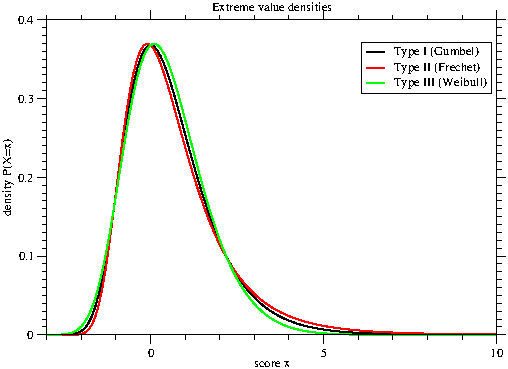
\includegraphics[width=2.8in]{figures/gev_density}
\end{minipage}
\begin{minipage}{3in}
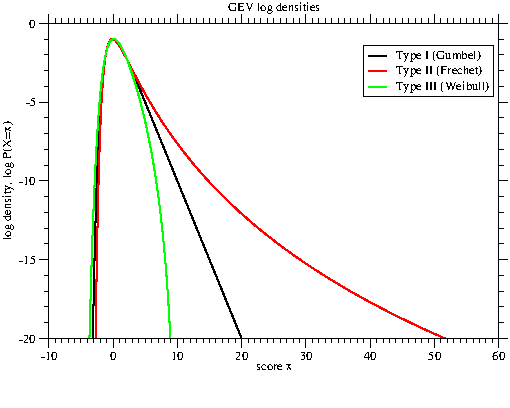
\includegraphics[width=2.8in]{figures/gev_logdensity}
\end{minipage}
}

For more details, see the excellent description in \citep{Coles01}.
Easel's $\{ \mu, \lambda, \alpha \}$ notation differs from the $\{
\mu, \sigma, \xi \}$ parameterization used by Coles. Use $\lambda =
\frac{1}{\sigma}$ and $\alpha = \xi$ to translate.

\subsection{Fitting GEV distributions to observed data}

Easel fits GEVs by maximum likelihood estimation by numerically
optimizing the log likelihood function, using first derivative
information and conjugate gradient descent.  See the \eslmod{gumbel}
chapter for a more general introduction to maximum likelihood fitting.

\subsubsection{Maximum likelihood estimation, complete data}

The function \ccode{esl\_gev\_FitComplete()} uses gradient information
to find parameters that optimize the likelihood function, using the
conjugate gradient descent code in the \eslmod{minimizer} module.

Given $n$ samples $x_1..x_n$, we want to estimate maximum likelihood
parameter estimates $\{ \hat{\mu}, \hat{\lambda}, \hat{\alpha} \}$
that maximize the log likelihood:

\begin{equation}
\log L(\lambda, \mu, \alpha) = n \log \lambda 
       - \frac{\alpha+1}{\alpha} 
           \sum_{i=1}^{n} \log\left[1+ \alpha\lambda(x_i - \mu) \right]
       - \sum_{i=1}^{n} \left[ 1 + \alpha\lambda (x_i - \mu) \right]^{\frac{1}{\alpha}}
\label{eqn:gev_logL}
\end{equation}

The $\left[ 1 + \alpha\lambda (x_i - \mu) \right]^{\frac{1}{\alpha}}$
term can be rewritten in a more conveniently differentiable form as
$\exp \left\{ \frac{1}{\alpha} \log \left[ 1 + \alpha\lambda (x_i - \mu)
\right] \right\}$.

Since the $\lambda$ parameter is constrained to $\lambda > 0$ but the
numerical optimizer expects unconstrained parameters, we use a change
of variables $\lambda = e^w$ and optimize an unconstrained value $w$.

The gradient of the log likelihood with respect to $\mu$, $w$, and
$\alpha$ is:

%% xref: STL9/118-120
\begin{eqnarray}
\frac{\partial \log L}{\partial \mu} & = &
  \sum_{i=1}^n \frac{\lambda (\alpha+1)}{1+\alpha\lambda(x_i-\mu)} 
 -\sum_{i=1}^n \lambda \exp 
    \left\{ -\frac{\alpha+1}{\alpha} \log
          \left[1+\alpha\lambda(x_i-\mu)\right] \right\}
\\%
\label{eqn:gev_mupartial}
\frac{\partial \log L}{\partial w} & = &
  n - \sum_{i=1}^{n} \frac{\lambda (\alpha+1) (x_i - \mu)} 
                          {1 + \alpha \lambda (x_i - \mu)}
  + \sum_{i=1}^n \lambda (x_i - \mu) 
         \exp \left\{ -\frac{\alpha+1}{\alpha} \log
          \left[1+\alpha\lambda(x_i-\mu)\right] \right\}
\\%
\label{eqn:gev_wpartial}
\frac{\partial \log L}{\partial \alpha} & = &
   \sum_{i=1}^n \left\{
      \begin{array}{l}
      - \frac{\alpha+1}{\alpha} \frac{\lambda(x_i-\mu)}
                                  {1 +\alpha\lambda(x_i-\mu)}\\
      + \frac{1}{\alpha^2} \log \left[ 1 + \alpha\lambda(x_i - \mu) \right]\\
      + \frac{1}{\alpha} \frac{\lambda(x_i-\mu)}
                          {1 +\alpha\lambda(x_i-\mu)}
      e^{-\frac{1}{\alpha} \log\left[ 1 + \alpha\lambda(x_i - \mu) \right]}\\
     -  \frac{1}{\alpha^2} \log \left[ 1 + \alpha\lambda(x_i - \mu) \right]
      e^{-\frac{1}{\alpha} \log\left[ 1 + \alpha\lambda(x_i - \mu)
	 \right]} 
     \end{array}
     \right.
\\%
\label{eqn:gev_alphapartial}
\end{eqnarray}

When $|\alpha\lambda(x_i - \mu)|$ approaches $0$, the GEV approximates
a Gumbel distribution and these equations can be simplified using the
approximation $\log(1+a) \simeq a$.








\subsection{Functions in the gev module}
\begin{sreapi}
\hypertarget{func:esl_gev_pdf()}
{\item[double esl\_gev\_pdf(double x, double mu, double lambda, double alpha)]}

Calculates the probability density function for the 
generalized extreme value distribution, $P(X=x)$, given
quantile \ccode{x} and GEV location, scale, shape parameters 
\ccode{mu}, \ccode{lambda}, \ccode{alpha}.


\hypertarget{func:esl_gev_logpdf()}
{\item[double esl\_gev\_logpdf(double x, double mu, double lambda, double alpha)]}

Calculates the log probability density function for the
generalized extreme value distribution, $\log P(X=x)$, 
given quantile \ccode{x} and GEV location, scale, shape
parameters \ccode{mu}, \ccode{lambda}, \ccode{alpha}.


\hypertarget{func:esl_gev_cdf()}
{\item[double esl\_gev\_cdf(double x, double mu, double lambda, double alpha)]}

Calculates the cumulative distribution function for the
generalized extreme value distribution, $P(X \leq x)$, 
given quantile \ccode{x} and GEV location, scale, shape
parameters \ccode{mu}, \ccode{lambda}, \ccode{alpha}.


\hypertarget{func:esl_gev_logcdf()}
{\item[double esl\_gev\_logcdf(double x, double mu, double lambda, double alpha)]}

Calculates the log of the cumulative distribution function for a
generalized extreme value distribution, $\log P(X \leq x)$, 
given quantile \ccode{x} and GEV location, scale, shape
parameters \ccode{mu}, \ccode{lambda}, \ccode{alpha}.


\hypertarget{func:esl_gev_surv()}
{\item[double esl\_gev\_surv(double x, double mu, double lambda, double alpha)]}

Calculates the survivor function, $P(X>x)$ (that is, 1-cdf),
the right tail's probability mass,  given quantile \ccode{x} and
GEV location, scale, shape parameters \ccode{mu}, \ccode{lambda}, \ccode{alpha}.


\hypertarget{func:esl_gev_logsurv()}
{\item[double esl\_gev\_logsurv(double x, double mu, double lambda, double alpha)]}

Calculates the log survivor function $\log P(X>x)$ for a 
generalized extreme value distribution (that is, 
$\log (1 - \mbox{cdf})$, the log of the right tail's probability
mass), given quantile \ccode{x} and GEV location, scale, shape
parameters \ccode{mu}, \ccode{lambda}, \ccode{alpha}.


\hypertarget{func:esl_gev_invcdf()}
{\item[double esl\_gev\_invcdf(double p, double mu, double lambda, double alpha)]}

Calculates the inverse CDF of the GEV: given a probability
\ccode{p} ($0 < p < 1$), returns the quantile \ccode{x} which would
give \ccode{p} as its CDF, for a generalized extreme value 
distribution with parameters \ccode{mu}, \ccode{lambda}, and \ccode{alpha}.


\hypertarget{func:esl_gev_generic_pdf()}
{\item[double esl\_gev\_generic\_pdf(double x, void *params)]}

Generic-API version of PDF.


\hypertarget{func:esl_gev_generic_cdf()}
{\item[double esl\_gev\_generic\_cdf(double x, void *params)]}

Generic-API version of CDF.


\hypertarget{func:esl_gev_generic_surv()}
{\item[double esl\_gev\_generic\_surv(double x, void *params)]}

Generic-API version of survival function.


\hypertarget{func:esl_gev_generic_invcdf()}
{\item[double esl\_gev\_generic\_invcdf(double p, void *params)]}

Generic-API version of inverse CDF.


\hypertarget{func:esl_gev_Plot()}
{\item[int esl\_gev\_Plot(FILE *fp, double mu, double lambda, double alpha,
	     double (*func)(double x, double mu, double lambda, double alpha), 
	     double xmin, double xmax, double xstep)]}

Plot some GEV function \ccode{func} (for instance,
\ccode{esl\_gev\_pdf()}) for parameters \ccode{mu} and \ccode{lambda}, for
a range of quantiles x from \ccode{xmin} to \ccode{xmax} in steps of \ccode{xstep};
output to an open stream \ccode{fp} in xmgrace XY input format.

Returns \ccode{eslOK} on success.

Throws \ccode{eslEWRITE} on any system write error, such as filled disk.


\hypertarget{func:esl_gev_Sample()}
{\item[double esl\_gev\_Sample(ESL\_RANDOMNESS *r, double mu, double lambda, double alpha)]}

Sample a GEV-distributed random variate,
by the transformation method.


\hypertarget{func:esl_gev_FitComplete()}
{\item[int esl\_gev\_FitComplete(double *x, int n, 
		    double *ret\_mu, double *ret\_lambda, double *ret\_alpha)]}

Given an array of \ccode{n} GEV-distributed samples \ccode{x[0]..x[n-1},
return maximum likelihood parameters \ccode{ret\_mu}, 
\ccode{ret\_lambda}, and \ccode{ret\_alpha}.

Uses a conjugate gradient descent algorithm that
can be computationally intensive. A typical problem
involving 10,000-100,000 points may take a second 
to solve.

Returns \ccode{eslOK} on success.

Throws \ccode{eslENOHALT} if the fit doesn't converge.



\hypertarget{func:esl_gev_FitCensored()}
{\item[int esl\_gev\_FitCensored(double *x, int n, int z, double phi,
		    double *ret\_mu, double *ret\_lambda, double *ret\_alpha)]}

Given a left-censored array of \ccode{n} GEV-distributed samples
\ccode{x[0]..x[n-1}, the number of censored samples \ccode{z}, and
the censoring value \ccode{phi} (where all $x_i > \phi$ and
all $z$ censored samples are $\leq \phi$);
return maximum likelihood parameters \ccode{ret\_mu}, 
\ccode{ret\_lambda}, and \ccode{ret\_alpha}.

Returns \ccode{eslOK} on success.

Throws \ccode{eslENOHALT} if the fit doesn't converge.



\end{sreapi}


}{}

\ifthenelse{\boolean{completedraft}}{
\newpage
\section{\eslmodincmd{gumbel}: Type I extreme value (Gumbel) statistics}
./../esl_gumbel.tex
\subsection{Functions in the gumbel module}
\begin{sreapi}
\hypertarget{func:esl_gumbel_pdf()}
{\item[double esl\_gumbel\_pdf(double x, double mu, double lambda)]}

Calculates the probability density function for the Gumbel,
$P(X=x)$, given quantile \ccode{x} and Gumbel location and
scale parameters \ccode{mu} and \ccode{lambda}.

Let $y = \lambda(x-\mu)$; for 64-bit doubles,
useful dynamic range is about $-6.5 <= y <= 710$.
Returns 0.0 for smaller $y$, 0.0 for larger $y$.


\hypertarget{func:esl_gumbel_logpdf()}
{\item[double esl\_gumbel\_logpdf(double x, double mu, double lambda)]}

Calculates the log probability density function for the Gumbel,
$\log P(X=x)$.

Let $y = \lambda(x-\mu)$; for 64-bit doubles,
useful dynamic range is about $-708 <= y <= \infty$.
Returns $-\infty$ for smaller or larger $y$.


\hypertarget{func:esl_gumbel_cdf()}
{\item[double esl\_gumbel\_cdf(double x, double mu, double lambda)]}

Calculates the cumulative distribution function
for the Gumbel, $P(X \leq x)$.

Let $y = \lambda(x-\mu)$; for 64-bit doubles,
useful dynamic range for $y$ is about $-6.5 <= y <=36$.
Returns 0.0 for smaller $y$, 1.0 for larger $y$.


\hypertarget{func:esl_gumbel_logcdf()}
{\item[double esl\_gumbel\_logcdf(double x, double mu, double lambda)]}

Calculates the log of the cumulative distribution function
for the Gumbel, $\log P(X \leq x)$.

Let $y = \lambda(x-\mu)$; for 64-bit doubles,
useful dynamic range for $y$ is about $-708 <= y <= 708$.
Returns $-\infty$ for smaller $y$, 0.0 for larger $y$.


\hypertarget{func:esl_gumbel_surv()}
{\item[double esl\_gumbel\_surv(double x, double mu, double lambda)]}

Calculates the survivor function, $P(X>x)$ for a Gumbel 
(that is, 1-cdf), the right tail's probability mass.

Let $y=\lambda(x-\mu)$; for 64-bit doubles, 
useful dynamic range for $y$ is $-3.6 <= y <= 708$.
Returns 1.0 for $y$ below lower limit, and 0.0
for $y$ above upper limit.


\hypertarget{func:esl_gumbel_logsurv()}
{\item[double esl\_gumbel\_logsurv(double x, double mu, double lambda)]}

Calculates $\log P(X>x)$ for a Gumbel (that is, $\log$(1-cdf)):
the log of the right tail's probability mass.

Let $y=\lambda(x-\mu)$; for 64-bit doubles, 
useful dynamic range for $y$ is $-6.5 <= y <= \infty$.
Returns 0.0 for smaller $y$.


\hypertarget{func:esl_gumbel_invcdf()}
{\item[double esl\_gumbel\_invcdf(double p, double mu, double lambda)]}

Calculates the inverse CDF for a Gumbel distribution
with parameters \ccode{mu} and \ccode{lambda}. That is, returns
the quantile \ccode{x} at which the CDF is \ccode{p}.


\hypertarget{func:esl_gumbel_invsurv()}
{\item[double esl\_gumbel\_invsurv(double p, double mu, double lambda)]}

Calculates the score at which the right tail's mass
is p, for a Gumbel distribution
with parameters \ccode{mu} and \ccode{lambda}. That is, returns
the quantile \ccode{x} at which 1-CDF is \ccode{p}.


\hypertarget{func:esl_gumbel_generic_pdf()}
{\item[double esl\_gumbel\_generic\_pdf(double p, void *params)]}

Generic-API version of PDF function.


\hypertarget{func:esl_gumbel_generic_cdf()}
{\item[double esl\_gumbel\_generic\_cdf(double x, void *params)]}

Generic-API version of CDF function.


\hypertarget{func:esl_gumbel_generic_surv()}
{\item[double esl\_gumbel\_generic\_surv(double p, void *params)]}

Generic-API version of survival function.


\hypertarget{func:esl_gumbel_generic_invcdf()}
{\item[double esl\_gumbel\_generic\_invcdf(double p, void *params)]}

Generic-API version of inverse CDF.


\hypertarget{func:esl_gumbel_Plot()}
{\item[int esl\_gumbel\_Plot(FILE *fp, double mu, double lambda, 
		double (*func)(double x, double mu, double lambda), 
		double xmin, double xmax, double xstep)]}

Plot a Gumbel function \ccode{func} (for instance,
\ccode{esl\_gumbel\_pdf()}) for parameters \ccode{mu} and \ccode{lambda}, for
a range of quantiles x from \ccode{xmin} to \ccode{xmax} in steps of \ccode{xstep};
output to an open stream \ccode{fp} in xmgrace XY input format.

Returns \ccode{eslOK} on success.

Throws \ccode{eslEWRITE} on any system write error, such as filled disk.


\hypertarget{func:esl_gumbel_Sample()}
{\item[double esl\_gumbel\_Sample(ESL\_RANDOMNESS *r, double mu, double lambda)]}

Sample a Gumbel-distributed random variate
by the transformation method.


\hypertarget{func:esl_gumbel_FitComplete()}
{\item[int esl\_gumbel\_FitComplete(double *x, int n, double *ret\_mu, double *ret\_lambda)]}

Given an array of Gumbel-distributed samples
\ccode{x[0]..x[n-1]}, find maximum likelihood parameters \ccode{mu}
and \ccode{lambda}.

The number of samples \ccode{n} must be reasonably large to get
an accurate fit. \ccode{n=100} suffices to get an accurate
location parameter $\mu$ (to about 1% error), but
\ccode{n~10000} is required to get a similarly accurate
estimate of $\lambda$. It's probably a bad idea to try to
fit a Gumbel to less than about 1000 data points.

On a very small number of samples, the fit can fail
altogether, in which case the routine will return a
\ccode{eslENORESULT} code. Caller must check for this.

Uses approach described in [Lawless82]. Solves for lambda
using Newton/Raphson iterations, then substitutes lambda
into Lawless' equation 4.1.5 to get mu.

Returns \ccode{eslOK} on success.

\ccode{eslEINVAL} if n\ccode{=1.
<eslENORESULT} if the fit fails, likely because the
number of samples is too small. On either error,
\ccode{*ret\_mu} and \ccode{*ret\_lambda} are 0.0.  These are classed
as failures (normal errors) because the data vector may
have been provided by a user.


\hypertarget{func:esl_gumbel_FitCompleteLoc()}
{\item[int esl\_gumbel\_FitCompleteLoc(double *x, int n, double lambda, double *ret\_mu)]}

Given an array of Gumbel-distributed samples 
\ccode{x[0]..x[n-1]} (complete data), and a known
(or otherwise fixed) \ccode{lambda}, find a maximum
likelihood estimate for location parameter \ccode{mu}.

Algorithm is a straightforward simplification of
\ccode{esl\_gumbel\_FitComplete()}.

Returns \ccode{eslOK} on success.

\ccode{eslEINVAL} if n\ccode{=1; on this error, <*ret\_mu} = 0.

Throws (no abnormal error conditions)


\hypertarget{func:esl_gumbel_FitCensored()}
{\item[int esl\_gumbel\_FitCensored(double *x, int n, int z, double phi, double *ret\_mu, double *ret\_lambda)]}

Given a left-censored array of Gumbel-distributed samples
\ccode{x[0]..x[n-1]}, the number of censored samples \ccode{z}, and
the censoring value \ccode{phi} (all \ccode{x[i]} $\geq$ \ccode{phi}).  Find
maximum likelihood parameters \ccode{mu} and \ccode{lambda}.

Returns \ccode{eslOK} on success.

\ccode{eslEINVAL} if n\ccode{=1. 
<eslENORESULT} if the fit fails, likey because the number
of samples is too small.
On either error, \ccode{*ret\_mu} and \ccode{*ret\_lambda} are 0.0.
These are classed as failures (normal errors) because the
data vector may have been provided by a user.


\hypertarget{func:esl_gumbel_FitCensoredLoc()}
{\item[int esl\_gumbel\_FitCensoredLoc(double *x, int n, int z, double phi, double lambda, 
			  double *ret\_mu)]}

Given a left-censored array of Gumbel distributed samples
\ccode{x[0}..x[n-1]>, the number of censored samples \ccode{z}, and the censoring
value \ccode{phi} (where all \ccode{x[i]} $\geq$ \ccode{phi}), and a known
(or at least fixed) \ccode{lambda};
find the maximum likelihood estimate of the location
parameter $\mu$ and return it in \ccode{ret\_mu}.

Returns \ccode{eslOK} on success.

\ccode{eslEINVAL} if n\ccode{=1; on this error, <*ret\_mu} = 0.

Throws (no abnormal error conditions)


\hypertarget{func:esl_gumbel_FitTruncated()}
{\item[int esl\_gumbel\_FitTruncated(double *x, int n, double phi, double *ret\_mu, double *ret\_lambda)]}

Given a left-truncated array of Gumbel-distributed
samples \ccode{x[0]..x[n-1]} and the truncation threshold
\ccode{phi} (such that all \ccode{x[i]} $\geq$ \ccode{phi}).
Find maximum likelihood parameters \ccode{mu} and \ccode{lambda}.

\ccode{phi} should not be much greater than \ccode{mu}, the
mode of the Gumbel, or the fit will become unstable
or may even fail to converge. The problem is
that for \ccode{phi} $>$ \ccode{mu}, the tail of the Gumbel
becomes a scale-free exponential, and \ccode{mu} becomes
undetermined.

Returns \ccode{eslOK} on success.

\ccode{eslEINVAL} if n\ccode{=1.
<eslENORESULT} if the fit fails, likely because the
number of samples \ccode{n} is too small, or because the
truncation threshold is high enough that the tail
looks like a scale-free exponential and we can't
obtain \ccode{mu}.
On either error, \ccode{*ret\_mu} and \ccode{*ret\_lambda} are 
returned as 0.0.
These are "normal" (returned) errors because 
the data might be provided directly by a user.

Throws \ccode{eslEMEM} on allocation error.           


\end{sreapi}


}{}

\ifthenelse{\boolean{completedraft}}{
\newpage
\section{\eslmodincmd{hyperexp}: Hyperexponential distributions}
./../esl_hyperexp.tex
\subsection{Functions in the hyperexp module}
\begin{sreapi}
\hypertarget{func:esl_hyperexp_Create()}
{\item[ESL\_HYPEREXP * esl\_hyperexp\_Create(int K)]}

Creates an object to hold parameters for a \ccode{K}-component
hyperexponential. 

Parameters in the object are initialized 
($q_k = \frac{1}{K}$, $\lambda_k = 1$, $\mu = 0$), but
the caller will want to set these according to its own
purposes.

Returns ptr to newly allocated/initialized \ccode{ESL\_HYPEREXP} object.

Throws NULL on allocation failure.


\hypertarget{func:esl_hyperexp_Destroy()}
{\item[void esl\_hyperexp\_Destroy(ESL\_HYPEREXP *h)]}

Deallocates the hyperexponential parameter object \ccode{h}.

Returns (void).


\hypertarget{func:esl_hyperexp_Copy()}
{\item[int esl\_hyperexp\_Copy(ESL\_HYPEREXP *src, ESL\_HYPEREXP *dest)]}

Makes a copy of the hyperexponential parameter object \ccode{src}
in \ccode{dest}. Caller must have already allocated \ccode{dest} to have
(at least) the same number of components as \ccode{src}.

Returns \ccode{eslOK} on success.

Throws \ccode{eslEINCOMPAT} if \ccode{dest} isn't allocated with enough
components to hold a copy of \ccode{src}.


\hypertarget{func:esl_hyperexp_FixedUniformMixture()}
{\item[int esl\_hyperexp\_FixedUniformMixture(ESL\_HYPEREXP *h)]}

Set the mixture coeffients to a uniform (1/K) distribution,
and fix them there so they aren't estimable parameters.


\hypertarget{func:esl_hyperexp_SortComponents()}
{\item[int esl\_hyperexp\_SortComponents(ESL\_HYPEREXP *h)]}

Rearrange the components in a hyperexponential in
order of lambda values, with the highest lambda first.

Stupid $O(K^2)$ selection sort algorithm here, because we
expect $K$ to be small.


\hypertarget{func:esl_hyperexp_Write()}
{\item[int esl\_hyperexp\_Write(FILE *fp, ESL\_HYPEREXP *hxp)]}

Write hyperexponential parameters from \ccode{hxp} to an open \ccode{fp}.

The output format is suitable for input by \ccode{esl\_hyperexp\_Read()}.

Returns \ccode{eslOK} on success.

Throws \ccode{eslEWRITE} on any write error.


\hypertarget{func:esl_hyperexp_Dump()}
{\item[int esl\_hyperexp\_Dump(FILE *fp, ESL\_HYPEREXP *hxp)]}

Dump hyperexponential parameters from \ccode{hxp} to an open \ccode{fp},
all on one line with no comments.

The output format is suitable for input by
\ccode{esl\_hyperexp\_Read()}, like \ccode{esl\_hyperexp\_Write()},
though it's intended as a diagnostic dump of the
contents of the object.

Returns \ccode{eslOK} on success.


\hypertarget{func:esl_hxp_pdf()}
{\item[double esl\_hxp\_pdf(double x, ESL\_HYPEREXP *h)]}

Returns the probability density function $P(X=x)$ for
quantile \ccode{x}, given hyperexponential parameters \ccode{h}.


\hypertarget{func:esl_hxp_logpdf()}
{\item[double esl\_hxp\_logpdf(double x, ESL\_HYPEREXP *h)]}

Returns the log of the PDF ($\log P(X=x)$) for quantile \ccode{x},
given hyperexponential parameters \ccode{h}.


\hypertarget{func:esl_hxp_cdf()}
{\item[double esl\_hxp\_cdf(double x, ESL\_HYPEREXP *h)]}

Returns the cumulative distribution function $P(X \leq x)$
for quantile \ccode{x}, given hyperexponential parameters \ccode{h}.


\hypertarget{func:esl_hxp_logcdf()}
{\item[double esl\_hxp\_logcdf(double x, ESL\_HYPEREXP *h)]}

Returns the log of the CDF $\log P(X \leq x)$
for quantile \ccode{x}, given hyperexponential parameters \ccode{h}.


\hypertarget{func:esl_hxp_surv()}
{\item[double esl\_hxp\_surv(double x, ESL\_HYPEREXP *h)]}

Returns the survivor function $P(X > x)$ (1-CDF)
for quantile \ccode{x}, given hyperexponential parameters \ccode{h}.


\hypertarget{func:esl_hxp_logsurv()}
{\item[double esl\_hxp\_logsurv(double x, ESL\_HYPEREXP *h)]}

Returns the log survivor function $\log P(X > x)$ (log(1-CDF))
for quantile \ccode{x}, given hyperexponential parameters \ccode{h}.


\hypertarget{func:esl_hxp_invcdf()}
{\item[double esl\_hxp\_invcdf(double p, ESL\_HYPEREXP *h)]}

Calculates the inverse CDF for a hyperexponential \ccode{h}
returning the quantile \ccode{x} at which the CDF is \ccode{p}.

The inverse CDF of a mixture model has no
analytical expression as far as I'm aware. The calculation
here is a computationally expensive, brute force bisection
search in \ccode{x} using the CDF function. It will suffice for
a small number of calls (for plotting applications, for example),
but it is not sufficient for a large number of calls.


\hypertarget{func:esl_hxp_generic_pdf()}
{\item[double esl\_hxp\_generic\_pdf(double x, void *params)]}

Generic-API version of PDF call.


\hypertarget{func:esl_hxp_generic_cdf()}
{\item[double esl\_hxp\_generic\_cdf(double x, void *params)]}

Generic-API version of CDF call.


\hypertarget{func:esl_hxp_generic_surv()}
{\item[double esl\_hxp\_generic\_surv(double x, void *params)]}

Generic-API version of survivor function.


\hypertarget{func:esl_hxp_generic_invcdf()}
{\item[double esl\_hxp\_generic\_invcdf(double p, void *params)]}

Generic-API version of inverse CDF.


\hypertarget{func:esl_hxp_Plot()}
{\item[int esl\_hxp\_Plot(FILE *fp, ESL\_HYPEREXP *h,
	     double (*func)(double x, ESL\_HYPEREXP *h), 
	     double xmin, double xmax, double xstep)]}

Plot some function \ccode{func} (for instance, \ccode{esl\_hxp\_pdf()})
for hyperexponential parameters \ccode{h}, for a range of
quantiles x from \ccode{xmin} to \ccode{xmax} in steps of \ccode{xstep};
output to an open stream \ccode{fp} in xmgrace XY input format.

Returns \ccode{eslOK} on success.

Throws \ccode{eslEWRITE} on any system write error. 


\hypertarget{func:esl_hxp_Sample()}
{\item[double esl\_hxp\_Sample(ESL\_RANDOMNESS *r, ESL\_HYPEREXP *h)]}

Sample a random variate x from a hyperexponential \ccode{h}, 
given random number source \ccode{r}.


\hypertarget{func:esl_hyperexp_Read()}
{\item[int esl\_hyperexp\_Read(ESL\_FILEPARSER *e, ESL\_HYPEREXP **ret\_hxp)]}

Reads hyperexponential parameters from an open \ccode{e}.
which is an \ccode{ESL\_FILEPARSER} tokenizer for an open stream.

The first token is \ccode{K}, the number of mixture components.
The second token is \ccode{mu}, the x offset shared by all components.
Then for each mixture component \ccode{k=1..K}, it reads
a mixture coefficient \ccode{q[k]} and a decay parameter
\ccode{lambda[k]}.

The \ccode{2K+2} data tokens must occur in this order, but
they can be grouped into any number of lines, because the
parser ignores line breaks.

Anything after a \ccode{\#} character on a line is a comment, and
is ignored.

Returns \ccode{eslOK} on success, and \ccode{ret\_hxp} points to a new \ccode{ESL\_HYPEREXP}
object.
\ccode{eslEFORMAT} on "normal" parse failure caused by a bad file 
format that's likely the user's fault.

Throws \ccode{eslEMEM} if allocation of the new \ccode{ESL\_HYPEREXP} fails.




\hypertarget{func:esl_hyperexp_ReadFile()}
{\item[int esl\_hyperexp\_ReadFile(char *filename, ESL\_HYPEREXP **ret\_hxp)]}

Convenience wrapper around \ccode{esl\_hyperexp\_Read()} that takes
a filename as an argument, instead of an open \ccode{ESL\_FILEPARSER}.

This lets you quickly read an object from a file, but it
limits your ability to deal gracefully and flexibly with
'normal' errors like 'file not found' or 'bad file format'.
Here, all errors are fatal.

Returns \ccode{eslOK} on success.

Throws \ccode{eslEMEM} on an allocation failure.

\ccode{eslEFORMAT} on any parse error. Diagnostic information is
unavailable, because the \ccode{ESL\_FILEPARSER} that's holding 
that information is internal to this function. 

\ccode{eslENOTFOUND} on any failure to open the file.


\hypertarget{func:esl_hxp_FitGuess()}
{\item[int esl\_hxp\_FitGuess(double *x, int n, ESL\_HYPEREXP *h)]}

Given a sorted vector of \ccode{n} observed data samples \ccode{x[]},
from smallest \ccode{x[0]} to largest \ccode{x[n-1]}, calculate a
very crude guesstimate of a fit -- suitable only as a starting
point for further optimization -- and return those parameters
in \ccode{h}.

Assigns $q_k \propto \frac{1}{k}$ and  $\mu = \min_i x_i$;
splits $x$ into $K$ roughly equal-sized bins, and
and assigns $\lambda_k$ as the ML estimate from bin $k$.
(If $q_k$ coefficients have already been fixed to 
known values, this step is skipped.)


\hypertarget{func:esl_hxp_FitComplete()}
{\item[int esl\_hxp\_FitComplete(double *x, int n, ESL\_HYPEREXP *h)]}

Given a vector of \ccode{n} observed data samples \ccode{x[]} 
(sorted or unsorted), and an initial guess \ccode{h} for
a hyperexponential, find maximum likelihood parameters
by conjugate gradient descent optimization, starting
from \ccode{h} and leaving the final optimized solution in
\ccode{h}.

Returns \ccode{eslOK} on success, and \ccode{h} contains the fitted 
hyperexponential parameters.

Throws \ccode{eslEMEM} on allocation error, and \ccode{h} is left in
in its initial state.           


\hypertarget{func:esl_hxp_FitGuessBinned()}
{\item[int esl\_hxp\_FitGuessBinned(ESL\_HISTOGRAM *g, ESL\_HYPEREXP *h)]}

Given a histogram \ccode{g} with binned observations;
obtain a very crude guesstimate of a fit -- suitable only 
as a starting point for further optimization -- and return 
those parameters in \ccode{h}.

Assigns $q_k \propto \frac{1}{k}$ and  $\mu = \min_i x_i$;
splits $x$ into $K$ roughly equal-sized bins, and
and assigns $\lambda_k$ as the ML estimate from bin $k$.
If the coefficients have already been set to known values,
this step is skipped.


\hypertarget{func:esl_hxp_FitCompleteBinned()}
{\item[int esl\_hxp\_FitCompleteBinned(ESL\_HISTOGRAM *g, ESL\_HYPEREXP *h)]}

Given a histogram \ccode{g} with binned observations, where each
bin i holds some number of observed samples x with values from 
lower bound l to upper bound u (that is, $l < x \leq u$),
and given a starting guess \ccode{h} for hyperexponential parameters;

Find maximum likelihood parameters \ccode{h} by conjugate gradient
descent, starting from the initial \ccode{h} and leaving the
optimized solution in \ccode{h}.

Returns \ccode{eslOK} on success.

Throws \ccode{eslEMEM} on allocation error, and \ccode{h} is left in its
initial state.


\end{sreapi}


}{}

\ifthenelse{\boolean{completedraft}}{
\newpage
\section{\eslmodincmd{mixdchlet}: Mixture Dirichlet distributions}
%\documentclass[11pt]{article}
\setcounter{secnumdepth}{0}

\usepackage{relsize}

\newcommand{\mono}[1]{{\smaller\texttt{#1}}}                    % literal (to be typed): code, program names

\begin{document}

\section{Fitting a mixture Dirichlet to counts}

\mono{esl\_mixdchlet\_Fit()} infers a maximum likelihood mixture
Dirichlet distribution for a data set of count vectors. It uses
conjugate gradient descent from an initial starting point. The result
is only a local optimum, so we typically run it multiple times with
different starting points. The partial derivatives of the log
likelihood function are persnickety, and the purpose of these notes is
to enshrine the derivation that corresponds to the implementation.

We have $N$ count vectors $c_i$, with each vector consisting of $K$
counts for individual symbols $c_{ia} \geq 0$. The mixture Dirichlet
$\theta$ consists of $Q$ components $\alpha_k$, with each parameter
vector containing $K$ parameters $\alpha_{ka} > 0$, and $Q$ mixture
coefficients $q_k > 0, \sum_k q_k = 1$.

The log likelihood of the data is:

\[
  L = \log P(\mbox{data} \mid \theta) = \sum_i \log P(c_i \mid \theta) = \sum_i \log \sum_k q_k P(c_i \mid \alpha_k)
\]

\mono{esl\_mixdchlet\_logpdf\_c()} calculates $\log P(c_i \mid
\theta)$.

$P(c_i \mid \alpha_k)$, the probability of one count vector given one
Dirichlet component, is:

\[
P(c_i \mid \alpha_k) = \frac{ |c_i|! }
                            { \prod_a c_{ia}! }
                       \frac{ \prod_a \Gamma \left( c_{ia} + \alpha_{ia} \right) }
                            { \Gamma ( |c_i + \alpha_k| ) }
                       \frac{ \Gamma ( |\alpha_k| ) }
                            { \prod_a \Gamma \left( \alpha_{ka} \right) }
\]

\mono{esl\_dirichlet\_logpdf\_c()} calculates $\log P(c_i \mid \alpha_k)$.

The conjugate gradient descent code works with unconstrained
real-valued parameters. The Dirichlet parameters $\alpha_{ka}$ are
constrained to $>0$, and mixture coefficients $q_k$ are constrained to
$>0$ and $\sum_k q_k = 1$. Define a change of variables in terms of
unconstrained parameters $\lambda_k$ for the mixture coefficients and
$\beta_{ka}$ for Dirichlet parameters:

\begin{eqnarray*}
  q_k          & = & \frac{ e^{\lambda_k} } { \sum_m e^{\lambda_m} } \\
  \alpha_{ka}  & = & e^{\beta_{ka}} 
\end{eqnarray*}

After variable substitution, partial differentiation w.r.t. the
unconstrained parameters, and substituting back the original
parameters, we have for the mixture coefficients:

\[
  \frac{\partial L}{\partial \lambda_k} = \sum_i P(k \mid \theta, c_i) - q_k
\]

i.e., the difference between the posterior probability of component
$k$ $P(k \mid \theta, c_i)$, calculated by \mono{mixdchlet\_postq()},
and its prior $q_k$.

For the Dirichlet parameters:

\[
\frac{\partial L}{\partial \beta_{ka}}  =  \sum_i
 \alpha_{ka} P(k \mid \theta, c_i) 
    \left( \Psi \left( c_{ia} + \alpha_{ka} \right)  
        -  \Psi \left( | c_i | + | \alpha_k | \right)
        +  \Psi \left( | \alpha_k | \right) 
        -  \Psi \left( \alpha_{ka} \right) 
    \right) 
\]


$\Psi(x)$ is the digamma function $\frac{d}{dx} \log \Gamma(x) =
\frac{\Gamma'(x)}{\Gamma(x)}$, for $x > 0$, implemented by
\mono{esl\_stats\_Psi()}.

The Easel conjugate gradient descent optimizer is a minimizer, not a
maximizer.  The implementation provides the negative log likelihood
and the negative gradient to the CG routine.


\end{document}


\subsection{Functions in the mixdchlet module}
%\input{autotext/esl_mixdchlet_functions}
}{}

\ifthenelse{\boolean{completedraft}}{
\newpage
\section{\eslmodincmd{mixgev}: Mixture generalized extreme value distributions}
%\input{esl_mixgev}
%\subsection{Functions in the mixgev module}
%\input{autotext/esl_mixgev_functions}
}{}

\ifthenelse{\boolean{completedraft}}{
\newpage
\section{\eslmodincmd{normal}: Normal (Gaussian) distributions}
./../esl_normal.tex
\subsection{Functions in the normal module}
\begin{sreapi}
\hypertarget{func:esl_normal_pdf()}
{\item[double esl\_normal\_pdf(double x, double mu, double sigma)]}

Calculates the normal (Gaussian) probability density
function $P(X=x)$ for a normal distribution, given
value \ccode{x}, mean \ccode{mu}, and standard deviation \ccode{sigma}.



\hypertarget{func:esl_normal_logpdf()}
{\item[double esl\_normal\_logpdf(double x, double mu, double sigma)]}

Calculates the log of the probabiility density function
for the normal (Gaussian), $\log P(X=x)$, given value
\ccode{x}, mean \ccode{mu}, and standard deviation \ccode{sigma}.



\hypertarget{func:esl_normal_cdf()}
{\item[double esl\_normal\_cdf(double x, double mu, double sigma)]}

Calculates the cumulative distribution function for the
normal, $P(X \leq x)$, given value \ccode{x}, mean \ccode{mu},
and standard deviation \ccode{sigma}.



\hypertarget{func:esl_normal_surv()}
{\item[double esl\_normal\_surv(double x, double mu, double sigma)]}

Calculates the survivor function, $P(X>x)$ (that is,
1-CDF, the right tail probability mass) for a normal
distribution, given value \ccode{x}, mean \ccode{mu}, and standard
deviation \ccode{sigma}.



\end{sreapi}


}{}

\ifthenelse{\boolean{completedraft}}{
\newpage
\section{\eslmodincmd{stretchexp}: Stretched exponential distributions}
./../esl_stretchexp.tex
\subsection{Functions in the stretchexp module}
\begin{sreapi}
\hypertarget{func:esl_sxp_pdf()}
{\item[double esl\_sxp\_pdf(double x, double mu, double lambda, double tau)]}

Calculates the probability density function for the 
stretched exponential pdf, $P(X=x)$, given
quantile \ccode{x}, offset \ccode{mu}, and parameters \ccode{lambda} and \ccode{tau}.


\hypertarget{func:esl_sxp_logpdf()}
{\item[double esl\_sxp\_logpdf(double x, double mu, double lambda, double tau)]}

Calculates the log probability density function for the 
stretched exponential pdf, $\log P(X=x)$, given
quantile \ccode{x}, offset \ccode{mu}, and parameters \ccode{lambda} and \ccode{tau}.


\hypertarget{func:esl_sxp_cdf()}
{\item[double esl\_sxp\_cdf(double x, double mu, double lambda, double tau)]}

Calculates the cumulative distribution function for the 
stretched exponential pdf, $P(X \leq x)$, given
quantile \ccode{x}, offset \ccode{mu}, and parameters \ccode{lambda} and \ccode{tau}.


\hypertarget{func:esl_sxp_logcdf()}
{\item[double esl\_sxp\_logcdf(double x, double mu, double lambda, double tau)]}

Calculates the log of the cumulative distribution function for the 
stretched exponential pdf, $\log P(X \leq x)$, given
quantile \ccode{x}, offset \ccode{mu}, and parameters \ccode{lambda} and \ccode{tau}.


\hypertarget{func:esl_sxp_surv()}
{\item[double esl\_sxp\_surv(double x, double mu, double lambda, double tau)]}

Calculates the survival function for the 
stretched exponential pdf, $P(X > x)$, given
quantile \ccode{x}, offset \ccode{mu}, and parameters \ccode{lambda} and \ccode{tau}.


\hypertarget{func:esl_sxp_logsurv()}
{\item[double esl\_sxp\_logsurv(double x, double mu, double lambda, double tau)]}

Calculates the log survival function for the 
stretched exponential pdf, $\log P(X > x)$, given
quantile \ccode{x}, offset \ccode{mu}, and parameters \ccode{lambda} and \ccode{tau}.


\hypertarget{func:esl_sxp_invcdf()}
{\item[double esl\_sxp\_invcdf(double p, double mu, double lambda, double tau)]}

Calculates the inverse CDF for a stretched exponential
with parameters \ccode{mu}, \ccode{lambda}, and \ccode{tau}, returning
the quantile \ccode{x} at which the CDF is \ccode{p}.

The inverse CDF of the stretched exponential has no
analytical expression as far as I'm aware. The calculation
here is a computationally expensive, brute force bisection
search in \ccode{x} using the CDF function. It will suffice for
a small number of calls (for plotting applications, for example),
but it is not sufficient for a large number of calls.


\hypertarget{func:esl_sxp_generic_pdf()}
{\item[double esl\_sxp\_generic\_pdf(double x, void *params)]}

Generic-API wrapper around \ccode{esl\_sxp\_pdf()}, taking
a void ptr to a double array containing $\mu$, $\lambda$,
$\tau$ parameters.


\hypertarget{func:esl_sxp_generic_cdf()}
{\item[double esl\_sxp\_generic\_cdf(double x, void *params)]}

Generic-API wrapper around \ccode{esl\_sxp\_cdf()}, taking
a void ptr to a double array containing $\mu$, $\lambda$,
$\tau$ parameters.


\hypertarget{func:esl_sxp_generic_surv()}
{\item[double esl\_sxp\_generic\_surv(double x, void *params)]}

Generic-API wrapper around \ccode{esl\_sxp\_surv()}, taking
a void ptr to a double array containing $\mu$, $\lambda$,
$\tau$ parameters.


\hypertarget{func:esl_sxp_generic_invcdf()}
{\item[double esl\_sxp\_generic\_invcdf(double p, void *params)]}

Generic-API wrapper around \ccode{esl\_sxp\_invcdf()}, taking
a void ptr to a double array containing $\mu$, $\lambda$,
$\tau$ parameters.


\hypertarget{func:esl_sxp_Plot()}
{\item[int esl\_sxp\_Plot(FILE *fp, double mu, double lambda, double tau,
	     double (*func)(double x, double mu, double lambda, double tau), 
	     double xmin, double xmax, double xstep)]}

Plot some stretched exponential function \ccode{func} (for instance,
\ccode{esl\_sxp\_pdf()}) for parameters \ccode{mu}, \ccode{lambda}, and \ccode{tau}, for
a range of quantiles x from \ccode{xmin} to \ccode{xmax} in steps of \ccode{xstep};
output to an open stream \ccode{fp} in xmgrace XY input format.

Returns \ccode{eslOK} on success.

Throws \ccode{eslEWRITE} on any system write error, such as filled disk.


\hypertarget{func:esl_sxp_Sample()}
{\item[double esl\_sxp\_Sample(ESL\_RANDOMNESS *r, double mu, double lambda, double tau)]}

Sample a stretched exponential random variate,
by a change of variable from a Gamma sample.


\hypertarget{func:esl_sxp_FitComplete()}
{\item[int esl\_sxp\_FitComplete(double *x, int n,
		    double *ret\_mu, double *ret\_lambda, double *ret\_tau)]}

Given a vector of \ccode{n} observed data samples \ccode{x[]},
find maximum likelihood parameters by conjugate gradient 
descent optimization.


\hypertarget{func:esl_sxp_FitCompleteBinned()}
{\item[int esl\_sxp\_FitCompleteBinned(ESL\_HISTOGRAM *g,
			  double *ret\_mu, double *ret\_lambda, double *ret\_tau)]}

Given a histogram \ccode{g} with binned observations, where each
bin i holds some number of observed samples x with values from 
lower bound l to upper bound u (that is, $l < x \leq u$);
find maximum likelihood parameters mu, lambda, tau by conjugate
gradient descent optimization.


\end{sreapi}


}{}

\ifthenelse{\boolean{completedraft}}{
\newpage
\section{\eslmodincmd{weibull}: Weibull distributions}

The Weibull distribution may be useful for fitting fat-tailed
empirical distributions.

In the literature, the Weibull is sometimes called a ``stretched
exponential'' distribution when its shape parameter $\tau$ is less
than 1. ``Stretched exponential'' distributions in the literature are
either Weibull (PDF $ = \lambda \tau (\lambda x)^\tau exp\left[-
(\lambda x)^tau \right]$ or a more simple PDF $\propto exp\left[-
{\lambda(x-\mu)}^tau \right]$. Easel treats the latter form in the
\eslmod{stretchexp} module.

\subsection{Weibull densities}

The probability density function (PDF) is:

\begin{equation}
P(X=x) = \lambda \tau [\lambda(x - \mu)]^{\tau-1} e^{- [\lambda(x-\mu)]^{\tau}}
\label{eqn:weibull_pdf}
\end{equation}

The cumulative distribution function (CDF) is:

\begin{equation}
P(X \leq x) = 1 - e^{- [\lambda(x-\mu)]^{\tau}}
\label{eqn:weibull_cdf}
\end{equation}

Variate $x$ ranges $\mu \leq x < \infty$. (However, for $\tau < 1$,
the PDF goes to infinity at $x=\mu$, so evaluating at $x=\mu$ may not
be desired.)

Location parameter $\mu$ is unconstrained, $-\infty < \mu <
\infty$. (Weibull distributions are usually represented without an
explicit location parameter, implicitly assuming $\mu = 0$.)

Scale parameter $\lambda$ is nonnegative, $\lambda >
0$. (Alteratively, Weibull distributions are also sometimes
represented with a scale parameter $b = \frac{1}{\lambda}$.)

Shape parameter $\tau$ is nonnegative, $\tau > 0$. 







\subsection{Functions in the weibull module}
\begin{sreapi}
\hypertarget{func:esl_wei_pdf()}
{\item[double esl\_wei\_pdf(double x, double mu, double lambda, double tau)]}

Calculates the Weibull pdf $P(X=x)$, given quantile \ccode{x},
offset \ccode{mu}, and parameters \ccode{lambda} and \ccode{tau}.


\hypertarget{func:esl_wei_logpdf()}
{\item[double esl\_wei\_logpdf(double x, double mu, double lambda, double tau)]}

Calculates the log probability density function for the
Weibull, $\log P(X=x)$, given quantile \ccode{x},
offset \ccode{mu}, and parameters \ccode{lambda} and \ccode{tau}.


\hypertarget{func:esl_wei_cdf()}
{\item[double esl\_wei\_cdf(double x, double mu, double lambda, double tau)]}

Calculates the cumulative distribution function for the
Weibull, $P(X \leq x)$, given quantile \ccode{x},
offset \ccode{mu}, and parameters \ccode{lambda} and \ccode{tau}.


\hypertarget{func:esl_wei_logcdf()}
{\item[double esl\_wei\_logcdf(double x, double mu, double lambda, double tau)]}

Calculates the log of the cumulative distribution function for a
Weibull, $P(X \leq x)$, given quantile \ccode{x},
offset \ccode{mu}, and parameters \ccode{lambda} and \ccode{tau}.


\hypertarget{func:esl_wei_surv()}
{\item[double esl\_wei\_surv(double x, double mu, double lambda, double tau)]}

Calculates the survivor function, $P(X>x)$ (that is, 1-CDF,
the right tail probability mass) for a Weibull
distribution, given quantile \ccode{x}, offset \ccode{mu}, and parameters
\ccode{lambda} and \ccode{tau}.


\hypertarget{func:esl_wei_logsurv()}
{\item[double esl\_wei\_logsurv(double x, double mu, double lambda, double tau)]}

Calculates the log survivor function, $\log P(X>x)$ (that is, 
log(1-CDF), the right tail log probability mass) for a 
Weibull distribution, given quantile \ccode{x}, offset \ccode{mu},
and parameters \ccode{lambda} and \ccode{tau}.


\hypertarget{func:esl_wei_invcdf()}
{\item[double esl\_wei\_invcdf(double p, double mu, double lambda, double tau)]}

Calculates the inverse CDF for a Weibull distribution
with parameters \ccode{mu}, \ccode{lambda}, and \ccode{tau}, returning
the quantile \ccode{x} at which the CDF is \ccode{p}, for $0<p<1$.


\hypertarget{func:esl_wei_generic_pdf()}
{\item[double esl\_wei\_generic\_pdf(double x, void *params)]}

Generic-API wrapper around \ccode{esl\_wei\_pdf()}, taking
a void ptr to a double array containing $\mu$, $\lambda$,
$\tau$ parameters.


\hypertarget{func:esl_wei_generic_cdf()}
{\item[double esl\_wei\_generic\_cdf(double x, void *params)]}

Generic-API wrapper around \ccode{esl\_wei\_cdf()}, taking
a void ptr to a double array containing $\mu$, $\lambda$,
$\tau$ parameters.


\hypertarget{func:esl_wei_generic_surv()}
{\item[double esl\_wei\_generic\_surv(double x, void *params)]}

Generic-API wrapper around \ccode{esl\_wei\_surv()}, taking
a void ptr to a double array containing $\mu$, $\lambda$,
$\tau$ parameters.


\hypertarget{func:esl_wei_generic_invcdf()}
{\item[double esl\_wei\_generic\_invcdf(double p, void *params)]}

Generic-API wrapper around \ccode{esl\_wei\_invcdf()}, taking
a void ptr to a double array containing $\mu$, $\lambda$,
$\tau$ parameters.


\hypertarget{func:esl_wei_Plot()}
{\item[int esl\_wei\_Plot(FILE *fp, double mu, double lambda, double tau,
	     double (*func)(double x, double mu, double lambda, double tau), 
	     double xmin, double xmax, double xstep)]}

Plot some Weibull function \ccode{func} (for instance, \ccode{esl\_wei\_pdf()})
for Weibull parameters \ccode{mu}, \ccode{lambda}, and \ccode{tau}, for a range of
quantiles x from \ccode{xmin} to \ccode{xmax} in steps of \ccode{xstep};
output to an open stream \ccode{fp} in xmgrace XY input format.

Returns \ccode{eslOK} on success.

Throws \ccode{eslEWRITE} on any system write error, such as filled disk.


\hypertarget{func:esl_wei_Sample()}
{\item[double esl\_wei\_Sample(ESL\_RANDOMNESS *r, double mu, double lambda, double tau)]}

Sample a Weibull random variate,
by the transformation method.


\hypertarget{func:esl_wei_FitComplete()}
{\item[int esl\_wei\_FitComplete(double *x, int n, double *ret\_mu,
		    double *ret\_lambda, double *ret\_tau)]}

Given an array of \ccode{n} samples \ccode{x[0]..x[n-1}, fit
them to a stretched exponential distribution starting
at lower bound \ccode{mu} (all $x_i > \mu$), and 
return maximum likelihood parameters \ccode{ret\_lambda}
and \ccode{ret\_tau}.

Returns \ccode{eslOK} on success.

Throws \ccode{eslENOHALT} if the fit doesn't converge.



\hypertarget{func:esl_wei_FitCompleteBinned()}
{\item[int esl\_wei\_FitCompleteBinned(ESL\_HISTOGRAM *h, double *ret\_mu,
			  double *ret\_lambda, double *ret\_tau)]}

Given a histogram \ccode{g} with binned observations, where each
bin i holds some number of observed samples x with values from 
lower bound l to upper bound u (that is, $l < x \leq u$), and
\ccode{mu}, the known offset (minimum value) of the distribution;
return maximum likelihood parameters \ccode{ret\_lambda}
and \ccode{ret\_tau}.

Returns \ccode{eslOK} on success.

Throws \ccode{eslENOHALT} if the fit doesn't converge.



\end{sreapi}


}{}

\ifthenelse{\boolean{completedraft}}{
\newpage
%%%%%%%%%%%%%%%%%%%%%%%%%%%%%%%%%%%%%%%%%%%%%%%%%%%%%%%%%%%%%%%%
\chapter{Utility modules}
%%%%%%%%%%%%%%%%%%%%%%%%%%%%%%%%%%%%%%%%%%%%%%%%%%%%%%%%%%%%%%%%\chapter{Core modules}
}{}

\ifthenelse{\boolean{completedraft}}{
\newpage
\section{\eslmodincmd{buffer}: reading from any sort of input}
The \eslmod{buffer} module provides an abstract layer for building
input parsers. Different types of input -- including files, standard
input, piped output from executed commands, C strings, and raw memory
-- can be handled efficiently in a single API and a single object, an
\ccode{ESL\_BUFFER}. 
%The API is summarized in Table~\ref{tbl:buffer_api}.

The main rationale for \eslmod{buffer} is to enable multipass parsing
of any input, even a nonrewindable stream or pipe. A canonical problem
in sequence file parsing is that we need to know both the format (
FASTA or Genbank, for instance) and the alphabet (protein or nucleic
acid, for instance) in order to parse Easel-digitized sequence data
records. To write ``smart'' parsers that automagically determine the
file format and alphabet, so programs work transparently on lots of
different file types without users needing to specify them, we need
three-pass parsing: one pass to read raw data and determine the
format, a second pass to parse the format for sequence data and
determine its alphabet, and finally the actual parsing of digitized
sequences. Multiple pass parsing of a nonrewindable stream, such as
standard input or the output of a \ccode{gunzip} call, isn't possible
without extra support. The \eslmod{buffer} module standardizes that
support for all Easel input.

\subsection{Examples of using the buffer API}

Here's an example of using \eslmod{buffer} to read a file line by
line:

\begin{cchunk}
#include "easel.h"
#include "esl_buffer.h"

#include <stdio.h>

int main(int argc, char **argv)
{
  char       *filename  = argv[1];
  int         xcount    = 0;
  int         linecount = 0;
  ESL_BUFFER *bf;
  char       *p;
  esl_pos_t   n, i;
  int         status;

  status = esl_buffer_Open(filename, "TESTDIR", &bf);
  if      (status == eslENOTFOUND) esl_fatal("open failed: %s",   bf->errmsg);
  else if (status == eslFAIL)      esl_fatal("gzip -dc failed: %s", bf->errmsg);
  else if (status != eslOK)        esl_fatal("open failed with error code %d", status);
  
  while (( status = esl_buffer_GetLine(bf, &p, &n)) == eslOK) 
    {
      linecount++;
      for (i = 0; i < n; i++)
	if (p[i] == 'x') xcount++;
    }
  if (status != eslEOF) esl_fatal("file %s: expected EOF, got code %d", bf->filename, status);

  esl_buffer_Close(bf);
  printf("Counted %d x's in %d lines.\n", xcount, linecount);
  return 0;
}
\end{cchunk}


This shows how to open an input, get each line sequentially, do
something to each line (here, count the number of x's), and close the
input.  To compile this example, then run it on a file (any file would
do, but here, \ccode{esl\_buffer.c} itself):

\user{gcc -I. -o esl\_buffer\_example -DeslBUFFER\_EXAMPLE esl\_buffer.c easel.c -lm}
\user{./esl\_buffer\_example esl\_buffer.c}
\response{Counted 181 x's in 3080 lines.}

The most important thing to notice here is that
\ccode{esl\_buffer\_Open()} function implements a standard Easel idiom
for finding input sources. If the \ccode{filename} argument is a
single dash '-', it will read from \ccode{stdin}. If the
\ccode{filename} argument ends in \ccode{.gz}, it will assume the file
is a \ccode{gzip}-compressed input, and it will decompress it on the
fly with \ccode{gzip -dc} before reading it. If it does not find the
\ccode{filename} relative to the current directory, and if the second
argument (here \ccode{"TESTDIR"}) is non-\ccode{NULL}, it looks at the
setting of an environment variable \ccode{envvar}, which should
contain a colon-delimited list of directories to search to try to find
\ccode{filename}. Therefore all of the following commands will work
and give the same result:

\begin{userchunk}
% ./esl_buffer_example esl_buffer.c
\end{userchunk}

\begin{userchunk}
  % cat esl_buffer.c | ./esl_buffer_example -
\end{userchunk}

\begin{userchunk}
  % cp esl_buffer.c foo
  % gzip foo
  % ./esl_buffer_example foo.gz
\end{userchunk}

\begin{userchunk}
  % cp esl_buffer.c ${HOME}/mydir2/baz
  % export TESTDIR=${HOME}/mydir1:${HOME}/mydir2
  % ./esl_buffer_example baz
\end{userchunk}

This idiomatic flexibility comes in handy when using biological data.
Data are are often kept in standard directories on systems (for
example, we maintain a symlink \ccode{/misc/data0/databases/Uniprot}
on ours), so having applications look for directory path listings in
standardized environment variables can help users save a lot of typing
of long paths. Data files can be big, so it's convenient to be able to
compress them and not have to decompress them to use them. It's
convenient to have applications support the power of using UNIX
command invocations in pipes, chaining the output of one command into
the input of another, so it's nice to automatically have any
Easel-based application read from standard input.

A couple of other things to notice about this example:

\begin{enumerate}
\item If the \ccode{esl\_buffer\_Open()} fails, it still returns a
  valid \ccode{ESL\_BUFFER} structure, which contains nothing except a
  user-directed error message \ccode{bf->errmsg}. If you were going to
  continue past this error, you'd want to \ccode{esl\_buffer\_Close()}
  the buffer.

\item \ccode{esl\_buffer\_GetLine()} returns a pointer to the start of
  the next line \ccode{p}, and its length in chars \ccode{n}
  (exclusive of any newline character). It does \emph{not} return a
  string - \ccode{p[n]} is \emph{not} a \ccode{NUL} byte
  \verb+\0+. Standard C string functions, which expect
  \ccode{NUL}-terminated strings, can't be used on \ccode{p}. The
  reason is efficiency: the \ccode{ESL\_BUFFER} is potentially looking
  at a read-only exact image of the input, and
  \ccode{esl\_buffer\_GetLine()} is not wasting any time making a copy
  of it. If you need a string, with an appended \verb+\0+ in the
  right place, see \ccode{esl\_buffer\_FetchLineAsStr()}.
\end{enumerate}
  
\subsubsection{Reading tokens}

Because \ccode{ESL\_BUFFER} prefers to give you pointers into a
read-only image of the input, the standard C \ccode{strtok()} function
can't be used to define tokens (whitespace-delimited fields, for
example), because \ccode{strtok()} tries to write a \verb+\0+ byte
after each token it defines. Therefore \ccode{ESL\_BUFFER} provides
its own token parsing mechanism. Depending on whether or not you
include newline characters (\verb+\r\n+) in the list of separator
(delimiter) characters, it either ignores newlines altogether, or it
detects newlines separately and expects to find a known number of
tokens per line.

For example, our x counting program could be implemented to parse
every token instead of every line:

\begin{cchunk}
#include "easel.h"
#include "esl_buffer.h"

#include <stdio.h>

int main(int argc, char **argv)
{
  char       *filename = argv[1];
  int         xcount   = 0;
  int         tokcount = 0;
  ESL_BUFFER *bf;
  char       *tok;
  esl_pos_t   n, i;
  int         status;

  status = esl_buffer_Open(filename, "TESTDIR", &bf);
  if      (status == eslENOTFOUND) esl_fatal("open failed: %s",   bf->errmsg);
  else if (status == eslFAIL)      esl_fatal("gzip -dc failed: %s", bf->errmsg);
  else if (status != eslOK)        esl_fatal("open failed with error code %d", status);
  
  while ( (status = esl_buffer_GetToken(bf, " \t\r\n", &tok, &n)) == eslOK)
    {
      tokcount++;
      for (i = 0; i < n; i++)
	if (tok[i] == 'x') xcount++;
    }
  if (status != eslEOF) esl_fatal("did not see expected EOF; code %d instead", status);
  esl_buffer_Close(bf);
  printf("Counted %d x's in %d words\n", xcount, tokcount);
  return 0;
}
\end{cchunk}


\user{gcc -I. -o esl\_buffer\_example2 -DeslBUFFER\_EXAMPLE2 esl\_buffer.c easel.c -lm}
\user{./esl\_buffer\_example2 esl\_buffer.c}
\response{Counted 181 x's in 14141 words.}

In the \ccode{esl\_buffer\_GetToken()} call, including \verb+\r\n+
with \verb+" \t"+ in the separators causes newlines to be treated like
delimiters like any space or tab character. If you omit \verb+\r\n+
newline characters from the separators, then the parser detects them
specially anyway; when it sees a newline instead of a token, it
returns \ccode{eslEOL} and sets the point to the next character
following the newline. For example, we can count both lines and
tokens:

\begin{cchunk}
#include "easel.h"
#include "esl_buffer.h"

#include <stdio.h>

int main(int argc, char **argv)
{
  char       *filename = argv[1];
  int         xcount    = 0;
  int         tokcount  = 0;
  int         linecount = 0;
  ESL_BUFFER *bf;
  char       *tok;
  esl_pos_t   n,i;
  int         status;

  status = esl_buffer_Open(filename, "TESTDIR", &bf);
  if      (status == eslENOTFOUND) esl_fatal("open failed: %s",     bf->errmsg);
  else if (status == eslFAIL)      esl_fatal("gzip -dc failed: %s", bf->errmsg);
  else if (status != eslOK)        esl_fatal("open failed with error code %d", status);
  
  while (1) 
    {
      status = esl_buffer_GetToken(bf, " \t", &tok, &n);
      if      (status == eslOK)  
	{
	  tokcount++;  
	  for (i = 0; i < n; i++)
	    if (tok[i] == 'x') xcount++;
	}
      else if (status == eslEOL) linecount++;
      else if (status == eslEOF) break;
    }
  esl_buffer_Close(bf);
  printf("Counted %d x's in %d words on %d lines\n", xcount, tokcount, linecount);
  return 0;
}
\end{cchunk}


\user{gcc -I. -o esl\_buffer\_example3 -DeslBUFFER\_EXAMPLE3 esl\_buffer.c easel.c -lm}
\user{./esl\_buffer\_example3 esl\_buffer.c}
\response{Counted 181 x's in 14141 words on 3080 lines.}

What happens if the last line in a text file is missing its terminal
newline? In the example above, the number of lines would be one fewer;
the nonterminated last line wouldn't be
counted. \ccode{esl\_buffer\_GetToken()} would return \ccode{eslEOF}
on the last line of the file, rather than \ccode{eslEOL} followed by
\ccode{eslEOF} at its next call as it'd do if the newline were there.


\subsubsection{Reading fixed-width binary input}

You can also read fixed-width binary input directly into storage,
including scalar variables, using the \ccode{esl\_buffer\_Read()}
call. This is similar to C's \ccode{fread()}:

\begin{cchunk}
#include "easel.h"
#include "esl_buffer.h"

#include <stdio.h>
#include <string.h>

int main(void)
{
  char        tmpfile[32] = "esltmpXXXXXX";
  char        s1[]        = "hello world!";
  char        s2[]        = "... and goodbye!";
  char        buf[256];
  int         n;
  FILE       *fp;
  ESL_BUFFER *bf;
  int         status;

  esl_tmpfile_named(tmpfile, &fp);
  n = strlen(s1)+1; fwrite(&n, sizeof(int), 1, fp); fwrite(s1, sizeof(char), n, fp);
  n = strlen(s2)+1; fwrite(&n, sizeof(int), 1, fp); fwrite(s2, sizeof(char), n, fp);
  fclose(fp);

  status = esl_buffer_Open(tmpfile, NULL, &bf);
  if      (status == eslENOTFOUND) esl_fatal("open failed: %s",     bf ? bf->errmsg : "(no other diagnostics available)");
  else if (status == eslFAIL)      esl_fatal("gzip -dc failed: %s", bf ? bf->errmsg : "(no other diagnostics available)");
  else if (status != eslOK)        esl_fatal("open failed with error code %d", status);
  
  esl_buffer_Read(bf, sizeof(int), &n);
  esl_buffer_Read(bf, sizeof(char) * n, buf);
  puts(buf);

  esl_buffer_Read(bf, sizeof(int), &n);
  esl_buffer_Read(bf, sizeof(char) * n, buf);
  puts(buf);
  
  esl_buffer_Close(bf);
  return 0;
}
\end{cchunk}


The \ccode{Read()} call needs to know exactly how many bytes \ccode{n}
it will read. For variable-width binary input, see the
\ccode{esl\_buffer\_Get()}/\ccode{esl\_buffer\_Set()} calls.

In fact all inputs are treated by \ccode{ESL\_BUFFER} as binary
input. That is, platform-dependent newlines are not converted
automatically to C \verb+\n+ characters, as would happen when using
the C \ccode{stdio.h} library to read an input stream in ``text
mode''. You can freely mix different types of \ccode{esl\_buffer\_*}
parsing calls as you see appropriate.


\subsubsection{A more complicated example, a FASTA parser}

An example of a simple FASTA parsing function:

\begin{cchunk}
#include "easel.h"
#include "esl_buffer.h"

#include <stdio.h>
#include <ctype.h>

int
example_read_fasta(ESL_BUFFER *bf, char **ret_name, char **ret_desc, char **ret_seq, int *ret_seqlen)
{
  char      *seqname = NULL;
  char      *seqdesc = NULL;
  char      *seq     = NULL;
  esl_pos_t  seqlen  = 0;
  esl_pos_t  salloc  = 0;
  char      *p;
  void      *tmp;
  esl_pos_t  n, i;
  int        status;

  if ((status = esl_buffer_Get(bf, &p, &n)) != eslOK) goto ERROR; /* includes normal EOF */
  if (p[0] != '>') ESL_XFAIL(eslEINVAL, bf->errmsg, "Expected FASTA record to start with >");
  esl_buffer_Set(bf, p, 1);

  status = esl_buffer_FetchTokenAsStr(bf, " \t", &seqname, NULL);
  if      (status == eslEOF) ESL_XFAIL(eslEINVAL, bf->errmsg, "Premature eof while trying to parse sequence name");
  else if (status == eslEOL) ESL_XFAIL(eslEINVAL, bf->errmsg, "No sequence name found");

  status = esl_buffer_FetchLineAsStr(bf, &seqdesc, NULL);
  if (status == eslEOF) goto DONE; /* weird but ok. name, no desc, and a blank sequence. */

  ESL_ALLOC(seq, sizeof(char) * 256);
  salloc = 256;

  while (esl_buffer_GetLine(bf, &p, &n) == eslOK)
    {
      if (p[0] == '>') { esl_buffer_Set(bf, p, 0); break; }

      if (seqlen+n+1 > salloc) { 
	ESL_RALLOC(seq, tmp, sizeof(char) * (seqlen+n+1));  
	salloc = seqlen+n+1; 
      }

      for (i = 0; i < n; i++) {
	if (! isspace(p[i])) { seq[seqlen++] = p[i]; }
      }
    }
    
 DONE:
  seq[seqlen] = '\0';
  *ret_name   = seqname;
  *ret_desc   = seqdesc;
  *ret_seq    = seq;
  *ret_seqlen = seqlen;
  return eslOK;

 ERROR:
  if (seqname) free(seqname);  
  if (seqdesc) free(seqdesc); 
  if (seq)     free(seq);  
  *ret_name   = NULL;
  *ret_desc   = NULL;
  *ret_seq    = NULL;
  *ret_seqlen = 0;
  return status;
}
\end{cchunk}


and an example of using that function in a program:

\begin{cchunk}
int
main(int argc, char **argv)
{
  char       *filename = argv[1];
  ESL_BUFFER *bf;
  char       *seqname, *seqdesc, *seq;
  int         seqlen;
  int         status;

  status = esl_buffer_Open(filename, "TESTDIR", &bf);
  if      (status == eslENOTFOUND) esl_fatal("open failed: %s",     bf ? bf->errmsg : "(no other diagnostics available)");
  else if (status == eslFAIL)      esl_fatal("gzip -dc failed: %s", bf ? bf->errmsg : "(no other diagnostics available)");
  else if (status != eslOK)        esl_fatal("open failed with error code %d", status);

  while ( (status = example_read_fasta(bf, &seqname, &seqdesc, &seq, &seqlen)) == eslOK)
    {
      printf("sequence: %20s  length: %6d   description: %s\n", seqname, seqlen, seqdesc);
      free(seqname);
      free(seqdesc);
      free(seq);
    }
  if (status != eslEOF) esl_fatal("bad FASTA format: %s", bf->errmsg);
  esl_buffer_Close(bf);
  return 0;
}
\end{cchunk}


One thing to note here is the use of \ccode{esl\_buffer\_Set()} to
push characters back into the parser. For example, when we look for
the starting '>', we do a raw \ccode{esl\_buffer\_Get()}, look at the
first character, then call \ccode{esl\_buffer\_Set()} with
\ccode{nused=1} to tell the parser we used 1 character of what it gave
us. This is an idiomatic usage of the
\ccode{esl\_buffer\_Get()}/\ccode{esl\_buffer\_Set()} pair.  The
\ccode{esl\_buffer\_Get()} call doesn't even move the point until the
companion \ccode{esl\_buffer\_Set()} tells it where to move to.

The other idiomatic use of \ccode{esl\_buffer\_Set()} is to implement
a ``peek'' at a next line or a next token, using a
\ccode{esl\_buffer\_GetLine()}/\ccode{esl\_buffer\_Set()} or
\ccode{esl\_buffer\_GetToken()}/\ccode{esl\_buffer\_Set()}
combination. You see this when we're in the sequence reading loop, we
get a line, and we want to peek at its first character. If it's a '>'
we're seeing the start of the next sequence, so we want to return
while leaving the point on the '>'. To do this, we use
\ccode{esl\_buffer\_GetLine()} to get the line, and if the first char
is a '>' we use \ccode{esl\_buffer\_Set()} to push the line pointer
(with 0 used characters) back to the parser.

You can also see examples here of using
\ccode{esl\_buffer\_FetchTokenAsStr()}
\ccode{esl\_buffer\_FetchLineAsStr()} to copy the name and description
directly to allocated, \verb+\0+-terminated C strings. Note how they
interact: because \ccode{esl\_buffer\_FetchTokenAsStr()} moves the
point past any trailing separator characters to the start of the next
token, and because \ccode{esl\_buffer\_FetchLineAsStr()} doesn't need
the point to be at the start of a line, the
\ccode{esl\_buffer\_FetchLineAsStr()} call finds the description
without leading spaces or trailing newline (but with any trailing
spaces).












      





\subsection{Using anchors: caller-defined limits on random access}

The naive way to enable random access on a sequential stream is to
slurp the whole stream into memory. If the stream is large, this may
be very memory inefficient. Many parsers do not need full random
access, but instead need a limited form of it -- for instance, the
three-pass case of determining format and alphabet from the start of a
sequence file. \ccode{ESL\_BUFFER} allows the caller to define an
\emph{anchor} to define a start point in the input that is not allowed
to go away until the caller says so. 

Setting an anchor declares that \ccode{mem[anchor..n-1]} is not be
overwritten by new input reads. A new input read may first relocate
(``reoffset'') \ccode{mem[anchor..n-1]} to \ccode{mem[0..n-anchor-1]}
in order to use its current allocation efficiently. Setting an anchor
may therefore cause \ccode{mem} to be reoffset and/or reallocated, and
\ccode{balloc} may grow, if the buffer is not large enough to hold
everything starting from the \ccode{anchor} position. When no anchors
are set, \ccode{mem} will not be reoffset or reallocated.

If we set an anchor at offset 0 in the input, then the entire input
will be progressively slurped into a larger and larger allocation of
memory as we read sequentially. We are guaranteed to be able to
reposition the buffer anywhere from the anchor to n-1, even in a
normally nonrewindable, nonpositionable stream. If we've read enough
to determine what we need (format, alphabet...), we can release the
anchor, and the buffer's memory usage will stop growing.

The functions that get a defined chunk of memory --
\ccode{esl\_buffer\_GetLine()}, \ccode{esl\_buffer\_GetToken()}, and
\ccode{esl\_buffer\_CopyBytes()} -- set an anchor at the start of the
line, token, or chunk of bytes before they go looking for its end.
This takes advantage of the anchor mechanism to make sure that the
buffer will contain the entire line, token, or chunk of bytes, not just a
truncated part.


\subsection{Token-based parsing}

A \esldef{token} is a substring consisting of characters not in a set
of caller-defined \esldef{separator} characters. Typically, separator
chararacters might be whitespace (\ccode{" \t"}).

Additionally, newlines are always considered to be separators. Tokens
cannot include newlines. 

In token-based parsing, we can handle newlines in two ways. Sometimes
we might know exactly how many tokens we expect on the line. Sometimes
we don't care. 

If the caller knows exactly how many tokens are expected on each line
of the input, it should not include newline characters in its
separator string. Now, if the caller asks for a token but no token
remains on the line, it will see a special \ccode{eslEOL} return code
(and the parser will be positioned at the next character after that
newline). A caller can check for this deliberately with one last call
to \ccode{esl\_buffer\_GetToken()} per line, to be sure that it sees
\ccode{eslEOL} rather than an unexpected token.

If the caller doesn't care how many tokens occur on each line, it
should include newline characters (\verb+"\r\n"+) in the separator
string. Then newlines are treated (and skipped) like any other
separator.

Starting from the current buffer position, the procedure for defining
a token is:

\begin{itemize}
\item Skip characters in the separator string. (If end-of-file is
      reached, return \ccode{eslEOF}.)
\item If parser is on a newline, skip past it, and return
      \ccode{eslEOL}. (Note that if the caller had newline characters
      in the separator string, the first step already skipped any
      newline, and no \ccode{eslEOL} return is possible.)
\item Anchor at the current buffer position, \ccode{p}.
\item From the current point, count characters \emph{not} in the
      separator, \ccode{n}. (Expand/refill the buffer as needed.)
\item Define the token: \ccode{p[0..n]}.
\item Move the current point to the character following the token.
\end{itemize}

\subsection{Newline handling.}

Easel assumes that newlines are encoded as \verb+\n+ (UNIX, Mac OS/X)
or \verb+\r\n+ (MS Windows).

All streams are opened as binary data. This is necessary to guarantee
a one:one correspondence between data offsets in memory and data
offsets on the filesystem, which we need for file positioning
purposes. It is also necessary to guarantee that we can read text
files that have been produced on a system other than the system we're
reading them on (that we can read Windows text files on a Linux
system, for example).\footnote{That is, the usual ANSI C convention of
  reading/writing in ``text mode'' does not suffice, because it
  assumes the newlines of the system we're on, not necessarily the
  system that produced the file.}  However, it makes us responsible
for handling system-specific definition of ``newline'' character(s) in
ASCII text files.






















 








\subsection{Implementation notes (for developers)}

\paragraph{The state guarantee.} An \ccode{ESL\_BUFFER} is exchangeable
and sharable even amongst entirely different types of parsers because
it is virtually always guaranteed to be in a well-defined
state. Specifically:

\begin{itemize}
\item \ccode{bf->mem[bf->pos]} is ALWAYS positioned at the next byte
      that a parser needs to parse, unless the buffer is at EOF. 

\item There are ALWAYS at least \ccode{pagesize} bytes available to
      parse, provided the input stream has not reached EOF.
\end{itemize}


\paragraph{State in different input type modes}

There are six types (``modes'') of inputs:

\begin{tabular}{ll}
    Mode                    &   Description                                   \\ \hline
\ccode{eslBUFFER\_STDIN}    &  Standard input.                                \\
\ccode{eslBUFFER\_CMDPIPE}  &  Output piped from a command.                   \\
\ccode{eslBUFFER\_FILE}     &  A \ccode{FILE} being streamed.                 \\
\ccode{eslBUFFER\_ALLFILE}  &  A file entirely slurped into RAM.              \\
\ccode{eslBUFFER\_MMAP}     &  A file that's memory mapped (\ccode{mmap()}).  \\
\ccode{eslBUFFER\_STRING}   &  A string or memory.                            \\ \hline
\end{tabular}

The main difference between modes is whether the input is being read
into the buffer's memory in chunks, or whether the buffer's memory 
effectively contains the entire input:

\begin{tabular}{lll}
               &   \ccode{STDIN, CMDPIPE, FILE}                                                   & \ccode{ALLFILE, MMAP, STRING}        \\ 
\ccode{mem}    &   input chunk: \ccode{mem[0..n-1]} is \ccode{input[baseoffset..baseoffset+n-1]}  & entire input: \ccode{mem[0..n-1]} is \ccode{input[0..n-1]}     \\
\ccode{n}      &   current chunk size                                                             & entire input size (exclusive of \verb+\0+ on a \ccode{STRING}) \\
\ccode{balloc} &   $>0$; \ccode{mem} is reallocatable                                             & 0; \ccode{mem} is not reallocated  \\
\ccode{fp}     &   open; \ccode{feof(fp) = TRUE} near EOF                                         & \ccode{NULL}                        \\
\ccode{baseoffset} &  offset of byte \ccode{mem[0]} in input                                      & 0                                  \\
\end{tabular}


\paragraph{Behavior at end-of-input (``end-of-file'', EOF).}

The buffer can three kinds of states with respect to how near to EOF
it is, as follows.

During normal parsing, \ccode{bf->n - bf->pos >= bf->pagesize}:

\begin{cchunk}
  mem->  {[. . . . . . . . . . . . . . . .] x x x x}
           ^ baseoffset    ^ pos            ^ n   ^ balloc
                          [~ ~ ~ ~ ~ ~ ~ ~]
                          n-pos >= pagesize
\end{cchunk}

As input is nearing EOF, and we are within last <pagesize> bytes,
\ccode{bf->n - bf->pos < bf->pagesize}:

\begin{cchunk}
 mem->  {[. . . . . . . . . . . . . . . .] x x x x}
          ^ baseoffset              ^ pos  ^ n   ^ balloc
\end{cchunk}

In modes where we might be reading input in streamed chunks
(\ccode{eslBUFFER\_STDIN}, \ccode{eslBUFFER\_CMDPIPE}
\ccode{eslBUFFER\_FILE}), \ccode{feof(bf->fp)} becomes \ccode{TRUE}
when the buffer nears EOF.

When the input is entirely EOF, then \ccode{bf->pos == bf->n}:

\begin{cchunk}
  mem->  {[. . . . . . . . . . . . . . . .] x x x x}
           ^ baseoffset                     ^ n   ^ balloc
                                            ^ pos
\end{cchunk}





\paragraph{ The use of \ccode{esl\_pos\_t}. }

All integer variables for a position or length in memory or in a file
are of type \ccode{esl\_pos\_t}. In POSIX, memory positions are an
unsigned integer type \ccode{size\_t}, and file positions are a signed
integer type \ccode{off\_t}. Easel wants to assure an integer type
that we can safely cast to either \ccode{size\_t} or \ccode{off\_t},
and in which we can safely store a negative number as a status flag
(such as -1 for ``currently unset''). \ccode{esl\_pos\_t} is defined
as the largest signed integer type that can be safely cast to
\ccode{size\_t} or \ccode{off\_t}.

\subsection{Functions in the buffer module}
\begin{sreapi}
\hypertarget{func:esl_buffer_Open()}
{\item[int esl\_buffer\_Open(const char *filename, const char *envvar, ESL\_BUFFER **ret\_bf)]}

Open \ccode{filename} for parsing. Return an open
\ccode{ESL\_BUFFER} for it.

The standard Easel idiom allows reading from standard
input (pass \ccode{filename} as '-'), allows reading gzip'ed
files automatically (any \ccode{filename} ending in \ccode{.gz} is
opened as a pipe from \ccode{gzip -dc}), and allows using an
environment variable to specify a colon-delimited list
of directories in which \ccode{filename} may be found. Normal
files are memory mapped (if \ccode{mmap()} is available) when
they are large, and slurped into memory if they are
small.

If \ccode{filename} is '-' (a single dash character), 
capture the standard input stream rather than 
opening a file; return \ccode{eslOK}.

Else, try to find \ccode{filename} in a directory \ccode{d},
starting with the current working directory. If
\ccode{./filename} is found (note that \ccode{filename} may include
a relative path), directory \ccode{d} is \ccode{.}.  Else, if
\ccode{envvar} is non-\ccode{NULL}, check the environment variable
\ccode{envvar} for a colon-delimited list of directories, and
for each directory \ccode{d} in that list, try to find
\ccode{d/filename}. Use the first \ccode{d} that succeeds. If
none succeed, return \ccode{eslENOTFOUND}.

Now open the file. If \ccode{filename} ends in \ccode{.gz}, 'open'
it by running \ccode{gzip -dc d/filename 2}/dev/null>,
capturing the standard output from gunzip decompression
in the \ccode{ESL\_BUFFER}. Otherwise, open \ccode{d/filename} as a
normal file. If its size is not more than
\ccode{eslBUFFER\_SLURPSIZE} (default 4 MB), it is slurped into
memory; else, if \ccode{mmap()} is available, it is memory
mapped; else, it is opened as a read-only binary stream
with \ccode{fopen()} in mode \ccode{"rb"}.

Returns \ccode{eslOK} on success; \ccode{*ret\_bf} is the new \ccode{ESL\_BUFFER}.

\ccode{eslENOTFOUND} if file isn't found or isn't readable.
\ccode{eslFAIL} if gzip -dc fails on a .gz file, probably 
because a gzip executable isn't found in PATH. 

On any normal error, \ccode{*ret\_bf} is still returned,
in an unset state, with a user-directed error message
in \ccode{*ret\_bf->errmsg}.

Throws \ccode{eslESYS} on system call failures (such as fread()).
\ccode{eslEMEM} on allocation failure.
Now \ccode{*ret\_bf} is \ccode{NULL}.


\hypertarget{func:esl_buffer_OpenFile()}
{\item[int esl\_buffer\_OpenFile(const char *filename, ESL\_BUFFER **ret\_bf)]}

Open \ccode{filename} for reading. Return an open \ccode{ESL\_BUFFER} in
\ccode{*ret\_bf}.

\ccode{filename} may be a relative path such as \ccode{subdir/foo}
or a full path such as \ccode{/my/dir/foo}.

On a POSIX-compliant system, large files are memory 
mapped, and small files are just slurped into memory.

On non-POSIX systems, the file is opened as a stream.
On a short initial read (if the file size is smaller than
the buffer page size), the file is considered to be
completely slurped.

Returns \ccode{eslOK} on success; \ccode{*ret\_bf} is new \ccode{ESL\_BUFFER}.

\ccode{eslENOTFOUND} if \ccode{filename} isn't found or isn't readable.

On normal errors, a new \ccode{*ret\_bf} is still returned, in
an unset state, with a user-directed error message in
\ccode{*ret\_bf->errmsg}.

Throws \ccode{eslEMEM} on allocation failure.


\hypertarget{func:esl_buffer_OpenPipe()}
{\item[int esl\_buffer\_OpenPipe(const char *filename, const char *cmdfmt, ESL\_BUFFER **ret\_bf)]}

Run the command \ccode{cmdfmt} on \ccode{filename} and capture its \ccode{stdout}
stream for parsing. Return the open \ccode{ESL\_BUFFER} in
\ccode{*ret\_bf}.

\ccode{cmdfmt} has a restricted format; it is a \ccode{printf()}-style
format string with a single \ccode{\%s}, where \ccode{filename} is to
be substituted. An example \ccode{cmdfmt} is "gzip -dc %s
2>/dev/null".

\ccode{filename} is checked for existence and read permission
before a command line is constructed.

\ccode{filename} may be \ccode{NULL}. In this case, \ccode{cmdfmt} is
assumed to be be the complete command, and (obviously)
the diagnostic check for \ccode{filename}
existence/readability is skipped. This gives you some
ability to skip the restricted single-argument format of
\ccode{cmdfmt}.  If you need to do something fancier with a
pipe, you can always open and manage it yourself and use
\ccode{esl\_buffer\_OpenStream()}.

\ccode{popen()} executes the command under \ccode{/bin/sh}.

The \ccode{stderr} stream of the command should almost
certainly be redirected (else it will appear on output
of your program). In general it should be discarded
to \ccode{/dev/null}. One of the only signs of a command
failure is that the command produces a "short read", of
less than \ccode{bf->pagesize} (and often 0, on a complete
failure, if \ccode{stderr} has been discarded).  If \ccode{stderr}
is longer than the buffer's \ccode{pagesize}, we may not
accurately detect error conditions. If you must capture
\ccode{stderr} (for example with a \ccode{cmdfmt} like
"gzip -dc %s 2>&1") be aware that the parser may
see that output as "successful" execution, if it's long
enough.

The reason to pass \ccode{cmdfmt} and \ccode{filename} separately is
to enable better error diagnostics. \ccode{popen()} itself
tends to "succeed" whether the command or the file exist
or not.  By having \ccode{filename}, we can check for its
existence/readability first.

The reason that error checking \ccode{popen()} isn't entirely
straightforward is that we don't see the exit status of
the command until we \ccode{pclose()}. We can only \ccode{pclose()}
when we're done loading data from the file, and that
only happens here on a short initial read. If we do get
a short read, we \ccode{pclose()}, get and check the command's
exit status, and return the \ccode{ESL\_BUFFER} in an
\ccode{eslBUFFER\_ALLFILE} state with \ccode{bf->cmdline} set.

Returns \ccode{eslOK} on success, and \ccode{*ret\_bf} is the new \ccode{ESL\_BUFFER}.

\ccode{eslENOTFOUND} if \ccode{filename} isn't found or isn't readable.

\ccode{eslFAIL} if the constructed command fails - which
usually means that the program isn't found or isn't
executable, or that the command returned nonzero
(quickly, i.e. with zero or little output and a 'short
read').

On any normal error, the \ccode{*ret\_bf} is returned (in an
\ccode{eslBUFFER\_UNSET} state) and \ccode{bf->errmsg} contains a
user-directed error message.

Throws \ccode{eslESYS} on \ccode{*sprintf()} or \ccode{fread()} failure.
\ccode{eslEMEM} on allocation failure.

On any exception, \ccode{*ret\_bf} is NULL.


\hypertarget{func:esl_buffer_OpenMem()}
{\item[int esl\_buffer\_OpenMem(const char *p, esl\_pos\_t n, ESL\_BUFFER **ret\_bf)]}

Given a buffer or string \ccode{p} of length \ccode{n}, turn it into
an \ccode{ESL\_BUFFER}. Return the new buffer in \ccode{*ret\_bf}.

The memory for \ccode{p} is still managed by the caller. 
Caller should free it, if necessary, only after the 
\ccode{ESL\_BUFFER} has been closed. 

As a special case, if \ccode{n} is -1, \ccode{p} is assumed to be a
\verb+\0+-terminated string and its length is calculated with
\ccode{strlen()}.

Returns \ccode{eslOK} on success, and \ccode{*ret\_bf} points to new buffer.

Throws \ccode{eslEMEM} on allocation failure.
On any exception, \ccode{*ret\_bf} is \ccode{NULL}.


\hypertarget{func:esl_buffer_OpenStream()}
{\item[int esl\_buffer\_OpenStream(FILE *fp, ESL\_BUFFER **ret\_bf)]}

Given an open stream \ccode{fp} for reading, create an
\ccode{ESL\_BUFFER} around it.

\ccode{fp} is often \ccode{stdin}, for example.

The caller remains responsible for closing \ccode{fp}, if it
opened it. 

Returns \ccode{eslOK} on success, and \ccode{*ret\_bf} points to a new \ccode{ESL\_BUFFER}.

Throws \ccode{eslEINVAL}: \ccode{fp} is NULL, in error state, or already at eof before any reading occurs.
\ccode{eslESYS} : fread() failed
\ccode{eslEMEM} : an allocation failed


\hypertarget{func:esl_buffer_Close()}
{\item[int esl\_buffer\_Close(ESL\_BUFFER *bf)]}

Close the input buffer \ccode{bf}, freeing all resources that it
was responsible for.

Returns \ccode{eslOK} on success.

Throws \ccode{eslESYS} on a system call failure such as \ccode{munmap()}, \ccode{pclose()}, or \ccode{fclose()}.



\hypertarget{func:esl_buffer_GetOffset()}
{\item[esl\_pos\_t esl\_buffer\_GetOffset(ESL\_BUFFER *bf)]}

Returns the current offset position of the parser
in the input buffer: \ccode{bf->baseoffset + bf->pos}.


\hypertarget{func:esl_buffer_SetOffset()}
{\item[int esl\_buffer\_SetOffset(ESL\_BUFFER *bf, esl\_pos\_t offset)]}

Set the buffer's internal state (\ccode{bf->pos}) to position
\ccode{offset} in the input. Load new data into the buffer if
necessary.

In modes where \ccode{bf->mem} contains the whole input
(ALLFILE, MMAP, STRING), this always works.

In modes where we're reading a
nonrewindable/nonpositionable stream (STREAM, CMDPIPE),
\ccode{offset} may be at or ahead of the current position, but
rewinding to an offset behind the current position only
works if \ccode{offset} is within the current buffer
window. If the caller knows it wants to return to some
\ccode{offset} later, it should set an anchor to make sure it
stays in the buffer. New data may need to be read into
\ccode{bf->mem} to assure \ccode{pagesize} bytes are available. If
an anchor is set, this may require reoffset and/or
reallocation of \ccode{bf->mem}.

FILE mode is handled as above, but additionally, if no
anchor is set and \ccode{offset} is not in the current buffer,
\ccode{fseeko()} is used to reposition in the open file. If
\ccode{fseeko()} is unavailable (non-POSIX compliant systems),
FILE mode is handled like other streams, with limited
rewind ability.

Returns \ccode{eslOK} on success.

Throws \ccode{eslEINVAL} if \ccode{offset} is invalid, either because it 
would require rewinding the (nonrewindable) stream, 
or because it's beyond the end.
\ccode{eslESYS} if a system call fails, such as fread().
\ccode{eslEMEM} on allocation failure.
\ccode{eslEINCONCEIVABLE} if \ccode{bf} internal state is corrupt.


\hypertarget{func:esl_buffer_SetAnchor()}
{\item[int esl\_buffer\_SetAnchor(ESL\_BUFFER *bf, esl\_pos\_t offset)]}

Set an anchor at byte \ccode{offset} (in input coords) in
input \ccode{bf}: which means, keep everything from this byte
on in buffer memory, until anchor is raised.

The presence of an anchor affects new reads from \ccode{fp};
\ccode{mem[r..n-1]} are protected from overwrite, and may be
moved to \ccode{mem[0..n-r-1]} as new data is read from the
stream.  Anchors are only needed for input streams that
we read chunkwise.  If entire input is already in \ccode{bf},
setting an anchor is a no-op.

In general, the caller should remember what anchor(s) it
sets, so it can raise them later with
\ccode{esl\_buffer\_RaiseAnchor()}.

Byte \ccode{offset} must be in the current buffer window. If
not, an \ccode{eslEINVAL} exception is thrown.

Only one anchor is active at a time. If an anchor is
already set for \ccode{bf}, the most upstream one is used.

Returns \ccode{eslOK} on success.

Throws \ccode{eslEINVAL} if \ccode{offset} is not in current buffer window.


\hypertarget{func:esl_buffer_SetStableAnchor()}
{\item[int esl\_buffer\_SetStableAnchor(ESL\_BUFFER *bf, esl\_pos\_t offset)]}

Same as \ccode{esl\_buffer\_SetAnchor()}, except the anchor is
such that all pointers returned by \ccode{\_Get*()} functions
(i.e. as opposed to just the last \ccode{\_Get*} function)
will remain valid at least until the anchor is raised.

The main use of this is when the caller wants to get
multiple lines or tokens in the input before parsing 
them. 

A stable anchor prevents buffer refills/reloads from
moving the internal memory around while the anchor is
in place.

Returns \ccode{eslOK} on success.

Throws \ccode{eslEINVAL} if \ccode{offset} is not in current buffer window.



\hypertarget{func:esl_buffer_RaiseAnchor()}
{\item[int esl\_buffer\_RaiseAnchor(ESL\_BUFFER *bf, esl\_pos\_t offset)]}

Declare that an anchor previously set at \ccode{offset}
in buffer \ccode{bf} may be raised. 

\ccode{offset} is in absolute input coordinates (\ccode{0..len-1} for
an input of length \ccode{len}). Because it's supposed to be
anchored, this position ought to be in the current
buffer window. If an anchor is in effect in \ccode{bf}, 
\ccode{offset} should be at or distal to that anchor.

The buffer's memory and position are not changed yet.  A
caller can raise an anchor and still assume that the
buffer contains all data from that anchor, until the
next call to something that would alter the buffer.

Returns \ccode{eslOK} on success.

Throws (none)


\hypertarget{func:esl_buffer_Get()}
{\item[int esl\_buffer\_Get(ESL\_BUFFER *bf, char **ret\_p, esl\_pos\_t *ret\_n)]}

Given a buffer \ccode{bf}, return a pointer to the current
parsing position in \ccode{*ret\_p}, and the number of valid
bytes from that position in \ccode{*ret\_n}.

If buffer is at EOF (no valid bytes remain), returns
\ccode{eslEOF} with \ccode{NULL} in \ccode{*ret\_p} and 0 in \ccode{*ret\_n}.

The buffer's parsing position \ccode{bf->pos} is NOT 
changed. Another \ccode{Get()} call will return exactly
the same \ccode{p} and \ccode{n}. Each \ccode{Get()} call is generally
followed by a \ccode{Set()} call. It's the \ccode{Set()} call
that moves \ccode{bf->pos} and refills the buffer.

Assumes that the buffer \ccode{bf} is correctly loaded,
with either at least \ccode{pagesize} bytes after the 
parser position, or near/at EOF.

Returns \ccode{eslOK} on success;
\ccode{eslEOF} if no valid bytes remain in the input, or if
\ccode{*ret\_n} is less than \ccode{nrequest}. 

Throws \ccode{eslEMEM} on allocation failure. 
\ccode{eslESYS} if fread() fails mysteriously.
\ccode{eslEINCONCEIVABLE} if internal state of \ccode{bf} is corrupt.


\hypertarget{func:esl_buffer_Set()}
{\item[int esl\_buffer\_Set(ESL\_BUFFER *bf, char *p, esl\_pos\_t nused)]}

Reset the state of buffer \ccode{bf}: we were recently
given a pointer \ccode{p} by an \ccode{esl\_buffer\_Get()} call
and we parsed \ccode{nused} bytes starting at \ccode{p[0]}. 

\ccode{bf->pos} is set to point at \ccode{p+nused}, and we
reload the buffer (if necessary) to try to have at
least \ccode{bf->pagesize} bytes of input following that
position.

One use is in raw parsing, where we stop parsing
somewhere in the buffer:
\begin{cchunk}
esl_buffer_Get(bf, &p, &n);
(do some stuff on p[0..n-1], using up \ccode{nused} bytes)
esl_buffer_Set(bf, p, nused);
\end{cchunk}
This includes the case of nused=n, where we parse the
whole buffer that Get() gave us, and the Set() call may
be needed to load new input data before the next Get().

Another use is an idiom for peeking at a token, line, or
a number of bytes without moving the parser position:
\begin{cchunk}
esl_buffer_GetLine(bf, &p, &n);
(do we like what we see in p[0..n-1]? no? then put it back)
esl_buffer_Set(bf, p, 0);
\end{cchunk}

Because it is responsible for loading new input as
needed, Set() may reoffset and reallocate \ccode{mem}. If the
caller wants an anchor respected, it must make sure that
anchor is still in effect; i.e., a caller that is
restoring state to an \ccode{ESL\_BUFFER} should call Set()
BEFORE calling RaiseAnchor().

As a special case, if \ccode{p} is NULL, then \ccode{nused} is
ignored, \ccode{bf->pos} is left whereever it was, and the
only thing the \ccode{Set()} attempts to do is to fulfill the
pagesize guarantee from the current position. If a
\ccode{NULL} \ccode{p} has been returned by a Get*() call because we
reached EOF, for example in some parsing loop that the
EOF has broken us out of, it is safe to call
\ccode{esl\_buffer\_Set(bf, NULL, 0)}: this is a no-op on a
buffer that is at EOF.

Returns \ccode{eslOK} on success.

Throws \ccode{eslEMEM} on allocation failure. 
\ccode{eslESYS} if fread() fails mysteriously.
\ccode{eslEINCONCEIVABLE} if internal state of \ccode{bf} is corrupt.


\hypertarget{func:esl_buffer_GetLine()}
{\item[int esl\_buffer\_GetLine(ESL\_BUFFER *bf, char **opt\_p, esl\_pos\_t *opt\_n)]}

Get a pointer \ccode{*opt\_p} to the next line in buffer \ccode{bf},
and the length of the line in \ccode{*opt\_n} (in bytes, and
exclusive of newline bytes). Advance buffer position
past (one) newline, putting it on the next valid data
byte. Thus \ccode{p[0..n-1]} is one data line. It is not
NUL-terminated.

\ccode{bf}'s buffer may be re(al)located as needed, to get
the whole line into the current window.

Because the caller only gets a pointer into \ccode{bf}'s 
internal state, no other \ccode{esl\_buffer} functions 
should be called until the caller is done with \ccode{p}.

To peek at next line, use Set to restore \ccode{bf}'s state:
\begin{cchunk}
esl_buffer_GetLine(bf, &p, &n);
esl_buffer_Set(bf, p, 0);           
\end{cchunk}

Returns \ccode{eslOK} on success.  \ccode{*opt\_p} is a valid pointer into \ccode{bf}'s buffer,
and \ccode{*opt\_n} is >=0. (0 would be an empty line.)

\ccode{eslEOF} if there's no line (even blank).
On EOF, \ccode{*opt\_p} is NULL and \ccode{*opt\_n} is 0.

Throws \ccode{eslEMEM} if allocation fails.
\ccode{eslESYS} if a system call such as fread() fails unexpectedly
\ccode{eslEINCONCEIVABLE} if \ccode{bf} internal state is corrupt.


\hypertarget{func:esl_buffer_FetchLine()}
{\item[int esl\_buffer\_FetchLine(ESL\_BUFFER *bf, char **opt\_p, esl\_pos\_t *opt\_n)]}

Get the next line from the buffer \ccode{bf}, starting from its
current position.  Return an allocated copy of it in
\ccode{*opt\_p}, and its length in bytes in \ccode{*opt\_n}.  Advance
the buffer position past (one) newline, putting it on
the next valid byte. The last line in a file does not
need to be terminated by a newline. The returned memory is not
NUL-terminated.

If the next line is empty (solely a newline character),
returns \ccode{eslOK}, but with \ccode{*opt\_p} as \ccode{NULL} and
\ccode{*opt\_n} as 0.

Caller is responsible for free'ing \ccode{*opt\_p}. 

Because \ccode{*ret\_p} is a copy of \ccode{bf}'s internal buffer,
caller may continue to manipulate \ccode{bf}, unlike
\ccode{esl\_buffer\_GetLine()}.

Returns \ccode{eslOK} on success.  Either \ccode{*opt\_p} is an allocated copy
of next line and \ccode{*opt\_n} is $>0$, or \ccode{*opt\_p} is \ccode{NULL}
and \ccode{*opt\_n} is 0 (in the case where the line is empty, 
 8            immediately terminated by newline, such as \verb+"\n"+.).

\ccode{eslEOF} if there's no line (even blank).
On EOF, \ccode{*opt\_p} is NULL and \ccode{*opt\_n} is 0.

Throws \ccode{eslEMEM} if allocation fails.
\ccode{eslESYS} if a system call such as fread() fails unexpectedly
\ccode{eslEINCONCEIVABLE} if \ccode{bf} internal state is corrupt.


\hypertarget{func:esl_buffer_FetchLineAsStr()}
{\item[int esl\_buffer\_FetchLineAsStr(ESL\_BUFFER *bf, char **opt\_s, esl\_pos\_t *opt\_n)]}

Same as \ccode{esl\_buffer\_FetchLine()} except the
returned line is \ccode{NUL}-terminated and can be treated
as a string.

Returns \ccode{eslOK} on success.  \ccode{*opt\_p} is an allocated copy
of next line and \ccode{*opt\_n} is >=0. (0 would be an empty line
terminated by newline, such as \verb+\n+.)

\ccode{eslEOF} if there's no line (even blank).
On EOF, \ccode{*opt\_p} is NULL and \ccode{*opt\_n} is 0.

Throws \ccode{eslEMEM} if allocation fails.
\ccode{eslEINVAL} if an anchoring attempt is invalid
\ccode{eslESYS} if a system call such as fread() fails unexpectedly
\ccode{eslEINCONCEIVABLE} if \ccode{bf} internal state is corrupt.


\hypertarget{func:esl_buffer_GetToken()}
{\item[int esl\_buffer\_GetToken(ESL\_BUFFER *bf, const char *sep, char **opt\_tok, esl\_pos\_t *opt\_n)]}

Find the next token in \ccode{bf} delimited by the separator
characters in \ccode{sep} or newline. Return a pointer
to that token in \ccode{*opt\_tok}, and its length in \ccode{*opt\_n}.
A 'token' consists of one or more characters that are
neither in \ccode{sep} nor a newline (verb+\r+ or \verb+\n+).

Because the caller only gets a pointer into the buffer's
current memory, it should not call another
\ccode{esl\_buffer\_*} function until it's done with the token
or made a copy of it.

In detail, starting from the buffer \ccode{bf}'s current
point; first skip past any leading characters in \ccode{sep}. If EOF
is reached, return \ccode{eslEOF}. If the point is now on a
newline, skip past it and return \ccode{eslEOL}. Set an anchor
at the current point. Count how many non-separator
characters \ccode{n} occur from the current point \ccode{p}
(expand/refill buffer as needed), and define the token
as \ccode{p[0..n-1]}. Skip any trailing characters in \ccode{sep}. 
Set the point to the start of the next token (a char not
in \ccode{sep}.) Release the anchor and return.

If caller knows how many tokens it expects on each line,
it should not include \verb+"\r\n"+ in its \ccode{sep}. This way,
hitting a newline will cause a \ccode{eslEOL} return. The
caller can check for expected or unexpected \ccode{EOL}'s.

If the caller doesn't care how many tokens it allows per
line, it should include \verb+"\r\n"+ in its \ccode{sep}. Now
newlines will be skipped like any other separator
character, and the only normal returns are \ccode{eslEOF} and
\ccode{eslOK}.

Returns \ccode{eslOK} if a token is found; \ccode{*ret\_p} points to it,
and \ccode{*opt\_n} is its length in chars (> 0). The current
point is at the start of the next token.

\ccode{eslEOF} if the input ends before any token is found.
Now \ccode{*ret\_p} is \ccode{NULL} and \ccode{*opt\_n} is 0. The current
point is at EOF.

\ccode{eslEOL} if a line ends before a token is found.  (This
case only arises if *sep does not contain newline.)
Now \ccode{*ret\_p} is \ccode{NULL} and \ccode{*opt\_n} is 0. The current
point is at the next character following the newline.

\ccode{bf->mem} may be modified and/or reallocated, if new
input reads are required to find the entire token.

Throws \ccode{eslEMEM} if an allocation fails.
Now \ccode{*ret\_p} is \ccode{NULL} and \ccode{*opt\_n} is 0. The
current point is undefined.


\hypertarget{func:esl_buffer_FetchToken()}
{\item[int esl\_buffer\_FetchToken(ESL\_BUFFER *bf, const char *sep, char **opt\_tok, esl\_pos\_t *opt\_n)]}

Essentially the same as \ccode{esl\_buffer\_GetToken()}, except a
copy of the token is made into newly allocated memory,
and a pointer to this memory is returned in \ccode{*opt\_tok}.
The caller is responsible for freeing the memory. 

The token is raw memory, not a \ccode{NUL}-terminated string. 
To fetch tokens as \ccode{NUL}-terminated strings, see 
\ccode{esl\_buffer\_GetTokenAsStr()}.

Returns \ccode{eslOK} if a token is found; \ccode{*ret\_p} points to it,
and \ccode{*opt\_n} is its length in chars (> 0). The current
point is at the start of the next token.

\ccode{eslEOF} if the input ends before any token is found.
Now \ccode{*ret\_p} is \ccode{NULL} and \ccode{*opt\_n} is 0. The current
point is at EOF.

\ccode{eslEOL} if a line ends before a token is found.  (This
case only arises if *sep does not contain newline.)
Now \ccode{*ret\_p} is \ccode{NULL} and \ccode{*opt\_n} is 0. The current
point is at the next character following the newline.

\ccode{bf->mem} may be modified and/or reallocated, if new
input reads are required to find the entire token.

Throws \ccode{eslEMEM} if an allocation fails.
Now \ccode{*ret\_p} is \ccode{NULL} and \ccode{*opt\_n} is 0. The
current point is undefined.


\hypertarget{func:esl_buffer_FetchTokenAsStr()}
{\item[int esl\_buffer\_FetchTokenAsStr(ESL\_BUFFER *bf, const char *sep, char **opt\_tok, esl\_pos\_t *opt\_n)]}

Essentially the same as \ccode{esl\_buffer\_FetchToken()} 
except the copied token is \verb+\0+-terminated so it
can be treated as a string.

Returns \ccode{eslOK} if a token is found; \ccode{*ret\_p} points to it,
and \ccode{*opt\_n} is its length in chars (> 0). The current
point is at the start of the next token.

\ccode{eslEOF} if the input ends before any token is found.
Now \ccode{*ret\_p} is \ccode{NULL} and \ccode{*opt\_n} is 0. The current
point is at EOF.

\ccode{eslEOL} if a line ends before a token is found.  (This
case only arises if *sep does not contain newline.)
Now \ccode{*ret\_p} is \ccode{NULL} and \ccode{*opt\_n} is 0. The current
point is at the next character following the newline.

\ccode{bf->mem} may be modified and/or reallocated, if new
input reads are required to find the entire token.

Throws \ccode{eslEMEM} if an allocation fails.
Now \ccode{*ret\_p} is \ccode{NULL} and \ccode{*opt\_n} is 0. The
current point is undefined.


\hypertarget{func:esl_buffer_Read()}
{\item[int esl\_buffer\_Read(ESL\_BUFFER *bf, size\_t nbytes, void *p)]}

Given an input buffer \ccode{bf}, read exactly \ccode{nbytes}
characters into memory \ccode{p} provided by the caller.

Suitable for copying known-width scalars from
binary files, as in:
\begin{cchunk}
char c;
int  n;
esl_buffer_Read(bf, sizeof(char), c);
esl_buffer_Read(bf, sizeof(int),  n);
\end{cchunk}

Returns \ccode{eslOK} on success; \ccode{p} contains exactly \ccode{nbytes}
of data from \ccode{bf}, and the point is advanced by \ccode{nbytes}.

\ccode{eslEOF} if less than \ccode{nbytes} characters remain 
in \ccode{bf}. Point is unchanged.

Throws \ccode{eslEMEM} if an allocation fails.
\ccode{eslESYS} if an fread() fails mysteriously.
\ccode{eslEINCONCEIVABLE} if internal state of \ccode{bf} is corrupted.


\end{sreapi}


}{}

\ifthenelse{\boolean{completedraft}}{
\newpage
\section{\eslmodincmd{cluster}: single linkage clustering}
./../esl_cluster.tex
\subsection{Functions in the cluster module}
\begin{sreapi}
\hypertarget{func:esl_cluster_SingleLinkage()}
{\item[int esl\_cluster\_SingleLinkage(void *base, size\_t n, size\_t size, 
			  int (*linkfunc)(const void *, const void *, const void *, int *), void *param,
			  int *workspace, int *assignments, int *ret\_C)]}

Given a set of vertices, cluster them by single-linkage
clustering.

The data describing each vertex is provided in an array
starting at \ccode{base}, consisting of \ccode{n} vertices. Each
vertex can be of any type (structure, scalar, pointer)
so long as each vertex element is of fixed size \ccode{n}
bytes.

A pointer to the clustering function is provided in
\ccode{(*linkfunc)()}, and a pointer to any necessary
parameters for that function (for example, any
thresholds) is provided in \ccode{param}. 

The \ccode{int (*linkfunc)()} must be written by the
caller. It takes arguments \ccode{(void *v1, void *v2, void
*param, int *ret\_link)}: pointers to two vertices to
test for linkage and a pointer to any necessary
parameters, and it passes the answer \ccode{TRUE} (1) or
\ccode{FALSE} (0) back in \ccode{*ret\_link}. The \ccode{(*linkfunc)()}
returns \ccode{eslOK} (0) on success, and a nonzero error code
on failure (see \ccode{easel.h} for a list of Easel's error
codes).

The caller provides an allocated \ccode{workspace} with space
for at least \ccode{2n} integers. (Allocation in the caller
allows the caller to reuse memory and save
allocation/free cycles, if it has many rounds of
clustering to do.)

The caller also provides allocated space in
\ccode{assignments} for \ccode{n} integers which, upon successful
return, contains assignments of the \ccode{0..n-1} vertices to
\ccode{0..C-1} clusters. That is, if \ccode{assignments[42] = 1},
that means vertex 42 is assigned to cluster 1.  The
total number of clusters is returned in \ccode{ret\_C}.

The algorithm runs in $O(N)$ memory; importantly, it
does not require a $O(N^2)$ adjacency matrix. Worst case
time complexity is $O(N^2)$ (multiplied by any
additional complexity in the \ccode{(*linkfunc()} itself), but
the worst case (no links at all; \ccode{C=n} clusters) should
be unusual. More typically, time scales as about $N \log
N$. Best case is $N$, for a completely connected graph
in which all vertices group into one cluster. (More
precisely, best case complexity arises when vertex 0 is
connected to all other \ccode{n-1} vertices.)

Returns \ccode{eslOK} on success; \ccode{assignments[0..n-1]} contains cluster assigments 
\ccode{0..C-1} for each vertex, and \ccode{*ret\_C} contains the number of clusters
\ccode{C}

Throws status codes from the caller's \ccode{(*linkfunc)} on failure; in this case, 
the contents of \ccode{*assignments} is undefined, and \ccode{*ret\_C} is 0.


\end{sreapi}


}{}

\ifthenelse{\boolean{completedraft}}{
\newpage
\section{\eslmodincmd{fileparser}: token-based data file input}
./../esl_fileparser.tex
\subsection{Functions in the fileparser module}
\begin{sreapi}
\hypertarget{func:esl_fileparser_Open()}
{\item[int esl\_fileparser\_Open(const char *filename, const char *envvar, ESL\_FILEPARSER **ret\_efp)]}

Opens \ccode{filename} for reading. 

As a special case, if \ccode{filename} is "-", set up the
fileparser to read and parse \ccode{stdin}.

\ccode{envvar} is optional name of an environment variable,
such as \ccode{BLASTDB}. This environment variable contains a
colon-delimited list of directories in which the
\ccode{filename} may lie relative to.  We looks first relative
to the current working directory, then in any
directories specified by \ccode{envvar}. If \ccode{envvar} is \ccode{NULL},
we only look in the current working directory.

Returns \ccode{eslOK} on success, and \ccode{ret\_fp} points
to a new \ccode{ESL\_FILEPARSER} object.

Returns \ccode{eslENOTFOUND} if \ccode{filename} can't
be opened for reading, and \ccode{ret\_fp} is set
to \ccode{NULL}.

Throws \ccode{eslEMEM} on allocation failure.


\hypertarget{func:esl_fileparser_Create()}
{\item[ESL\_FILEPARSER * esl\_fileparser\_Create(FILE *fp)]}

Take an open file \ccode{fp}, and transform it to
a fileparser object -- preparing to parse it
one whitespace-delimited field at a time.

Returns a new \ccode{ESL\_FILEPARSER} object, which must be 
free'd by the caller with \ccode{esl\_fileparser\_Destroy()}.

Throws \ccode{eslEMEM} if an allocation failed.



\hypertarget{func:esl_fileparser_CreateMapped()}
{\item[ESL\_FILEPARSER * esl\_fileparser\_CreateMapped(const void *buffer, int size)]}

Sets up a memory buffer to be parsed with the
file parser routines.Take an open file \ccode{fp}, and transform it to
a fileparser object -- preparing to parse it
one whitespace-delimited field at a time.

Returns a new \ccode{ESL\_FILEPARSER} object, which must be 
free'd by the caller with \ccode{esl\_fileparser\_Destroy()}.

Throws \ccode{eslEMEM} if an allocation failed.



\hypertarget{func:esl_fileparser_SetCommentChar()}
{\item[int esl\_fileparser\_SetCommentChar(ESL\_FILEPARSER *efp, char c)]}

Defines a single character \ccode{c} for comments. Anything
on a line following this character is ignored
when parsing.

Returns \ccode{eslOK} on success.


\hypertarget{func:esl_fileparser_GetToken()}
{\item[int esl\_fileparser\_GetToken(ESL\_FILEPARSER *efp, char **opt\_tok, int *opt\_toklen)]}

Sets a pointer to the next field in the 
file we're parsing.

The \ccode{opt\_tok} pointer is into an internal line buffer
that may be invalidated upon the next call to a
\ccode{fileparser} function. If you want to store it, make a
copy.

Returns \ccode{eslOK} if \ccode{tok}, \ccode{toklen} contain valid data.
\ccode{eslEOF} on normal end-of-file.

Throws \ccode{eslEMEM} if an allocation fails.



\hypertarget{func:esl_fileparser_NextLine()}
{\item[int esl\_fileparser\_NextLine(ESL\_FILEPARSER *efp)]}

Advance the parser to the next non-blank, non-comment
data line that contains at least one token. 

Upon return, \ccode{efp->buf} is a data-containing line, and
\ccode{efp->s} points to the first non-whitespace character on
it. A line-based parser can work on one or both of these.

A line-oriented but token-based parser will call
\ccode{esl\_fileparser\_GetTokenOnLine()} to extract successive
tokens from it.

A pure token-based parser will generally not call
\ccode{\_NextLine()}.  The only reason would be to skip the
remainder of a line it's in the middle of parsing, and
advance to the next one -- but that's a sort of
line-oriented thing to do.

Returns \ccode{eslOK} on success.
\ccode{eslEOF} if no more data lines remain in the file.  

Throws \ccode{eslEMEM} on allocation error.


\hypertarget{func:esl_fileparser_NextLinePeeked()}
{\item[int esl\_fileparser\_NextLinePeeked(ESL\_FILEPARSER *efp, char *prefix, int plen)]}

Sometimes we need to peek at the start of an input stream
to see whether it is in a binary format, before we start
parsing it as ASCII lines. When this happens, the caller
will typically have used \ccode{fread()} to read a fixed
number of bytes from the input stream, checked to see if
they are a magic number representing a binary format,
and found that they are not. The caller then wants to
switch to reading in ASCII format with the \ccode{fileparser}
API, but with those bytes included on the first
line. Because the file might start with comments or
blank lines that need to be skipped, we want to deal
with the peeked data in the context of the
\ccode{ESL\_FILEPARSER}. The caller cannot simply close and
reopen the stream, because the stream may be a pipe
(\ccode{stdin} or \ccode{gzip -dc} for example).

The caller passes the bytes it peeked at with \ccode{fread()}
in \ccode{prefix}, and the number of bytes it peeked at in
\ccode{plen}.

The parser is advanced to the next non-blank,
non-comment data line that contains at least one token,
taking the prepended \ccode{prefix} into account.

There is a significant flaw in this mechanism, and as a
result the caller must be able to guarantee the
following limitation. The first data-containing line
must be longer than \ccode{prefix}. It is sufficient for the
first data token to be longer than \ccode{prefix}.
(Equivalently, if \ccode{prefix} contains any data token, it
must not contain any newline \verb+\n+ after that data.)  The
reason is that we need to avoid a situation where the
concatenated prefix+nextline contains more than one data
line, because other routines in the module assume that
\ccode{efp->buf} is a single \verb+\n+-terminated line of input.  For
example: HMMER save files either start with a 4-byte
binary magic number, or with "HMMER", and "HMMER" is
longer than 4 bytes.

Returns \ccode{eslOK} on success.
\ccode{eslEOF} if no more tokens remain in the file.  

Throws \ccode{eslEMEM} on allocation error.



\hypertarget{func:esl_fileparser_GetTokenOnLine()}
{\item[int esl\_fileparser\_GetTokenOnLine(ESL\_FILEPARSER *efp, char **opt\_tok, int *opt\_toklen)]}

Same as \ccode{esl\_fileparser\_GetToken()}, except that it only
retrieves tokens from the line that the parser is
on. When it runs out of tokens on the line, it returns
\ccode{eslEOL}. This allows a caller to count the tokens on a
line (whereas \ccode{GetToken()} reads through newlines
silently).

The \ccode{opt\_tok} pointer is into an internal line buffer
that may be invalidated upon the next call to a
\ccode{fileparser} function. If you want to store it, make a
copy.

Normally, a call to \ccode{esl\_fileparser\_GetTokenOnLine()}
would be preceded by \ccode{esl\_fileparser\_NextLine()} to
position the parser on the next data line with at least
one token on it. However, you could also conceivably
call \ccode{esl\_fileparser\_GetTokenOnLine()} after one or more
calls to \ccode{esl\_fileparser\_GetToken()}, to get remaining
tokens from a given line. What you can't do is to call
\ccode{esl\_fileparser\_GetTokenOnLine()} immediately after 
opening a file; the parser won't have a line loaded yet.
(In this case, it would return \ccode{eslEOL}.)

Returns \ccode{eslOK} on success, and the token and its length are
in \ccode{opt\_tok} and \ccode{opt\_toklen}.

Returns \ccode{eslEOL} if no more tokens exist on the line;
in this case \ccode{opt\_tok} is set to \ccode{NULL} and \ccode{opt\_toklen}
to 0.


\hypertarget{func:esl_fileparser_GetRemainingLine()}
{\item[int esl\_fileparser\_GetRemainingLine(ESL\_FILEPARSER *efp, char **ret\_s)]}

Set a pointer \ccode{*ret\_s} to the rest of the current line
held by the fileparser \ccode{efp}. Trailing newline char,
if any, is removed.

Because \ccode{ret\_s} points to internal storage in the
fileparser, the caller should be finished with it before
making its next call to any fileparser function.

Any comment characters on the rest of the line are
ignored: this is designed for a case where the rest of
the line is to be read as free text.

Returns \ccode{eslOK} on success.
\ccode{eslEOL} if nothing remains on the line, and \ccode{*ret\_s}
is \ccode{NULL}.

Throws (no abnormal error conditions)


\hypertarget{func:esl_fileparser_Destroy()}
{\item[void esl\_fileparser\_Destroy(ESL\_FILEPARSER *efp)]}

Frees an open \ccode{ESL\_FILEPARSER}. The original fp is
still open - whoever opened it is still
responsible for closing it.



\hypertarget{func:esl_fileparser_Close()}
{\item[void esl\_fileparser\_Close(ESL\_FILEPARSER *efp)]}

Closes an open \ccode{ESL\_FILEPARSER}, including the 
file it opened. 


\end{sreapi}


}{}

\ifthenelse{\boolean{completedraft}}{
\newpage
\section{\eslmodincmd{getopts}: command line parsing}
The \eslmod{getopts} module interprets UNIX command line syntax. It
allows both standard POSIX one-character options and GNU-style long
options, in addition to command line arguments. The implementation
shares similarities with POSIX \ccode{getopt()} and GNU's
\ccode{getopt\_long()}. It has additional abilities, at the cost of
enforcing a specific style.

In addition to setting options from the command line, options may also
be configured so they can be set by environment variables, or by one
or more configuration files.

Option arguments can be automatically checked for valid type
(integers, real numbers, characters, or strings). Numeric arguments
can also be checked for valid range (for instance, ensuring that a
probability is in the range $0 \leq x \leq 1$).

Options can be linked into ``toggle groups'', such that setting one
option automatically unsets others. 

You can specify that an option isn't legal unless other required
options are also set, or conversely that an option is incompatible
with one or more other options.

A standardized usage/help display for command line options can be
printed directly from the internal information, including default
values and range restrictions when line length allows.

This is all configured by defining an array of \ccode{ESL\_OPTIONS}
structures that provide the necessary information. This array is
turned into a \ccode{ESL\_GETOPTS} object, which is used to determine
and store the configuration state of your application according to the
command line, environment variables, and configuration files.

The \ccode{ESL\_GETOPTS} object can be queried directly when your
program executes configuration-dependent steps. There is often no need
to store configuration information in other variables in your
program. This simplifies code structure, by allowing you to pass the
complete configuration state of your application in one capsule to
functions other than \ccode{main()}. This is especially useful in
applications where \ccode{main()} is a dispatch wrapper, such as the
masters and workers in a parallelized MPI program, for example.

Table~\ref{tbl:getopts_api} lists the functions in the
\eslmod{getopts} API. The module implements a \ccode{ESL\_GETOPTS}
object that holds the configuration state of the application, and an
\ccode{ESL\_OPTIONS} structure that contains information about one
configurable option. An application defines an array of
\ccode{ESL\_OPTIONS} to declare what options it will allow.

% Table generated by autodoc -t esl_getopts.c (so don't edit here, edit esl_getopts.c:)
\begin{table}[hbp]
\begin{center}
{\small
\begin{tabular}{|ll|}\hline
\apisubhead{The \ccode{ESL\_GETOPTS} object}\\
\hyperlink{func:esl_getopts_Create()}{\ccode{esl\_getopts\_Create()}} & Create a new \ccode{ESL\_GETOPTS} object.\\
\hyperlink{func:esl_getopts_CreateDefaultApp()}{\ccode{esl\_getopts\_CreateDefaultApp()}} & Initialize a standard Easel application.\\
\hyperlink{func:esl_getopts_Reuse()}{\ccode{esl\_getopts\_Reuse()}} & Reset application state to default.\\
\hyperlink{func:esl_getopts_Destroy()}{\ccode{esl\_getopts\_Destroy()}} & Destroys an \ccode{ESL\_GETOPTS} object.\\
\hyperlink{func:esl_getopts_Dump()}{\ccode{esl\_getopts\_Dump()}} & Dumps a summary of a \ccode{ESL\_GETOPTS} configuration.\\
\apisubhead{Setting and testing a configuration}\\
\hyperlink{func:esl_opt_ProcessConfigfile()}{\ccode{esl\_opt\_ProcessConfigfile()}} & Parses options in a config file.\\
\hyperlink{func:esl_opt_ProcessEnvironment()}{\ccode{esl\_opt\_ProcessEnvironment()}} & Parses options in the environment.\\
\hyperlink{func:esl_opt_ProcessCmdline()}{\ccode{esl\_opt\_ProcessCmdline()}} & Parses options from the command line.\\
\hyperlink{func:esl_opt_ProcessSpoof()}{\ccode{esl\_opt\_ProcessSpoof()}} & Parses a string as if it were a command line.\\
\hyperlink{func:esl_opt_VerifyConfig()}{\ccode{esl\_opt\_VerifyConfig()}} & Validates configuration after options are set.\\
\hyperlink{func:esl_opt_ArgNumber()}{\ccode{esl\_opt\_ArgNumber()}} & Returns number of command line arguments.\\
\hyperlink{func:esl_opt_SpoofCmdline()}{\ccode{esl\_opt\_SpoofCmdline()}}& Create faux command line from current option configuration.\\
\apisubhead{Retrieving option settings and command line args}\\
\hyperlink{func:esl_opt_IsDefault()}{\ccode{esl\_opt\_IsDefault()}} & Returns \ccode{TRUE} if option remained at default setting.\\
\hyperlink{func:esl_opt_IsOn()}{\ccode{esl\_opt\_IsOn()}} & Returns \ccode{TRUE} if option is set.\\
\hyperlink{func:esl_opt_IsUsed()}{\ccode{esl\_opt\_IsUsed()}} & Returns \ccode{TRUE} if option is on, but not default.\\
\hyperlink{func:esl_opt_GetBoolean()}{\ccode{esl\_opt\_GetBoolean()}} & Retrieve \ccode{TRUE}/\ccode{FALSE} for a boolean option.\\
\hyperlink{func:esl_opt_GetInteger()}{\ccode{esl\_opt\_GetInteger()}} & Retrieve value of an integer option.\\
\hyperlink{func:esl_opt_GetReal()}{\ccode{esl\_opt\_GetReal()}} & Retrieve value of a real-valued option.\\
\hyperlink{func:esl_opt_GetChar()}{\ccode{esl\_opt\_GetChar()}} & Retrieve value of a character option.\\
\hyperlink{func:esl_opt_GetString()}{\ccode{esl\_opt\_GetString()}} & Retrieve value of a string option.\\
\hyperlink{func:esl_opt_GetArg()}{\ccode{esl\_opt\_GetArg()}} & Retrieve numbered command line argument.\\
\hyperlink{func:esl_opt_DisplayHelp()}{\ccode{esl\_opt\_DisplayHelp()}} & Formats one-line help for each option.\\
\hline
\end{tabular}
}
\end{center}
\caption{The \eslmod{getopts} API.}
\label{tbl:getopts_api}
\end{table}


\subsection{An example of using the getopts API}

Figure~\ref{fig:getopts_example} shows an example of using five short
options (including help) and two long options, without using any of
getopts' optional validation or configuration mechanisms. The steps
are:

\begin{figure}
\begin{cchunk}
#include <stdio.h>
#include "easel.h"
#include "esl_getopts.h"

static ESL_OPTIONS options[] = {
  /* name        type          def   env  range toggles reqs incomp help                       docgroup*/
  { "-h",     eslARG_NONE,    FALSE, NULL, NULL, NULL, NULL, NULL, "show help and usage",       0},
  { "-a",     eslARG_NONE,    FALSE, NULL, NULL, NULL, NULL, NULL, "a boolean switch",          0},
  { "-b",     eslARG_NONE,"default", NULL, NULL, NULL, NULL, NULL, "another boolean switch",    0},
  { "-n",     eslARG_INT,       "0", NULL, NULL, NULL, NULL, NULL, "an integer argument",       0},
  { "-s",     eslARG_STRING,  "hi!", NULL, NULL, NULL, NULL, NULL, "a string argument",         0},
  { "-x",     eslARG_REAL,    "1.0", NULL, NULL, NULL, NULL, NULL, "a real-valued argument",    0},
  { "--file", eslARG_STRING,   NULL, NULL, NULL, NULL, NULL, NULL, "long option, filename arg", 0},
  { "--char", eslARG_CHAR,       "", NULL, NULL, NULL, NULL, NULL, "long option, char arg",     0},
  { 0, 0, 0, 0, 0, 0, 0, 0, 0, 0 }, 
};
static char usage[] = "Usage: ./example [-options] <arg>";

int
main(int argc, char **argv)
{
  ESL_GETOPTS *go;
  char        *arg;

  if ((go = esl_getopts_Create(options))     == NULL)  esl_fatal("Bad options structure\n");  
  if (esl_opt_ProcessCmdline(go, argc, argv) != eslOK) esl_fatal("Failed to parse command line: %s\n", go->errbuf);
  if (esl_opt_VerifyConfig(go)               != eslOK) esl_fatal("Failed to parse command line: %s\n", go->errbuf);

  if (esl_opt_GetBoolean(go, "-h") == TRUE) {
    printf("%s\n  where options are:", usage);
    esl_opt_DisplayHelp(stdout, go, 0, 2, 80); /* 0=all docgroups; 2=indentation; 80=width */
    return 0;
  }

  if (esl_opt_ArgNumber(go) != 1) esl_fatal("Incorrect number of command line arguments.\n%s\n", usage);
  arg = esl_opt_GetArg(go, 1);

  printf("Option -a:      %s\n", esl_opt_GetBoolean(go, "-a") ? "on" : "off");
  printf("Option -b:      %s\n", esl_opt_GetBoolean(go, "-b") ? "on" : "off");
  printf("Option -n:      %d\n", esl_opt_GetInteger(go, "-n"));
  printf("Option -s:      %s\n", esl_opt_GetString( go, "-s"));
  printf("Option -x:      %f\n", esl_opt_GetReal(   go, "-x"));
  if (esl_opt_IsUsed(go, "--file")) printf("Option --file:  %s\n", esl_opt_GetString(go, "--file"));
  else                              printf("Option --file:  (not set)\n");
  printf("Option --char:  %c\n", esl_opt_GetChar(go, "--char"));
  printf("Cmdline arg:    %s\n", arg);

  esl_getopts_Destroy(go);
  return 0;
}
\end{cchunk}

\caption{An example of using the \eslmod{getopts} module.}
\label{fig:getopts_example}
\end{figure}

\begin{itemize}
\item The application defines an array of \ccode{ESL\_OPTIONS}
      structures, one per option. Name, type, and default value fields
      are required. The other fields are optional (though the help
      string shouldn't be left NULL unless you're being lazy). The
      array is terminated by an entry of all 0's.

\item An application typically defines a helpful ``usage'' string,
      which it prints out as part of help messages or error messages.
      The \eslmod{getopts} module doesn't need this, though, so you're
      free to format your messages however you like.

\item A \ccode{ESL\_GETOPTS} object is created, using the options
      array. At this point, all options are initialized to default
      values inside the object.

\item The application now processes option settings from the command
      line, environment variables, and one or more configuration
      files. The application can do this in any precedence order it
      chooses. In the example, only the command line is processed.
 
\item The call to \ccode{esl\_opt\_VerifyConfig(go)} validates the
      configuration, before you attempt to retrieve any information
      from it.

\item Many of my applications (including Easel applications) typically
      look for a \ccode{-h} option immediately, to print a short help
      page. This isn't required by \eslmod{getopts}.

\item The application will typically retrieve, validate, and store its
      non-optional command line arguments in order and one at a time
      using \ccode{esl\_opt\_GetArg()} calls early in the program.
  
\item The application may then go off and do its thing, using
  \ccode{\_Get*()} calls (and \ccode{\_IsUsed()} and
  \ccode{\_IsDefault()} calls) to retrieve option information when
  needed.

\item On exit, the \ccode{ESL\_GETOPTS} object is free'd. This 
      object is the only place where memory is allocated. Any string
      retrieved as an option or argument, for example, is a pointer
      to internal memory maintained by the object. This makes it
      dangerous to free the object until you know you're not accessing
      any pointers it's returned to you, unless you've made copies.
\end{itemize}

An example of running this program:
\begin{cchunk}
   % ./getopts_example -ax 0.3 -n 42 --file foo --char x baz
  Option -a:      on
  Option -b:      on
  Option -n:      42
  Option -s:      hi!
  Option -x:      0.300000
  Option --file:  foo
  Option --char:  x
  Cmdline arg:    baz
\end{cchunk}

Note that because we set the default value of \ccode{-b} to TRUE in
this example, it is always on whether we use the \ccode{-b} option or
not.



\subsection{Defining options in the \ccodeincmd{ESL\_OPTIONS} array}

Since you define your options in a static array of
\ccode{ESL\_OPTIONS} structures, you need to know what an
\ccode{ESL\_OPTIONS} structure contains.  The \ccode{ESL\_OPTIONS}
structure is declared in \ccode{getopts.h} as:

\begin{cchunk}
typedef struct {
  char *name;           /* either short "-a" or long "--foo" style               */
  int   type;           /* arg type, for type checking: (eslARG_INT, etc.)       */
  char *defval;         /* default setting, or NULL ("default" is a C keyword)   */
  char *envvar;         /* associated environ var ("BLASTDB"), or NULL           */
  char *range;          /* for range checking arg: ("0<=x<=1", etc.)             */
  char *toggle_opts;    /* comma-sep'd optlist: turn these off if this opt is on */
  char *required_opts;  /* comma-sep'd optlist: these must also be set           */
  char *incompat_opts;  /* comma-sep'd optlist: these must not be set            */
  char *help;           /* help/usage string                                     */
  int   docgrouptag;    /* integer tag for documentation groups                  */
} ESL_OPTIONS;
\end{cchunk}


Each of these fields in the options array is described in detail below:

   \subsubsection{Legal option names}

All options must start with '-'. Options that start with one '-' are
\textbf{short options}. Options that start with \ccode{--} are
\textbf{long options}.

Short option names must be a single alphanumeric character: \ccode{-n}
or \ccode{-1}, for example.  Short options can be concatenated on the
command line: \ccode{-abc} is the same as \ccode{-a -b -c}.

Long option names should contain only alphanumeric characters,
\ccode{-}, or \ccode{\_}: \ccode{--foo} or \ccode{--foo-tastic}, for
example. They must not contain space, tab, newline, \ccode{=}, or
\ccode{,} characters, which will certainly confuse the option argument
parsers. Other characters may happen to work, but nonetheless should
not be used. Long options can be abbreviated (unambiguously) on the
command line: if \ccode{--foobar} is an option, \ccode{--f} works too,
so long as no other long option starts with the same prefix
\ccode{--f}.

You should avoid using option names that look like negative numbers if
any of your other options would accept that value as a valid argument,
so that Easel can robustly detect when a user forgets an option
argument on the command line.  For example, if \ccode{-n} takes an
integer argument and \ccode{-1} is an option, and a user types
\ccode{-n -1} on a commandline, the \ccode{-1} will be parsed as
\ccode{-n}'s option, even if the user meant the \ccode{-1} as an
option and had forgotten to add an argument for \ccode{-n}.

   \subsubsection{Type checking}

Seven argument types are recognized:

% Any addition or subtraction to this list also requires updating
% the c2optlist script in easel/devkit.
\begin{center}
\begin{tabular}{llll}
\textbf{flag}           & \textbf{description}     & \textbf{abbrev} & \textbf{type checking} \\\hline
\ccode{eslARG\_NONE}     & Boolean switch (on/off) & n/a             &  n/a                   \\
\ccode{eslARG\_INT}      & integer                 & \ccode{<n>}     & convertible by \ccode{atoi()}\\
\ccode{eslARG\_REAL}     & float or double         & \ccode{<x>}     & convertible by \ccode{atof()}\\
\ccode{eslARG\_CHAR}     & one character           & \ccode{<c>}     & single ASCII char \\
\ccode{eslARG\_STRING}   & any string              & \ccode{<s>}     & not checked\\
\ccode{eslARG\_INFILE}   & an input filename       & \ccode{<f>}     & not checked\\
\ccode{eslARG\_OUTFILE}  & an output filename      & \ccode{<f>}     & not checked\\
\end{tabular}
\end{center}


All arguments are declared, configured, and stored internally as
strings in a \ccode{ESL\_GETOPTS} object. For arguments that are
declared to be of types \ccode{eslARG\_INT}, \ccode{eslARG\_REAL}, or
\ccode{eslARG\_CHAR}, the string is checked to be sure it can be
completely converted to the declared type.

Strings are of type \ccode{eslARG\_STRING}, and since any string is
valid (including a NULL pointer), this type is not checked. An
application can also declare an argument to be of type
\ccode{eslARG\_STRING} if for some reason it wants to bypass type
checking. The application would recover the option setting with
\ccode{esl\_opt\_GetStringOption()} and then deal with any type
conversion itself.

Input and output filenames can be declared as \ccode{eslARG\_INFILE}
and \ccode{eslARG\_OUTFILE}, respectively. Currently both are unchecked
types that are treated the same as a \ccode{eslARG\_STRING}, except
that their arguments are indicated as \ccode{<f>} instead of
\ccode{<s>} in help output. In the future, it might be useful to
automatically check that input files exist and can be read, and that
output files can be written.

   \subsubsection{Default values}

Since the \ccode{ESL\_GETOPTS} object stores all values internally as
strings, default settings in the options array are also all provided
as strings.

For any type of option, \ccode{NULL}, \ccode{FALSE}, or 0 are all
interpreted as the option being unset (OFF). Any non-NULL string value
is interpreted as the option being set (ON).

For boolean defaults, any non-NULL string is interpreted as
\ccode{TRUE}, and the option is ON.  For a boolean option that is ON
by default, the only place where the string value matters is in
formatting option help, where this string will be displayed as the
default setting. Therefore, strings like \ccode{"default"},
\ccode{"on"}, or \ccode{"true"} would be typical, to make the help
string look right.

Note that the syntax here is a little weird. The quotes around
\ccode{"true"} and the absence of quotes around \ccode{FALSE} are
important. \ccode{FALSE}, \ccode{NULL}, and \ccode{0} are all
identical in the internal representation (evaluating to a null
pointer).

Integer, real-valued, and character arguments must be provided as
strings: ``42'' not 42, ``1.0'' not 1.0, and ``x'' not 'x'.  String
arguments can be set to any string.

Sometimes you want to have an option that is off by default, but can
be optionally set to a value. That is, you may want to combine a
boolean switch and a integer-, real-, char-, or string-valued
option. To do this, make the default value \ccode{NULL}, which means
``unset'', and when your code checks for the value of such an option,
it must first use \ccode{esl\_opt\_IsOn()} to check if it's been set,
before attempting to \ccode{esl\_opt\_Get*()} the value.

There is no way to turn a boolean option off by a command line option,
environment variable, or configuration file if its default setting is
ON. Booleans (and strings, for that matter) can only be turned on when
their option is selected. Booleans can be set to off by default, or
toggled off indirectly by another option is turned on (see the section
on toggle groups further below). The way to do this (to turn
\ccode{-b} off) is to provide a counteroption (\ccode{--no-b}), and
toggle-tie them together.

   \subsubsection{Connecting an option to an environment variable}

When an option is connected to an environment variable, setting the
environment variable has the same result as setting the option on the
command line.

To check and process environment variables, the application calls
\ccode{esl\_opt\_ProcessEnvironment()}.

Boolean options are set by setting the environment variable with no
argument, for instance (in a C-shell),

\begin{cchunk}
  % setenv FOO_DEBUGGING
\end{cchunk}

and other options are set by setting the environment variable to the
appropriate argument, for instance (in a C-shell),

\begin{cchunk}
  % setenv FOO_DEBUG_LEVEL 5
\end{cchunk}

For example, if we connected the option name \ccode{--debug} to
environment variable \ccode{"FOO\_DEBUGGING"} and option
\ccode{--debuglevel} to environment variable \ccode{"FOO\_DEBUG\_LEVEL"}
in an application \ccode{myapp}, then

\begin{cchunk}
  % myapp --debug --debuglevel 5
\end{cchunk}

is the same as 

\begin{cchunk}
  % setenv FOO_DEBUGGING
  % setenv FOO_DEBUG_LEVEL 5
  % myapp 
\end{cchunk}

An advantage of using environment variables is that if you want to
configure some optional behavior more or less permanently, you can
save yourself a lot of command line typing by setting that
configuration in the environment (in your \ccode{.cshrc} or
\ccode{.bashrc}, for example).


   \subsubsection{Range checking}

If a non-NULL range is provided, a configured argument (including the
specified default setting) will be checked to be sure it satisfies a
lower bound, upper bound, or both. Range checking only applies to
integer, real, and char arguments. Boolean and string arguments should
set their range fields to NULL.

In a range string, a character \ccode{n}, \ccode{x}, or \ccode{c} is
used to represent the argument. Bounds may either be exclusive ($<$ or
$>$) or inclusive ($>=$ or $<=$). Examples of range strings specifying
lower bounds are \ccode{"n>=0"}, \ccode{"x>1.0"}, and
\ccode{"c>=A"}. Examples of range strings specifying upper bounds are
\ccode{"n<0"}, \ccode{"x<=100.0"}, and \ccode{"c<=Z"}. Examples of
range strings specifying both lower and upper bounds are
\ccode{"0<n<=100"}, \ccode{"0<=x<=1"}, and \ccode{"a<=c<=z"}.

Range checking occurs before any option is set.



   \subsubsection{Setting toggle groups of options}

If a non-NULL string \ccode{toggle\_opts} of ``toggle-tied'' options
is set for option X, this is a comma-delimited list of options that
are turned off when option X is turned on. This allows the application
to define a group of options for which only one may be on. The
application would set an appropriate one to be on by default, and the
others to be off by default.

For example, if you configure an option \ccode{-a} to have a
\ccode{toggle\_opts} of \ccode{"-b,-c"}, then whenever \ccode{-a} is
turned on, both \ccode{-b} and \ccode{-c} are automatically turned
off. 

But this only defines the behavior when \ccode{-a} is selected.  To
get all three options to behave as a toggle group, you'd also want to
set \ccode{toggle\_opts} for \ccode{-b} to \ccode{"-a,-c"}, and
\ccode{toggle\_opts} for \ccode{-c} to \ccode{"-a,-b"}. This is a
little redundant and messy; it's the result of the line-oriented,
one-option-at-a-time definition of the \ccode{ESL\_OPTIONS}.  These
lists can get quite long, too.

An option has no effect on itself when it appears in its own
toggle-tied list. This lets you reduce the mess a bit. You can
\ccode{\#define} a toggle group string: 

\begin{cchunk}
  #define OPTGROUP1 "--option1,--option2,--option3,--option4"
\end{cchunk}

and use that \ccode{\#define} macro in the \ccode{ESL\_OPTIONS}.

Although booleans may only be turned ON when their option is present,
you can easily get the semantics of an on/off switch by defining
another option that works as the off switch when it is selected. For
example, you could define (GNU-ish) boolean options \ccode{--foo} and
\ccode{--no-foo}, and set \ccode{toggle\_opts} for \ccode{--foo} to be
\ccode{"--no-foo"} and vice versa.  

Toggle-tying should only be used for boolean options, but it will also
work for string options (where turning a string option off means
setting it to NULL). Toggle-tying an integer, real-valued, or char
option will result in undefined behavior, because these options may
not be turned off.

Toggling behavior occurs immediately, whenever an option with a
non-NULL \ccode{toggle\_opts} field is set.



   \subsubsection{Specifying required or incompatible options}

If a non-NULL string \ccode{required\_opts} is provided for option X,
this specifies a comma-delimited list of additional options that must
be on if option X is set. 

One case where this behavior is useful is when one (primary) option
turns on a mode of application behavior, and other (secondary) options
configure that mode. If a user tried to set the secondary options
without turning on the mode in the first place, the application should
issue a warning. So, if a mode was turned on by \ccode{--foomode} and
configured by \ccode{--foolevel <x>}, one could set
\ccode{required\_opts} to \ccode{"--foomode"} for the option
\ccode{--foolevel}.

Required options are validated when the application calls
\ccode{esl\_opt\_VerifyConfig()}, presumably after all configuration
information has been processed. This delayed verification allows the
primary options to be set anywhere and in any order, before or after
secondary options are set.

The \ccode{incompat\_opts} field is the converse of
\ccode{required\_opts}.It specifies a comma-delimited list of options
that may \emph{not} also be on if option X is on.



   \subsubsection{Example of a more fully featured \ccode{ESL\_OPTIONS} array}

The test driver in \ccode{getopts.c} uses an options array that
exercises all the optional features at least once:

\begin{cchunk}
#define BGROUP "-b,--no-b"
static ESL_OPTIONS options[] = {
  /* name    type        default env_var  range toggles req  incompat help                  docgroup */
 { "-a",     eslARG_NONE, FALSE,"FOOTEST",NULL,  NULL,  NULL,  NULL,  "toggle a on",               1 },
 { "-b",     eslARG_NONE, FALSE,  NULL,   NULL, BGROUP, NULL,  NULL,  "toggle b on",               1 },
 { "--no-b", eslARG_NONE,"TRUE",  NULL,   NULL, BGROUP, NULL,  NULL,  "toggle b off",              1 },
 { "-c",     eslARG_CHAR,   "x",  NULL,"a<=c<=z",NULL,  NULL,  NULL,  "character arg",             2 },
 { "--d1",   eslARG_NONE,"TRUE",  NULL,   NULL, "--d2", NULL,  NULL,  "toggle d1 on, d2 off",      2 },
 { "--d2",   eslARG_NONE, FALSE,  NULL,   NULL, "--d1", NULL,  NULL,  "toggle d2 on, d1 off",      2 },
 { "-n",     eslARG_INT,    "0",  NULL,"0<=n<10",NULL,  NULL,  NULL,  "integer arg",               2 },
 { "-x",     eslARG_REAL, "0.8",  NULL, "0<x<1", NULL,  NULL,  NULL,  "real-value arg",            2 },
 { "--lowx", eslARG_REAL, "1.0",  NULL,   "x>0", NULL,  NULL,  NULL,  "real arg with lower bound", 2 },
 { "--hix",  eslARG_REAL, "0.9",  NULL,   "x<1", NULL,  NULL,  NULL,  "real arg with upper bound", 2 },
 { "--lown", eslARG_INT,   "42",  NULL,   "n>0", NULL,"-a,-b", NULL,  "int arg with lower bound",  2 },
 { "--hin",  eslARG_INT,   "-1",  NULL,   "n<0", NULL,  NULL,"--no-b","int arg with upper bound",  2 },
 { "--host", eslARG_STRING, "","HOSTTEST",NULL,  NULL,  NULL,  NULL,  "string arg with env var",   3 },
 { "--multi",eslARG_STRING,NULL,  NULL,   NULL,  NULL,  NULL,  NULL,  "test quoted configfile arg",3 },
 { "--mul",  eslARG_NONE, FALSE,  NULL,   NULL,  NULL,  NULL,  NULL,  "test long opt abbreviation",3 }, /* xref bug #e4 */
 {  0, 0, 0, 0, 0, 0, 0, 0, 0, 0 },
};
\end{cchunk}



\subsection{Formatting help}


The \ccode{esl\_opt\_DisplayHelp()} function is intended to streamline
the job of printing a brief help message, reminding the user of the
command line options. It uses the help string to produce output like
(from the example code above):

\begin{cchunk}
% ./example -h
Usage: ./example [-options] <arg>

  where options are:
  -h         : show help and usage
  -a         : a boolean switch
  -b         : another boolean switch  [default]
  -n <n>     : an integer argument  [0]
  -x <x>     : a real-valued argument  [1.0]
  --file <s> : long option, with filename arg
  --char <c> : long option, with character arg
\end{cchunk}

One line is printed for each option, in the same order that they
appear in the \ccode{ESL\_OPTIONS} array. The line is constructed from
the mandatory option name, the mandatory argument type, and the
optional help string.

If there is room on the lines, default values are shown in brackets
(when they are on or non-\ccode{NULL}). This display is all or none;
if any line is too long, no default values are displayed.

If there is still room on the lines, range restrictions are shown in
parentheses. Like the default values, this display is also all or
none.

The amount of space on the line (in characters) is specified by the
\ccode{textwidth} argument to \ccode{esl\_opt\_DisplayHelp()}, which
might typically be 80. If any line is too long even without printing a
default value and range restriction, an error is thrown; you need to
either shorten the help string or increase the specified
\ccode{textwidth}. (This is not a memory allocation
issue. \ccode{textwidth} is provided as a tool to help you keep all
your text within the bounds of a user's terminal window, and warn you
when you're going to wrap or truncate lines.)

You can indent all the lines by some number of spaces using the
\ccode{indent} argument, which was set to 2 in the example above.


The base behavior of \ccode{esl\_opt\_DisplayHelp()} is to show all
the options in one list. You might want to have separate lists. For
example, you might want to consider some options as ``expert''
options, and only show help for those when a user really asks for it.
Or you might simply want to group your options into sections, with
different headers. This is what the \ccode{docgrouptag} field is for
in the \ccode{ESL\_OPTIONS} structure. If you pass
\ccode{esl\_opt\_DisplayHelp()} a nonzero value for \ccode{docgroup},
it will only show help lines for options that have a matching
\ccode{docgrouptag}. If you had some options with a
\ccode{docgrouptag} of 1, and some more options with a 
\ccode{docgrouptag} of 2, you could format them into two help sections
with this:

\begin{cchunk}
 if (show_help) {
    puts(usage); 
    puts("\n  where some options are:");
    esl_opt_DisplayHelp(stdout, go, 1, 2, 80); /* 1=docgroup 1; 2=indentation; 80=width */
    puts("\n  and some more options are:");
    esl_opt_DisplayHelp(stdout, go, 2, 2, 80); /* 1=docgroup 2; 2=indentation; 80=width */
    return 0;
  }
\end{cchunk}

which, if you modified the above example in this way (setting the
first three options to have a \ccode{docgrouptag} of 1 and the other
four to be 2) would give you:

\begin{cchunk}
./example -h
Usage: ./example [-options] <arg>

  where some options are:
  -h : show help and usage
  -a : a boolean switch
  -b : another boolean switch  [default]

  and some more options are:
  -n <n>     : an integer argument  [0]
  -x <x>     : a real-valued argument  [1.0]
  --file <s> : long option, with filename arg
  --char <c> : long option, with character arg
\end{cchunk}




\subsection{Command line parsing, config files, and the environment}

Once a \ccode{ESL\_GETOPTS} object has been loaded with an options
array and initialized to default state by
\ccode{esl\_getopts\_Create()}, a \ccode{esl\_opt\_ProcessCmdline()}
call then processes all the options on the command line, updating the
configuration. 

Internally, the object keeps track of where the options end and
command line arguments begin. The macro \ccode{esl\_opt\_ArgNumber()}
returns the number of arguments remaining after the options.  Calls to
\ccode{esl\_opt\_GetArg()} recover the command line arguments by
number.

The getopts module can configure options not only via the command
line, but via environment and/or config files.  Connections to the
environment -- the \ccode{env\_var} field of the options array -- are
processed by a \ccode{esl\_opt\_ProcessEnvironment()} call.  An open
config file is processed by a \ccode{esl\_opt\_ProcessConfigfile()}
call. (The format of a config file is described below.) The
application may process any number of config files -- for instance,
there may be a master configuration installed in a system directory,
and a personalized configuration in a user's home directory.

The order of the different \ccode{Process*()} calls defines the
precedence of who overrides who. For example, in the following code
fragment:

\begin{cchunk}
   ESL_GETOPTS *g;        /* a created, initialized getopts config  */
   FILE *masterfp;        /* a master config file, open for reading */
   FILE *userfp;          /* a user's config file, open for reading */

   esl_opt_ProcessConfigfile(g, "/usr/share/myapp/master.cfg", masterfp);
   esl_opt_ProcessConfigfile(g, "~/.myapp.cfg",                userfp);
   esl_opt_ProcessEnvironment(g);
   esl_opt_ProcessCmdline(g, argc, argv);
\end{cchunk}

the precedence is defined as: defaults, master config file, local
config file, environment, command line arguments. 


\subsection{Configuring an application that uses getopts}

(This section might usefully by cut and pasted into the documentation
for a specific application, with modifications as appropriate.)

   \subsubsection{Command line option syntax}

Command line syntax is essentially identical to the syntax used by GNU
programs. Options must precede the mandatory arguments.

Options are either short or long. Short options are a single character
preceded by a single \ccode{-}; for example, \ccode{-a}. Long options
are preceded by two dashes, and can have any wordlength; for example,
\ccode{--option1}.

If a short option takes an argument, the argument may either be
attached (immediately follows the option character) or unattached (a
space between the optchar and the argument. For example, \ccode{-n5}
and \ccode{-n 5} both specify an argument \ccode{5} to option
\ccode{-n}.

Short options can be concatenated into a string of characters;
\ccode{-abc} is equivalent to \ccode{-a -b -c}. (Concatenation may
only be used on the command line, not in configuration files or in
fields of the \ccode{ESL\_OPTIONS} structure array.) Only the last
option in such a string can take an argument, and the other options in
the optstring must be simple on/off booleans. For example, if
\ccode{-a} and \ccode{-b} are boolean switches, and \ccode{-W} takes a
\ccode{<string>} argument, either \ccode{-abW foo} or \ccode{-abWfoo}
is correct, but \ccode{-aWb foo} is not.

For a long option that takes an argument, the argument can be provided
either by \ccode{--foo arg} or \ccode{--foo=arg}.

Long options may be abbreviated, if the abbreviation is unambiguous;
for instance, \ccode{--foo} or \ccode{--foob} suffice to active an
option \ccode{--foobar}. (Like concatenation of short options,
abbreviation of long options is a shorthand that may only be used on
the command line.)

Multi-word arguments may be quoted: for example, \ccode{--hostname "my
host"} or \ccode{-s="my string"}.

Nonnumeric arguments may not start with '-' unless you use an
argument-attached syntax: \ccode{-W-myarg} and \ccode{--foo=-myarg}
are accepted, but \ccode{-W myarg} or \ccode{--foo -myarg} will result
in an error message. This is so if you forget a required argument on
the command line, we don't silently parse the following option as that
argument. Numeric arguments aren't checked this way, but forgotten
numeric argument errors would still usually be caught in typechecking
(if \ccode{-n} takes an integer argument, \ccode{-n -a} would be an
invalid argument error); stylistically, we want \ccode{-n -1} and
\ccode{--param -1} to be a valid way of passing negative-valued
arguments.  However, this does mean that some forgotten numeric
argument cases will be undetectable by Easel: in the case where
\ccode{-n} takes an integer argument, \ccode{-1} is a valid option,
and the user types \ccode{-n -1}, the \ccode{-1} is parsed as
\ccode{-n}'s option.

   \subsubsection{Configuration file format}

Each line of a configuration file contains an option and an argument
(if the option takes an argument). Blank lines are ignored.  Anything
following a \ccode{\#} character on a line is a comment and is
ignored. The syntax of options and arguments is stricter than on
command lines.  Concatenation of short options is not allowed,
abbreviation of long options is not allowed, and arguments must always
be separated from options by whitespace (not by \ccode{=}). For
example:

\begin{cchunk}
   # Customized configuration file for my application.
   #
   -a                        # Turn -a on.
   -b                        # Turn -b on.
   -W      arg               # Set -W to "arg"
   --multi "one two three"   # Multiword args can be quoted.
\end{cchunk}

\subsection{Functions in the getopts module}
\begin{sreapi}
\hypertarget{func:esl_getopts_Create()}
{\item[ESL\_GETOPTS * esl\_getopts\_Create(const ESL\_OPTIONS *opt)]}

Creates an \ccode{ESL\_GETOPTS} object, given the
array of valid options \ccode{opt} (NULL-element-terminated).
Sets default values for all config 
options (as defined in \ccode{opt}).

Returns ptr to the new \ccode{ESL\_GETOPTS} object.

Throws NULL on failure, including allocation failures or
an invalid \ccode{ESL\_OPTIONS} structure.


\hypertarget{func:esl_getopts_CreateDefaultApp()}
{\item[ESL\_GETOPTS * esl\_getopts\_CreateDefaultApp(const ESL\_OPTIONS *options, int nargs, int argc, char **argv, char *banner, char *usage)]}

Carry out the usual sequence of events in initializing a
small Easel-based application: parses the command line,
process the \ccode{-h} option to produce a (single-sectioned)
help page, and check that the number of command line
options is right.

\ccode{options} is an array of \ccode{ESL\_OPTIONS} structures describing
the options, terminated by an all-\ccode{NULL} structure.

\ccode{nargs} is the number of commandline arguments
expected. If the number of commandline arguments isn't
equal to this, an error message is printed, with the
\ccode{usage} string, and \ccode{exit()} is called. If \ccode{nargs} is
-1, this check isn't done; if your program deliberately
has a variable number of commandline arguments (i.e.
if the number is unknown at compile time), pass -1
for \ccode{nargs}.

\ccode{argc} and \ccode{argv} are the command line
arguments (number and pointer array) from \ccode{main()}.

\ccode{banner} is an optional one-line description of the
program's function, such as \ccode{"compare RNA structures"}.
When the \ccode{-h} help option is selected, this description
will be combined with the program's name (the tail of
\ccode{argv[0]}) and Easel's copyright and license information
to give a header like:

\begin{cchunk}
# esl-compstruct :: compare RNA structures
# Easel 0.1 (February 2005)
# Copyright (C) 2004-2007 HHMI Janelia Farm Research Campus
# Freely licensed under the Janelia Software License.
# - - - - - - - - - - - - - - - - - - - - - - - - - - - - - - - - - - - -
\end{cchunk}

\ccode{usage} is an optional one-line description of command
line usage (without the command name), such as
\begin{cchunk}
[options] \ccode{trusted file} \ccode{test file}
\end{cchunk}
On errors, or
on the help page, this usage string is combined with 
the program's name to give a usage line like:

\begin{cchunk}
Usage: esl-compstruct [options] \ccode{trusted file} \ccode{test file}
\end{cchunk}  

\ccode{banner} and \ccode{usage} are optional, meaning that either
can be provided as \ccode{NULL} and they won't be shown.

Returns a pointer to a new \ccode{ESL\_GETOPTS} object, which contains
all the option settings and command line arguments.

On command line errors, this routine exits with abnormal
(1) status.

If the \ccode{-h} help option is seen, this routine exits with
normal (0) status after printing a help page.



\hypertarget{func:esl_getopts_Reuse()}
{\item[int esl\_getopts\_Reuse(ESL\_GETOPTS *g)]}

Reset application configuration \ccode{g} to initial defaults,
as if it were newly created (before any 
processing of environment, config files, or
command line). 

Returns \ccode{eslOK} on success.

Throws (no abnormal error conditions)



\hypertarget{func:esl_getopts_Destroy()}
{\item[void esl\_getopts\_Destroy(ESL\_GETOPTS *g)]}

Free's a created \ccode{ESL\_GETOPTS} object.

Returns void.


\hypertarget{func:esl_getopts_Dump()}
{\item[void esl\_getopts\_Dump(FILE *ofp, ESL\_GETOPTS *g)]}

Dump the state of \ccode{g} to an output stream
\ccode{ofp}, often stdout or stderr.


\hypertarget{func:esl_opt_ProcessConfigfile()}
{\item[int esl\_opt\_ProcessConfigfile(ESL\_GETOPTS *g, char *filename, FILE *fp)]}

Given an open configuration file \ccode{fp} (and
its name \ccode{filename}, for error reporting),
parse it and set options in \ccode{g} accordingly.
Anything following a \ccode{\#} in the file is a
comment. Blank (or all-comment) lines are
ignored. Data lines contain one option and
its optional argument: for example \ccode{--foo arg}
or \ccode{-a}. All option arguments are type and
range checked, as specified in \ccode{g}.

Returns \ccode{eslOK} on success.  

Returns \ccode{eslESYNTAX} on parse or format error in the
file, or f option argument fails a type or range check,
or if an option is set twice by the same config file.
In any of these "normal" (user) error cases, \ccode{g->errbuf}
is set to a useful error message to indicate the error.

Throws \ccode{eslEMEM} on allocation problem.            


\hypertarget{func:esl_opt_ProcessEnvironment()}
{\item[int esl\_opt\_ProcessEnvironment(ESL\_GETOPTS *g)]}

For any option defined in \ccode{g} that can be modified
by an environment variable, check the environment
and set that option accordingly. The value provided
by the environment is type and range checked.
When an option is turned on that has other options 
toggle-tied to it, those options are turned off.
An option's state may only be changed once by the
environment (even indirectly thru toggle-tying);
else an error is generated.

Returns \ccode{eslOK} on success, and \ccode{g} is loaded with all
options specified in the environment.

Returns \ccode{eslEINVAL} on user input problems, 
including type/range check failures, and 
sets \ccode{g->errbuf} to a useful error message.

Throws \ccode{eslEMEM} on allocation problem.            


\hypertarget{func:esl_opt_ProcessCmdline()}
{\item[int esl\_opt\_ProcessCmdline(ESL\_GETOPTS *g, int argc, char **argv)]}

Process a command line (\ccode{argc} and \ccode{argv}), parsing out
and setting application options in \ccode{g}. Option arguments
are type and range checked before they are set, if type
and range information was set when \ccode{g} was created.
When an option is set, if it has any other options
"toggle-tied" to it, those options are also turned off.

Any given option can only change state (on/off) once
per command line; trying to set the same option more than
once generates an error.

On successful return, \ccode{g} contains settings of all
command line options and their option arguments, for
subsequent retrieval by \ccode{esl\_opt\_Get*()}
functions.  \ccode{g} also contains an \ccode{optind} state variable
pointing to the next \ccode{argv[]} element that is not an
option. \ccode{esl\_opt\_GetArg()} needs this to know
where the options end and command line arguments begin
in \ccode{argv[0]}.

The parser starts with \ccode{argv[1]} and reads \ccode{argv[]} elements
in order until it reaches an element that is not an option; 
at this point, all subsequent \ccode{argv[]} elements are 
interpreted as arguments to the application.

Any \ccode{argv[]} element encountered in the command line that
starts with \ccode{- } is an option, except \ccode{- } or \ccode{-- } by
themselves. \ccode{- } by itself is interpreted as a command
line argument (usually meaning ``read from stdin instead
of a filename''). \ccode{-- } by itself is interpreted as
``end of options''; all subsequent \ccode{argv[]} elements are
interpreted as command-line arguments even if they
begin with \ccode{- }. 

Returns \ccode{eslOK} on success. \ccode{g} is loaded with
all option settings specified on the cmdline.
Returns \ccode{eslEINVAL} on any cmdline parsing problem,
including option argument type/range check failures,
and sets \ccode{g->errbuf} to a useful error message for
the user.

Throws \ccode{eslEMEM} on allocation problem.           


\hypertarget{func:esl_opt_ProcessSpoof()}
{\item[int esl\_opt\_ProcessSpoof(ESL\_GETOPTS *g, const char *cmdline)]}

Process the string \ccode{cmdline} as if it were a 
complete command line. 

Essentially the same as \ccode{esl\_opt\_ProcessCmdline()}
except that whitespace-delimited tokens first need to be
identified in the \ccode{cmdline} first, then passed as
\ccode{argc},\ccode{argv} to \ccode{esl\_opt\_ProcessCmdline()}.

Returns \ccode{eslOK} on success, and \ccode{g} is loaded with the
application configuration.

Returns \ccode{eslEINVAL} on any parsing problem, and sets
\ccode{g->errbuf} to an informative error message.

Throws \ccode{eslEMEM} on allocation failure.



\hypertarget{func:esl_opt_VerifyConfig()}
{\item[int esl\_opt\_VerifyConfig(ESL\_GETOPTS *g)]}

Given a \ccode{g} that we think is fully configured now --
from config file(s), environment, and command line --
verify that the configuration is self-consistent:
for every option that is set, make sure that any
required options are also set, and that no
incompatible options are set. ``Set'' means
the configured value is non-default and non-NULL (including booleans),
and ``not set'' means the value is default or NULL. (That is,
we don't go solely by \ccode{setby}, which refers to who
determined the state of an option, even if
it is turned off.)

Returns \ccode{eslOK} on success.
\ccode{eslESYNTAX} if a required option is not set, or
if an incompatible option is set; in this case, sets 
\ccode{g->errbuf} to contain a useful error message for
the user.

Throws \ccode{eslEINVAL} if something's wrong with the \ccode{ESL\_OPTIONS}
structure itself -- a coding error in the application.           


\hypertarget{func:esl_opt_ArgNumber()}
{\item[int esl\_opt\_ArgNumber(const ESL\_GETOPTS *g)]}

Returns the number of command line arguments.

Caller must have already called
\ccode{esl\_opt\_ProcessCmdline()}, in order for all the options
to be parsed first.  Everything left on the command line
is taken to be an argument.


\hypertarget{func:esl_opt_SpoofCmdline()}
{\item[int esl\_opt\_SpoofCmdline(const ESL\_GETOPTS *g, char **ret\_cmdline)]}

Given the current configuration state of the application
\ccode{g}, create a command line that would recreate the same
state by itself (without any environment or config file
settings), and return it in \ccode{*ret\_cmdline}.

Returns \ccode{eslOK} on success. The \ccode{*ret\_cmdline} is allocated here,
and caller is responsible for freeing it.

Throws \ccode{eslEMEM} on allocation error, and \ccode{*ret\_cmdline} is \ccode{NULL}.



\hypertarget{func:esl_opt_IsDefault()}
{\item[int esl\_opt\_IsDefault(const ESL\_GETOPTS *g, char *optname)]}

Returns \ccode{TRUE} if option \ccode{optname} is in its
default state; returns \ccode{FALSE} if \ccode{optname} was 
changed on the command line, in the environment, or in 
a configuration file.


\hypertarget{func:esl_opt_IsOn()}
{\item[int esl\_opt\_IsOn(const ESL\_GETOPTS *g, char *optname)]}

Returns \ccode{TRUE} if option is on (set to a non-\ccode{NULL}
value). 

This is most useful when using integer-, real-, char-,
or string-valued options also as boolean switches, where
they can either be OFF, or they can be turned ON by
having a value. Caller can test \ccode{esl\_opt\_IsOn()} to see
if the option's active at all, then use
\ccode{esl\_opt\_GetString()} or whatever to extract the option
value.

For a boolean option, the result is identical to
\ccode{esl\_opt\_GetBoolean()}.



\hypertarget{func:esl_opt_IsUsed()}
{\item[int esl\_opt\_IsUsed(const ESL\_GETOPTS *g, char *optname)]}

Returns \ccode{TRUE} if option \ccode{optname} is in use: it has been
set to a non-default value, and that value correspond to
the option being "on" (a non-\ccode{NULL} value).

This is used in printing application headers, where
we want to report all the options that are in effect that
weren't already on by default.



\hypertarget{func:esl_opt_GetSetter()}
{\item[int esl\_opt\_GetSetter(const ESL\_GETOPTS *g, char *optname)]}

For a processed options object \ccode{g}, return the code
for who set option \ccode{optname}. This code is \ccode{eslARG\_SETBY\_DEFAULT},
\ccode{eslARG\_SETBY\_CMDLINE}, \ccode{eslARG\_SETBY\_ENV}, or it
is $\geq$ \ccode{eslARG\_SETBY\_CFGFILE}. If the option 
was configured by a config file, the file number (the order
of \ccode{esl\_opt\_ProcessConfigFile()} calls) is encoded in codes
$\geq <eslARG_SETBY_CFGFILE>$ as
file number $=$ \ccode{code} - \ccode{eslARG\_SETBY\_CFGFILE} + 1.


\hypertarget{func:esl_opt_GetBoolean()}
{\item[int esl\_opt\_GetBoolean(const ESL\_GETOPTS *g, char *optname)]}

Retrieves the configured TRUE/FALSE value for option \ccode{optname}
from \ccode{g}.


\hypertarget{func:esl_opt_GetInteger()}
{\item[int esl\_opt\_GetInteger(const ESL\_GETOPTS *g, char *optname)]}

Retrieves the configured value for option \ccode{optname}
from \ccode{g}.


\hypertarget{func:esl_opt_GetReal()}
{\item[double esl\_opt\_GetReal(const ESL\_GETOPTS *g, char *optname)]}

Retrieves the configured value for option \ccode{optname}
from \ccode{g}.


\hypertarget{func:esl_opt_GetChar()}
{\item[char esl\_opt\_GetChar(const ESL\_GETOPTS *g, char *optname)]}

Retrieves the configured value for option \ccode{optname}
from \ccode{g}.


\hypertarget{func:esl_opt_GetString()}
{\item[char * esl\_opt\_GetString(const ESL\_GETOPTS *g, char *optname)]}

Retrieves the configured value for option \ccode{optname}
from \ccode{g}.

This retrieves options of type \ccode{eslARG\_STRING},
obviously, but also options of type \ccode{eslARG\_INFILE}
and \ccode{eslARG\_OUTFILE}.


\hypertarget{func:esl_opt_GetArg()}
{\item[char * esl\_opt\_GetArg(const ESL\_GETOPTS *g, int which)]}

Returns a pointer to command line argument number
\ccode{which}, where \ccode{which} ranges from \ccode{1..n} for \ccode{n}
total arguments.

If the caller has already verified that \ccode{n} arguments
exist by testing \ccode{esl\_opt\_ArgNumber(g) == n},
\ccode{esl\_opt\_GetArg()} is guaranteed to return non-\ccode{NULL}
arguments for \ccode{which = 1..n}.

Caller is responsible for verifying that the argument
makes sense for what it's supposed to be.

Returns A pointer to command line argument \ccode{which} on success, or 
\ccode{NULL} if there is no such argument.


\hypertarget{func:esl_opt_DisplayHelp()}
{\item[int esl\_opt\_DisplayHelp(FILE *ofp, const ESL\_GETOPTS *go, int docgroup, int indent,
		    int textwidth)]}

For each option in \ccode{go}, print one line of brief
documentation for it, consisting of the option name
(and argument, if any) and the help string. If space
allows, default values for the options (if any) are
shown in brackets. If space still allows, range restrictions 
for the options (if any) are shown in parentheses.

If \ccode{docgroup} is non-zero, help lines are only printed
for options with the matching \ccode{go->opt[i].docgrouptag}.
This allows the caller to group option documentation
into multiple sections with different headers. To
print all options in one call, pass 0 for \ccode{docgroup}.

\ccode{indent} specifies how many spaces to prefix each line with.

\ccode{textwidth} specifies the maximum text width for the
line.  This would typically be 80 characters. Lines are
not allowed to exceed this length. If a line does exceed
this length, range restriction display is silently
dropped (for all options). If any line still exceeds
\ccode{textwidth}, the default value display is silently dropped,
for all options. If any line still exceeds \ccode{textwidth}, even 
though it now consists almost solely of the option name and 
its help string, an \ccode{eslEINVAL} error is thrown. The
caller should either shorten the help string(s) or 
increase the \ccode{textwidth}.

Returns \ccode{eslOK} on success.

Throws \ccode{eslEINVAL} if one or more help lines are too long for
the specified \ccode{textwidth}.
\ccode{eslEWRITE} if a write fails.


\end{sreapi}


}{}

\ifthenelse{\boolean{completedraft}}{
\newpage
\section{\eslmodincmd{keyhash}: associative hashes}

The \eslmod{keyhash} module provides a semblance of associative arrays
(for example, Perl hashes), by associating keywords with an integer
array index, and storing the association in an internal hash table for
rapid access.

Table~\ref{tbl:keyhash_api} lists the functions in the
\eslmod{keyhash} API. The module implements one object: the
\ccode{ESL\_KEYHASH}.

% Table generated by autodoc -t esl_keyhash.c (so don't edit here, edit esl_keyhash.c:)
\begin{table}[hbp]
\begin{center}
{\small
\begin{tabular}{|ll|}\hline
\apisubhead{The \ccode{ESL\_KEYHASH} object}\\
\hyperlink{func:esl_keyhash_Create()}{\ccode{esl\_keyhash\_Create()}} & Allocates a new keyhash.\\
\hyperlink{func:esl_keyhash_Clone()}{\ccode{esl\_keyhash\_Clone()}} & Duplicates a keyhash.\\
\hyperlink{func:esl_keyhash_Get()}{\ccode{esl\_keyhash\_Get()}} & Returns a key name, given its index.\\
\hyperlink{func:esl_keyhash_GetNumber()}{\ccode{esl\_keyhash\_GetNumber()}} & Returns the total number of keys stored.\\
\hyperlink{func:esl_keyhash_Reuse()}{\ccode{esl\_keyhash\_Reuse()}} & Reuse a keyhash.\\
\hyperlink{func:esl_keyhash_Destroy()}{\ccode{esl\_keyhash\_Destroy()}} & Frees a keyhash.\\
\hyperlink{func:esl_keyhash_Dump()}{\ccode{esl\_keyhash\_Dump()}} & Dumps debugging information about a keyhash.\\
\apisubhead{Storing and retrieving keys }\\
\hyperlink{func:esl_keyhash_Store()}{\ccode{esl\_key\_Store()}} & Store a key and get a key index for it.\\
\hyperlink{func:esl_keyhash_Lookup()}{\ccode{esl\_key\_Lookup()}} & Look up a key's array index.\\
\hline
\end{tabular}
}
\end{center}
\caption{The \eslmod{keyhash} API.}
\label{tbl:keyhash_api}
\end{table}

\subsection{Example of using the keyhash API}

The idea behind using the keyhash module is shown in this fragment of
pseudocode:

\begin{cchunk}
       #include "easel.h"
       #include "esl_keyhash.h"
     
       ESL_KEYHASH *kh = esl_keyhash_Create();
       int          idx;
       char        *key;
       esl_pos_t    keylen;
       
       /* To store keys: */
       (foreach key) {
          esl_keyhash_Store(hash, key, keylen, &idx);       
          (reallocate foo, bar as needed)
          foo[idx] = whatever;
          bar[idx] = whatever;
       }     
       /* To look up keys: */
       (foreach key) {
          if (esl_keyhash_Lookup(hash, key, keylen, &idx) != eslOK) { no_such_key; }
          (do something with) foo[idx];
          (do something with) bar[idx];
       }   
       esl_keyhash_Destroy();
\end{cchunk}

That is, the application maintains data in normal C-style arrays that
are indexed by an integer index value, and it uses the keyhash to
associate a specific key with that integer index. To store info, you
first store the keyword and obtain a new index value (this simply
starts at 0 and counts up, as you store successive keys), then you
store the info your arrays at that index. To look up info, you look up
the keyword to obtain the index, then you access the info by indexing
into your arrays.

This is the moral equivalent of Perl's associative arrays, as in
\ccode{\$foo\{\$key\} = whatever; \$bar\{\$key\} = whatever}.

For example, Figure~\ref{fig:keyhash_example} is a contrived example
of storing the keywords obtained from a list in one file, then looking
up keywords listed in a second file. It doesn't demonstrate the idea
of using the index to store and retrieve additional info associated
with the keyword, but it demonstrates the essentials of the
\eslmod{keyhash} API.

\begin{figure}
\begin{cchunk}
/* gcc -g -Wall -o keyhash_example -I. -DeslKEYHASH_EXAMPLE esl_keyhash.c easel.c 
 * ./example /usr/share/dict/words /usr/share/dict/words
 */
#include <stdio.h>
#include "easel.h"
#include "esl_keyhash.h"

int
main(int argc, char **argv)
{
  ESL_KEYHASH *h   = esl_keyhash_Create();
  FILE        *fp;
  char         buf[256];
  char        *s, *tok;
  int          idx;
  int          nstored, nsearched, nshared;

  /* Read/store keys from file 1. */
  if ((fp = fopen(argv[1], "r")) == NULL) esl_fatal("couldn't open %s\n", argv[1]);
  nstored = 0;
  while (fgets(buf, 256, fp) != NULL)
    {
      s = buf;
      esl_strtok(&s, " \t\r\n", &tok);
      esl_keyhash_Store(h, tok, -1, &idx);
      nstored++;
    }
  fclose(fp);
  printf("Stored %d keys.\n", nstored);

  /* Look up keys from file 2. */
  if ((fp = fopen(argv[2], "r")) == NULL) esl_fatal("couldn't open %s\n", argv[1]);
  nsearched = nshared = 0;
  while (fgets(buf, 256, fp) != NULL)
    {
      s = buf;
      esl_strtok(&s, " \t\r\n", &tok);
      if (esl_keyhash_Lookup(h, tok, -1, &idx) == eslOK) nshared++;
      nsearched++;
    }
  fclose(fp);
  printf("Looked up %d keys.\n", nsearched);
  printf("In common: %d keys.\n", nshared);
  esl_keyhash_Destroy(h);
  return 0;
}
\end{cchunk}

\caption{Example of using the \eslmod{keyhash} API.}
\label{fig:keyhash_example}
\end{figure}


\subsection{Functions in the keyhash module}
\begin{sreapi}
\hypertarget{func:esl_keyhash_Create()}
{\item[ESL\_KEYHASH * esl\_keyhash\_Create(void)]}

Create a new hash table for key indexing, and returns
a pointer to it.

Throws \ccode{NULL} on allocation failure.



\hypertarget{func:esl_keyhash_CreateCustom()}
{\item[ESL\_KEYHASH * esl\_keyhash\_CreateCustom(uint32\_t hashsize, int kalloc, int salloc)]}

Create a new hash table, initially allocating for
a hash table of size \ccode{hashsize} entries, \ccode{kalloc} 
keys, and a total key string length of \ccode{salloc}.
\ccode{hashsize} must be a power of 2, and all allocations
must be $\geq 0$. 

The object will still expand as needed, so the reason to
use a customized allocation is when you're trying to
minimize memory footprint and you expect your keyhash to
be smaller than the default (of up to 128 keys, of total
length up to 2048).

Throws \ccode{NULL} on allocation failure.


\hypertarget{func:esl_keyhash_Clone()}
{\item[ESL\_KEYHASH * esl\_keyhash\_Clone(const ESL\_KEYHASH *kh)]}

Allocates and duplicates a keyhash \ccode{kh}. Returns a
pointer to the duplicate.

Throws \ccode{NULL} on allocation failure.


\hypertarget{func:esl_keyhash_Get()}
{\item[char * esl\_keyhash\_Get(const ESL\_KEYHASH *kh, int idx)]}

Returns a pointer to the key name associated
with index \ccode{idx}. The key name is a \ccode{NUL}-terminated 
string whose memory is managed internally in
the keyhash \ccode{kh}.


\hypertarget{func:esl_keyhash_GetNumber()}
{\item[int esl\_keyhash\_GetNumber(const ESL\_KEYHASH *kh)]}

Returns the total number of keys currently stored in the
keyhash \ccode{kh}.


\hypertarget{func:esl_keyhash_Reuse()}
{\item[int esl\_keyhash\_Reuse(ESL\_KEYHASH *kh)]}

Empties keyhash \ccode{kh} so it can be reused without
creating a new one. 

Returns \ccode{eslOK} on success.


\hypertarget{func:esl_keyhash_Destroy()}
{\item[void esl\_keyhash\_Destroy(ESL\_KEYHASH *kh)]}

Destroys \ccode{kh}.

Returns (void)


\hypertarget{func:esl_keyhash_Dump()}
{\item[void esl\_keyhash\_Dump(FILE *fp, const ESL\_KEYHASH *kh)]}

Mainly for debugging purposes. Dump 
some information about the hash table \ccode{kh}
to the stream \ccode{fp}, which might be stderr
or stdout.


\hypertarget{func:esl_keyhash_Store()}
{\item[int esl\_keyhash\_Store(ESL\_KEYHASH *kh, const char *key, esl\_pos\_t n, int *opt\_index)]}

Store a string (or mem) \ccode{key} of length \ccode{n} in the key
index hash table \ccode{kh}.  Associate it with a unique key
index, counting from 0. This index maps hashed keys to
integer-indexed C arrays, clumsily emulating hashes or
associative arrays. Optionally returns the index through
\ccode{opt\_index}.

\ccode{key}, \ccode{n} follow the standard idiom for strings and
unterminated buffers. If \ccode{key} is raw memory, \ccode{n} must
be provided; if \ccode{key} is a \0-terminated string, \ccode{n}
may be -1.

Returns \ccode{eslOK} on success; stores \ccode{key} in \ccode{kh}; \ccode{opt\_index} is 
returned, set to the next higher index value.
Returns \ccode{eslEDUP} if \ccode{key} was already stored in the table;
\ccode{opt\_index} is set to the existing index for \ccode{key}.

Throws \ccode{eslEMEM} on allocation failure, and sets \ccode{opt\_index} to -1.


\hypertarget{func:esl_keyhash_Lookup()}
{\item[int esl\_keyhash\_Lookup(const ESL\_KEYHASH *kh, const char *key, esl\_pos\_t n, int *opt\_index)]}

Look up string or mem \ccode{key} of length \ccode{n} in hash table \ccode{kh}.
If \ccode{key} is found, return \ccode{eslOK}, and optionally set \ccode{*opt\_index}
to its array index (0..nkeys-1).
If \ccode{key} is not found, return \ccode{eslENOTFOUND}, and
optionally set \ccode{*opt\_index} to -1.

If \ccode{key} is a \0-terminated string, \ccode{n} may be -1. 


\end{sreapi}


}{}

\ifthenelse{\boolean{completedraft}}{
\newpage
\section{\eslmodincmd{random}: pseudorandom numbers and sampling}
   \begin{quote}
   \emph{Nec Babylonios temptaris numeros. \\
   (Don't attempt the Babylonian numbers.)}\\
   \hspace{3em} -- Horace, Ode 1.11. \\ 
\end{quote}     
./../esl_random.tex
\subsection{Functions in the random (rnd) module}
\begin{sreapi}
\hypertarget{func:esl_randomness_Create()}
{\item[ESL\_RANDOMNESS * esl\_randomness\_Create(uint32\_t seed)]}

Create a random number generator using
a given random seed. 

The default random number generator uses the Mersenne
Twister MT19937 algorithm \citep{Matsumoto98}.  It has a
period of $2^{19937}-1$, and equidistribution over
$2^{32}$ values.

If \ccode{seed} is $>0$, the random number generator is
reproducibly initialized with that seed.  Two RNGs
created with the same nonzero seed will give exactly the
same stream of pseudorandom numbers. This allows you to
make reproducible stochastic simulations, for example.

If \ccode{seed} is 0, an arbitrary seed is chosen.
Internally, this comes from hashing together the current
\ccode{time()}, \ccode{clock()}, and process id.  Two RNGs created
with \ccode{seed}=0 probably (but not assuredly) give
different streams of pseudorandom numbers. The true seed
can be retrieved from the \ccode{ESL\_RANDOMNESS} object using
\ccode{esl\_randomness\_GetSeed()}.  The strategy used for
choosing the arbitrary seed is predictable; it should
not be considered cryptographically secure.

Returns an initialized \ccode{ESL\_RANDOMNESS *} on success.
Caller free's with \ccode{esl\_randomness\_Destroy()}.

Throws \ccode{NULL} on failure.



\hypertarget{func:esl_randomness_CreateFast()}
{\item[ESL\_RANDOMNESS * esl\_randomness\_CreateFast(uint32\_t seed)]}

Same as \ccode{esl\_randomness\_Create()}, except that a simple
linear congruential generator (LCG) will be used.
This is a $(a=69069, c=1)$ LCG, with a period of
$2^{32}$. 

This is a low quality RNG. It fails several standard
NIST statistical tests. Successive samples from an LCG
are correlated, and it has a relatively short period. IT
SHOULD NOT BE USED (period). It is present in Easel for
legacy reasons. It used to be substantially faster than
our high quality RNG, but now our default Mersenne
Twister is plenty fast. We have regression and unit
tests that use the LCG and depend on a fixed seed and a
particular pseudorandom number sequence; they would have
to be re-studied carefully to upgrade them to a
different RNG.

Here's an example of how serial correlation arises in an
LCG, and how it can lead to serious (and difficult to
diagnose) failure in a Monte Carlo simulation.  An LCG
calculates $x_{i+1} = ax_i + c$. Suppose $x_i$ is small:
in the range 0..6000, say, as a specific example. Now
$x_{i+1}$ cannot be larger than 4.1e8, for an LCG with
$a=69069$,$c=1$. So if you take a sample and test
whether it is $< 1e-6$ (say), the next sample will be in
a range of about 0..0.1, rather than being uniform on
0..1.

Returns an initialized \ccode{ESL\_RANDOMNESS *} on success.
Caller free's with \ccode{esl\_randomness\_Destroy()}.

Throws \ccode{NULL} on failure.



\hypertarget{func:esl_randomness_CreateTimeseeded()}
{\item[ESL\_RANDOMNESS * esl\_randomness\_CreateTimeseeded(void)]}

Like \ccode{esl\_randomness\_Create()}, but it initializes the
the random number generator using a POSIX \ccode{time()} call 
(number of seconds since the POSIX epoch).

This function is deprecated. Use 
\ccode{esl\_randomness\_Create(0)} instead.

Returns an initialized \ccode{ESL\_RANDOMNESS *} on success.
Caller free's with \ccode{esl\_randomness\_Destroy()}.

Throws \ccode{NULL} on failure.



\hypertarget{func:esl_randomness_Init()}
{\item[int esl\_randomness\_Init(ESL\_RANDOMNESS *r, uint32\_t seed)]}

Reset and reinitialize an existing \ccode{ESL\_RANDOMNESS}
object with a new seed. 

Sometimes it's useful to reseed an RNG to guarantee a
particular reproducible series of pseudorandom numbers
at an arbitrary point in a program; HMMER does this, for
example, to guarantee the same results from the same
HMM/sequence comparison regardless of where in a search
the HMM or sequence occurs.

Returns \ccode{eslOK} on success.



\hypertarget{func:esl_randomness_GetSeed()}
{\item[uint32\_t esl\_randomness\_GetSeed(const ESL\_RANDOMNESS *r)]}

Return the value of the seed. 


\hypertarget{func:esl_randomness_Destroy()}
{\item[void esl\_randomness\_Destroy(ESL\_RANDOMNESS *r)]}

Frees an \ccode{ESL\_RANDOMNESS} object.


\hypertarget{func:esl_random()}
{\item[double esl\_random(ESL\_RANDOMNESS *r)]}

Returns a uniform deviate x, $0.0 \leq x < 1.0$, given
RNG \ccode{r}.

If you cast the return value to float, the [0,1) interval
guarantee is lost because values close to 1 will round to
1.0.

Returns a uniformly distribute random deviate on interval
$0.0 \leq x < 1.0$.


\hypertarget{func:esl_random_uint32()}
{\item[uint32\_t esl\_random\_uint32(ESL\_RANDOMNESS *r)]}

Returns a uniform deviate x, a 32-bit unsigned
integer $0 \leq x < 2^{32}$, given RNG \ccode{r}.


\hypertarget{func:esl_rnd_mix3()}
{\item[uint32\_t esl\_rnd\_mix3(uint32\_t a, uint32\_t b, uint32\_t c)]}

This is Bob Jenkin's \ccode{mix()}. Given \ccode{a,b,c},
generate a number that's generated reasonably
uniformly on $[0,2^{32}-1]$ even for closely
spaced choices of $a,b,c$. 


\hypertarget{func:esl_rnd_UniformPositive()}
{\item[double esl\_rnd\_UniformPositive(ESL\_RANDOMNESS *r)]}

Same as \ccode{esl\_random()}, but assure $0 < x < 1$;
(positive uniform deviate).


\hypertarget{func:esl_rnd_Gaussian()}
{\item[double esl\_rnd\_Gaussian(ESL\_RANDOMNESS *r, double mean, double stddev)]}

Pick a Gaussian-distributed random variable
with a given \ccode{mean} and standard deviation \ccode{stddev}, and
return it. 

Implementation is derived from the public domain
RANLIB.c \ccode{gennor()} function, written by Barry W. Brown
and James Lovato (M.D. Anderson Cancer Center, Texas
USA) using the method described in
\citep{AhrensDieter73}.

Original algorithm said to use uniform deviates on [0,1)
interval (i.e. \ccode{esl\_random()}), but this appears to be
wrong.  Use uniform deviates on (0,1) interval instead
(i.e., \ccode{esl\_rnd\_UniformPositive()}). RANLIB, GNU Octave
have made this alteration, possibly inadvertently.
[xref cryptogenomicon post, 13 Oct 2014].



\hypertarget{func:esl_rnd_Gamma()}
{\item[double esl\_rnd\_Gamma(ESL\_RANDOMNESS *r, double a)]}

Return a random deviate distributed as Gamma(a, 1.)
\citep[pp. 133--134]{Knu-81a}.

The implementation follows not only Knuth \citep{Knu-81a},
but also relied on examination of the implementation in
the GNU Scientific Library (libgsl) \citep{Galassi06}.



\hypertarget{func:esl_rnd_Dirichlet()}
{\item[int esl\_rnd\_Dirichlet(ESL\_RANDOMNESS *rng, const double *alpha, int K, double *p)]}

Using generator \ccode{rng}, sample a Dirichlet-distributed
probabilty vector \ccode{p} of \ccode{K} elements, using Dirichlet
parameters \ccode{alpha} (also of \ccode{K} elements). 

Caller provides the allocated space for \ccode{p}.

\ccode{alpha} is optional. If it isn't provided (i.e. is
\ccode{NULL}), sample \ccode{p} uniformly. (That is, use \ccode{alpha[i] =
1.} for all i=0..K-1.)

This routine is redundant with \ccode{esl\_dirichlet\_DSample()}
and \ccode{esl\_dirichlet\_DSampleUniform()} in the dirichlet
module. Provided here because there's cases where we
just want to sample a probability vector without
introducing a dependency on all the stats/dirichlet code
in Easel.

Returns \ccode{eslOK} on success, and \ccode{p} is a sampled probability vector.


\hypertarget{func:esl_rnd_Deal()}
{\item[int esl\_rnd\_Deal(ESL\_RANDOMNESS *rng, int m, int n, int *deal)]}

Obtain a random sequential sample of \ccode{m} integers without
replacement from \ccode{n} possible ones, like dealing a hand
of m=5 cards from a deck of n=52 possible cards with
cards numbered \ccode{0..n-1}. Caller provides allocated space
\ccode{deal}, allocated for at least \ccode{m} elements. Return the
sample in \ccode{deal}, in sorted order (smallest to largest).

Uses the selection sampling algorithm [Knuth, 3.4.2],
which is O(n) time. For more impressive O(m)
performance, see \ccode{esl\_rand64\_Deal()}.

As a special case, if m = 0 (for whatever reason,
probably an edge-case-exercising unit test), do
nothing. \ccode{deal} is untouched, and can even be \ccode{NULL}.

Returns \ccode{eslOK} on success, and the sample of \ccode{m} integers
is in \ccode{deal}.

Throws (no abnormal error conditions)


\hypertarget{func:esl_rnd_DChoose()}
{\item[int esl\_rnd\_DChoose(ESL\_RANDOMNESS *r, const double *p, int N)]}

Make a random choice from a normalized discrete
distribution \ccode{p} of \ccode{N} elements, where \ccode{p}
is double-precision. Returns the index of the
selected element, $0..N-1$.

\ccode{p} must be a normalized probability distribution
(i.e. must sum to one). Sampling distribution is
undefined otherwise: that is, a choice will always
be returned, but it might be an arbitrary one.

All $p_i$ must be $>$ \ccode{DBL\_EPSILON} in order to 
have a non-zero probability of being sampled.

\ccode{esl\_rnd\_FChoose()} is the same, but for floats in \ccode{p},
and all $p_i$ must be $>$ \ccode{FLT\_EPSILON}.


\hypertarget{func:esl_rnd_DChooseCDF()}
{\item[int esl\_rnd\_DChooseCDF(ESL\_RANDOMNESS *r, const double *cdf, int N)]}

Given a random number generator \ccode{r} and a cumulative
multinomial distribution \ccode{cdf[0..N-1]}, sample an element
\ccode{0..N-1} from that distribution. Return the index \ccode{0..N-1}.

Caller should be sure that \ccode{cdf[0..N-1]} is indeed a
cumulative multinomial distribution -- in particular, that
\ccode{cdf[N-1]} is tolerably close to 1.0 (within roundoff error).

When sampling many times from the same multinomial
distribution \ccode{p}, it will generally be faster to
calculate the CDF once using \ccode{esl\_vec\_DCDF(p, N, cdf)},
then sampling many times from the CDF with
\ccode{esl\_rnd\_DChooseCDF(r, cdf, N)}, as opposed to calling
\ccode{esl\_rnd\_DChoose(r, p, N)} many times, because
\ccode{esl\_rnd\_DChoose()} has to calculated the CDF before
sampling. This also gives you a bit more control over
error detection: you can make sure that the CDF is ok (p
does sum to ~1.0) before doing a lot of sampling from
it.

\ccode{esl\_rnd\_FChooseCDF()} is the same, but for
a single-precision float \ccode{cdf}.

Returns index 0..N-1 of the randomly sampled choice from \ccode{cdf}.



\hypertarget{func:esl_rnd_mem()}
{\item[int esl\_rnd\_mem(ESL\_RANDOMNESS *rng, void *buf, int n)]}

Write \ccode{n} bytes of random garbage into buffer
\ccode{buf}, by uniform sampling of values 0..255,
using generator \ccode{rng}.

Used in unit tests that are reusing memory, and that
want to make sure that there's no favorable side effects
from that reuse.


\hypertarget{func:esl_rnd_floatstring()}
{\item[int esl\_rnd\_floatstring(ESL\_RANDOMNESS *rng, char *s)]}

Generate a string decimal representation of a random 
floating point number in \ccode{s}, which is space provided
by the caller, allocated for at least 20 characters.

The string representation of the number consists of:
* an optional - sign  (50%)
* a 1-6 digit integer part; (1/7 '0'; else 1/7 for each len, [1-9][0-9]* uniformly)
* an optional fractional part (50%), consisting of:
- '.'
- a 1-7 digit fractional part; 1/7 for each len, [0-9]* uniformly
* an optional exponent (50%), consisting of:
- 'e'
-  -20..e20, 1/41 uniformly.
* '\0' terminator.

Maximum length is 1+6+1+7+4+1 = 20.

The string representation is an intersection of what's
valid for \ccode{strtod()}, JSON number values, and C. JSON
number values do not permit numbers like "1."  (a
decimal part, decimal point, no fractional part), nor
hexadecimal representations, nor leading or trailing
whitespace.

The generated number does not attempt to exercise
extreme values. The absolute magnitude of non-zero
numbers ranges from 0.0000001e-20..999999e20 (1e-27 to
~1e27), well within IEEE754 FLT_MIN..FLT_MAX
range. Special values "infinity" and "nan" are not
generated.  Zero can be represented by many different
patterns \ccode{-?0.0+(e-?..)?}.

Returns \ccode{eslOK} on success.


\end{sreapi}


\vspace*{\fill}
}{}

\ifthenelse{\boolean{completedraft}}{
\newpage
\section{\eslmodincmd{regexp}: regular expression matching}
./../esl_regexp.tex
\subsection{Functions in the regexp module}
\begin{sreapi}
\hypertarget{func:esl_regexp_Create()}
{\item[ESL\_REGEXP * esl\_regexp\_Create(void)]}

Creates a new \ccode{ESL\_REGEXP} machine.

Throws NULL on allocation failure.



\hypertarget{func:esl_regexp_Destroy()}
{\item[void esl\_regexp\_Destroy(ESL\_REGEXP *machine)]}

Destroy a machine created by \ccode{esl\_regexp\_Create()}.

Returns void.


\hypertarget{func:esl_regexp_Compile()}
{\item[int esl\_regexp\_Compile(ESL\_REGEXP *machine, const char *pattern)]}

Precompile an NDFA for \ccode{pattern} and store it in 
a \ccode{machine}, in preparation for using the same
pattern for multiple searches.

Returns \ccode{eslOK} on success.

Throws \ccode{eslEINVAL} if compilation fails.


\hypertarget{func:esl_regexp_Match()}
{\item[int esl\_regexp\_Match(ESL\_REGEXP *machine, const char *pattern, const char *s)]}

Determine if string \ccode{s} matches the regular expression
\ccode{pattern}, using a \ccode{machine}. Upon return, \ccode{machine}
contains the compiled \ccode{pattern}.

If \ccode{pattern} is \ccode{NULL}, use the last pattern compiled
into the \ccode{machine}. 

If there's a match, return \ccode{eslOK}, and the \ccode{machine}
contains information about the match, which you can
extract with \ccode{esl\_regexp\_Submatch*()} functions.

If there's no match, return \ccode{eslEOD}.

Returns \ccode{eslOK} if \ccode{pattern} matches \ccode{s}; \ccode{eslEOD} if it doesn't.

Throws \ccode{eslEINVAL} if the \ccode{pattern} couldn't be compiled for any reason.
\ccode{eslEINCONCEIVABLE} or \ccode{eslECORRUPT} if something
went wrong in the search phase.

(At the failure point, an error was generated with an appropriate
code and message; an \ccode{ESL\_SYNTAX} code, for example, may have
been generated to indicate that the \ccode{pattern} is an invalid syntax.)


\hypertarget{func:esl_regexp_MultipleMatches()}
{\item[int esl\_regexp\_MultipleMatches(ESL\_REGEXP *machine, char **sptr)]}

Given a \ccode{machine} that contains a precompiled NDFA (see
\ccode{esl\_regexp\_Compile()}, search it against a \ccode{string}.
pointed to by \ccode{sptr}. When a match is found, returns
\ccode{eslOK}, and resets \ccode{sptr} to point at the next character
after the matched substring. (This may be 
trailing NUL byte if the matched substring is at the
very end of the string.)  If no match is found in the
string, returns \ccode{eslEOD}.

Because \ccode{sptr} is changed, the caller should
initialize and use a temporary pointer into the string
to be searched, not the caller's own pointer to the
target string.

Throws \ccode{eslEINCONCEIVABLE} or \ccode{eslECORRUPT} if something goes awry internally
during the search.


\hypertarget{func:esl_regexp_GetMatch()}
{\item[int esl\_regexp\_GetMatch(ESL\_REGEXP *machine, int which, char **ret\_s, esl\_pos\_t *ret\_n)]}

Given a \ccode{machine} that just got done matching a pattern
against a target string, retrieve a pointer to and a
length of text that matched. \ccode{which} indicates which
submatch to retrieve; 0 means the entire match, and
1..15 are up to 15 ()'d submatches in the pattern.

Returns \ccode{eslOK} on success. Now \ccode{*ret\_s} points to the start of
the match, and \ccode{*ret\_n} is its length.

Throws (no abnormal error conditions)


\hypertarget{func:esl_regexp_SubmatchDup()}
{\item[char * esl\_regexp\_SubmatchDup(ESL\_REGEXP *machine, int elem)]}

Given a \ccode{machine} that has just got done matching 
some pattern against a target string, 
retrieve a substring that matched the pattern
or one of the ()'d parts of it. \ccode{elem} indicates
which submatch to retrieve. \ccode{elem} 0 is the complete
match;  1..15 (assuming the default \ccode{ESL\_REGEXP\_NSUB}=16)
are up to 15 ()'d submatches in the pattern.

Returns ptr to an allocated, NUL-terminated string containing
the matched part of the string. Caller is responsible
for free'ing this string.

Throws NULL on any internal failure.


\hypertarget{func:esl_regexp_SubmatchCopy()}
{\item[int esl\_regexp\_SubmatchCopy(ESL\_REGEXP *machine, int elem, char *buffer, int nc)]}

Given a \ccode{machine} that has just got done matching some
pattern against a target string, copy a substring that
matched the pattern or one of the ()'d parts of it into
a provided \ccode{buffer} with \ccode{nc} chars of space allocated.
\ccode{elem} indicates which submatch to retrieve. \ccode{elem} 0 is
the complete match; 1..15 (assuming the default
\ccode{ESL\_REGEXP\_NSUB}=16) are up to 15 ()'d submatches in
the pattern.

Returns \ccode{eslOK} on success, and buffer contains the NUL-terminated
substring. 

Throws \ccode{eslEINVAL} on any of several possible internal failures,
including the \ccode{buffer} being too small to contain the 
substring.


\hypertarget{func:esl_regexp_SubmatchCoords()}
{\item[int esl\_regexp\_SubmatchCoords(ESL\_REGEXP *machine, char *origin, int elem, 
			  int *ret\_start, int *ret\_end)]}

Given a \ccode{machine} that has just got done matching some
pattern against a target string, find the start/end
coordinates of the substring that matched the
pattern or one of the ()'d parts of it, relative to
a pointer \ccode{origin} on the target string. Return the result
through the ptrs \ccode{ret\_start} and \ccode{ret\_end}.  \ccode{elem}
indicates which submatch to retrieve. \ccode{elem} 0 is the
complete match; 1..15 (assuming the default
\ccode{ESL\_REGEXP\_NSUB} = 16) are up to 15 ()'d submatches in
the pattern.

The coordinates given in zero-offset convention relative
to an \ccode{origin}. \ccode{origin} will usually be a pointer to
the complete target string, in which case the coords
would be [0..L-1]. However, one can extract coords
relative to any other \ccode{origin} in the target string,
even including an \ccode{origin} downstream of the match, so
relative coords can be negative, ranging from -(L-1) to
(L-1).

Coords will be correct even if the match was
found by a \ccode{esl\_regexp\_MultipleMatches()} call against
a temp pointer into the target string.

Returns \ccode{eslOK} on success, and \ccode{ret\_start} and \ccode{ret\_end}
are set to the start/end coordinates of the submatch.

Throws \ccode{eslEINVAL} on internal failures.
The function is incapable of detecting a case in
where \ccode{origin} is not in the same string that the
\ccode{machine} matched like it should be. If a caller does
this, the function may appear to succeed, but start and end  
coords will be garbage.


\hypertarget{func:esl_regexp_ParseCoordString()}
{\item[int esl\_regexp\_ParseCoordString(const char *cstring, int64\_t *ret\_start, int64\_t *ret\_end)]}

Given a string \ccode{cstring} of the format required for a
range (\ccode{from}..\ccode{to}, e.g. 10..23  or 39-91) parse out
the start and end, and return them within the variables
\ccode{ret\_start} and \ccode{ret\_end}.

Returns \ccode{eslOK} on success, and \ccode{ret\_start} and \ccode{ret\_end}
are set to the start/end coordinates of the parse.

Throws \ccode{eslESYNTAX} if a regexp match is not made, and
\ccode{eslFAIL} if the start or end values are not parsed.


\end{sreapi}


}{}

\ifthenelse{\boolean{completedraft}}{
\newpage
\section{\eslmodincmd{stack}: pushdown stacks for integers, chars, and pointers}
The stack module implements pushdown stacks for storing integers,
characters, or arbitrary pointers (objects).

The module uses a convention of prepending \ccode{I}, \ccode{C},
\ccode{P} to \ccode{Create()}, \ccode{Push()}, and \ccode{Pop()}
function names, to indicate the stack's datatype as integer,
character, or pointer, respectively. For example,
\ccode{esl\_stack\_PCreate()} creates a stack for pointer
storage. (This is also the naming convention in the \ccode{vectorops}
module.)  Stacks can be thought of as typed objects, with the type
defined by the \ccode{Create()} call. Types may not be mixed for any
particular created stack.


% Table generated by autodoc -t esl_stack.c (so don't edit here, edit esl_stack.c:)
\begin{table}[hbp]
\begin{center}
{\small
\begin{tabular}{|ll|}\hline
\apisubhead{The \ccode{ESL\_STACK} object.}\\
\hyperlink{func:esl_stack_ICreate()}{\ccode{esl\_stack\_ICreate()}} & Create an integer stack.\\
\hyperlink{func:esl_stack_CCreate()}{\ccode{esl\_stack\_CCreate()}} & Create a character stack.\\
\hyperlink{func:esl_stack_PCreate()}{\ccode{esl\_stack\_PCreate()}} & Create a pointer stack.\\
\hyperlink{func:esl_stack_Reuse()}{\ccode{esl\_stack\_Reuse()}} & Reuse a stack.\\
\hyperlink{func:esl_stack_Destroy()}{\ccode{esl\_stack\_Destroy()}} & Free a stack.\\
\apisubhead{Other functions in the API.}\\
\hyperlink{func:esl_stack_IPush()}{\ccode{esl\_stack\_IPush()}} & Push an integer onto a stack.\\
\hyperlink{func:esl_stack_CPush()}{\ccode{esl\_stack\_CPush()}} & Push a char onto a stack.\\
\hyperlink{func:esl_stack_PPush()}{\ccode{esl\_stack\_PPush()}} & Push a pointer onto a stack.\\
\hyperlink{func:esl_stack_IPop()}{\ccode{esl\_stack\_IPop()}} & Pop an integer off a stack.\\
\hyperlink{func:esl_stack_CPop()}{\ccode{esl\_stack\_CPop()}} & Pop a char off a stack.\\
\hyperlink{func:esl_stack_PPop()}{\ccode{esl\_stack\_PPop()}} & Pop a pointer off a stack.\\
\hyperlink{func:esl_stack_ObjectCount()}{\ccode{esl\_stack\_ObjectCount()}} & Return the number of objects in a stack.\\
\hyperlink{func:esl_stack_Convert2String()}{\ccode{esl\_stack\_Convert2String()}} & Convert a char stack to a string.\\
\hyperlink{func:esl_stack_DiscardTopN()}{\ccode{esl\_stack\_DiscardTopN()}} & Discard the top elements on a stack.\\
\hline
\end{tabular}
}
\end{center}
\caption{The \eslmod{stack} API.}
\label{tbl:stack_api}
\end{table}

\subsection{Example of using the stack API}
   
Figure~\ref{fig:stack_example} shows an example of using the integer
stack, pushing 42, 7, and 3 on, then popping them off.

\begin{figure}
\begin{cchunk}
/* compile: gcc -g -Wall -I. -o example -DeslSTACK_EXAMPLE esl_stack.c easel.c -lm
 * run:     ./example
 */
#include "easel.h"
#include "esl_stack.h"

int
main(void)
{
  ESL_STACK *ns;
  int        x;

  ns = esl_stack_ICreate();
  esl_stack_IPush(ns, 42);
  esl_stack_IPush(ns, 7);
  esl_stack_IPush(ns, 3);
  while (esl_stack_IPop(ns, &x) != eslEOD) 
    printf("%d\n", x);
  esl_stack_Destroy(ns);   
  return 0;
}
\end{cchunk}

\caption{An example of pushing and popping data onto a stack.}
\label{fig:stack_example}
\end{figure}

The \ccode{Create()} functions create a stack for a particular
purpose. \ccode{esl\_stack\_ICreate()} creates a stack for integers,
\ccode{esl\_stack\_CCreate()} creates a stack for characters, and
\ccode{esl\_stack\_PCreate()} creates a stack for pointers.  They
throw NULL if an allocation fails.  All three stack types are free'd
by a call to \ccode{esl\_stack\_Destroy()}. All three types can also
be reused without reallocation or recreation by
\ccode{esl\_stack\_Reuse()}. A \ccode{Reuse()}'d stack retains its
original datatype.

The \ccode{Push()} functions push one datum onto the stack, of the
appropriate type. They throw \ccode{eslEMEM} if the stack needs to
reallocate internally but fails.

The \ccode{Pop()} functions pop one datum off the stack, returning it
through a passed pointer. They return \ccode{eslOK} on success, and
\ccode{eslEOD} if the stack is empty.

\ccode{esl\_stack\_ObjectCount()} returns the number of objects stored
in the stack. 

A special function, \ccode{esl\_stack\_Convert2String()}, operates
only on character stacks. It converts the stack structure to a
NUL-terminated string, with characters in the same order they were
pushed. The stack is destroyed by this operation, leaving a
\ccode{char *} behind.

\subsection{Allocation strategy}

Stacks are initially allocated for a certain number of objects,
defined by a compile-time constant \ccode{ESL\_STACK\_INITALLOC} in
\ccode{esl\_stack.h}. The default is 128. Whenever a stack needs to grow,
it reallocates by doubling its current allocation.



\subsection{Functions in the stack module}
\begin{sreapi}
\hypertarget{func:esl_stack_ICreate()}
{\item[ESL\_STACK * esl\_stack\_ICreate(void)]}

Creates an integer stack.

Returns a pointer to the new stack.

Throws \ccode{NULL} on an allocation failure.


\hypertarget{func:esl_stack_CCreate()}
{\item[ESL\_STACK * esl\_stack\_CCreate(void)]}

Creates a character stack.

Returns a pointer to the new stack.

Throws \ccode{NULL} on an allocation failure.


\hypertarget{func:esl_stack_PCreate()}
{\item[ESL\_STACK * esl\_stack\_PCreate(void)]}

Creates a pointer stack.

Returns a pointer to the new stack.

Throws \ccode{NULL} on an allocation failure.


\hypertarget{func:esl_stack_Reuse()}
{\item[int esl\_stack\_Reuse(ESL\_STACK *s)]}

Empties stack \ccode{s} so it can be reused without
creating a new one. The stack \ccode{s}
can be of any data type; it retains its original
type.

Returns \ccode{eslOK}


\hypertarget{func:esl_stack_Destroy()}
{\item[void esl\_stack\_Destroy(ESL\_STACK *s)]}

Destroys a created stack \ccode{s}, of any data type.


\hypertarget{func:esl_stack_IPush()}
{\item[int esl\_stack\_IPush(ESL\_STACK *ns, int x)]}

Push an integer \ccode{x} onto an integer stack \ccode{ns}.

Returns \ccode{eslOK} on success.

Throws \ccode{eslEMEM} on reallocation failure.
\ccode{eslESYS} if a pthread call fails. In this case, the
state of a pthread mutex and/or cond may be wedged.             


\hypertarget{func:esl_stack_CPush()}
{\item[int esl\_stack\_CPush(ESL\_STACK *cs, char c)]}

Push a character \ccode{c} onto a character stack \ccode{cs}.

Returns \ccode{eslOK} on success.

Throws \ccode{eslEMEM} on reallocation failure.
\ccode{eslESYS} if a pthread call fails. In this case, the
state of a pthread mutex and/or cond may be wedged.             


\hypertarget{func:esl_stack_PPush()}
{\item[int esl\_stack\_PPush(ESL\_STACK *ps, void *p)]}

Push a pointer \ccode{p} onto a pointer stack \ccode{ps}.

Returns \ccode{eslOK} on success.

Throws \ccode{eslEMEM} on reallocation failure.
\ccode{eslESYS} if a pthread call fails. In this case, the
state of a pthread mutex and/or cond may be wedged.             


\hypertarget{func:esl_stack_IPop()}
{\item[int esl\_stack\_IPop(ESL\_STACK *ns, int *ret\_x)]}

Pops an integer off the integer stack \ccode{ns}, and returns
it through \ccode{ret\_x}.

Returns \ccode{eslOK} on success.
\ccode{eslEOD} if stack is empty.

Throws \ccode{eslESYS} if a pthread mutex lock/unlock or conditional wait fails.


\hypertarget{func:esl_stack_CPop()}
{\item[int esl\_stack\_CPop(ESL\_STACK *cs, char *ret\_c)]}

Pops a character off the character stack \ccode{cs}, and returns
it through \ccode{ret\_c}.

Returns \ccode{eslOK} on success. 
\ccode{eslEOD} if stack is empty.

Throws \ccode{eslESYS} if a pthread mutex lock/unlock or conditional wait fails.


\hypertarget{func:esl_stack_PPop()}
{\item[int esl\_stack\_PPop(ESL\_STACK *ps, void **ret\_p)]}

Pops a pointer off the pointer stack \ccode{ps}, and returns
it through \ccode{ret\_p}.

Returns \ccode{eslOK} on success. 
\ccode{eslEOD} if stack is empty.

Throws \ccode{eslESYS} if a pthread mutex lock/unlock or conditional wait fails.


\hypertarget{func:esl_stack_ObjectCount()}
{\item[int esl\_stack\_ObjectCount(ESL\_STACK *s)]}

Returns the number of data objects stored in the
stack \ccode{s}. The stack may be of any datatype.


\hypertarget{func:esl_stack_Convert2String()}
{\item[char * esl\_stack\_Convert2String(ESL\_STACK *cs)]}

Converts a character stack \ccode{cs} to a NUL-terminated
string, and returns a pointer to the string. The
characters in the string are in the same order they
were pushed onto the stack.  The stack is destroyed by
this operation, as if \ccode{esl\_stack\_Destroy()} had been
called on it. The caller becomes responsible for
free'ing the returned string.

Because the stack is destroyed by this call, use care in
a multithreaded context. You don't want to have another
thread waiting to do something to this stack as another
thread is destroying it. Treat this call like
you'd treat \ccode{esl\_stack\_Destroy()}. Its internals are
not mutex-protected (unlike push/pop functions).

Returns Pointer to the string; caller must \ccode{free()} this.

Throws NULL if a reallocation fails.


\hypertarget{func:esl_stack_DiscardTopN()}
{\item[int esl\_stack\_DiscardTopN(ESL\_STACK *s, int n)]}

Throw away the top \ccode{n} elements on stack \ccode{s}.
Equivalent to \ccode{n} calls to a \ccode{Pop()} function.
If \ccode{n} equals or exceeds the number of elements 
currently in the stack, the stack is emptied
as if \ccode{esl\_stack\_Reuse()} had been called.

Returns \ccode{eslOK} on success.

Throws \ccode{eslESYS} if mutex lock/unlock fails, if pthreaded.


\hypertarget{func:esl_stack_DiscardSelected()}
{\item[int esl\_stack\_DiscardSelected(ESL\_STACK *s, int (*discard\_func)(void *, void *), void *param)]}

For each element in the stack, call \verb+(*discard_func)(&element, param)+.
If \ccode{TRUE}, discard the element. 

Passing a pointer to an arbitrary \ccode{(*discard\_func)}
allows arbitrary rules. The \ccode{(*discard\_func)} gets two
arguments: a pointer (which is either a pointer to an
element for int and char stacks, or an actual pointer
element from a pointer stack), and \ccode{param}, a \ccode{void *}
to whatever arguments the caller needs the selection
function to have.

When discarding elements from a pointer stack, the
\ccode{*discard\_func()} will generally assume responsibility
for the memory allocated to those elements. It may want
to free() or Destroy() them, for example, if they're
truly being discarded.

Returns \ccode{eslOK} on success.

Throws \ccode{eslESYS} if a pthread mutex lock/unlock fails.


\hypertarget{func:esl_stack_Shuffle()}
{\item[int esl\_stack\_Shuffle(ESL\_RANDOMNESS *r, ESL\_STACK *s)]}

Randomly shuffle the elements in stack \ccode{s}, using
random numbers from generator \ccode{r}.

Returns \ccode{eslOK} on success, and the stack is randomly 
shuffled.


\hypertarget{func:esl_stack_UseMutex()}
{\item[int esl\_stack\_UseMutex(ESL\_STACK *s)]}

Declare that this stack is going to be operated on by more
than one thread in a multithreaded program, and that all
operations that change its internal state (such as
pushing and popping) need to be protected by a mutex.

Returns \ccode{eslOK} on success.

Throws \ccode{eslEMEM} on allocation failure.
\ccode{eslESYS} if \ccode{pthread\_mutex\_init()} fails.


\hypertarget{func:esl_stack_UseCond()}
{\item[int esl\_stack\_UseCond(ESL\_STACK *s)]}

Declare that this stack is to be used for communication
between threads. If a thread tries to pop from the stack
and the stack is empty, the Pop will do a \ccode{pthread\_cond\_wait()}
to wait until another thread has done a \ccode{Push()}. If a thread
pushes onto the stack, it will do a \ccode{pthread\_cond\_signal()}
to wake up a waiting \ccode{Pop()}'er.

The stack must also have an active mutex. The caller
must call \ccode{esl\_stack\_UseMutex()} before calling
\ccode{esl\_stack\_UseCond().}

Returns \ccode{eslOK} on success.

Throws \ccode{eslEMEM} on allocation failure.
\ccode{eslEINVAL} if this stack lacks an active mutex.
\ccode{eslESYS} if \ccode{pthread\_cond\_init()} fails.


\hypertarget{func:esl_stack_ReleaseCond()}
{\item[int esl\_stack\_ReleaseCond(ESL\_STACK *s)]}

Release the conditional wait state on stack \ccode{s}. In our
idiom for using a stack to coordinate between one or
more client thread adding jobs to a stack, and one or
more worker threads popping them off, we call
\ccode{esl\_stack\_ReleaseCond()} when we know the client(s) are
done. Then the worker(s) seeing an empty job stack may
complete (Pop functions will return eslEOD), rather than
doing a conditional wait waiting for more work to appear
on the stack.

Returns \ccode{eslOK} on success.

Throws \ccode{eslESYS} on pthread call failures.


\end{sreapi}


}{}

\ifthenelse{\boolean{completedraft}}{
\newpage
\section{\eslmodincmd{stopwatch}: timing parts of programs}

The stopwatch module measures the elapsed (wall clock) time, CPU time,
and system time consumed by any part of a program.

The simple way to measure the CPU time consumption in an ANSI C
program is:

\begin{cchunk}
    clock_t  t0, t1;
    t0 = clock();
    /* do_stuff */
    t1 = clock();
    printf("cpu time: %.2f\n", (double) (t1-t0)/(double) CLOCKS_PER_SEC);
\end{cchunk}

The stopwatch module is just an elaboration of this.  It tracks
elapsed and system time, in addition to cpu time; it hides the details
of converting a time difference in hardware clock ticks to a
human-interpretable time in seconds; and it provides a standard output
function for formatting times, similar to the output of the standard
UNIX \ccode{time} command line utility for timing processes.

\begin{table}[hb]
\begin{tabular}{ll}\hline
\ccode{esl\_stopwatch\_Create()}  & Creates new stopwatch.\\
\ccode{esl\_stopwatch\_Destroy()} & Frees a stopwatch.\\
\ccode{esl\_stopwatch\_Start()}   & Starts a stopwatch.\\
\ccode{esl\_stopwatch\_Stop()}    & Stops a stopwatch.\\
\ccode{esl\_stopwatch\_Display()} & Displays elapsed, cpu, and system time.\\
\ccode{esl\_stopwatch\_Include()} & Merges a stopwatch's time into a master.\\
\hline
\end{tabular}
\caption{The \eslmod{stopwatch} API.}
\label{tbl:stopwatch_api}
\end{table}

Table~\ref{tbl:stopwatch_api} lists the functions in the API.

Starting a stopwatch with \ccode{esl\_stopwatch\_Start()} initializes
a base time, t0. Stopping a stopwatch with
\ccode{esl\_stopwatch\_Stop()} takes the current time t1, and
internally computes and stores elapsed, cpu, and system time
differences (t1-t0). These stored times can be displayed at any time
using \ccode{esl\_stopwatch\_Display()}, until the next time the watch
is stopped. A stopwatch can be stopped any number of times, measuring
increasing time from the same base. A stopwatch can also be started
any number of times, resetting the base each time it is set.

Figure~\ref{fig:stopwatch_example} shows a small example that measures
a boring \ccode{sleep(5)} call, which will of course show an elapsed
wall time of 5 seconds.  Change the \ccode{sleep(5)} call to something
cpu- or system-intensive to see a non-zero measurement of cpu or
system time.

\begin{figure}
\begin{cchunk}
/* compile: gcc -g -Wall -I. -o example -DeslSTOPWATCH_EXAMPLE esl_stopwatch.c easel.c -lm
 * run:     ./example
 */
#include "easel.h"
#include "esl_stopwatch.h"

int 
main(void)
{
  ESL_STOPWATCH *w;
  double         t = 0.;
  
  w = esl_stopwatch_Create(); 

  /* This tests the minimum *practical* resolution of the clock,
   * inclusive of overhead of calling the stopwatch functions.
   * It gives me ~0.1 usec (12 Jan 2016).
   */
  esl_stopwatch_Start(w);
  while (t == 0.) 
    {
      esl_stopwatch_Stop(w);
      t = esl_stopwatch_GetElapsed(w);
    }

  printf("Elapsed time clock has practical resolution of around: %g sec\n", t);

  esl_stopwatch_Display(stdout, w, "CPU Time: ");
  esl_stopwatch_Destroy(w);
  return 0;
}
\end{cchunk}

\caption{An example of using the \eslmod{stopwatch} module.}
\label{fig:stopwatch_example}
\end{figure}

\subsection{Displaying and retrieving times}

The \ccode{esl\_stopwatch\_Display()} function prints a line
containing the cpu time, system time, aggregated cpu+system time, and
the elapsed (wall clock) time. For example:

\begin{cchunk}
CPU Time: 142.55u 7.17s 00:02:29.72 Elapsed: 00:02:35
\end{cchunk}

If you want to access the times in seconds for your own purposes, the
relevant fields in a stopped \ccode{ESL\_STOPWATCH} object are:

\begin{cchunk}
  double elapsed;               /* elapsed time, seconds */
  double user;                  /* CPU time, seconds     */
  double sys;                   /* system time, seconds  */
\end{cchunk}



\subsection{Stopwatch precision and system dependency}

Elapsed wall time is typically measured at low resolution, in units of
seconds (depending on the ANSI C \ccode{time\_t} definition on your
system). It is displayed with a precision of 1 sec.

CPU time is typically measured in high resolution, in units of
microseconds (depending on the value of POSIX \ccode{\_SC\_CLK\_TCK} or
ANSI C \ccode{CLOCKS\_PER\_SEC} on your system). It is displayed with a
precision of 0.01 sec.

System time is only determined on systems that provide a POSIX
\ccode{times()} function. Like CPU time, it is typically measured at
high resolution, in units of microseconds (depending on the POSIX
\ccode{\_SC\_CLK\_TCK} value on your system). It is displayed with a
precision of 0.01 sec.  On systems that do not provide a
POSIX-compliant \ccode{times()} function, system time is always
reported as 0.

\subsection{Aggregate times in parallelized code}

In parallelized code, you may want to aggregate results from multiple
stopwatches into a single overall time measurement. Examples include
aggregating times from worker processes in PVM or MPI applications, or
aggregating times from multiple execution threads on systems where the
\ccode{times()} function does not correctly aggregate threads for you.

The \ccode{esl\_stopwatch\_Include()} function adds the cpu and system
times in a ``client'' stopwatch to a ``master'' stopwatch. Both the
client and the master stopwatch must be stopped. The elapsed time in
the master stopwatch is not affected; it is assumed to be keeping
track of the real (wall clock) time. 





\subsection{Functions in the stopwatch module}
\begin{sreapi}
\hypertarget{func:esl_stopwatch_Create()}
{\item[ESL\_STOPWATCH * esl\_stopwatch\_Create(void)]}

Creates a new stopwatch.

Returns ptr to a new \ccode{ESL\_STOPWATCH} object; caller is
responsible for free'ing it with 
\ccode{esl\_stopwatch\_Destroy()}.

Throws NULL on allocation failure.


\hypertarget{func:esl_stopwatch_Destroy()}
{\item[void esl\_stopwatch\_Destroy(ESL\_STOPWATCH *w)]}

Frees an \ccode{ESL\_STOPWATCH}.


\hypertarget{func:esl_stopwatch_Start()}
{\item[int esl\_stopwatch\_Start(ESL\_STOPWATCH *w)]}

Start a stopwatch. This sets the base 
for elapsed, cpu, and system time difference
calculations by subsequent calls to
\ccode{esl\_stopwatch\_Stop()}.

Returns \ccode{eslOK} on success.


\hypertarget{func:esl_stopwatch_Stop()}
{\item[int esl\_stopwatch\_Stop(ESL\_STOPWATCH *w)]}

Stop a stopwatch. Record and store elapsed,
cpu, and system time difference relative to the
last call to \ccode{esl\_stopwatch\_Start()}.

Returns \ccode{eslOK} on success.


\hypertarget{func:esl_stopwatch_Display()}
{\item[int esl\_stopwatch\_Display(FILE *fp, ESL\_STOPWATCH *w, char *prefix)]}

Output a usage summary line from a stopped
stopwatch, showing elapsed, cpu, and system time
between the last calls to 
\ccode{esl\_stopwatch\_Start()} and \ccode{esl\_stopwatch\_Stop()}.

The string \ccode{prefix} will be prepended to the output
line. Use \ccode{""} to prepend nothing. If \ccode{prefix} is NULL,
a default \ccode{"CPU Time: "} prefix is used.

For \ccode{prefix} = \ccode{"CPU Time: "} an example output line is:\\
\ccode{CPU Time: 142.55u 7.17s 00:02:29.72 Elapsed: 00:02:35}

Returns \ccode{eslOK} on success.

Throws \ccode{eslEWRITE} on any system write error, such as filled disk.


\hypertarget{func:esl_stopwatch_GetElapsed()}
{\item[double esl\_stopwatch\_GetElapsed(ESL\_STOPWATCH *w)]}

After watch \ccode{w} is Stop()'ed, calling
\ccode{esl\_stopwatch\_GetElapsed(w)} returns the elapsed time
in seconds.

The resolution is system-dependent. 


\hypertarget{func:esl_stopwatch_Include()}
{\item[int esl\_stopwatch\_Include(ESL\_STOPWATCH *master, ESL\_STOPWATCH *w)]}

Merge the cpu and system times from a slave into
a master stopwatch. Both watches must be
stopped, and should not be stopped again unless
You Know What You're Doing.

Elapsed time is not merged. Master is assumed
to be keeping track of the wall clock (real) time,
and the slave/worker watch is ignored.

Useful in at least two cases. One is in 
PVM, where we merge in the stopwatch(es) from separate
process(es) in a cluster. A second is in 
threads, for broken pthreads/times() implementations
that lose track of cpu times used by spawned
threads.

Returns \ccode{eslOK} on success.


\end{sreapi}


}{}

\ifthenelse{\boolean{completedraft}}{
   \newpage
%%%%%%%%%%%%%%%%%%%%%%%%%%%%%%%%%%%%%%%%%%%%%%%%%%%%%%%%%%%%%%%%
   \chapter{Optional parallel computing support}
%%%%%%%%%%%%%%%%%%%%%%%%%%%%%%%%%%%%%%%%%%%%%%%%%%%%%%%%%%%%%%%%
}{}

\ifthenelse{\boolean{completedraft}}{
\newpage
\section{\eslmodincmd{sse}: SIMD minivectors on Intel and AMD }

The \eslmod{sse} module provides a few vectorized functions that use
the Intel/AMD SSE (Streaming SIMD Extensions) Intrinsics: most
importantly, vectorized \ccode{logf()} and \ccode{expf()} routines.

The \eslmod{sse} module is only available on platforms that support
SSE, SSE2, and SSE4.1 instructions. This includes all modern Intel and
AMD processors (since Intel Penryn in 2007, and AMD Bulldozer, Jaguar,
and Piledriver processors since 2011), but not PowerPC processors. By
default, the Easel configure script enables SSE if it is available on
the compilation machine.


\begin{table}[hbp]
\begin{center}
{\small
\begin{tabular}{|ll|}\hline
\hyperlink{func:esl_sse_logf()}{\ccode{esl\_sse\_logf()}} & \ccode{r[z] = log x[z]}\\
\hyperlink{func:esl_sse_expf()}{\ccode{esl\_sse\_expf()}} & \ccode{r[z] = exp x[z]}\\
%\hyperlink{func:esl_sse_select_ps()}{\ccode{esl\_sse\_select\_ps()}} & SSE equivalent of \ccode{vec\_sel()}\\
\hline
\end{tabular}
}
\end{center}
\caption{The \eslmod{sse} API.}
\label{tbl:sse_api}
\end{table}

\subsection{An example of using the sse API}

Figure~\ref{fig:sse_example} shows an example of calculating
\ccode{logf()} and \ccode{expf()} on an SSE \ccode{\_\_m128} vector
containing four floats. It also shows a useful \ccode{union} idiom for
accessing four floats either as an SSE vector or as individual floats.

\begin{figure}[ht]
\begin{cchunk}
#include "esl_config.h"

#include <stdio.h>
#include <math.h>

#include "easel.h"
#include "esl_sse.h"

int
main(int argc, char **argv)
{
  float    x;                           /* scalar input */
  __m128   xv;                          /* input vector */
  union { __m128 v; float x[4]; } rv;   /* result vector*/

  x    = 2.0;
  xv   = _mm_set1_ps(x);
  rv.v = esl_sse_logf(xv);
  printf("logf(%f) = %f\n", x, rv.x[0]);
  
  rv.v = esl_sse_expf(xv);
  printf("expf(%f) = %f\n", x, rv.x[0]);

  return 0;
}
\end{cchunk}

\caption{An example of using the \eslmod{sse} module.}
\label{fig:sse_example}
\end{figure}


\subsection{Functions in the sse module}
\begin{sreapi}
\hypertarget{func:esl_sse_logf()}
{\item[\_\_m128 esl\_sse\_logf(\_\_m128 x)]}

Given a vector \ccode{x} containing four floats, returns a
vector \ccode{r} in which each element \ccode{r[z] = logf(x[z])}.

Valid in the domain $x_z > 0$ for normalized IEEE754
$x_z$.

For \ccode{x} $< 0$, including -0, returns \ccode{NaN}. For \ccode{x} $==
0$ or subnormal \ccode{x}, returns \ccode{-inf}. For \ccode{x = inf},
returns \ccode{inf}. For \ccode{x = NaN}, returns \ccode{NaN}. For 
subnormal \ccode{x}, returns \ccode{-inf}.



\hypertarget{func:esl_sse_expf()}
{\item[\_\_m128 esl\_sse\_expf(\_\_m128 x)]}

Given a vector \ccode{x} containing four floats, returns a
vector \ccode{r} in which each element \ccode{r[z] = expf(x[z])}.

Valid for all IEEE754 floats $x_z$.



\end{sreapi}


}{}

\ifthenelse{\boolean{completedraft}}{
\newpage
\section{\eslmodincmd{mpi}: MPI parallelization}
./../esl_mpi.tex
\subsection{Functions in the MPI module}
\begin{sreapi}
\hypertarget{func:esl_mpi_PackOpt()}
{\item[int esl\_mpi\_PackOpt(void *inbuf, int incount, MPI\_Datatype type, void *pack\_buf, int pack\_buf\_size, int *position, MPI\_Comm comm)]}

Pack data array \ccode{inbuf} of \ccode{incount} elements of type \ccode{type} into
an MPI packed buffer \ccode{pack\_buf} of total size \ccode{pack\_buf\_size} destined
for MPI communicator \ccode{comm} that is currently filled to position \ccode{*position}.

\ccode{inbuf} may be \ccode{NULL}, in which case \ccode{incount} is
assumed to be 0, and a `null array' is packed that
\ccode{esl\_mpi\_UnpackOpt()} knows how to decode as a \ccode{NULL}
pointer.

As a special case for strings, if \ccode{type} is \ccode{MPI\_CHAR},
\ccode{incount} may be passed as \ccode{-1} to indicate `unknown';
the routine will use \ccode{strlen(inbuf)+1} to determine the
size of the string including its \ccode{NUL} terminator.

Returns \ccode{eslOK} on success, the array is packed into \ccode{pack\_buf}, 
and the \ccode{*position} counter is updated to point to the next byte
in \ccode{pack\_buf} after the packed array.

Throws \ccode{eslESYS} if an MPI call fails.


\hypertarget{func:esl_mpi_PackOptSize()}
{\item[int esl\_mpi\_PackOptSize(void *inbuf, int incount, MPI\_Datatype type, MPI\_Comm comm, int *ret\_n)]}

Determine an upper bound on the size (in bytes) required
to pack an array \ccode{inbuf} of \ccode{incount} elements of type
\ccode{type} destined for MPI communicator \ccode{comm} using
\ccode{esl\_mpi\_PackOpt()}, and return it in \ccode{*ret\_n}.

If \ccode{inbuf} is non-\ccode{NULL}, the packed message consists
of 1 integer (the length, \ccode{incount}) followed by the array.
If \ccode{inbuf} is \ccode{NULL}, the packed message consists of one
integer (0). 

As a special case for strings, if \ccode{type} is \ccode{MPI\_CHAR},
\ccode{incount} may be passed as \ccode{-1} to indicate `unknown';
in this case, the routine uses \ccode{strlen(inbuf)+1} to determine the
size of the string including its \ccode{NUL} terminator.

Returns \ccode{eslOK} on success, and \ccode{*ret\_n} contains the upper limit size in
bytes.

Throws \ccode{eslESYS} if an MPI call fails, and \ccode{*ret\_n} is 0.           


\hypertarget{func:esl_mpi_UnpackOpt()}
{\item[int esl\_mpi\_UnpackOpt(void *pack\_buf, int pack\_buf\_size, int *pos, void **outbuf, int *opt\_n, MPI\_Datatype type, MPI\_Comm comm)]}

Unpack a packed MPI message in buffer \ccode{pack\_buf}, of total size
\ccode{pack\_buf\_size}, at current position \ccode{*pos} in \ccode{pack\_buf},
for MPI communicator \ccode{comm}, where the next packed element is an optional
array of type \ccode{type}, consisting of a \ccode{(n,data)} pair, with \ccode{n=0}
indicating no data. 

If array data is present (\ccode{n}0>), allocate \ccode{*outbuf},
put the array in it, and optionally return \ccode{n} in
\ccode{*opt\_n}. The caller is responsible for free'ing this
\ccode{*outbuf}.

If data are not present (\ccode{n=0}), no allocation is done,
\ccode{*outbuf} is set to \ccode{NULL}, and the optional \ccode{*opt\_n} is
0.

\ccode{*pos} is updated to point at the next element in \ccode{pack\_buf}
that needs to be unpacked.

This routine is designed for an optional-array idiom in
which \ccode{array==NULL} means the array isn't available, and
otherwise the array contains valid data. For instance,
this is used for optional annotation on multiple
alignments. 

Returns \ccode{eslOK} on success; \ccode{*pos} is updated; \ccode{*outbuf} is either a newly allocated 
array (that caller is responsible for freeing) and optional \ccode{*opt\_n}
is its length, or \ccode{*outbuf} is \ccode{NULL} and optional \ccode{*opt\_n} is 0.

Throws \ccode{eslESYS} on an MPI call failure; \ccode{eslEINVAL} if something's wrong
with the arguments; \ccode{eslEMEM} on allocation failure. 
In either case, \ccode{*outbuf} is \ccode{NULL} and optional \ccode{*opt\_n} is 0.


\hypertarget{func:esl_sq_MPISend()}
{\item[int esl\_sq\_MPISend(ESL\_SQ *sq, int dest, int tag, MPI\_Comm comm, char **buf, int *nalloc)]}

Sends an \ccode{ESL\_SQ} \ccode{esl\_sq} as a work unit to MPI process
\ccode{dest} (where \ccode{dest} ranges from 0..\ccode{nproc-1}), tagged
with MPI tag \ccode{tag}, for MPI communicator \ccode{comm}, as 
the sole workunit or result. 

Work units are prefixed by a status code. If \ccode{esl\_sq} is
\ccode{non-NULL}, the work unit is an \ccode{eslOK} code followed by
the packed \ccode{ESL\_SQ}. If \ccode{esl\_sq} is NULL, the work unit is an
\ccode{eslEOD} code, which \ccode{esl\_sq\_MPIRecv()} knows how to
interpret; this is typically used for an end-of-data
signal to cleanly shut down worker processes.

In order to minimize alloc/free cycles in this routine,
caller passes a pointer to a working buffer \ccode{*buf} of
size \ccode{*nalloc} characters. If necessary (i.e. if \ccode{esl\_sq} is
too big to fit), \ccode{*buf} will be reallocated and \ccode{*nalloc}
increased to the new size. As a special case, if \ccode{*buf}
is \ccode{NULL} and \ccode{*nalloc} is 0, the buffer will be
allocated appropriately, but the caller is still
responsible for free'ing it.

Returns \ccode{eslOK} on success; \ccode{*buf} may have been reallocated and
\ccode{*nalloc} may have been increased.

Throws \ccode{eslESYS} if an MPI call fails; \ccode{eslEMEM} if a malloc/realloc
fails. In either case, \ccode{*buf} and \ccode{*nalloc} remain valid and useful
memory (though the contents of \ccode{*buf} are undefined). 



\hypertarget{func:esl_sq_MPIPackSize()}
{\item[int esl\_sq\_MPIPackSize(ESL\_SQ *sq, MPI\_Comm comm, int *ret\_n)]}

Calculate an upper bound on the number of bytes
that \ccode{esl\_sq\_MPIPack()} will need to pack an \ccode{ESL\_SQ}
\ccode{sq} in a packed MPI message for MPI communicator
\ccode{comm}; return that number of bytes in \ccode{*ret\_n}.

Returns \ccode{eslOK} on success, and \ccode{*ret\_n} contains the answer.

Throws \ccode{eslESYS} if an MPI call fails, and \ccode{*ret\_n} is 0.


\hypertarget{func:esl_sq_MPIPack()}
{\item[int esl\_sq\_MPIPack(ESL\_SQ *sq, char *buf, int n, int *pos, MPI\_Comm comm)]}

Packs \ccode{ESL\_SQ} \ccode{esl\_sq} into an MPI packed message buffer \ccode{buf}
of length \ccode{n} bytes, starting at byte position \ccode{*position},
for MPI communicator \ccode{comm}.

The caller must know that \ccode{buf}'s allocation of \ccode{n}
bytes is large enough to append the packed \ccode{ESL\_SQ} at
position \ccode{*pos}. This typically requires a call to
\ccode{esl\_sq\_MPIPackSize()} first, and reallocation if
needed.

Returns \ccode{eslOK} on success; \ccode{buf} now contains the
packed \ccode{esl\_sq}, and \ccode{*position} is set to the byte
immediately following the last byte of the \ccode{ESL\_SQ}
in \ccode{buf}. 

Throws \ccode{eslESYS} if an MPI call fails; or \ccode{eslEMEM} if the
buffer's length \ccode{n} was overflowed in trying to pack
\ccode{sq} into \ccode{buf}. In either case, the state of
\ccode{buf} and \ccode{*position} is undefined, and both should
be considered to be corrupted.


\hypertarget{func:esl_sq_MPIUnpack()}
{\item[int esl\_sq\_MPIUnpack(const ESL\_ALPHABET *abc, char *buf, int n, int *pos, MPI\_Comm comm, ESL\_SQ **ret\_sq)]}

Unpack a newly allocated \ccode{ESL\_SQ} from MPI packed buffer
\ccode{buf}, starting from position \ccode{*pos}, where the total length
of the buffer in bytes is \ccode{n}. 

Caller may or may not already know what alphabet the \ccode{ESL\_SQ}
is expected to be in.  

Returns \ccode{eslOK} on success. \ccode{*pos} is updated to the position of
the next element in \ccode{buf} to unpack (if any). \ccode{*ret\_hmm}
contains a newly allocated \ccode{ESL\_SQ}, which the caller is
responsible for free'ing. 


Throws \ccode{eslESYS} on an MPI call failure. \ccode{eslEMEM} on allocation failure.
In either case, \ccode{*ret\_esl\_sq} is \ccode{NULL}, and the state of \ccode{buf}
and \ccode{*pos} is undefined and should be considered to be corrupted.


\hypertarget{func:esl_sq_MPIRecv()}
{\item[int esl\_sq\_MPIRecv(int source, int tag, MPI\_Comm comm, const ESL\_ALPHABET *abc, char **buf, int *nalloc, ESL\_SQ **ret\_sq)]}

Receive a work unit that consists of a single \ccode{ESL\_SQ}
sent by MPI \ccode{source} (\ccode{0..nproc-1}, or
\ccode{MPI\_ANY\_SOURCE}) tagged as \ccode{tag} for MPI communicator \ccode{comm}.

Work units are prefixed by a status code. If the unit's
code is \ccode{eslOK} and no errors are encountered, this
routine will return \ccode{eslOK} and a non-\ccode{NULL} \ccode{*ret\_esl\_sq}.
If the unit's code is \ccode{eslEOD} (a shutdown signal), 
this routine returns \ccode{eslEOD} and \ccode{*ret\_esl\_sq} is \ccode{NULL}.

Caller provides a working buffer \ccode{*buf} of size
\ccode{*nalloc} characters. These are passed by reference, so
that \ccode{*buf} can be reallocated and \ccode{*nalloc} increased
if necessary. As a special case, if \ccode{*buf} is \ccode{NULL} and
\ccode{*nalloc} is 0, the buffer will be allocated
appropriately, but the caller is still responsible for
free'ing it.

Returns \ccode{eslOK} on success. \ccode{*ret\_esl\_sq} contains the received \ccode{ESL\_SQ};
it is allocated here, and the caller is responsible for
free'ing it.  \ccode{*buf} may have been reallocated to a
larger size, and \ccode{*nalloc} may have been increased. 

Throws \ccode{eslEMEM} on allocation error, in which case \ccode{*ret\_esl\_sq} is 
\ccode{NULL}.           


\hypertarget{func:esl_msa_MPISend()}
{\item[int esl\_msa\_MPISend(const ESL\_MSA *msa, int dest, int tag, MPI\_Comm comm, char **buf, int *nalloc)]}

Sends the essential elements of a multiple alignment \ccode{msa} 
as a work unit to MPI process \ccode{dest} (\ccode{dest} ranges from \ccode{0..nproc-1}),
tagging the message with MPI tag \ccode{tag} for MPI communicator
\ccode{comm}. The receiver uses \ccode{esl\_msa\_MPIRecv()} to receive the MSA.

Work units are prefixed by a status code. If \ccode{msa} is
\ccode{non-NULL}, the work unit is an \ccode{eslOK} code followed by
the packed MSA. If \ccode{msa} is NULL, the work unit is an
\ccode{eslEOD} code, which \ccode{esl\_msa\_hmm\_MPIRecv()} knows how
to interpret; this is typically used for an end-of-data
signal to cleanly shut down worker processes.

Only an essential subset of the elements in \ccode{msa} are
transmitted, sufficient to do computationally intensive
work on the \ccode{msa}. Most msa annotation is not
transmitted, for example. Specifically, \ccode{name}, \ccode{nseq},
\ccode{alen}, \ccode{flags}, \ccode{wgt}, \ccode{ax} or \ccode{aseq}, \ccode{desc}, \ccode{acc},
\ccode{au}, \ccode{ss\_cons}, \ccode{sa\_cons}, \ccode{rf}, \ccode{cutoff}, and \ccode{cutset}
are transmitted.

In order to minimize alloc/free cycles, caller passes a
pointer to a working buffer \ccode{*buf} of size \ccode{*nalloc}
characters. If necessary (i.e. if \ccode{msa} is too big to
fit), \ccode{*buf} will be reallocated and \ccode{*nalloc} increased
to the new size. As a special case, if \ccode{*buf} is \ccode{NULL}
and \ccode{*nalloc} is 0, the buffer will be allocated
appropriately, but the caller is still responsible for
free'ing it.

Returns \ccode{eslOK} on success; \ccode{*buf} may have been reallocated and
\ccode{*nalloc} may have been increased.

Throws \ccode{eslESYS} if an MPI call fails; \ccode{eslEMEM} if a malloc/realloc
fails. In either case, \ccode{*buf} and \ccode{*nalloc} remain valid and useful
memory (though the contents of \ccode{*buf} are undefined). 



\hypertarget{func:esl_msa_MPIPackSize()}
{\item[int esl\_msa\_MPIPackSize(const ESL\_MSA *msa, MPI\_Comm comm, int *ret\_n)]}

Calculate an upper bound on the number of bytes
that \ccode{esl\_msa\_MPIPack()} will need to pack an 
essential subset of the data in MSA \ccode{msa}
in a packed MPI message in communicator \ccode{comm};
return that number of bytes in \ccode{*ret\_n}. 

Caller will generally use this result to determine how
to allocate a buffer before starting to pack into it.

If \ccode{msa} is \ccode{NULL} (which can happen, if \ccode{msa} is
optional in the caller), size \ccode{*ret\_n} is set to 0.

Returns \ccode{eslOK} on success, and \ccode{*ret\_n} contains the answer.

Throws \ccode{eslESYS} if an MPI call fails, and \ccode{*ret\_n} is set to 0. 



\hypertarget{func:esl_msa_MPIPack()}
{\item[int esl\_msa\_MPIPack(const ESL\_MSA *msa, char *buf, int n, int *position, MPI\_Comm comm)]}

Packs essential subset of data in MSA \ccode{msa} into an MPI
packed message buffer \ccode{buf} of length \ccode{n} bytes,
starting at byte position \ccode{*position}, for MPI
communicator \ccode{comm}.

If \ccode{msa} is \ccode{NULL} (which can happen, if \ccode{msa} is being
treated as optional in the caller), does nothing, and
just return \ccode{eslOK}.

Returns \ccode{eslOK} on success; \ccode{buf} now contains the
packed \ccode{msa}, and \ccode{*position} is set to the byte
immediately following the last byte of the MSA
in \ccode{buf}. 

Throws \ccode{eslESYS} if an MPI call fails; or \ccode{eslEMEM} if the
buffer's length \ccode{n} is overflowed by trying to pack
\ccode{msa} into \ccode{buf}. In either case, the state of
\ccode{buf} and \ccode{*position} is undefined, and both should
be considered to be corrupted.



\hypertarget{func:esl_msa_MPIUnpack()}
{\item[int esl\_msa\_MPIUnpack(const ESL\_ALPHABET *abc, char *buf, int n, int *pos, MPI\_Comm comm, ESL\_MSA **ret\_msa)]}

Unpack a newly allocated MSA from MPI packed buffer
\ccode{buf}, starting from position \ccode{*pos}, where the total length
of the buffer in bytes is \ccode{n}. 

MSAs are usually transmitted in digital mode. In digital
mode, caller must provide the alphabet \ccode{abc} for this
MSA. (Thus the caller already know it before the MSA
arrives, by an appropriate initialization.) If MSAs are
being transmitted in text mode, \ccode{abc} is ignored; caller
may pass \ccode{NULL} for it.

Returns \ccode{eslOK} on success. \ccode{*pos} is updated to the position of
the next element in \ccode{buf} to unpack (if any). \ccode{*ret\_msa}
contains a newly allocated MSA, which the caller is 
responsible for free'ing.

Throws \ccode{eslESYS} on an MPI call failure. \ccode{eslEMEM} on allocation failure.
In either case, \ccode{*ret\_msa} is \ccode{NULL}, and the state of \ccode{buf}
and \ccode{*pos} is undefined and should be considered to be corrupted.



\hypertarget{func:esl_msa_MPIRecv()}
{\item[int esl\_msa\_MPIRecv(int source, int tag, MPI\_Comm comm, const ESL\_ALPHABET *abc, char **buf, int *nalloc, ESL\_MSA **ret\_msa)]}

Receives a work unit that consists of a single MSA from \ccode{source} (\ccode{0..nproc-1}, or
\ccode{MPI\_ANY\_SOURCE}) tagged as \ccode{tag} from communicator \ccode{comm}.

Work units are prefixed by a status code. If the unit's
code is \ccode{eslOK} and no errors are encountered, this
routine will return \ccode{eslOK} and a non-\ccode{NULL} \ccode{*ret\_msa}.
If the unit's code is \ccode{eslEOD} (a shutdown signal), 
this routine returns \ccode{eslEOD} and \ccode{*ret\_msa} is \ccode{NULL}.

MSAs are transmitted in digital mode. Caller must know and
provide the alphabet \ccode{abc} for this MSA.

To minimize alloc/free cycles in this routine, caller
passes a pointer to a buffer \ccode{*buf} of size \ccode{*nalloc}
characters. These are passed by reference, because when
necessary, \ccode{*buf} will be reallocated and \ccode{*nalloc}
increased to the new size. As a special case, if \ccode{*buf}
is \ccode{NULL} and \ccode{*nalloc} is 0, the buffer will be
allocated appropriately, but the caller is still
responsible for free'ing it.

If the packed MSA is an end-of-data signal, return
\ccode{eslEOD}, and \ccode{*ret\_msa} is \ccode{NULL}.

Returns \ccode{eslOK} on success. \ccode{*ret\_msa} contains the new MSA; it
is allocated here, and the caller is responsible for
free'ing it.  \ccode{*buf} may have been reallocated to a
larger size, and \ccode{*nalloc} may have been increased.


Throws \ccode{eslESYS} if an MPI call fails; \ccode{eslEMEM} if an allocation fails.
In either case, \ccode{*ret\_msa} is NULL, and the \ccode{buf} and its size
\ccode{*nalloc} remain valid.


\hypertarget{func:esl_stopwatch_MPIReduce()}
{\item[int esl\_stopwatch\_MPIReduce(ESL\_STOPWATCH *w, int root, MPI\_Comm comm)]}

Collect all user/sys times from stopped stopwatch \ccode{w} from
all MPI processes, and sum them into the watch on the
master process of rank \ccode{root}, for MPI communicator
\ccode{comm}.  A subsequent \ccode{esl\_stopwatch\_Display()} will
then show total user/sys times, not just the master's
usage.

This routine needs to be called synchronously on all
processes; it does a collective communication using
\ccode{MPI\_Reduce()}.

Returns \ccode{eslOK} on success.

Throws \ccode{eslESYS} on MPI call failure.


\end{sreapi}


}{}


\ifthenelse{\boolean{completedraft}}{
\newpage
%%%%%%%%%%%%%%%%%%%%%%%%%%%%%%%%%%%%%%%%%%%%%%%%%%%%%%%%%%%%%%%%
   \chapter{File formats}
%%%%%%%%%%%%%%%%%%%%%%%%%%%%%%%%%%%%%%%%%%%%%%%%%%%%%%%%%%%%%%%%
}{}

\ifthenelse{\boolean{completedraft}}{
\section{Stockholm format for multiple sequence alignments}

Stockholm format was developed by the Pfam Consortium to support
extensible markup and annotation of multiple sequence alignments.

Why yet another alignment file format?  Most importantly, the existing
formats of popular multiple alignment software (e.g. CLUSTAL, GCG MSF,
PHYLIP) do not support rich documentation and markup of the
alignment. And since there is not yet a standard accepted format for
multiple sequence alignment files, we don't feel too guilty about
inventing a new one.

\subsection{A minimal Stockholm file}
\begin{cchunk}
# STOCKHOLM 1.0

seq1  ACDEF...GHIKL
seq2  ACDEF...GHIKL
seq3  ...EFMNRGHIKL

seq1  MNPQTVWY
seq2  MNPQTVWY
seq3  MNPQT...
//
\end{cchunk}

The first line in the file must be \ccode{\# STOCKHOLM x.y}, where
\ccode{x.y} is a major/minor version number for the format
specification. This line allows a parser to instantly identify the
file format. There is currently only one version of Stockholm format,
\ccode{1.0}.

In the alignment, each line contains a name followed by the aligned
sequence. Neither the name nor the aligned sequence may contain
whitespace characters. Stockholm does not enforce any other character
conventions on the name or the aligned sequence. Typically, gaps
(indels) are indicated in an aligned sequence by a dash or period, but
Stockholm format does not require this.

If the alignment is too long to fit on one line, the alignment may be
split into multiple blocks, with blocks separated by blank lines. The
number of sequences, their order, and their names must be the same in
every block. Within a given block, each (sub)sequence (and any
associated \ccode{\#=GR} and \ccode{\#=GC} markup, see below) is of
equal length, called the \emph{block length}. Block lengths may differ
from block to block; the block length must be at least one residue,
and there is no maximum.

Any line starting with a \ccode{\#} is considered to be a comment, and
is ignored.

Other blank lines in the file are ignored. 

All other annotation is added using a tag/value comment style. The
tag/value format is inherently extensible, and readily made
backwards-compatible; unrecognized tags will simply be ignored. Extra
annotation includes consensus and individual RNA or protein secondary
structure, sequence weights, a reference coordinate system for the
columns, and database source information including name, accession
number, and coordinates (for subsequences extracted from a longer
source sequence) See below for details.

It is usually easy to convert other alignment formats into a least
common denominator Stockholm format. For instance, SELEX, GCG's MSF
format, and the output of the CLUSTALW multiple alignment program are
all closely related interleaved formats.



\subsection{Syntax of Stockholm markup}

There are four types of Stockholm markup annotation, for per-file,
per-sequence, per-column, and per-residue annotation:

\begin{sreitems}{\emcode{\#=GR <seqname> <tag> <.....s.....>}}
\item [\emcode{\#=GF <tag> <s>}]
	Per-file annotation. \ccode{<s>} is a free format text line
	of annotation type \ccode{<tag>}. For example, \ccode{\#=GF DATE
	April 1, 2000}. Can occur anywhere in the file, but usually
	all the \ccode{\#=GF} markups occur in a header.

\item [\emcode{\#=GS <seqname> <tag> <s>}]
	Per-sequence annotation. \ccode{<s>} is a free format text line
	of annotation type \ccode{<tag>} associated with the sequence
	named \ccode{<seqname>}. For example, \ccode{\#=GS seq1
	SPECIES\_SOURCE Caenorhabditis elegans}. Can occur anywhere
	in the file, but in single-block formats (e.g. the Pfam
	distribution) will typically follow on the line after the
	sequence itself, and in multi-block formats (e.g. HMMER
	output), will typically occur in the header preceding the
	alignment but following the \ccode{\#=GF} annotation.

\item [\emcode{\#=GC <tag> <..s..>}]
	Per-column annotation. \ccode{<..s..>} is an aligned text line
	of annotation type \ccode{<tag>}.
        \ccode{\#=GC} lines are
	associated with a sequence alignment block; \ccode{<..s..>}
	is aligned to the residues in the alignment block, and has
	the same length as the rest of the block.
	Typically \ccode{\#=GC} lines are placed at the end of each block.

\item [\emcode{\#=GR <seqname> <tag> <..s..>}]
	Per-residue annotation. \ccode{<..s..>} is an aligned text line
	of annotation type \ccode{<tag>}, associated with the sequence
	named \ccode{<seqname>}. 
	\ccode{\#=GR} lines are 
	associated with one sequence in a sequence alignment block; 
	\ccode{<..s..>}
	is aligned to the residues in that sequence, and has
	the same length as the rest of the block.
	Typically
        \ccode{\#=GR} lines are placed immediately following the
	aligned	sequence they annotate.
\end{sreitems}

\subsection{Semantics of Stockholm markup}

Any Stockholm parser will accept syntactically correct files, but is
not obligated to do anything with the markup lines. It is up to the
application whether it will attempt to interpret the meaning (the
semantics) of the markup in a useful way. At the two extremes are the
Belvu alignment viewer and the HMMER profile hidden Markov model
software package.

Belvu simply reads Stockholm markup and displays it, without trying to
interpret it at all. The tag types (\ccode{\#=GF}, etc.) are sufficient
to tell Belvu how to display the markup: whether it is attached to the
whole file, sequences, columns, or residues.

HMMER uses Stockholm markup to pick up a variety of information from
the Pfam multiple alignment database. The Pfam consortium therefore
agrees on additional syntax for certain tag types, so HMMER can parse
some markups for useful information. This additional syntax is imposed
by Pfam, HMMER, and other software of mine, not by Stockholm format
per se. You can think of Stockholm as akin to XML, and what my
software reads as akin to an XML DTD, if you're into that sort of
structured data format lingo.

The Stockholm markup tags that are parsed semantically by my software
are as follows:

\subsubsection{Recognized \#=GF annotations}
\begin{sreitems}{\emcode{TC  <f> <f>}}
\item [\emcode{ID  <s>}] 
	Identifier. \ccode{<s>} is a name for the alignment;
	e.g. ``rrm''. One word. Unique in file.

\item [\emcode{AC  <s>}]
	Accession. \ccode{<s>} is a unique accession number for the
	alignment; e.g. 
	``PF00001''. Used by the Pfam database, for instance. 
	Often a alphabetical prefix indicating the database
	(e.g. ``PF'') followed by a unique numerical accession.
	One word. Unique in file. 
	
\item [\emcode{DE  <s>}]
	Description. \ccode{<s>} is a free format line giving
	a description of the alignment; e.g.
	``RNA recognition motif proteins''. One line. Unique in file.

\item [\emcode{AU  <s>}]
	Author. \emcode{<s>} is a free format line listing the 
	authors responsible for an alignment; e.g. 
	``Bateman A''. One line. Unique in file.

\item [\emcode{GA  <f> <f>}]
	Gathering thresholds. Two real numbers giving HMMER bit score
	per-sequence and per-domain cutoffs used in gathering the
	members of Pfam full alignments. See Pfam and HMMER
	documentation for more detail.
	
\item [\emcode{NC  <f> <f>}]
	Noise cutoffs. Two real numbers giving HMMER bit score
	per-sequence and per-domain cutoffs, set according to the
	highest scores seen for unrelated sequences when gathering
	members of Pfam full alignments. See Pfam and HMMER
	documentation for more detail.

\item [\emcode{TC  <f> <f>}]
	Trusted cutoffs. Two real numbers giving HMMER bit score
	per-sequence and per-domain cutoffs, set according to the
	lowest scores seen for true homologous sequences that
	were above the GA gathering thresholds, when gathering
	members of Pfam full alignments. See Pfam and HMMER
	documentation for more detail.
\end{sreitems}

\subsection{Recognized \#=GS annotations}

\begin{sreitems}{\emcode{WT  <f>}}
\item [\emcode{WT  <f>}]
	Weight. \ccode{<f>} is a nonnegative real number giving the
	relative weight for a sequence, usually used to compensate
	for biased representation by downweighting similar sequences.	
	Usually the weights average 1.0 (e.g. the weights sum to
	the number of sequences in the alignment) but this is not
	required. Either every sequence must have a weight annotated, 
	or none	of them can.  

\item [\emcode{AC  <s>}]
	Accession. \ccode{<s>} is a database accession number for 
	this sequence. (Contrast to \ccode{\#=GF AC} markup, which gives
	an accession for the whole alignment.) One word. 
	
\item [\emcode{DE  <s>}]
	Description. \ccode{<s>} is one line giving a description for
	this sequence. (Contrast to \ccode{\#=GF DE} markup, which gives
	a description for the whole alignment.)
\end{sreitems}


\subsection{Recognized \#=GC annotations}

\begin{sreitems}{\emcode{SA\_cons}}
\item [\emcode{RF}]
	Reference line. Any character is accepted as a markup for a
	column. The intent is to allow labeling the columns with some
	sort of mark.
	
\item [\emcode{SS\_cons}] 
        Secondary structure consensus. For protein
	alignments, DSSP codes or gaps are accepted as markup:
	\ccode{[HGIEBTSCX.-\_]}, where H is alpha helix, G is
	3/10-helix, I is p-helix, E is extended strand, B is a residue
	in an isolated b-bridge, T is a turn, S is a bend, C is a
	random coil or loop, and X is unknown (for instance, a residue
	that was not resolved in a crystal structure). For RNA
	alignments, the annotation is in WUSS format. Minimally, the
	symbols \ccode{<} and \ccode{>} indicate a base pair,
	\ccode{.} indicate single-stranded positions, and RNA
	pseudoknots are represented by alphabetic characters, with
	upper case letters representing the 5' side of the helix and
	lower case letters representing the 3' side. Note that this
	limits the annotation to a maximum of 26 pseudoknots per
	sequence.

\item [\emcode{SA\_cons}]
	Surface accessibility consensus. 0-9, gap symbols, or X are
	accepted as markup. 0 means $<$10\% accessible residue surface
	area, 1 means $<$20\%, 9 means $<$100\%, etc. X means unknown
	structure.
\end{sreitems}

\subsection{Recognized \#=GR annotations}

\begin{sreitems}{\emcode{SA}}
\item [\emcode{SS}]
	Secondary structure consensus. See \ccode{\#=GC SS\_cons} above.
\item [\emcode{SA}]
	Surface accessibility consensus. See \ccode{\#=GC SA\_cons} above.
\end{sreitems}



}{}

\ifthenelse{\boolean{completedraft}}{
\section{A2M format for multiple sequence alignments}
Easel and Easel-based tools like HMMER and Infernal are capable of
writing alignments in UC Santa Cruz ``A2M'' (alignment to model)
format, the native input format for the UCSC SAM profile HMM software
package.

To select A2M format, use the format code \ccode{a2m}: for example, 
to reformat a Stockholm alignment to A2M:

\user{esl-reformat a2m myali.sto}.

Easel currently does not read A2M format, and it currently only writes
in what UCSC calls ``dotless'' A2M format.

The most official documentation for A2M format appears to be at
\url{http://compbio.soe.ucsc.edu/a2m-desc.html}. You may refer to that
document if anything in the brief description below is unclear.

\subsubsection{An example A2M file}

This alignment:

\begin{cchunk}
seq1  ACDEF...GHIKLMNPQTVWY
seq2  ACDEF...GHIKLMNPQTVWY
seq3  ---EFmnrGHIKLMNPQT---
\end{cchunk}

\noindent 
is encoded in A2M format as:

\begin{cchunk}
>seq1  Sequence 1 description
ACDEFGHIKLMNPQTVWY
>seq2  Sequence 2 description
ACDEFGHIKLMNPQTVWY
>seq3  Sequence 3 description
---EFmnrGHIKLMNPQT---
\end{cchunk}

A2M format looks a lot like aligned FASTA format. A crucial difference
is that the aligned sequences in a ``dotless'' A2M file do not
necessarily all have the same number of characters. The format
distinguishes between ``consensus columns'' (where residues are in
upper case and gaps are a dash, `-') and ``insert columns'' (where
residues are in lower case and gaps are dots, `.', that aren't
explicitly shown in the format -- hence ``dotless'' A2M). The position
and number of gaps in insert columns (dots) is implicit in this
representation.  An advantage of this format is its compactness.

This representation only works if all insertions relative to consensus
are considered to be unaligned characters. That is how insertions are
handled by profile HMM implementations like SAM and HMMER, and profile
SCFG implementations like Infernal.

Thus every sequence must have the same number of consensus columns
(upper case letters plus `-' characters), and may have additional lower
case letters for insertions.

\subsection{Legal characters}

A2M (and SAM) do not support some special characters such as the `*'
(not-a-residue) or `\verb+~+' (missing data) characters. Easel outputs these
characters as gaps: either `-' in a consensus column, or nothing in an
insert column.

The SAM software parses only a subset of legal ambiguity codes for
amino acids and nucleotides. For amino acids, it only reads \{BXZ\} in
addition to the 20 standard one-letter codes. For nucleotides, it only
reads \{NRY\} in addition to \{ACGTU\}. With one crucial exception, it
treats all other letters as X or N. 

The crucial exception is `O'. SAM reads an `O' as the position of a
``free insertion module'' (FIM), a concept specific to SAM-style
profile HMMs. This has no impact on nucleic acid sequences, where `O'
is not a legal character. But in amino acid sequences, `O' means
pyrrolysine, one of the unusual genetically-encoded amino acids.  This
means that A2M format alignments must not contain pyrrolysine
residues, lest they be read as FIMs. For this reason, Easel converts
`O' residues to `X' when it writes an amino acid alignment in A2M
format.

\subsection{Determining consensus columns}

Writing A2M format requires knowing which alignment columns are
supposed to be considered consensus and which are considered
inserts. If the alignment was produced by HMMER or Infernal, then the
alignment has so-called ``reference annotation'' (what appears as a
\verb+#=GC RF+ line in Stockholm format) marking the consensus
columns. 

Often, an alignment has no reference annotation; for example, if it
has been read from an alignment format that has no reference
annotation line (only Stockholm and SELEX formats support reference
annotation). In this case, Easel internally generates a ``reasonable''
guess at consensus columns, using essentially the same procedure that
HMMER's \prog{hmmbuild} program uses by default: sequence fragments
(sequences $<$50\% of the mean sequence length in the alignment
overall) are ignored, and for the remaining sequences, any column
containing $\geq$ 50\% residues is considered to be a consensus
column.











}{}

\ifthenelse{\boolean{completedraft}}{
\newpage
\section{WUSS notation for RNA secondary structures}
% Expects to be a section; whoever is including must 
% provide section header.

Easel supports RNA secondary structure annotation using a linear
string representation called ``WUSS notation'' (Washington University
Secondary Structure notation), as originally developed for Infernal
and the Rfam database.

WUSS notation extends the common bracket notation for RNA secondary
structures, where open- and close-bracket symbols (or parentheses) are
used to annotate base pairing partners: for example,
\verb+((((...))))+ indicates a four-base stem with a three-base loop.
Bracket notation is difficult for humans to look at, for anything much
larger than a simple stem-loop. WUSS notation makes it somewhat easier
to interpret the annotation for larger structures -- such as in
structural alignments output by Infernal.

The following figure shows an example with the key elements of WUSS
notation.  At the top left is an example RNA structure. At the top
right is the same structure, with different RNA structural elements
marked. Below is the WUSS notation string for the structure, aligned
to the sequence.

\begin{center}
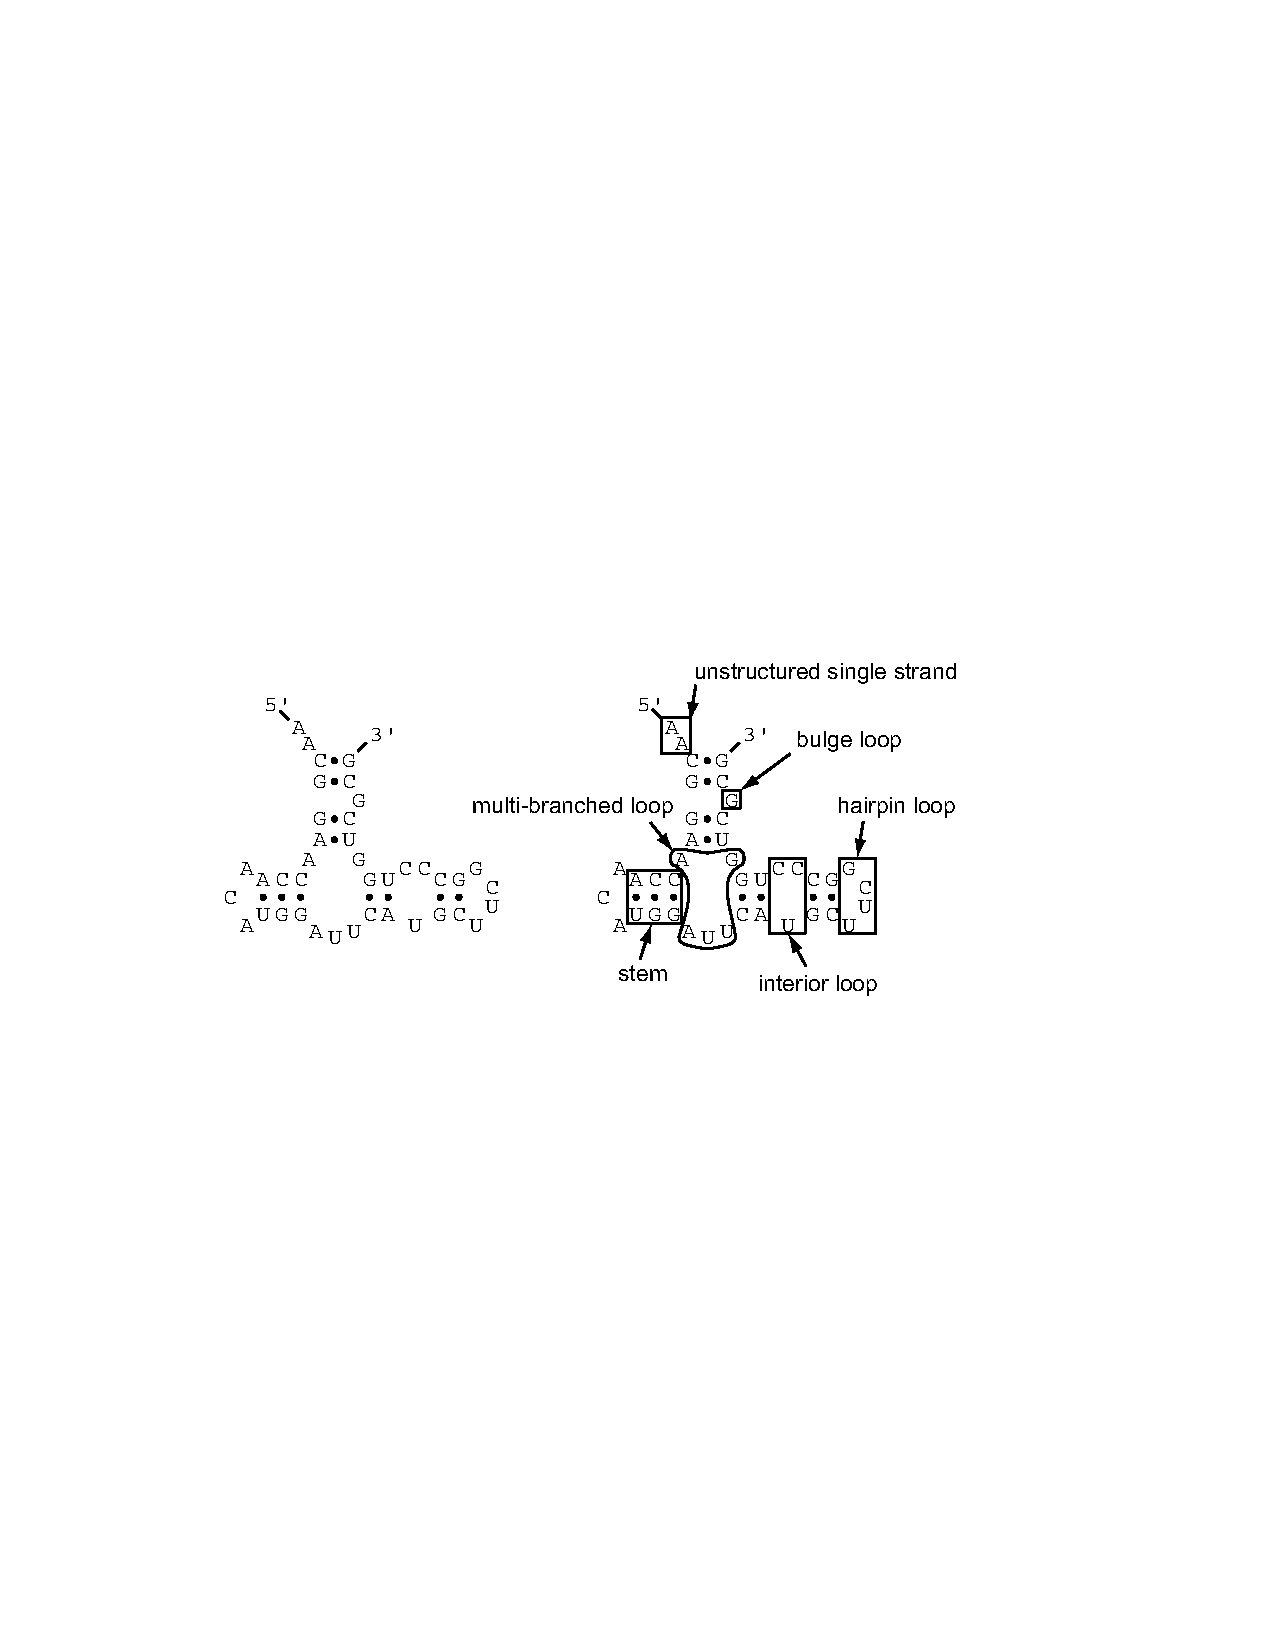
\includegraphics[scale=0.8]{figures/rna_elements}
\end{center}
\begin{center}
\begin{BVerbatim}
  ::((((,<<<___>>>,,,<<-<<____>>-->>,))-))
  AACGGAACCAACAUGGAUUCAUGCUUCGGCCCUGGUCGCG
\end{BVerbatim}
\end{center}

\subsection{Full (output) WUSS notation}

In detail, symbols used by WUSS notation in \emph{output} structure
annotation strings are as follows:

\begin{sreitems}{\textbf{Bulge, interior loops}}
\item[\textbf{Base pairs}]
  Base pairs are annotated by nested matching pairs of symbols
  \verb+<>+, \verb+()+, \verb+[]+, or \verb+{}+.
  The different symbols indicate the ``depth'' of the
  helix in the RNA structure as follows:
  \verb+<>+ are used for simple terminal stems;
  \verb+()+ are used for ``internal'' helices enclosing a multifurcation of
  all terminal stems; \verb+[]+ are used for internal helices
  enclosing a multifurcation that includes at least one annotated
  \verb+()+ stem already; and \verb+{}+ are used for all internal
  helices enclosing deeper multifurcations.

\item[\textbf{Hairpin loops}]
  Hairpin loop residues are indicated by underscores, \verb+_+.
  Simple stem loops stand out as, e.g.\ \verb+<<<<____>>>>+.

\item[\textbf{Bulge, interior loops}]
  Bulge and interior loop residues are indicated by dashes, \verb+-+.

\item[\textbf{Multifurcation loops}]
  Multifurcation loop residues are indicated by commas, \verb+,+.
  The mnemonic is ``stem 1, stem2'', e.g.\ \verb+<<<___>>>,,<<<___>>>+.

\item[\textbf{External residues}]
  Unstructured single stranded residues completely outside the
  structure (unenclosed by any base pairs) are annotated by
  colons, \verb+:+.

\item[\textbf{Insertions}]
  Insertions relative to a known structure are indicated by periods,
  \verb+.+. Regions where local structural alignment was invoked,
  leaving regions of both target and query sequence unaligned,
  are indicated by tildes, \verb+~+. These symbols only appear in
  alignments of a known (query) structure annotation to a target
  sequence of unknown structure.

\item[\textbf{Pseudoknots}]
  WUSS notation allows pseudoknots to be annotated as pairs of
  upper case/lower case letters: for example,
  \verb+<<<<_AAAA____>>>>aaaa+ annotates a simple pseudoknot;
  additional pseudoknotted stems could be annotated by \verb+Bb+,
  \verb+Cc+, etc. 

  This is not a fully general notation. It is possible to come up with
  pseudoknotted structures that could not be represented with 26
  levels of nesting ($>$26th order pseudoknot, in the sense of
  \citep{RivasEddy99}). However, it is unlikely you will ever see one
  in nature. I believe the highest order pseudoknot known is the S1
  (alpha operon) pseudoknot, which is 3rd order.
\end{sreitems}

An example of WUSS notation for a complicated structure
(\emph{E. coli} RNase P) is shown in Figure~\ref{fig:RNaseP}.  An
example of WUSS notation for a local alignment of \emph{B. subtilis}
RNase P to \emph{E. coli} RNase P, illustrating the use of local
alignment annotation symbols, is in Figure~\ref{fig:bsu-alignment}.

\begin{figure}[tp]
\begin{center}
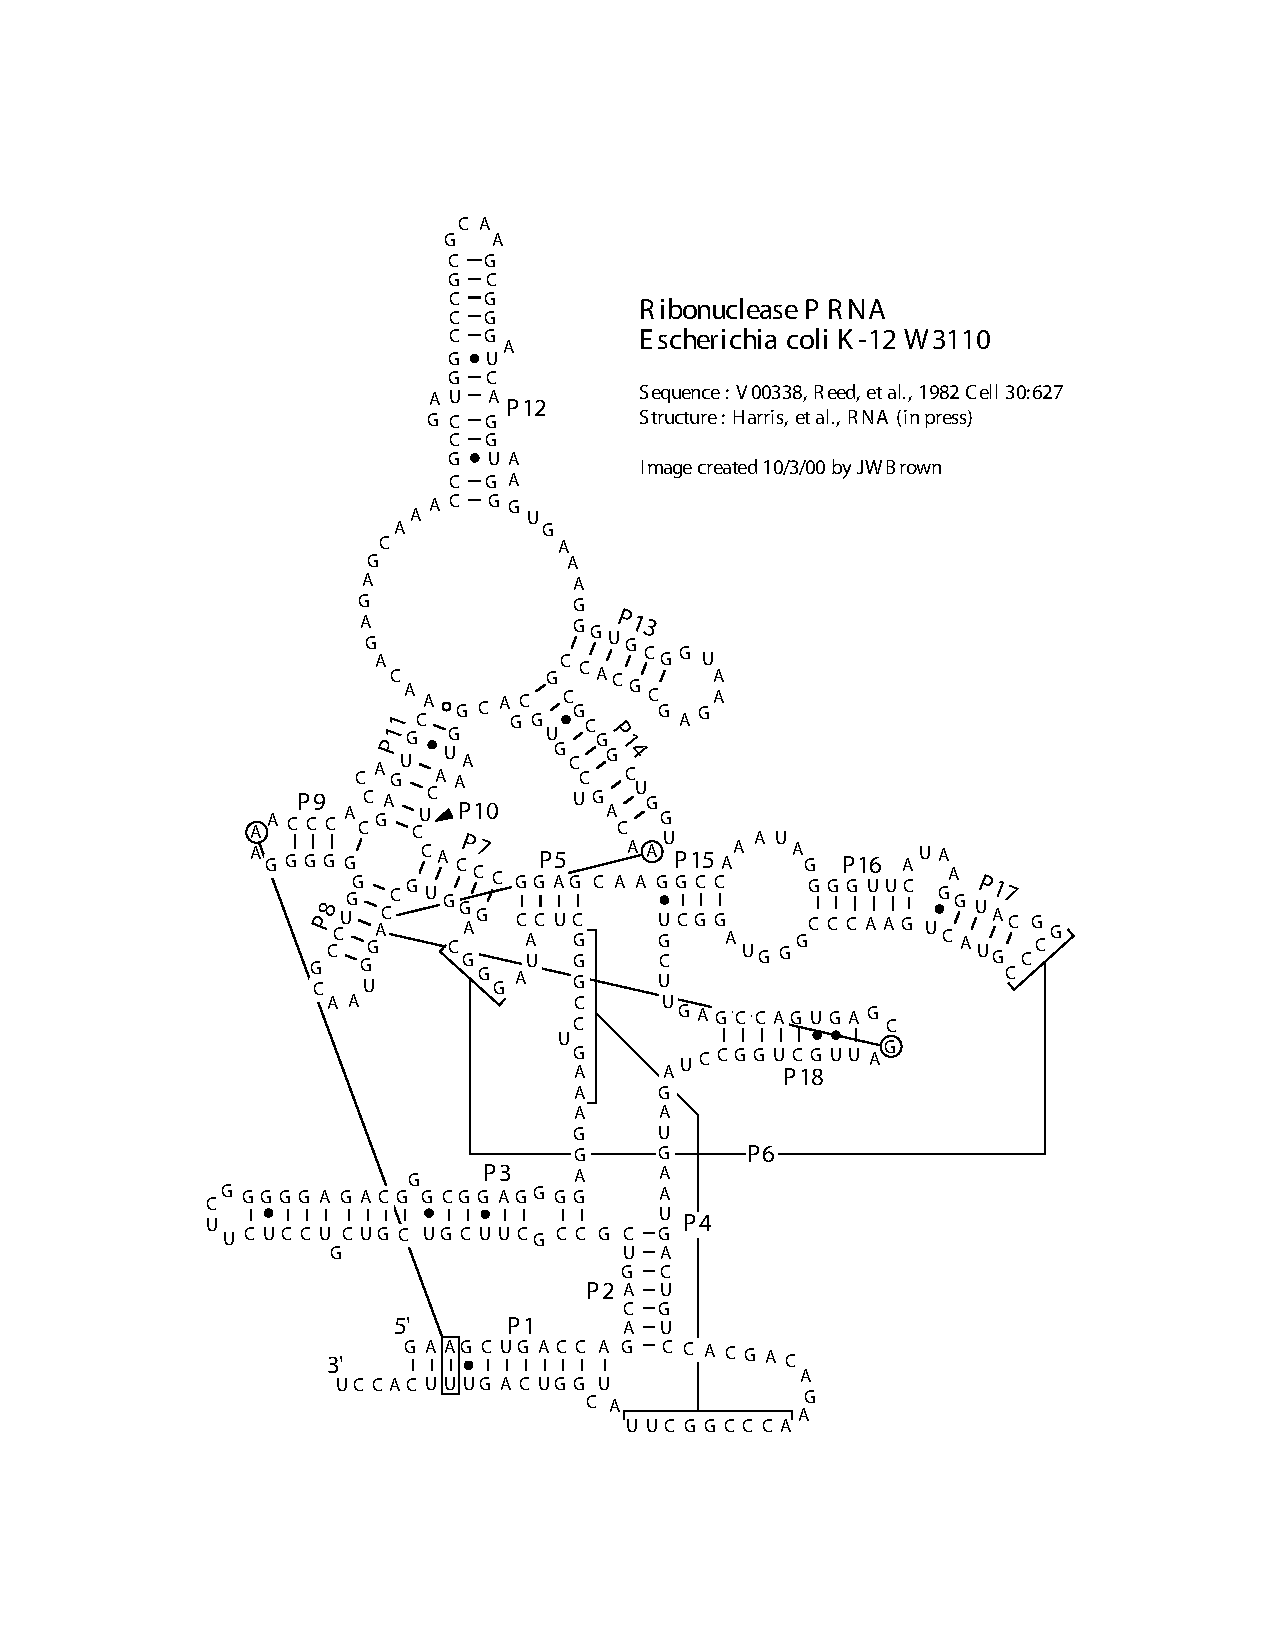
\includegraphics[scale=0.6]{figures/rnaseP-ecoli}
\end{center}
\begin{center}
{\scriptsize
\begin{BVerbatim}
           {{{{{{{{{{{{{{{{{{,<<<<<<<<<<<<<-<<<<<____>>>>>>>>>->>>>>>>>
         1 GAAGCUGACCAGACAGUCGCCGCUUCGUCGUCGUCCUCUUCGGGGGAGACGGGCGGAGGG 60

           >,,,,AAA-AAAAA[[[[---BBBB-[[[[[<<<<<_____>>>>><<<<____>>>->(
        61 GAGGAAAGUCCGGGCUCCAUAGGGCAGGGUGCCAGGUAACGCCUGGGGGGGAAACCCACG 120

           (---(((((,,,,,,,,,,,,<<<<<--<<<<<<<<____>>>>>->>>>>>-->>,,,,
       121 ACCAGUGCAACAGAGAGCAAACCGCCGAUGGCCCGCGCAAGCGGGAUCAGGUAAGGGUGA 180

           ,,,<<<<<<_______>>>>>><<<<<<<<<____>>>->>>>>->,,)))--))))]]]
       181 AAGGGUGCGGUAAGAGCGCACCGCGCGGCUGGUAACAGUCCGUGGCACGGUAAACUCCAC 240

           ]]]]]],,,<<<<------<<<<<<----<<<<<_bbbb>>>>>>>>>>>----->>>>,
       241 CCGGAGCAAGGCCAAAUAGGGGUUCAUAAGGUACGGCCCGUACUGAACCCGGGUAGGCUG 300

           ,,,,,<<<<<<<<____>>>>>>>>,,,,,,,,,,}}}}}}}----------aaaaaaaa
       301 CUUGAGCCAGUGAGCGAUUGCUGGCCUAGAUGAAUGACUGUCCACGACAGAACCCGGCUU 360

           -}-}}}}}}}}}}::::
       361 AUCGGUCAGUUUCACCU 377
\end{BVerbatim}
}
\end{center}
\caption{\small \textbf{Example of WUSS notation.} Top: Secondary
structure of \emph{E. coli} RNase P, from Jim Brown's RNase P database
\citep{Brown99}. Bottom: WUSS notation for the same structure,
annotating the \emph{E. coli} RNase P sequence. Note that the P4 and P6
pseudoknots are annotated, as A's and B's.}
\label{fig:RNaseP}
\end{figure}

\begin{figure}[tp]
\begin{center}
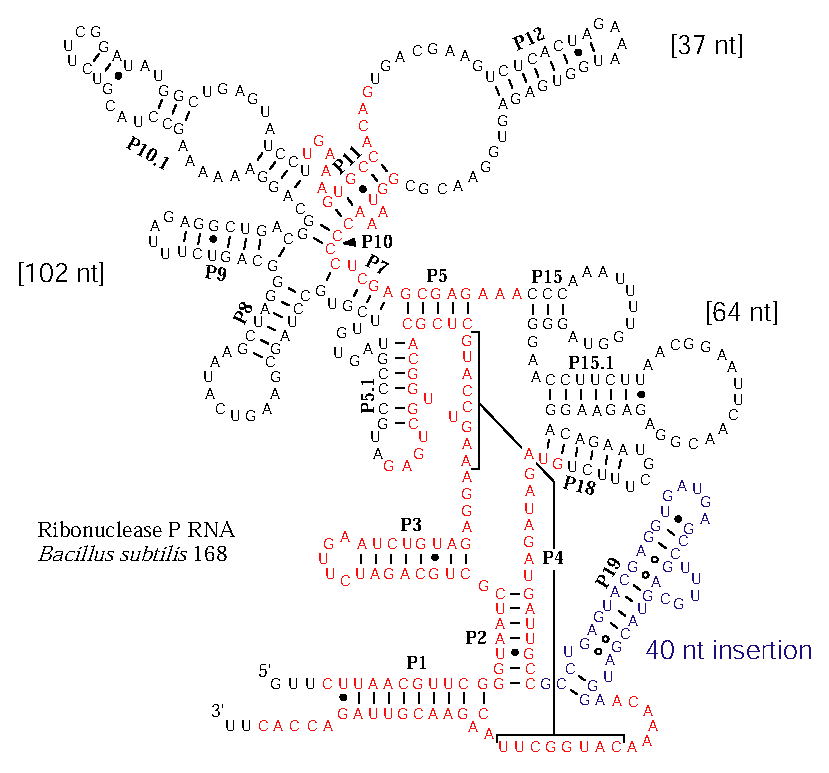
\includegraphics[scale=0.6]{figures/rnaseP-bsu-alignment}
\end{center}
\begin{center}
{\scriptsize
\begin{BVerbatim}
hit 0   :      4    399    52.56 bits
           {{{{{{{{{{{{{{{{{{,<<<<<<<<<<<<<-<<<<<____>>>>>>>>>->>>>>>>>
         1 ggAGuggGgcaGgCaguCGCugcuucggccuuGuucaguuaacugaaaaggAccgaagga 60
           +: :::G::C:GG:A:UCGCU+C::::            U+            ::::G+A
         4 CUUAACGUUCGGGUAAUCGCUGCAGAUC-----------UUG----------AAUCUGUA 42

           >,,,,,,,,,,,,,[[[.[--------[[[[[~~~~~~~((---(((((,,,,~~~~~~)
        61 GAGGAAAGUCCGGGCUC.CACAGGGCAgGGUG*[ 29]*GGAAAGUGCCACAG*[96]*G 229
           GAGGAAAGUCC  GCUC C  A GG   :G G       :GAAAGUGCCACAG      G
        43 GAGGAAAGUCCAUGCUCgC--ACGGUGCUGAG*[102]*UGAAAGUGCCACAG*[37]*G 226

           ))--))))]]]]]].]]],,,~~~~~~,,,,,,,,,,}}}}}}}--..............
       230 GUAAACCCCACCcG.GAGCAA*[77]*CuAGAUGAAUGacuGcCCA.............. 344
           GUAAACC:C C: G GAG AA       UAGAU++AUGA:U:CC
       227 GUAAACCCCUCGAGcGAGAAA*[64]*GUAGAUAGAUGAUUGCC--gccugaguacgagg 342

           ..........................-----------------}-}}}}}}}}}}::::
       345 ..........................CGACAGAACCCGGCUUAuagcCccaCUccucuu 377
                                       ACA AAC  GGCUUA:AG::C::: :+ C
       343 ugaugagccguuugcaguacgaugga--ACAAAACAUGGCUUACAGAACGUUAGACCAC 399
\end{BVerbatim}
}
\end{center}
\caption{\small \textbf{Local alignment annotation example.} Top:
Secondary structure of \emph{B. subtilis} RNase P, from Jim Brown's
RNase P database \citep{Brown99}. Residues in red are those that
Infernal aligns to a CM of \emph{E. coli} type RNase
P's. The local structural alignment is in four pieces; three regions
of the structure (102, 37, and 64 nt long) are skipped over. One
additional stem is treated as a 40 nt insertion. Bottom: the
Infernal output, showing the \emph{E. coli} query structure
aligned to the \emph{B. subtilis} sequence.}
\label{fig:bsu-alignment}
\end{figure}

\subsection{Shorthand (input) WUSS notation}

While WUSS notation makes it easier to visually interpret Infernal
\emph{output} structural annotation, it would be painful to require
people to \emph{input} all structures in full WUSS notation. Therefore
when software like Infernal reads input secondary structure
annotation, it also allows simpler rules:

\begin{sreitems}{\textbf{Single stranded residues}}
\item [\textbf{Base pairs}]
  Any matching nested pair of \verb+()+, \verb+()+, \verb+[]+, \verb+{}+
  symbols indicates a base pair; the exact choice of symbol has no
  meaning, so long as the left and right partners match up.
  Similarly, pseudoknotted pairs can also be annotated by matching nested
  pairs of any alphabet character, such as \verb+Aa+, \verb+Bb+, etc.

\item [\textbf{Single stranded residues}]
  All other symbols \verb+_-,:.~+
  indicate single stranded residues.
  The choice of symbol has no special meaning.
  Annotated pseudoknots (nested matched pairs of upper/lower case
  alphabetic characters) are also interpreted as single
  stranded residues in Infernal input.
\end{sreitems}

Thus, for instance, \verb+<<<<....>>>>+ and \verb+((((____))))+ and
\verb+<(<(._._)>)>+ all indicate a four base stem with a four base
loop (the last example is legal but weird).

Remember that the key property of canonical (nonpseudoknotted) RNA
secondary structure is that the pairs are \emph{nested}.
\verb+((<<....))>>+ is not a legal annotation string: the pair symbols
don't match up properly. 

Because many other RNA secondary structure analysis programs use a
simple bracket notation for annotating structure, the ability to input
the simple format makes it easier to use data generated by other RNA
software packages. Conversely, converting output WUSS notation to
simple bracket notation is a matter of a simple Perl or sed script,
substituting the symbols appropriately.

}{}

\ifthenelse{\boolean{completedraft}}{
\newpage
\section{NCBI BLAST database foramt}

The NCBI BLAST databases are generated by the program \emph{formatdb}.
The three files needed by Easel are index file, sequence file 
and header file.For protein databases these files end with the extension 
".pin", ".psq" and ".phr" respectively.  For DNA databases the 
extensions are ".nin", ".nsq" and ".nhr" respectively.  The index 
file contains information about the database, i.e. version number, 
database type, file offsets, etc.  The sequence file contains residues
for each of the sequences.  Finally, the header file contains the header 
information for each of the sequences.  This document describes the
structure of the NCBI version 4 database.

If these files cannot be found, an alias file, extensions ".nal" or
 ".pal", is processed.  The alias file is used to specify multiple
volumes when databases are larger than 2 GB.


\subsection{Index File (*.pin, *.nin)}

The index file contains format information about the database.   The 
layout of the version 4 index file is below:

\bigskip
\begin{center}
\begin{tabular}{|l|l|p{3.5in}|} \hline
Version &
Int32 &
Version number. \\ \hline
Database type &
Int32 &
0-DNA 1-Protein.  \\ \hline
Title length &
Int32 &
Length of the title string (\emph{T}).  \\ \hline
Title &
Char[\emph{T}] &
Title string.  \\ \hline
Timestamp length &
Int32 &
Length of the timestamp string (\emph{S}).  \\ \hline
Timestamp &Char[\emph{S}] &
Time of the database creation.  The length of the timestamp \emph{S} is 
increased to force 8 byte alignment of the remaining integer 
fields.  The timestamp is padded with NULs to achieve this alignment.   \\ \hline
Number of sequences &
Int32 &
Number of sequences in the database (\emph{N})  \\ \hline
Residue count &
Int64 &
Total number of residues in the database.  Note:  Unlike other integer 
fields, this field is stored in little endian.  \\ \hline
Maximum sequence &
Int32 &
Length of the longest sequence in the database  \\ \hline
Header offset table &
Int32[\emph{N+1}] &
Offsets into the sequence's header file (*.phr, *nhr). \\ \hline
Sequence offset table &
Int32[\emph{N+1}] &
Offsets into the sequence's residue file (*.psq, *.nsq). \\ \hline
Ambiguity offset table &
Int32[\emph{N+1}] &
Offset into the sequence's residue file (*.nsq).  Note: This table is only 
in DNA databases.  If the sequence does not have any ambiguity 
residues, then the offset points to the beginning of the next 
sequence.  \\ \hline
\end{tabular}
\end{center}
\bigskip

The integer fields 
are stored in big endian format, except for the residue count which is 
stored in little endian.  The two string fields, timestamp and title 
are preceded by a 32 bit length field.  The title string is not NUL 
terminated.  If the end of the timestamp field does not end on an offset 
that is a multiple of 8 bytes, NUL characters are padded to the end of 
the string to bring it to a multiple of 8 bytes.  This forces all the 
following integer fields to be aligned on a 4-byte boundary for 
performance reasons.  The length of the timestamp field reflects the 
NUL padding if any.  The header offset table is a list of offsets to
the beginning of each sequence's header.  These are offsets into
the header file (*.phr, *.nhr).  The size of the header can be 
calculated by subtracting the offset of the next header from the 
current header.  
The sequence offset table is a list of offsets to
the beginning of each sequence's residue data.  These are offsets into
the sequence file (*.psq, *.nsq).  The size of the sequence can be 
calculated by subtracting the offset of the next sequence from the 
current sequence.  
Since one more offset is stored than the number 
of sequences in the database, no special code is needed in calculating 
the header size or sequence size for the last entry in the database.


\subsection{Protein Sequence File (*.pin)}

The sequence file contains the sequences, one after another.  The 
sequences are in a binary format separated by a NUL byte.  Each 
residue is encoded in eight bits.

\bigskip
\begin{center}
\begin{tabular}{|c|c|c|c|c|c|c|c|} \hline
Amino acid & Value & Amino acid & Value & Amino acid & Value & Amino acid & Value \\ \hline
- & 0 & G &  7 & N & 13 & U & 24 \\ \hline
A & 1 & H &  8 & O & 26 & V & 19 \\ \hline
B & 2 & I &  9 & P & 14 & W & 20 \\ \hline
C & 3 & J & 27 & Q & 15 & X & 21 \\ \hline
D & 4 & K & 10 & R & 16 & Y & 22 \\ \hline
E & 5 & L & 11 & S & 17 & Z & 23 \\ \hline
F & 6 & M & 12 & T & 18 & * & 25 \\ \hline
\end{tabular}
\end{center}


\subsection{DNA Sequence File (*.nsq)}

The sequence file contains the sequences, one after another.  The 
sequences are in a binary format but unlike the protein sequence 
file, the sequences are not separated by a NUL byte.  The 
sequence is first compressed using two bits per residue then 
followed by an ambiguity correction table if 
necessary.  If the sequence does not have an ambiguity table, 
the sequence's ambiguity index points to the beginning of the 
next sequence.

\subsubsection{Two-bit encoding}

The sequence is encoded first using two bits per nucleotide.

\bigskip
\begin{center}
\begin{tabular}{|c|c|c|} \hline
Nucleotide & Value & Binary \\ \hline
A & 0 & 00 \\ \hline
C & 1 & 01 \\ \hline
G & 2 & 10 \\ \hline
T or U & 3 & 11 \\ \hline
\end{tabular}
\end{center}
\bigskip

Any 
ambiguous residues are replaced by an 'A', 'C', 'G' or 'T' in 
the two bit encoding.  To calculate the number of residues 
in the sequence, the least significant two bits in the 
last byte of the sequence needs to be examined.  
These last two bits indicate how many residues, if any, are 
encoded in the most significant bits of the last byte.


\subsubsection{Ambiguity Table}

To correct a sequence containing any degenerate residues, an 
ambiguity table follows the two bit encoded string.  
The start of the ambiguity table is 
pointed to by the ambiguity table index in the index file, 
"*.nin".  The first four bytes contains the number of 32 bit 
words in the correction table.  If the most significant bit 
is set in the count, then two 32 bit entries will be used for 
each correction.  
The 64 bit entries are used for sequence with
more than 16 million residues.  Each correction contains three 
pieces of 
information, the actual encoded nucleotide, how many nucleotides
in the sequence are replaced by the correct nucleotide and finally 
the offset into the sequences to apply the correction. 

For 32 bit
entries, the first 4 most significant bits encodes the nucleotide.
Their bit pattern is 
true of their representation, i.e. the value of 'H' is equal 
to ('A'~or~'T'~or~'C').  

\bigskip
\begin{center}
\begin{tabular}{|c|c|c|c|c|c|c|c|} \hline
Nucleotide & Value & Nucleotide & Value & Nucleotide & Value & Nucleotide & Value \\ \hline
- & 0 & G & 4 & T & 8  & K & 12 \\ \hline
A & 1 & R & 5 & W & 9  & D & 13 \\ \hline
C & 2 & S & 6 & Y & 10 & B & 14 \\ \hline
M & 3 & V & 7 & H & 11 & N & 15 \\ \hline
\end{tabular}
\end{center}
\bigskip

The next field is the repeat count which is four bits wide. 
One is added to the count giving it the range of 1 -- 256.  
The last 24 bits is the offset into the sequence where the
replacement starts.  The first residue start at offset zero,
the second at offset one, etc.  With a 24 bit size, the offset
can only address sequences around 16 million residues long.

To address larger sequences, 64 bit
entries are used.  For 64 bit entries, the order of the entries stays the same, 
but their sizes change.  The nucleotide remains at four bits.
The repeat count is increased to 12 bits giving it the range 
of 1 -- 4096.  The offset size is increased to 48 bits.


\subsection{Header File (*.phr, *.nhr)}

The header file contains the headers for each sequence, one after another.  
The sequences are in a binary encoded ASN.1 format.  The length 
of a header can be calculated by subtracting the offset of the 
next sequence from the current sequence offset.  The ASN.1 definition 
for the headers can be found in the NCBI toolkit in the following 
files: asn.all and fastadl.asn.

The parsing of the header can be done with a simple recursive 
descent parser.  The five basic types defined in the header are:

\begin{itemize}
\item Integer -- a variable length integer value.
\item VisibleString -- a variable length string.
\item Choice -- a union of one or more alternatives.  
\item Sequence -- an ordered collection of one or more types.  
\item SequenceOf -- an ordered collection of zero or more occurrences 
of a given type.
\end{itemize} 

\subsubsection{Integer}

The first byte of an encoded integer is a hex \verb+02+.  The next byte 
is the number of bytes used to encode the integer value.  The 
remaining bytes are the actual value.  The value is encoded 
most significant byte first.

\subsubsection{VisibleString}

The first byte of a visible string is a hex \verb+1A+.  
The next byte 
starts encoding the length of the string.  If the most 
significant bit is off, then the lower seven bits encode the 
length of the string, i.e. the string has a length less than 128. 
If the most significant bit is on, then 
the lower seven bits is the number of bytes that hold the length of 
the string, then the bytes encoding the string length, most significant 
bytes first.
Following the length are the actual string characters.
The strings are not NUL terminated.  

\subsubsection{Choice}


The first byte indicates which selection of the choice.  The choices 
start with a hex value \verb+A0+ for the first item, \verb+A1+ for 
the second, etc.  
The selection is followed by a hex \verb+80+.  Two NUL bytes follow 
the choice.

\subsubsection{Sequence}

The first two bytes are a hex \verb+3080+.  The header is 
then followed by 
the encoded sequence types.  The first two bytes indicates which type 
of the sequence is encoded.  This index starts with the hex value 
\verb+A080+ 
for the first item, \verb+A180+ for the second, etc. then 
followed by the 
encoded item and finally two NUL bytes, \verb+0000+, to indicate the end 
of that type.  The next type in the sequence is then encoded.  If an 
item is optional and is not defined, then none of it is encoded 
including the index and NUL bytes.  This is repeated until the entire 
sequence has been encoded.  Two NUL bytes then mark the end of the 
sequence.

\subsubsection{SequenceOf}

The first two bytes are a hex \verb+3080+.  Then the lists of objects are 
encoded.  Two NUL bytes encode the end of the list.

}{}

\ifthenelse{\boolean{completedraft}}{
\newpage
%%%%%%%%%%%%%%%%%%%%%%%%%%%%%%%%%%%%%%%%%%%%%%%%%%%%%%%%%%%%%%%%
   \chapter{Developer's guide}

\begin{quote}
   \emph{This is the great nightmare, when you're doing something long
     and hard, is you're terrified that it will be perceived as
     gratuitously hard and difficult, that it is some
     avant-garde-for-its-own-sake kind of exercise.}\\
   \hspace*{1em}\hfill -- David Foster Wallace, speaking of \emph{Infinite Jest}
\end{quote}

   
This chapter describes Easel from a developer's perspective. It shows
how a module's source code is organized, written, tested, and
documented. It should help you with implementing new Easel code, and
also with understanding the structure of existing Easel code.

We expect Easel to constantly evolve, both in code and in style.
Talking about our code style does not mean we enforce foolish
consistency. Rather, the goal is aspirational; one way we try to
manage the complexity of our growing codebase is to continuously
cajole Easel code toward a clean and consistent presentation. We try
to organize code modules in similar ways, use certain naming
conventions, and channel similar functions towards common
\esldef{interfaces} that provide common calling conventions and
behaviors.

But because it evolves, not all Easel code obeys the code style
described in this chapter. Easel code style is like a local building
ordinance. Any new construction should comply. Older construction is
grandfathered in and does not have to immediately conform to the
current rules. When it comes time to renovate, it's also time to bring
the old work up to the current standards.

For a concrete example we will focus primarily on one Easel module,
the \eslmod{buffer} module. We'll take a bottom up approach, starting
from the overall organization of the module and working down into
details. If you're a starting developer, you might have preferred a
bottom-up description; you might just want to know how to write or
improve a single Easel function, for example. In that case, skim
ahead.

%%%%%%%%%%%%%%%%%%%%%%%%%%%%%%%%%%%%%%%%%%%%%%%%%%%%%%%%%%%%%%%%
% Table: Easel naming conventions
%%%%%%%%%%%%%%%%%%%%%%%%%%%%%%%%%%%%%%%%%%%%%%%%%%%%%%%%%%%%%%%%
\begin{table}
\begin{minipage}{\textwidth}
\begin{tabular}{l>{\raggedright}p{3.5in}l}
\textbf{What}        & \textbf{Explanation}              & \textbf{Example} \\ \hline
Easel module
  &
    Module names should be 10 characters or less.\footnote{sqc assumes
    this in output formatting, for example.}
    Many modules are organized around a single Easel object
    that they implement. The name of the module matches the
    name of the object. For example, \ccode{esl\_buffer.c} implements \ccode{ESL\_BUFFER}.
  & \eslmod{buffer} \\ \\

tag name
  & Names in the module are constructed either using the module's full
    name or sometimes with a shorter abbreviation, usually 3
    characters (sometimes 2 or 4).
  & \ccode{buf} \\ \\

source file
  & Each module has one source file, named \ccode{esl\_}\itcode{modulename}\ccode{.c}.
  & \ccode{esl\_buffer.c} \\ \\

header file
  & Each module has one header file, named \ccode{esl\_}\itcode{modulename}\ccode{.h}.
  & \ccode{esl\_buffer.h} \\  \\

documentation 
  & Each module has one documentation chapter, named \ccode{esl\_}\itcode{modulename}\ccode{.tex}.
  & \ccode{esl\_buffer.tex} \\ \\

Easel object          
  & Easel ``objects'' are typedef'ed C structures (usually) or
    types (rarely\footnote{\ccode{ESL\_DSQ} is a \ccode{uint8\_t}, for example.}).
  & \ccode{ESL\_BUFFER} \\ \\  

external function 
  & All exposed functions have tripartite names \ccode{esl\_}\itcode{module}\ccode{\_specificname}().
    The specific part of function names often adhere to a standardized API
    ``interface'' nomenclature. (All \ccode{\_Open()} functions must follow the same standardized
    behavior guidelines, for example.) Functions in the base \ccode{easel.c} module
    have a bipartite name, omitting the module name. The specific 
    name part generally uses mixed case capitalization.
  & \ccode{esl\_buffer\_OpenFile()} \\ \\

static function 
  & Internal functions (static within a module file) drop the
    \ccode{esl\_} prefix, and are 
    named \itcode{modulename}\ccode{\_function}.
  & \ccode{buffer\_refill()} \\ \\

macro 
  & Macros follow the same naming convention as external functions,
    except they are all upper case.
  & \ccode{ESL\_ALLOC()} \\ \\ 

defined constant
  & Defined constants in Easel modules are named
    \ccode{esl}\itcode{MODULENAME}\ccode{\_FOO}. Constants defined
    in the base \ccode{easel.h} module are named just 
    \ccode{eslFOO}.
   & \ccode{eslBUFFER\_SLURPSIZE}\\ \\

return codes
  & Return codes are constants defined in \ccode{easel.h}, so 
    they obey the rules of other defined constants in the base module (\ccode{eslOK},
    \ccode{eslFAIL}). Additionally, error codes start with
    \ccode{E}, as in \ccode{eslE}\itcode{ERRTYPE}.
  & \ccode{eslENOTFOUND} \\ \\

config constant
  & Constants that don't start with \ccode{esl} are almost always 
    configuration (compile-time) constants determined by the autoconf
    \ccode{./configure} script and defined in \ccode{esl\_config.h}.
  & \ccode{HAVE\_STDINT\_H} \\ \\
\end{tabular}
\end{minipage}
\caption{\textbf{Easel naming conventions.} }
\end{table}



%%%%%%%%%%%%%%%%%%%%%%%%%%%%%%%%%%%%%%%%%%%%%%%%%%%%%%%%%%%%%%%%
\section{An Easel module}
%%%%%%%%%%%%%%%%%%%%%%%%%%%%%%%%%%%%%%%%%%%%%%%%%%%%%%%%%%%%%%%%

Each module consists of three files: a .c C code file, a .h header
file, and a .tex documentation file. These filenames are constructed
from the module name. For example, the \eslmod{buffer} module is
implemented in \ccode{esl\_buffer.c}, \ccode{esl\_buffer.h}, and
\ccode{esl\_buffer.tex}.

%%%%%%%%%%%%%%%%
\subsection{The .c file}
%%%%%%%%%%%%%%%%

Easel \ccode{.c} files are larger than most coding styles would
advocate. Easel module code is designed to be \emph{read}, to be
\emph{self-documenting}, to contain its own \emph{testing methods},
and to provide useful \emph{working examples}.  Thus the size of the
files is a little deceptive, compared to C code that's solely
implementating some functions. In general, only about a a quarter of
an Easel module's \ccode{.c} file is the actual module implementation.
Typically, around half of an Easel \ccode{.c} file is documentation,
and much of this gets automatically parsed into the PDF userguide. The
rest consists of drivers for unit testing and examples.

Module files are organized into a somewhat stereotypical set of
sections, to facilitate navigating the code, as follows.

The \ccode{.c} file starts with a comment that contains the {\bfseries
  table of contents}. The table of contents helps us navigate a long
Easel source file. This initial comment also includes a short
description of the module's purpose. It may also contain miscellaneous
notes.

For example, from the \eslmod{buffer} module:

\begin{cchunk}
/* An input parsing abstraction.
 *
 * Table of contents:
 *   1. ESL_BUFFER object: opening/closing.
 *   2. Positioning and anchoring an ESL_BUFFER.
 *   3. Raw access to the buffer.
 *   4. Line-based parsing.
 *   5. Token-based parsing.
 *   6. Binary (fread-like) parsing.
 *   7. Private (static) functions.
 *   8. Benchmark.
 *   9. Unit tests.
 *  10. Test driver.
 *  11. Examples.
 */
\end{cchunk}


None of this is parsed automatically. Its structure is just
convention.

The short description lines in the table of contents match section
headings in comments later in the file. A search forward with the text
of a heading will move you to that section of the code.

Next come the {\bfseries includes} and any {\bf definitions}. Of the
include files, the \ccode{esl\_config.h} header must always be
included first. It contains platform-independent configuration code
that may affect even the standard library header files. Standard
headers like \ccode{stdio.h} come next, then Easel's main header
\ccode{easel.h}; then headers of any other Easel modules this module
depends on, then the module's own header. For example, the
\ccode{\#include}'s in the \eslmod{buffer} module look like:

\begin{cchunk}
#include "esl_config.h"

#include <stdio.h>
#include <stdlib.h>
#include <string.h>
#include <signal.h>   // one of the utests uses alarm() to catch an infinite loop bug

#ifdef HAVE_UNISTD_H
#include <unistd.h>
#endif
#ifdef _POSIX_VERSION
#include <fcntl.h>
#include <sys/mman.h>
#include <sys/stat.h>
#endif /* _POSIX_VERSION */

#include "easel.h"
#include "esl_mem.h"

#include "esl_buffer.h"
\end{cchunk}


Next come the {\bfseries private function declarations}.  We declare
all private functions at the top of the file, where they can be seen
easily by a developer who's casually reading the source. Their
definitions are buried deeper, in one or more sections following the
implementation of the exposed API.

\begin{cchunk}
static int buffer_create           (ESL_BUFFER **ret_bf);
static int buffer_init_file_mmap   (ESL_BUFFER *bf, esl_pos_t filesize);
static int buffer_init_file_slurped(ESL_BUFFER *bf, esl_pos_t filesize);
static int buffer_init_file_basic  (ESL_BUFFER *bf);

static int buffer_refill   (ESL_BUFFER *bf, esl_pos_t nmin);
static int buffer_countline(ESL_BUFFER *bf, esl_pos_t *opt_nc, esl_pos_t *opt_nskip);
static int buffer_skipsep  (ESL_BUFFER *bf, const char *sep);
static int buffer_newline  (ESL_BUFFER *bf);
static int buffer_counttok (ESL_BUFFER *bf, const char *sep, esl_pos_t *ret_nc);
\end{cchunk}


The rest of the file is the {\bfseries code}. It is split into
sections. Each section is numbered and given one-line titles that
appear in the table of contents.  Each section starts with a section
header, a comment block in front of each code section in the
\ccode{.c} file.  These section headers match comments in front of
that section's declarations in the \ccode{.h} file. Because of the
numbering and titling, a particular section of code can be located by
searching on the number or title.  A common section structure includes
the following, in this order:


\begin{description}
\item[\textbf{The \ccode{FOOBAR} object.}]
  The first section of the file provides the API for creating and
  destroying the object that this module implements.

\item[\textbf{The rest of the API.}]
  Everything else that is part of the API for this module.
  This might be split across multiple sections.

\item[\textbf{Debugging/dev code.}]
  Most objects can be validated or dumped to an output stream
  for inspection.

\item[\textbf{Private functions.}]
  Easel isn't rigorous about where private (non-exposed) functions go,
  but they often go in a separate section in about the middle of the
  \ccode{.c} file, after the API and before the drivers.

\item[\textbf{Optional drivers}] Stats, benchmark, and regression
  drivers, if any. 

\item [\textbf{Unit tests.}]
  The unit tests are internal controls that test that the module's API
  works as advertised.

\item [\textbf{Test driver.}]
  All modules have an automated test driver is a \ccode{main()} that
  runs the unit tests.
 
\item [\textbf{Examples.}]
  All modules have at least one \ccode{main()} showing an example of
  how to use the main features of the module.

\end{description}

%%%%%%%%%%%%%%%%
\subsection{The .h file}
%%%%%%%%%%%%%%%%


%%%%%%%%%%%%%%%%
\subsection{Special syntax in Easel C comments}
%%%%%%%%%%%%%%%%

Easel comments sometimes include special syntax recognized by tools other
than the compiler.  Here are some quick explanations of the special
stuff a developer needs to be aware of. 

\begin{table}
\begin{tabular}{l>{\raggedright}p{3.5in}l}
\textbf{Special syntax}  & \textbf{Description}  & \textbf{Parsed by}\\ \hline

\ccode{/* Function: }\itcode{funcname} 
  & Function documentation that gets converted to \LaTeX\ and included
    in Easel's PDF documentation.
  & \emcode{autodoc} \\ \\

\ccode{ *\# }\itcode{x.\ secheading} 
  & Section heading corresponding to section number x in a \ccode{.c}
    file's table of contents. This is automatically extracted as part
    of creating a summary table in the PDF documentation.
  & \emcode{autodoc -t} \\ \\

\ccode{/*::cexcerpt::} ...
  & Comments that marking beginning/end of code that is extracted
    verbatim into the documentation.
  & \emcode{cexcerpt} \\ \\

\hline
\end{tabular}
\caption{{\bfseries Summary of special syntax in Easel C comments.}}
\end{table}

%%%%
\subsubsection{function documentation}
%%%%

Any comment that starts with
\begin{cchunk}
/* Function:  ...
\end{cchunk}
will be recognized and parsed by our \prog{autodoc} program, 
which assumes it is looking at a structured function documentation
header.

See section XX for details on how these headers work.

We want all external functions in the Easel API to be documented
automatically by \prog{autodoc}. We don't want internal functions tp
appear in the documentation, but we do want them documented in the
code.  To keep \prog{autodoc} from recognizing the function header of
an internal (static) function, we just leave off the \ccode{Function:}
tag in the comment block.   

%%%%
\subsubsection{section headings}
%%%%

The automatically generated \LaTeX\ code for a module's documentation
includes a table summarizing the functions in the exposed API. This
table is constructed automatically from the source code by
\prog{autodoc -t}. The list of functions in this table is extracted
from the function documentation (above). The table is broken into
sections, just as the module code is, using section headings. The
comment block marking the start of a section heading for exposed API
code has an extra \ccode{\#}:

\begin{cchunk}
/*****************************************************************
 *# 1. ESL_BUFFER object: opening/closing.
 *****************************************************************/
\end{cchunk}

Section headings for internal functions omit the \ccode{\#}, and
\prog{autodoc} ignores them:

\begin{cchunk}
/*****************************************************************
 * 10. Unit tests
 *****************************************************************/
\end{cchunk}

%%%%
\subsubsection{excerpting}
%%%%

This book includes many examples of C code extracted verbatim from
Easel source.  These {\bfseries excerpts} are marked with specially
formatted comments in the C file:

\begin{cchunk}
/*::cexcerpt::my_example::begin::*/
   while (esl_sq_Read(sqfp, sq) == eslOK)
     { n++; }
/*::cexcerpt::my_example::end::*/
\end{cchunk}

When we build the Easel documentation from its source, our
\prog{cexcerpt} program extracts all marked excerpts from \ccode{.c}
and \ccode{.h} files, and places them in individual files in a
temporary \ccode{cexcerpts/} directory, from where they are included
in the main \LaTeX documentation.



%%%%%%%%%%%%%%%%
\subsection{Driver programs}
%%%%%%%%%%%%%%%%

An unusual (innovative?) thing about Easel modules is how we embed
{\bfseries driver programs} directly in the module's \ccode{.c}
file. Driver programs include our unit tests, benchmarks, and working
examples. These small programs are enclosed in standardized
\ccode{\#ifdef}'s that enable them to be conditionally compiled.

None of these programs are installed by \ccode{make install}.  Test
drivers are compiled as part of \ccode{make check}.  A \ccode{make
  dev} compiles all driver programs.

There are six main types of drivers used in Easel:

\begin{description} 

\item[\textbf{Unit test driver(s).}] (Mandatory.) Each module has one (and only one)
  \ccode{main()} that runs the unit tests and any other automated for
  the module. The test driver is compiled and run by the testsuite in
  \ccode{testsuite/testsuite.sqc} when one does a \ccode{make check}
  on the package. It is also run by several of the automated tools
  used in development, including the coverage (\ccode{gcov}) and
  memory (\ccode{valgrind}) tests. A test driver takes no arguments
  (it must generate any input files it needs). If it succeeds, it
  returns 0, with no output. If it fails, it returns nonzero and calls
  \ccode{esl\_fatal()} to issue a short error message on
  \ccode{stdout}. Our test harness, \emcode{sqc}, depends on these
  output and exit status conventions. Optionally, it may use a flag
  to show more useful output when it's run more interactively.
  (usually a \ccode{-v}, for verbose).
  The test driver is enclosed by
  \ccode{\#ifdef esl}\itcode{MODULE}\ccode{\_TESTDRIVE} for
  conditional compilation.

\item[\textbf{Regression/comparison test(s).}] (Optional.) These tests
  link to one or more libraries that provide identical comparable
  functionality, such as previous versions of Easel, the old
  \prog{SQUID} library, \prog{LAPACK} or the GNU Scientific Library.
  They test that Easel's functionality performs at least as it used
  to, or as well as the 'competition'. These tests are run on demand,
  and not included in automated testing, because the other libraries
  may only be present on a subset of our development machines. They
  are enclosed by \ccode{\#ifdef
    esl}\itcode{MODULE}\ccode{\_REGRESSION} for conditional
  compilation.

\item[\textbf{Benchmark(s).}] (Optional.) These tests run a
  standardized performance benchmark and collect time and/or memory
  statistics. They may generate output suitable for graphing. They are
  run on demand, not by automated tools. They typically use 
  \eslmod{stopwatch} for timing. They are enclosed by
  \ccode{\#ifdef esl}\itcode{MODULE}\ccode{\_BENCHMARK}  for
  conditional compilation.

\item[\textbf{Statistics generator(s).}] (Optional.) These tests collect
  statistics used to characterize the module's scientific performance,
  such as its accuracy at some task. They may generate graphing
  output. They are run on demand, not by automated tools. They are
  enclosed by \ccode{\#ifdef esl}\itcode{MODULE}\ccode{\_STATS}
  for conditional compilation.

\item[\textbf{Experiment(s).}] (Optional.) These are other reproducible
  experiments we've done on the module code, essentially the same as
  statistics generators. They are
  enclosed by \ccode{\#ifdef esl}\itcode{MODULE}\ccode{\_EXPERIMENT}
  for conditional compilation.

\item[\textbf{Example(s).}] (Mandatory). Every module has at least one example
  \ccode{main()} that provides a ``hello world'' level example of
  using the module's API. Examples are enclosed in \ccode{cexcerpt}
  tags for extraction and verbatim inclusion in the documentation.
  They are enclosed by \ccode{\#ifdef esl}\itcode{MODULE}\ccode{\_EXAMPLE} 
  for conditional compilation.
\end{description}  

All modules have at least one test driver and one example. Other tests
and examples are optional. When there is more than one \ccode{main()}
of a given type, the additional tags are numbered starting from 2: for
example, a module with three example \ccode{main()'s} would have three
tags for conditional compilation, \ccode{eslFOO\_EXAMPLE},
\ccode{eslFOO\_EXAMPLE2}, and \ccode{eslFOO\_EXAMPLE3}.

The format of the conditional compilation tags for all the drivers
(including test and example drivers) must be obeyed. Some test scripts
are scanning the .c files and identifying these tags
automatically. For instance, the driver compilation test identifies any
tag named
\ccode{esl}\itcode{MODULENAME}\ccode{\_\{TESTDRIVE,EXAMPLE,REGRESSION,BENCHMARK,STATS\}*}
and attempt to compile the code with that tag defined.

Which driver is compiled (if any) is controlled by conditional
compilation of the module's \ccode{.c} file with the appropriate
tag. For example, to compile and run the \eslmod{sqio} test driver as
a standalone module:

\begin{cchunk}
   %  gcc -g -Wall -I. -o esl_sqio_utest -DeslSQIO_TESTDRIVE esl_sqio.c easel.c -lm
   %  ./esl_sqio_utest
\end{cchunk}

or to compile and run it in full library configuration:

\begin{cchunk}
   %  gcc -g -Wall -I. -L. -o esl_sqio_utest -DeslSQIO_TESTDRIVE esl_sqio.c -leasel -lm
   %  ./esl_sqio_utest
\end{cchunk}


\begin{table}
\begin{tabular}{llll}
\textbf{Driver type}     &  \textbf{Compilation flag}                       & \textbf{Driver program name}                     & \textbf{Notes}\\ \hline
Unit test                &  \ccode{esl}\itcode{MODULE}\ccode{\_TESTDRIVE}   & \ccode{esl\_}\itcode{module}\ccode{\_utest}      & output and exit status standardized for \emcode{sqc}\\
Regression test          &  \ccode{esl}\itcode{MODULE}\ccode{\_REGRESSION}  & \ccode{esl\_}\itcode{module}\ccode{\_regression} & may require other libraries installed\\
Benchmark                &  \ccode{esl}\itcode{MODULE}\ccode{\_BENCHMARK}   & \ccode{esl\_}\itcode{module}\ccode{\_benchmark}  & \\
Statistics collection    &  \ccode{esl}\itcode{MODULE}\ccode{\_STATS}       & \ccode{esl\_}\itcode{module}\ccode{\_stats}      & \\
Experiment               &  \ccode{esl}\itcode{MODULE}\ccode{\_EXPERIMENT}  & \ccode{esl\_}\itcode{module}\ccode{\_experiment} & \\
Example                  &  \ccode{esl}\itcode{MODULE}\ccode{\_EXAMPLE}     & \ccode{esl\_}\itcode{module}\ccode{\_example}    & \\
\end{tabular}
\caption{{\bfseries Summary of types of driver programs in Easel.}}
\end{table}









%%%%%%%%%%%%%%%%%%%%%%%%%%%%%%%%%%%%%%%%%%%%%%%%%%%%%%%%%%%%%%%%
\section{Writing an Easel function}
%%%%%%%%%%%%%%%%%%%%%%%%%%%%%%%%%%%%%%%%%%%%%%%%%%%%%%%%%%%%%%%%


Documentation of functions, particularly in the structured comment
header that's parsed by the \emcode{autodoc} program, is described in
a different section of its own.

%%%%
\subsubsection{conventions for function names}
%%%%

Function names are tripartite, constructed as
\ccode{esl\_}\itcode{moduletag\_funcname}.  

The \itcode{moduletag} should generally be the module's full name;
sometimes (historically) it is an abbreviated tag name for the module
(such as \ccode{abc} for the \eslmod{alphabet} module); on occasion,
it is the name of an Easel object or datatype that has not yet budded
off into its own module. Long versus short \itcode{moduletag}'s are
sometimes used to indicate functions that operate directly on objects
via common interfaces, versus other functions in the exposed API. The
long form may indicate functions that obey a common interface, such as
\ccode{esl\_alphabet\_Create()}.\footnote{This is a clumsy C version
  of what C++ would do with namespaces, object methods, and
  constructors/destructors.} Miscellaneous exposed functions in the API
  of a module may be named by the three-letter short tag, such as
  \ccode{esl\_abc\_Digitize()}.

The function's \ccode{\{funcname\}} can be anything. Some names
are standard and indicate the use of a common {\bfseries interface}.
This part of the name is usually in mixed-case capitalization.

Only exposed (\ccode{extern}) functions must follow these rules. In
general, private (\ccode{static}) functions can have any
name. However, it's common in Easel for private functions to obey the
same naming conventions except without the \ccode{esl\_} prefix.

Sometimes essentially the same function must be provided for different
data types. In these cases one-letter prefixes are used to indicate
datatype:

\begin{tabular}{ll}
\ccode{C} & \ccode{char} type, or a standard C string \\
\ccode{X} & \ccode{ESL\_DSQ} type, or an Easel digitized sequence\\
\ccode{I} & \ccode{int} type \\
\ccode{F} & \ccode{float} type \\
\ccode{D} & \ccode{double} type \\
\end{tabular}

For example, \eslmod{vectorops} uses this convention heavily;
\ccode{esl\_vec\_FNorm()} normalizes a vector of floats and
\ccode{esl\_vec\_DNorm()} normalizes a vector of doubles.  A second
example is in \eslmod{randomseq}, which provides routines for shuffling
either text strings or digitized sequences, such as
\ccode{esl\_rsq\_CShuffle()} and \ccode{esl\_rsq\_XShuffle()}.

%%%%
\subsubsection{conventions for argument names}
%%%%

When using pointers in C, it can be hard to tell which arguments are
for input data (which are provided by the caller and will not be
modified), output data (which are created and returned by the
function), and modified data (which are both input and output).  

For output consisting of pointers to nonscalar types such as objects
or arrays, it also can be hard to distinguish when the caller is
supposed to provide pre-allocated storage for the result, versus the
storage being newly allocated by the function.\footnote{A common
strategy in C library design is to strive for \emph{no} allocation in
the library, so the caller is always responsible for explicit
alloc/free pairs. I feel this puts a tedious burden of allocation code
on an application.}

When functions return more than one kind of result, it is convenient
to make all the individual results optional, so the caller doesn't
have to deal with managing storage for results it isn't interested in.
In Easel, an optional result pointer is passed as \ccode{NULL} to
indicate a possible result is not wanted (and is not allocated, if
returning that result required new allocation).

Easel uses a prefix convention on pointer argument names to indicate
these situations:

\begin{table}[h]
\begin{center}
{\small
\begin{tabular}{cp{2.5in}p{3in}}
 \textbf{prefix} &  \textbf{argument type}                  & \textbf{allocation (if any):}\\
none           & If qualified as \ccode{const}, a pointer
                 to input data, not modified by the call. 
                 If unqualified, a pointer to data modified
                 by the call (it's both input and output). & by caller\\ 
\ccode{ret\_}  & Pointer to result.                        & in the function \\
\ccode{opt\_}  & Pointer to optional result.               
                 If non-\ccode{NULL}, result is obtained. & in the function \\
\end{tabular}
}
\end{center}
\end{table}



%%%%
\subsubsection{Return status}
%%%%

%%%%
\subsubsection{conventions for exception handling}
%%%%

Easel functions {\bfseries should never exit except through an Easel
  return code or through the Easel exception handler}. When you write
Easel code you must {\bfseries always} deal with the case when the
caller has registered a nonfatal exception handler, causing thrown
exceptions to return a nonzero code rather than exiting. The Easel
library is designed to be used in programs that can't just suddenly
crash out with an error message (such as a graphical user interface
environment), and programs that have specialized error handlers
because they don't even have access to a \ccode{stderr} stream on a
terminal (such as a UNIX daemon).

This means that Easel functions must clean up their memory and set
appropriate return status and return arguments, even in the case of
thrown exceptions.


%%%%
\subsubsection{Easel's idiomatic function structure}
%%%%

To deal with the above strictures of return status, returned
arguments, and exception handling and cleanup, most Easel functions
follow an idiomatic structure.  The following snippet illustrates the
key ideas:

\begin{cchunk}
1    int
2    esl_example_Hello(char *opt_hello, char *opt_len)
3    {
4      char *msg = NULL;
5      int   n;
6      int   status;

7      if ( (status = esl_strdup("hello world!\n", -1, &msg)) != eslOK) goto ERROR;
8      n = strlen(msg);

9      if (opt_hello) *opt_hello = msg; else free(msg);
10     if (opt_len)   *opt_len   = n;
11     return eslOK;

12  ERROR:
13     if (msg)        free(msg);
14     if (opt_hello) *opt_hello = NULL;
15     if (opt_n)     *opt_n     = 0;
16     return status;
17  }
\end{cchunk}

The stuff to notice here:

\begin{itemize}
\item[line 2:] The \ccode{opt\_hello} and \ccode{opt\_len} arguments
  are optional. The caller might want only one of them (or neither,
  but that would be weird). We're expecting calls like
  \ccode{esl\_example\_Hello(\&hello, \&n)},
  \ccode{esl\_example\_Hello(\&hello, NULL)}, or
  \ccode{esl\_example\_Hello(NULL, \&n)}.

\item[line 4:] Anything we allocate, we initialize its pointer to \ccode{NULL}. 
  Now, if an exception occurs and we have to break out of the function early,
  we can tell whether the allocation has already happened (and hence we need
  to clean up its memory), if the pointer has become non-\ccode{NULL}.

\item[line 6:] Most functions have an explicit \ccode{status} variable.
  Standard error-handling macros (\ccode{ESL\_XEXCEPTION()} for example) expect it to be present,
  as do standard allocation macros (\ccode{ESL\_ALLOC()} for example).
  If we have to handle an exception, we're going to make sure the status
  is set how we want it, then jump to a cleanup block.

\item[line 7:] When any Easel function calls another Easel function,
  it must check the return status for both normal errors and thrown
  exceptions. If an exception has already been thrown by a callee,
  usually the caller just relays the exception status up the call
  stack. The idiom is to set the return \ccode{status} and go
  immediately to the error cleanup block, \ccode{ERROR:}. We use a
  \ccode{goto} for this, Dijkstra notwithstanding.

\item[lines 9,10:] When we set optional arguments for a normal return,
  we first check whether a valid return pointer was provided. If the
  optional pointer is \ccode{NULL} the caller doesn't want the result,
  and we clean up any memory we need to (line 9).

\item[line 13:] In the error cleanup block, we first free any memory
  that got allocated before the failure point. The idiom of
  immediately initializing all allocated pointers to \ccode{NULL} 
  enables us to tell which things have been allocated or not.

\item[line 14:] When we return from a function with an unsuccessful 
  status, we also make sure that any returned arguments are in 
  a documented ground state, usually \ccode{NULL}'s and \ccode{0}'s.
\end{itemize}

%%%%
\subsubsection{reentrancy: plan for threads}
%%%%

Easel code must expect to be called in multithreaded applications. All
functions must be reentrant. There should be no use of global or
static variables. 





%%%%%%%%%%%%%%%%%%%%%%%%%%%%%%%%%%%%%%%%%%%%%%%%%%%%%%%%%%%%%%%%
\section{Standard Easel function interfaces}
%%%%%%%%%%%%%%%%%%%%%%%%%%%%%%%%%%%%%%%%%%%%%%%%%%%%%%%%%%%%%%%%

Some function names are shared and have common behaviors across
modules, like \ccode{\_Get*()} and \ccode{\_Set*()} functions.  These
special names are called \esldef{common interfaces}.

\begin{table}
\begin{minipage}{\textwidth}
\begin{tabular}{l>{\raggedright}p{3.0in}ll}
\textbf{Function name}        & \textbf{Description}              & \textbf{Returns} &  \textbf{Example} \\ \hline
 \multicolumn{4}{c}{\bfseries Creating and destroying new objects}\\
\ccode{\_Create}
  & Create a new object.
  & \ccode{ESL\_}\itcode{FOO}\ccode{ *}
  & \ccode{esl\_alphabet\_Create()} \\

\ccode{\_Destroy}
  & Free an object.
  & \ccode{void}
  & \ccode{esl\_alphabet\_Destroy()} \\

\ccode{\_Clone}
  & Duplicate an object, by creating and allocating a new one.
  & \ccode{ESL\_}\itcode{FOO}\ccode{ *}
  & \ccode{esl\_msa\_Clone()} \\

\ccode{\_Shadow}
  & Partially duplicate an object, creating a dependent shadow.
  & \ccode{ESL\_}\itcode{FOO}\ccode{ *}
  & \ccode{p7\_oprofile\_Shadow()} \\

\ccode{\_Copy}
  & Make a copy of an object, using an existing allocated object for space.
  & [standard]
  & \ccode{esl\_msa\_Copy()} \\

 \multicolumn{4}{c}{\bfseries Opening and closing input sources}\\
\ccode{\_Open} 
  & Open an input source, associating it with an Easel object. 
  & [standard]
  & \ccode{esl\_buffer\_Open()} \\

\ccode{\_Close}
  & Close an Easel object corresponding to an input source.
  & [standard]
  & \ccode{esl\_buffer\_Close()} \\

 \multicolumn{4}{c}{\bfseries Managing memory allocation}\\

\ccode{\_Grow}
  & Expand the allocation in an existing object, typically by doubling.
  & [standard]
  & \ccode{esl\_tree\_Grow()} \\

\ccode{\_GrowTo}
  & Reallocate object (if needed) for some new data size.
  & [standard]
  & \ccode{esl\_sq\_GrowTo()} \\

\ccode{\_Reuse}
  & Recycle an object, reinitializing it while reusing as much of its existing
    allocation(s) as possible.
  & [standard]
  & \ccode{esl\_keyhash\_Reuse()} \\

\ccode{size\_t \_Sizeof}
  & Return the allocation size of an object
  & size, in bytes
  & - \\



 \multicolumn{4}{c}{\bfseries Accessing information in objects}\\

\ccode{\_Is}
  & Return \ccode{TRUE} or \ccode{FALSE} for some query of the
    internal state of an object.
  & \ccode{TRUE | FALSE}
  & \ccode{esl\_opt\_IsOn()} \\

\ccode{\_Get}
  & Return a value for some query of the internal state of an object.
  & value
  & \ccode{esl\_buffer\_Get()} \\

\ccode{\_Read}
  & Get a value in the object and return it in a location provided (and possibly allocated) by the caller.
  & [standard]
  & \ccode{esl\_buffer\_Read()} \\

\ccode{\_Fetch}
  & Get a value in the object and return it in newly allocated space;
    the caller becomes responsible for the newly allocated space.
  & [standard]
  & \ccode{esl\_buffer\_FetchLine()} \\  

\ccode{\_Set}
  & Set a value in the object.
  & [standard]
  & \ccode{esl\_buffer\_Set()} \\

\ccode{\_Format}
  & Set a string in the object using \ccode{sprintf()}-like
    semantics.
  & [standard]
  & \ccode{esl\_msa\_FormatName()} \\



 \multicolumn{4}{c}{\bfseries Debugging}\\
\ccode{\_Validate}
  & Run validation tests on the internal state of an object.
  & [standard]
  & \ccode{esl\_tree\_Validate()} \\

\ccode{\_Compare}
  & Compare two objects to each other for equality (or close enough).
  & [standard]
  & \ccode{esl\_msa\_Compare()} \\

\ccode{\_Dump}
  & Dump a verbose, possibly ugly, but developer-readable output 
    of the internal state of an object.
  & [standard]
  & \ccode{esl\_keyhash\_Dump()} \\

\ccode{\_TestSample}
  & Sample a mostly syntactically correct object for test purposes
  & [standard]
  & \ccode{p7\_tophits\_TestSample()} \\



 \multicolumn{4}{c}{\bfseries Miscellaneous}\\

\ccode{\_Write}
  & Write something from an object to an output stream.
  & [standard]
  & \ccode{esl\_msa\_Write()} \\

\ccode{\_Encode}
  & Convert a user-readable string (such as ``fasta'') to an
    internal Easel code (such as \ccode{eslSQFILE\_FASTA}).
  & [standard]
  & \ccode{esl\_msa\_EncodeFormat()} \\

\ccode{\_Decode}
  & Convert an internal Easel code (such as \ccode{eslSQFILE\_FASTA}) 
    to a user-readable string (such as ``fasta'').
  & [standard]
  & \ccode{esl\_msa\_DecodeFormat()} \\
\end{tabular}
\end{minipage}
\caption{\textbf{Standard function ``interfaces''.} }
\end{table}


%%%%%%%%%%%%%%%%
\subsection{Creating and destroying new objects}
%%%%%%%%%%%%%%%%

Most Easel objects are allocated and free'd by
\ccode{\_Create()/\_Destroy()} interface. Creating an object often
just means allocating space for it, so that some other routine can
fill data into it. It does not necessarily mean that the object
contains valid data.

\begin{sreapi}


\hypertarget{ifc:Create} 
{\item[\_Create(n)]}

A \ccode{\_Create()} interface takes any necessary initialization or
size information as arguments (there often aren't any), and it returns a
pointer to the newly allocated object. If an (optional) number of
elements \ccode{n} is provided, this specifies the number of elements
that the object is going to contain (for a fixed-size object) or the
initial allocation size (for a resizable object). In the event of an
allocation failure, a \ccode{\_Create} procedure throws \ccode{NULL}.

(If any error other than an allocation failure can happen, you should
use \ccode{\_Build()} instead. A caller is allowed to assume that a
\ccode{NULL} return from \ccode{\_Create()} is equivalent to
\ccode{eslEMEM}.)

The internals of some resizeable objects have an \ccode{nredline}
parameter that controls an additional memory management rule. These
objects are allowed to grow to arbitrary size (either by doubling with
\ccode{\_Grow} or by a specific allocation with \ccode{\_Reinit} or
\ccode{\_GrowTo}) -- but when the object is reused for new data, they
can be reallocated \emph{downward}, back to the redline
limit. Specifically, if the allocation size exceeds \ccode{nredline},
a \ccode{\_Reuse()} or \ccode{\_Reinit()} call will shrink the
allocation back to the \ccode{nredline} limit.  The idea is for a
frequently-reused object to be able to briefly handle a rare
exceptionally large problem, while not permanently committing the
resizeable object to an extreme allocation size.

At least one module (\ccode{esl\_tree}) allows for creating either a
fixed-size or a resizeable object; in this case, there is a
\ccode{\_CreateGrowable()} call for the resizeable version.




\hypertarget{ifc:Build} 
{\item[\_Build()]}

A \ccode{\_Build()} interface is the same as \ccode{\_Create()}, but
instead of returning a pointer to the new object, we return an Easel
error code, and the new object is returned through a \ccode{*ret\_obj}
argument.





\hypertarget{ifc:Destroy} 
{\item[\_Destroy(obj)]}
A \ccode{\_Destroy()} interface takes an object pointer as an
argument, and frees all the memory associated with it. A
\ccode{\_Destroy} procedure returns \ccode{void} (there is no useful
information to return about a failure; the only calls are to 
\ccode{free()} and if that fails, we're in trouble).
\end{sreapi}

For example:
\begin{cchunk}
   ESL_SQ *sq;
   sq = esl_sq_Create();
   esl_sq_Destroy(sq);
\end{cchunk}




%%%%%%%%%%%%%%%%
  \subsubsection{opening and closing input streams}
%%%%%%%%%%%%%%%%

Some objects (such as \ccode{ESL\_SQFILE} and \ccode{ESL\_MSAFILE})
correspond to open input streams -- usually an open file, but possibly
reading from a pipe. Such objects are \ccode{\_Open()}'ed and
\ccode{\_Close()'d}, not created and destroyed.

Input stream objects have to be capable of handling normal failures,
because of bad user input. Input stream objects contain an
\ccode{errbuf[eslERRBUFSIZE]} field to capture informative parse error
messages. 

\begin{sreapi}
\hypertarget{ifc:Open} 
{\item[\_Open(file, formatcode, \&ret\_obj)]}

Opens the \ccode{file}, which is in a format indicated by
\ccode{formatcode} for reading; return the open input object in
\ccode{ret\_obj}. A \ccode{formatcode} of 0 typically means unknown,
in which case the \ccode{\_Open()} procedure attempts to autodetect
the format. If the \ccode{file} is \ccode{"-"}, the object is
configured to read from the \ccode{stdin} stream instead of opening a
file. If the \ccode{file} ends in a \ccode{.gz} suffix, the object is
configured to read from a pipe from \ccode{gzip -dc}. Returns
\ccode{eslENOTFOUND} if \ccode{file} cannot be opened, and
\ccode{eslEFORMAT} if autodetection is attempted but the format cannot
be determined. 

Newer \ccode{\_Open} procedures return a standard Easel error code,
and on a normal error they also return the allocated object, using the
object's error message buffer to report the reason for the failed
open.

\hypertarget{ifc:Close} 
{\item[\_Close(obj)]}

Closes the input stream \ccode{obj}. Should return a standard Easel
error code. There are cases where an error in an input stream is only
detected at closing time (inputs using \ccode{popen()}/\ccode{pclose()}
  are an example).
\end{sreapi}

For example:
\begin{cchunk}
    char        *seqfile = "foo.fa";
    ESL_SQFILE  *sqfp;

    esl_sqio_Open(seqfile, eslSQFILE_FASTA, NULL, &sqfp);
    esl_sqio_Close(sqfp);
\end{cchunk}


%%%%
  \subsubsection{making copies of objects}
%%%%

\begin{sreapi}

\hypertarget{ifc:Clone}
{\item[\_Clone(obj)]}

Creates and returns a pointer to a duplicate of \ccode{obj}.
Equivalent to (and is a shortcut for, and is generally implemented as)
\ccode{dest = \_Create(); \_Copy(src, dest)}. Caller is responsible
for free'ing the duplicate object, just as if it had been
\ccode{\_Create}'d. Throws \ccode{NULL} if allocation fails.


\hypertarget{ifc:Copy}
{\item[\_Copy(src, dest)]}

Copies \ccode{src} object into \ccode{dest}, where the caller has
already created an appropriately allocated and empty \ccode{dest}
object (or buffer, or whatever). Returns \ccode{eslOK} on success;
throws \ccode{eslEINCOMPAT} if the objects are not compatible (for
example, two matrices that are not the same size).

Note that the order of the arguments is always \ccode{src}
$\rightarrow$ \ccode{dest} (unlike the C library's \ccode{strcpy()}
convention, which is the opposite order).


\hypertarget{ifc:Shadow}
{\item[\_Shadow(obj)]}

Creates and returns a pointer to a partial, dependent copy of
\ccode{obj}. Shadow creation arises in multithreading, when threads
can share some but not all internal object data. A shadow keeps
constant data as pointers to the original object.  The object needs to
know whether it is a shadow or not, so that <\_Destroy()> works
properly on both the original and its shadows.

\end{sreapi}

%%%%%%%%%%%%%%%%
  \subsection{Managing memory allocation}
%%%%%%%%%%%%%%%%

%%%%
  \subsubsection{resizable objects}
%%%%

Some objects need to be reallocated and expanded during their use.
These objects are called \esldef{resizable}.

In some cases, the whole purpose of the object is to have elements
added to it, such as \ccode{ESL\_STACK} (pushdown stacks) and
\ccode{ESL\_HISTOGRAM} (histograms). In these cases, the normal
\ccode{\_Create()} interface performs an initial allocation, and the
object keeps track of both its current contents size (often
\ccode{obj->N}) and the current allocation size (often
\ccode{obj->nalloc}). 

In at least one case, an object might be either growable or not,
depending on how it's being used. This happens, for instance, when we
have routines for parsing input data to create a new object, and we
need to dynamically reallocate as we go because the input doesn't tell
us the total size when we start. For instance, with \ccode{ESL\_TREE}
(phylogenetic trees), sometimes we know exactly the size of the tree
we need to create (because we're making a tree ourselves), and
sometimes we need to create a resizable object (because we're reading a
tree from a file). In these cases, the normal \ccode{\_Create()}
interface creates a static, nongrowable object of known size, and a
\ccode{\_CreateGrowable()} interface specifies an initial allocation
for a resizable object.

Easel usually handles its own reallocation of resizable objects. For
instance, many resizable objects have an interface called something
like \ccode{\_Add()} or \ccode{\_Push()} for storing the next element
in the object, and this interface will deal with increasing allocation
size as needed.  In a few cases, a public \ccode{\_Grow()} interface
is provided for reallocating an object to a larger size, in cases
where a caller might need to grow the object itself. \ccode{\_Grow()}
only increases an allocation when it is necessary, and it makes that
check immediately and efficiently, so that a caller can call
\ccode{\_Grow()} before every attempt to add a new element without
worrying about efficiency. An example of where a public
\ccode{\_Grow()} interface is generally provided is when an object
might be input from different file formats, and an application may
need to create its own parser. Although creating an input parser
requires familiarity with the Easel object's internal data structures,
at least the \ccode{\_Grow()} interface frees the caller from having
to understand its memory management.

Resizable objects necessarily waste some memory, because they are
overallocated in order to reduce the number of calls to
\ccode{malloc()}.  The wastage is bounded (to a maximum of two-fold,
for the default doubling strategies, once an object has exceeded its
initial allocation size) but nonetheless may not always be tolerable.

In summary: 

\begin{sreapi}
\hypertarget{ifc:Grow}
{\item[\_Grow(obj)]}

A \ccode{\_Grow()} function checks to see if \ccode{obj} can hold
another element. If not, it increases the allocation, according to
internally stored rules on reallocation strategy (usually, by
doubling). 
\end{sreapi}

\begin{sreapi}
\hypertarget{ifc:GrowTo}
{\item[\_GrowTo(obj, n)]}

A \ccode{\_GrowTo()} function checks to see \ccode{obj} is large
enough to hold \ccode{n} elements. If not, it reallocates to at least
that size.
\end{sreapi}

%%%%
  \subsubsection{reusable objects}
%%%%

Memory allocation is computationally expensive. An application needs
to minimize \ccode{malloc()/free()} calls in performance-critical
regions. In loops where one \ccode{\_Destroy()}'s an old object only
to \ccode{\_Create()} the next one, such as a sequential input loop
that processes objects from a file one at a time, one generally wants
to \ccode{\_Reuse()} the same object instead:

\begin{sreapi}
\hypertarget{ifc:Reuse}
{\item[\_Reuse(obj)]}

A \ccode{\_Reuse()} interface takes an existing object and
reinitializes it as a new object, while reusing as much memory as
possible. Any state information that was specific to the problem the
object was just used for is reinitialized. Any allocations and state
information specific to those allocations are preserved (to the extent
possible).  A \ccode{\_Reuse()} call should exactly replace (and be
equivalent to) a \ccode{\_Destroy()/\_Create()} pair. If the object is
growable, it typically would keep the last allocation size, and it
must keep at least the same allocation size that a default
\ccode{\_Create()} call would give.

If the object is arbitrarily resizeable and it has a \ccode{nredline}
control on its memory, the allocation is shrunk back to
\ccode{nredline} (which must be at least the default initial
allocation).

\end{sreapi}

For example:

\begin{cchunk}
   ESL_SQFILE *sqfp;
   ESL_SQ     *sq;

   esl_sqfile_Open(\"foo.fa\", eslSQFILE_FASTA, NULL, &sqfp);
   sq = esl_sq_Create();
   while (esl_sqio_Read(sqfp, sq) == eslOK)
    {
       /* do stuff with this sq */
       esl_sq_Reuse(sq);
    }
   esl_sq_Destroy(sq);
\end{cchunk}

%%%%
  \subsubsection{other}
%%%%
\begin{sreapi}
\hypertarget{ifc:Sizeof}
{\item[size\_t \_Sizeof(obj)]}

Returns the total size of an object and its allocations, in bytes.
\end{sreapi}


%%%%%%%%%%%%%%%%
 \subsection{Accessing information in objects}
%%%%%%%%%%%%%%%%

\begin{sreapi}

\hypertarget{ifc:Is}
{\item[\_Is*(obj)]}

Performs some specific test of the internal state of an
object, and returns \ccode{TRUE} or \ccode{FALSE}.

\hypertarget{ifc:Get}
{\item[value = \_Get*(obj, ...)]}

Retrieves some specified data from \ccode{obj} and returns it
directly. Because no error code can be returned, a \ccode{\_Get}
call must be a simple access call within the object, guaranteed to
succeed. \ccode{\_Get()} methods may often be implemented as macros.
(\ccode{\_Read} or \ccode{\_Fetch} interfaces are for more complex
access methods that might fail, and require an error code return.)

\hypertarget{ifc:Read}
{\item[\_Read*(obj, ..., \&ret\_value)]}

Retrieves some specified data from \ccode{obj} and puts it in
\ccode{ret\_value}, where caller has provided (and already allocated,
if needed) the space for \ccode{ret\_value}.

\hypertarget{ifc:Fetch}
{\item[\_Fetch*(obj, ..., \&ret\_value)]}

Retrieves some specified data from \ccode{obj} and puts it in
\ccode{ret\_value}, where space for the returned value is allocated by
the function. Caller becomes responsible for free'ing that space.

\hypertarget{ifc:Set}
{\item[\_Set*(obj, value)]}

Sets some value(s) in \ccode{obj} to \ccode{value}. If a value was
already set, it is replaced with the new one. If any memory needs to
be reallocated or free'd, this is done. \ccode{\_Set} functions have
some appropriate longer name, like \ccode{\_SetZero()} (set something
in an object to zero(s)), or \ccode{esl\_dmatrix\_SetIdentity()} (set
a dmatrix to an identity matrix).

\hypertarget{ifc:Format}
{\item[\_Format*(obj, fmtstring, ...)]}

Like \ccode{\_Set}, but with \ccode{sprintf()}-style semantics.  Sets
some string value in \ccode{obj} according to the
\ccode{sprintf()}-style \ccode{fmtstring} and any subsequence
\ccode{sprintf()}-style arguments. If a value was already set, it is
replaced with the new one. If any memory needs to be reallocated or
free'd, this is done.  \ccode{\_Format} functions have some
appropriate longer name, like
\ccode{esl\_msa\_FormatSeqDescription()}.

Because \ccode{fmtstring} is a \ccode{printf()}-style format string,
it must not contain '\%' characters. \ccode{\_Format*} functions
should only be used with format strings set by a program; they should
not be used to copy user input that might contain '\%' characters.
\end{sreapi}


%%%%%%%%%%%%%%%%
\subsection{Debugging, testing, development}
%%%%%%%%%%%%%%%%

\begin{sreapi}
\hypertarget{ifc:Validate}
{\item[\_Validate*(obj, errbuf...)]}

Checks that the internals of \ccode{obj} are all right. Returns
\ccode{eslOK} if they are, and returns \ccode{eslFAIL} if they
aren't. Additionally, if the caller provides a non-\ccode{NULL}
message buffer \ccode{errbuf}, on failure, an informative message
describing the reason for the failure is formatted and left in
\ccode{errbuf}. If the caller provides this message buffer, it must
allocate it for at least \ccode{eslERRBUFSIZE} characters.

Failures in \ccode{\_Validate()} routines are handled by
\ccode{ESL\_FAIL()} (or \ccode{ESL\_XFAIL()}, if the validation
routine needs to do any memory cleanup).  Validation failures are
classified as normal (returned) errors so that \ccode{\_Validate()}
routines can be used in production code -- for example, to validate
user input.

At the same time, because the \ccode{ESL\_FAIL()} and
\ccode{ESL\_XFAIL()} macros call the stub \ccode{esl\_fail()}, you can
set a debugging breakpoint on \ccode{esl\_fail} to get a
\ccode{\_Validate()} routine fail immediately at whatever test
failed. 

The \ccode{errbuf} message therefore can be coarse-grained
(``validation of object X failed'') or fine-grained (``in object X,
data element Y fails test Z''). A validation of user input (which we
expect to fail often) should be fine-grained, to return maximally
useful information about what the user did wrong. A validation of
internal data can be very coarse-grained, knowing that a developer can
simply set a breakpoint in \ccode{esl\_fail()} to get at exactly where
a validation failed.

A \ccode{\_Validate()} function is not intended to test all possible
invalid states of an object, even if that were feasible. Rather, the
goal is to automatically catch future problems we've already seen in
past debugging and testing. So a \ccode{\_Validate()} function is a
place to systematically organize a set of checks that essentially
amount to regression tests against past debugging/testing efforts.

\hypertarget{ifc:Compare}
{\item[\_Compare*(obj1, obj2...)]}

Compares \ccode{obj1} to \ccode{obj2}. Returns \ccode{eslOK} if the
contents are judged to be identical, and \ccode{eslFAIL} if they
differ. When the comparison involves floating point scalar
comparisons, a fractional tolerance argument \ccode{tol} is also
passed. 

Failures in \ccode{\_Compare()} functions are handled by
\ccode{ESL\_FAIL()} (or \ccode{ESL\_XFAIL()}, if the validation
routine needs to do any memory cleanup), because they may be used in a
context where a ``failure'' is expected; for example, when using
\ccode{esl\_dmatrix\_Compare()} as a test for successful convergence
of a matrix algebra routine. 

However, the main use of \ccode{\_Compare()} functions is in unit
tests. During debugging and development, we want to see exactly where
a comparison failed, and we don't want to have to write a bunch
laboriously informative error messages to get that information.
Instead we can exploit the fact that the \ccode{ESL\_FAIL()} and
\ccode{ESL\_XFAIL()} macros call the stub \ccode{esl\_fail()}; you can
set a debugging breakpoint in \ccode{esl\_fail()} to stop execution in
the failure macros.

\hypertarget{ifc:Dump}
{\item[\_Dump*(FILE *fp, obj...)]}

Prints the internals of an object in human-readable, easily parsable
tabular ASCII form. Useful during debugging and development to view
the entire object at a glance. Returns \ccode{eslOK} on success.
Unlike a more robust \ccode{\_Write()} call, \ccode{\_Dump()} call may
assume that all its writes will succeed, and does not need to check
return status of \ccode{fprintf()} or other system calls, because it
is not intended for production use.


\hypertarget{ifc:TestSample}
{\item[\_TestSample(ESL\_RANDOMNESS *rng, ..., OBJTYPE **ret\_obj)]}

Create an object filled with randomly sampled values for all data
elements. The aim is to exercise valid values and ranges, and
presence/absence of optional information and allocations, but not to
obsess about internal semantic consistency. For example, we use
\ccode{\_TestSample()} calls in testing MPI send/receive
communications routines, where we don't care so much about the meaning
of the object's contents, as we do about faithful transmission of any
object with valid contents. 

A \ccode{\_TestSample()} call produces an object that is sufficiently
valid for other debugging tools, including \ccode{\_Dump()},
\ccode{\_Compare()}, and \ccode{\_Validate()}. However, because
elements may be randomly sampled independently, in ways that don't
respect interdependencies, the object may contain data inconsistencies
that make the object invalid for other purposes.  Contrast
\ccode{\_Sample()} routines, which generate fully valid objects for
all purposes, but which may not exercise the object's fields as
thoroughly.

\end{sreapi}

%%%%%%%%%%%%%%%%
\subsection{Miscellaneous other interfaces}
%%%%%%%%%%%%%%%%

\begin{sreapi}
\hypertarget{ifc:Write}
{\item[\_Write(fp, obj)]}
Writes something from an object to an output stream \ccode{fp}. Used
for exporting and saving files in official data exchange formats.
\ccode{\_Write()} functions must be robust to system write errors,
such as filling or unexpectedly disconnecting a disk. They must check
return status of all system calls, and throw an \ccode{eslEWRITE}
error on any failures.




\hypertarget{ifc:Encode}
{\item[code = \_Encode*(char *s)]}

Given a string \ccode{<s>}, match it case-insensitively against a list
of possible string values and convert this visible representation to
its internal \ccode{\#define} or \ccode{enum} code. For example,
\ccode{esl\_sqio\_EncodeFormat("fasta")} returns
\ccode{eslSQFILE\_FASTA}. If the string is not recognized, returns a
code signifying ``unknown''. This needs to be a normal return (not a
thrown error) because the string might come from user input, and might
be invalid.


\hypertarget{ifc:Decode}
{\item[char *s = \_Decode*(int code)]}

Given an internal code (an \ccode{enum} or \ccode{\#define} constant),
return a pointer to an informative string value, for diagnostics and
other output. The string is static. If the code is not recognized,
throws an \ccode{eslEINVAL} exception and returns \ccode{NULL}.

\end{sreapi}






%%%%%%%%%%%%%%%%%%%%%%%%%%%%%%%%%%%%%%%%%%%%%%%%%%%%%%%%%%%%%%%%
\section{Writing unit tests}
%%%%%%%%%%%%%%%%%%%%%%%%%%%%%%%%%%%%%%%%%%%%%%%%%%%%%%%%%%%%%%%%

An Easel test driver runs a set of individual unit tests one after
another.  Sometimes there is one unit test assigned to each exposed
function in the API. Sometimes, it makes sense to test several exposed
functions in a single unit test function.

A unit test for \ccode{esl\_foo\_Baz()} is named \ccode{static void
utest\_Baz()}. 

Upon success, unit tests return void.

Upon any failure, a unit test calls \ccode{esl\_fatal()} with an error
message, and terminates. It should not use any other error-catching
mechanism. It aids debugging if the test program terminates
immediately, using a single function that we can easily breakpoint at
(\ccode{break esl\_fatal} in GDB). It must not use \ccode{abort()},
for example, because this will screw up the output of scripts running
automated tests in \ccode{make check} and \ccode{make dcheck}, such as
\emcode{sqc}. \emcode{sqc} traps \ccode{stderr} from
\ccode{esl\_fatal()} correctly. A unit test must not use
\ccode{exit(1)} either, because that leaves no error message, so
someone running a test program on the command line can't easily tell
that it failed.

Unit tests should attempt to deliberately generate exceptions and
failures, and test that the appropriate error code is returned.  Unit
tests must temporarily register a nonfatal error handler when testing
exceptions. 

Every function, procedure, and macro in the exposed API shall be
tested by one or more unit tests. The unit tests aim for complete code
coverage. This is measured by code coverage tests using \ccode{gcov}.



%%%%%%%%%%%%%%%%
\subsection{Dealing with expected stochastic failures in unit tests}
%%%%%%%%%%%%%%%%

Many unit tests are based on statistical samples and/or random number
generation.  For example, we test a maximum likelihood parameter
fitting routine by fitting to samples generated with known parameters,
and testing that the estimated parameters are close enough to the true
parameters.  The trouble is defining ``close enough''. There may be a
small but finite probability that such a test will fail. I call these
``stochastic failures''.  We don't want tests to fail due to expected
statistical deviations, but neither do we want to set p-values so
loose that a flaw escapes notice.

Current Easel strategy is to have such unit tests reinitialize the RNG
to a predetermined fixed seed known to work. Optionally, the test can
be made to use the RNG without reinitialization (therefore allowing
stochastic failures to occur), with a \ccode{-x} option to the test
driver. 
% example: esl_mixdchlet

In the test driver, these unit tests need to be run last; unit tests
that don't have a stochastic failure mode are run first. This is so
the \ccode{-s <seed>} option for setting the RNG seed takes effect
properly. (Otherwise, having a unit test reset the RNG seed would
override the \ccode{-s <seed>} setting.}

Otherwise the default for \ccode{<seed>} should be 0, so all other
tests are randomized from run to run.

In some older Easel code, fixed RNG seeds are used for tests that can
stochastically fail. The newer approach is preferable because it gives
more fine-grained control - only some utests need to deal with
stochastic failure, not all of them.

%%%%%%%%%%%%%%%%
\subsection{Using temporary files in unit tests}
%%%%%%%%%%%%%%%%

If a unit test or testdriver needs to create a named temporary file
(to test i/o), the tmpfile is created with
\ccode{esl\_tmpfile\_named()}:

\begin{cchunk}
   char  tmpfile[16] = "esltmpXXXXXX";
   FILE *fp;

   if (esl_tmpfile_named(tmpfile, &fp) != eslOK) esl_fatal("failed to create tmpfile");
   write_stuff_to(fp);
   fclose(fp);

   if ((fp = fopen(tmpfile)) == NULL) esl_fatal("failed to open tmpfile");
   read_stuff_from(fp);
   fclose(fp);

   remove(tmpfile);
\end{cchunk}

Thus tmp files created by Easel's test suite have a common naming
convention, and are put in the current working directory. On a test
failure, the tmp file remains, to assist debugging; on a test success,
the tmp file is removed. The \ccode{make clean} targets in Makefiles
are looking to remove files matching the target \ccode{esltmp??????}.

It is important to declare it as \ccode{char tmpfile[16]} rather than
\ccode{char *tmpfile}. Compilers are allowed to treat the string in a
\ccode{char *foo = "bar"} initialization as a read-only constant.





%%%%%%%%%%%%%%%%%%%%%%%%%%%%%%%%%%%%%%%%%%%%%%%%%%%%%%%%%%%%%%%%
\section{Easel development environment; using development tools}
%%%%%%%%%%%%%%%%%%%%%%%%%%%%%%%%%%%%%%%%%%%%%%%%%%%%%%%%%%%%%%%%

Easel is developed primarily on GNU/Linux and Mac OS/X systems with
the following tools installed:

\begin{tabular}{ll}
{\bfseries Tool}  & {\bfseries Use} \\
\emcode{emacs}    &  editor   \\
\emcode{gcc}      &  GNU compiler \\
\emcode{icc}      &  Intel compiler \\
\emcode{gdb}      &  debugger\\
\emcode{autoconf} &  platform-independent configuration manager, Makefile generator\\
\emcode{make}     &  build/compilation management\\
\emcode{valgrind} &  memory bounds and leak checking\\
\emcode{gcov}     &  code coverage analysis\\
\emcode{gprof}    &  profiling and optimization (GNU)\\
\emcode{shark}    &  profiling and optimization (Mac OS/X)\\
\LaTeX            &  documentation typesetting\\
Subversion        &  revision control\\
Bourne shell (\ccode{/bin/sh}) & scripting\\
Perl              &  scripting\\
\end{tabular}

Most of these are standard and well-known. The following sections
describe some Easel work patterns with some of the less commonly used
tools.

%%%%%%%%%%%%%%%%
\subsection{Using valgrind to find memory leaks and more}
%%%%%%%%%%%%%%%%

We use \emcode{valgrind} to check for memory leaks and other problems,
especially on the unit tests:

\begin{cchunk}
  % valgrind ./esl_buffer_utest
\end{cchunk}

The \ccode{valgrind\_report.pl} script in \ccode{testsuite} automates
valgrind testing for all Easel modules. To run it:

\begin{cchunk} 
   % cd testsuite
   % ./valgrind_report.pl > valgrind.report
\end{cchunk}




%%%%%%%%%%%%%%%%
\subsection{Using gcov to measure unit test code coverage}
%%%%%%%%%%%%%%%%

We use \emcode{gcov} to measure code coverage of our unit
testing. \emcode{gcov} works best with unoptimized code.  The code
must be compiled with \emcode{gcc} and it needs to be compiled with
\ccode{-fprofile-arcs -ftest-coverage}. The configure script knows
about this: give it the \ccode{--enable-gcov} option. An example:

\begin{cchunk}
  % make distclean
  % ./configure --enable-gcov
  % make esl_buffer_utest
  % ./esl_buffer_utest
  % gcov esl_buffer.c
  File 'esl_buffer.c'
  Lines executed:73.85% of 589
  esl_buffer.c:creating 'esl_buffer.c.gcov'
  % emacs esl_buffer.c.gcov
\end{cchunk}

The file \ccode{esl\_buffer.c.gcov} contains an annotated source listing
of the \ccode{.c} file, showing which lines were and weren't covered
by the test suite.

The \ccode{coverage\_report.pl} script in \ccode{testsuite} automates coverage
testing for all Easel modules. To run it:

\begin{cchunk} 
   % cd testsuite
   % coverage_report.pl > coverage.report
\end{cchunk}


%%%%%%%%%%%%%%%%
\subsection{Using gprof for performance profiling}
%%%%%%%%%%%%%%%%

On a Linux machine (gprof does not work on Mac OS/X, apparently):

\begin{cchunk}
   % make distclean
   % ./configure --enable-gprof
   % make
\end{cchunk}

Run any program you want to profile, then:

\begin{cchunk}
   % gprof -l <progname>
\end{cchunk}

%%%%%%%%%%%%%%%%
\subsection{Using the clang static analyzer, checker}
%%%%%%%%%%%%%%%%

The clang static analyzer for Mac OS/X is at
\url{http://clang-analyzer.llvm.org/}. I install it by moving its
entire distro directory (checker-276, for example) to
\ccode{/usr/local}, and symlinking to \ccode{checker}.
My \ccode{bashrc} has:

\begin{cchunk}
test -d /usr/local/checker         && PATH=${PATH}:/usr/local/checker
\end{cchunk}

and that puts \prog{scan-build} in my \ccode{PATH}.

To use it:

\begin{cchunk}
   % scan-build ./configure --enable-debugging
   % scan-build make
\end{cchunk}

It'll give you a scan-view command line, including the name of its
output html file, so you can then visualize and interact with the
results:

\begin{cchunk}
   % scan-view /var/folders/blah/baz/foo
\end{cchunk}






%%%%%%%%%%%%%%%%%%%%%%%%%%%%%%%%%%%%%%%%%%%%%%%%%%%%%%%%%%%%%%%%
\section{Documentation}
%%%%%%%%%%%%%%%%%%%%%%%%%%%%%%%%%%%%%%%%%%%%%%%%%%%%%%%%%%%%%%%%

%%%%%%%%%%%%%%%%
\subsection{Structured function headers read by autodoc}
%%%%%%%%%%%%%%%%
The documentation for Easel's functions is embedded in the source code
itself, rather than being in separate files. A homegrown documentation
extraction tool (\prog{autodoc}) is used to process the source files
and extract and format the documentation.

An important part of the documentation is the documentation for
individual functions.  Each Easel function is preceded by
documentation in the form of a structured comment header that is
parsed by \prog{autodoc}. For example:

\begin{cchunk}
/* Function:  esl_dmx_Exp()
 * Synopsis:  Calculates matrix exponential $\mathbf{P} = e^{t\mathbf{Q}}$.
 * Incept:    SRE, Thu Mar  8 18:41:38 2007 [Janelia]
 *
 * Purpose:   Calculates the matrix exponential $\mathbf{P} = e^{t\mathbf{Q}}$,
 *            using a scaling and squaring algorithm with
 *            the Taylor series approximation \citep{MolerVanLoan03}.
 *                              
 *            <Q> must be a square matrix of type <eslGENERAL>.
 *            Caller provides an allocated <P> matrix of the same size and type as <Q>.
 *            
 *            A typical use of this function is to calculate a
 *            conditional substitution probability matrix $\mathbf{P}$
 *            (whose elements $P_{xy}$ are conditional substitution
 *            probabilities $\mathrm{Prob}(y \mid x, t)$ from time $t$
 *            and instantaneous rate matrix $\mathbf{Q}$.
 *
 * Args:      Q  - matrix to exponentiate (an instantaneous rate matrix)
 *            t  - time units
 *            P  - RESULT: $e^{tQ}$.
 *
 * Returns:   <eslOK> on success.
 *
 * Throws:    <eslEMEM> on allocation error.
 *
 * Xref:      J1/19.
 */
int
esl_dmx_Exp(const ESL_DMATRIX *Q, double t, ESL_DMATRIX *P)
{
\end{cchunk}


\prog{autodoc} can do one of three things with the text that follows
these tags: it can ignore it, use it verbatim, or process
it. \esldef{Ignored} text is documentation that resides only in the
source code, like the incept date and the notebook
crossreferences.\footnote{Eventually, we will probably process the
\ccode{Args:} part of the header, but for now it is ignored.}
\esldef{Verbatim} text is picked up by \prog{autodoc} and formatted as
\verb+\ccode{}+ in the \LaTeX\ documentation. \esldef{Processed} text
is interpeted as \LaTeX\ code, with a special addition that angle
brackets are used to enclose C code words, such as the argument names.
\prog{autodoc} recognizes the angle brackets and formats the enclosed
text as \verb+\ccode{}+.  Unprotected underscore characters are
allowed inside these angle brackets; \prog{autodoc} protects them
appropriately when it generates the \LaTeX. Citations, such as
\verb+\citep{MolerVanLoan03}+, are formatted for the \LaTeX\
\verb+natbib+ package.

The various fields are:

\begin{sreitems}{\textbf{Function:}}
\item[\textbf{Function:}] 
  The name of the function.  \prog{autodoc} uses this line to
  determine that it's supposed to generate a documentation entry here.
  \prog{autodoc} checks that it matches the name of the immediately
  following C function. One line; verbatim; required.

\item[\textbf{Synopsis:}] 
  A short one-line summary of the function. \ccode{autodoc -t} uses this
  line to generate the API summary tables that appear in this guide.
  One line; processed; not required for \prog{autodoc} itself, but
  required by \ccode{autodoc -t}. 

\item[\textbf{Incept:}] Records the author/date of first
  draft. \prog{autodoc} doesn't use this line.  Used to help track
  development history. The definition of ``incept'' is often fuzzy,
  because Easel is a palimpsest of rewritten code. This line often
  also includes a location, such as \ccode{[AA 673 over Greenland]},
  for no reason other than to remember how many weird places I've
  managed to get work done in..

\item[\textbf{Purpose:}] The main body. \prog{autodoc} processes this
  to produce the \TeX documentation. It explains the purpose of the
  function, then precisely defines what the caller must provide in
  each input argument, and what the caller will get back in each
  output argument. It should be written and referenced as if it will
  appear in the user guide (because it will). Multiline; processed by
  \prog{autodoc}; required.

\item[\textbf{Args:}] A tabular-ish summary of each argument. Not
  picked up by \prog{autodoc}, at least not at present. The
  \ccode{Purpose:} section instead documents each option in free text.
  Multiline and tabular-ish; ignored by \prog{autodoc}; optional.

\item[\textbf{Returns:}] The possible return values from the function,
  starting with what happens on successful completion (usually, return
  of an \ccode{eslOK} code). Also indicates codes for unsuccessful
  calls that are normal (returned) errors. If there are output
  argument pointers, documents what they will contain upon successful
  and unsuccessful return, and whether any of the output involved
  allocating memory that the caller must free.

\item[\textbf{Throws:}] The possible exceptions thrown by the
  function, listing what a program that's handling its own exceptions
  will have to deal with. (Programs should never assume that this list
  is complete.) Programs that are letting Easel handle exceptions do
  not have to worry about any of the thrown codes.  The state of
  output argument pointers is documented -- generally, all output is
  set to \ccode{NULL} or \ccode{0} values when exceptions happen.
  After a thrown exception, there is never any memory allocation in
  output pointers that the caller must free.

\item[\textbf{Xref:}] Crossreferences to notebooks (paper or
  electronic) and to literature, to help track the history of the
  function's development and rationale.\footnote{A typical reference
  to one of SRE's notebooks is \ccode{STL10/143}, indicating St. Louis
  notebook 10, page 143.} Personal developer notebooks are of course
  not immediately available to all developers (especially bound paper
  ones) but still, these crossreferences can be traced if necessary.
\end{sreitems}

\subsection{cexcerpt - extracting C source snippets}

The \prog{cexcerpt} program extracts snippets of C code verbatim from
Easel's C source files.

The \ccode{documentation/Makefile} runs \prog{cexcerpt} on every
module .c and .h file. The extracted cexcerpts are placed in .tex
files in the temporary \ccode{cexcerpts/} subdirectory.

Usage: \ccode{cexcerpt <file.c> <dir>}. Processes C source file
\ccode{file.c}; extracts all tagged excerpts, and puts them in a file
in directory \ccode{<dir>}.

An excerpt is marked with special comments in the C file:
\begin{cchunk}
/*::cexcerpt::my_example::begin::*/
   while (esl_sq_Read(sqfp, sq) == eslOK)
     { n++; }
/*::cexcerpt::my_example::end::*/
\end{cchunk}

The cexcerpt marker's format is \ccode{::cexcerpt::<tag>::begin::} (or
end). A comment containing a cexcerpt marker must be the first text on
the source line. A cexcerpt comment may be followed on the line by
whitespace or a second comment.

The \ccode{<tag>} is used to construct the file name, as
\ccode{<tag>.tex}.  In the example, the tag \ccode{my\_example} creates
a file \ccode{my\_example.tex} in \ccode{<dir>}.

All the text between the cexcerpt markers is put in the file.  In
addition, this text is wrapped in a \ccode{cchunk} environment.  This
file can then be included in a \LaTeX\ file.

For best results, the C source should be free of TAB characters.
"M-x untabify" on the region to clean them out.

Cexcerpts can't overlap or nest in any way in the C file. Only one tag
can be active at a time.

%%%%%%%%%%%%%%%%%%%%%%%%%%%%%%%%%%%%%%%%%%%%%%%%%%%%%%%%%%%%%%%%
\section{The .tex file}
%%%%%%%%%%%%%%%%%%%%%%%%%%%%%%%%%%%%%%%%%%%%%%%%%%%%%%%%%%%%%%%%




%%%%%%%%%%%%%%%%%%%%%%%%%%%%%%%%%%%%%%%%%%%%%%%%%%%%%%%%%%%%%%%%
\section{Portability notes}
%%%%%%%%%%%%%%%%%%%%%%%%%%%%%%%%%%%%%%%%%%%%%%%%%%%%%%%%%%%%%%%%

Easel is intended to be widely portable. We adhere to the ANSI C99
standard. Any dependency on higher-level functionality (including
POSIX, X/Open, or system-specific stuff) is optional, and Easel is
capable of working around its absence at compile-time.

Although we do not currently include Windows machines in our
development environment, we are planning for the day when we do. Easel
should not include any required UNIX-specific code that wouldn't port
to Windows.\footnote{Though it probably does, which we'll discover
  when we first try to compile for Windows.}


% xref J7/83.
\paragraph{Why not define \ccode{\_POSIX\_C\_SOURCE}?} You might think
it would be a good idea to define \ccode{\_POSIX\_C\_SOURCE} to
\ccode{200112L} or some such, to try to enforce the portability of our
POSIX-dependent code. This doesn't work; don't do it.  According to
the standards, if you define \ccode{\_POSIX\_C\_SOURCE}, the host must
\emph{disable} anything that's \emph{not} in the POSIX
standard. However, Easel \emph{is} allowed to optionally use
system-dependent non-POSIX code. A good example is
\ccode{esl\_threads.c::esl\_threads\_CPUCount()}. There is no
POSIX-compliant way to check for the number of available processors on
a system.\footnote{Apparently the POSIX threads standards committee
  intends it that way; see
  \url{http://ansi.c.sources.free.fr/threads/butenhof.txt}.} 
Easel's implementation tries to find one of several system-specific
alternatives, including the non-POSIX function \ccode{sysctl{}}. 





%%%%%%%%%%%%%%%%%%%%%%%%%%%%%%%%%%%%%%%%%%%%%%%%%%%%%%%%%%%%%%%%
}{}

\ifthenelse{\boolean{completedraft}}{
\newpage
%%%%%%%%%%%%%%%%%%%%%%%%%%%%%%%%%%%%%%%%%%%%%%%%%%%%%%%%%%%%%%%%
   \chapter{Installation instructions}
   \label{chapter:installation}

\subsection{Configuration options}



%%%%%%%%%%%%%%%%%%%%%%%%%%%%%%%%%%%%%%%%%%%%%%%%%%%%%%%%%%%%%%%%
}{}

\ifthenelse{\boolean{completedraft}}{
\newpage
%%%%%%%%%%%%%%%%%%%%%%%%%%%%%%%%%%%%%%%%%%%%%%%%%%%%%%%%%%%%%%%%
   \chapter{Credits and acknowledgements}
%%%%%%%%%%%%%%%%%%%%%%%%%%%%%%%%%%%%%%%%%%%%%%%%%%%%%%%%%%%%%%%%
   \begin{quote}
   \emph{There are every year works published whose contents show them to
     be by real lunatics.}
   \hspace*{1em}\hfill -- William James, \emph{The Principles of Psychology}
   \end{quote}
}{}

\newpage
%\newcommand{\bibfont}{\footnotesize}
\bibliographystyle{abbrvnat}
%\bibliography{master,lab,books,new}
\bibliography{master,lab,books}

\end{document}

